\documentclass[twoside]{book}

% Packages required by doxygen
\usepackage{calc}
\usepackage{doxygen}
\usepackage{graphicx}
\usepackage[utf8]{inputenc}
\usepackage{makeidx}
\usepackage{multicol}
\usepackage{multirow}
\usepackage{textcomp}
\usepackage[table]{xcolor}

% Font selection
\usepackage[T1]{fontenc}
\usepackage{mathptmx}
\usepackage[scaled=.90]{helvet}
\usepackage{courier}
\usepackage{amssymb}
\usepackage{sectsty}
\renewcommand{\familydefault}{\sfdefault}
\allsectionsfont{%
  \fontseries{bc}\selectfont%
  \color{darkgray}%
}
\renewcommand{\DoxyLabelFont}{%
  \fontseries{bc}\selectfont%
  \color{darkgray}%
}

% Page & text layout
\usepackage{geometry}
\geometry{%
  a4paper,%
  top=2.5cm,%
  bottom=2.5cm,%
  left=2.5cm,%
  right=2.5cm%
}
\tolerance=750
\hfuzz=15pt
\hbadness=750
\setlength{\emergencystretch}{15pt}
\setlength{\parindent}{0cm}
\setlength{\parskip}{0.2cm}
\makeatletter
\renewcommand{\paragraph}{%
  \@startsection{paragraph}{4}{0ex}{-1.0ex}{1.0ex}{%
    \normalfont\normalsize\bfseries\SS@parafont%
  }%
}
\renewcommand{\subparagraph}{%
  \@startsection{subparagraph}{5}{0ex}{-1.0ex}{1.0ex}{%
    \normalfont\normalsize\bfseries\SS@subparafont%
  }%
}
\makeatother

% Headers & footers
\usepackage{fancyhdr}
\pagestyle{fancyplain}
\fancyhead[LE]{\fancyplain{}{\bfseries\thepage}}
\fancyhead[CE]{\fancyplain{}{}}
\fancyhead[RE]{\fancyplain{}{\bfseries\leftmark}}
\fancyhead[LO]{\fancyplain{}{\bfseries\rightmark}}
\fancyhead[CO]{\fancyplain{}{}}
\fancyhead[RO]{\fancyplain{}{\bfseries\thepage}}
\fancyfoot[LE]{\fancyplain{}{}}
\fancyfoot[CE]{\fancyplain{}{}}
\fancyfoot[RE]{\fancyplain{}{\bfseries\scriptsize Generated on Wed Jun 28 2017 07\-:07\-:00 for Recast by Doxygen }}
\fancyfoot[LO]{\fancyplain{}{\bfseries\scriptsize Generated on Wed Jun 28 2017 07\-:07\-:00 for Recast by Doxygen }}
\fancyfoot[CO]{\fancyplain{}{}}
\fancyfoot[RO]{\fancyplain{}{}}
\renewcommand{\footrulewidth}{0.4pt}
\renewcommand{\chaptermark}[1]{%
  \markboth{#1}{}%
}
\renewcommand{\sectionmark}[1]{%
  \markright{\thesection\ #1}%
}

% Indices & bibliography
\usepackage{natbib}
\usepackage[titles]{tocloft}
\setcounter{tocdepth}{3}
\setcounter{secnumdepth}{5}
\makeindex

% Hyperlinks (required, but should be loaded last)
\usepackage{ifpdf}
\ifpdf
  \usepackage[pdftex,pagebackref=true]{hyperref}
\else
  \usepackage[ps2pdf,pagebackref=true]{hyperref}
\fi
\hypersetup{%
  colorlinks=true,%
  linkcolor=blue,%
  citecolor=blue,%
  unicode%
}

% Custom commands
\newcommand{\clearemptydoublepage}{%
  \newpage{\pagestyle{empty}\cleardoublepage}%
}


%===== C O N T E N T S =====

\begin{document}

% Titlepage & ToC
\hypersetup{pageanchor=false}
\pagenumbering{roman}
\begin{titlepage}
\vspace*{7cm}
\begin{center}%
{\Large Recast \\[1ex]\large 1 }\\
\vspace*{1cm}
{\large Generated by Doxygen 1.8.6}\\
\vspace*{0.5cm}
{\small Wed Jun 28 2017 07:07:00}\\
\end{center}
\end{titlepage}
\clearemptydoublepage
\tableofcontents
\clearemptydoublepage
\pagenumbering{arabic}
\hypersetup{pageanchor=true}

%--- Begin generated contents ---
\chapter{Main Page}
\label{index}\hypertarget{index}{}Основная идея проекта -\/ не ограничивать игрока в создании заклинаний. Игрок может создавать заклинания, опираясь на физические законы окружающего мира.

\subsection*{Основные концепции проекта\-:}


\begin{DoxyItemize}
\item Проект -\/ игра в жанре R\-P\-G
\item Двумерный игровой мир в представлении пользователя
\item Трёхмерный игровой мир с фиксированной глубиной со стороны логики игры
\item Основной “фишкой” игры является возможность построения -\/ произвольных заклинаний
\item Заклинания строятся в отдельном трёхмерном интерфейсе, управление глубиной на колёсико мыши или wasd+shift+space
\item Заклинания представляют из себя трёхмерные графы, состоящие из узлов и связывающих их рёбер
\item Заклинания завязаны на законах физики и связаны с температурой объектов и кинетикой
\item Создание заклинаний базируется на схемотехнике
\item Приоритет в разработке отдаётся созданию движка создания заклинаний
\item Прототип схож с игрой Terraria
\item Разрушаемый мир
\item Деление мира на тайлы
\end{DoxyItemize}

\subsection*{Примеры заклинаний\-:}


\begin{DoxyItemize}
\item Огненный шар
\item Отталкивание
\end{DoxyItemize}

\subsection*{Документация\-:}

Автоматическая документация генерируется с помощью Doxygen\-: \href{https://glitchless.github.io/Recast/html/}{\tt https\-://glitchless.\-github.\-io/\-Recast/html/}

\subsection*{Клиентская часть\-:}

Репозиторий с игрой на Unity3\-D\-: \href{https://github.com/glitchless/RecastClient}{\tt https\-://github.\-com/glitchless/\-Recast\-Client}

\subsection*{Защита проекта\-:}

Презентация на защите 28 июня 2017 в офисе Mail.\-Ru\-: \href{http://files.reo7sp.ru/recast/presentation.pdf}{\tt http\-://files.\-reo7sp.\-ru/recast/presentation.\-pdf}

\subsection*{Команда \char`\"{}Шкаф Бендера\char`\"{}\-:}


\begin{DoxyItemize}
\item Олег Морозенков
\item Василий Дмитриев
\item Михаил Волынов
\item Юрий Голубев
\item Куликов Никита 
\end{DoxyItemize}
\chapter{Recast $\vert$ Концепция заклинаний}
\label{md_custom-docs__nodes}
\hypertarget{md_custom-docs__nodes}{}
\subsection*{Создание заклинаний}

Создание заклинаний, в первую очередь, базируется на основе схемотехники и нодах. Энергия из ноды в ноду перетекает постоянно. Каждая нода может использовать энергию или терять её. Но ничего не берется из воздуха и ничего не уходит в никуда. Высвободившаяся энергия идет на нагрев пространства вокруг, а энергия берется из окружающего пространства. Так же существует налог на передачу из ноды в ноду (т.\-е. энергия в замкнутом плетении постепенно уходит)

Для того чтобы создать высокую температуру в определенной точке, необходимо зациклить источник маны и три ноды с большим сопротивлением (считай, нагревательные ноды). Вся энергия, которую высвободят ноды пойдет на нагрев.

А вот для движения кое-\/что интересное, есть специальная нода, которая преобразует ману в кинетическую энергию (при \char`\"{}касте\char`\"{} заклинания игрок выбирает Entity и заклинание будет стремиться к нему. Чем больше энергии влито в ноду движения, тем сильнее будет вектор движения (представьте в мыслях пружину, которую растянули))

\subsection*{Виды нод}


\begin{DoxyItemize}
\item $\ast$$\ast$Обычная$\ast$$\ast$ нода -\/ служит заглушкой. Через неё энергия не может проходить, однако через неё можно соединять ноды
\item $\ast$$\ast$Энергетическая$\ast$$\ast$ нода -\/ главный базис всех нод, работающих с энергией. Каждый тик передает другим нодам часть своей энергии. Соответсвенно, остальные ноды так же делятся с ней энергией. При транзакциях энергии присутствует 'комиссия'.
\item $\ast$$\ast$Нагревательная$\ast$$\ast$ нода -\/ нода, которая каждый тик тратит N количества энергии на нагрев площади в этой точке (одним заклинанием можно нагревать разные точки пространства, если заклинание достаточно большое)
\item Нода $\ast$$\ast$сжатия$\ast$$\ast$ -\/ пока единственная нода, которая позволяет перемещать заклинание. Привязывается к любому Entity и пропорционально вливанию энергии старается приблизиться к нему.
\end{DoxyItemize}

\subsection*{Видение нод}

Видя плетение, игрок должен осознавать что оно все пропитано маной, а ноды -\/ просто сочатся ей (эдакие голубо-\/светлые мини солнца с длинными лучами изнутри). Саму связь я представляю как цилиндр в центре и вокруг него голубые потоки подобно структуре ДНК и случайные всполохи. 
\chapter{Namespace Index}
\section{Namespace List}
Here is a list of all namespaces with brief descriptions\-:\begin{DoxyCompactList}
\item\contentsline{section}{\hyperlink{namespace_catch}{Catch} }{\pageref{namespace_catch}}{}
\item\contentsline{section}{\hyperlink{namespace_catch_1_1_detail}{Catch\-::\-Detail} }{\pageref{namespace_catch_1_1_detail}}{}
\item\contentsline{section}{\hyperlink{namespace_catch_1_1_generators}{Catch\-::\-Generators} }{\pageref{namespace_catch_1_1_generators}}{}
\item\contentsline{section}{\hyperlink{namespace_catch_1_1_internal}{Catch\-::\-Internal} }{\pageref{namespace_catch_1_1_internal}}{}
\item\contentsline{section}{\hyperlink{namespace_catch_1_1_matchers}{Catch\-::\-Matchers} }{\pageref{namespace_catch_1_1_matchers}}{}
\item\contentsline{section}{\hyperlink{namespace_catch_1_1_matchers_1_1_impl}{Catch\-::\-Matchers\-::\-Impl} }{\pageref{namespace_catch_1_1_matchers_1_1_impl}}{}
\item\contentsline{section}{\hyperlink{namespace_catch_1_1_matchers_1_1_std_string}{Catch\-::\-Matchers\-::\-Std\-String} }{\pageref{namespace_catch_1_1_matchers_1_1_std_string}}{}
\item\contentsline{section}{\hyperlink{namespace_catch_1_1_matchers_1_1_vector}{Catch\-::\-Matchers\-::\-Vector} }{\pageref{namespace_catch_1_1_matchers_1_1_vector}}{}
\item\contentsline{section}{\hyperlink{namespacecrow}{crow} }{\pageref{namespacecrow}}{}
\item\contentsline{section}{\hyperlink{namespacecrow_1_1black__magic}{crow\-::black\-\_\-magic} }{\pageref{namespacecrow_1_1black__magic}}{}
\item\contentsline{section}{\hyperlink{namespacecrow_1_1detail}{crow\-::detail} }{\pageref{namespacecrow_1_1detail}}{}
\item\contentsline{section}{\hyperlink{namespacecrow_1_1detail_1_1routing__handler__call__helper}{crow\-::detail\-::routing\-\_\-handler\-\_\-call\-\_\-helper} }{\pageref{namespacecrow_1_1detail_1_1routing__handler__call__helper}}{}
\item\contentsline{section}{\hyperlink{namespacecrow_1_1json}{crow\-::json} }{\pageref{namespacecrow_1_1json}}{}
\item\contentsline{section}{\hyperlink{namespacecrow_1_1json_1_1detail}{crow\-::json\-::detail} }{\pageref{namespacecrow_1_1json_1_1detail}}{}
\item\contentsline{section}{\hyperlink{namespacecrow_1_1mustache}{crow\-::mustache} }{\pageref{namespacecrow_1_1mustache}}{}
\item\contentsline{section}{\hyperlink{namespacecrow_1_1mustache_1_1detail}{crow\-::mustache\-::detail} }{\pageref{namespacecrow_1_1mustache_1_1detail}}{}
\item\contentsline{section}{\hyperlink{namespacecrow_1_1utility}{crow\-::utility} }{\pageref{namespacecrow_1_1utility}}{}
\item\contentsline{section}{\hyperlink{namespacecrow_1_1websocket}{crow\-::websocket} }{\pageref{namespacecrow_1_1websocket}}{}
\item\contentsline{section}{\hyperlink{namespace_file_utils}{File\-Utils} }{\pageref{namespace_file_utils}}{}
\item\contentsline{section}{\hyperlink{namespace_generatable_chunked_temperature_world_typedefs}{Generatable\-Chunked\-Temperature\-World\-Typedefs} }{\pageref{namespace_generatable_chunked_temperature_world_typedefs}}{}
\item\contentsline{section}{\hyperlink{namespace_math_utils}{Math\-Utils} }{\pageref{namespace_math_utils}}{}
\item\contentsline{section}{\hyperlink{namespacesha1}{sha1} }{\pageref{namespacesha1}}{}
\item\contentsline{section}{\hyperlink{namespace_temperature_world_utils}{Temperature\-World\-Utils} }{\pageref{namespace_temperature_world_utils}}{}
\item\contentsline{section}{\hyperlink{namespace_time_utils}{Time\-Utils} }{\pageref{namespace_time_utils}}{}
\end{DoxyCompactList}

\chapter{Hierarchical Index}
\section{Class Hierarchy}
This inheritance list is sorted roughly, but not completely, alphabetically\-:\begin{DoxyCompactList}
\item \contentsline{section}{crow\-:\-:mustache\-:\-:Action}{\pageref{structcrow_1_1mustache_1_1_action}}{}
\item \contentsline{section}{Catch\-:\-:add\-\_\-const$<$ T $>$}{\pageref{struct_catch_1_1add__const}}{}
\item \contentsline{section}{Catch\-:\-:add\-\_\-lvalue\-\_\-reference$<$ T $>$}{\pageref{struct_catch_1_1add__lvalue__reference}}{}
\item \contentsline{section}{Catch\-:\-:add\-\_\-lvalue\-\_\-reference$<$ T \& $>$}{\pageref{struct_catch_1_1add__lvalue__reference_3_01_t_01_6_01_4}}{}
\item \contentsline{section}{Catch\-:\-:Detail\-:\-:Approx}{\pageref{class_catch_1_1_detail_1_1_approx}}{}
\item \contentsline{section}{crow\-:\-:black\-\_\-magic\-:\-:arguments$<$ Tag $>$}{\pageref{structcrow_1_1black__magic_1_1arguments}}{}
\item \contentsline{section}{crow\-:\-:black\-\_\-magic\-:\-:arguments$<$ 0 $>$}{\pageref{structcrow_1_1black__magic_1_1arguments_3_010_01_4}}{}
\item \contentsline{section}{Catch\-:\-:Assertion\-Info}{\pageref{struct_catch_1_1_assertion_info}}{}
\item \contentsline{section}{Catch\-:\-:Assertion\-Result}{\pageref{class_catch_1_1_assertion_result}}{}
\item \contentsline{section}{Catch\-:\-:Assertion\-Result\-Data}{\pageref{struct_catch_1_1_assertion_result_data}}{}
\item \contentsline{section}{Catch\-:\-:Auto\-Reg}{\pageref{struct_catch_1_1_auto_reg}}{}
\item \contentsline{section}{crow\-:\-:Base\-Rule}{\pageref{classcrow_1_1_base_rule}}{}
\begin{DoxyCompactList}
\item \contentsline{section}{crow\-:\-:Dynamic\-Rule}{\pageref{classcrow_1_1_dynamic_rule}}{}
\item \contentsline{section}{crow\-:\-:Tagged\-Rule$<$ Args $>$}{\pageref{classcrow_1_1_tagged_rule}}{}
\item \contentsline{section}{crow\-:\-:Web\-Socket\-Rule}{\pageref{classcrow_1_1_web_socket_rule}}{}
\end{DoxyCompactList}
\item \contentsline{section}{Catch\-:\-:Detail\-:\-:Borg\-Type}{\pageref{struct_catch_1_1_detail_1_1_borg_type}}{}
\item \contentsline{section}{Bound\-Temperature\-World\-Injector}{\pageref{class_bound_temperature_world_injector}}{}
\item \contentsline{section}{crow\-:\-:detail\-:\-:routing\-\_\-handler\-\_\-call\-\_\-helper\-:\-:call$<$ F, N\-Int, N\-Uint, N\-Double, N\-String, S1, S2 $>$}{\pageref{structcrow_1_1detail_1_1routing__handler__call__helper_1_1call}}{}
\item \contentsline{section}{crow\-:\-:detail\-:\-:routing\-\_\-handler\-\_\-call\-\_\-helper\-:\-:call$<$ F, N\-Int, N\-Uint, N\-Double, N\-String, black\-\_\-magic\-:\-:S$<$ double, Args1...$>$, black\-\_\-magic\-:\-:S$<$ Args2...$>$ $>$}{\pageref{structcrow_1_1detail_1_1routing__handler__call__helper_1_1call_3_01_f_00_01_n_int_00_01_n_uint_0b30fc35e23f441513a63571edf36fc02}}{}
\item \contentsline{section}{crow\-:\-:detail\-:\-:routing\-\_\-handler\-\_\-call\-\_\-helper\-:\-:call$<$ F, N\-Int, N\-Uint, N\-Double, N\-String, black\-\_\-magic\-:\-:S$<$ int64\-\_\-t, Args1...$>$, black\-\_\-magic\-:\-:S$<$ Args2...$>$ $>$}{\pageref{structcrow_1_1detail_1_1routing__handler__call__helper_1_1call_3_01_f_00_01_n_int_00_01_n_uint_0b6a35a476dfcab9d942547331be456a9}}{}
\item \contentsline{section}{crow\-:\-:detail\-:\-:routing\-\_\-handler\-\_\-call\-\_\-helper\-:\-:call$<$ F, N\-Int, N\-Uint, N\-Double, N\-String, black\-\_\-magic\-:\-:S$<$ std\-:\-:string, Args1...$>$, black\-\_\-magic\-:\-:S$<$ Args2...$>$ $>$}{\pageref{structcrow_1_1detail_1_1routing__handler__call__helper_1_1call_3_01_f_00_01_n_int_00_01_n_uint_0d6c3c1bf426d7dfb9e3165c9ff3fd2f3}}{}
\item \contentsline{section}{crow\-:\-:detail\-:\-:routing\-\_\-handler\-\_\-call\-\_\-helper\-:\-:call$<$ F, N\-Int, N\-Uint, N\-Double, N\-String, black\-\_\-magic\-:\-:S$<$ uint64\-\_\-t, Args1...$>$, black\-\_\-magic\-:\-:S$<$ Args2...$>$ $>$}{\pageref{structcrow_1_1detail_1_1routing__handler__call__helper_1_1call_3_01_f_00_01_n_int_00_01_n_uint_00ad4e6269b7fa1968d50bbffd43a8f02}}{}
\item \contentsline{section}{crow\-:\-:detail\-:\-:routing\-\_\-handler\-\_\-call\-\_\-helper\-:\-:call$<$ F, N\-Int, N\-Uint, N\-Double, N\-String, black\-\_\-magic\-:\-:S$<$$>$, black\-\_\-magic\-:\-:S$<$ Args1...$>$ $>$}{\pageref{structcrow_1_1detail_1_1routing__handler__call__helper_1_1call_3_01_f_00_01_n_int_00_01_n_uint_0d7ef20f9a959e64c78052cf52ae9f097}}{}
\item \contentsline{section}{crow\-:\-:detail\-:\-:routing\-\_\-handler\-\_\-call\-\_\-helper\-:\-:call\-\_\-pair$<$ T, Pos $>$}{\pageref{structcrow_1_1detail_1_1routing__handler__call__helper_1_1call__pair}}{}
\item \contentsline{section}{crow\-:\-:detail\-:\-:routing\-\_\-handler\-\_\-call\-\_\-helper\-:\-:call\-\_\-params$<$ H1 $>$}{\pageref{structcrow_1_1detail_1_1routing__handler__call__helper_1_1call__params}}{}
\item \contentsline{section}{crow\-:\-:black\-\_\-magic\-:\-:Call\-Helper$<$ F, Set $>$}{\pageref{structcrow_1_1black__magic_1_1_call_helper}}{}
\item \contentsline{section}{crow\-:\-:black\-\_\-magic\-:\-:Call\-Helper$<$ F, S$<$ Args...$>$ $>$}{\pageref{structcrow_1_1black__magic_1_1_call_helper_3_01_f_00_01_s_3_01_args_8_8_8_4_01_4}}{}
\item \contentsline{section}{Catch\-:\-:Matchers\-:\-:Std\-String\-:\-:Cased\-String}{\pageref{struct_catch_1_1_matchers_1_1_std_string_1_1_cased_string}}{}
\item \contentsline{section}{Catch\-:\-:Case\-Sensitive}{\pageref{struct_catch_1_1_case_sensitive}}{}
\item \contentsline{section}{crow\-:\-:detail\-:\-:check\-\_\-after\-\_\-handle\-\_\-arity\-\_\-3$<$ M\-W $>$}{\pageref{structcrow_1_1detail_1_1check__after__handle__arity__3}}{}
\item \contentsline{section}{crow\-:\-:detail\-:\-:check\-\_\-after\-\_\-handle\-\_\-arity\-\_\-3\-\_\-const$<$ M\-W $>$}{\pageref{structcrow_1_1detail_1_1check__after__handle__arity__3__const}}{}
\item \contentsline{section}{crow\-:\-:detail\-:\-:check\-\_\-before\-\_\-handle\-\_\-arity\-\_\-3$<$ M\-W $>$}{\pageref{structcrow_1_1detail_1_1check__before__handle__arity__3}}{}
\item \contentsline{section}{crow\-:\-:detail\-:\-:check\-\_\-before\-\_\-handle\-\_\-arity\-\_\-3\-\_\-const$<$ M\-W $>$}{\pageref{structcrow_1_1detail_1_1check__before__handle__arity__3__const}}{}
\item \contentsline{section}{crow\-:\-:ci\-\_\-hash}{\pageref{structcrow_1_1ci__hash}}{}
\item \contentsline{section}{crow\-:\-:ci\-\_\-key\-\_\-eq}{\pageref{structcrow_1_1ci__key__eq}}{}
\item \contentsline{section}{Command\-Manager}{\pageref{class_command_manager}}{}
\item \contentsline{section}{Catch\-:\-:Composite\-Generator$<$ T $>$}{\pageref{class_catch_1_1_composite_generator}}{}
\item \contentsline{section}{crow\-:\-:black\-\_\-magic\-:\-:compute\-\_\-parameter\-\_\-tag\-\_\-from\-\_\-args\-\_\-list$<$ Args $>$}{\pageref{structcrow_1_1black__magic_1_1compute__parameter__tag__from__args__list}}{}
\item \contentsline{section}{crow\-:\-:black\-\_\-magic\-:\-:compute\-\_\-parameter\-\_\-tag\-\_\-from\-\_\-args\-\_\-list$<$ Arg, Args...$>$}{\pageref{structcrow_1_1black__magic_1_1compute__parameter__tag__from__args__list_3_01_arg_00_01_args_8_8_8_4}}{}
\item \contentsline{section}{crow\-:\-:black\-\_\-magic\-:\-:compute\-\_\-parameter\-\_\-tag\-\_\-from\-\_\-args\-\_\-list$<$$>$}{\pageref{structcrow_1_1black__magic_1_1compute__parameter__tag__from__args__list_3_4}}{}
\item Concat\begin{DoxyCompactList}
\item \contentsline{section}{crow\-:\-:black\-\_\-magic\-:\-:gen\-\_\-seq$<$ N $>$}{\pageref{structcrow_1_1black__magic_1_1gen__seq}}{}
\end{DoxyCompactList}
\item \contentsline{section}{crow\-:\-:black\-\_\-magic\-:\-:concat$<$ S1, S2 $>$}{\pageref{structcrow_1_1black__magic_1_1concat}}{}
\item \contentsline{section}{Config}{\pageref{class_config}}{}
\item \contentsline{section}{crow\-:\-:websocket\-:\-:connection}{\pageref{structcrow_1_1websocket_1_1connection}}{}
\begin{DoxyCompactList}
\item \contentsline{section}{crow\-:\-:websocket\-:\-:Connection$<$ Adaptor $>$}{\pageref{classcrow_1_1websocket_1_1_connection}}{}
\end{DoxyCompactList}
\item \contentsline{section}{crow\-:\-:Connection$<$ Adaptor, Handler, Middlewares $>$}{\pageref{classcrow_1_1_connection}}{}
\item \contentsline{section}{crow\-:\-:black\-\_\-magic\-:\-:const\-\_\-str}{\pageref{classcrow_1_1black__magic_1_1const__str}}{}
\item context\begin{DoxyCompactList}
\item \contentsline{section}{crow\-:\-:detail\-:\-:partial\-\_\-context$<$ Middlewares $>$}{\pageref{structcrow_1_1detail_1_1partial__context}}{}
\item \contentsline{section}{crow\-:\-:detail\-:\-:partial\-\_\-context$<$ Middlewares...$>$}{\pageref{structcrow_1_1detail_1_1partial__context}}{}
\begin{DoxyCompactList}
\item \contentsline{section}{crow\-:\-:detail\-:\-:context$<$ Middlewares...$>$}{\pageref{structcrow_1_1detail_1_1context}}{}
\item \contentsline{section}{crow\-:\-:detail\-:\-:context$<$ Middlewares $>$}{\pageref{structcrow_1_1detail_1_1context}}{}
\end{DoxyCompactList}
\end{DoxyCompactList}
\item \contentsline{section}{crow\-:\-:Cookie\-Parser\-:\-:context}{\pageref{structcrow_1_1_cookie_parser_1_1context}}{}
\item \contentsline{section}{crow\-:\-:Cookie\-Parser}{\pageref{structcrow_1_1_cookie_parser}}{}
\item \contentsline{section}{Catch\-:\-:Copyable\-Stream}{\pageref{struct_catch_1_1_copyable_stream}}{}
\item \contentsline{section}{Catch\-:\-:Counts}{\pageref{struct_catch_1_1_counts}}{}
\item \contentsline{section}{crow\-:\-:Crow$<$ Middlewares $>$}{\pageref{classcrow_1_1_crow}}{}
\item \contentsline{section}{Catch\-:\-:Decomposed\-Expression}{\pageref{struct_catch_1_1_decomposed_expression}}{}
\begin{DoxyCompactList}
\item \contentsline{section}{Catch\-:\-:Binary\-Expression$<$ Lhs\-T, Op, Rhs\-T $>$}{\pageref{class_catch_1_1_binary_expression}}{}
\item \contentsline{section}{Catch\-:\-:Expression\-Lhs$<$ T $>$}{\pageref{class_catch_1_1_expression_lhs}}{}
\item \contentsline{section}{Catch\-:\-:Match\-Expression$<$ Arg\-T, Matcher\-T $>$}{\pageref{class_catch_1_1_match_expression}}{}
\item \contentsline{section}{Catch\-:\-:Result\-Builder}{\pageref{class_catch_1_1_result_builder}}{}
\end{DoxyCompactList}
\item \contentsline{section}{crow\-:\-:detail\-:\-:dumb\-\_\-timer\-\_\-queue}{\pageref{classcrow_1_1detail_1_1dumb__timer__queue}}{}
\item \contentsline{section}{crow\-:\-:black\-\_\-magic\-:\-:empty\-\_\-context$<$ T $>$}{\pageref{structcrow_1_1black__magic_1_1empty__context}}{}
\item equality\-\_\-comparable\begin{DoxyCompactList}
\item \contentsline{section}{crow\-:\-:json\-:\-:detail\-:\-:r\-\_\-string}{\pageref{structcrow_1_1json_1_1detail_1_1r__string}}{}
\item \contentsline{section}{crow\-:\-:json\-:\-:detail\-:\-:r\-\_\-string}{\pageref{structcrow_1_1json_1_1detail_1_1r__string}}{}
\end{DoxyCompactList}
\item \contentsline{section}{Catch\-:\-:Internal\-:\-:Evaluator$<$ T1, T2, Op $>$}{\pageref{class_catch_1_1_internal_1_1_evaluator}}{}
\item \contentsline{section}{Catch\-:\-:Internal\-:\-:Evaluator$<$ T1, T2, Is\-Equal\-To $>$}{\pageref{struct_catch_1_1_internal_1_1_evaluator_3_01_t1_00_01_t2_00_01_is_equal_to_01_4}}{}
\item \contentsline{section}{Catch\-:\-:Internal\-:\-:Evaluator$<$ T1, T2, Is\-Greater\-Than $>$}{\pageref{struct_catch_1_1_internal_1_1_evaluator_3_01_t1_00_01_t2_00_01_is_greater_than_01_4}}{}
\item \contentsline{section}{Catch\-:\-:Internal\-:\-:Evaluator$<$ T1, T2, Is\-Greater\-Than\-Or\-Equal\-To $>$}{\pageref{struct_catch_1_1_internal_1_1_evaluator_3_01_t1_00_01_t2_00_01_is_greater_than_or_equal_to_01_4}}{}
\item \contentsline{section}{Catch\-:\-:Internal\-:\-:Evaluator$<$ T1, T2, Is\-Less\-Than $>$}{\pageref{struct_catch_1_1_internal_1_1_evaluator_3_01_t1_00_01_t2_00_01_is_less_than_01_4}}{}
\item \contentsline{section}{Catch\-:\-:Internal\-:\-:Evaluator$<$ T1, T2, Is\-Less\-Than\-Or\-Equal\-To $>$}{\pageref{struct_catch_1_1_internal_1_1_evaluator_3_01_t1_00_01_t2_00_01_is_less_than_or_equal_to_01_4}}{}
\item \contentsline{section}{Catch\-:\-:Internal\-:\-:Evaluator$<$ T1, T2, Is\-Not\-Equal\-To $>$}{\pageref{struct_catch_1_1_internal_1_1_evaluator_3_01_t1_00_01_t2_00_01_is_not_equal_to_01_4}}{}
\item exception\begin{DoxyCompactList}
\item \contentsline{section}{Catch\-:\-:Not\-Implemented\-Exception}{\pageref{class_catch_1_1_not_implemented_exception}}{}
\item \contentsline{section}{crow\-:\-:mustache\-:\-:invalid\-\_\-template\-\_\-exception}{\pageref{classcrow_1_1mustache_1_1invalid__template__exception}}{}
\item \contentsline{section}{Invalid\-Login\-Or\-Password}{\pageref{class_invalid_login_or_password}}{}
\item \contentsline{section}{Server\-Full\-Exception}{\pageref{class_server_full_exception}}{}
\end{DoxyCompactList}
\item \contentsline{section}{Catch\-:\-:Exception\-Translator\-Registrar}{\pageref{class_catch_1_1_exception_translator_registrar}}{}
\item false\-\_\-type\begin{DoxyCompactList}
\item \contentsline{section}{crow\-:\-:black\-\_\-magic\-:\-:contains$<$ Tp $>$}{\pageref{structcrow_1_1black__magic_1_1contains_3_01_tp_01_4}}{}
\end{DoxyCompactList}
\item \contentsline{section}{Catch\-:\-:Detail\-:\-:False\-Type}{\pageref{struct_catch_1_1_detail_1_1_false_type}}{}
\item \contentsline{section}{crow\-:\-:utility\-:\-:function\-\_\-traits$<$ T $>$}{\pageref{structcrow_1_1utility_1_1function__traits}}{}
\item \contentsline{section}{crow\-:\-:utility\-:\-:function\-\_\-traits$<$ R(Class\-Type\-:\-:$\ast$)(Args...) const $>$}{\pageref{structcrow_1_1utility_1_1function__traits_3_01_r_07_class_type_1_1_5_08_07_args_8_8_8_08_01const_01_01_4}}{}
\item \contentsline{section}{crow\-:\-:utility\-:\-:function\-\_\-traits$<$ R(Class\-Type\-:\-:$\ast$)(Args...)$>$}{\pageref{structcrow_1_1utility_1_1function__traits_3_01_r_07_class_type_1_1_5_08_07_args_8_8_8_08_4}}{}
\item \contentsline{section}{crow\-:\-:utility\-:\-:function\-\_\-traits$<$ std\-:\-:function$<$ R(Args...)$>$ $>$}{\pageref{structcrow_1_1utility_1_1function__traits_3_01std_1_1function_3_01_r_07_args_8_8_8_08_4_01_4}}{}
\item \contentsline{section}{Generic\-Scalar$<$ T $>$}{\pageref{struct_generic_scalar}}{}
\item \contentsline{section}{Generic\-Scalar$<$ int $>$}{\pageref{struct_generic_scalar}}{}
\begin{DoxyCompactList}
\item \contentsline{section}{Coord}{\pageref{struct_coord}}{}
\item \contentsline{section}{Size}{\pageref{struct_size}}{}
\item \contentsline{section}{Temperature}{\pageref{struct_temperature}}{}
\end{DoxyCompactList}
\item \contentsline{section}{crow\-:\-:detail\-:\-:check\-\_\-before\-\_\-handle\-\_\-arity\-\_\-3\-\_\-const$<$ M\-W $>$\-:\-:get$<$ T, const $>$}{\pageref{structcrow_1_1detail_1_1check__before__handle__arity__3__const_1_1get}}{}
\item \contentsline{section}{crow\-:\-:detail\-:\-:check\-\_\-before\-\_\-handle\-\_\-arity\-\_\-3$<$ M\-W $>$\-:\-:get$<$ T, $>$}{\pageref{structcrow_1_1detail_1_1check__before__handle__arity__3_1_1get}}{}
\item \contentsline{section}{crow\-:\-:detail\-:\-:check\-\_\-after\-\_\-handle\-\_\-arity\-\_\-3\-\_\-const$<$ M\-W $>$\-:\-:get$<$ T, const $>$}{\pageref{structcrow_1_1detail_1_1check__after__handle__arity__3__const_1_1get}}{}
\item \contentsline{section}{crow\-:\-:detail\-:\-:check\-\_\-after\-\_\-handle\-\_\-arity\-\_\-3$<$ M\-W $>$\-:\-:get$<$ T, $>$}{\pageref{structcrow_1_1detail_1_1check__after__handle__arity__3_1_1get}}{}
\item \contentsline{section}{crow\-:\-:detail\-:\-:get\-\_\-index\-\_\-of\-\_\-element\-\_\-from\-\_\-tuple\-\_\-by\-\_\-type\-\_\-impl$<$ T, N, Args $>$}{\pageref{structcrow_1_1detail_1_1get__index__of__element__from__tuple__by__type__impl}}{}
\item \contentsline{section}{crow\-:\-:detail\-:\-:get\-\_\-index\-\_\-of\-\_\-element\-\_\-from\-\_\-tuple\-\_\-by\-\_\-type\-\_\-impl$<$ T, N, T, Args...$>$}{\pageref{structcrow_1_1detail_1_1get__index__of__element__from__tuple__by__type__impl_3_01_t_00_01_n_00_01_t_00_01_args_8_8_8_4}}{}
\item \contentsline{section}{crow\-:\-:detail\-:\-:get\-\_\-index\-\_\-of\-\_\-element\-\_\-from\-\_\-tuple\-\_\-by\-\_\-type\-\_\-impl$<$ T, N, U, Args...$>$}{\pageref{structcrow_1_1detail_1_1get__index__of__element__from__tuple__by__type__impl_3_01_t_00_01_n_00_01_u_00_01_args_8_8_8_4}}{}
\item \contentsline{section}{crow\-:\-:detail\-:\-:routing\-\_\-handler\-\_\-call\-\_\-helper\-:\-:Wrapped$<$ Func, Args\-Wrapped $>$\-:\-:handler\-\_\-type\-\_\-helper$<$ Args $>$}{\pageref{structcrow_1_1detail_1_1routing__handler__call__helper_1_1_wrapped_1_1handler__type__helper}}{}
\item \contentsline{section}{crow\-:\-:detail\-:\-:routing\-\_\-handler\-\_\-call\-\_\-helper\-:\-:Wrapped$<$ Func, Args\-Wrapped $>$\-:\-:handler\-\_\-type\-\_\-helper$<$ Args\-Wrapped...$>$}{\pageref{structcrow_1_1detail_1_1routing__handler__call__helper_1_1_wrapped_1_1handler__type__helper}}{}
\item \contentsline{section}{crow\-:\-:detail\-:\-:routing\-\_\-handler\-\_\-call\-\_\-helper\-:\-:Wrapped$<$ Func, Args\-Wrapped $>$\-:\-:handler\-\_\-type\-\_\-helper$<$ const request \&, Args...$>$}{\pageref{structcrow_1_1detail_1_1routing__handler__call__helper_1_1_wrapped_1_1handler__type__helper_3_01176bac6491f2834cd36a05c30aa75bc3}}{}
\item \contentsline{section}{crow\-:\-:detail\-:\-:routing\-\_\-handler\-\_\-call\-\_\-helper\-:\-:Wrapped$<$ Func, Args\-Wrapped $>$\-:\-:handler\-\_\-type\-\_\-helper$<$ const request \&, response \&, Args...$>$}{\pageref{structcrow_1_1detail_1_1routing__handler__call__helper_1_1_wrapped_1_1handler__type__helper_3_01506e35faa94646c63b5476ce8ce1df0a}}{}
\item \contentsline{section}{http\-\_\-parser}{\pageref{structhttp__parser}}{}
\begin{DoxyCompactList}
\item \contentsline{section}{crow\-:\-:H\-T\-T\-P\-Parser$<$ Handler $>$}{\pageref{structcrow_1_1_h_t_t_p_parser}}{}
\item \contentsline{section}{crow\-:\-:H\-T\-T\-P\-Parser$<$ crow\-:\-:Connection $>$}{\pageref{structcrow_1_1_h_t_t_p_parser}}{}
\end{DoxyCompactList}
\item \contentsline{section}{http\-\_\-parser\-\_\-settings}{\pageref{structhttp__parser__settings}}{}
\item \contentsline{section}{http\-\_\-parser\-\_\-url}{\pageref{structhttp__parser__url}}{}
\item \contentsline{section}{I\-Command}{\pageref{class_i_command}}{}
\begin{DoxyCompactList}
\item \contentsline{section}{Stop\-Command}{\pageref{class_stop_command}}{}
\end{DoxyCompactList}
\item \contentsline{section}{I\-Command\-Sender}{\pageref{class_i_command_sender}}{}
\begin{DoxyCompactList}
\item \contentsline{section}{Server}{\pageref{class_server}}{}
\end{DoxyCompactList}
\item \contentsline{section}{Catch\-:\-:I\-Context}{\pageref{struct_catch_1_1_i_context}}{}
\begin{DoxyCompactList}
\item \contentsline{section}{Catch\-:\-:I\-Mutable\-Context}{\pageref{struct_catch_1_1_i_mutable_context}}{}
\end{DoxyCompactList}
\item \contentsline{section}{I\-Event}{\pageref{class_i_event}}{}
\begin{DoxyCompactList}
\item \contentsline{section}{Heat\-Event}{\pageref{class_heat_event}}{}
\end{DoxyCompactList}
\item \contentsline{section}{I\-Event\-Listener}{\pageref{class_i_event_listener}}{}
\begin{DoxyCompactList}
\item \contentsline{section}{Spell\-Event\-Listener}{\pageref{class_spell_event_listener}}{}
\end{DoxyCompactList}
\item \contentsline{section}{Catch\-:\-:I\-Exception\-Translator}{\pageref{struct_catch_1_1_i_exception_translator}}{}
\item \contentsline{section}{Catch\-:\-:I\-Exception\-Translator\-Registry}{\pageref{struct_catch_1_1_i_exception_translator_registry}}{}
\item \contentsline{section}{Catch\-:\-:I\-Generator$<$ T $>$}{\pageref{struct_catch_1_1_i_generator}}{}
\begin{DoxyCompactList}
\item \contentsline{section}{Catch\-:\-:Between\-Generator$<$ T $>$}{\pageref{class_catch_1_1_between_generator}}{}
\item \contentsline{section}{Catch\-:\-:Values\-Generator$<$ T $>$}{\pageref{class_catch_1_1_values_generator}}{}
\end{DoxyCompactList}
\item \contentsline{section}{Catch\-:\-:I\-Generator\-Info}{\pageref{struct_catch_1_1_i_generator_info}}{}
\item \contentsline{section}{Catch\-:\-:I\-Generators\-For\-Test}{\pageref{struct_catch_1_1_i_generators_for_test}}{}
\item \contentsline{section}{crow\-:\-:I\-Log\-Handler}{\pageref{classcrow_1_1_i_log_handler}}{}
\begin{DoxyCompactList}
\item \contentsline{section}{crow\-:\-:Cerr\-Log\-Handler}{\pageref{classcrow_1_1_cerr_log_handler}}{}
\end{DoxyCompactList}
\item \contentsline{section}{Catch\-:\-:I\-Mutable\-Registry\-Hub}{\pageref{struct_catch_1_1_i_mutable_registry_hub}}{}
\item \contentsline{section}{Input\-Thread}{\pageref{class_input_thread}}{}
\item \contentsline{section}{Int\-Scale}{\pageref{struct_int_scale}}{}
\item \contentsline{section}{Int\-Scale\-Parallelepiped}{\pageref{struct_int_scale_parallelepiped}}{}
\item \contentsline{section}{Catch\-:\-:I\-Registry\-Hub}{\pageref{struct_catch_1_1_i_registry_hub}}{}
\item \contentsline{section}{Catch\-:\-:I\-Result\-Capture}{\pageref{struct_catch_1_1_i_result_capture}}{}
\item \contentsline{section}{Catch\-:\-:I\-Runner}{\pageref{struct_catch_1_1_i_runner}}{}
\item \contentsline{section}{crow\-:\-:detail\-:\-:is\-\_\-after\-\_\-handle\-\_\-arity\-\_\-3\-\_\-impl$<$ T $>$}{\pageref{structcrow_1_1detail_1_1is__after__handle__arity__3__impl}}{}
\item \contentsline{section}{crow\-:\-:detail\-:\-:is\-\_\-before\-\_\-handle\-\_\-arity\-\_\-3\-\_\-impl$<$ T $>$}{\pageref{structcrow_1_1detail_1_1is__before__handle__arity__3__impl}}{}
\item \contentsline{section}{I\-Serializable}{\pageref{class_i_serializable}}{}
\item \contentsline{section}{Catch\-:\-:Detail\-:\-:Is\-Stream\-Insertable$<$ T $>$}{\pageref{struct_catch_1_1_detail_1_1_is_stream_insertable}}{}
\item \contentsline{section}{Catch\-:\-:I\-Tag\-Alias\-Registry}{\pageref{struct_catch_1_1_i_tag_alias_registry}}{}
\item \contentsline{section}{I\-Temperature\-World}{\pageref{class_i_temperature_world}}{}
\begin{DoxyCompactList}
\item \contentsline{section}{I\-Temperature\-World\-Boundable$<$ I\-Temperature\-World $>$}{\pageref{class_i_temperature_world_boundable}}{}
\begin{DoxyCompactList}
\item \contentsline{section}{Bound\-Temperature\-World}{\pageref{class_bound_temperature_world}}{}
\begin{DoxyCompactList}
\item \contentsline{section}{I\-Temperature\-World\-Scalable$<$ Bound\-Temperature\-World $>$}{\pageref{class_i_temperature_world_scalable}}{}
\begin{DoxyCompactList}
\item \contentsline{section}{I\-Temperature\-World\-Scalable\-Mutable$<$ I\-Temperature\-World\-Scalable$<$ Bound\-Temperature\-World $>$ $>$}{\pageref{class_i_temperature_world_scalable_mutable}}{}
\begin{DoxyCompactList}
\item \contentsline{section}{Scalable\-Bound\-Temperature\-World}{\pageref{class_scalable_bound_temperature_world}}{}
\end{DoxyCompactList}
\end{DoxyCompactList}
\end{DoxyCompactList}
\end{DoxyCompactList}
\item \contentsline{section}{I\-Temperature\-World\-Chunkable$<$ I\-Temperature\-World $>$}{\pageref{class_i_temperature_world_chunkable}}{}
\begin{DoxyCompactList}
\item \contentsline{section}{I\-Temperature\-World\-Chunkable\-Mutable$<$ I\-Temperature\-World\-Chunkable$<$ I\-Temperature\-World $>$ $>$}{\pageref{class_i_temperature_world_chunkable_mutable}}{}
\begin{DoxyCompactList}
\item \contentsline{section}{Chunked\-Temperature\-World}{\pageref{class_chunked_temperature_world}}{}
\begin{DoxyCompactList}
\item \contentsline{section}{Generatable\-Chunked\-Temperature\-World}{\pageref{class_generatable_chunked_temperature_world}}{}
\begin{DoxyCompactList}
\item \contentsline{section}{Scaling\-Generatable\-Chunked\-Temperature\-World}{\pageref{class_scaling_generatable_chunked_temperature_world}}{}
\end{DoxyCompactList}
\end{DoxyCompactList}
\item \contentsline{section}{I\-Temperature\-World\-Chunkable\-Generatable$<$ I\-Temperature\-World\-Chunkable\-Mutable$<$ I\-Temperature\-World\-Chunkable$<$ I\-Temperature\-World $>$ $>$ $>$}{\pageref{class_i_temperature_world_chunkable_generatable}}{}
\begin{DoxyCompactList}
\item \contentsline{section}{I\-Temperature\-World\-Chunkable\-Observable$<$ I\-Temperature\-World\-Chunkable\-Generatable$<$ I\-Temperature\-World\-Chunkable\-Mutable$<$ I\-Temperature\-World\-Chunkable$<$ I\-Temperature\-World $>$ $>$ $>$ $>$}{\pageref{class_i_temperature_world_chunkable_observable}}{}
\begin{DoxyCompactList}
\item \contentsline{section}{Generatable\-Chunked\-Temperature\-World}{\pageref{class_generatable_chunked_temperature_world}}{}
\item \contentsline{section}{I\-Temperature\-World\-Point\-Prioritizable$<$ I\-Temperature\-World\-Chunkable\-Observable$<$ I\-Temperature\-World\-Chunkable\-Generatable$<$ I\-Temperature\-World\-Chunkable\-Mutable$<$ I\-Temperature\-World\-Chunkable$<$ I\-Temperature\-World $>$ $>$ $>$ $>$ $>$}{\pageref{class_i_temperature_world_point_prioritizable}}{}
\item \contentsline{section}{Scaling\-Generatable\-Chunked\-Temperature\-World}{\pageref{class_scaling_generatable_chunked_temperature_world}}{}
\end{DoxyCompactList}
\end{DoxyCompactList}
\end{DoxyCompactList}
\end{DoxyCompactList}
\end{DoxyCompactList}
\item \contentsline{section}{I\-Temperature\-World\-Boundable\-Mixin}{\pageref{class_i_temperature_world_boundable_mixin}}{}
\begin{DoxyCompactList}
\item \contentsline{section}{I\-Temperature\-World\-Boundable$<$ T $>$}{\pageref{class_i_temperature_world_boundable}}{}
\item \contentsline{section}{I\-Temperature\-World\-Boundable$<$ I\-Temperature\-World $>$}{\pageref{class_i_temperature_world_boundable}}{}
\end{DoxyCompactList}
\item \contentsline{section}{I\-Temperature\-World\-Chunkable\-Generatable\-Mixin}{\pageref{class_i_temperature_world_chunkable_generatable_mixin}}{}
\begin{DoxyCompactList}
\item \contentsline{section}{I\-Temperature\-World\-Chunkable\-Generatable$<$ T $>$}{\pageref{class_i_temperature_world_chunkable_generatable}}{}
\item \contentsline{section}{I\-Temperature\-World\-Chunkable\-Generatable$<$ I\-Temperature\-World\-Chunkable\-Mutable$<$ I\-Temperature\-World\-Chunkable$<$ I\-Temperature\-World $>$ $>$ $>$}{\pageref{class_i_temperature_world_chunkable_generatable}}{}
\end{DoxyCompactList}
\item \contentsline{section}{I\-Temperature\-World\-Chunkable\-Mixin}{\pageref{class_i_temperature_world_chunkable_mixin}}{}
\begin{DoxyCompactList}
\item \contentsline{section}{I\-Temperature\-World\-Chunkable$<$ T $>$}{\pageref{class_i_temperature_world_chunkable}}{}
\item \contentsline{section}{I\-Temperature\-World\-Chunkable$<$ I\-Temperature\-World $>$}{\pageref{class_i_temperature_world_chunkable}}{}
\end{DoxyCompactList}
\item \contentsline{section}{I\-Temperature\-World\-Chunkable\-Mutable\-Mixin}{\pageref{class_i_temperature_world_chunkable_mutable_mixin}}{}
\begin{DoxyCompactList}
\item \contentsline{section}{I\-Temperature\-World\-Chunkable\-Mutable$<$ T $>$}{\pageref{class_i_temperature_world_chunkable_mutable}}{}
\item \contentsline{section}{I\-Temperature\-World\-Chunkable\-Mutable$<$ I\-Temperature\-World\-Chunkable$<$ I\-Temperature\-World $>$ $>$}{\pageref{class_i_temperature_world_chunkable_mutable}}{}
\end{DoxyCompactList}
\item \contentsline{section}{I\-Temperature\-World\-Chunkable\-Observable\-Mixin}{\pageref{class_i_temperature_world_chunkable_observable_mixin}}{}
\begin{DoxyCompactList}
\item \contentsline{section}{I\-Temperature\-World\-Chunkable\-Observable$<$ T $>$}{\pageref{class_i_temperature_world_chunkable_observable}}{}
\item \contentsline{section}{I\-Temperature\-World\-Chunkable\-Observable$<$ I\-Temperature\-World\-Chunkable\-Generatable$<$ I\-Temperature\-World\-Chunkable\-Mutable$<$ I\-Temperature\-World\-Chunkable$<$ I\-Temperature\-World $>$ $>$ $>$ $>$}{\pageref{class_i_temperature_world_chunkable_observable}}{}
\end{DoxyCompactList}
\item \contentsline{section}{I\-Temperature\-World\-Point\-Prioritizable\-Mixin}{\pageref{class_i_temperature_world_point_prioritizable_mixin}}{}
\begin{DoxyCompactList}
\item \contentsline{section}{I\-Temperature\-World\-Point\-Prioritizable$<$ T $>$}{\pageref{class_i_temperature_world_point_prioritizable}}{}
\item \contentsline{section}{I\-Temperature\-World\-Point\-Prioritizable$<$ I\-Temperature\-World\-Chunkable\-Observable$<$ I\-Temperature\-World\-Chunkable\-Generatable$<$ I\-Temperature\-World\-Chunkable\-Mutable$<$ I\-Temperature\-World\-Chunkable$<$ I\-Temperature\-World $>$ $>$ $>$ $>$ $>$}{\pageref{class_i_temperature_world_point_prioritizable}}{}
\end{DoxyCompactList}
\item \contentsline{section}{I\-Temperature\-World\-Scalable\-Mixin}{\pageref{class_i_temperature_world_scalable_mixin}}{}
\begin{DoxyCompactList}
\item \contentsline{section}{I\-Temperature\-World\-Scalable$<$ T $>$}{\pageref{class_i_temperature_world_scalable}}{}
\item \contentsline{section}{I\-Temperature\-World\-Scalable$<$ Bound\-Temperature\-World $>$}{\pageref{class_i_temperature_world_scalable}}{}
\end{DoxyCompactList}
\item \contentsline{section}{I\-Temperature\-World\-Scalable\-Mutable\-Mixin}{\pageref{class_i_temperature_world_scalable_mutable_mixin}}{}
\begin{DoxyCompactList}
\item \contentsline{section}{I\-Temperature\-World\-Scalable\-Mutable$<$ T $>$}{\pageref{class_i_temperature_world_scalable_mutable}}{}
\item \contentsline{section}{I\-Temperature\-World\-Scalable\-Mutable$<$ I\-Temperature\-World\-Scalable$<$ Bound\-Temperature\-World $>$ $>$}{\pageref{class_i_temperature_world_scalable_mutable}}{}
\end{DoxyCompactList}
\item \contentsline{section}{Catch\-:\-:I\-Test\-Case\-Registry}{\pageref{struct_catch_1_1_i_test_case_registry}}{}
\item \contentsline{section}{I\-Timer}{\pageref{class_i_timer}}{}
\begin{DoxyCompactList}
\item \contentsline{section}{Basic\-Timer}{\pageref{class_basic_timer}}{}
\item \contentsline{section}{I\-Timer\-Blockable$<$ I\-Timer $>$}{\pageref{class_i_timer_blockable}}{}
\begin{DoxyCompactList}
\item \contentsline{section}{Synchronized\-Blocking\-Timer}{\pageref{class_synchronized_blocking_timer}}{}
\end{DoxyCompactList}
\end{DoxyCompactList}
\item \contentsline{section}{I\-Timer\-Blockable\-Mixin}{\pageref{class_i_timer_blockable_mixin}}{}
\begin{DoxyCompactList}
\item \contentsline{section}{I\-Timer\-Blockable$<$ T $>$}{\pageref{class_i_timer_blockable}}{}
\item \contentsline{section}{I\-Timer\-Blockable$<$ I\-Timer $>$}{\pageref{class_i_timer_blockable}}{}
\end{DoxyCompactList}
\item \contentsline{section}{I\-Updater}{\pageref{class_i_updater}}{}
\begin{DoxyCompactList}
\item \contentsline{section}{Average\-Share\-Temperature\-World\-Updater}{\pageref{class_average_share_temperature_world_updater}}{}
\item \contentsline{section}{Threaded\-Chunked\-Temperature\-World\-Updater}{\pageref{class_threaded_chunked_temperature_world_updater}}{}
\end{DoxyCompactList}
\item \contentsline{section}{crow\-:\-:black\-\_\-magic\-:\-:last\-\_\-element\-\_\-type$<$ T $>$}{\pageref{structcrow_1_1black__magic_1_1last__element__type}}{}
\item \contentsline{section}{crow\-:\-:black\-\_\-magic\-:\-:last\-\_\-element\-\_\-type$<$$>$}{\pageref{structcrow_1_1black__magic_1_1last__element__type_3_4}}{}
\item less\-\_\-than\-\_\-comparable\begin{DoxyCompactList}
\item \contentsline{section}{crow\-:\-:json\-:\-:detail\-:\-:r\-\_\-string}{\pageref{structcrow_1_1json_1_1detail_1_1r__string}}{}
\item \contentsline{section}{crow\-:\-:json\-:\-:detail\-:\-:r\-\_\-string}{\pageref{structcrow_1_1json_1_1detail_1_1r__string}}{}
\end{DoxyCompactList}
\item \contentsline{section}{crow\-:\-:logger}{\pageref{classcrow_1_1logger}}{}
\item \contentsline{section}{Catch\-:\-:Matchers\-:\-:Impl\-:\-:Matcher\-Method$<$ Object\-T $>$}{\pageref{struct_catch_1_1_matchers_1_1_impl_1_1_matcher_method}}{}
\begin{DoxyCompactList}
\item \contentsline{section}{Catch\-:\-:Matchers\-:\-:Impl\-:\-:Matcher\-Base$<$ Object\-T, Comparator\-T $>$}{\pageref{struct_catch_1_1_matchers_1_1_impl_1_1_matcher_base}}{}
\end{DoxyCompactList}
\item \contentsline{section}{Catch\-:\-:Matchers\-:\-:Impl\-:\-:Matcher\-Method$<$ Arg\-T $>$}{\pageref{struct_catch_1_1_matchers_1_1_impl_1_1_matcher_method}}{}
\begin{DoxyCompactList}
\item \contentsline{section}{Catch\-:\-:Matchers\-:\-:Impl\-:\-:Matcher\-Base$<$ Arg\-T $>$}{\pageref{struct_catch_1_1_matchers_1_1_impl_1_1_matcher_base}}{}
\begin{DoxyCompactList}
\item \contentsline{section}{Catch\-:\-:Matchers\-:\-:Impl\-:\-:Match\-All\-Of$<$ Arg\-T $>$}{\pageref{struct_catch_1_1_matchers_1_1_impl_1_1_match_all_of}}{}
\item \contentsline{section}{Catch\-:\-:Matchers\-:\-:Impl\-:\-:Match\-Any\-Of$<$ Arg\-T $>$}{\pageref{struct_catch_1_1_matchers_1_1_impl_1_1_match_any_of}}{}
\item \contentsline{section}{Catch\-:\-:Matchers\-:\-:Impl\-:\-:Match\-Not\-Of$<$ Arg\-T $>$}{\pageref{struct_catch_1_1_matchers_1_1_impl_1_1_match_not_of}}{}
\end{DoxyCompactList}
\end{DoxyCompactList}
\item \contentsline{section}{Catch\-:\-:Matchers\-:\-:Impl\-:\-:Matcher\-Method$<$ Ptr\-T $\ast$ $>$}{\pageref{struct_catch_1_1_matchers_1_1_impl_1_1_matcher_method_3_01_ptr_t_01_5_01_4}}{}
\item \contentsline{section}{Catch\-:\-:Matchers\-:\-:Impl\-:\-:Matcher\-Untyped\-Base}{\pageref{class_catch_1_1_matchers_1_1_impl_1_1_matcher_untyped_base}}{}
\begin{DoxyCompactList}
\item \contentsline{section}{Catch\-:\-:Matchers\-:\-:Impl\-:\-:Matcher\-Base$<$ Object\-T, Comparator\-T $>$}{\pageref{struct_catch_1_1_matchers_1_1_impl_1_1_matcher_base}}{}
\item \contentsline{section}{Catch\-:\-:Matchers\-:\-:Impl\-:\-:Matcher\-Base$<$ Arg\-T $>$}{\pageref{struct_catch_1_1_matchers_1_1_impl_1_1_matcher_base}}{}
\end{DoxyCompactList}
\item \contentsline{section}{Catch\-:\-:Message\-Builder}{\pageref{struct_catch_1_1_message_builder}}{}
\item \contentsline{section}{Catch\-:\-:Message\-Info}{\pageref{struct_catch_1_1_message_info}}{}
\item \contentsline{section}{Catch\-:\-:Name\-And\-Desc}{\pageref{struct_catch_1_1_name_and_desc}}{}
\item \contentsline{section}{Network\-Listener}{\pageref{class_network_listener}}{}
\item \contentsline{section}{Network\-Server}{\pageref{class_network_server}}{}
\item \contentsline{section}{crow\-:\-:Trie\-:\-:Node}{\pageref{structcrow_1_1_trie_1_1_node}}{}
\item \contentsline{section}{Catch\-:\-:Non\-Copyable}{\pageref{class_catch_1_1_non_copyable}}{}
\begin{DoxyCompactList}
\item \contentsline{section}{Catch\-:\-:I\-Shared}{\pageref{struct_catch_1_1_i_shared}}{}
\begin{DoxyCompactList}
\item \contentsline{section}{Catch\-:\-:I\-Test\-Case}{\pageref{struct_catch_1_1_i_test_case}}{}
\begin{DoxyCompactList}
\item \contentsline{section}{Catch\-:\-:Shared\-Impl$<$ I\-Test\-Case $>$}{\pageref{struct_catch_1_1_shared_impl}}{}
\begin{DoxyCompactList}
\item \contentsline{section}{Catch\-:\-:Method\-Test\-Case$<$ C $>$}{\pageref{class_catch_1_1_method_test_case}}{}
\end{DoxyCompactList}
\end{DoxyCompactList}
\end{DoxyCompactList}
\item \contentsline{section}{Catch\-:\-:Section}{\pageref{class_catch_1_1_section}}{}
\end{DoxyCompactList}
\item \contentsline{section}{Catch\-:\-:Internal\-:\-:Operator\-Traits$<$ Op $>$}{\pageref{struct_catch_1_1_internal_1_1_operator_traits}}{}
\item \contentsline{section}{Catch\-:\-:Internal\-:\-:Operator\-Traits$<$ Is\-Equal\-To $>$}{\pageref{struct_catch_1_1_internal_1_1_operator_traits_3_01_is_equal_to_01_4}}{}
\item \contentsline{section}{Catch\-:\-:Internal\-:\-:Operator\-Traits$<$ Is\-Greater\-Than $>$}{\pageref{struct_catch_1_1_internal_1_1_operator_traits_3_01_is_greater_than_01_4}}{}
\item \contentsline{section}{Catch\-:\-:Internal\-:\-:Operator\-Traits$<$ Is\-Greater\-Than\-Or\-Equal\-To $>$}{\pageref{struct_catch_1_1_internal_1_1_operator_traits_3_01_is_greater_than_or_equal_to_01_4}}{}
\item \contentsline{section}{Catch\-:\-:Internal\-:\-:Operator\-Traits$<$ Is\-Less\-Than $>$}{\pageref{struct_catch_1_1_internal_1_1_operator_traits_3_01_is_less_than_01_4}}{}
\item \contentsline{section}{Catch\-:\-:Internal\-:\-:Operator\-Traits$<$ Is\-Less\-Than\-Or\-Equal\-To $>$}{\pageref{struct_catch_1_1_internal_1_1_operator_traits_3_01_is_less_than_or_equal_to_01_4}}{}
\item \contentsline{section}{Catch\-:\-:Internal\-:\-:Operator\-Traits$<$ Is\-Not\-Equal\-To $>$}{\pageref{struct_catch_1_1_internal_1_1_operator_traits_3_01_is_not_equal_to_01_4}}{}
\item \contentsline{section}{Catch\-:\-:Option$<$ T $>$}{\pageref{class_catch_1_1_option}}{}
\item \contentsline{section}{crow\-:\-:black\-\_\-magic\-:\-:Out\-Of\-Range}{\pageref{structcrow_1_1black__magic_1_1_out_of_range}}{}
\item \contentsline{section}{Parallelepiped}{\pageref{struct_parallelepiped}}{}
\item \contentsline{section}{crow\-:\-:black\-\_\-magic\-:\-:parameter\-\_\-tag$<$ T $>$}{\pageref{structcrow_1_1black__magic_1_1parameter__tag}}{}
\item \contentsline{section}{Parcel}{\pageref{class_parcel}}{}
\item \contentsline{section}{crow\-:\-:detail\-:\-:partial\-\_\-context$<$$>$}{\pageref{structcrow_1_1detail_1_1partial__context_3_4}}{}
\item \contentsline{section}{Player}{\pageref{struct_player}}{}
\item \contentsline{section}{Players\-Online}{\pageref{class_players_online}}{}
\item \contentsline{section}{Catch\-:\-:pluralise}{\pageref{struct_catch_1_1pluralise}}{}
\item \contentsline{section}{Point}{\pageref{struct_point}}{}
\item \contentsline{section}{crow\-:\-:black\-\_\-magic\-:\-:pop\-\_\-back$<$ T $>$}{\pageref{structcrow_1_1black__magic_1_1pop__back}}{}
\item \contentsline{section}{crow\-:\-:black\-\_\-magic\-:\-:pop\-\_\-back$<$$>$}{\pageref{structcrow_1_1black__magic_1_1pop__back_3_4}}{}
\item \contentsline{section}{crow\-:\-:black\-\_\-magic\-:\-:pop\-\_\-back\-\_\-helper$<$ Seq, Tuple $>$}{\pageref{structcrow_1_1black__magic_1_1pop__back__helper}}{}
\item \contentsline{section}{crow\-:\-:black\-\_\-magic\-:\-:pop\-\_\-back\-\_\-helper$<$ seq$<$ N...$>$, Tuple $>$}{\pageref{structcrow_1_1black__magic_1_1pop__back__helper_3_01seq_3_01_n_8_8_8_4_00_01_tuple_01_4}}{}
\item \contentsline{section}{crow\-:\-:black\-\_\-magic\-:\-:promote$<$ T $>$}{\pageref{structcrow_1_1black__magic_1_1promote}}{}
\item \contentsline{section}{Catch\-:\-:Ptr$<$ T $>$}{\pageref{class_catch_1_1_ptr}}{}
\item \contentsline{section}{Catch\-:\-:Ptr$<$ Catch\-:\-:I\-Test\-Case $>$}{\pageref{class_catch_1_1_ptr}}{}
\item \contentsline{section}{crow\-:\-:query\-\_\-string}{\pageref{classcrow_1_1query__string}}{}
\item \contentsline{section}{Catch\-:\-:Registrar\-For\-Tag\-Aliases}{\pageref{struct_catch_1_1_registrar_for_tag_aliases}}{}
\item \contentsline{section}{crow\-:\-:detail\-:\-:routing\-\_\-handler\-\_\-call\-\_\-helper\-:\-:Wrapped$<$ Func, Args\-Wrapped $>$\-:\-:req\-\_\-handler\-\_\-wrapper$<$ Req, Args $>$}{\pageref{structcrow_1_1detail_1_1routing__handler__call__helper_1_1_wrapped_1_1req__handler__wrapper}}{}
\item \contentsline{section}{crow\-:\-:request}{\pageref{structcrow_1_1request}}{}
\item \contentsline{section}{crow\-:\-:response}{\pageref{structcrow_1_1response}}{}
\item \contentsline{section}{Catch\-:\-:Result\-Disposition}{\pageref{struct_catch_1_1_result_disposition}}{}
\item \contentsline{section}{Catch\-:\-:Result\-Was}{\pageref{struct_catch_1_1_result_was}}{}
\item \contentsline{section}{crow\-:\-:Router}{\pageref{classcrow_1_1_router}}{}
\item \contentsline{section}{crow\-:\-:routing\-\_\-params}{\pageref{structcrow_1_1routing__params}}{}
\item \contentsline{section}{crow\-:\-:Rule\-Parameter\-Traits$<$ T $>$}{\pageref{structcrow_1_1_rule_parameter_traits}}{}
\item \contentsline{section}{crow\-:\-:Rule\-Parameter\-Traits$<$ Dynamic\-Rule $>$}{\pageref{structcrow_1_1_rule_parameter_traits}}{}
\begin{DoxyCompactList}
\item \contentsline{section}{crow\-:\-:Dynamic\-Rule}{\pageref{classcrow_1_1_dynamic_rule}}{}
\end{DoxyCompactList}
\item \contentsline{section}{crow\-:\-:Rule\-Parameter\-Traits$<$ Tagged\-Rule$<$ Args...$>$ $>$}{\pageref{structcrow_1_1_rule_parameter_traits}}{}
\begin{DoxyCompactList}
\item \contentsline{section}{crow\-:\-:Tagged\-Rule$<$ Args $>$}{\pageref{classcrow_1_1_tagged_rule}}{}
\end{DoxyCompactList}
\item \contentsline{section}{crow\-:\-:json\-:\-:rvalue}{\pageref{classcrow_1_1json_1_1rvalue}}{}
\item \contentsline{section}{crow\-:\-:black\-\_\-magic\-:\-:S$<$ T $>$}{\pageref{structcrow_1_1black__magic_1_1_s}}{}
\item \contentsline{section}{Catch\-:\-:Safe\-Bool}{\pageref{class_catch_1_1_safe_bool}}{}
\item \contentsline{section}{Scaling\-Generatable\-Chunked\-Temperature\-World\-Injector}{\pageref{class_scaling_generatable_chunked_temperature_world_injector}}{}
\item \contentsline{section}{Catch\-:\-:Scoped\-Message}{\pageref{class_catch_1_1_scoped_message}}{}
\item \contentsline{section}{Catch\-:\-:Section\-End\-Info}{\pageref{struct_catch_1_1_section_end_info}}{}
\item \contentsline{section}{Catch\-:\-:Section\-Info}{\pageref{struct_catch_1_1_section_info}}{}
\item \contentsline{section}{crow\-:\-:black\-\_\-magic\-:\-:seq$<$$>$}{\pageref{structcrow_1_1black__magic_1_1seq}}{}
\begin{DoxyCompactList}
\item \contentsline{section}{crow\-:\-:black\-\_\-magic\-:\-:gen\-\_\-seq$<$ 0 $>$}{\pageref{structcrow_1_1black__magic_1_1gen__seq_3_010_01_4}}{}
\end{DoxyCompactList}
\item \contentsline{section}{crow\-:\-:black\-\_\-magic\-:\-:seq$<$ 0 $>$}{\pageref{structcrow_1_1black__magic_1_1seq}}{}
\begin{DoxyCompactList}
\item \contentsline{section}{crow\-:\-:black\-\_\-magic\-:\-:gen\-\_\-seq$<$ 1 $>$}{\pageref{structcrow_1_1black__magic_1_1gen__seq_3_011_01_4}}{}
\end{DoxyCompactList}
\item \contentsline{section}{crow\-:\-:black\-\_\-magic\-:\-:seq$<$ I1...,(sizeof...(I1)+\-I2)...$>$}{\pageref{structcrow_1_1black__magic_1_1seq}}{}
\begin{DoxyCompactList}
\item \contentsline{section}{crow\-:\-:black\-\_\-magic\-:\-:concat$<$ seq$<$ I1...$>$, seq$<$ I2...$>$ $>$}{\pageref{structcrow_1_1black__magic_1_1concat_3_01seq_3_01_i1_8_8_8_4_00_01seq_3_01_i2_8_8_8_4_01_4}}{}
\end{DoxyCompactList}
\item \contentsline{section}{crow\-:\-:Server$<$ Handler, Adaptor, Middlewares $>$}{\pageref{classcrow_1_1_server}}{}
\item \contentsline{section}{sha1\-:\-:S\-H\-A1}{\pageref{classsha1_1_1_s_h_a1}}{}
\item \contentsline{section}{crow\-:\-:black\-\_\-magic\-:\-:single\-\_\-tag\-\_\-to\-\_\-type$<$ N $>$}{\pageref{structcrow_1_1black__magic_1_1single__tag__to__type}}{}
\item \contentsline{section}{crow\-:\-:black\-\_\-magic\-:\-:single\-\_\-tag\-\_\-to\-\_\-type$<$ 1 $>$}{\pageref{structcrow_1_1black__magic_1_1single__tag__to__type_3_011_01_4}}{}
\item \contentsline{section}{crow\-:\-:black\-\_\-magic\-:\-:single\-\_\-tag\-\_\-to\-\_\-type$<$ 2 $>$}{\pageref{structcrow_1_1black__magic_1_1single__tag__to__type_3_012_01_4}}{}
\item \contentsline{section}{crow\-:\-:black\-\_\-magic\-:\-:single\-\_\-tag\-\_\-to\-\_\-type$<$ 3 $>$}{\pageref{structcrow_1_1black__magic_1_1single__tag__to__type_3_013_01_4}}{}
\item \contentsline{section}{crow\-:\-:black\-\_\-magic\-:\-:single\-\_\-tag\-\_\-to\-\_\-type$<$ 4 $>$}{\pageref{structcrow_1_1black__magic_1_1single__tag__to__type_3_014_01_4}}{}
\item \contentsline{section}{crow\-:\-:black\-\_\-magic\-:\-:single\-\_\-tag\-\_\-to\-\_\-type$<$ 5 $>$}{\pageref{structcrow_1_1black__magic_1_1single__tag__to__type_3_015_01_4}}{}
\item \contentsline{section}{Socket}{\pageref{class_socket}}{}
\begin{DoxyCompactList}
\item \contentsline{section}{Socket\-T\-C\-P}{\pageref{class_socket_t_c_p}}{}
\item \contentsline{section}{Socket\-U\-D\-P}{\pageref{class_socket_u_d_p}}{}
\end{DoxyCompactList}
\item \contentsline{section}{crow\-:\-:Socket\-Adaptor}{\pageref{structcrow_1_1_socket_adaptor}}{}
\item \contentsline{section}{Catch\-:\-:Source\-Line\-Info}{\pageref{struct_catch_1_1_source_line_info}}{}
\item \contentsline{section}{Spell}{\pageref{class_spell}}{}
\item \contentsline{section}{Spell\-Node}{\pageref{class_spell_node}}{}
\begin{DoxyCompactList}
\item \contentsline{section}{Energy\-Node}{\pageref{class_energy_node}}{}
\begin{DoxyCompactList}
\item \contentsline{section}{Heater\-Node}{\pageref{class_heater_node}}{}
\end{DoxyCompactList}
\end{DoxyCompactList}
\item \contentsline{section}{S\-Q\-Lite}{\pageref{class_s_q_lite}}{}
\item \contentsline{section}{Catch\-:\-:Stream\-End\-Stop}{\pageref{struct_catch_1_1_stream_end_stop}}{}
\item \contentsline{section}{Catch\-:\-:String\-Maker$<$ R C\-:\-:$\ast$ $>$}{\pageref{struct_catch_1_1_string_maker_3_01_r_01_c_1_1_5_01_4}}{}
\item \contentsline{section}{Catch\-:\-:String\-Maker$<$ T $\ast$ $>$}{\pageref{struct_catch_1_1_string_maker_3_01_t_01_5_01_4}}{}
\item \contentsline{section}{Catch\-:\-:Detail\-:\-:String\-Maker\-Base$<$ C $>$}{\pageref{struct_catch_1_1_detail_1_1_string_maker_base}}{}
\item \contentsline{section}{Catch\-:\-:Detail\-:\-:String\-Maker\-Base$<$ Detail\-:\-:Is\-Stream\-Insertable$<$ T $>$\-:\-:value $>$}{\pageref{struct_catch_1_1_detail_1_1_string_maker_base}}{}
\begin{DoxyCompactList}
\item \contentsline{section}{Catch\-:\-:String\-Maker$<$ T $>$}{\pageref{struct_catch_1_1_string_maker}}{}
\end{DoxyCompactList}
\item \contentsline{section}{Catch\-:\-:Detail\-:\-:String\-Maker\-Base$<$ true $>$}{\pageref{struct_catch_1_1_detail_1_1_string_maker_base_3_01true_01_4}}{}
\item \contentsline{section}{Catch\-:\-:Tag\-Alias}{\pageref{struct_catch_1_1_tag_alias}}{}
\item template rebind$<$ partial\-\_\-context $>$\begin{DoxyCompactList}
\item \contentsline{section}{crow\-:\-:detail\-:\-:partial\-\_\-context$<$ Middlewares $>$}{\pageref{structcrow_1_1detail_1_1partial__context}}{}
\item \contentsline{section}{crow\-:\-:detail\-:\-:partial\-\_\-context$<$ Middlewares...$>$}{\pageref{structcrow_1_1detail_1_1partial__context}}{}
\end{DoxyCompactList}
\item \contentsline{section}{crow\-:\-:mustache\-:\-:template\-\_\-t}{\pageref{classcrow_1_1mustache_1_1template__t}}{}
\item \contentsline{section}{Catch\-:\-:Test\-Case\-Info}{\pageref{struct_catch_1_1_test_case_info}}{}
\begin{DoxyCompactList}
\item \contentsline{section}{Catch\-:\-:Test\-Case}{\pageref{class_catch_1_1_test_case}}{}
\end{DoxyCompactList}
\item \contentsline{section}{Catch\-:\-:Test\-Failure\-Exception}{\pageref{struct_catch_1_1_test_failure_exception}}{}
\item \contentsline{section}{Threaded\-Chunked\-Temperature\-World\-Updater\-:\-:Thread\-Data}{\pageref{struct_threaded_chunked_temperature_world_updater_1_1_thread_data}}{}
\item \contentsline{section}{Catch\-:\-:Timer}{\pageref{class_catch_1_1_timer}}{}
\item \contentsline{section}{Catch\-:\-:Totals}{\pageref{struct_catch_1_1_totals}}{}
\item \contentsline{section}{crow\-:\-:Trie}{\pageref{classcrow_1_1_trie}}{}
\item true\-\_\-type\begin{DoxyCompactList}
\item \contentsline{section}{crow\-:\-:black\-\_\-magic\-:\-:contains$<$ Tp, List $>$}{\pageref{structcrow_1_1black__magic_1_1contains}}{}
\end{DoxyCompactList}
\item \contentsline{section}{Catch\-:\-:Detail\-:\-:True\-Type}{\pageref{struct_catch_1_1_detail_1_1_true_type}}{}
\item type\begin{DoxyCompactList}
\item \contentsline{section}{crow\-:\-:black\-\_\-magic\-:\-:contains$<$ Tp, Head, Rest...$>$}{\pageref{structcrow_1_1black__magic_1_1contains_3_01_tp_00_01_head_00_01_rest_8_8_8_4}}{}
\end{DoxyCompactList}
\item \contentsline{section}{User}{\pageref{struct_user}}{}
\item \contentsline{section}{crow\-:\-:detail\-:\-:routing\-\_\-handler\-\_\-call\-\_\-helper\-:\-:Wrapped$<$ Func, Args\-Wrapped $>$}{\pageref{structcrow_1_1detail_1_1routing__handler__call__helper_1_1_wrapped}}{}
\item \contentsline{section}{crow\-:\-:json\-:\-:wvalue}{\pageref{classcrow_1_1json_1_1wvalue}}{}
\item Matcher\-Base\begin{DoxyCompactList}
\item \contentsline{section}{Catch\-:\-:Matchers\-:\-:Std\-String\-:\-:String\-Matcher\-Base}{\pageref{struct_catch_1_1_matchers_1_1_std_string_1_1_string_matcher_base}}{}
\begin{DoxyCompactList}
\item \contentsline{section}{Catch\-:\-:Matchers\-:\-:Std\-String\-:\-:Contains\-Matcher}{\pageref{struct_catch_1_1_matchers_1_1_std_string_1_1_contains_matcher}}{}
\item \contentsline{section}{Catch\-:\-:Matchers\-:\-:Std\-String\-:\-:Ends\-With\-Matcher}{\pageref{struct_catch_1_1_matchers_1_1_std_string_1_1_ends_with_matcher}}{}
\item \contentsline{section}{Catch\-:\-:Matchers\-:\-:Std\-String\-:\-:Equals\-Matcher}{\pageref{struct_catch_1_1_matchers_1_1_std_string_1_1_equals_matcher}}{}
\item \contentsline{section}{Catch\-:\-:Matchers\-:\-:Std\-String\-:\-:Starts\-With\-Matcher}{\pageref{struct_catch_1_1_matchers_1_1_std_string_1_1_starts_with_matcher}}{}
\end{DoxyCompactList}
\item \contentsline{section}{Catch\-:\-:Matchers\-:\-:Vector\-:\-:Contains\-Element\-Matcher$<$ T $>$}{\pageref{struct_catch_1_1_matchers_1_1_vector_1_1_contains_element_matcher}}{}
\item \contentsline{section}{Catch\-:\-:Matchers\-:\-:Vector\-:\-:Contains\-Matcher$<$ T $>$}{\pageref{struct_catch_1_1_matchers_1_1_vector_1_1_contains_matcher}}{}
\item \contentsline{section}{Catch\-:\-:Matchers\-:\-:Vector\-:\-:Equals\-Matcher$<$ T $>$}{\pageref{struct_catch_1_1_matchers_1_1_vector_1_1_equals_matcher}}{}
\end{DoxyCompactList}
\item T\begin{DoxyCompactList}
\item \contentsline{section}{Catch\-:\-:Shared\-Impl$<$ T $>$}{\pageref{struct_catch_1_1_shared_impl}}{}
\item \contentsline{section}{I\-Temperature\-World\-Boundable$<$ T $>$}{\pageref{class_i_temperature_world_boundable}}{}
\end{DoxyCompactList}
\item T\begin{DoxyCompactList}
\item \contentsline{section}{I\-Temperature\-World\-Chunkable$<$ T $>$}{\pageref{class_i_temperature_world_chunkable}}{}
\item \contentsline{section}{I\-Temperature\-World\-Chunkable\-Generatable$<$ T $>$}{\pageref{class_i_temperature_world_chunkable_generatable}}{}
\item \contentsline{section}{I\-Temperature\-World\-Chunkable\-Mutable$<$ T $>$}{\pageref{class_i_temperature_world_chunkable_mutable}}{}
\item \contentsline{section}{I\-Temperature\-World\-Chunkable\-Observable$<$ T $>$}{\pageref{class_i_temperature_world_chunkable_observable}}{}
\item \contentsline{section}{I\-Temperature\-World\-Point\-Prioritizable$<$ T $>$}{\pageref{class_i_temperature_world_point_prioritizable}}{}
\item \contentsline{section}{I\-Temperature\-World\-Scalable$<$ T $>$}{\pageref{class_i_temperature_world_scalable}}{}
\item \contentsline{section}{I\-Temperature\-World\-Scalable\-Mutable$<$ T $>$}{\pageref{class_i_temperature_world_scalable_mutable}}{}
\item \contentsline{section}{I\-Timer\-Blockable$<$ T $>$}{\pageref{class_i_timer_blockable}}{}
\end{DoxyCompactList}
\end{DoxyCompactList}

\chapter{Class Index}
\section{Class List}
Here are the classes, structs, unions and interfaces with brief descriptions\-:\begin{DoxyCompactList}
\item\contentsline{section}{\hyperlink{structcrow_1_1mustache_1_1_action}{crow\-::mustache\-::\-Action} }{\pageref{structcrow_1_1mustache_1_1_action}}{}
\item\contentsline{section}{\hyperlink{struct_catch_1_1add__const}{Catch\-::add\-\_\-const$<$ T $>$} }{\pageref{struct_catch_1_1add__const}}{}
\item\contentsline{section}{\hyperlink{struct_catch_1_1add__lvalue__reference}{Catch\-::add\-\_\-lvalue\-\_\-reference$<$ T $>$} }{\pageref{struct_catch_1_1add__lvalue__reference}}{}
\item\contentsline{section}{\hyperlink{struct_catch_1_1add__lvalue__reference_3_01_t_01_6_01_4}{Catch\-::add\-\_\-lvalue\-\_\-reference$<$ T \& $>$} }{\pageref{struct_catch_1_1add__lvalue__reference_3_01_t_01_6_01_4}}{}
\item\contentsline{section}{\hyperlink{class_catch_1_1_detail_1_1_approx}{Catch\-::\-Detail\-::\-Approx} }{\pageref{class_catch_1_1_detail_1_1_approx}}{}
\item\contentsline{section}{\hyperlink{structcrow_1_1black__magic_1_1arguments}{crow\-::black\-\_\-magic\-::arguments$<$ Tag $>$} }{\pageref{structcrow_1_1black__magic_1_1arguments}}{}
\item\contentsline{section}{\hyperlink{structcrow_1_1black__magic_1_1arguments_3_010_01_4}{crow\-::black\-\_\-magic\-::arguments$<$ 0 $>$} }{\pageref{structcrow_1_1black__magic_1_1arguments_3_010_01_4}}{}
\item\contentsline{section}{\hyperlink{struct_catch_1_1_assertion_info}{Catch\-::\-Assertion\-Info} }{\pageref{struct_catch_1_1_assertion_info}}{}
\item\contentsline{section}{\hyperlink{class_catch_1_1_assertion_result}{Catch\-::\-Assertion\-Result} }{\pageref{class_catch_1_1_assertion_result}}{}
\item\contentsline{section}{\hyperlink{struct_catch_1_1_assertion_result_data}{Catch\-::\-Assertion\-Result\-Data} }{\pageref{struct_catch_1_1_assertion_result_data}}{}
\item\contentsline{section}{\hyperlink{struct_catch_1_1_auto_reg}{Catch\-::\-Auto\-Reg} }{\pageref{struct_catch_1_1_auto_reg}}{}
\item\contentsline{section}{\hyperlink{class_average_share_temperature_world_updater}{Average\-Share\-Temperature\-World\-Updater} }{\pageref{class_average_share_temperature_world_updater}}{}
\item\contentsline{section}{\hyperlink{classcrow_1_1_base_rule}{crow\-::\-Base\-Rule} }{\pageref{classcrow_1_1_base_rule}}{}
\item\contentsline{section}{\hyperlink{class_basic_timer}{Basic\-Timer} }{\pageref{class_basic_timer}}{}
\item\contentsline{section}{\hyperlink{class_catch_1_1_between_generator}{Catch\-::\-Between\-Generator$<$ T $>$} }{\pageref{class_catch_1_1_between_generator}}{}
\item\contentsline{section}{\hyperlink{class_catch_1_1_binary_expression}{Catch\-::\-Binary\-Expression$<$ Lhs\-T, Op, Rhs\-T $>$} }{\pageref{class_catch_1_1_binary_expression}}{}
\item\contentsline{section}{\hyperlink{struct_catch_1_1_detail_1_1_borg_type}{Catch\-::\-Detail\-::\-Borg\-Type} }{\pageref{struct_catch_1_1_detail_1_1_borg_type}}{}
\item\contentsline{section}{\hyperlink{class_bound_temperature_world}{Bound\-Temperature\-World} }{\pageref{class_bound_temperature_world}}{}
\item\contentsline{section}{\hyperlink{class_bound_temperature_world_injector}{Bound\-Temperature\-World\-Injector} }{\pageref{class_bound_temperature_world_injector}}{}
\item\contentsline{section}{\hyperlink{structcrow_1_1detail_1_1routing__handler__call__helper_1_1call}{crow\-::detail\-::routing\-\_\-handler\-\_\-call\-\_\-helper\-::call$<$ F, N\-Int, N\-Uint, N\-Double, N\-String, S1, S2 $>$} }{\pageref{structcrow_1_1detail_1_1routing__handler__call__helper_1_1call}}{}
\item\contentsline{section}{\hyperlink{structcrow_1_1detail_1_1routing__handler__call__helper_1_1call_3_01_f_00_01_n_int_00_01_n_uint_0b30fc35e23f441513a63571edf36fc02}{crow\-::detail\-::routing\-\_\-handler\-\_\-call\-\_\-helper\-::call$<$ F, N\-Int, N\-Uint, N\-Double, N\-String, black\-\_\-magic\-::\-S$<$ double, Args1...$>$, black\-\_\-magic\-::\-S$<$ Args2...$>$ $>$} }{\pageref{structcrow_1_1detail_1_1routing__handler__call__helper_1_1call_3_01_f_00_01_n_int_00_01_n_uint_0b30fc35e23f441513a63571edf36fc02}}{}
\item\contentsline{section}{\hyperlink{structcrow_1_1detail_1_1routing__handler__call__helper_1_1call_3_01_f_00_01_n_int_00_01_n_uint_0b6a35a476dfcab9d942547331be456a9}{crow\-::detail\-::routing\-\_\-handler\-\_\-call\-\_\-helper\-::call$<$ F, N\-Int, N\-Uint, N\-Double, N\-String, black\-\_\-magic\-::\-S$<$ int64\-\_\-t, Args1...$>$, black\-\_\-magic\-::\-S$<$ Args2...$>$ $>$} }{\pageref{structcrow_1_1detail_1_1routing__handler__call__helper_1_1call_3_01_f_00_01_n_int_00_01_n_uint_0b6a35a476dfcab9d942547331be456a9}}{}
\item\contentsline{section}{\hyperlink{structcrow_1_1detail_1_1routing__handler__call__helper_1_1call_3_01_f_00_01_n_int_00_01_n_uint_0d6c3c1bf426d7dfb9e3165c9ff3fd2f3}{crow\-::detail\-::routing\-\_\-handler\-\_\-call\-\_\-helper\-::call$<$ F, N\-Int, N\-Uint, N\-Double, N\-String, black\-\_\-magic\-::\-S$<$ std\-::string, Args1...$>$, black\-\_\-magic\-::\-S$<$ Args2...$>$ $>$} }{\pageref{structcrow_1_1detail_1_1routing__handler__call__helper_1_1call_3_01_f_00_01_n_int_00_01_n_uint_0d6c3c1bf426d7dfb9e3165c9ff3fd2f3}}{}
\item\contentsline{section}{\hyperlink{structcrow_1_1detail_1_1routing__handler__call__helper_1_1call_3_01_f_00_01_n_int_00_01_n_uint_00ad4e6269b7fa1968d50bbffd43a8f02}{crow\-::detail\-::routing\-\_\-handler\-\_\-call\-\_\-helper\-::call$<$ F, N\-Int, N\-Uint, N\-Double, N\-String, black\-\_\-magic\-::\-S$<$ uint64\-\_\-t, Args1...$>$, black\-\_\-magic\-::\-S$<$ Args2...$>$ $>$} }{\pageref{structcrow_1_1detail_1_1routing__handler__call__helper_1_1call_3_01_f_00_01_n_int_00_01_n_uint_00ad4e6269b7fa1968d50bbffd43a8f02}}{}
\item\contentsline{section}{\hyperlink{structcrow_1_1detail_1_1routing__handler__call__helper_1_1call_3_01_f_00_01_n_int_00_01_n_uint_0d7ef20f9a959e64c78052cf52ae9f097}{crow\-::detail\-::routing\-\_\-handler\-\_\-call\-\_\-helper\-::call$<$ F, N\-Int, N\-Uint, N\-Double, N\-String, black\-\_\-magic\-::\-S$<$$>$, black\-\_\-magic\-::\-S$<$ Args1...$>$ $>$} }{\pageref{structcrow_1_1detail_1_1routing__handler__call__helper_1_1call_3_01_f_00_01_n_int_00_01_n_uint_0d7ef20f9a959e64c78052cf52ae9f097}}{}
\item\contentsline{section}{\hyperlink{structcrow_1_1detail_1_1routing__handler__call__helper_1_1call__pair}{crow\-::detail\-::routing\-\_\-handler\-\_\-call\-\_\-helper\-::call\-\_\-pair$<$ T, Pos $>$} }{\pageref{structcrow_1_1detail_1_1routing__handler__call__helper_1_1call__pair}}{}
\item\contentsline{section}{\hyperlink{structcrow_1_1detail_1_1routing__handler__call__helper_1_1call__params}{crow\-::detail\-::routing\-\_\-handler\-\_\-call\-\_\-helper\-::call\-\_\-params$<$ H1 $>$} }{\pageref{structcrow_1_1detail_1_1routing__handler__call__helper_1_1call__params}}{}
\item\contentsline{section}{\hyperlink{structcrow_1_1black__magic_1_1_call_helper}{crow\-::black\-\_\-magic\-::\-Call\-Helper$<$ F, Set $>$} }{\pageref{structcrow_1_1black__magic_1_1_call_helper}}{}
\item\contentsline{section}{\hyperlink{structcrow_1_1black__magic_1_1_call_helper_3_01_f_00_01_s_3_01_args_8_8_8_4_01_4}{crow\-::black\-\_\-magic\-::\-Call\-Helper$<$ F, S$<$ Args...$>$ $>$} }{\pageref{structcrow_1_1black__magic_1_1_call_helper_3_01_f_00_01_s_3_01_args_8_8_8_4_01_4}}{}
\item\contentsline{section}{\hyperlink{struct_catch_1_1_matchers_1_1_std_string_1_1_cased_string}{Catch\-::\-Matchers\-::\-Std\-String\-::\-Cased\-String} }{\pageref{struct_catch_1_1_matchers_1_1_std_string_1_1_cased_string}}{}
\item\contentsline{section}{\hyperlink{struct_catch_1_1_case_sensitive}{Catch\-::\-Case\-Sensitive} }{\pageref{struct_catch_1_1_case_sensitive}}{}
\item\contentsline{section}{\hyperlink{classcrow_1_1_cerr_log_handler}{crow\-::\-Cerr\-Log\-Handler} }{\pageref{classcrow_1_1_cerr_log_handler}}{}
\item\contentsline{section}{\hyperlink{structcrow_1_1detail_1_1check__after__handle__arity__3}{crow\-::detail\-::check\-\_\-after\-\_\-handle\-\_\-arity\-\_\-3$<$ M\-W $>$} }{\pageref{structcrow_1_1detail_1_1check__after__handle__arity__3}}{}
\item\contentsline{section}{\hyperlink{structcrow_1_1detail_1_1check__after__handle__arity__3__const}{crow\-::detail\-::check\-\_\-after\-\_\-handle\-\_\-arity\-\_\-3\-\_\-const$<$ M\-W $>$} }{\pageref{structcrow_1_1detail_1_1check__after__handle__arity__3__const}}{}
\item\contentsline{section}{\hyperlink{structcrow_1_1detail_1_1check__before__handle__arity__3}{crow\-::detail\-::check\-\_\-before\-\_\-handle\-\_\-arity\-\_\-3$<$ M\-W $>$} }{\pageref{structcrow_1_1detail_1_1check__before__handle__arity__3}}{}
\item\contentsline{section}{\hyperlink{structcrow_1_1detail_1_1check__before__handle__arity__3__const}{crow\-::detail\-::check\-\_\-before\-\_\-handle\-\_\-arity\-\_\-3\-\_\-const$<$ M\-W $>$} }{\pageref{structcrow_1_1detail_1_1check__before__handle__arity__3__const}}{}
\item\contentsline{section}{\hyperlink{class_chunked_temperature_world}{Chunked\-Temperature\-World} }{\pageref{class_chunked_temperature_world}}{}
\item\contentsline{section}{\hyperlink{structcrow_1_1ci__hash}{crow\-::ci\-\_\-hash} }{\pageref{structcrow_1_1ci__hash}}{}
\item\contentsline{section}{\hyperlink{structcrow_1_1ci__key__eq}{crow\-::ci\-\_\-key\-\_\-eq} }{\pageref{structcrow_1_1ci__key__eq}}{}
\item\contentsline{section}{\hyperlink{class_command_manager}{Command\-Manager} \\*Send string-\/command through \hyperlink{class_command_manager}{Command\-Manager} }{\pageref{class_command_manager}}{}
\item\contentsline{section}{\hyperlink{class_catch_1_1_composite_generator}{Catch\-::\-Composite\-Generator$<$ T $>$} }{\pageref{class_catch_1_1_composite_generator}}{}
\item\contentsline{section}{\hyperlink{structcrow_1_1black__magic_1_1compute__parameter__tag__from__args__list}{crow\-::black\-\_\-magic\-::compute\-\_\-parameter\-\_\-tag\-\_\-from\-\_\-args\-\_\-list$<$ Args $>$} }{\pageref{structcrow_1_1black__magic_1_1compute__parameter__tag__from__args__list}}{}
\item\contentsline{section}{\hyperlink{structcrow_1_1black__magic_1_1compute__parameter__tag__from__args__list_3_01_arg_00_01_args_8_8_8_4}{crow\-::black\-\_\-magic\-::compute\-\_\-parameter\-\_\-tag\-\_\-from\-\_\-args\-\_\-list$<$ Arg, Args...$>$} }{\pageref{structcrow_1_1black__magic_1_1compute__parameter__tag__from__args__list_3_01_arg_00_01_args_8_8_8_4}}{}
\item\contentsline{section}{\hyperlink{structcrow_1_1black__magic_1_1compute__parameter__tag__from__args__list_3_4}{crow\-::black\-\_\-magic\-::compute\-\_\-parameter\-\_\-tag\-\_\-from\-\_\-args\-\_\-list$<$$>$} }{\pageref{structcrow_1_1black__magic_1_1compute__parameter__tag__from__args__list_3_4}}{}
\item\contentsline{section}{\hyperlink{structcrow_1_1black__magic_1_1concat}{crow\-::black\-\_\-magic\-::concat$<$ S1, S2 $>$} }{\pageref{structcrow_1_1black__magic_1_1concat}}{}
\item\contentsline{section}{\hyperlink{structcrow_1_1black__magic_1_1concat_3_01seq_3_01_i1_8_8_8_4_00_01seq_3_01_i2_8_8_8_4_01_4}{crow\-::black\-\_\-magic\-::concat$<$ seq$<$ I1...$>$, seq$<$ I2...$>$ $>$} }{\pageref{structcrow_1_1black__magic_1_1concat_3_01seq_3_01_i1_8_8_8_4_00_01seq_3_01_i2_8_8_8_4_01_4}}{}
\item\contentsline{section}{\hyperlink{class_config}{Config} \\*\hyperlink{class_config}{Config} class }{\pageref{class_config}}{}
\item\contentsline{section}{\hyperlink{structcrow_1_1websocket_1_1connection}{crow\-::websocket\-::connection} }{\pageref{structcrow_1_1websocket_1_1connection}}{}
\item\contentsline{section}{\hyperlink{classcrow_1_1websocket_1_1_connection}{crow\-::websocket\-::\-Connection$<$ Adaptor $>$} }{\pageref{classcrow_1_1websocket_1_1_connection}}{}
\item\contentsline{section}{\hyperlink{classcrow_1_1_connection}{crow\-::\-Connection$<$ Adaptor, Handler, Middlewares $>$} }{\pageref{classcrow_1_1_connection}}{}
\item\contentsline{section}{\hyperlink{classcrow_1_1black__magic_1_1const__str}{crow\-::black\-\_\-magic\-::const\-\_\-str} }{\pageref{classcrow_1_1black__magic_1_1const__str}}{}
\item\contentsline{section}{\hyperlink{structcrow_1_1black__magic_1_1contains}{crow\-::black\-\_\-magic\-::contains$<$ Tp, List $>$} }{\pageref{structcrow_1_1black__magic_1_1contains}}{}
\item\contentsline{section}{\hyperlink{structcrow_1_1black__magic_1_1contains_3_01_tp_01_4}{crow\-::black\-\_\-magic\-::contains$<$ Tp $>$} }{\pageref{structcrow_1_1black__magic_1_1contains_3_01_tp_01_4}}{}
\item\contentsline{section}{\hyperlink{structcrow_1_1black__magic_1_1contains_3_01_tp_00_01_head_00_01_rest_8_8_8_4}{crow\-::black\-\_\-magic\-::contains$<$ Tp, Head, Rest...$>$} }{\pageref{structcrow_1_1black__magic_1_1contains_3_01_tp_00_01_head_00_01_rest_8_8_8_4}}{}
\item\contentsline{section}{\hyperlink{struct_catch_1_1_matchers_1_1_vector_1_1_contains_element_matcher}{Catch\-::\-Matchers\-::\-Vector\-::\-Contains\-Element\-Matcher$<$ T $>$} }{\pageref{struct_catch_1_1_matchers_1_1_vector_1_1_contains_element_matcher}}{}
\item\contentsline{section}{\hyperlink{struct_catch_1_1_matchers_1_1_std_string_1_1_contains_matcher}{Catch\-::\-Matchers\-::\-Std\-String\-::\-Contains\-Matcher} }{\pageref{struct_catch_1_1_matchers_1_1_std_string_1_1_contains_matcher}}{}
\item\contentsline{section}{\hyperlink{struct_catch_1_1_matchers_1_1_vector_1_1_contains_matcher}{Catch\-::\-Matchers\-::\-Vector\-::\-Contains\-Matcher$<$ T $>$} }{\pageref{struct_catch_1_1_matchers_1_1_vector_1_1_contains_matcher}}{}
\item\contentsline{section}{\hyperlink{structcrow_1_1detail_1_1context}{crow\-::detail\-::context$<$ Middlewares $>$} }{\pageref{structcrow_1_1detail_1_1context}}{}
\item\contentsline{section}{\hyperlink{structcrow_1_1_cookie_parser_1_1context}{crow\-::\-Cookie\-Parser\-::context} }{\pageref{structcrow_1_1_cookie_parser_1_1context}}{}
\item\contentsline{section}{\hyperlink{structcrow_1_1_cookie_parser}{crow\-::\-Cookie\-Parser} }{\pageref{structcrow_1_1_cookie_parser}}{}
\item\contentsline{section}{\hyperlink{struct_coord}{Coord} }{\pageref{struct_coord}}{}
\item\contentsline{section}{\hyperlink{struct_catch_1_1_copyable_stream}{Catch\-::\-Copyable\-Stream} }{\pageref{struct_catch_1_1_copyable_stream}}{}
\item\contentsline{section}{\hyperlink{struct_catch_1_1_counts}{Catch\-::\-Counts} }{\pageref{struct_catch_1_1_counts}}{}
\item\contentsline{section}{\hyperlink{classcrow_1_1_crow}{crow\-::\-Crow$<$ Middlewares $>$} }{\pageref{classcrow_1_1_crow}}{}
\item\contentsline{section}{\hyperlink{struct_catch_1_1_decomposed_expression}{Catch\-::\-Decomposed\-Expression} }{\pageref{struct_catch_1_1_decomposed_expression}}{}
\item\contentsline{section}{\hyperlink{classcrow_1_1detail_1_1dumb__timer__queue}{crow\-::detail\-::dumb\-\_\-timer\-\_\-queue} }{\pageref{classcrow_1_1detail_1_1dumb__timer__queue}}{}
\item\contentsline{section}{\hyperlink{classcrow_1_1_dynamic_rule}{crow\-::\-Dynamic\-Rule} }{\pageref{classcrow_1_1_dynamic_rule}}{}
\item\contentsline{section}{\hyperlink{structcrow_1_1black__magic_1_1empty__context}{crow\-::black\-\_\-magic\-::empty\-\_\-context$<$ T $>$} }{\pageref{structcrow_1_1black__magic_1_1empty__context}}{}
\item\contentsline{section}{\hyperlink{struct_catch_1_1_matchers_1_1_std_string_1_1_ends_with_matcher}{Catch\-::\-Matchers\-::\-Std\-String\-::\-Ends\-With\-Matcher} }{\pageref{struct_catch_1_1_matchers_1_1_std_string_1_1_ends_with_matcher}}{}
\item\contentsline{section}{\hyperlink{class_energy_node}{Energy\-Node} }{\pageref{class_energy_node}}{}
\item\contentsline{section}{\hyperlink{struct_catch_1_1_matchers_1_1_std_string_1_1_equals_matcher}{Catch\-::\-Matchers\-::\-Std\-String\-::\-Equals\-Matcher} }{\pageref{struct_catch_1_1_matchers_1_1_std_string_1_1_equals_matcher}}{}
\item\contentsline{section}{\hyperlink{struct_catch_1_1_matchers_1_1_vector_1_1_equals_matcher}{Catch\-::\-Matchers\-::\-Vector\-::\-Equals\-Matcher$<$ T $>$} }{\pageref{struct_catch_1_1_matchers_1_1_vector_1_1_equals_matcher}}{}
\item\contentsline{section}{\hyperlink{class_catch_1_1_internal_1_1_evaluator}{Catch\-::\-Internal\-::\-Evaluator$<$ T1, T2, Op $>$} }{\pageref{class_catch_1_1_internal_1_1_evaluator}}{}
\item\contentsline{section}{\hyperlink{struct_catch_1_1_internal_1_1_evaluator_3_01_t1_00_01_t2_00_01_is_equal_to_01_4}{Catch\-::\-Internal\-::\-Evaluator$<$ T1, T2, Is\-Equal\-To $>$} }{\pageref{struct_catch_1_1_internal_1_1_evaluator_3_01_t1_00_01_t2_00_01_is_equal_to_01_4}}{}
\item\contentsline{section}{\hyperlink{struct_catch_1_1_internal_1_1_evaluator_3_01_t1_00_01_t2_00_01_is_greater_than_01_4}{Catch\-::\-Internal\-::\-Evaluator$<$ T1, T2, Is\-Greater\-Than $>$} }{\pageref{struct_catch_1_1_internal_1_1_evaluator_3_01_t1_00_01_t2_00_01_is_greater_than_01_4}}{}
\item\contentsline{section}{\hyperlink{struct_catch_1_1_internal_1_1_evaluator_3_01_t1_00_01_t2_00_01_is_greater_than_or_equal_to_01_4}{Catch\-::\-Internal\-::\-Evaluator$<$ T1, T2, Is\-Greater\-Than\-Or\-Equal\-To $>$} }{\pageref{struct_catch_1_1_internal_1_1_evaluator_3_01_t1_00_01_t2_00_01_is_greater_than_or_equal_to_01_4}}{}
\item\contentsline{section}{\hyperlink{struct_catch_1_1_internal_1_1_evaluator_3_01_t1_00_01_t2_00_01_is_less_than_01_4}{Catch\-::\-Internal\-::\-Evaluator$<$ T1, T2, Is\-Less\-Than $>$} }{\pageref{struct_catch_1_1_internal_1_1_evaluator_3_01_t1_00_01_t2_00_01_is_less_than_01_4}}{}
\item\contentsline{section}{\hyperlink{struct_catch_1_1_internal_1_1_evaluator_3_01_t1_00_01_t2_00_01_is_less_than_or_equal_to_01_4}{Catch\-::\-Internal\-::\-Evaluator$<$ T1, T2, Is\-Less\-Than\-Or\-Equal\-To $>$} }{\pageref{struct_catch_1_1_internal_1_1_evaluator_3_01_t1_00_01_t2_00_01_is_less_than_or_equal_to_01_4}}{}
\item\contentsline{section}{\hyperlink{struct_catch_1_1_internal_1_1_evaluator_3_01_t1_00_01_t2_00_01_is_not_equal_to_01_4}{Catch\-::\-Internal\-::\-Evaluator$<$ T1, T2, Is\-Not\-Equal\-To $>$} }{\pageref{struct_catch_1_1_internal_1_1_evaluator_3_01_t1_00_01_t2_00_01_is_not_equal_to_01_4}}{}
\item\contentsline{section}{\hyperlink{class_catch_1_1_exception_translator_registrar}{Catch\-::\-Exception\-Translator\-Registrar} }{\pageref{class_catch_1_1_exception_translator_registrar}}{}
\item\contentsline{section}{\hyperlink{class_catch_1_1_expression_lhs}{Catch\-::\-Expression\-Lhs$<$ T $>$} }{\pageref{class_catch_1_1_expression_lhs}}{}
\item\contentsline{section}{\hyperlink{struct_catch_1_1_detail_1_1_false_type}{Catch\-::\-Detail\-::\-False\-Type} }{\pageref{struct_catch_1_1_detail_1_1_false_type}}{}
\item\contentsline{section}{\hyperlink{structcrow_1_1utility_1_1function__traits}{crow\-::utility\-::function\-\_\-traits$<$ T $>$} }{\pageref{structcrow_1_1utility_1_1function__traits}}{}
\item\contentsline{section}{\hyperlink{structcrow_1_1utility_1_1function__traits_3_01_r_07_class_type_1_1_5_08_07_args_8_8_8_08_01const_01_01_4}{crow\-::utility\-::function\-\_\-traits$<$ R(\-Class\-Type\-::$\ast$)(\-Args...) const  $>$} }{\pageref{structcrow_1_1utility_1_1function__traits_3_01_r_07_class_type_1_1_5_08_07_args_8_8_8_08_01const_01_01_4}}{}
\item\contentsline{section}{\hyperlink{structcrow_1_1utility_1_1function__traits_3_01_r_07_class_type_1_1_5_08_07_args_8_8_8_08_4}{crow\-::utility\-::function\-\_\-traits$<$ R(\-Class\-Type\-::$\ast$)(\-Args...)$>$} }{\pageref{structcrow_1_1utility_1_1function__traits_3_01_r_07_class_type_1_1_5_08_07_args_8_8_8_08_4}}{}
\item\contentsline{section}{\hyperlink{structcrow_1_1utility_1_1function__traits_3_01std_1_1function_3_01_r_07_args_8_8_8_08_4_01_4}{crow\-::utility\-::function\-\_\-traits$<$ std\-::function$<$ R(\-Args...)$>$ $>$} }{\pageref{structcrow_1_1utility_1_1function__traits_3_01std_1_1function_3_01_r_07_args_8_8_8_08_4_01_4}}{}
\item\contentsline{section}{\hyperlink{structcrow_1_1black__magic_1_1gen__seq}{crow\-::black\-\_\-magic\-::gen\-\_\-seq$<$ N $>$} }{\pageref{structcrow_1_1black__magic_1_1gen__seq}}{}
\item\contentsline{section}{\hyperlink{structcrow_1_1black__magic_1_1gen__seq_3_010_01_4}{crow\-::black\-\_\-magic\-::gen\-\_\-seq$<$ 0 $>$} }{\pageref{structcrow_1_1black__magic_1_1gen__seq_3_010_01_4}}{}
\item\contentsline{section}{\hyperlink{structcrow_1_1black__magic_1_1gen__seq_3_011_01_4}{crow\-::black\-\_\-magic\-::gen\-\_\-seq$<$ 1 $>$} }{\pageref{structcrow_1_1black__magic_1_1gen__seq_3_011_01_4}}{}
\item\contentsline{section}{\hyperlink{class_generatable_chunked_temperature_world}{Generatable\-Chunked\-Temperature\-World} }{\pageref{class_generatable_chunked_temperature_world}}{}
\item\contentsline{section}{\hyperlink{struct_generic_scalar}{Generic\-Scalar$<$ T $>$} }{\pageref{struct_generic_scalar}}{}
\item\contentsline{section}{\hyperlink{structcrow_1_1detail_1_1check__before__handle__arity__3__const_1_1get}{crow\-::detail\-::check\-\_\-before\-\_\-handle\-\_\-arity\-\_\-3\-\_\-const$<$ M\-W $>$\-::get$<$ T, const  $>$} }{\pageref{structcrow_1_1detail_1_1check__before__handle__arity__3__const_1_1get}}{}
\item\contentsline{section}{\hyperlink{structcrow_1_1detail_1_1check__before__handle__arity__3_1_1get}{crow\-::detail\-::check\-\_\-before\-\_\-handle\-\_\-arity\-\_\-3$<$ M\-W $>$\-::get$<$ T, $>$} }{\pageref{structcrow_1_1detail_1_1check__before__handle__arity__3_1_1get}}{}
\item\contentsline{section}{\hyperlink{structcrow_1_1detail_1_1check__after__handle__arity__3__const_1_1get}{crow\-::detail\-::check\-\_\-after\-\_\-handle\-\_\-arity\-\_\-3\-\_\-const$<$ M\-W $>$\-::get$<$ T, const  $>$} }{\pageref{structcrow_1_1detail_1_1check__after__handle__arity__3__const_1_1get}}{}
\item\contentsline{section}{\hyperlink{structcrow_1_1detail_1_1check__after__handle__arity__3_1_1get}{crow\-::detail\-::check\-\_\-after\-\_\-handle\-\_\-arity\-\_\-3$<$ M\-W $>$\-::get$<$ T, $>$} }{\pageref{structcrow_1_1detail_1_1check__after__handle__arity__3_1_1get}}{}
\item\contentsline{section}{\hyperlink{structcrow_1_1detail_1_1get__index__of__element__from__tuple__by__type__impl}{crow\-::detail\-::get\-\_\-index\-\_\-of\-\_\-element\-\_\-from\-\_\-tuple\-\_\-by\-\_\-type\-\_\-impl$<$ T, N, Args $>$} }{\pageref{structcrow_1_1detail_1_1get__index__of__element__from__tuple__by__type__impl}}{}
\item\contentsline{section}{\hyperlink{structcrow_1_1detail_1_1get__index__of__element__from__tuple__by__type__impl_3_01_t_00_01_n_00_01_t_00_01_args_8_8_8_4}{crow\-::detail\-::get\-\_\-index\-\_\-of\-\_\-element\-\_\-from\-\_\-tuple\-\_\-by\-\_\-type\-\_\-impl$<$ T, N, T, Args...$>$} }{\pageref{structcrow_1_1detail_1_1get__index__of__element__from__tuple__by__type__impl_3_01_t_00_01_n_00_01_t_00_01_args_8_8_8_4}}{}
\item\contentsline{section}{\hyperlink{structcrow_1_1detail_1_1get__index__of__element__from__tuple__by__type__impl_3_01_t_00_01_n_00_01_u_00_01_args_8_8_8_4}{crow\-::detail\-::get\-\_\-index\-\_\-of\-\_\-element\-\_\-from\-\_\-tuple\-\_\-by\-\_\-type\-\_\-impl$<$ T, N, U, Args...$>$} }{\pageref{structcrow_1_1detail_1_1get__index__of__element__from__tuple__by__type__impl_3_01_t_00_01_n_00_01_u_00_01_args_8_8_8_4}}{}
\item\contentsline{section}{\hyperlink{structcrow_1_1detail_1_1routing__handler__call__helper_1_1_wrapped_1_1handler__type__helper}{crow\-::detail\-::routing\-\_\-handler\-\_\-call\-\_\-helper\-::\-Wrapped$<$ Func, Args\-Wrapped $>$\-::handler\-\_\-type\-\_\-helper$<$ Args $>$} }{\pageref{structcrow_1_1detail_1_1routing__handler__call__helper_1_1_wrapped_1_1handler__type__helper}}{}
\item\contentsline{section}{\hyperlink{structcrow_1_1detail_1_1routing__handler__call__helper_1_1_wrapped_1_1handler__type__helper_3_01176bac6491f2834cd36a05c30aa75bc3}{crow\-::detail\-::routing\-\_\-handler\-\_\-call\-\_\-helper\-::\-Wrapped$<$ Func, Args\-Wrapped $>$\-::handler\-\_\-type\-\_\-helper$<$ const request \&, Args...$>$} }{\pageref{structcrow_1_1detail_1_1routing__handler__call__helper_1_1_wrapped_1_1handler__type__helper_3_01176bac6491f2834cd36a05c30aa75bc3}}{}
\item\contentsline{section}{\hyperlink{structcrow_1_1detail_1_1routing__handler__call__helper_1_1_wrapped_1_1handler__type__helper_3_01506e35faa94646c63b5476ce8ce1df0a}{crow\-::detail\-::routing\-\_\-handler\-\_\-call\-\_\-helper\-::\-Wrapped$<$ Func, Args\-Wrapped $>$\-::handler\-\_\-type\-\_\-helper$<$ const request \&, response \&, Args...$>$} }{\pageref{structcrow_1_1detail_1_1routing__handler__call__helper_1_1_wrapped_1_1handler__type__helper_3_01506e35faa94646c63b5476ce8ce1df0a}}{}
\item\contentsline{section}{\hyperlink{class_heater_node}{Heater\-Node} }{\pageref{class_heater_node}}{}
\item\contentsline{section}{\hyperlink{class_heat_event}{Heat\-Event} }{\pageref{class_heat_event}}{}
\item\contentsline{section}{\hyperlink{structhttp__parser}{http\-\_\-parser} }{\pageref{structhttp__parser}}{}
\item\contentsline{section}{\hyperlink{structhttp__parser__settings}{http\-\_\-parser\-\_\-settings} }{\pageref{structhttp__parser__settings}}{}
\item\contentsline{section}{\hyperlink{structhttp__parser__url}{http\-\_\-parser\-\_\-url} }{\pageref{structhttp__parser__url}}{}
\item\contentsline{section}{\hyperlink{structcrow_1_1_h_t_t_p_parser}{crow\-::\-H\-T\-T\-P\-Parser$<$ Handler $>$} }{\pageref{structcrow_1_1_h_t_t_p_parser}}{}
\item\contentsline{section}{\hyperlink{class_i_command}{I\-Command} \\*Superclass for Command object }{\pageref{class_i_command}}{}
\item\contentsline{section}{\hyperlink{class_i_command_sender}{I\-Command\-Sender} }{\pageref{class_i_command_sender}}{}
\item\contentsline{section}{\hyperlink{struct_catch_1_1_i_context}{Catch\-::\-I\-Context} }{\pageref{struct_catch_1_1_i_context}}{}
\item\contentsline{section}{\hyperlink{class_i_event}{I\-Event} }{\pageref{class_i_event}}{}
\item\contentsline{section}{\hyperlink{class_i_event_listener}{I\-Event\-Listener} }{\pageref{class_i_event_listener}}{}
\item\contentsline{section}{\hyperlink{struct_catch_1_1_i_exception_translator}{Catch\-::\-I\-Exception\-Translator} }{\pageref{struct_catch_1_1_i_exception_translator}}{}
\item\contentsline{section}{\hyperlink{struct_catch_1_1_i_exception_translator_registry}{Catch\-::\-I\-Exception\-Translator\-Registry} }{\pageref{struct_catch_1_1_i_exception_translator_registry}}{}
\item\contentsline{section}{\hyperlink{struct_catch_1_1_i_generator}{Catch\-::\-I\-Generator$<$ T $>$} }{\pageref{struct_catch_1_1_i_generator}}{}
\item\contentsline{section}{\hyperlink{struct_catch_1_1_i_generator_info}{Catch\-::\-I\-Generator\-Info} }{\pageref{struct_catch_1_1_i_generator_info}}{}
\item\contentsline{section}{\hyperlink{struct_catch_1_1_i_generators_for_test}{Catch\-::\-I\-Generators\-For\-Test} }{\pageref{struct_catch_1_1_i_generators_for_test}}{}
\item\contentsline{section}{\hyperlink{classcrow_1_1_i_log_handler}{crow\-::\-I\-Log\-Handler} }{\pageref{classcrow_1_1_i_log_handler}}{}
\item\contentsline{section}{\hyperlink{struct_catch_1_1_i_mutable_context}{Catch\-::\-I\-Mutable\-Context} }{\pageref{struct_catch_1_1_i_mutable_context}}{}
\item\contentsline{section}{\hyperlink{struct_catch_1_1_i_mutable_registry_hub}{Catch\-::\-I\-Mutable\-Registry\-Hub} }{\pageref{struct_catch_1_1_i_mutable_registry_hub}}{}
\item\contentsline{section}{\hyperlink{class_input_thread}{Input\-Thread} }{\pageref{class_input_thread}}{}
\item\contentsline{section}{\hyperlink{struct_int_scale}{Int\-Scale} }{\pageref{struct_int_scale}}{}
\item\contentsline{section}{\hyperlink{struct_int_scale_parallelepiped}{Int\-Scale\-Parallelepiped} }{\pageref{struct_int_scale_parallelepiped}}{}
\item\contentsline{section}{\hyperlink{classcrow_1_1mustache_1_1invalid__template__exception}{crow\-::mustache\-::invalid\-\_\-template\-\_\-exception} }{\pageref{classcrow_1_1mustache_1_1invalid__template__exception}}{}
\item\contentsline{section}{\hyperlink{class_invalid_login_or_password}{Invalid\-Login\-Or\-Password} }{\pageref{class_invalid_login_or_password}}{}
\item\contentsline{section}{\hyperlink{struct_catch_1_1_i_registry_hub}{Catch\-::\-I\-Registry\-Hub} }{\pageref{struct_catch_1_1_i_registry_hub}}{}
\item\contentsline{section}{\hyperlink{struct_catch_1_1_i_result_capture}{Catch\-::\-I\-Result\-Capture} }{\pageref{struct_catch_1_1_i_result_capture}}{}
\item\contentsline{section}{\hyperlink{struct_catch_1_1_i_runner}{Catch\-::\-I\-Runner} }{\pageref{struct_catch_1_1_i_runner}}{}
\item\contentsline{section}{\hyperlink{structcrow_1_1detail_1_1is__after__handle__arity__3__impl}{crow\-::detail\-::is\-\_\-after\-\_\-handle\-\_\-arity\-\_\-3\-\_\-impl$<$ T $>$} }{\pageref{structcrow_1_1detail_1_1is__after__handle__arity__3__impl}}{}
\item\contentsline{section}{\hyperlink{structcrow_1_1detail_1_1is__before__handle__arity__3__impl}{crow\-::detail\-::is\-\_\-before\-\_\-handle\-\_\-arity\-\_\-3\-\_\-impl$<$ T $>$} }{\pageref{structcrow_1_1detail_1_1is__before__handle__arity__3__impl}}{}
\item\contentsline{section}{\hyperlink{struct_catch_1_1_i_shared}{Catch\-::\-I\-Shared} }{\pageref{struct_catch_1_1_i_shared}}{}
\item\contentsline{section}{\hyperlink{struct_catch_1_1_detail_1_1_is_stream_insertable}{Catch\-::\-Detail\-::\-Is\-Stream\-Insertable$<$ T $>$} }{\pageref{struct_catch_1_1_detail_1_1_is_stream_insertable}}{}
\item\contentsline{section}{\hyperlink{struct_catch_1_1_i_tag_alias_registry}{Catch\-::\-I\-Tag\-Alias\-Registry} }{\pageref{struct_catch_1_1_i_tag_alias_registry}}{}
\item\contentsline{section}{\hyperlink{class_i_temperature_world}{I\-Temperature\-World} }{\pageref{class_i_temperature_world}}{}
\item\contentsline{section}{\hyperlink{class_i_temperature_world_boundable}{I\-Temperature\-World\-Boundable$<$ T $>$} }{\pageref{class_i_temperature_world_boundable}}{}
\item\contentsline{section}{\hyperlink{class_i_temperature_world_boundable_mixin}{I\-Temperature\-World\-Boundable\-Mixin} }{\pageref{class_i_temperature_world_boundable_mixin}}{}
\item\contentsline{section}{\hyperlink{class_i_temperature_world_chunkable}{I\-Temperature\-World\-Chunkable$<$ T $>$} }{\pageref{class_i_temperature_world_chunkable}}{}
\item\contentsline{section}{\hyperlink{class_i_temperature_world_chunkable_generatable}{I\-Temperature\-World\-Chunkable\-Generatable$<$ T $>$} }{\pageref{class_i_temperature_world_chunkable_generatable}}{}
\item\contentsline{section}{\hyperlink{class_i_temperature_world_chunkable_generatable_mixin}{I\-Temperature\-World\-Chunkable\-Generatable\-Mixin} }{\pageref{class_i_temperature_world_chunkable_generatable_mixin}}{}
\item\contentsline{section}{\hyperlink{class_i_temperature_world_chunkable_mixin}{I\-Temperature\-World\-Chunkable\-Mixin} }{\pageref{class_i_temperature_world_chunkable_mixin}}{}
\item\contentsline{section}{\hyperlink{class_i_temperature_world_chunkable_mutable}{I\-Temperature\-World\-Chunkable\-Mutable$<$ T $>$} }{\pageref{class_i_temperature_world_chunkable_mutable}}{}
\item\contentsline{section}{\hyperlink{class_i_temperature_world_chunkable_mutable_mixin}{I\-Temperature\-World\-Chunkable\-Mutable\-Mixin} }{\pageref{class_i_temperature_world_chunkable_mutable_mixin}}{}
\item\contentsline{section}{\hyperlink{class_i_temperature_world_chunkable_observable}{I\-Temperature\-World\-Chunkable\-Observable$<$ T $>$} }{\pageref{class_i_temperature_world_chunkable_observable}}{}
\item\contentsline{section}{\hyperlink{class_i_temperature_world_chunkable_observable_mixin}{I\-Temperature\-World\-Chunkable\-Observable\-Mixin} }{\pageref{class_i_temperature_world_chunkable_observable_mixin}}{}
\item\contentsline{section}{\hyperlink{class_i_temperature_world_point_prioritizable}{I\-Temperature\-World\-Point\-Prioritizable$<$ T $>$} }{\pageref{class_i_temperature_world_point_prioritizable}}{}
\item\contentsline{section}{\hyperlink{class_i_temperature_world_point_prioritizable_mixin}{I\-Temperature\-World\-Point\-Prioritizable\-Mixin} }{\pageref{class_i_temperature_world_point_prioritizable_mixin}}{}
\item\contentsline{section}{\hyperlink{class_i_temperature_world_scalable}{I\-Temperature\-World\-Scalable$<$ T $>$} }{\pageref{class_i_temperature_world_scalable}}{}
\item\contentsline{section}{\hyperlink{class_i_temperature_world_scalable_mixin}{I\-Temperature\-World\-Scalable\-Mixin} }{\pageref{class_i_temperature_world_scalable_mixin}}{}
\item\contentsline{section}{\hyperlink{class_i_temperature_world_scalable_mutable}{I\-Temperature\-World\-Scalable\-Mutable$<$ T $>$} }{\pageref{class_i_temperature_world_scalable_mutable}}{}
\item\contentsline{section}{\hyperlink{class_i_temperature_world_scalable_mutable_mixin}{I\-Temperature\-World\-Scalable\-Mutable\-Mixin} }{\pageref{class_i_temperature_world_scalable_mutable_mixin}}{}
\item\contentsline{section}{\hyperlink{struct_catch_1_1_i_test_case}{Catch\-::\-I\-Test\-Case} }{\pageref{struct_catch_1_1_i_test_case}}{}
\item\contentsline{section}{\hyperlink{struct_catch_1_1_i_test_case_registry}{Catch\-::\-I\-Test\-Case\-Registry} }{\pageref{struct_catch_1_1_i_test_case_registry}}{}
\item\contentsline{section}{\hyperlink{class_i_timer}{I\-Timer} }{\pageref{class_i_timer}}{}
\item\contentsline{section}{\hyperlink{class_i_timer_blockable}{I\-Timer\-Blockable$<$ T $>$} }{\pageref{class_i_timer_blockable}}{}
\item\contentsline{section}{\hyperlink{class_i_timer_blockable_mixin}{I\-Timer\-Blockable\-Mixin} }{\pageref{class_i_timer_blockable_mixin}}{}
\item\contentsline{section}{\hyperlink{class_i_updater}{I\-Updater} }{\pageref{class_i_updater}}{}
\item\contentsline{section}{\hyperlink{structcrow_1_1black__magic_1_1last__element__type}{crow\-::black\-\_\-magic\-::last\-\_\-element\-\_\-type$<$ T $>$} }{\pageref{structcrow_1_1black__magic_1_1last__element__type}}{}
\item\contentsline{section}{\hyperlink{structcrow_1_1black__magic_1_1last__element__type_3_4}{crow\-::black\-\_\-magic\-::last\-\_\-element\-\_\-type$<$$>$} }{\pageref{structcrow_1_1black__magic_1_1last__element__type_3_4}}{}
\item\contentsline{section}{\hyperlink{classcrow_1_1logger}{crow\-::logger} }{\pageref{classcrow_1_1logger}}{}
\item\contentsline{section}{\hyperlink{struct_catch_1_1_matchers_1_1_impl_1_1_match_all_of}{Catch\-::\-Matchers\-::\-Impl\-::\-Match\-All\-Of$<$ Arg\-T $>$} }{\pageref{struct_catch_1_1_matchers_1_1_impl_1_1_match_all_of}}{}
\item\contentsline{section}{\hyperlink{struct_catch_1_1_matchers_1_1_impl_1_1_match_any_of}{Catch\-::\-Matchers\-::\-Impl\-::\-Match\-Any\-Of$<$ Arg\-T $>$} }{\pageref{struct_catch_1_1_matchers_1_1_impl_1_1_match_any_of}}{}
\item\contentsline{section}{\hyperlink{struct_catch_1_1_matchers_1_1_impl_1_1_matcher_base}{Catch\-::\-Matchers\-::\-Impl\-::\-Matcher\-Base$<$ Object\-T, Comparator\-T $>$} }{\pageref{struct_catch_1_1_matchers_1_1_impl_1_1_matcher_base}}{}
\item\contentsline{section}{\hyperlink{struct_catch_1_1_matchers_1_1_impl_1_1_matcher_method}{Catch\-::\-Matchers\-::\-Impl\-::\-Matcher\-Method$<$ Object\-T $>$} }{\pageref{struct_catch_1_1_matchers_1_1_impl_1_1_matcher_method}}{}
\item\contentsline{section}{\hyperlink{struct_catch_1_1_matchers_1_1_impl_1_1_matcher_method_3_01_ptr_t_01_5_01_4}{Catch\-::\-Matchers\-::\-Impl\-::\-Matcher\-Method$<$ Ptr\-T $\ast$ $>$} }{\pageref{struct_catch_1_1_matchers_1_1_impl_1_1_matcher_method_3_01_ptr_t_01_5_01_4}}{}
\item\contentsline{section}{\hyperlink{class_catch_1_1_matchers_1_1_impl_1_1_matcher_untyped_base}{Catch\-::\-Matchers\-::\-Impl\-::\-Matcher\-Untyped\-Base} }{\pageref{class_catch_1_1_matchers_1_1_impl_1_1_matcher_untyped_base}}{}
\item\contentsline{section}{\hyperlink{class_catch_1_1_match_expression}{Catch\-::\-Match\-Expression$<$ Arg\-T, Matcher\-T $>$} }{\pageref{class_catch_1_1_match_expression}}{}
\item\contentsline{section}{\hyperlink{struct_catch_1_1_matchers_1_1_impl_1_1_match_not_of}{Catch\-::\-Matchers\-::\-Impl\-::\-Match\-Not\-Of$<$ Arg\-T $>$} }{\pageref{struct_catch_1_1_matchers_1_1_impl_1_1_match_not_of}}{}
\item\contentsline{section}{\hyperlink{struct_catch_1_1_message_builder}{Catch\-::\-Message\-Builder} }{\pageref{struct_catch_1_1_message_builder}}{}
\item\contentsline{section}{\hyperlink{struct_catch_1_1_message_info}{Catch\-::\-Message\-Info} }{\pageref{struct_catch_1_1_message_info}}{}
\item\contentsline{section}{\hyperlink{class_catch_1_1_method_test_case}{Catch\-::\-Method\-Test\-Case$<$ C $>$} }{\pageref{class_catch_1_1_method_test_case}}{}
\item\contentsline{section}{\hyperlink{struct_catch_1_1_name_and_desc}{Catch\-::\-Name\-And\-Desc} }{\pageref{struct_catch_1_1_name_and_desc}}{}
\item\contentsline{section}{\hyperlink{class_network_server}{Network\-Server} }{\pageref{class_network_server}}{}
\item\contentsline{section}{\hyperlink{structcrow_1_1_trie_1_1_node}{crow\-::\-Trie\-::\-Node} }{\pageref{structcrow_1_1_trie_1_1_node}}{}
\item\contentsline{section}{\hyperlink{class_catch_1_1_non_copyable}{Catch\-::\-Non\-Copyable} }{\pageref{class_catch_1_1_non_copyable}}{}
\item\contentsline{section}{\hyperlink{class_catch_1_1_not_implemented_exception}{Catch\-::\-Not\-Implemented\-Exception} }{\pageref{class_catch_1_1_not_implemented_exception}}{}
\item\contentsline{section}{\hyperlink{struct_catch_1_1_internal_1_1_operator_traits}{Catch\-::\-Internal\-::\-Operator\-Traits$<$ Op $>$} }{\pageref{struct_catch_1_1_internal_1_1_operator_traits}}{}
\item\contentsline{section}{\hyperlink{struct_catch_1_1_internal_1_1_operator_traits_3_01_is_equal_to_01_4}{Catch\-::\-Internal\-::\-Operator\-Traits$<$ Is\-Equal\-To $>$} }{\pageref{struct_catch_1_1_internal_1_1_operator_traits_3_01_is_equal_to_01_4}}{}
\item\contentsline{section}{\hyperlink{struct_catch_1_1_internal_1_1_operator_traits_3_01_is_greater_than_01_4}{Catch\-::\-Internal\-::\-Operator\-Traits$<$ Is\-Greater\-Than $>$} }{\pageref{struct_catch_1_1_internal_1_1_operator_traits_3_01_is_greater_than_01_4}}{}
\item\contentsline{section}{\hyperlink{struct_catch_1_1_internal_1_1_operator_traits_3_01_is_greater_than_or_equal_to_01_4}{Catch\-::\-Internal\-::\-Operator\-Traits$<$ Is\-Greater\-Than\-Or\-Equal\-To $>$} }{\pageref{struct_catch_1_1_internal_1_1_operator_traits_3_01_is_greater_than_or_equal_to_01_4}}{}
\item\contentsline{section}{\hyperlink{struct_catch_1_1_internal_1_1_operator_traits_3_01_is_less_than_01_4}{Catch\-::\-Internal\-::\-Operator\-Traits$<$ Is\-Less\-Than $>$} }{\pageref{struct_catch_1_1_internal_1_1_operator_traits_3_01_is_less_than_01_4}}{}
\item\contentsline{section}{\hyperlink{struct_catch_1_1_internal_1_1_operator_traits_3_01_is_less_than_or_equal_to_01_4}{Catch\-::\-Internal\-::\-Operator\-Traits$<$ Is\-Less\-Than\-Or\-Equal\-To $>$} }{\pageref{struct_catch_1_1_internal_1_1_operator_traits_3_01_is_less_than_or_equal_to_01_4}}{}
\item\contentsline{section}{\hyperlink{struct_catch_1_1_internal_1_1_operator_traits_3_01_is_not_equal_to_01_4}{Catch\-::\-Internal\-::\-Operator\-Traits$<$ Is\-Not\-Equal\-To $>$} }{\pageref{struct_catch_1_1_internal_1_1_operator_traits_3_01_is_not_equal_to_01_4}}{}
\item\contentsline{section}{\hyperlink{class_catch_1_1_option}{Catch\-::\-Option$<$ T $>$} }{\pageref{class_catch_1_1_option}}{}
\item\contentsline{section}{\hyperlink{structcrow_1_1black__magic_1_1_out_of_range}{crow\-::black\-\_\-magic\-::\-Out\-Of\-Range} }{\pageref{structcrow_1_1black__magic_1_1_out_of_range}}{}
\item\contentsline{section}{\hyperlink{struct_parallelepiped}{Parallelepiped} }{\pageref{struct_parallelepiped}}{}
\item\contentsline{section}{\hyperlink{structcrow_1_1black__magic_1_1parameter__tag}{crow\-::black\-\_\-magic\-::parameter\-\_\-tag$<$ T $>$} }{\pageref{structcrow_1_1black__magic_1_1parameter__tag}}{}
\item\contentsline{section}{\hyperlink{structcrow_1_1detail_1_1partial__context}{crow\-::detail\-::partial\-\_\-context$<$ Middlewares $>$} }{\pageref{structcrow_1_1detail_1_1partial__context}}{}
\item\contentsline{section}{\hyperlink{structcrow_1_1detail_1_1partial__context_3_4}{crow\-::detail\-::partial\-\_\-context$<$$>$} }{\pageref{structcrow_1_1detail_1_1partial__context_3_4}}{}
\item\contentsline{section}{\hyperlink{struct_player}{Player} \\*\hyperlink{struct_player}{Player} class. X\-P, Life points and other }{\pageref{struct_player}}{}
\item\contentsline{section}{\hyperlink{class_players_online}{Players\-Online} }{\pageref{class_players_online}}{}
\item\contentsline{section}{\hyperlink{struct_catch_1_1pluralise}{Catch\-::pluralise} }{\pageref{struct_catch_1_1pluralise}}{}
\item\contentsline{section}{\hyperlink{struct_point}{Point} \\*Just point }{\pageref{struct_point}}{}
\item\contentsline{section}{\hyperlink{structcrow_1_1black__magic_1_1pop__back}{crow\-::black\-\_\-magic\-::pop\-\_\-back$<$ T $>$} }{\pageref{structcrow_1_1black__magic_1_1pop__back}}{}
\item\contentsline{section}{\hyperlink{structcrow_1_1black__magic_1_1pop__back_3_4}{crow\-::black\-\_\-magic\-::pop\-\_\-back$<$$>$} }{\pageref{structcrow_1_1black__magic_1_1pop__back_3_4}}{}
\item\contentsline{section}{\hyperlink{structcrow_1_1black__magic_1_1pop__back__helper}{crow\-::black\-\_\-magic\-::pop\-\_\-back\-\_\-helper$<$ Seq, Tuple $>$} }{\pageref{structcrow_1_1black__magic_1_1pop__back__helper}}{}
\item\contentsline{section}{\hyperlink{structcrow_1_1black__magic_1_1pop__back__helper_3_01seq_3_01_n_8_8_8_4_00_01_tuple_01_4}{crow\-::black\-\_\-magic\-::pop\-\_\-back\-\_\-helper$<$ seq$<$ N...$>$, Tuple $>$} }{\pageref{structcrow_1_1black__magic_1_1pop__back__helper_3_01seq_3_01_n_8_8_8_4_00_01_tuple_01_4}}{}
\item\contentsline{section}{\hyperlink{structcrow_1_1black__magic_1_1promote}{crow\-::black\-\_\-magic\-::promote$<$ T $>$} }{\pageref{structcrow_1_1black__magic_1_1promote}}{}
\item\contentsline{section}{\hyperlink{class_catch_1_1_ptr}{Catch\-::\-Ptr$<$ T $>$} }{\pageref{class_catch_1_1_ptr}}{}
\item\contentsline{section}{\hyperlink{classcrow_1_1query__string}{crow\-::query\-\_\-string} }{\pageref{classcrow_1_1query__string}}{}
\item\contentsline{section}{\hyperlink{structcrow_1_1json_1_1detail_1_1r__string}{crow\-::json\-::detail\-::r\-\_\-string} }{\pageref{structcrow_1_1json_1_1detail_1_1r__string}}{}
\item\contentsline{section}{\hyperlink{struct_catch_1_1_registrar_for_tag_aliases}{Catch\-::\-Registrar\-For\-Tag\-Aliases} }{\pageref{struct_catch_1_1_registrar_for_tag_aliases}}{}
\item\contentsline{section}{\hyperlink{structcrow_1_1detail_1_1routing__handler__call__helper_1_1_wrapped_1_1req__handler__wrapper}{crow\-::detail\-::routing\-\_\-handler\-\_\-call\-\_\-helper\-::\-Wrapped$<$ Func, Args\-Wrapped $>$\-::req\-\_\-handler\-\_\-wrapper$<$ Req, Args $>$} }{\pageref{structcrow_1_1detail_1_1routing__handler__call__helper_1_1_wrapped_1_1req__handler__wrapper}}{}
\item\contentsline{section}{\hyperlink{structcrow_1_1request}{crow\-::request} }{\pageref{structcrow_1_1request}}{}
\item\contentsline{section}{\hyperlink{structcrow_1_1response}{crow\-::response} }{\pageref{structcrow_1_1response}}{}
\item\contentsline{section}{\hyperlink{class_catch_1_1_result_builder}{Catch\-::\-Result\-Builder} }{\pageref{class_catch_1_1_result_builder}}{}
\item\contentsline{section}{\hyperlink{struct_catch_1_1_result_disposition}{Catch\-::\-Result\-Disposition} }{\pageref{struct_catch_1_1_result_disposition}}{}
\item\contentsline{section}{\hyperlink{struct_catch_1_1_result_was}{Catch\-::\-Result\-Was} }{\pageref{struct_catch_1_1_result_was}}{}
\item\contentsline{section}{\hyperlink{classcrow_1_1_router}{crow\-::\-Router} }{\pageref{classcrow_1_1_router}}{}
\item\contentsline{section}{\hyperlink{structcrow_1_1routing__params}{crow\-::routing\-\_\-params} }{\pageref{structcrow_1_1routing__params}}{}
\item\contentsline{section}{\hyperlink{structcrow_1_1_rule_parameter_traits}{crow\-::\-Rule\-Parameter\-Traits$<$ T $>$} }{\pageref{structcrow_1_1_rule_parameter_traits}}{}
\item\contentsline{section}{\hyperlink{classcrow_1_1json_1_1rvalue}{crow\-::json\-::rvalue} }{\pageref{classcrow_1_1json_1_1rvalue}}{}
\item\contentsline{section}{\hyperlink{structcrow_1_1black__magic_1_1_s}{crow\-::black\-\_\-magic\-::\-S$<$ T $>$} }{\pageref{structcrow_1_1black__magic_1_1_s}}{}
\item\contentsline{section}{\hyperlink{class_catch_1_1_safe_bool}{Catch\-::\-Safe\-Bool} }{\pageref{class_catch_1_1_safe_bool}}{}
\item\contentsline{section}{\hyperlink{class_scalable_bound_temperature_world}{Scalable\-Bound\-Temperature\-World} }{\pageref{class_scalable_bound_temperature_world}}{}
\item\contentsline{section}{\hyperlink{class_scaling_generatable_chunked_temperature_world}{Scaling\-Generatable\-Chunked\-Temperature\-World} }{\pageref{class_scaling_generatable_chunked_temperature_world}}{}
\item\contentsline{section}{\hyperlink{class_scaling_generatable_chunked_temperature_world_injector}{Scaling\-Generatable\-Chunked\-Temperature\-World\-Injector} }{\pageref{class_scaling_generatable_chunked_temperature_world_injector}}{}
\item\contentsline{section}{\hyperlink{class_catch_1_1_scoped_message}{Catch\-::\-Scoped\-Message} }{\pageref{class_catch_1_1_scoped_message}}{}
\item\contentsline{section}{\hyperlink{class_catch_1_1_section}{Catch\-::\-Section} }{\pageref{class_catch_1_1_section}}{}
\item\contentsline{section}{\hyperlink{struct_catch_1_1_section_end_info}{Catch\-::\-Section\-End\-Info} }{\pageref{struct_catch_1_1_section_end_info}}{}
\item\contentsline{section}{\hyperlink{struct_catch_1_1_section_info}{Catch\-::\-Section\-Info} }{\pageref{struct_catch_1_1_section_info}}{}
\item\contentsline{section}{\hyperlink{structcrow_1_1black__magic_1_1seq}{crow\-::black\-\_\-magic\-::seq$<$$>$} }{\pageref{structcrow_1_1black__magic_1_1seq}}{}
\item\contentsline{section}{\hyperlink{classcrow_1_1_server}{crow\-::\-Server$<$ Handler, Adaptor, Middlewares $>$} }{\pageref{classcrow_1_1_server}}{}
\item\contentsline{section}{\hyperlink{class_server}{Server} \\*Main class in Recast \hyperlink{class_server}{Server} }{\pageref{class_server}}{}
\item\contentsline{section}{\hyperlink{class_server_full_exception}{Server\-Full\-Exception} }{\pageref{class_server_full_exception}}{}
\item\contentsline{section}{\hyperlink{classsha1_1_1_s_h_a1}{sha1\-::\-S\-H\-A1} }{\pageref{classsha1_1_1_s_h_a1}}{}
\item\contentsline{section}{\hyperlink{struct_catch_1_1_shared_impl}{Catch\-::\-Shared\-Impl$<$ T $>$} }{\pageref{struct_catch_1_1_shared_impl}}{}
\item\contentsline{section}{\hyperlink{structcrow_1_1black__magic_1_1single__tag__to__type}{crow\-::black\-\_\-magic\-::single\-\_\-tag\-\_\-to\-\_\-type$<$ N $>$} }{\pageref{structcrow_1_1black__magic_1_1single__tag__to__type}}{}
\item\contentsline{section}{\hyperlink{structcrow_1_1black__magic_1_1single__tag__to__type_3_011_01_4}{crow\-::black\-\_\-magic\-::single\-\_\-tag\-\_\-to\-\_\-type$<$ 1 $>$} }{\pageref{structcrow_1_1black__magic_1_1single__tag__to__type_3_011_01_4}}{}
\item\contentsline{section}{\hyperlink{structcrow_1_1black__magic_1_1single__tag__to__type_3_012_01_4}{crow\-::black\-\_\-magic\-::single\-\_\-tag\-\_\-to\-\_\-type$<$ 2 $>$} }{\pageref{structcrow_1_1black__magic_1_1single__tag__to__type_3_012_01_4}}{}
\item\contentsline{section}{\hyperlink{structcrow_1_1black__magic_1_1single__tag__to__type_3_013_01_4}{crow\-::black\-\_\-magic\-::single\-\_\-tag\-\_\-to\-\_\-type$<$ 3 $>$} }{\pageref{structcrow_1_1black__magic_1_1single__tag__to__type_3_013_01_4}}{}
\item\contentsline{section}{\hyperlink{structcrow_1_1black__magic_1_1single__tag__to__type_3_014_01_4}{crow\-::black\-\_\-magic\-::single\-\_\-tag\-\_\-to\-\_\-type$<$ 4 $>$} }{\pageref{structcrow_1_1black__magic_1_1single__tag__to__type_3_014_01_4}}{}
\item\contentsline{section}{\hyperlink{structcrow_1_1black__magic_1_1single__tag__to__type_3_015_01_4}{crow\-::black\-\_\-magic\-::single\-\_\-tag\-\_\-to\-\_\-type$<$ 5 $>$} }{\pageref{structcrow_1_1black__magic_1_1single__tag__to__type_3_015_01_4}}{}
\item\contentsline{section}{\hyperlink{struct_size}{Size} }{\pageref{struct_size}}{}
\item\contentsline{section}{\hyperlink{class_socket}{Socket} }{\pageref{class_socket}}{}
\item\contentsline{section}{\hyperlink{structcrow_1_1_socket_adaptor}{crow\-::\-Socket\-Adaptor} }{\pageref{structcrow_1_1_socket_adaptor}}{}
\item\contentsline{section}{\hyperlink{class_socket_t_c_p}{Socket\-T\-C\-P} }{\pageref{class_socket_t_c_p}}{}
\item\contentsline{section}{\hyperlink{class_socket_u_d_p}{Socket\-U\-D\-P} }{\pageref{class_socket_u_d_p}}{}
\item\contentsline{section}{\hyperlink{struct_catch_1_1_source_line_info}{Catch\-::\-Source\-Line\-Info} }{\pageref{struct_catch_1_1_source_line_info}}{}
\item\contentsline{section}{\hyperlink{class_spell}{Spell} }{\pageref{class_spell}}{}
\item\contentsline{section}{\hyperlink{class_spell_event_listener}{Spell\-Event\-Listener} }{\pageref{class_spell_event_listener}}{}
\item\contentsline{section}{\hyperlink{class_spell_node}{Spell\-Node} }{\pageref{class_spell_node}}{}
\item\contentsline{section}{\hyperlink{class_s_q_lite}{S\-Q\-Lite} \\*This class helps to easily put or get var from D\-B. Using sqlite\-\_\-orm and sqlite }{\pageref{class_s_q_lite}}{}
\item\contentsline{section}{\hyperlink{struct_catch_1_1_matchers_1_1_std_string_1_1_starts_with_matcher}{Catch\-::\-Matchers\-::\-Std\-String\-::\-Starts\-With\-Matcher} }{\pageref{struct_catch_1_1_matchers_1_1_std_string_1_1_starts_with_matcher}}{}
\item\contentsline{section}{\hyperlink{class_stop_command}{Stop\-Command} }{\pageref{class_stop_command}}{}
\item\contentsline{section}{\hyperlink{struct_catch_1_1_stream_end_stop}{Catch\-::\-Stream\-End\-Stop} }{\pageref{struct_catch_1_1_stream_end_stop}}{}
\item\contentsline{section}{\hyperlink{struct_catch_1_1_string_maker}{Catch\-::\-String\-Maker$<$ T $>$} }{\pageref{struct_catch_1_1_string_maker}}{}
\item\contentsline{section}{\hyperlink{struct_catch_1_1_string_maker_3_01_r_01_c_1_1_5_01_4}{Catch\-::\-String\-Maker$<$ R C\-::$\ast$ $>$} }{\pageref{struct_catch_1_1_string_maker_3_01_r_01_c_1_1_5_01_4}}{}
\item\contentsline{section}{\hyperlink{struct_catch_1_1_string_maker_3_01_t_01_5_01_4}{Catch\-::\-String\-Maker$<$ T $\ast$ $>$} }{\pageref{struct_catch_1_1_string_maker_3_01_t_01_5_01_4}}{}
\item\contentsline{section}{\hyperlink{struct_catch_1_1_detail_1_1_string_maker_base}{Catch\-::\-Detail\-::\-String\-Maker\-Base$<$ C $>$} }{\pageref{struct_catch_1_1_detail_1_1_string_maker_base}}{}
\item\contentsline{section}{\hyperlink{struct_catch_1_1_detail_1_1_string_maker_base_3_01true_01_4}{Catch\-::\-Detail\-::\-String\-Maker\-Base$<$ true $>$} }{\pageref{struct_catch_1_1_detail_1_1_string_maker_base_3_01true_01_4}}{}
\item\contentsline{section}{\hyperlink{struct_catch_1_1_matchers_1_1_std_string_1_1_string_matcher_base}{Catch\-::\-Matchers\-::\-Std\-String\-::\-String\-Matcher\-Base} }{\pageref{struct_catch_1_1_matchers_1_1_std_string_1_1_string_matcher_base}}{}
\item\contentsline{section}{\hyperlink{class_synchronized_blocking_timer}{Synchronized\-Blocking\-Timer} }{\pageref{class_synchronized_blocking_timer}}{}
\item\contentsline{section}{\hyperlink{struct_catch_1_1_tag_alias}{Catch\-::\-Tag\-Alias} }{\pageref{struct_catch_1_1_tag_alias}}{}
\item\contentsline{section}{\hyperlink{classcrow_1_1_tagged_rule}{crow\-::\-Tagged\-Rule$<$ Args $>$} }{\pageref{classcrow_1_1_tagged_rule}}{}
\item\contentsline{section}{\hyperlink{struct_temperature}{Temperature} }{\pageref{struct_temperature}}{}
\item\contentsline{section}{\hyperlink{classcrow_1_1mustache_1_1template__t}{crow\-::mustache\-::template\-\_\-t} }{\pageref{classcrow_1_1mustache_1_1template__t}}{}
\item\contentsline{section}{\hyperlink{class_catch_1_1_test_case}{Catch\-::\-Test\-Case} }{\pageref{class_catch_1_1_test_case}}{}
\item\contentsline{section}{\hyperlink{struct_catch_1_1_test_case_info}{Catch\-::\-Test\-Case\-Info} }{\pageref{struct_catch_1_1_test_case_info}}{}
\item\contentsline{section}{\hyperlink{struct_catch_1_1_test_failure_exception}{Catch\-::\-Test\-Failure\-Exception} }{\pageref{struct_catch_1_1_test_failure_exception}}{}
\item\contentsline{section}{\hyperlink{struct_threaded_chunked_temperature_world_updater_1_1_thread_data}{Threaded\-Chunked\-Temperature\-World\-Updater\-::\-Thread\-Data} }{\pageref{struct_threaded_chunked_temperature_world_updater_1_1_thread_data}}{}
\item\contentsline{section}{\hyperlink{class_threaded_chunked_temperature_world_updater}{Threaded\-Chunked\-Temperature\-World\-Updater} }{\pageref{class_threaded_chunked_temperature_world_updater}}{}
\item\contentsline{section}{\hyperlink{class_catch_1_1_timer}{Catch\-::\-Timer} }{\pageref{class_catch_1_1_timer}}{}
\item\contentsline{section}{\hyperlink{struct_catch_1_1_totals}{Catch\-::\-Totals} }{\pageref{struct_catch_1_1_totals}}{}
\item\contentsline{section}{\hyperlink{classcrow_1_1_trie}{crow\-::\-Trie} }{\pageref{classcrow_1_1_trie}}{}
\item\contentsline{section}{\hyperlink{struct_catch_1_1_detail_1_1_true_type}{Catch\-::\-Detail\-::\-True\-Type} }{\pageref{struct_catch_1_1_detail_1_1_true_type}}{}
\item\contentsline{section}{\hyperlink{struct_user}{User} \\*\hyperlink{struct_user}{User} -\/ technical data of a player (login, password and other) }{\pageref{struct_user}}{}
\item\contentsline{section}{\hyperlink{class_catch_1_1_values_generator}{Catch\-::\-Values\-Generator$<$ T $>$} }{\pageref{class_catch_1_1_values_generator}}{}
\item\contentsline{section}{\hyperlink{classcrow_1_1_web_socket_rule}{crow\-::\-Web\-Socket\-Rule} }{\pageref{classcrow_1_1_web_socket_rule}}{}
\item\contentsline{section}{\hyperlink{structcrow_1_1detail_1_1routing__handler__call__helper_1_1_wrapped}{crow\-::detail\-::routing\-\_\-handler\-\_\-call\-\_\-helper\-::\-Wrapped$<$ Func, Args\-Wrapped $>$} }{\pageref{structcrow_1_1detail_1_1routing__handler__call__helper_1_1_wrapped}}{}
\item\contentsline{section}{\hyperlink{classcrow_1_1json_1_1wvalue}{crow\-::json\-::wvalue} }{\pageref{classcrow_1_1json_1_1wvalue}}{}
\end{DoxyCompactList}

\chapter{File Index}
\section{File List}
Here is a list of all files with brief descriptions\-:\begin{DoxyCompactList}
\item\contentsline{section}{/home/travis/build/glitchless/\-Recast/src/\hyperlink{_main_8cpp}{Main.\-cpp} \\*Starting point }{\pageref{_main_8cpp}}{}
\item\contentsline{section}{/home/travis/build/glitchless/\-Recast/src/\hyperlink{_server_8cpp}{Server.\-cpp} \\*\hyperlink{class_config}{Config} file }{\pageref{_server_8cpp}}{}
\item\contentsline{section}{/home/travis/build/glitchless/\-Recast/src/core/commands/\hyperlink{_command_manager_8cpp}{Command\-Manager.\-cpp} \\*\hyperlink{class_command_manager}{Command\-Manager} description }{\pageref{_command_manager_8cpp}}{}
\item\contentsline{section}{/home/travis/build/glitchless/\-Recast/src/core/commands/\hyperlink{_create_entity_command_8cpp}{Create\-Entity\-Command.\-cpp} }{\pageref{_create_entity_command_8cpp}}{}
\item\contentsline{section}{/home/travis/build/glitchless/\-Recast/src/core/commands/\hyperlink{_i_command_8cpp}{I\-Command.\-cpp} \\*\hyperlink{class_i_command}{I\-Command} some method }{\pageref{_i_command_8cpp}}{}
\item\contentsline{section}{/home/travis/build/glitchless/\-Recast/src/core/commands/\hyperlink{_i_command_sender_8cpp}{I\-Command\-Sender.\-cpp} \\*\hyperlink{class_i_command_sender}{I\-Command\-Sender} file for other method }{\pageref{_i_command_sender_8cpp}}{}
\item\contentsline{section}{/home/travis/build/glitchless/\-Recast/src/core/commands/\hyperlink{_stop_command_8cpp}{Stop\-Command.\-cpp} }{\pageref{_stop_command_8cpp}}{}
\item\contentsline{section}{/home/travis/build/glitchless/\-Recast/src/core/io/\hyperlink{_s_q_lite_8cpp}{S\-Q\-Lite.\-cpp} \\*Nice case for sqlite\-\_\-orm }{\pageref{_s_q_lite_8cpp}}{}
\item\contentsline{section}{/home/travis/build/glitchless/\-Recast/src/core/io/configs/\hyperlink{_config_8cpp}{Config.\-cpp} \\*\hyperlink{class_config}{Config} description }{\pageref{_config_8cpp}}{}
\item\contentsline{section}{/home/travis/build/glitchless/\-Recast/src/core/io/network/\hyperlink{_network_server_8cpp}{Network\-Server.\-cpp} }{\pageref{_network_server_8cpp}}{}
\item\contentsline{section}{/home/travis/build/glitchless/\-Recast/src/core/io/network/\hyperlink{_network_utils_8cpp}{Network\-Utils.\-cpp} \\*Basic networking utils source file }{\pageref{_network_utils_8cpp}}{}
\item\contentsline{section}{/home/travis/build/glitchless/\-Recast/src/core/io/network/\hyperlink{_socket_8cpp}{Socket.\-cpp} \\*\hyperlink{class_socket}{Socket} abstract utils header file }{\pageref{_socket_8cpp}}{}
\item\contentsline{section}{/home/travis/build/glitchless/\-Recast/src/core/io/network/\hyperlink{_socket_t_c_p_8cpp}{Socket\-T\-C\-P.\-cpp} \\*\hyperlink{class_socket}{Socket} (T\-C\-P) utils source file }{\pageref{_socket_t_c_p_8cpp}}{}
\item\contentsline{section}{/home/travis/build/glitchless/\-Recast/src/core/io/network/\hyperlink{_socket_u_d_p_8cpp}{Socket\-U\-D\-P.\-cpp} \\*\hyperlink{class_socket}{Socket} (U\-D\-P) utils header file }{\pageref{_socket_u_d_p_8cpp}}{}
\item\contentsline{section}{/home/travis/build/glitchless/\-Recast/src/core/io/network/listeners/\hyperlink{_cast_spell_8cpp}{Cast\-Spell.\-cpp} }{\pageref{_cast_spell_8cpp}}{}
\item\contentsline{section}{/home/travis/build/glitchless/\-Recast/src/core/io/network/listeners/\hyperlink{_get_entitys_8cpp}{Get\-Entitys.\-cpp} }{\pageref{_get_entitys_8cpp}}{}
\item\contentsline{section}{/home/travis/build/glitchless/\-Recast/src/core/models/collections/\hyperlink{_players_online_8cpp}{Players\-Online.\-cpp} \\*Player\-Online class }{\pageref{_players_online_8cpp}}{}
\item\contentsline{section}{/home/travis/build/glitchless/\-Recast/src/core/utils/\hyperlink{_parcel_8cpp}{Parcel.\-cpp} \\*Serialization \hyperlink{class_parcel}{Parcel} class source file }{\pageref{_parcel_8cpp}}{}
\item\contentsline{section}{/home/travis/build/glitchless/\-Recast/src/core/utils/\hyperlink{_utils_8cpp}{Utils.\-cpp} \\*Utils file }{\pageref{_utils_8cpp}}{}
\item\contentsline{section}{/home/travis/build/glitchless/\-Recast/src/headers/\hyperlink{_server_8hpp}{Server.\-hpp} \\*\hyperlink{class_server}{Server} file }{\pageref{_server_8hpp}}{}
\item\contentsline{section}{/home/travis/build/glitchless/\-Recast/src/headers/commands/\hyperlink{_command_manager_8hpp}{Command\-Manager.\-hpp} \\*\hyperlink{class_command_manager}{Command\-Manager} file }{\pageref{_command_manager_8hpp}}{}
\item\contentsline{section}{/home/travis/build/glitchless/\-Recast/src/headers/commands/\hyperlink{_create_entity_command_8h}{Create\-Entity\-Command.\-h} }{\pageref{_create_entity_command_8h}}{}
\item\contentsline{section}{/home/travis/build/glitchless/\-Recast/src/headers/commands/\hyperlink{_i_command_8hpp}{I\-Command.\-hpp} \\*Command file }{\pageref{_i_command_8hpp}}{}
\item\contentsline{section}{/home/travis/build/glitchless/\-Recast/src/headers/commands/\hyperlink{_i_command_sender_8hpp}{I\-Command\-Sender.\-hpp} }{\pageref{_i_command_sender_8hpp}}{}
\item\contentsline{section}{/home/travis/build/glitchless/\-Recast/src/headers/commands/\hyperlink{_stop_command_8hpp}{Stop\-Command.\-hpp} }{\pageref{_stop_command_8hpp}}{}
\item\contentsline{section}{/home/travis/build/glitchless/\-Recast/src/headers/exceptions/\hyperlink{_invalid_login_or_password_8hpp}{Invalid\-Login\-Or\-Password.\-hpp} }{\pageref{_invalid_login_or_password_8hpp}}{}
\item\contentsline{section}{/home/travis/build/glitchless/\-Recast/src/headers/exceptions/\hyperlink{_server_full_exception_8hpp}{Server\-Full\-Exception.\-hpp} }{\pageref{_server_full_exception_8hpp}}{}
\item\contentsline{section}{/home/travis/build/glitchless/\-Recast/src/headers/io/\hyperlink{_s_q_lite_8hpp}{S\-Q\-Lite.\-hpp} }{\pageref{_s_q_lite_8hpp}}{}
\item\contentsline{section}{/home/travis/build/glitchless/\-Recast/src/headers/io/configs/\hyperlink{_config_8hpp}{Config.\-hpp} \\*\hyperlink{class_config}{Config} file }{\pageref{_config_8hpp}}{}
\item\contentsline{section}{/home/travis/build/glitchless/\-Recast/src/headers/io/network/\hyperlink{_networking_8hpp}{Networking.\-hpp} \\*Networking quick-\/include header file }{\pageref{_networking_8hpp}}{}
\item\contentsline{section}{/home/travis/build/glitchless/\-Recast/src/headers/io/network/\hyperlink{_network_listener_8hpp}{Network\-Listener.\-hpp} }{\pageref{_network_listener_8hpp}}{}
\item\contentsline{section}{/home/travis/build/glitchless/\-Recast/src/headers/io/network/\hyperlink{_network_server_8hpp}{Network\-Server.\-hpp} \\*Networking server header file }{\pageref{_network_server_8hpp}}{}
\item\contentsline{section}{/home/travis/build/glitchless/\-Recast/src/headers/io/network/\hyperlink{_network_utils_8hpp}{Network\-Utils.\-hpp} \\*Basic networking utils header file }{\pageref{_network_utils_8hpp}}{}
\item\contentsline{section}{/home/travis/build/glitchless/\-Recast/src/headers/io/network/\hyperlink{_socket_8hpp}{Socket.\-hpp} \\*\hyperlink{class_socket}{Socket} abstract utils header file }{\pageref{_socket_8hpp}}{}
\item\contentsline{section}{/home/travis/build/glitchless/\-Recast/src/headers/io/network/\hyperlink{_socket_t_c_p_8hpp}{Socket\-T\-C\-P.\-hpp} }{\pageref{_socket_t_c_p_8hpp}}{}
\item\contentsline{section}{/home/travis/build/glitchless/\-Recast/src/headers/io/network/\hyperlink{_socket_u_d_p_8hpp}{Socket\-U\-D\-P.\-hpp} \\*\hyperlink{class_socket}{Socket} (U\-D\-P) utils header file }{\pageref{_socket_u_d_p_8hpp}}{}
\item\contentsline{section}{/home/travis/build/glitchless/\-Recast/src/headers/io/network/listeners/\hyperlink{_cast_spell_8h}{Cast\-Spell.\-h} }{\pageref{_cast_spell_8h}}{}
\item\contentsline{section}{/home/travis/build/glitchless/\-Recast/src/headers/io/network/listeners/\hyperlink{_get_entitys_8h}{Get\-Entitys.\-h} }{\pageref{_get_entitys_8h}}{}
\item\contentsline{section}{/home/travis/build/glitchless/\-Recast/src/headers/models/\hyperlink{_player_8hpp}{Player.\-hpp} \\*\hyperlink{struct_player}{Player} file }{\pageref{_player_8hpp}}{}
\item\contentsline{section}{/home/travis/build/glitchless/\-Recast/src/headers/models/\hyperlink{models_2_point_8hpp}{Point.\-hpp} }{\pageref{models_2_point_8hpp}}{}
\item\contentsline{section}{/home/travis/build/glitchless/\-Recast/src/headers/models/\hyperlink{_user_8hpp}{User.\-hpp} }{\pageref{_user_8hpp}}{}
\item\contentsline{section}{/home/travis/build/glitchless/\-Recast/src/headers/models/collections/\hyperlink{_players_online_8hpp}{Players\-Online.\-hpp} }{\pageref{_players_online_8hpp}}{}
\item\contentsline{section}{/home/travis/build/glitchless/\-Recast/src/headers/spells/\hyperlink{_spell_8hpp}{Spell.\-hpp} }{\pageref{_spell_8hpp}}{}
\item\contentsline{section}{/home/travis/build/glitchless/\-Recast/src/headers/spells/events/\hyperlink{_heat_event_8hpp}{Heat\-Event.\-hpp} }{\pageref{_heat_event_8hpp}}{}
\item\contentsline{section}{/home/travis/build/glitchless/\-Recast/src/headers/spells/events/\hyperlink{_i_event_8hpp}{I\-Event.\-hpp} }{\pageref{_i_event_8hpp}}{}
\item\contentsline{section}{/home/travis/build/glitchless/\-Recast/src/headers/spells/events/\hyperlink{_i_event_listener_8hpp}{I\-Event\-Listener.\-hpp} }{\pageref{_i_event_listener_8hpp}}{}
\item\contentsline{section}{/home/travis/build/glitchless/\-Recast/src/headers/spells/events/\hyperlink{_move_event_8h}{Move\-Event.\-h} }{\pageref{_move_event_8h}}{}
\item\contentsline{section}{/home/travis/build/glitchless/\-Recast/src/headers/spells/events/\hyperlink{_spell_event_listener_8hpp}{Spell\-Event\-Listener.\-hpp} }{\pageref{_spell_event_listener_8hpp}}{}
\item\contentsline{section}{/home/travis/build/glitchless/\-Recast/src/headers/spells/nodes/\hyperlink{_aim_node_8h}{Aim\-Node.\-h} }{\pageref{_aim_node_8h}}{}
\item\contentsline{section}{/home/travis/build/glitchless/\-Recast/src/headers/spells/nodes/\hyperlink{_energy_node_8hpp}{Energy\-Node.\-hpp} }{\pageref{_energy_node_8hpp}}{}
\item\contentsline{section}{/home/travis/build/glitchless/\-Recast/src/headers/spells/nodes/\hyperlink{_generator_node_8h}{Generator\-Node.\-h} }{\pageref{_generator_node_8h}}{}
\item\contentsline{section}{/home/travis/build/glitchless/\-Recast/src/headers/spells/nodes/\hyperlink{_heater_node_8hpp}{Heater\-Node.\-hpp} }{\pageref{_heater_node_8hpp}}{}
\item\contentsline{section}{/home/travis/build/glitchless/\-Recast/src/headers/spells/nodes/\hyperlink{_spell_node_8hpp}{Spell\-Node.\-hpp} }{\pageref{_spell_node_8hpp}}{}
\item\contentsline{section}{/home/travis/build/glitchless/\-Recast/src/headers/temperature-\/world/implementation/\hyperlink{_average_share_temperature_world_updater_8hpp}{Average\-Share\-Temperature\-World\-Updater.\-hpp} }{\pageref{_average_share_temperature_world_updater_8hpp}}{}
\item\contentsline{section}{/home/travis/build/glitchless/\-Recast/src/headers/temperature-\/world/implementation/\hyperlink{_basic_timer_8hpp}{Basic\-Timer.\-hpp} }{\pageref{_basic_timer_8hpp}}{}
\item\contentsline{section}{/home/travis/build/glitchless/\-Recast/src/headers/temperature-\/world/implementation/\hyperlink{_bound_temperature_world_8hpp}{Bound\-Temperature\-World.\-hpp} }{\pageref{_bound_temperature_world_8hpp}}{}
\item\contentsline{section}{/home/travis/build/glitchless/\-Recast/src/headers/temperature-\/world/implementation/\hyperlink{_bound_temperature_world_8inc_8hpp}{Bound\-Temperature\-World.\-inc.\-hpp} }{\pageref{_bound_temperature_world_8inc_8hpp}}{}
\item\contentsline{section}{/home/travis/build/glitchless/\-Recast/src/headers/temperature-\/world/implementation/\hyperlink{_chunked_temperature_world_8hpp}{Chunked\-Temperature\-World.\-hpp} }{\pageref{_chunked_temperature_world_8hpp}}{}
\item\contentsline{section}{/home/travis/build/glitchless/\-Recast/src/headers/temperature-\/world/implementation/\hyperlink{_generatable_chunked_temperature_world_8hpp}{Generatable\-Chunked\-Temperature\-World.\-hpp} }{\pageref{_generatable_chunked_temperature_world_8hpp}}{}
\item\contentsline{section}{/home/travis/build/glitchless/\-Recast/src/headers/temperature-\/world/implementation/\hyperlink{_scalable_bound_temperature_world_8hpp}{Scalable\-Bound\-Temperature\-World.\-hpp} }{\pageref{_scalable_bound_temperature_world_8hpp}}{}
\item\contentsline{section}{/home/travis/build/glitchless/\-Recast/src/headers/temperature-\/world/implementation/\hyperlink{_scaling_generatable_chunked_temperature_world_8hpp}{Scaling\-Generatable\-Chunked\-Temperature\-World.\-hpp} }{\pageref{_scaling_generatable_chunked_temperature_world_8hpp}}{}
\item\contentsline{section}{/home/travis/build/glitchless/\-Recast/src/headers/temperature-\/world/implementation/\hyperlink{_synchronized_blocking_timer_8hpp}{Synchronized\-Blocking\-Timer.\-hpp} }{\pageref{_synchronized_blocking_timer_8hpp}}{}
\item\contentsline{section}{/home/travis/build/glitchless/\-Recast/src/headers/temperature-\/world/implementation/\hyperlink{_threaded_chunked_temperature_world_updater_8hpp}{Threaded\-Chunked\-Temperature\-World\-Updater.\-hpp} }{\pageref{_threaded_chunked_temperature_world_updater_8hpp}}{}
\item\contentsline{section}{/home/travis/build/glitchless/\-Recast/src/headers/temperature-\/world/implementation/typedefs/\hyperlink{_generatable_chunked_temperature_world_typedefs_8hpp}{Generatable\-Chunked\-Temperature\-World\-Typedefs.\-hpp} }{\pageref{_generatable_chunked_temperature_world_typedefs_8hpp}}{}
\item\contentsline{section}{/home/travis/build/glitchless/\-Recast/src/headers/temperature-\/world/injectors/\hyperlink{_bound_temperature_world_injector_8hpp}{Bound\-Temperature\-World\-Injector.\-hpp} }{\pageref{_bound_temperature_world_injector_8hpp}}{}
\item\contentsline{section}{/home/travis/build/glitchless/\-Recast/src/headers/temperature-\/world/injectors/\hyperlink{_scaling_generatable_chunked_temperature_world_injector_8hpp}{Scaling\-Generatable\-Chunked\-Temperature\-World\-Injector.\-hpp} }{\pageref{_scaling_generatable_chunked_temperature_world_injector_8hpp}}{}
\item\contentsline{section}{/home/travis/build/glitchless/\-Recast/src/headers/temperature-\/world/interfaces/\hyperlink{_i_temperature_world_8hpp}{I\-Temperature\-World.\-hpp} }{\pageref{_i_temperature_world_8hpp}}{}
\item\contentsline{section}{/home/travis/build/glitchless/\-Recast/src/headers/temperature-\/world/interfaces/\hyperlink{_i_temperature_world_boundable_8hpp}{I\-Temperature\-World\-Boundable.\-hpp} }{\pageref{_i_temperature_world_boundable_8hpp}}{}
\item\contentsline{section}{/home/travis/build/glitchless/\-Recast/src/headers/temperature-\/world/interfaces/\hyperlink{_i_temperature_world_chunkable_8hpp}{I\-Temperature\-World\-Chunkable.\-hpp} }{\pageref{_i_temperature_world_chunkable_8hpp}}{}
\item\contentsline{section}{/home/travis/build/glitchless/\-Recast/src/headers/temperature-\/world/interfaces/\hyperlink{_i_temperature_world_chunkable_generatable_8hpp}{I\-Temperature\-World\-Chunkable\-Generatable.\-hpp} }{\pageref{_i_temperature_world_chunkable_generatable_8hpp}}{}
\item\contentsline{section}{/home/travis/build/glitchless/\-Recast/src/headers/temperature-\/world/interfaces/\hyperlink{_i_temperature_world_chunkable_mutable_8hpp}{I\-Temperature\-World\-Chunkable\-Mutable.\-hpp} }{\pageref{_i_temperature_world_chunkable_mutable_8hpp}}{}
\item\contentsline{section}{/home/travis/build/glitchless/\-Recast/src/headers/temperature-\/world/interfaces/\hyperlink{_i_temperature_world_chunkable_observable_8hpp}{I\-Temperature\-World\-Chunkable\-Observable.\-hpp} }{\pageref{_i_temperature_world_chunkable_observable_8hpp}}{}
\item\contentsline{section}{/home/travis/build/glitchless/\-Recast/src/headers/temperature-\/world/interfaces/\hyperlink{_i_temperature_world_point_prioritizable_8hpp}{I\-Temperature\-World\-Point\-Prioritizable.\-hpp} }{\pageref{_i_temperature_world_point_prioritizable_8hpp}}{}
\item\contentsline{section}{/home/travis/build/glitchless/\-Recast/src/headers/temperature-\/world/interfaces/\hyperlink{_i_temperature_world_scalable_8hpp}{I\-Temperature\-World\-Scalable.\-hpp} }{\pageref{_i_temperature_world_scalable_8hpp}}{}
\item\contentsline{section}{/home/travis/build/glitchless/\-Recast/src/headers/temperature-\/world/interfaces/\hyperlink{_i_temperature_world_scalable_mutable_8hpp}{I\-Temperature\-World\-Scalable\-Mutable.\-hpp} }{\pageref{_i_temperature_world_scalable_mutable_8hpp}}{}
\item\contentsline{section}{/home/travis/build/glitchless/\-Recast/src/headers/temperature-\/world/interfaces/\hyperlink{_i_timer_8hpp}{I\-Timer.\-hpp} }{\pageref{_i_timer_8hpp}}{}
\item\contentsline{section}{/home/travis/build/glitchless/\-Recast/src/headers/temperature-\/world/interfaces/\hyperlink{_i_timer_blockable_8hpp}{I\-Timer\-Blockable.\-hpp} }{\pageref{_i_timer_blockable_8hpp}}{}
\item\contentsline{section}{/home/travis/build/glitchless/\-Recast/src/headers/temperature-\/world/interfaces/\hyperlink{_i_updater_8hpp}{I\-Updater.\-hpp} }{\pageref{_i_updater_8hpp}}{}
\item\contentsline{section}{/home/travis/build/glitchless/\-Recast/src/headers/temperature-\/world/interfaces/\hyperlink{_i_updater_temperature_world_semi_chunk_updatable_8hpp}{I\-Updater\-Temperature\-World\-Semi\-Chunk\-Updatable.\-hpp} }{\pageref{_i_updater_temperature_world_semi_chunk_updatable_8hpp}}{}
\item\contentsline{section}{/home/travis/build/glitchless/\-Recast/src/headers/temperature-\/world/types/\hyperlink{_coord_8hpp}{Coord.\-hpp} }{\pageref{_coord_8hpp}}{}
\item\contentsline{section}{/home/travis/build/glitchless/\-Recast/src/headers/temperature-\/world/types/\hyperlink{_edge_8hpp}{Edge.\-hpp} }{\pageref{_edge_8hpp}}{}
\item\contentsline{section}{/home/travis/build/glitchless/\-Recast/src/headers/temperature-\/world/types/\hyperlink{_generic_scalar_8hpp}{Generic\-Scalar.\-hpp} }{\pageref{_generic_scalar_8hpp}}{}
\item\contentsline{section}{/home/travis/build/glitchless/\-Recast/src/headers/temperature-\/world/types/\hyperlink{_int_scale_8hpp}{Int\-Scale.\-hpp} }{\pageref{_int_scale_8hpp}}{}
\item\contentsline{section}{/home/travis/build/glitchless/\-Recast/src/headers/temperature-\/world/types/\hyperlink{_int_scale_parallelepiped_8hpp}{Int\-Scale\-Parallelepiped.\-hpp} }{\pageref{_int_scale_parallelepiped_8hpp}}{}
\item\contentsline{section}{/home/travis/build/glitchless/\-Recast/src/headers/temperature-\/world/types/\hyperlink{_parallelepiped_8hpp}{Parallelepiped.\-hpp} }{\pageref{_parallelepiped_8hpp}}{}
\item\contentsline{section}{/home/travis/build/glitchless/\-Recast/src/headers/temperature-\/world/types/\hyperlink{temperature-world_2types_2_point_8hpp}{Point.\-hpp} }{\pageref{temperature-world_2types_2_point_8hpp}}{}
\item\contentsline{section}{/home/travis/build/glitchless/\-Recast/src/headers/temperature-\/world/types/\hyperlink{_size_8hpp}{Size.\-hpp} }{\pageref{_size_8hpp}}{}
\item\contentsline{section}{/home/travis/build/glitchless/\-Recast/src/headers/temperature-\/world/types/\hyperlink{_temperature_8hpp}{Temperature.\-hpp} }{\pageref{_temperature_8hpp}}{}
\item\contentsline{section}{/home/travis/build/glitchless/\-Recast/src/headers/temperature-\/world/utils/\hyperlink{_file_utils_8hpp}{File\-Utils.\-hpp} }{\pageref{_file_utils_8hpp}}{}
\item\contentsline{section}{/home/travis/build/glitchless/\-Recast/src/headers/temperature-\/world/utils/\hyperlink{_math_utils_8hpp}{Math\-Utils.\-hpp} }{\pageref{_math_utils_8hpp}}{}
\item\contentsline{section}{/home/travis/build/glitchless/\-Recast/src/headers/temperature-\/world/utils/\hyperlink{_temperature_world_utils_8hpp}{Temperature\-World\-Utils.\-hpp} }{\pageref{_temperature_world_utils_8hpp}}{}
\item\contentsline{section}{/home/travis/build/glitchless/\-Recast/src/headers/temperature-\/world/utils/\hyperlink{_time_utils_8hpp}{Time\-Utils.\-hpp} }{\pageref{_time_utils_8hpp}}{}
\item\contentsline{section}{/home/travis/build/glitchless/\-Recast/src/headers/threads/\hyperlink{_input_thread_8hpp}{Input\-Thread.\-hpp} }{\pageref{_input_thread_8hpp}}{}
\item\contentsline{section}{/home/travis/build/glitchless/\-Recast/src/headers/utils/\hyperlink{_delay_command_8h}{Delay\-Command.\-h} }{\pageref{_delay_command_8h}}{}
\item\contentsline{section}{/home/travis/build/glitchless/\-Recast/src/headers/utils/\hyperlink{_delayed_spell_create_8h}{Delayed\-Spell\-Create.\-h} }{\pageref{_delayed_spell_create_8h}}{}
\item\contentsline{section}{/home/travis/build/glitchless/\-Recast/src/headers/utils/\hyperlink{_parcel_8hpp}{Parcel.\-hpp} \\*Serialization \hyperlink{class_parcel}{Parcel} class header file }{\pageref{_parcel_8hpp}}{}
\item\contentsline{section}{/home/travis/build/glitchless/\-Recast/src/headers/utils/\hyperlink{_utils_8hpp}{Utils.\-hpp} }{\pageref{_utils_8hpp}}{}
\item\contentsline{section}{/home/travis/build/glitchless/\-Recast/src/headers/world/\hyperlink{_box2_d_world_8h}{Box2\-D\-World.\-h} }{\pageref{_box2_d_world_8h}}{}
\item\contentsline{section}{/home/travis/build/glitchless/\-Recast/src/headers/world/utils/\hyperlink{_collect_entity_8h}{Collect\-Entity.\-h} }{\pageref{_collect_entity_8h}}{}
\item\contentsline{section}{/home/travis/build/glitchless/\-Recast/src/headers/world/wrappers/\hyperlink{_entity_8h}{Entity.\-h} }{\pageref{_entity_8h}}{}
\item\contentsline{section}{/home/travis/build/glitchless/\-Recast/src/headers/world/wrappers/\hyperlink{_entity_data_8h}{Entity\-Data.\-h} }{\pageref{_entity_data_8h}}{}
\item\contentsline{section}{/home/travis/build/glitchless/\-Recast/src/headers/world/wrappers/\hyperlink{_entity_type_8h}{Entity\-Type.\-h} }{\pageref{_entity_type_8h}}{}
\item\contentsline{section}{/home/travis/build/glitchless/\-Recast/src/headers/world/wrappers/\hyperlink{_spell_entity_8h}{Spell\-Entity.\-h} }{\pageref{_spell_entity_8h}}{}
\item\contentsline{section}{/home/travis/build/glitchless/\-Recast/src/spell/\hyperlink{_spell_8cpp}{Spell.\-cpp} }{\pageref{_spell_8cpp}}{}
\item\contentsline{section}{/home/travis/build/glitchless/\-Recast/src/spell/events/\hyperlink{_heat_event_8cpp}{Heat\-Event.\-cpp} }{\pageref{_heat_event_8cpp}}{}
\item\contentsline{section}{/home/travis/build/glitchless/\-Recast/src/spell/events/\hyperlink{_move_event_8cpp}{Move\-Event.\-cpp} }{\pageref{_move_event_8cpp}}{}
\item\contentsline{section}{/home/travis/build/glitchless/\-Recast/src/spell/events/\hyperlink{_spell_event_listener_8cpp}{Spell\-Event\-Listener.\-cpp} }{\pageref{_spell_event_listener_8cpp}}{}
\item\contentsline{section}{/home/travis/build/glitchless/\-Recast/src/spell/nodes/\hyperlink{_aim_node_8cpp}{Aim\-Node.\-cpp} }{\pageref{_aim_node_8cpp}}{}
\item\contentsline{section}{/home/travis/build/glitchless/\-Recast/src/spell/nodes/\hyperlink{_energy_node_8cpp}{Energy\-Node.\-cpp} }{\pageref{_energy_node_8cpp}}{}
\item\contentsline{section}{/home/travis/build/glitchless/\-Recast/src/spell/nodes/\hyperlink{_generator_node_8cpp}{Generator\-Node.\-cpp} }{\pageref{_generator_node_8cpp}}{}
\item\contentsline{section}{/home/travis/build/glitchless/\-Recast/src/spell/nodes/\hyperlink{_heater_node_8cpp}{Heater\-Node.\-cpp} }{\pageref{_heater_node_8cpp}}{}
\item\contentsline{section}{/home/travis/build/glitchless/\-Recast/src/spell/nodes/\hyperlink{_spell_node_8cpp}{Spell\-Node.\-cpp} }{\pageref{_spell_node_8cpp}}{}
\item\contentsline{section}{/home/travis/build/glitchless/\-Recast/src/temperature-\/world/implementation/\hyperlink{_average_share_temperature_world_updater_8cpp}{Average\-Share\-Temperature\-World\-Updater.\-cpp} }{\pageref{_average_share_temperature_world_updater_8cpp}}{}
\item\contentsline{section}{/home/travis/build/glitchless/\-Recast/src/temperature-\/world/implementation/\hyperlink{_basic_timer_8cpp}{Basic\-Timer.\-cpp} }{\pageref{_basic_timer_8cpp}}{}
\item\contentsline{section}{/home/travis/build/glitchless/\-Recast/src/temperature-\/world/implementation/\hyperlink{_bound_temperature_world_8cpp}{Bound\-Temperature\-World.\-cpp} }{\pageref{_bound_temperature_world_8cpp}}{}
\item\contentsline{section}{/home/travis/build/glitchless/\-Recast/src/temperature-\/world/implementation/\hyperlink{_chunked_temperature_world_8cpp}{Chunked\-Temperature\-World.\-cpp} }{\pageref{_chunked_temperature_world_8cpp}}{}
\item\contentsline{section}{/home/travis/build/glitchless/\-Recast/src/temperature-\/world/implementation/\hyperlink{_generatable_chunked_temperature_world_8cpp}{Generatable\-Chunked\-Temperature\-World.\-cpp} }{\pageref{_generatable_chunked_temperature_world_8cpp}}{}
\item\contentsline{section}{/home/travis/build/glitchless/\-Recast/src/temperature-\/world/implementation/\hyperlink{_scalable_bound_temperature_world_8cpp}{Scalable\-Bound\-Temperature\-World.\-cpp} }{\pageref{_scalable_bound_temperature_world_8cpp}}{}
\item\contentsline{section}{/home/travis/build/glitchless/\-Recast/src/temperature-\/world/implementation/\hyperlink{_scaling_generatable_chunked_temperature_world_8cpp}{Scaling\-Generatable\-Chunked\-Temperature\-World.\-cpp} }{\pageref{_scaling_generatable_chunked_temperature_world_8cpp}}{}
\item\contentsline{section}{/home/travis/build/glitchless/\-Recast/src/temperature-\/world/implementation/\hyperlink{_synchronized_blocking_timer_8cpp}{Synchronized\-Blocking\-Timer.\-cpp} }{\pageref{_synchronized_blocking_timer_8cpp}}{}
\item\contentsline{section}{/home/travis/build/glitchless/\-Recast/src/temperature-\/world/implementation/\hyperlink{_threaded_chunked_temperature_world_updater_8cpp}{Threaded\-Chunked\-Temperature\-World\-Updater.\-cpp} }{\pageref{_threaded_chunked_temperature_world_updater_8cpp}}{}
\item\contentsline{section}{/home/travis/build/glitchless/\-Recast/src/temperature-\/world/injectors/\hyperlink{_bound_temperature_world_injector_8cpp}{Bound\-Temperature\-World\-Injector.\-cpp} }{\pageref{_bound_temperature_world_injector_8cpp}}{}
\item\contentsline{section}{/home/travis/build/glitchless/\-Recast/src/temperature-\/world/injectors/\hyperlink{_scaling_generatable_chunked_temperature_world_injector_8cpp}{Scaling\-Generatable\-Chunked\-Temperature\-World\-Injector.\-cpp} }{\pageref{_scaling_generatable_chunked_temperature_world_injector_8cpp}}{}
\item\contentsline{section}{/home/travis/build/glitchless/\-Recast/src/threads/\hyperlink{_input_thread_8cpp}{Input\-Thread.\-cpp} \\*Input thread for execution of terminal command }{\pageref{_input_thread_8cpp}}{}
\item\contentsline{section}{/home/travis/build/glitchless/\-Recast/src/world/\hyperlink{_box2_d_world_8cpp}{Box2\-D\-World.\-cpp} }{\pageref{_box2_d_world_8cpp}}{}
\item\contentsline{section}{/home/travis/build/glitchless/\-Recast/src/world/wrappers/\hyperlink{_entity_8cpp}{Entity.\-cpp} }{\pageref{_entity_8cpp}}{}
\item\contentsline{section}{/home/travis/build/glitchless/\-Recast/src/world/wrappers/\hyperlink{_spell_entity_8cpp}{Spell\-Entity.\-cpp} }{\pageref{_spell_entity_8cpp}}{}
\end{DoxyCompactList}

\chapter{Namespace Documentation}
\hypertarget{namespace_file_utils}{\section{File\-Utils Namespace Reference}
\label{namespace_file_utils}\index{File\-Utils@{File\-Utils}}
}
\subsection*{Functions}
\begin{DoxyCompactItemize}
\item 
std\-::string \hyperlink{namespace_file_utils_ac71822c5146913486f67a3a1e7646155}{read\-File} (const std\-::string \&file\-Name)
\end{DoxyCompactItemize}


\subsection{Detailed Description}
Collection of functions which work with files. 

\subsection{Function Documentation}
\hypertarget{namespace_file_utils_ac71822c5146913486f67a3a1e7646155}{\index{File\-Utils@{File\-Utils}!read\-File@{read\-File}}
\index{read\-File@{read\-File}!FileUtils@{File\-Utils}}
\subsubsection[{read\-File}]{\setlength{\rightskip}{0pt plus 5cm}std\-::string File\-Utils\-::read\-File (
\begin{DoxyParamCaption}
\item[{const std\-::string \&}]{file\-Name}
\end{DoxyParamCaption}
)\hspace{0.3cm}{\ttfamily [inline]}}}\label{namespace_file_utils_ac71822c5146913486f67a3a1e7646155}
Reads all file contents to a string.


\begin{DoxyParams}{Parameters}
{\em file\-Name} & Path of file \\
\hline
\end{DoxyParams}
\begin{DoxyReturn}{Returns}
File contents 
\end{DoxyReturn}


Here is the caller graph for this function\-:
\nopagebreak
\begin{figure}[H]
\begin{center}
\leavevmode
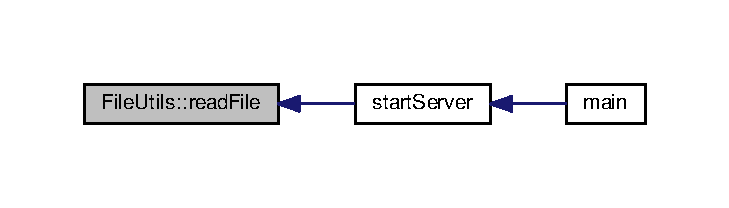
\includegraphics[width=350pt]{namespace_file_utils_ac71822c5146913486f67a3a1e7646155_icgraph}
\end{center}
\end{figure}



\hypertarget{namespace_generatable_chunked_temperature_world_typedefs}{\section{Generatable\-Chunked\-Temperature\-World\-Typedefs Namespace Reference}
\label{namespace_generatable_chunked_temperature_world_typedefs}\index{Generatable\-Chunked\-Temperature\-World\-Typedefs@{Generatable\-Chunked\-Temperature\-World\-Typedefs}}
}
\subsection*{Typedefs}
\begin{DoxyCompactItemize}
\item 
using \hyperlink{namespace_generatable_chunked_temperature_world_typedefs_a07d38658571f8f09839bc1bc8b105107}{Need\-Chunk\-Fn} = std\-::function$<$ bool(\hyperlink{struct_coord}{Coord}, \hyperlink{struct_coord}{Coord}, \hyperlink{struct_coord}{Coord})$>$
\item 
using \hyperlink{namespace_generatable_chunked_temperature_world_typedefs_a719e4469a105a21a76ed22274639c03a}{Make\-Chunk\-Fn} = std\-::function$<$ std\-::shared\-\_\-ptr$<$ \hyperlink{class_i_temperature_world_boundable}{I\-Temperature\-World\-Boundable}$<$ \hyperlink{class_i_temperature_world}{I\-Temperature\-World} $>$$>$(\hyperlink{struct_coord}{Coord}, \hyperlink{struct_coord}{Coord}, \hyperlink{struct_coord}{Coord})$>$
\end{DoxyCompactItemize}


\subsection{Typedef Documentation}
\hypertarget{namespace_generatable_chunked_temperature_world_typedefs_a719e4469a105a21a76ed22274639c03a}{\index{Generatable\-Chunked\-Temperature\-World\-Typedefs@{Generatable\-Chunked\-Temperature\-World\-Typedefs}!Make\-Chunk\-Fn@{Make\-Chunk\-Fn}}
\index{Make\-Chunk\-Fn@{Make\-Chunk\-Fn}!GeneratableChunkedTemperatureWorldTypedefs@{Generatable\-Chunked\-Temperature\-World\-Typedefs}}
\subsubsection[{Make\-Chunk\-Fn}]{\setlength{\rightskip}{0pt plus 5cm}using {\bf Generatable\-Chunked\-Temperature\-World\-Typedefs\-::\-Make\-Chunk\-Fn} = typedef std\-::function$<$std\-::shared\-\_\-ptr$<${\bf I\-Temperature\-World\-Boundable}$<${\bf I\-Temperature\-World}$>$$>$({\bf Coord}, {\bf Coord}, {\bf Coord})$>$}}\label{namespace_generatable_chunked_temperature_world_typedefs_a719e4469a105a21a76ed22274639c03a}
\hypertarget{namespace_generatable_chunked_temperature_world_typedefs_a07d38658571f8f09839bc1bc8b105107}{\index{Generatable\-Chunked\-Temperature\-World\-Typedefs@{Generatable\-Chunked\-Temperature\-World\-Typedefs}!Need\-Chunk\-Fn@{Need\-Chunk\-Fn}}
\index{Need\-Chunk\-Fn@{Need\-Chunk\-Fn}!GeneratableChunkedTemperatureWorldTypedefs@{Generatable\-Chunked\-Temperature\-World\-Typedefs}}
\subsubsection[{Need\-Chunk\-Fn}]{\setlength{\rightskip}{0pt plus 5cm}using {\bf Generatable\-Chunked\-Temperature\-World\-Typedefs\-::\-Need\-Chunk\-Fn} = typedef std\-::function$<$bool({\bf Coord}, {\bf Coord}, {\bf Coord})$>$}}\label{namespace_generatable_chunked_temperature_world_typedefs_a07d38658571f8f09839bc1bc8b105107}

\hypertarget{namespace_math_utils}{\section{Math\-Utils Namespace Reference}
\label{namespace_math_utils}\index{Math\-Utils@{Math\-Utils}}
}
\subsection*{Functions}
\begin{DoxyCompactItemize}
\item 
{\footnotesize template$<$typename T $>$ }\\T \hyperlink{namespace_math_utils_a32614fb8a04c557b66019693617ac7d5}{lerp} (T a, T b, double t)
\item 
double \hyperlink{namespace_math_utils_ad3b1d371a12fa3df8240630445c2eaf9}{random\-Float} ()
\end{DoxyCompactItemize}


\subsection{Detailed Description}
Collection of functions which work with numbers. 

\subsection{Function Documentation}
\hypertarget{namespace_math_utils_a32614fb8a04c557b66019693617ac7d5}{\index{Math\-Utils@{Math\-Utils}!lerp@{lerp}}
\index{lerp@{lerp}!MathUtils@{Math\-Utils}}
\subsubsection[{lerp}]{\setlength{\rightskip}{0pt plus 5cm}template$<$typename T $>$ T Math\-Utils\-::lerp (
\begin{DoxyParamCaption}
\item[{T}]{a, }
\item[{T}]{b, }
\item[{double}]{t}
\end{DoxyParamCaption}
)\hspace{0.3cm}{\ttfamily [inline]}}}\label{namespace_math_utils_a32614fb8a04c557b66019693617ac7d5}
Makes value {\ttfamily a} to be more \char`\"{}similar\char`\"{} to value {\ttfamily b} by factor {\ttfamily t}.


\begin{DoxyTemplParams}{Template Parameters}
{\em T} & Any number, e.\-g. {\ttfamily double}. \\
\hline
\end{DoxyTemplParams}

\begin{DoxyParams}{Parameters}
{\em a} & First value. \\
\hline
{\em b} & Second Value. \\
\hline
{\em t} & Factor. \\
\hline
\end{DoxyParams}
\begin{DoxyReturn}{Returns}
Linear interpolated value. 
\end{DoxyReturn}


Here is the caller graph for this function\-:
\nopagebreak
\begin{figure}[H]
\begin{center}
\leavevmode
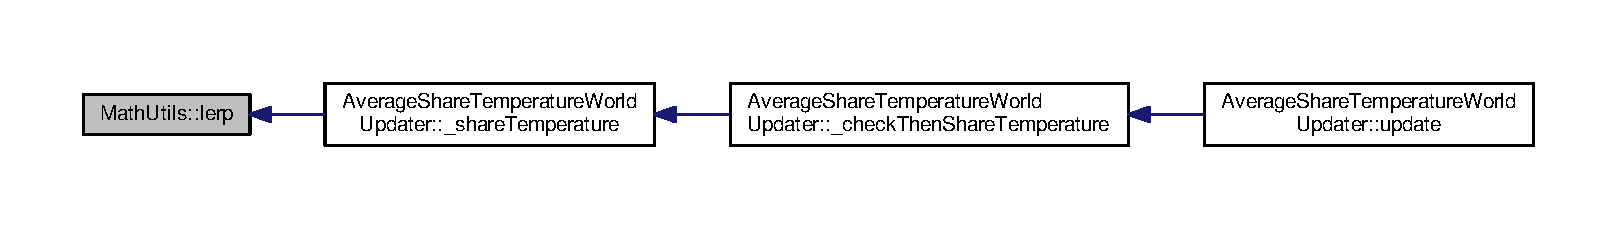
\includegraphics[width=350pt]{namespace_math_utils_a32614fb8a04c557b66019693617ac7d5_icgraph}
\end{center}
\end{figure}


\hypertarget{namespace_math_utils_ad3b1d371a12fa3df8240630445c2eaf9}{\index{Math\-Utils@{Math\-Utils}!random\-Float@{random\-Float}}
\index{random\-Float@{random\-Float}!MathUtils@{Math\-Utils}}
\subsubsection[{random\-Float}]{\setlength{\rightskip}{0pt plus 5cm}double Math\-Utils\-::random\-Float (
\begin{DoxyParamCaption}
{}
\end{DoxyParamCaption}
)\hspace{0.3cm}{\ttfamily [inline]}}}\label{namespace_math_utils_ad3b1d371a12fa3df8240630445c2eaf9}
Generates random value between 0.\-0 and 1.\-0.

\begin{DoxyReturn}{Returns}
Random value between 0.\-0 and 1.\-0. 
\end{DoxyReturn}


Here is the caller graph for this function\-:
\nopagebreak
\begin{figure}[H]
\begin{center}
\leavevmode
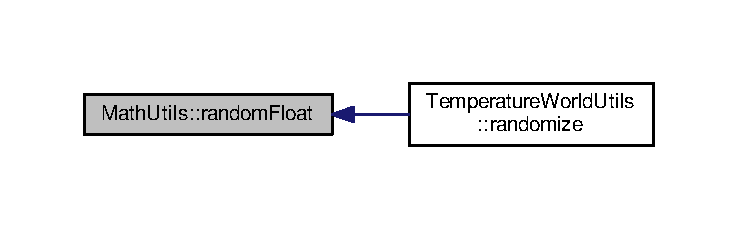
\includegraphics[width=350pt]{namespace_math_utils_ad3b1d371a12fa3df8240630445c2eaf9_icgraph}
\end{center}
\end{figure}



\hypertarget{namespace_temperature_world_utils}{\section{Temperature\-World\-Utils Namespace Reference}
\label{namespace_temperature_world_utils}\index{Temperature\-World\-Utils@{Temperature\-World\-Utils}}
}
\subsection*{Functions}
\begin{DoxyCompactItemize}
\item 
void \hyperlink{namespace_temperature_world_utils_ab11dd6f554d7b9ce4b7142bbb5dd7c2d}{randomize} (\hyperlink{class_i_temperature_world_boundable}{I\-Temperature\-World\-Boundable} \&world, \hyperlink{struct_temperature}{Temperature} min\-Temperature, \hyperlink{struct_temperature}{Temperature} max\-Temperature)
\end{DoxyCompactItemize}


\subsection{Detailed Description}
Collection of functions which work with temperature world. 

\subsection{Function Documentation}
\hypertarget{namespace_temperature_world_utils_ab11dd6f554d7b9ce4b7142bbb5dd7c2d}{\index{Temperature\-World\-Utils@{Temperature\-World\-Utils}!randomize@{randomize}}
\index{randomize@{randomize}!TemperatureWorldUtils@{Temperature\-World\-Utils}}
\subsubsection[{randomize}]{\setlength{\rightskip}{0pt plus 5cm}void Temperature\-World\-Utils\-::randomize (
\begin{DoxyParamCaption}
\item[{{\bf I\-Temperature\-World\-Boundable} \&}]{world, }
\item[{{\bf Temperature}}]{min\-Temperature, }
\item[{{\bf Temperature}}]{max\-Temperature}
\end{DoxyParamCaption}
)\hspace{0.3cm}{\ttfamily [inline]}}}\label{namespace_temperature_world_utils_ab11dd6f554d7b9ce4b7142bbb5dd7c2d}
Initializes temperature world with random temperatures. Random temperatures are generated within the range.


\begin{DoxyParams}{Parameters}
{\em world} & World to initialize. \\
\hline
{\em min\-Temperature} & Minimum possible temperature in the world. \\
\hline
{\em max\-Temperature} & Maximum possible temperature in the world. \\
\hline
\end{DoxyParams}


Here is the call graph for this function\-:
\nopagebreak
\begin{figure}[H]
\begin{center}
\leavevmode
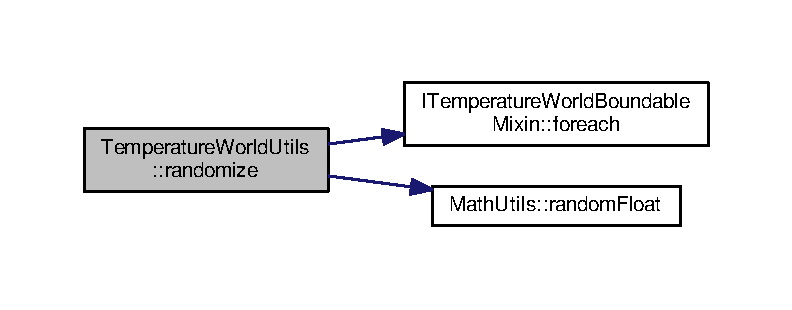
\includegraphics[width=350pt]{namespace_temperature_world_utils_ab11dd6f554d7b9ce4b7142bbb5dd7c2d_cgraph}
\end{center}
\end{figure}



\hypertarget{namespace_time_utils}{\section{Time\-Utils Namespace Reference}
\label{namespace_time_utils}\index{Time\-Utils@{Time\-Utils}}
}
\subsection*{Functions}
\begin{DoxyCompactItemize}
\item 
long long int \hyperlink{namespace_time_utils_abbc5c960cc2615a98fee89b6855b2460}{current\-Time\-Millis} ()
\item 
double \hyperlink{namespace_time_utils_a687d4373b853931d7206dfbd9fde704f}{current\-Time\-Seconds} ()
\end{DoxyCompactItemize}


\subsection{Detailed Description}
Collection of functions which work with time. 

\subsection{Function Documentation}
\hypertarget{namespace_time_utils_abbc5c960cc2615a98fee89b6855b2460}{\index{Time\-Utils@{Time\-Utils}!current\-Time\-Millis@{current\-Time\-Millis}}
\index{current\-Time\-Millis@{current\-Time\-Millis}!TimeUtils@{Time\-Utils}}
\subsubsection[{current\-Time\-Millis}]{\setlength{\rightskip}{0pt plus 5cm}long long int Time\-Utils\-::current\-Time\-Millis (
\begin{DoxyParamCaption}
{}
\end{DoxyParamCaption}
)\hspace{0.3cm}{\ttfamily [inline]}}}\label{namespace_time_utils_abbc5c960cc2615a98fee89b6855b2460}
Gets current time since Epoch in milliseconds.

\begin{DoxyReturn}{Returns}
Milliseconds since Epoch. 
\end{DoxyReturn}


Here is the caller graph for this function\-:
\nopagebreak
\begin{figure}[H]
\begin{center}
\leavevmode
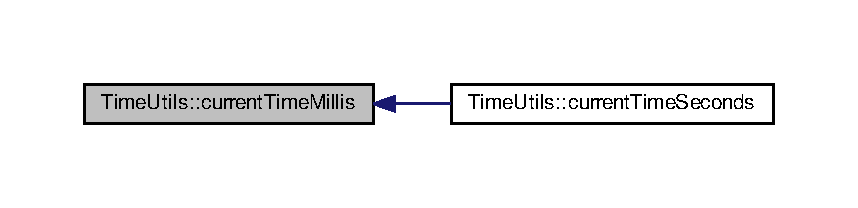
\includegraphics[width=350pt]{namespace_time_utils_abbc5c960cc2615a98fee89b6855b2460_icgraph}
\end{center}
\end{figure}


\hypertarget{namespace_time_utils_a687d4373b853931d7206dfbd9fde704f}{\index{Time\-Utils@{Time\-Utils}!current\-Time\-Seconds@{current\-Time\-Seconds}}
\index{current\-Time\-Seconds@{current\-Time\-Seconds}!TimeUtils@{Time\-Utils}}
\subsubsection[{current\-Time\-Seconds}]{\setlength{\rightskip}{0pt plus 5cm}double Time\-Utils\-::current\-Time\-Seconds (
\begin{DoxyParamCaption}
{}
\end{DoxyParamCaption}
)\hspace{0.3cm}{\ttfamily [inline]}}}\label{namespace_time_utils_a687d4373b853931d7206dfbd9fde704f}
Gets current time since Epoch in seconds.

\begin{DoxyReturn}{Returns}
Seconds since Epoch. 
\end{DoxyReturn}


Here is the call graph for this function\-:
\nopagebreak
\begin{figure}[H]
\begin{center}
\leavevmode
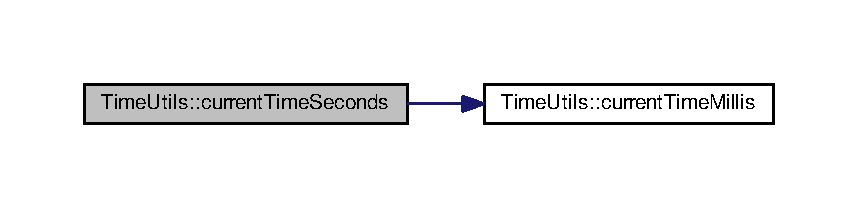
\includegraphics[width=350pt]{namespace_time_utils_a687d4373b853931d7206dfbd9fde704f_cgraph}
\end{center}
\end{figure}



\chapter{Class Documentation}
\hypertarget{class_average_share_temperature_world_updater}{\section{Average\-Share\-Temperature\-World\-Updater Class Reference}
\label{class_average_share_temperature_world_updater}\index{Average\-Share\-Temperature\-World\-Updater@{Average\-Share\-Temperature\-World\-Updater}}
}


{\ttfamily \#include $<$Average\-Share\-Temperature\-World\-Updater.\-hpp$>$}



Inheritance diagram for Average\-Share\-Temperature\-World\-Updater\-:
\nopagebreak
\begin{figure}[H]
\begin{center}
\leavevmode
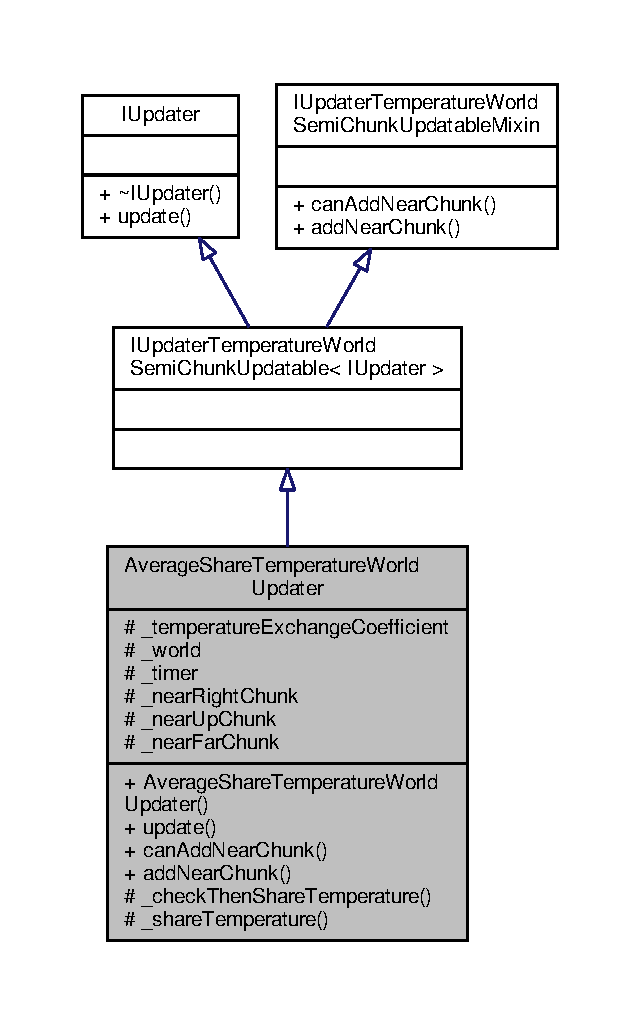
\includegraphics[width=307pt]{class_average_share_temperature_world_updater__inherit__graph}
\end{center}
\end{figure}


Collaboration diagram for Average\-Share\-Temperature\-World\-Updater\-:
\nopagebreak
\begin{figure}[H]
\begin{center}
\leavevmode
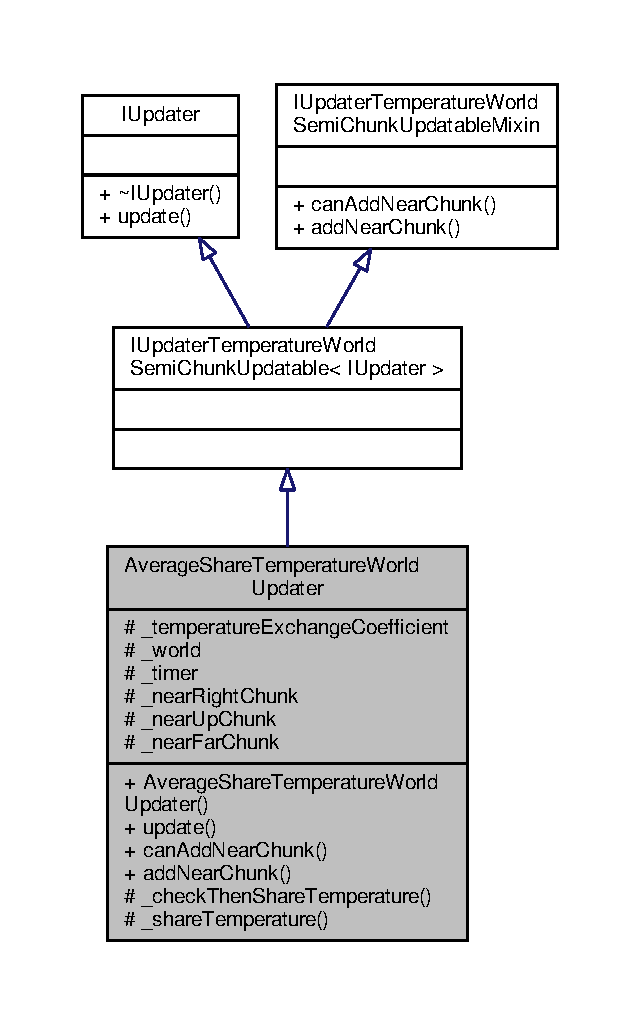
\includegraphics[width=307pt]{class_average_share_temperature_world_updater__coll__graph}
\end{center}
\end{figure}
\subsection*{Public Member Functions}
\begin{DoxyCompactItemize}
\item 
\hyperlink{class_average_share_temperature_world_updater_a0031a5c20f9b717f0eb099f1d69e5ced}{Average\-Share\-Temperature\-World\-Updater} (double temperature\-Exchange\-Coefficient, std\-::shared\-\_\-ptr$<$ \hyperlink{class_i_temperature_world_boundable}{I\-Temperature\-World\-Boundable}$<$ \hyperlink{class_i_temperature_world}{I\-Temperature\-World} $>$$>$ world, std\-::shared\-\_\-ptr$<$ \hyperlink{class_i_timer_blockable}{I\-Timer\-Blockable}$<$ \hyperlink{class_i_timer}{I\-Timer} $>$$>$ timer)
\item 
void \hyperlink{class_average_share_temperature_world_updater_a29be9be2073572f3ef2dc5315c506245}{update} () override
\item 
bool \hyperlink{class_average_share_temperature_world_updater_a2b3403ad5d9c7ef2f39b359fc87f44b8}{can\-Add\-Near\-Chunk} (\hyperlink{_edge_8hpp_a5be7c8fa582f7b873d1c6caacb633073}{Edge} edge, const std\-::shared\-\_\-ptr$<$ \hyperlink{class_i_temperature_world_boundable}{I\-Temperature\-World\-Boundable}$<$ \hyperlink{class_i_temperature_world}{I\-Temperature\-World} $>$$>$ \&chunk) const noexceptoverride
\item 
void \hyperlink{class_average_share_temperature_world_updater_ab48c277317950d9b9e571d13f3461307}{add\-Near\-Chunk} (\hyperlink{_edge_8hpp_a5be7c8fa582f7b873d1c6caacb633073}{Edge} edge, std\-::shared\-\_\-ptr$<$ \hyperlink{class_i_temperature_world_boundable}{I\-Temperature\-World\-Boundable}$<$ \hyperlink{class_i_temperature_world}{I\-Temperature\-World} $>$$>$ chunk) override
\end{DoxyCompactItemize}
\subsection*{Protected Member Functions}
\begin{DoxyCompactItemize}
\item 
void \hyperlink{class_average_share_temperature_world_updater_ad117315f70e5a2e214547dbf789715f8}{\-\_\-check\-Then\-Share\-Temperature} (double dt, const std\-::shared\-\_\-ptr$<$ \hyperlink{class_i_temperature_world_boundable}{I\-Temperature\-World\-Boundable}$<$ \hyperlink{class_i_temperature_world}{I\-Temperature\-World} $>$$>$ \&first\-World, \hyperlink{struct_coord}{Coord} x, \hyperlink{struct_coord}{Coord} y, \hyperlink{struct_coord}{Coord} z, const std\-::shared\-\_\-ptr$<$ \hyperlink{class_i_temperature_world_boundable}{I\-Temperature\-World\-Boundable}$<$ \hyperlink{class_i_temperature_world}{I\-Temperature\-World} $>$$>$ \&second\-World, \hyperlink{struct_coord}{Coord} next\-X, \hyperlink{struct_coord}{Coord} next\-Y, \hyperlink{struct_coord}{Coord} next\-Z)
\item 
void \hyperlink{class_average_share_temperature_world_updater_ab5fe8bcd2311e4af0b4a09d5f3d7b8d9}{\-\_\-share\-Temperature} (double dt, const std\-::shared\-\_\-ptr$<$ \hyperlink{class_i_temperature_world_boundable}{I\-Temperature\-World\-Boundable}$<$ \hyperlink{class_i_temperature_world}{I\-Temperature\-World} $>$$>$ \&first\-World, \hyperlink{struct_coord}{Coord} x, \hyperlink{struct_coord}{Coord} y, \hyperlink{struct_coord}{Coord} z, const std\-::shared\-\_\-ptr$<$ \hyperlink{class_i_temperature_world_boundable}{I\-Temperature\-World\-Boundable}$<$ \hyperlink{class_i_temperature_world}{I\-Temperature\-World} $>$$>$ \&second\-World, \hyperlink{struct_coord}{Coord} next\-X, \hyperlink{struct_coord}{Coord} next\-Y, \hyperlink{struct_coord}{Coord} next\-Z)
\end{DoxyCompactItemize}
\subsection*{Protected Attributes}
\begin{DoxyCompactItemize}
\item 
double \hyperlink{class_average_share_temperature_world_updater_a37ebe90d538e148a8da4efa0845d334c}{\-\_\-temperature\-Exchange\-Coefficient}
\item 
std\-::shared\-\_\-ptr\\*
$<$ \hyperlink{class_i_temperature_world_boundable}{I\-Temperature\-World\-Boundable}\\*
$<$ \hyperlink{class_i_temperature_world}{I\-Temperature\-World} $>$ $>$ \hyperlink{class_average_share_temperature_world_updater_a7327a9c0043f7fd278edcc1e7b7ecf78}{\-\_\-world}
\item 
std\-::shared\-\_\-ptr\\*
$<$ \hyperlink{class_i_timer_blockable}{I\-Timer\-Blockable}$<$ \hyperlink{class_i_timer}{I\-Timer} $>$ $>$ \hyperlink{class_average_share_temperature_world_updater_acc17234a8b1f33e1be9c7806e4973be3}{\-\_\-timer}
\item 
std\-::shared\-\_\-ptr\\*
$<$ \hyperlink{class_i_temperature_world_boundable}{I\-Temperature\-World\-Boundable}\\*
$<$ \hyperlink{class_i_temperature_world}{I\-Temperature\-World} $>$ $>$ \hyperlink{class_average_share_temperature_world_updater_a1e5e2936bb7b6613a27129a2a199247d}{\-\_\-near\-Right\-Chunk}
\item 
std\-::shared\-\_\-ptr\\*
$<$ \hyperlink{class_i_temperature_world_boundable}{I\-Temperature\-World\-Boundable}\\*
$<$ \hyperlink{class_i_temperature_world}{I\-Temperature\-World} $>$ $>$ \hyperlink{class_average_share_temperature_world_updater_a33ced05d90444ec05a0fc531d9c1fa7f}{\-\_\-near\-Up\-Chunk}
\item 
std\-::shared\-\_\-ptr\\*
$<$ \hyperlink{class_i_temperature_world_boundable}{I\-Temperature\-World\-Boundable}\\*
$<$ \hyperlink{class_i_temperature_world}{I\-Temperature\-World} $>$ $>$ \hyperlink{class_average_share_temperature_world_updater_a0164e9a5b9b614a3fb6fc360d4c0864a}{\-\_\-near\-Far\-Chunk}
\end{DoxyCompactItemize}


\subsection{Detailed Description}
Implementation of temperature world updater.

How it works for every two cells\-:
\begin{DoxyEnumerate}
\item Computes average of temperatures of two cells.
\item Brings temperature of each cell to this average world. Speed is determined by temperature exchange coefficient. 
\end{DoxyEnumerate}

\subsection{Constructor \& Destructor Documentation}
\hypertarget{class_average_share_temperature_world_updater_a0031a5c20f9b717f0eb099f1d69e5ced}{\index{Average\-Share\-Temperature\-World\-Updater@{Average\-Share\-Temperature\-World\-Updater}!Average\-Share\-Temperature\-World\-Updater@{Average\-Share\-Temperature\-World\-Updater}}
\index{Average\-Share\-Temperature\-World\-Updater@{Average\-Share\-Temperature\-World\-Updater}!AverageShareTemperatureWorldUpdater@{Average\-Share\-Temperature\-World\-Updater}}
\subsubsection[{Average\-Share\-Temperature\-World\-Updater}]{\setlength{\rightskip}{0pt plus 5cm}Average\-Share\-Temperature\-World\-Updater\-::\-Average\-Share\-Temperature\-World\-Updater (
\begin{DoxyParamCaption}
\item[{double}]{temperature\-Exchange\-Coefficient, }
\item[{std\-::shared\-\_\-ptr$<$ {\bf I\-Temperature\-World\-Boundable}$<$ {\bf I\-Temperature\-World} $>$$>$}]{world, }
\item[{std\-::shared\-\_\-ptr$<$ {\bf I\-Timer\-Blockable}$<$ {\bf I\-Timer} $>$$>$}]{timer}
\end{DoxyParamCaption}
)}}\label{class_average_share_temperature_world_updater_a0031a5c20f9b717f0eb099f1d69e5ced}


\subsection{Member Function Documentation}
\hypertarget{class_average_share_temperature_world_updater_ad117315f70e5a2e214547dbf789715f8}{\index{Average\-Share\-Temperature\-World\-Updater@{Average\-Share\-Temperature\-World\-Updater}!\-\_\-check\-Then\-Share\-Temperature@{\-\_\-check\-Then\-Share\-Temperature}}
\index{\-\_\-check\-Then\-Share\-Temperature@{\-\_\-check\-Then\-Share\-Temperature}!AverageShareTemperatureWorldUpdater@{Average\-Share\-Temperature\-World\-Updater}}
\subsubsection[{\-\_\-check\-Then\-Share\-Temperature}]{\setlength{\rightskip}{0pt plus 5cm}void Average\-Share\-Temperature\-World\-Updater\-::\-\_\-check\-Then\-Share\-Temperature (
\begin{DoxyParamCaption}
\item[{double}]{dt, }
\item[{const std\-::shared\-\_\-ptr$<$ {\bf I\-Temperature\-World\-Boundable}$<$ {\bf I\-Temperature\-World} $>$$>$ \&}]{first\-World, }
\item[{{\bf Coord}}]{x, }
\item[{{\bf Coord}}]{y, }
\item[{{\bf Coord}}]{z, }
\item[{const std\-::shared\-\_\-ptr$<$ {\bf I\-Temperature\-World\-Boundable}$<$ {\bf I\-Temperature\-World} $>$$>$ \&}]{second\-World, }
\item[{{\bf Coord}}]{next\-X, }
\item[{{\bf Coord}}]{next\-Y, }
\item[{{\bf Coord}}]{next\-Z}
\end{DoxyParamCaption}
)\hspace{0.3cm}{\ttfamily [protected]}}}\label{class_average_share_temperature_world_updater_ad117315f70e5a2e214547dbf789715f8}


Here is the call graph for this function\-:
\nopagebreak
\begin{figure}[H]
\begin{center}
\leavevmode
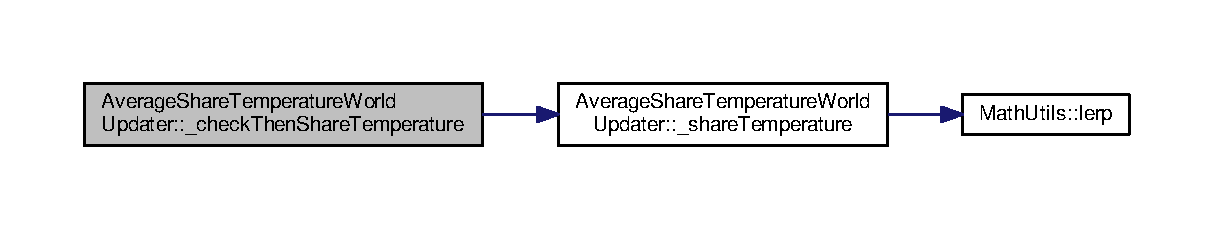
\includegraphics[width=350pt]{class_average_share_temperature_world_updater_ad117315f70e5a2e214547dbf789715f8_cgraph}
\end{center}
\end{figure}




Here is the caller graph for this function\-:
\nopagebreak
\begin{figure}[H]
\begin{center}
\leavevmode
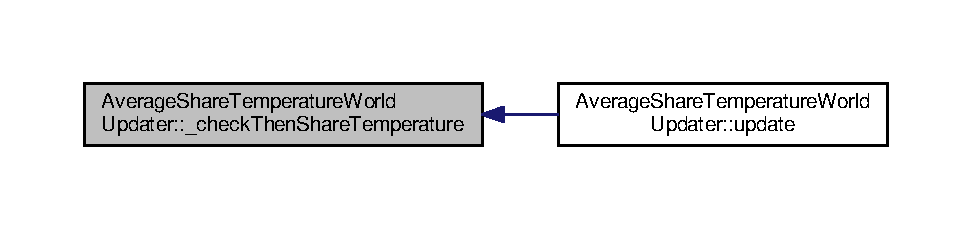
\includegraphics[width=350pt]{class_average_share_temperature_world_updater_ad117315f70e5a2e214547dbf789715f8_icgraph}
\end{center}
\end{figure}


\hypertarget{class_average_share_temperature_world_updater_ab5fe8bcd2311e4af0b4a09d5f3d7b8d9}{\index{Average\-Share\-Temperature\-World\-Updater@{Average\-Share\-Temperature\-World\-Updater}!\-\_\-share\-Temperature@{\-\_\-share\-Temperature}}
\index{\-\_\-share\-Temperature@{\-\_\-share\-Temperature}!AverageShareTemperatureWorldUpdater@{Average\-Share\-Temperature\-World\-Updater}}
\subsubsection[{\-\_\-share\-Temperature}]{\setlength{\rightskip}{0pt plus 5cm}void Average\-Share\-Temperature\-World\-Updater\-::\-\_\-share\-Temperature (
\begin{DoxyParamCaption}
\item[{double}]{dt, }
\item[{const std\-::shared\-\_\-ptr$<$ {\bf I\-Temperature\-World\-Boundable}$<$ {\bf I\-Temperature\-World} $>$$>$ \&}]{first\-World, }
\item[{{\bf Coord}}]{x, }
\item[{{\bf Coord}}]{y, }
\item[{{\bf Coord}}]{z, }
\item[{const std\-::shared\-\_\-ptr$<$ {\bf I\-Temperature\-World\-Boundable}$<$ {\bf I\-Temperature\-World} $>$$>$ \&}]{second\-World, }
\item[{{\bf Coord}}]{next\-X, }
\item[{{\bf Coord}}]{next\-Y, }
\item[{{\bf Coord}}]{next\-Z}
\end{DoxyParamCaption}
)\hspace{0.3cm}{\ttfamily [protected]}}}\label{class_average_share_temperature_world_updater_ab5fe8bcd2311e4af0b4a09d5f3d7b8d9}


Here is the call graph for this function\-:
\nopagebreak
\begin{figure}[H]
\begin{center}
\leavevmode
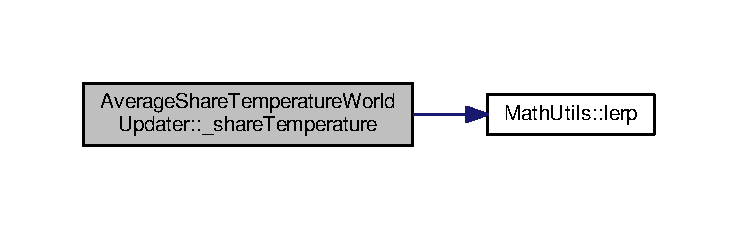
\includegraphics[width=350pt]{class_average_share_temperature_world_updater_ab5fe8bcd2311e4af0b4a09d5f3d7b8d9_cgraph}
\end{center}
\end{figure}




Here is the caller graph for this function\-:
\nopagebreak
\begin{figure}[H]
\begin{center}
\leavevmode
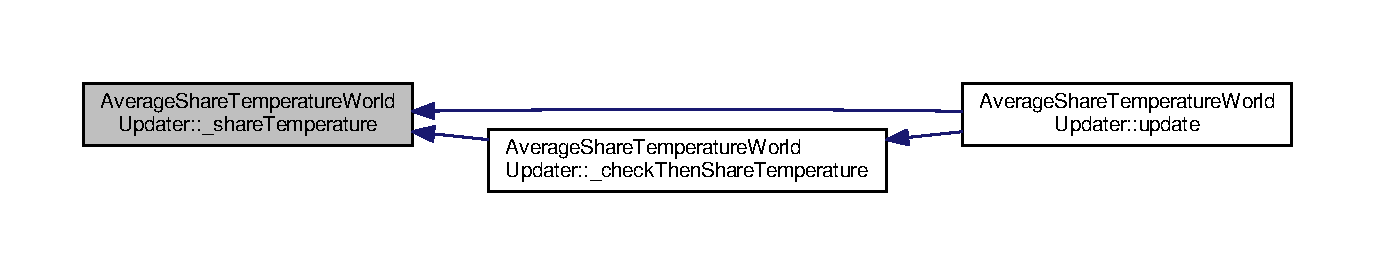
\includegraphics[width=350pt]{class_average_share_temperature_world_updater_ab5fe8bcd2311e4af0b4a09d5f3d7b8d9_icgraph}
\end{center}
\end{figure}


\hypertarget{class_average_share_temperature_world_updater_ab48c277317950d9b9e571d13f3461307}{\index{Average\-Share\-Temperature\-World\-Updater@{Average\-Share\-Temperature\-World\-Updater}!add\-Near\-Chunk@{add\-Near\-Chunk}}
\index{add\-Near\-Chunk@{add\-Near\-Chunk}!AverageShareTemperatureWorldUpdater@{Average\-Share\-Temperature\-World\-Updater}}
\subsubsection[{add\-Near\-Chunk}]{\setlength{\rightskip}{0pt plus 5cm}void Average\-Share\-Temperature\-World\-Updater\-::add\-Near\-Chunk (
\begin{DoxyParamCaption}
\item[{{\bf Edge}}]{edge, }
\item[{std\-::shared\-\_\-ptr$<$ {\bf I\-Temperature\-World\-Boundable}$<$ {\bf I\-Temperature\-World} $>$$>$}]{other\-Chunk}
\end{DoxyParamCaption}
)\hspace{0.3cm}{\ttfamily [override]}, {\ttfamily [virtual]}}}\label{class_average_share_temperature_world_updater_ab48c277317950d9b9e571d13f3461307}
Adds chunk to near chunks collection on specified edge.


\begin{DoxyParams}{Parameters}
{\em other\-Chunk} & Near chunk. \\
\hline
\end{DoxyParams}


Implements \hyperlink{class_i_updater_temperature_world_semi_chunk_updatable_mixin_aa3139125095140f797df3cebb466c48a}{I\-Updater\-Temperature\-World\-Semi\-Chunk\-Updatable\-Mixin}.



Here is the call graph for this function\-:
\nopagebreak
\begin{figure}[H]
\begin{center}
\leavevmode
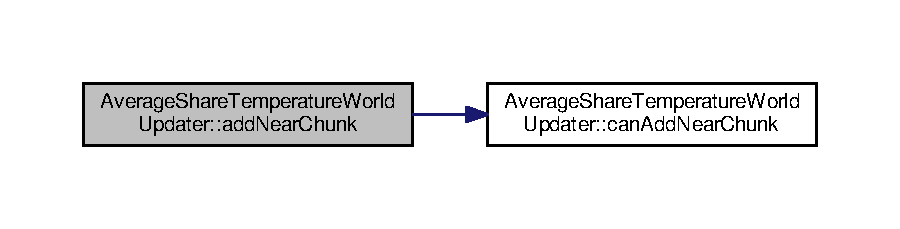
\includegraphics[width=350pt]{class_average_share_temperature_world_updater_ab48c277317950d9b9e571d13f3461307_cgraph}
\end{center}
\end{figure}


\hypertarget{class_average_share_temperature_world_updater_a2b3403ad5d9c7ef2f39b359fc87f44b8}{\index{Average\-Share\-Temperature\-World\-Updater@{Average\-Share\-Temperature\-World\-Updater}!can\-Add\-Near\-Chunk@{can\-Add\-Near\-Chunk}}
\index{can\-Add\-Near\-Chunk@{can\-Add\-Near\-Chunk}!AverageShareTemperatureWorldUpdater@{Average\-Share\-Temperature\-World\-Updater}}
\subsubsection[{can\-Add\-Near\-Chunk}]{\setlength{\rightskip}{0pt plus 5cm}bool Average\-Share\-Temperature\-World\-Updater\-::can\-Add\-Near\-Chunk (
\begin{DoxyParamCaption}
\item[{{\bf Edge}}]{edge, }
\item[{const std\-::shared\-\_\-ptr$<$ {\bf I\-Temperature\-World\-Boundable}$<$ {\bf I\-Temperature\-World} $>$$>$ \&}]{other\-Chunk}
\end{DoxyParamCaption}
) const\hspace{0.3cm}{\ttfamily [override]}, {\ttfamily [virtual]}, {\ttfamily [noexcept]}}}\label{class_average_share_temperature_world_updater_a2b3403ad5d9c7ef2f39b359fc87f44b8}
Tells whether it's possible to add this chunk to near chunks collection on specified edge. This method is thread-\/safe.


\begin{DoxyParams}{Parameters}
{\em other\-Chunk} & Near chunk. \\
\hline
\end{DoxyParams}
\begin{DoxyReturn}{Returns}
True if this chunk can be added to near chunks collection. 
\end{DoxyReturn}


Implements \hyperlink{class_i_updater_temperature_world_semi_chunk_updatable_mixin_a35d2d34bcf2f9e857246bd8d92aec74f}{I\-Updater\-Temperature\-World\-Semi\-Chunk\-Updatable\-Mixin}.



Here is the caller graph for this function\-:
\nopagebreak
\begin{figure}[H]
\begin{center}
\leavevmode
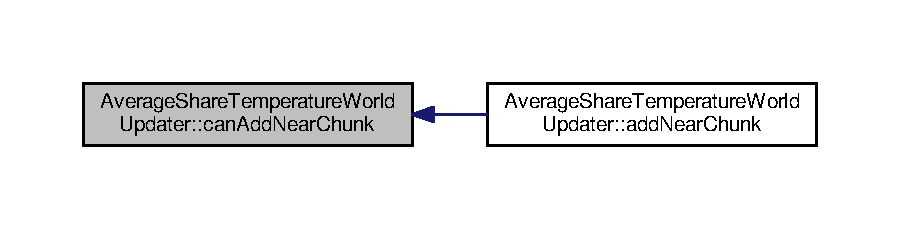
\includegraphics[width=350pt]{class_average_share_temperature_world_updater_a2b3403ad5d9c7ef2f39b359fc87f44b8_icgraph}
\end{center}
\end{figure}


\hypertarget{class_average_share_temperature_world_updater_a29be9be2073572f3ef2dc5315c506245}{\index{Average\-Share\-Temperature\-World\-Updater@{Average\-Share\-Temperature\-World\-Updater}!update@{update}}
\index{update@{update}!AverageShareTemperatureWorldUpdater@{Average\-Share\-Temperature\-World\-Updater}}
\subsubsection[{update}]{\setlength{\rightskip}{0pt plus 5cm}void Average\-Share\-Temperature\-World\-Updater\-::update (
\begin{DoxyParamCaption}
{}
\end{DoxyParamCaption}
)\hspace{0.3cm}{\ttfamily [override]}, {\ttfamily [virtual]}}}\label{class_average_share_temperature_world_updater_a29be9be2073572f3ef2dc5315c506245}
Updates. 

Implements \hyperlink{class_i_updater_a08a8af34922a2320f5ab5617e6e31276}{I\-Updater}.



Here is the call graph for this function\-:
\nopagebreak
\begin{figure}[H]
\begin{center}
\leavevmode
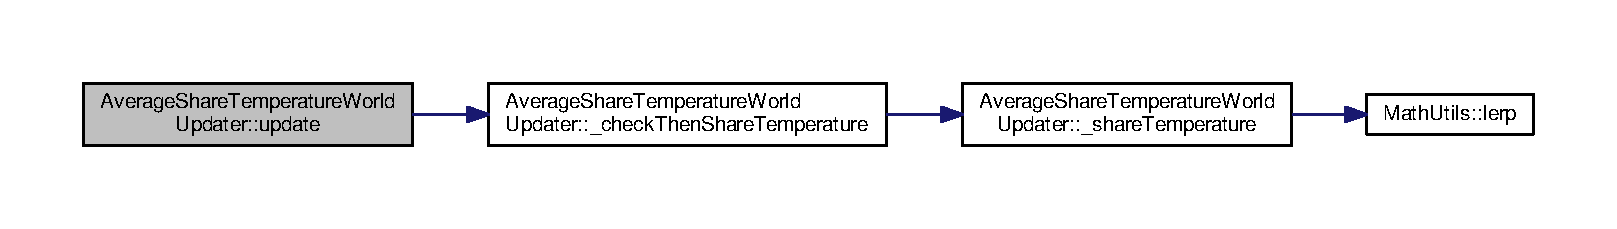
\includegraphics[width=350pt]{class_average_share_temperature_world_updater_a29be9be2073572f3ef2dc5315c506245_cgraph}
\end{center}
\end{figure}




\subsection{Member Data Documentation}
\hypertarget{class_average_share_temperature_world_updater_a0164e9a5b9b614a3fb6fc360d4c0864a}{\index{Average\-Share\-Temperature\-World\-Updater@{Average\-Share\-Temperature\-World\-Updater}!\-\_\-near\-Far\-Chunk@{\-\_\-near\-Far\-Chunk}}
\index{\-\_\-near\-Far\-Chunk@{\-\_\-near\-Far\-Chunk}!AverageShareTemperatureWorldUpdater@{Average\-Share\-Temperature\-World\-Updater}}
\subsubsection[{\-\_\-near\-Far\-Chunk}]{\setlength{\rightskip}{0pt plus 5cm}std\-::shared\-\_\-ptr$<${\bf I\-Temperature\-World\-Boundable}$<${\bf I\-Temperature\-World}$>$ $>$ Average\-Share\-Temperature\-World\-Updater\-::\-\_\-near\-Far\-Chunk\hspace{0.3cm}{\ttfamily [protected]}}}\label{class_average_share_temperature_world_updater_a0164e9a5b9b614a3fb6fc360d4c0864a}
\hypertarget{class_average_share_temperature_world_updater_a1e5e2936bb7b6613a27129a2a199247d}{\index{Average\-Share\-Temperature\-World\-Updater@{Average\-Share\-Temperature\-World\-Updater}!\-\_\-near\-Right\-Chunk@{\-\_\-near\-Right\-Chunk}}
\index{\-\_\-near\-Right\-Chunk@{\-\_\-near\-Right\-Chunk}!AverageShareTemperatureWorldUpdater@{Average\-Share\-Temperature\-World\-Updater}}
\subsubsection[{\-\_\-near\-Right\-Chunk}]{\setlength{\rightskip}{0pt plus 5cm}std\-::shared\-\_\-ptr$<${\bf I\-Temperature\-World\-Boundable}$<${\bf I\-Temperature\-World}$>$ $>$ Average\-Share\-Temperature\-World\-Updater\-::\-\_\-near\-Right\-Chunk\hspace{0.3cm}{\ttfamily [protected]}}}\label{class_average_share_temperature_world_updater_a1e5e2936bb7b6613a27129a2a199247d}
\hypertarget{class_average_share_temperature_world_updater_a33ced05d90444ec05a0fc531d9c1fa7f}{\index{Average\-Share\-Temperature\-World\-Updater@{Average\-Share\-Temperature\-World\-Updater}!\-\_\-near\-Up\-Chunk@{\-\_\-near\-Up\-Chunk}}
\index{\-\_\-near\-Up\-Chunk@{\-\_\-near\-Up\-Chunk}!AverageShareTemperatureWorldUpdater@{Average\-Share\-Temperature\-World\-Updater}}
\subsubsection[{\-\_\-near\-Up\-Chunk}]{\setlength{\rightskip}{0pt plus 5cm}std\-::shared\-\_\-ptr$<${\bf I\-Temperature\-World\-Boundable}$<${\bf I\-Temperature\-World}$>$ $>$ Average\-Share\-Temperature\-World\-Updater\-::\-\_\-near\-Up\-Chunk\hspace{0.3cm}{\ttfamily [protected]}}}\label{class_average_share_temperature_world_updater_a33ced05d90444ec05a0fc531d9c1fa7f}
\hypertarget{class_average_share_temperature_world_updater_a37ebe90d538e148a8da4efa0845d334c}{\index{Average\-Share\-Temperature\-World\-Updater@{Average\-Share\-Temperature\-World\-Updater}!\-\_\-temperature\-Exchange\-Coefficient@{\-\_\-temperature\-Exchange\-Coefficient}}
\index{\-\_\-temperature\-Exchange\-Coefficient@{\-\_\-temperature\-Exchange\-Coefficient}!AverageShareTemperatureWorldUpdater@{Average\-Share\-Temperature\-World\-Updater}}
\subsubsection[{\-\_\-temperature\-Exchange\-Coefficient}]{\setlength{\rightskip}{0pt plus 5cm}double Average\-Share\-Temperature\-World\-Updater\-::\-\_\-temperature\-Exchange\-Coefficient\hspace{0.3cm}{\ttfamily [protected]}}}\label{class_average_share_temperature_world_updater_a37ebe90d538e148a8da4efa0845d334c}
\hypertarget{class_average_share_temperature_world_updater_acc17234a8b1f33e1be9c7806e4973be3}{\index{Average\-Share\-Temperature\-World\-Updater@{Average\-Share\-Temperature\-World\-Updater}!\-\_\-timer@{\-\_\-timer}}
\index{\-\_\-timer@{\-\_\-timer}!AverageShareTemperatureWorldUpdater@{Average\-Share\-Temperature\-World\-Updater}}
\subsubsection[{\-\_\-timer}]{\setlength{\rightskip}{0pt plus 5cm}std\-::shared\-\_\-ptr$<${\bf I\-Timer\-Blockable}$<${\bf I\-Timer}$>$ $>$ Average\-Share\-Temperature\-World\-Updater\-::\-\_\-timer\hspace{0.3cm}{\ttfamily [protected]}}}\label{class_average_share_temperature_world_updater_acc17234a8b1f33e1be9c7806e4973be3}
\hypertarget{class_average_share_temperature_world_updater_a7327a9c0043f7fd278edcc1e7b7ecf78}{\index{Average\-Share\-Temperature\-World\-Updater@{Average\-Share\-Temperature\-World\-Updater}!\-\_\-world@{\-\_\-world}}
\index{\-\_\-world@{\-\_\-world}!AverageShareTemperatureWorldUpdater@{Average\-Share\-Temperature\-World\-Updater}}
\subsubsection[{\-\_\-world}]{\setlength{\rightskip}{0pt plus 5cm}std\-::shared\-\_\-ptr$<${\bf I\-Temperature\-World\-Boundable}$<${\bf I\-Temperature\-World}$>$ $>$ Average\-Share\-Temperature\-World\-Updater\-::\-\_\-world\hspace{0.3cm}{\ttfamily [protected]}}}\label{class_average_share_temperature_world_updater_a7327a9c0043f7fd278edcc1e7b7ecf78}


The documentation for this class was generated from the following files\-:\begin{DoxyCompactItemize}
\item 
/home/travis/build/glitchless/\-Recast/src/headers/temperature-\/world/implementation/\hyperlink{_average_share_temperature_world_updater_8hpp}{Average\-Share\-Temperature\-World\-Updater.\-hpp}\item 
/home/travis/build/glitchless/\-Recast/src/temperature-\/world/implementation/\hyperlink{_average_share_temperature_world_updater_8cpp}{Average\-Share\-Temperature\-World\-Updater.\-cpp}\end{DoxyCompactItemize}

\hypertarget{class_basic_timer}{\section{Basic\-Timer Class Reference}
\label{class_basic_timer}\index{Basic\-Timer@{Basic\-Timer}}
}


{\ttfamily \#include $<$Basic\-Timer.\-hpp$>$}



Inheritance diagram for Basic\-Timer\-:
\nopagebreak
\begin{figure}[H]
\begin{center}
\leavevmode
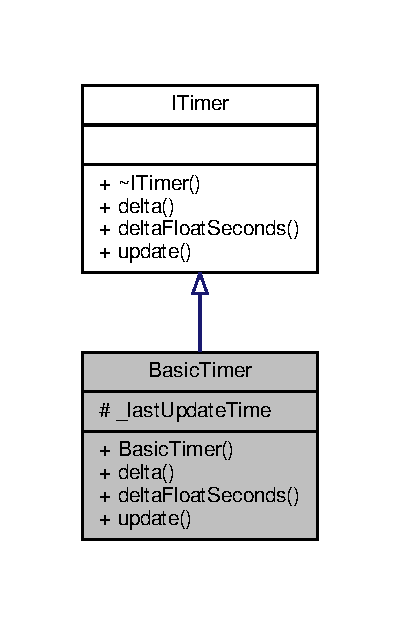
\includegraphics[width=192pt]{class_basic_timer__inherit__graph}
\end{center}
\end{figure}


Collaboration diagram for Basic\-Timer\-:
\nopagebreak
\begin{figure}[H]
\begin{center}
\leavevmode
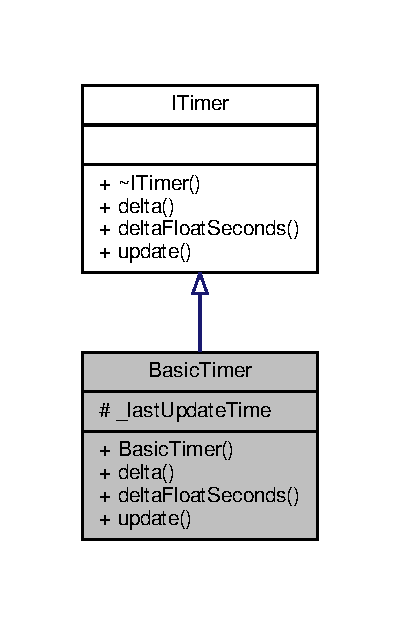
\includegraphics[width=192pt]{class_basic_timer__coll__graph}
\end{center}
\end{figure}
\subsection*{Public Member Functions}
\begin{DoxyCompactItemize}
\item 
\hyperlink{class_basic_timer_ab557401ac85db6cf5fc7ffcebc119811}{Basic\-Timer} ()
\item 
std\-::chrono\-::milliseconds \hyperlink{class_basic_timer_a49bc91a549323a1a7fc6b7d9ec727174}{delta} () const 
\item 
double \hyperlink{class_basic_timer_afbe3d01b15f26573eb12c04ae7c28684}{delta\-Float\-Seconds} () const 
\item 
void \hyperlink{class_basic_timer_abf76823ef1c782a0c6d49af2652b5271}{update} ()
\end{DoxyCompactItemize}
\subsection*{Protected Attributes}
\begin{DoxyCompactItemize}
\item 
std\-::chrono\-::system\-\_\-clock\-::time\-\_\-point \hyperlink{class_basic_timer_a1c5ab332f195b367d5fbf91183f4dc8a}{\-\_\-last\-Update\-Time}
\end{DoxyCompactItemize}


\subsection{Detailed Description}
Timer that measures time duration between two updates. 

\subsection{Constructor \& Destructor Documentation}
\hypertarget{class_basic_timer_ab557401ac85db6cf5fc7ffcebc119811}{\index{Basic\-Timer@{Basic\-Timer}!Basic\-Timer@{Basic\-Timer}}
\index{Basic\-Timer@{Basic\-Timer}!BasicTimer@{Basic\-Timer}}
\subsubsection[{Basic\-Timer}]{\setlength{\rightskip}{0pt plus 5cm}Basic\-Timer\-::\-Basic\-Timer (
\begin{DoxyParamCaption}
{}
\end{DoxyParamCaption}
)}}\label{class_basic_timer_ab557401ac85db6cf5fc7ffcebc119811}


\subsection{Member Function Documentation}
\hypertarget{class_basic_timer_a49bc91a549323a1a7fc6b7d9ec727174}{\index{Basic\-Timer@{Basic\-Timer}!delta@{delta}}
\index{delta@{delta}!BasicTimer@{Basic\-Timer}}
\subsubsection[{delta}]{\setlength{\rightskip}{0pt plus 5cm}chrono\-::milliseconds Basic\-Timer\-::delta (
\begin{DoxyParamCaption}
{}
\end{DoxyParamCaption}
) const\hspace{0.3cm}{\ttfamily [virtual]}}}\label{class_basic_timer_a49bc91a549323a1a7fc6b7d9ec727174}
\begin{DoxyReturn}{Returns}
Time from last update in milliseconds. 
\end{DoxyReturn}


Implements \hyperlink{class_i_timer_a32af08e57dcb4f4ecf0651e97422dbde}{I\-Timer}.



Here is the caller graph for this function\-:
\nopagebreak
\begin{figure}[H]
\begin{center}
\leavevmode
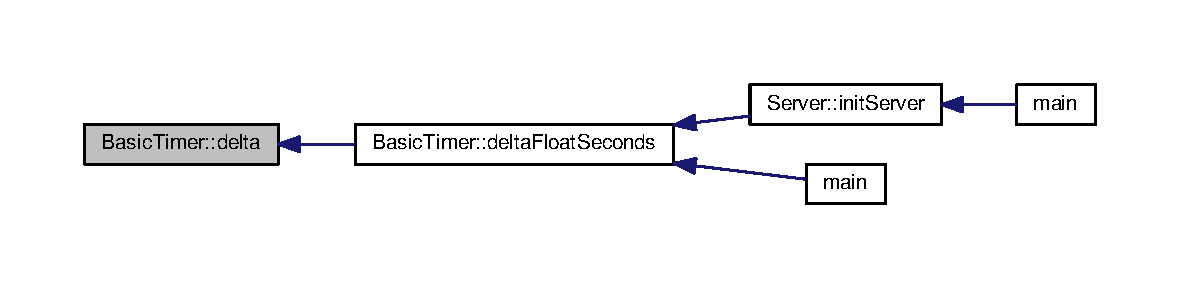
\includegraphics[width=350pt]{class_basic_timer_a49bc91a549323a1a7fc6b7d9ec727174_icgraph}
\end{center}
\end{figure}


\hypertarget{class_basic_timer_afbe3d01b15f26573eb12c04ae7c28684}{\index{Basic\-Timer@{Basic\-Timer}!delta\-Float\-Seconds@{delta\-Float\-Seconds}}
\index{delta\-Float\-Seconds@{delta\-Float\-Seconds}!BasicTimer@{Basic\-Timer}}
\subsubsection[{delta\-Float\-Seconds}]{\setlength{\rightskip}{0pt plus 5cm}double Basic\-Timer\-::delta\-Float\-Seconds (
\begin{DoxyParamCaption}
{}
\end{DoxyParamCaption}
) const\hspace{0.3cm}{\ttfamily [virtual]}}}\label{class_basic_timer_afbe3d01b15f26573eb12c04ae7c28684}
\begin{DoxyReturn}{Returns}
Time from last update in float-\/number seconds. 
\end{DoxyReturn}


Implements \hyperlink{class_i_timer_a495a1de5043065f9097c5d3a8b32998a}{I\-Timer}.



Here is the call graph for this function\-:
\nopagebreak
\begin{figure}[H]
\begin{center}
\leavevmode
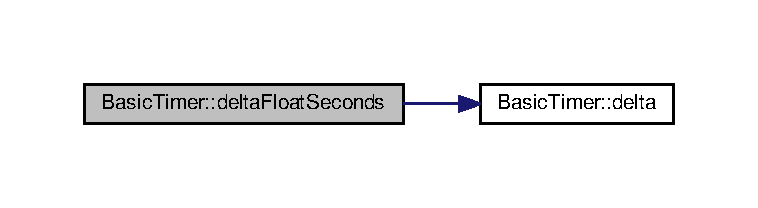
\includegraphics[width=350pt]{class_basic_timer_afbe3d01b15f26573eb12c04ae7c28684_cgraph}
\end{center}
\end{figure}




Here is the caller graph for this function\-:
\nopagebreak
\begin{figure}[H]
\begin{center}
\leavevmode
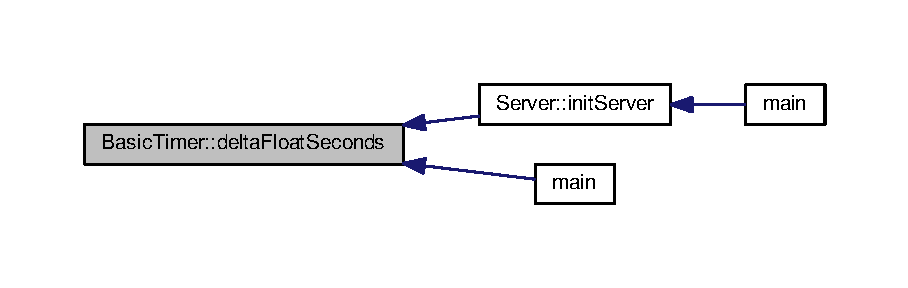
\includegraphics[width=308pt]{class_basic_timer_afbe3d01b15f26573eb12c04ae7c28684_icgraph}
\end{center}
\end{figure}


\hypertarget{class_basic_timer_abf76823ef1c782a0c6d49af2652b5271}{\index{Basic\-Timer@{Basic\-Timer}!update@{update}}
\index{update@{update}!BasicTimer@{Basic\-Timer}}
\subsubsection[{update}]{\setlength{\rightskip}{0pt plus 5cm}void Basic\-Timer\-::update (
\begin{DoxyParamCaption}
{}
\end{DoxyParamCaption}
)\hspace{0.3cm}{\ttfamily [virtual]}}}\label{class_basic_timer_abf76823ef1c782a0c6d49af2652b5271}
Saves update, saves the \char`\"{}tick\char`\"{}. It will influence value of {\ttfamily delta}. 

Implements \hyperlink{class_i_timer_afa6c0d962817423715ce9f944f1b6a2c}{I\-Timer}.



Here is the caller graph for this function\-:
\nopagebreak
\begin{figure}[H]
\begin{center}
\leavevmode
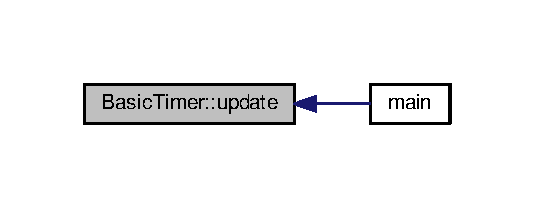
\includegraphics[width=256pt]{class_basic_timer_abf76823ef1c782a0c6d49af2652b5271_icgraph}
\end{center}
\end{figure}




\subsection{Member Data Documentation}
\hypertarget{class_basic_timer_a1c5ab332f195b367d5fbf91183f4dc8a}{\index{Basic\-Timer@{Basic\-Timer}!\-\_\-last\-Update\-Time@{\-\_\-last\-Update\-Time}}
\index{\-\_\-last\-Update\-Time@{\-\_\-last\-Update\-Time}!BasicTimer@{Basic\-Timer}}
\subsubsection[{\-\_\-last\-Update\-Time}]{\setlength{\rightskip}{0pt plus 5cm}std\-::chrono\-::system\-\_\-clock\-::time\-\_\-point Basic\-Timer\-::\-\_\-last\-Update\-Time\hspace{0.3cm}{\ttfamily [protected]}}}\label{class_basic_timer_a1c5ab332f195b367d5fbf91183f4dc8a}


The documentation for this class was generated from the following files\-:\begin{DoxyCompactItemize}
\item 
/home/travis/build/bender-\/wardrobe/\-Recast/temperature-\/world/src/headers/temperature-\/world/implementation/\hyperlink{_basic_timer_8hpp}{Basic\-Timer.\-hpp}\item 
/home/travis/build/bender-\/wardrobe/\-Recast/temperature-\/world/src/implementation/\hyperlink{_basic_timer_8cpp}{Basic\-Timer.\-cpp}\end{DoxyCompactItemize}

\hypertarget{class_bound_temperature_world}{\section{Bound\-Temperature\-World Class Reference}
\label{class_bound_temperature_world}\index{Bound\-Temperature\-World@{Bound\-Temperature\-World}}
}


{\ttfamily \#include $<$Bound\-Temperature\-World.\-hpp$>$}



Inheritance diagram for Bound\-Temperature\-World\-:
\nopagebreak
\begin{figure}[H]
\begin{center}
\leavevmode
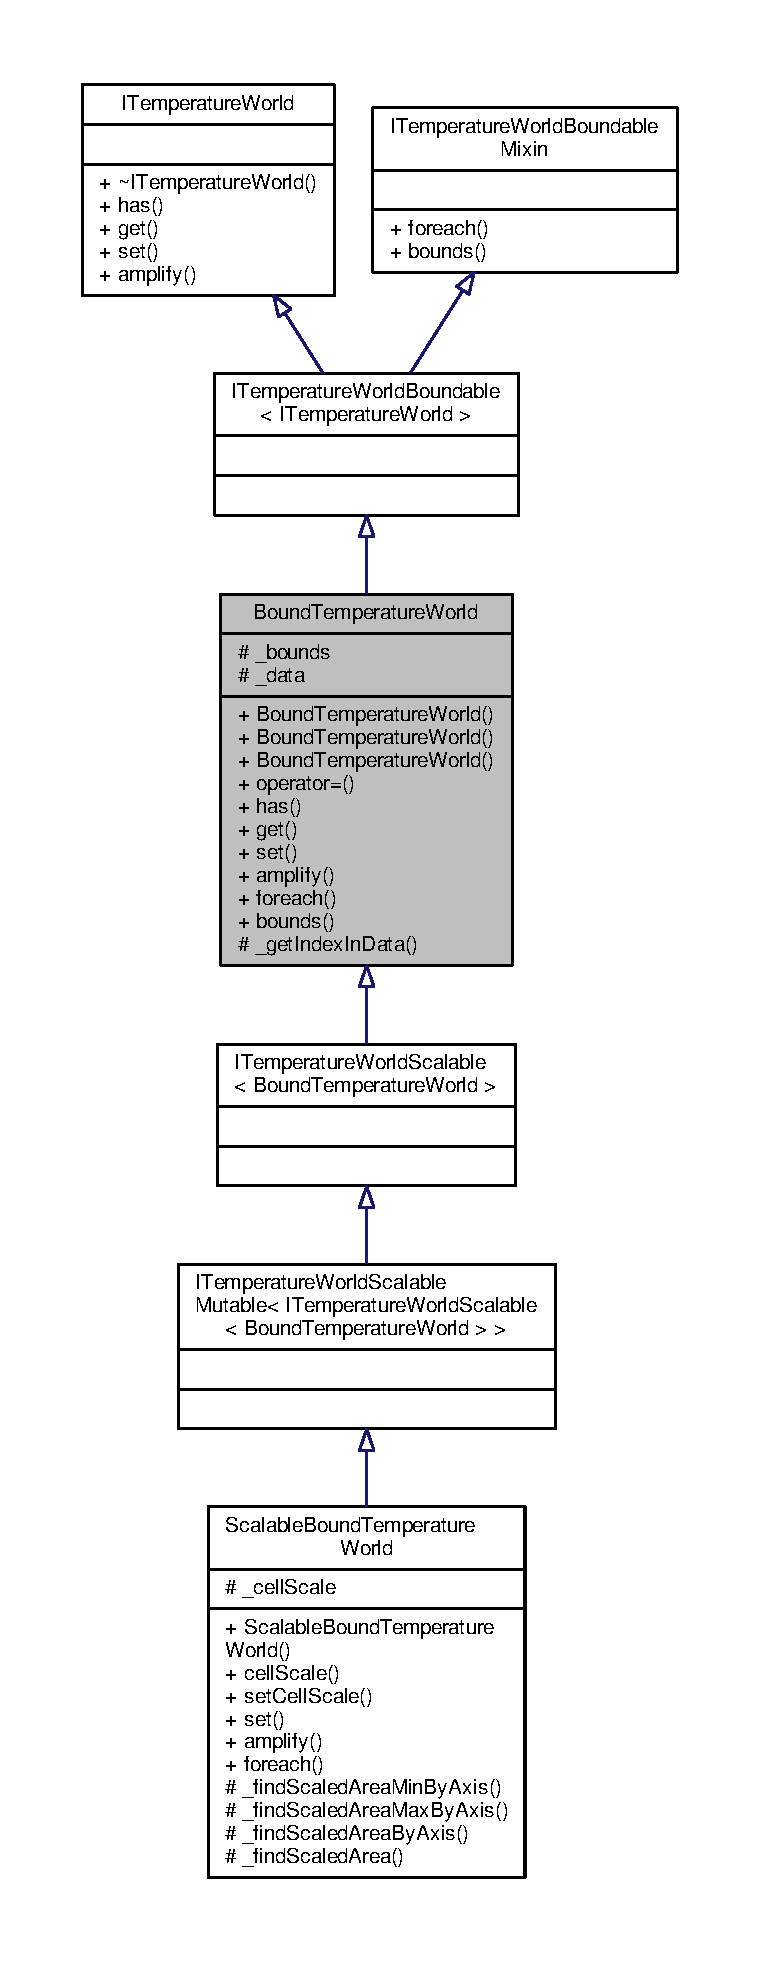
\includegraphics[height=550pt]{class_bound_temperature_world__inherit__graph}
\end{center}
\end{figure}


Collaboration diagram for Bound\-Temperature\-World\-:
\nopagebreak
\begin{figure}[H]
\begin{center}
\leavevmode
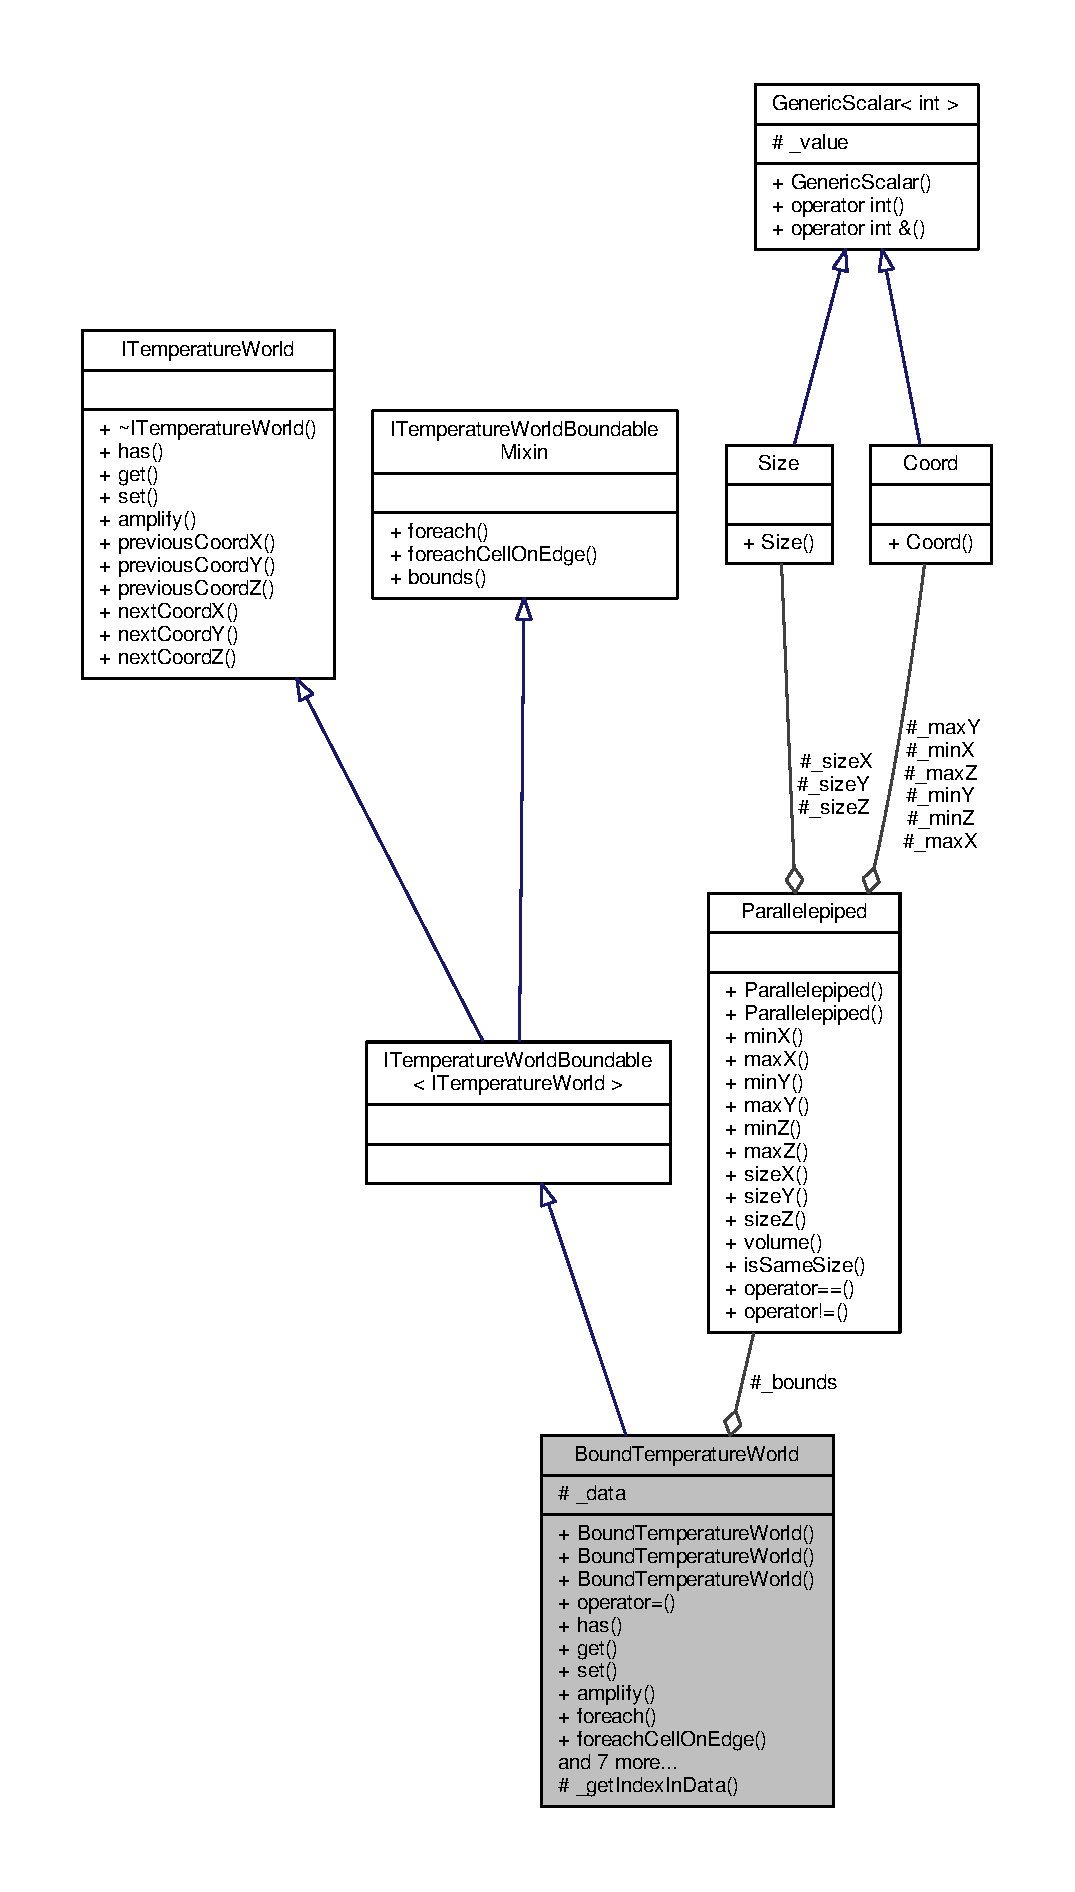
\includegraphics[height=550pt]{class_bound_temperature_world__coll__graph}
\end{center}
\end{figure}
\subsection*{Public Member Functions}
\begin{DoxyCompactItemize}
\item 
\hyperlink{class_bound_temperature_world_ab1843b429dc37c0c09ef0b454b9ea908}{Bound\-Temperature\-World} (\hyperlink{struct_parallelepiped}{Parallelepiped} \hyperlink{class_bound_temperature_world_a3351693a7d184365da5dfb5d833a0cb6}{bounds})
\item 
\hyperlink{class_bound_temperature_world_ae022092cb3feca841a569a1be7ab650a}{Bound\-Temperature\-World} (const \hyperlink{class_bound_temperature_world}{Bound\-Temperature\-World} \&other)
\item 
\hyperlink{class_bound_temperature_world_ae8406206a559d955ce53d18f4e2ec45b}{Bound\-Temperature\-World} (\hyperlink{class_bound_temperature_world}{Bound\-Temperature\-World} \&\&other)
\item 
\hyperlink{class_bound_temperature_world}{Bound\-Temperature\-World} \& \hyperlink{class_bound_temperature_world_a0501d4803249b0724ee87cd125f81481}{operator=} (\hyperlink{class_bound_temperature_world}{Bound\-Temperature\-World} other)
\item 
bool \hyperlink{class_bound_temperature_world_a75d2d3c631fb355de63dea3961ecd32b}{has} (\hyperlink{struct_coord}{Coord} x, \hyperlink{struct_coord}{Coord} y, \hyperlink{struct_coord}{Coord} z) const noexceptoverride
\item 
\hyperlink{struct_temperature}{Temperature} \hyperlink{class_bound_temperature_world_a1a668e9632e4179029cabad5052428fc}{get} (\hyperlink{struct_coord}{Coord} x, \hyperlink{struct_coord}{Coord} y, \hyperlink{struct_coord}{Coord} z) const override
\item 
void \hyperlink{class_bound_temperature_world_aa069691f31dd38006cfeacab94b6e94e}{set} (\hyperlink{struct_coord}{Coord} x, \hyperlink{struct_coord}{Coord} y, \hyperlink{struct_coord}{Coord} z, \hyperlink{struct_temperature}{Temperature} temperature) override
\item 
void \hyperlink{class_bound_temperature_world_a7b49bd6e07cc78f3c7a3a722d0ec5bac}{amplify} (\hyperlink{struct_coord}{Coord} x, \hyperlink{struct_coord}{Coord} y, \hyperlink{struct_coord}{Coord} z, \hyperlink{struct_temperature}{Temperature} temperature) override
\item 
void \hyperlink{class_bound_temperature_world_afac2a24af176488487ef7aaa62936ee7}{foreach} (\hyperlink{class_i_temperature_world_boundable_mixin_a370c20d79642d15e97843da972d87ba9}{Foreach\-Cell\-Fn} func) const override
\item 
\hyperlink{struct_parallelepiped}{Parallelepiped} \hyperlink{class_bound_temperature_world_a3351693a7d184365da5dfb5d833a0cb6}{bounds} () const noexceptoverride
\end{DoxyCompactItemize}
\subsection*{Protected Member Functions}
\begin{DoxyCompactItemize}
\item 
virtual size\-\_\-t \hyperlink{class_bound_temperature_world_a6be6a48b1a29f0b1cc4a01b5e0369f9e}{\-\_\-get\-Index\-In\-Data} (\hyperlink{struct_coord}{Coord} x, \hyperlink{struct_coord}{Coord} y, \hyperlink{struct_coord}{Coord} z) const 
\end{DoxyCompactItemize}
\subsection*{Protected Attributes}
\begin{DoxyCompactItemize}
\item 
\hyperlink{struct_parallelepiped}{Parallelepiped} \hyperlink{class_bound_temperature_world_a4e460fde774b68cb821e6b263e71448b}{\-\_\-bounds}
\item 
std\-::vector$<$ \hyperlink{struct_temperature}{Temperature} $>$ \hyperlink{class_bound_temperature_world_a7c0722e68bbe02de068ccb6244522c7a}{\-\_\-data}
\end{DoxyCompactItemize}
\subsection*{Friends}
\begin{DoxyCompactItemize}
\item 
void \hyperlink{class_bound_temperature_world_a684a1f2310369a9bcf86e6c8e4384e51}{swap} (\hyperlink{class_bound_temperature_world}{Bound\-Temperature\-World} \&first, \hyperlink{class_bound_temperature_world}{Bound\-Temperature\-World} \&second)
\end{DoxyCompactItemize}
\subsection*{Additional Inherited Members}


\subsection{Detailed Description}
Implementation of temperature world with bounds. It's backed by {\ttfamily std\-::vector}. 

\subsection{Constructor \& Destructor Documentation}
\hypertarget{class_bound_temperature_world_ab1843b429dc37c0c09ef0b454b9ea908}{\index{Bound\-Temperature\-World@{Bound\-Temperature\-World}!Bound\-Temperature\-World@{Bound\-Temperature\-World}}
\index{Bound\-Temperature\-World@{Bound\-Temperature\-World}!BoundTemperatureWorld@{Bound\-Temperature\-World}}
\subsubsection[{Bound\-Temperature\-World}]{\setlength{\rightskip}{0pt plus 5cm}Bound\-Temperature\-World\-::\-Bound\-Temperature\-World (
\begin{DoxyParamCaption}
\item[{{\bf Parallelepiped}}]{bounds}
\end{DoxyParamCaption}
)}}\label{class_bound_temperature_world_ab1843b429dc37c0c09ef0b454b9ea908}


Here is the call graph for this function\-:
\nopagebreak
\begin{figure}[H]
\begin{center}
\leavevmode
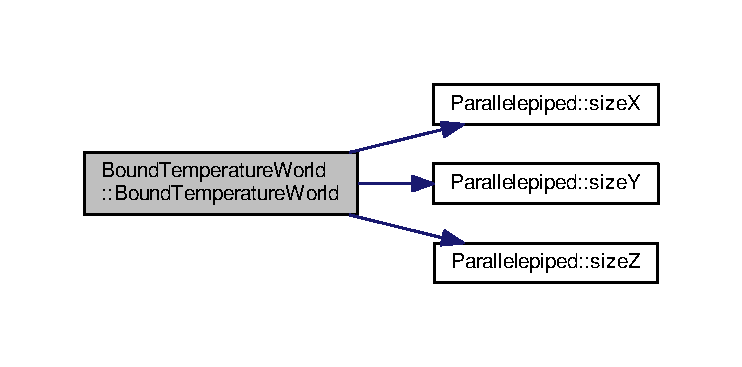
\includegraphics[width=350pt]{class_bound_temperature_world_ab1843b429dc37c0c09ef0b454b9ea908_cgraph}
\end{center}
\end{figure}


\hypertarget{class_bound_temperature_world_ae022092cb3feca841a569a1be7ab650a}{\index{Bound\-Temperature\-World@{Bound\-Temperature\-World}!Bound\-Temperature\-World@{Bound\-Temperature\-World}}
\index{Bound\-Temperature\-World@{Bound\-Temperature\-World}!BoundTemperatureWorld@{Bound\-Temperature\-World}}
\subsubsection[{Bound\-Temperature\-World}]{\setlength{\rightskip}{0pt plus 5cm}Bound\-Temperature\-World\-::\-Bound\-Temperature\-World (
\begin{DoxyParamCaption}
\item[{const {\bf Bound\-Temperature\-World} \&}]{other}
\end{DoxyParamCaption}
)}}\label{class_bound_temperature_world_ae022092cb3feca841a569a1be7ab650a}
\hypertarget{class_bound_temperature_world_ae8406206a559d955ce53d18f4e2ec45b}{\index{Bound\-Temperature\-World@{Bound\-Temperature\-World}!Bound\-Temperature\-World@{Bound\-Temperature\-World}}
\index{Bound\-Temperature\-World@{Bound\-Temperature\-World}!BoundTemperatureWorld@{Bound\-Temperature\-World}}
\subsubsection[{Bound\-Temperature\-World}]{\setlength{\rightskip}{0pt plus 5cm}Bound\-Temperature\-World\-::\-Bound\-Temperature\-World (
\begin{DoxyParamCaption}
\item[{{\bf Bound\-Temperature\-World} \&\&}]{other}
\end{DoxyParamCaption}
)}}\label{class_bound_temperature_world_ae8406206a559d955ce53d18f4e2ec45b}


\subsection{Member Function Documentation}
\hypertarget{class_bound_temperature_world_a6be6a48b1a29f0b1cc4a01b5e0369f9e}{\index{Bound\-Temperature\-World@{Bound\-Temperature\-World}!\-\_\-get\-Index\-In\-Data@{\-\_\-get\-Index\-In\-Data}}
\index{\-\_\-get\-Index\-In\-Data@{\-\_\-get\-Index\-In\-Data}!BoundTemperatureWorld@{Bound\-Temperature\-World}}
\subsubsection[{\-\_\-get\-Index\-In\-Data}]{\setlength{\rightskip}{0pt plus 5cm}size\-\_\-t Bound\-Temperature\-World\-::\-\_\-get\-Index\-In\-Data (
\begin{DoxyParamCaption}
\item[{{\bf Coord}}]{x, }
\item[{{\bf Coord}}]{y, }
\item[{{\bf Coord}}]{z}
\end{DoxyParamCaption}
) const\hspace{0.3cm}{\ttfamily [protected]}, {\ttfamily [virtual]}}}\label{class_bound_temperature_world_a6be6a48b1a29f0b1cc4a01b5e0369f9e}


Here is the call graph for this function\-:
\nopagebreak
\begin{figure}[H]
\begin{center}
\leavevmode
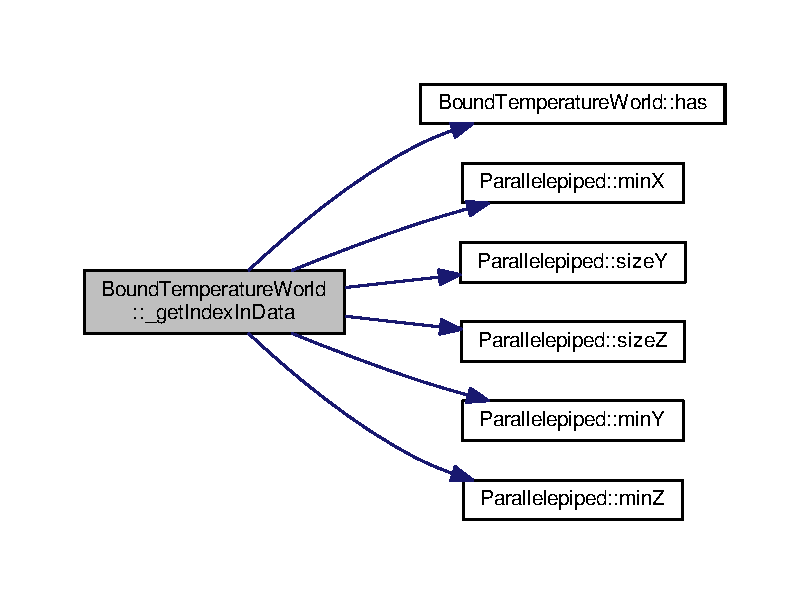
\includegraphics[width=350pt]{class_bound_temperature_world_a6be6a48b1a29f0b1cc4a01b5e0369f9e_cgraph}
\end{center}
\end{figure}




Here is the caller graph for this function\-:
\nopagebreak
\begin{figure}[H]
\begin{center}
\leavevmode
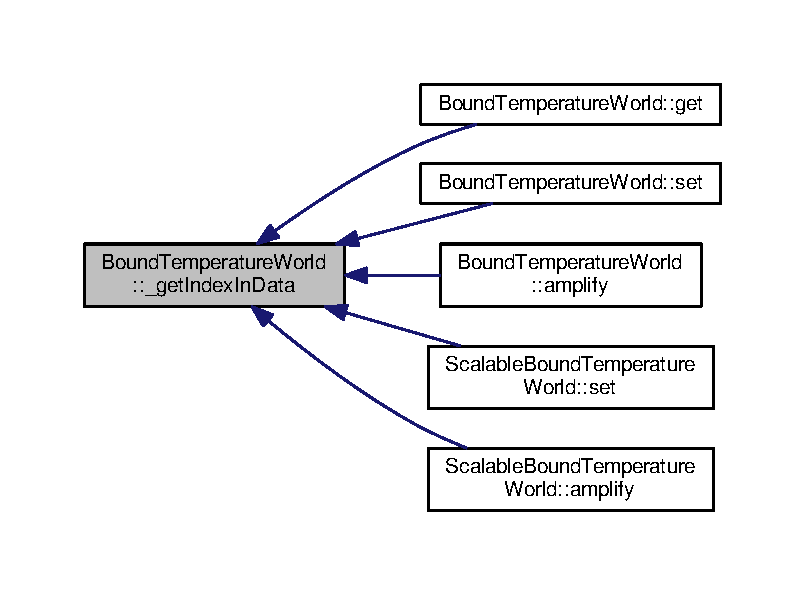
\includegraphics[width=350pt]{class_bound_temperature_world_a6be6a48b1a29f0b1cc4a01b5e0369f9e_icgraph}
\end{center}
\end{figure}


\hypertarget{class_bound_temperature_world_a7b49bd6e07cc78f3c7a3a722d0ec5bac}{\index{Bound\-Temperature\-World@{Bound\-Temperature\-World}!amplify@{amplify}}
\index{amplify@{amplify}!BoundTemperatureWorld@{Bound\-Temperature\-World}}
\subsubsection[{amplify}]{\setlength{\rightskip}{0pt plus 5cm}void Bound\-Temperature\-World\-::amplify (
\begin{DoxyParamCaption}
\item[{{\bf Coord}}]{x, }
\item[{{\bf Coord}}]{y, }
\item[{{\bf Coord}}]{z, }
\item[{{\bf Temperature}}]{temperature}
\end{DoxyParamCaption}
)\hspace{0.3cm}{\ttfamily [override]}, {\ttfamily [virtual]}}}\label{class_bound_temperature_world_a7b49bd6e07cc78f3c7a3a722d0ec5bac}
Adds or substracts temperature value from existing temperature value at the point.


\begin{DoxyParams}{Parameters}
{\em x} & X coordinate. \\
\hline
{\em y} & Y coordinate. \\
\hline
{\em z} & Z coordinate. \\
\hline
{\em temperature} & \hyperlink{struct_temperature}{Temperature} difference. \\
\hline
\end{DoxyParams}


Implements \hyperlink{class_i_temperature_world_ac5a8a92e7141b2e2c2e3d66ba73b7c1e}{I\-Temperature\-World}.



Reimplemented in \hyperlink{class_scalable_bound_temperature_world_ab9602b36759aa857910e03856344759d}{Scalable\-Bound\-Temperature\-World}.



Here is the call graph for this function\-:
\nopagebreak
\begin{figure}[H]
\begin{center}
\leavevmode
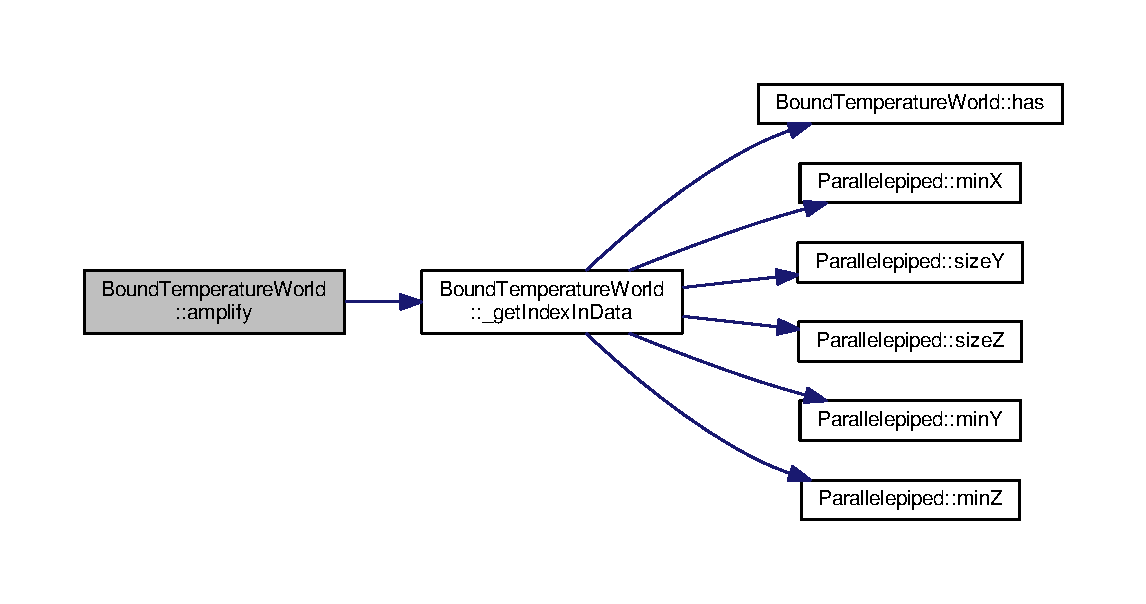
\includegraphics[width=350pt]{class_bound_temperature_world_a7b49bd6e07cc78f3c7a3a722d0ec5bac_cgraph}
\end{center}
\end{figure}




Here is the caller graph for this function\-:
\nopagebreak
\begin{figure}[H]
\begin{center}
\leavevmode
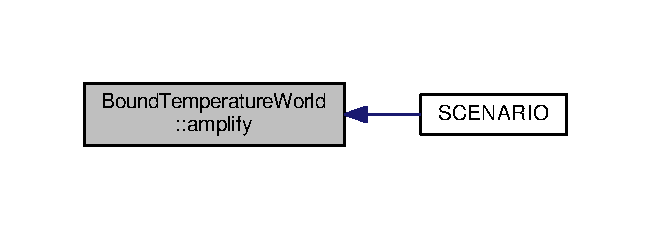
\includegraphics[width=312pt]{class_bound_temperature_world_a7b49bd6e07cc78f3c7a3a722d0ec5bac_icgraph}
\end{center}
\end{figure}


\hypertarget{class_bound_temperature_world_a3351693a7d184365da5dfb5d833a0cb6}{\index{Bound\-Temperature\-World@{Bound\-Temperature\-World}!bounds@{bounds}}
\index{bounds@{bounds}!BoundTemperatureWorld@{Bound\-Temperature\-World}}
\subsubsection[{bounds}]{\setlength{\rightskip}{0pt plus 5cm}{\bf Parallelepiped} Bound\-Temperature\-World\-::bounds (
\begin{DoxyParamCaption}
{}
\end{DoxyParamCaption}
) const\hspace{0.3cm}{\ttfamily [override]}, {\ttfamily [virtual]}, {\ttfamily [noexcept]}}}\label{class_bound_temperature_world_a3351693a7d184365da5dfb5d833a0cb6}
\begin{DoxyReturn}{Returns}
Bounds of this temperature world. 
\end{DoxyReturn}


Implements \hyperlink{class_i_temperature_world_boundable_mixin_a4811acd7f2bade56752c6326b0860f0c}{I\-Temperature\-World\-Boundable\-Mixin}.



Here is the caller graph for this function\-:
\nopagebreak
\begin{figure}[H]
\begin{center}
\leavevmode
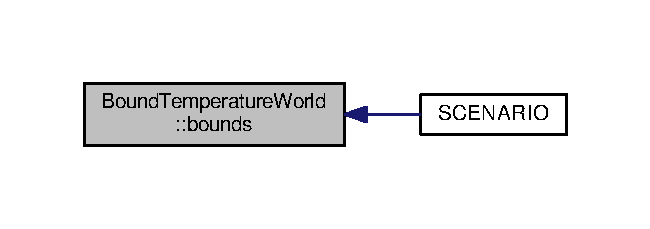
\includegraphics[width=312pt]{class_bound_temperature_world_a3351693a7d184365da5dfb5d833a0cb6_icgraph}
\end{center}
\end{figure}


\hypertarget{class_bound_temperature_world_afac2a24af176488487ef7aaa62936ee7}{\index{Bound\-Temperature\-World@{Bound\-Temperature\-World}!foreach@{foreach}}
\index{foreach@{foreach}!BoundTemperatureWorld@{Bound\-Temperature\-World}}
\subsubsection[{foreach}]{\setlength{\rightskip}{0pt plus 5cm}void Bound\-Temperature\-World\-::foreach (
\begin{DoxyParamCaption}
\item[{{\bf Foreach\-Cell\-Fn}}]{func}
\end{DoxyParamCaption}
) const\hspace{0.3cm}{\ttfamily [override]}, {\ttfamily [virtual]}}}\label{class_bound_temperature_world_afac2a24af176488487ef7aaa62936ee7}
Loops over each point.


\begin{DoxyParams}{Parameters}
{\em func} & Function to execute at each point. \\
\hline
\end{DoxyParams}


Implements \hyperlink{class_i_temperature_world_boundable_mixin_ac350b2e2ea22a229e6543d55e3217317}{I\-Temperature\-World\-Boundable\-Mixin}.



Reimplemented in \hyperlink{class_scalable_bound_temperature_world_a57f60178c88b2cffca11a7f21c5c11c7}{Scalable\-Bound\-Temperature\-World}.



Here is the call graph for this function\-:
\nopagebreak
\begin{figure}[H]
\begin{center}
\leavevmode
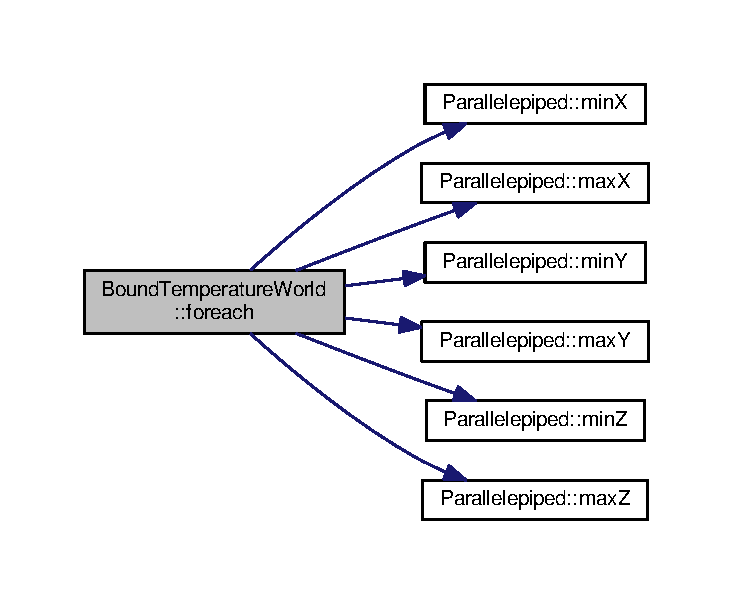
\includegraphics[width=350pt]{class_bound_temperature_world_afac2a24af176488487ef7aaa62936ee7_cgraph}
\end{center}
\end{figure}


\hypertarget{class_bound_temperature_world_a1a668e9632e4179029cabad5052428fc}{\index{Bound\-Temperature\-World@{Bound\-Temperature\-World}!get@{get}}
\index{get@{get}!BoundTemperatureWorld@{Bound\-Temperature\-World}}
\subsubsection[{get}]{\setlength{\rightskip}{0pt plus 5cm}{\bf Temperature} Bound\-Temperature\-World\-::get (
\begin{DoxyParamCaption}
\item[{{\bf Coord}}]{x, }
\item[{{\bf Coord}}]{y, }
\item[{{\bf Coord}}]{z}
\end{DoxyParamCaption}
) const\hspace{0.3cm}{\ttfamily [override]}, {\ttfamily [virtual]}}}\label{class_bound_temperature_world_a1a668e9632e4179029cabad5052428fc}
Returns temperature at the point.


\begin{DoxyParams}{Parameters}
{\em x} & X coordinate. \\
\hline
{\em y} & Y coordinate. \\
\hline
{\em z} & Z coordinate. \\
\hline
\end{DoxyParams}
\begin{DoxyReturn}{Returns}
\hyperlink{struct_temperature}{Temperature} at the point. 
\end{DoxyReturn}


Implements \hyperlink{class_i_temperature_world_a9993df60754c2c89597bd8137568c12f}{I\-Temperature\-World}.



Here is the call graph for this function\-:
\nopagebreak
\begin{figure}[H]
\begin{center}
\leavevmode
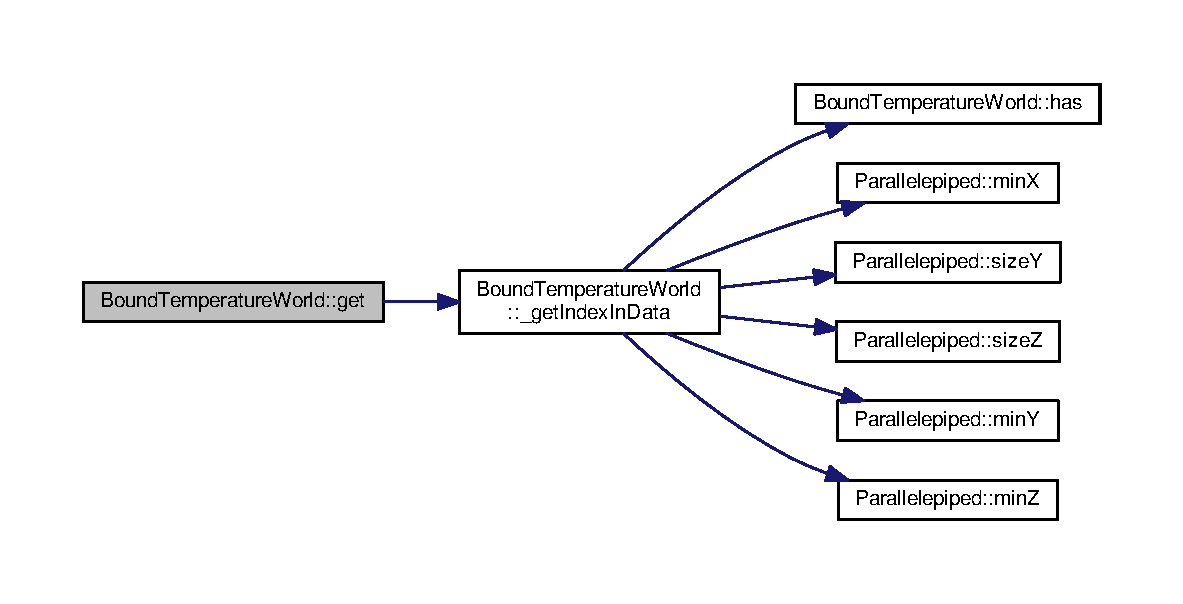
\includegraphics[width=350pt]{class_bound_temperature_world_a1a668e9632e4179029cabad5052428fc_cgraph}
\end{center}
\end{figure}




Here is the caller graph for this function\-:
\nopagebreak
\begin{figure}[H]
\begin{center}
\leavevmode
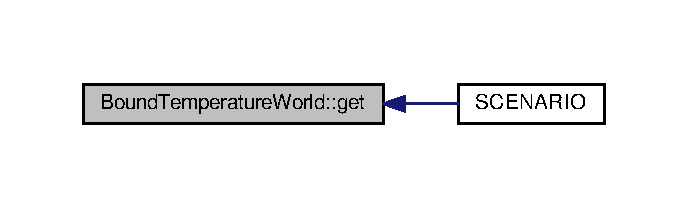
\includegraphics[width=330pt]{class_bound_temperature_world_a1a668e9632e4179029cabad5052428fc_icgraph}
\end{center}
\end{figure}


\hypertarget{class_bound_temperature_world_a75d2d3c631fb355de63dea3961ecd32b}{\index{Bound\-Temperature\-World@{Bound\-Temperature\-World}!has@{has}}
\index{has@{has}!BoundTemperatureWorld@{Bound\-Temperature\-World}}
\subsubsection[{has}]{\setlength{\rightskip}{0pt plus 5cm}bool Bound\-Temperature\-World\-::has (
\begin{DoxyParamCaption}
\item[{{\bf Coord}}]{x, }
\item[{{\bf Coord}}]{y, }
\item[{{\bf Coord}}]{z}
\end{DoxyParamCaption}
) const\hspace{0.3cm}{\ttfamily [override]}, {\ttfamily [virtual]}, {\ttfamily [noexcept]}}}\label{class_bound_temperature_world_a75d2d3c631fb355de63dea3961ecd32b}
Tells whether temperature at the point is accessible. This method doesn't throw exceptions.


\begin{DoxyParams}{Parameters}
{\em x} & X coordinate. \\
\hline
{\em y} & Y coordinate. \\
\hline
{\em z} & Z coordinate. \\
\hline
\end{DoxyParams}
\begin{DoxyReturn}{Returns}
True if the point is accessible. 
\end{DoxyReturn}


Implements \hyperlink{class_i_temperature_world_a6c498247ed71d9ad037dd0c1b4779f81}{I\-Temperature\-World}.



Here is the caller graph for this function\-:
\nopagebreak
\begin{figure}[H]
\begin{center}
\leavevmode
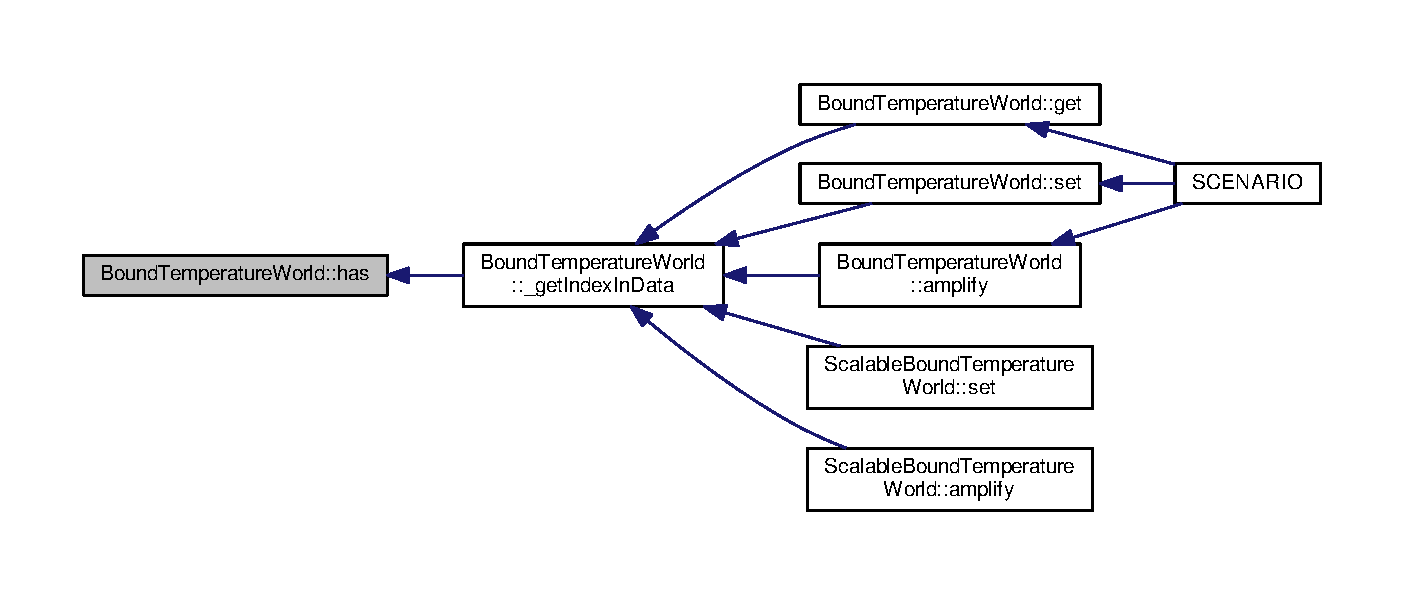
\includegraphics[width=350pt]{class_bound_temperature_world_a75d2d3c631fb355de63dea3961ecd32b_icgraph}
\end{center}
\end{figure}


\hypertarget{class_bound_temperature_world_a0501d4803249b0724ee87cd125f81481}{\index{Bound\-Temperature\-World@{Bound\-Temperature\-World}!operator=@{operator=}}
\index{operator=@{operator=}!BoundTemperatureWorld@{Bound\-Temperature\-World}}
\subsubsection[{operator=}]{\setlength{\rightskip}{0pt plus 5cm}{\bf Bound\-Temperature\-World} \& Bound\-Temperature\-World\-::operator= (
\begin{DoxyParamCaption}
\item[{{\bf Bound\-Temperature\-World}}]{other}
\end{DoxyParamCaption}
)}}\label{class_bound_temperature_world_a0501d4803249b0724ee87cd125f81481}
\hypertarget{class_bound_temperature_world_aa069691f31dd38006cfeacab94b6e94e}{\index{Bound\-Temperature\-World@{Bound\-Temperature\-World}!set@{set}}
\index{set@{set}!BoundTemperatureWorld@{Bound\-Temperature\-World}}
\subsubsection[{set}]{\setlength{\rightskip}{0pt plus 5cm}void Bound\-Temperature\-World\-::set (
\begin{DoxyParamCaption}
\item[{{\bf Coord}}]{x, }
\item[{{\bf Coord}}]{y, }
\item[{{\bf Coord}}]{z, }
\item[{{\bf Temperature}}]{temperature}
\end{DoxyParamCaption}
)\hspace{0.3cm}{\ttfamily [override]}, {\ttfamily [virtual]}}}\label{class_bound_temperature_world_aa069691f31dd38006cfeacab94b6e94e}
Sets temperature at the point.


\begin{DoxyParams}{Parameters}
{\em x} & X coordinate. \\
\hline
{\em y} & Y coordinate. \\
\hline
{\em z} & Z coordinate. \\
\hline
{\em temperature} & \hyperlink{struct_temperature}{Temperature} to set. \\
\hline
\end{DoxyParams}


Implements \hyperlink{class_i_temperature_world_ab23db7ec9a890d6dbb172b26c2fd3d00}{I\-Temperature\-World}.



Reimplemented in \hyperlink{class_scalable_bound_temperature_world_ade4ecf303ae025e824c0bd5ecd2e2ca7}{Scalable\-Bound\-Temperature\-World}.



Here is the call graph for this function\-:
\nopagebreak
\begin{figure}[H]
\begin{center}
\leavevmode
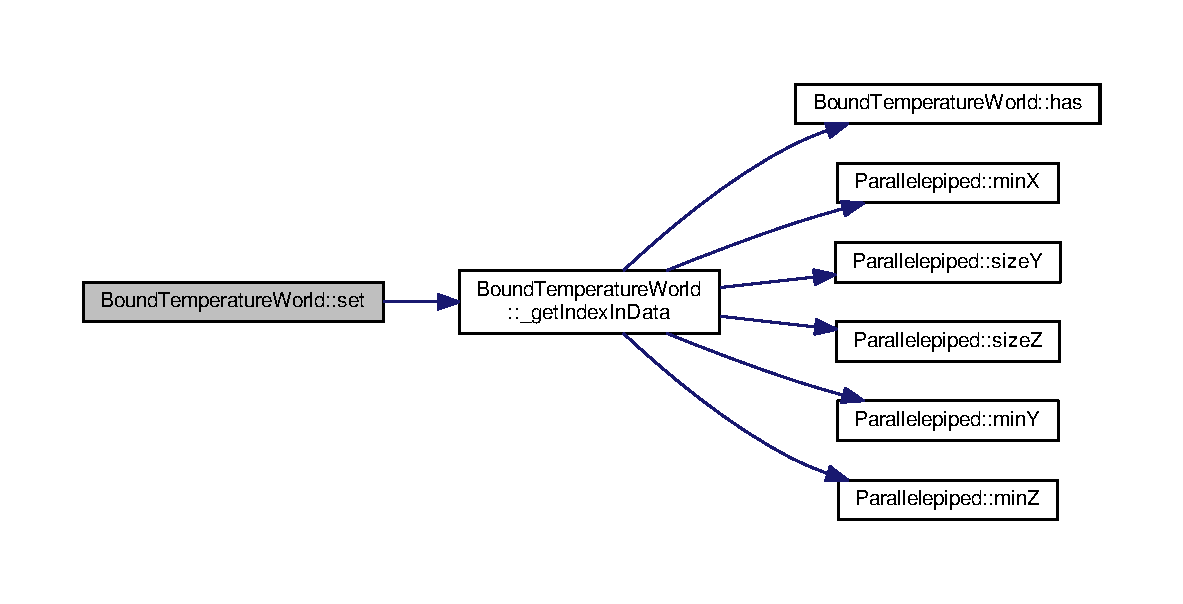
\includegraphics[width=350pt]{class_bound_temperature_world_aa069691f31dd38006cfeacab94b6e94e_cgraph}
\end{center}
\end{figure}




Here is the caller graph for this function\-:
\nopagebreak
\begin{figure}[H]
\begin{center}
\leavevmode
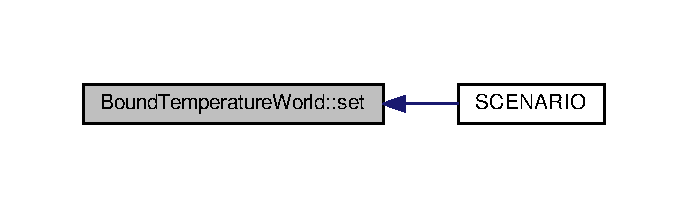
\includegraphics[width=330pt]{class_bound_temperature_world_aa069691f31dd38006cfeacab94b6e94e_icgraph}
\end{center}
\end{figure}




\subsection{Friends And Related Function Documentation}
\hypertarget{class_bound_temperature_world_a684a1f2310369a9bcf86e6c8e4384e51}{\index{Bound\-Temperature\-World@{Bound\-Temperature\-World}!swap@{swap}}
\index{swap@{swap}!BoundTemperatureWorld@{Bound\-Temperature\-World}}
\subsubsection[{swap}]{\setlength{\rightskip}{0pt plus 5cm}void swap (
\begin{DoxyParamCaption}
\item[{{\bf Bound\-Temperature\-World} \&}]{first, }
\item[{{\bf Bound\-Temperature\-World} \&}]{second}
\end{DoxyParamCaption}
)\hspace{0.3cm}{\ttfamily [friend]}}}\label{class_bound_temperature_world_a684a1f2310369a9bcf86e6c8e4384e51}


\subsection{Member Data Documentation}
\hypertarget{class_bound_temperature_world_a4e460fde774b68cb821e6b263e71448b}{\index{Bound\-Temperature\-World@{Bound\-Temperature\-World}!\-\_\-bounds@{\-\_\-bounds}}
\index{\-\_\-bounds@{\-\_\-bounds}!BoundTemperatureWorld@{Bound\-Temperature\-World}}
\subsubsection[{\-\_\-bounds}]{\setlength{\rightskip}{0pt plus 5cm}{\bf Parallelepiped} Bound\-Temperature\-World\-::\-\_\-bounds\hspace{0.3cm}{\ttfamily [protected]}}}\label{class_bound_temperature_world_a4e460fde774b68cb821e6b263e71448b}
\hypertarget{class_bound_temperature_world_a7c0722e68bbe02de068ccb6244522c7a}{\index{Bound\-Temperature\-World@{Bound\-Temperature\-World}!\-\_\-data@{\-\_\-data}}
\index{\-\_\-data@{\-\_\-data}!BoundTemperatureWorld@{Bound\-Temperature\-World}}
\subsubsection[{\-\_\-data}]{\setlength{\rightskip}{0pt plus 5cm}std\-::vector$<${\bf Temperature}$>$ Bound\-Temperature\-World\-::\-\_\-data\hspace{0.3cm}{\ttfamily [protected]}}}\label{class_bound_temperature_world_a7c0722e68bbe02de068ccb6244522c7a}


The documentation for this class was generated from the following files\-:\begin{DoxyCompactItemize}
\item 
/home/travis/build/bender-\/wardrobe/\-Recast/temperature-\/world/src/headers/temperature-\/world/implementation/\hyperlink{_bound_temperature_world_8hpp}{Bound\-Temperature\-World.\-hpp}\item 
/home/travis/build/bender-\/wardrobe/\-Recast/temperature-\/world/src/implementation/\hyperlink{_bound_temperature_world_8cpp}{Bound\-Temperature\-World.\-cpp}\end{DoxyCompactItemize}

\hypertarget{class_bound_temperature_world_injector}{\section{Bound\-Temperature\-World\-Injector Class Reference}
\label{class_bound_temperature_world_injector}\index{Bound\-Temperature\-World\-Injector@{Bound\-Temperature\-World\-Injector}}
}


{\ttfamily \#include $<$Bound\-Temperature\-World\-Injector.\-hpp$>$}



Collaboration diagram for Bound\-Temperature\-World\-Injector\-:
\nopagebreak
\begin{figure}[H]
\begin{center}
\leavevmode
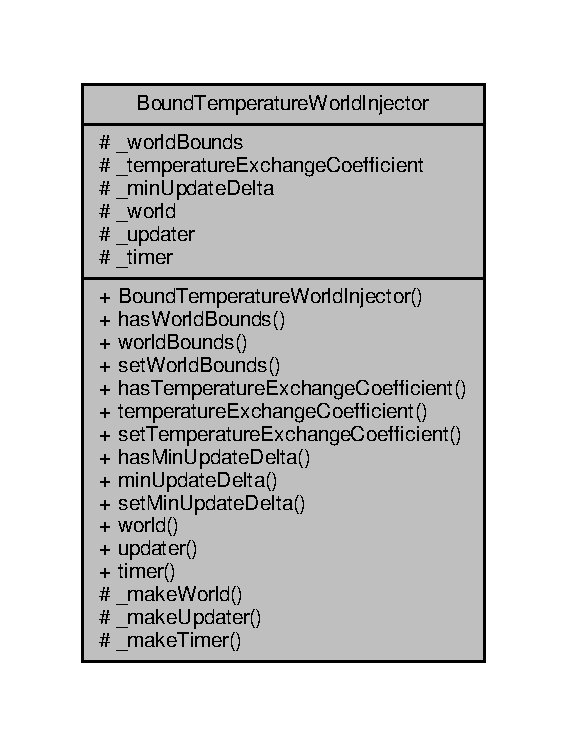
\includegraphics[width=272pt]{class_bound_temperature_world_injector__coll__graph}
\end{center}
\end{figure}
\subsection*{Public Member Functions}
\begin{DoxyCompactItemize}
\item 
\hyperlink{class_bound_temperature_world_injector_a8c9341a5ced28d934273c3fc265b1bf1}{Bound\-Temperature\-World\-Injector} ()
\item 
bool \hyperlink{class_bound_temperature_world_injector_a71c03ba809495eed2b09318343ded2d2}{has\-World\-Bounds} () const noexcept
\item 
\hyperlink{struct_parallelepiped}{Parallelepiped} \hyperlink{class_bound_temperature_world_injector_a33e6c7646ca32618e8d073fdaba33065}{world\-Bounds} () const 
\item 
void \hyperlink{class_bound_temperature_world_injector_aa3c6c0c782869509238b83774434347c}{set\-World\-Bounds} (\hyperlink{struct_parallelepiped}{Parallelepiped} \hyperlink{class_bound_temperature_world_injector_a33e6c7646ca32618e8d073fdaba33065}{world\-Bounds})
\item 
bool \hyperlink{class_bound_temperature_world_injector_a1274c81082b7ce2ce2bc433d7e93c17b}{has\-Temperature\-Exchange\-Coefficient} () const noexcept
\item 
double \hyperlink{class_bound_temperature_world_injector_a27e7b6a6da5015cadbbe7f21ad503287}{temperature\-Exchange\-Coefficient} () const 
\item 
void \hyperlink{class_bound_temperature_world_injector_a1e71c5d4a8397b9c8f87bccfe5cf5328}{set\-Temperature\-Exchange\-Coefficient} (double \hyperlink{class_bound_temperature_world_injector_a27e7b6a6da5015cadbbe7f21ad503287}{temperature\-Exchange\-Coefficient})
\item 
bool \hyperlink{class_bound_temperature_world_injector_a1a1a9e8c8ee2ef48cffbcdcbc2e947e5}{has\-Min\-Update\-Delta} () const noexcept
\item 
std\-::chrono\-::milliseconds \hyperlink{class_bound_temperature_world_injector_ad064e87615066662fe67ba8b41c44959}{min\-Update\-Delta} () const 
\item 
void \hyperlink{class_bound_temperature_world_injector_a3017672c819fd74e17fb79d69aa7beae}{set\-Min\-Update\-Delta} (std\-::chrono\-::milliseconds \hyperlink{class_bound_temperature_world_injector_ad064e87615066662fe67ba8b41c44959}{min\-Update\-Delta})
\item 
std\-::shared\-\_\-ptr\\*
$<$ \hyperlink{class_i_temperature_world_boundable}{I\-Temperature\-World\-Boundable}\\*
$<$ \hyperlink{class_i_temperature_world}{I\-Temperature\-World} $>$ $>$ \hyperlink{class_bound_temperature_world_injector_a94a6c343fa6f0a8aa7640ba4338de3e4}{world} ()
\item 
std\-::shared\-\_\-ptr$<$ \hyperlink{class_i_updater}{I\-Updater} $>$ \hyperlink{class_bound_temperature_world_injector_ab14750f84b51f9fc1b1a4d1c19b03c19}{updater} ()
\item 
std\-::shared\-\_\-ptr\\*
$<$ \hyperlink{class_i_timer_blockable}{I\-Timer\-Blockable}$<$ \hyperlink{class_i_timer}{I\-Timer} $>$ $>$ \hyperlink{class_bound_temperature_world_injector_a9e26e356da13bae69d852c5b44d14bee}{timer} ()
\end{DoxyCompactItemize}
\subsection*{Protected Member Functions}
\begin{DoxyCompactItemize}
\item 
void \hyperlink{class_bound_temperature_world_injector_a91a04f4aef416fdb0d2351d67073ca7d}{\-\_\-make\-World} ()
\item 
void \hyperlink{class_bound_temperature_world_injector_a1500a30682f3fdf02b79d48a6d493586}{\-\_\-make\-Updater} ()
\item 
void \hyperlink{class_bound_temperature_world_injector_a5d11cb09bec8a8b026b900601d6dce73}{\-\_\-make\-Timer} ()
\end{DoxyCompactItemize}
\subsection*{Protected Attributes}
\begin{DoxyCompactItemize}
\item 
std\-::unique\-\_\-ptr$<$ \hyperlink{struct_parallelepiped}{Parallelepiped} $>$ \hyperlink{class_bound_temperature_world_injector_a99e1aa88a9e38bddb58c22b030a126c3}{\-\_\-world\-Bounds}
\item 
std\-::unique\-\_\-ptr$<$ double $>$ \hyperlink{class_bound_temperature_world_injector_ab9a509b3b413ac1ac3825413c8d5d61f}{\-\_\-temperature\-Exchange\-Coefficient}
\item 
std\-::unique\-\_\-ptr\\*
$<$ std\-::chrono\-::milliseconds $>$ \hyperlink{class_bound_temperature_world_injector_a30845955fe87ca6cb33993e98b222aa4}{\-\_\-min\-Update\-Delta}
\item 
std\-::shared\-\_\-ptr\\*
$<$ \hyperlink{class_i_temperature_world_boundable}{I\-Temperature\-World\-Boundable}\\*
$<$ \hyperlink{class_i_temperature_world}{I\-Temperature\-World} $>$ $>$ \hyperlink{class_bound_temperature_world_injector_a5917901f6697587dd6dd05b3f1fd0549}{\-\_\-world}
\item 
std\-::shared\-\_\-ptr$<$ \hyperlink{class_i_updater}{I\-Updater} $>$ \hyperlink{class_bound_temperature_world_injector_a1e6c06b5c8ecafe011f27fa69072751e}{\-\_\-updater}
\item 
std\-::shared\-\_\-ptr\\*
$<$ \hyperlink{class_i_timer_blockable}{I\-Timer\-Blockable}$<$ \hyperlink{class_i_timer}{I\-Timer} $>$ $>$ \hyperlink{class_bound_temperature_world_injector_aabf0e33720ede845f154e57f7cd7edfb}{\-\_\-timer}
\end{DoxyCompactItemize}


\subsection{Detailed Description}
Injector. This class builds bound temperature world and its updater. You must set world bounds via {\ttfamily set\-World\-Bounds} method. \hyperlink{struct_temperature}{Temperature} exchange coefficient and minimum update delta are set to defaults. 

\subsection{Constructor \& Destructor Documentation}
\hypertarget{class_bound_temperature_world_injector_a8c9341a5ced28d934273c3fc265b1bf1}{\index{Bound\-Temperature\-World\-Injector@{Bound\-Temperature\-World\-Injector}!Bound\-Temperature\-World\-Injector@{Bound\-Temperature\-World\-Injector}}
\index{Bound\-Temperature\-World\-Injector@{Bound\-Temperature\-World\-Injector}!BoundTemperatureWorldInjector@{Bound\-Temperature\-World\-Injector}}
\subsubsection[{Bound\-Temperature\-World\-Injector}]{\setlength{\rightskip}{0pt plus 5cm}Bound\-Temperature\-World\-Injector\-::\-Bound\-Temperature\-World\-Injector (
\begin{DoxyParamCaption}
{}
\end{DoxyParamCaption}
)}}\label{class_bound_temperature_world_injector_a8c9341a5ced28d934273c3fc265b1bf1}


\subsection{Member Function Documentation}
\hypertarget{class_bound_temperature_world_injector_a5d11cb09bec8a8b026b900601d6dce73}{\index{Bound\-Temperature\-World\-Injector@{Bound\-Temperature\-World\-Injector}!\-\_\-make\-Timer@{\-\_\-make\-Timer}}
\index{\-\_\-make\-Timer@{\-\_\-make\-Timer}!BoundTemperatureWorldInjector@{Bound\-Temperature\-World\-Injector}}
\subsubsection[{\-\_\-make\-Timer}]{\setlength{\rightskip}{0pt plus 5cm}void Bound\-Temperature\-World\-Injector\-::\-\_\-make\-Timer (
\begin{DoxyParamCaption}
{}
\end{DoxyParamCaption}
)\hspace{0.3cm}{\ttfamily [protected]}}}\label{class_bound_temperature_world_injector_a5d11cb09bec8a8b026b900601d6dce73}
\hypertarget{class_bound_temperature_world_injector_a1500a30682f3fdf02b79d48a6d493586}{\index{Bound\-Temperature\-World\-Injector@{Bound\-Temperature\-World\-Injector}!\-\_\-make\-Updater@{\-\_\-make\-Updater}}
\index{\-\_\-make\-Updater@{\-\_\-make\-Updater}!BoundTemperatureWorldInjector@{Bound\-Temperature\-World\-Injector}}
\subsubsection[{\-\_\-make\-Updater}]{\setlength{\rightskip}{0pt plus 5cm}void Bound\-Temperature\-World\-Injector\-::\-\_\-make\-Updater (
\begin{DoxyParamCaption}
{}
\end{DoxyParamCaption}
)\hspace{0.3cm}{\ttfamily [protected]}}}\label{class_bound_temperature_world_injector_a1500a30682f3fdf02b79d48a6d493586}
\hypertarget{class_bound_temperature_world_injector_a91a04f4aef416fdb0d2351d67073ca7d}{\index{Bound\-Temperature\-World\-Injector@{Bound\-Temperature\-World\-Injector}!\-\_\-make\-World@{\-\_\-make\-World}}
\index{\-\_\-make\-World@{\-\_\-make\-World}!BoundTemperatureWorldInjector@{Bound\-Temperature\-World\-Injector}}
\subsubsection[{\-\_\-make\-World}]{\setlength{\rightskip}{0pt plus 5cm}void Bound\-Temperature\-World\-Injector\-::\-\_\-make\-World (
\begin{DoxyParamCaption}
{}
\end{DoxyParamCaption}
)\hspace{0.3cm}{\ttfamily [protected]}}}\label{class_bound_temperature_world_injector_a91a04f4aef416fdb0d2351d67073ca7d}
\hypertarget{class_bound_temperature_world_injector_a1a1a9e8c8ee2ef48cffbcdcbc2e947e5}{\index{Bound\-Temperature\-World\-Injector@{Bound\-Temperature\-World\-Injector}!has\-Min\-Update\-Delta@{has\-Min\-Update\-Delta}}
\index{has\-Min\-Update\-Delta@{has\-Min\-Update\-Delta}!BoundTemperatureWorldInjector@{Bound\-Temperature\-World\-Injector}}
\subsubsection[{has\-Min\-Update\-Delta}]{\setlength{\rightskip}{0pt plus 5cm}bool Bound\-Temperature\-World\-Injector\-::has\-Min\-Update\-Delta (
\begin{DoxyParamCaption}
{}
\end{DoxyParamCaption}
) const\hspace{0.3cm}{\ttfamily [noexcept]}}}\label{class_bound_temperature_world_injector_a1a1a9e8c8ee2ef48cffbcdcbc2e947e5}
This method is exception-\/safe.

\begin{DoxyReturn}{Returns}
True if minimum update delta have been set. 
\end{DoxyReturn}
\hypertarget{class_bound_temperature_world_injector_a1274c81082b7ce2ce2bc433d7e93c17b}{\index{Bound\-Temperature\-World\-Injector@{Bound\-Temperature\-World\-Injector}!has\-Temperature\-Exchange\-Coefficient@{has\-Temperature\-Exchange\-Coefficient}}
\index{has\-Temperature\-Exchange\-Coefficient@{has\-Temperature\-Exchange\-Coefficient}!BoundTemperatureWorldInjector@{Bound\-Temperature\-World\-Injector}}
\subsubsection[{has\-Temperature\-Exchange\-Coefficient}]{\setlength{\rightskip}{0pt plus 5cm}bool Bound\-Temperature\-World\-Injector\-::has\-Temperature\-Exchange\-Coefficient (
\begin{DoxyParamCaption}
{}
\end{DoxyParamCaption}
) const\hspace{0.3cm}{\ttfamily [noexcept]}}}\label{class_bound_temperature_world_injector_a1274c81082b7ce2ce2bc433d7e93c17b}
This method is exception-\/safe.

\begin{DoxyReturn}{Returns}
True if temperature exchange coefficient have been set. 
\end{DoxyReturn}
\hypertarget{class_bound_temperature_world_injector_a71c03ba809495eed2b09318343ded2d2}{\index{Bound\-Temperature\-World\-Injector@{Bound\-Temperature\-World\-Injector}!has\-World\-Bounds@{has\-World\-Bounds}}
\index{has\-World\-Bounds@{has\-World\-Bounds}!BoundTemperatureWorldInjector@{Bound\-Temperature\-World\-Injector}}
\subsubsection[{has\-World\-Bounds}]{\setlength{\rightskip}{0pt plus 5cm}bool Bound\-Temperature\-World\-Injector\-::has\-World\-Bounds (
\begin{DoxyParamCaption}
{}
\end{DoxyParamCaption}
) const\hspace{0.3cm}{\ttfamily [noexcept]}}}\label{class_bound_temperature_world_injector_a71c03ba809495eed2b09318343ded2d2}
This method is exception-\/safe.

\begin{DoxyReturn}{Returns}
True if world bounds have been set. 
\end{DoxyReturn}
\hypertarget{class_bound_temperature_world_injector_ad064e87615066662fe67ba8b41c44959}{\index{Bound\-Temperature\-World\-Injector@{Bound\-Temperature\-World\-Injector}!min\-Update\-Delta@{min\-Update\-Delta}}
\index{min\-Update\-Delta@{min\-Update\-Delta}!BoundTemperatureWorldInjector@{Bound\-Temperature\-World\-Injector}}
\subsubsection[{min\-Update\-Delta}]{\setlength{\rightskip}{0pt plus 5cm}milliseconds Bound\-Temperature\-World\-Injector\-::min\-Update\-Delta (
\begin{DoxyParamCaption}
{}
\end{DoxyParamCaption}
) const}}\label{class_bound_temperature_world_injector_ad064e87615066662fe67ba8b41c44959}
Minimum time between world updates is the minimum update delta. This method can throw an exception if minimum update delta is not set.

\begin{DoxyReturn}{Returns}
Minimum update delta. 
\end{DoxyReturn}
\hypertarget{class_bound_temperature_world_injector_a3017672c819fd74e17fb79d69aa7beae}{\index{Bound\-Temperature\-World\-Injector@{Bound\-Temperature\-World\-Injector}!set\-Min\-Update\-Delta@{set\-Min\-Update\-Delta}}
\index{set\-Min\-Update\-Delta@{set\-Min\-Update\-Delta}!BoundTemperatureWorldInjector@{Bound\-Temperature\-World\-Injector}}
\subsubsection[{set\-Min\-Update\-Delta}]{\setlength{\rightskip}{0pt plus 5cm}void Bound\-Temperature\-World\-Injector\-::set\-Min\-Update\-Delta (
\begin{DoxyParamCaption}
\item[{std\-::chrono\-::milliseconds}]{min\-Update\-Delta}
\end{DoxyParamCaption}
)}}\label{class_bound_temperature_world_injector_a3017672c819fd74e17fb79d69aa7beae}
Sets minimum update delta. Minimum time between world updates is minimum update delta.


\begin{DoxyParams}{Parameters}
{\em min\-Update\-Delta} & Minimum update delta. \\
\hline
\end{DoxyParams}
\hypertarget{class_bound_temperature_world_injector_a1e71c5d4a8397b9c8f87bccfe5cf5328}{\index{Bound\-Temperature\-World\-Injector@{Bound\-Temperature\-World\-Injector}!set\-Temperature\-Exchange\-Coefficient@{set\-Temperature\-Exchange\-Coefficient}}
\index{set\-Temperature\-Exchange\-Coefficient@{set\-Temperature\-Exchange\-Coefficient}!BoundTemperatureWorldInjector@{Bound\-Temperature\-World\-Injector}}
\subsubsection[{set\-Temperature\-Exchange\-Coefficient}]{\setlength{\rightskip}{0pt plus 5cm}void Bound\-Temperature\-World\-Injector\-::set\-Temperature\-Exchange\-Coefficient (
\begin{DoxyParamCaption}
\item[{double}]{temperature\-Exchange\-Coefficient}
\end{DoxyParamCaption}
)}}\label{class_bound_temperature_world_injector_a1e71c5d4a8397b9c8f87bccfe5cf5328}
Sets temperature exchange coefficient. The more temperature exchange coefficient is, the faster temperature exchange will be.


\begin{DoxyParams}{Parameters}
{\em temperature\-Exchange\-Coefficient} & \hyperlink{struct_temperature}{Temperature} exchange coefficient. \\
\hline
\end{DoxyParams}
\hypertarget{class_bound_temperature_world_injector_aa3c6c0c782869509238b83774434347c}{\index{Bound\-Temperature\-World\-Injector@{Bound\-Temperature\-World\-Injector}!set\-World\-Bounds@{set\-World\-Bounds}}
\index{set\-World\-Bounds@{set\-World\-Bounds}!BoundTemperatureWorldInjector@{Bound\-Temperature\-World\-Injector}}
\subsubsection[{set\-World\-Bounds}]{\setlength{\rightskip}{0pt plus 5cm}void Bound\-Temperature\-World\-Injector\-::set\-World\-Bounds (
\begin{DoxyParamCaption}
\item[{{\bf Parallelepiped}}]{world\-Bounds}
\end{DoxyParamCaption}
)}}\label{class_bound_temperature_world_injector_aa3c6c0c782869509238b83774434347c}
Sets world bounds.


\begin{DoxyParams}{Parameters}
{\em world\-Bounds} & World bounds. \\
\hline
\end{DoxyParams}
\hypertarget{class_bound_temperature_world_injector_a27e7b6a6da5015cadbbe7f21ad503287}{\index{Bound\-Temperature\-World\-Injector@{Bound\-Temperature\-World\-Injector}!temperature\-Exchange\-Coefficient@{temperature\-Exchange\-Coefficient}}
\index{temperature\-Exchange\-Coefficient@{temperature\-Exchange\-Coefficient}!BoundTemperatureWorldInjector@{Bound\-Temperature\-World\-Injector}}
\subsubsection[{temperature\-Exchange\-Coefficient}]{\setlength{\rightskip}{0pt plus 5cm}double Bound\-Temperature\-World\-Injector\-::temperature\-Exchange\-Coefficient (
\begin{DoxyParamCaption}
{}
\end{DoxyParamCaption}
) const}}\label{class_bound_temperature_world_injector_a27e7b6a6da5015cadbbe7f21ad503287}
The more temperature exchange coefficient is, the faster temperature exchange will be. This method can throw an exception if temperature exchange coefficient is not set.

\begin{DoxyReturn}{Returns}
\hyperlink{struct_temperature}{Temperature} exchange coefficient. 
\end{DoxyReturn}
\hypertarget{class_bound_temperature_world_injector_a9e26e356da13bae69d852c5b44d14bee}{\index{Bound\-Temperature\-World\-Injector@{Bound\-Temperature\-World\-Injector}!timer@{timer}}
\index{timer@{timer}!BoundTemperatureWorldInjector@{Bound\-Temperature\-World\-Injector}}
\subsubsection[{timer}]{\setlength{\rightskip}{0pt plus 5cm}shared\-\_\-ptr$<$ {\bf I\-Timer\-Blockable}$<$ {\bf I\-Timer} $>$ $>$ Bound\-Temperature\-World\-Injector\-::timer (
\begin{DoxyParamCaption}
{}
\end{DoxyParamCaption}
)}}\label{class_bound_temperature_world_injector_a9e26e356da13bae69d852c5b44d14bee}
Timer will be built only once for an injector instance.

\begin{DoxyReturn}{Returns}
Built blocking timer which is used in world updater. 
\end{DoxyReturn}
\hypertarget{class_bound_temperature_world_injector_ab14750f84b51f9fc1b1a4d1c19b03c19}{\index{Bound\-Temperature\-World\-Injector@{Bound\-Temperature\-World\-Injector}!updater@{updater}}
\index{updater@{updater}!BoundTemperatureWorldInjector@{Bound\-Temperature\-World\-Injector}}
\subsubsection[{updater}]{\setlength{\rightskip}{0pt plus 5cm}shared\-\_\-ptr$<$ {\bf I\-Updater} $>$ Bound\-Temperature\-World\-Injector\-::updater (
\begin{DoxyParamCaption}
{}
\end{DoxyParamCaption}
)}}\label{class_bound_temperature_world_injector_ab14750f84b51f9fc1b1a4d1c19b03c19}
\hyperlink{struct_temperature}{Temperature} world updater will be built only once for an injector instance. You can get the world via {\ttfamily world} getter.

\begin{DoxyReturn}{Returns}
Built bound temperature world updater. 
\end{DoxyReturn}
\hypertarget{class_bound_temperature_world_injector_a94a6c343fa6f0a8aa7640ba4338de3e4}{\index{Bound\-Temperature\-World\-Injector@{Bound\-Temperature\-World\-Injector}!world@{world}}
\index{world@{world}!BoundTemperatureWorldInjector@{Bound\-Temperature\-World\-Injector}}
\subsubsection[{world}]{\setlength{\rightskip}{0pt plus 5cm}shared\-\_\-ptr$<$ {\bf I\-Temperature\-World\-Boundable}$<$ {\bf I\-Temperature\-World} $>$ $>$ Bound\-Temperature\-World\-Injector\-::world (
\begin{DoxyParamCaption}
{}
\end{DoxyParamCaption}
)}}\label{class_bound_temperature_world_injector_a94a6c343fa6f0a8aa7640ba4338de3e4}
\hyperlink{struct_temperature}{Temperature} world will be built only once for an injector instance. {\ttfamily updater} getter uses the same world instance.

\begin{DoxyReturn}{Returns}
Built bound temperature world. 
\end{DoxyReturn}
\hypertarget{class_bound_temperature_world_injector_a33e6c7646ca32618e8d073fdaba33065}{\index{Bound\-Temperature\-World\-Injector@{Bound\-Temperature\-World\-Injector}!world\-Bounds@{world\-Bounds}}
\index{world\-Bounds@{world\-Bounds}!BoundTemperatureWorldInjector@{Bound\-Temperature\-World\-Injector}}
\subsubsection[{world\-Bounds}]{\setlength{\rightskip}{0pt plus 5cm}{\bf Parallelepiped} Bound\-Temperature\-World\-Injector\-::world\-Bounds (
\begin{DoxyParamCaption}
{}
\end{DoxyParamCaption}
) const}}\label{class_bound_temperature_world_injector_a33e6c7646ca32618e8d073fdaba33065}
This method can throw an exception if world bounds are not set.

\begin{DoxyReturn}{Returns}
World bounds. 
\end{DoxyReturn}


\subsection{Member Data Documentation}
\hypertarget{class_bound_temperature_world_injector_a30845955fe87ca6cb33993e98b222aa4}{\index{Bound\-Temperature\-World\-Injector@{Bound\-Temperature\-World\-Injector}!\-\_\-min\-Update\-Delta@{\-\_\-min\-Update\-Delta}}
\index{\-\_\-min\-Update\-Delta@{\-\_\-min\-Update\-Delta}!BoundTemperatureWorldInjector@{Bound\-Temperature\-World\-Injector}}
\subsubsection[{\-\_\-min\-Update\-Delta}]{\setlength{\rightskip}{0pt plus 5cm}std\-::unique\-\_\-ptr$<$std\-::chrono\-::milliseconds$>$ Bound\-Temperature\-World\-Injector\-::\-\_\-min\-Update\-Delta\hspace{0.3cm}{\ttfamily [protected]}}}\label{class_bound_temperature_world_injector_a30845955fe87ca6cb33993e98b222aa4}
\hypertarget{class_bound_temperature_world_injector_ab9a509b3b413ac1ac3825413c8d5d61f}{\index{Bound\-Temperature\-World\-Injector@{Bound\-Temperature\-World\-Injector}!\-\_\-temperature\-Exchange\-Coefficient@{\-\_\-temperature\-Exchange\-Coefficient}}
\index{\-\_\-temperature\-Exchange\-Coefficient@{\-\_\-temperature\-Exchange\-Coefficient}!BoundTemperatureWorldInjector@{Bound\-Temperature\-World\-Injector}}
\subsubsection[{\-\_\-temperature\-Exchange\-Coefficient}]{\setlength{\rightskip}{0pt plus 5cm}std\-::unique\-\_\-ptr$<$double$>$ Bound\-Temperature\-World\-Injector\-::\-\_\-temperature\-Exchange\-Coefficient\hspace{0.3cm}{\ttfamily [protected]}}}\label{class_bound_temperature_world_injector_ab9a509b3b413ac1ac3825413c8d5d61f}
\hypertarget{class_bound_temperature_world_injector_aabf0e33720ede845f154e57f7cd7edfb}{\index{Bound\-Temperature\-World\-Injector@{Bound\-Temperature\-World\-Injector}!\-\_\-timer@{\-\_\-timer}}
\index{\-\_\-timer@{\-\_\-timer}!BoundTemperatureWorldInjector@{Bound\-Temperature\-World\-Injector}}
\subsubsection[{\-\_\-timer}]{\setlength{\rightskip}{0pt plus 5cm}std\-::shared\-\_\-ptr$<${\bf I\-Timer\-Blockable}$<${\bf I\-Timer}$>$ $>$ Bound\-Temperature\-World\-Injector\-::\-\_\-timer\hspace{0.3cm}{\ttfamily [protected]}}}\label{class_bound_temperature_world_injector_aabf0e33720ede845f154e57f7cd7edfb}
\hypertarget{class_bound_temperature_world_injector_a1e6c06b5c8ecafe011f27fa69072751e}{\index{Bound\-Temperature\-World\-Injector@{Bound\-Temperature\-World\-Injector}!\-\_\-updater@{\-\_\-updater}}
\index{\-\_\-updater@{\-\_\-updater}!BoundTemperatureWorldInjector@{Bound\-Temperature\-World\-Injector}}
\subsubsection[{\-\_\-updater}]{\setlength{\rightskip}{0pt plus 5cm}std\-::shared\-\_\-ptr$<${\bf I\-Updater}$>$ Bound\-Temperature\-World\-Injector\-::\-\_\-updater\hspace{0.3cm}{\ttfamily [protected]}}}\label{class_bound_temperature_world_injector_a1e6c06b5c8ecafe011f27fa69072751e}
\hypertarget{class_bound_temperature_world_injector_a5917901f6697587dd6dd05b3f1fd0549}{\index{Bound\-Temperature\-World\-Injector@{Bound\-Temperature\-World\-Injector}!\-\_\-world@{\-\_\-world}}
\index{\-\_\-world@{\-\_\-world}!BoundTemperatureWorldInjector@{Bound\-Temperature\-World\-Injector}}
\subsubsection[{\-\_\-world}]{\setlength{\rightskip}{0pt plus 5cm}std\-::shared\-\_\-ptr$<${\bf I\-Temperature\-World\-Boundable}$<${\bf I\-Temperature\-World}$>$ $>$ Bound\-Temperature\-World\-Injector\-::\-\_\-world\hspace{0.3cm}{\ttfamily [protected]}}}\label{class_bound_temperature_world_injector_a5917901f6697587dd6dd05b3f1fd0549}
\hypertarget{class_bound_temperature_world_injector_a99e1aa88a9e38bddb58c22b030a126c3}{\index{Bound\-Temperature\-World\-Injector@{Bound\-Temperature\-World\-Injector}!\-\_\-world\-Bounds@{\-\_\-world\-Bounds}}
\index{\-\_\-world\-Bounds@{\-\_\-world\-Bounds}!BoundTemperatureWorldInjector@{Bound\-Temperature\-World\-Injector}}
\subsubsection[{\-\_\-world\-Bounds}]{\setlength{\rightskip}{0pt plus 5cm}std\-::unique\-\_\-ptr$<${\bf Parallelepiped}$>$ Bound\-Temperature\-World\-Injector\-::\-\_\-world\-Bounds\hspace{0.3cm}{\ttfamily [protected]}}}\label{class_bound_temperature_world_injector_a99e1aa88a9e38bddb58c22b030a126c3}


The documentation for this class was generated from the following files\-:\begin{DoxyCompactItemize}
\item 
/home/travis/build/glitchless/\-Recast/src/headers/temperature-\/world/injectors/\hyperlink{_bound_temperature_world_injector_8hpp}{Bound\-Temperature\-World\-Injector.\-hpp}\item 
/home/travis/build/glitchless/\-Recast/src/temperature-\/world/injectors/\hyperlink{_bound_temperature_world_injector_8cpp}{Bound\-Temperature\-World\-Injector.\-cpp}\end{DoxyCompactItemize}

\hypertarget{class_chunked_temperature_world}{\section{Chunked\-Temperature\-World Class Reference}
\label{class_chunked_temperature_world}\index{Chunked\-Temperature\-World@{Chunked\-Temperature\-World}}
}


{\ttfamily \#include $<$Chunked\-Temperature\-World.\-hpp$>$}



Inheritance diagram for Chunked\-Temperature\-World\-:
\nopagebreak
\begin{figure}[H]
\begin{center}
\leavevmode
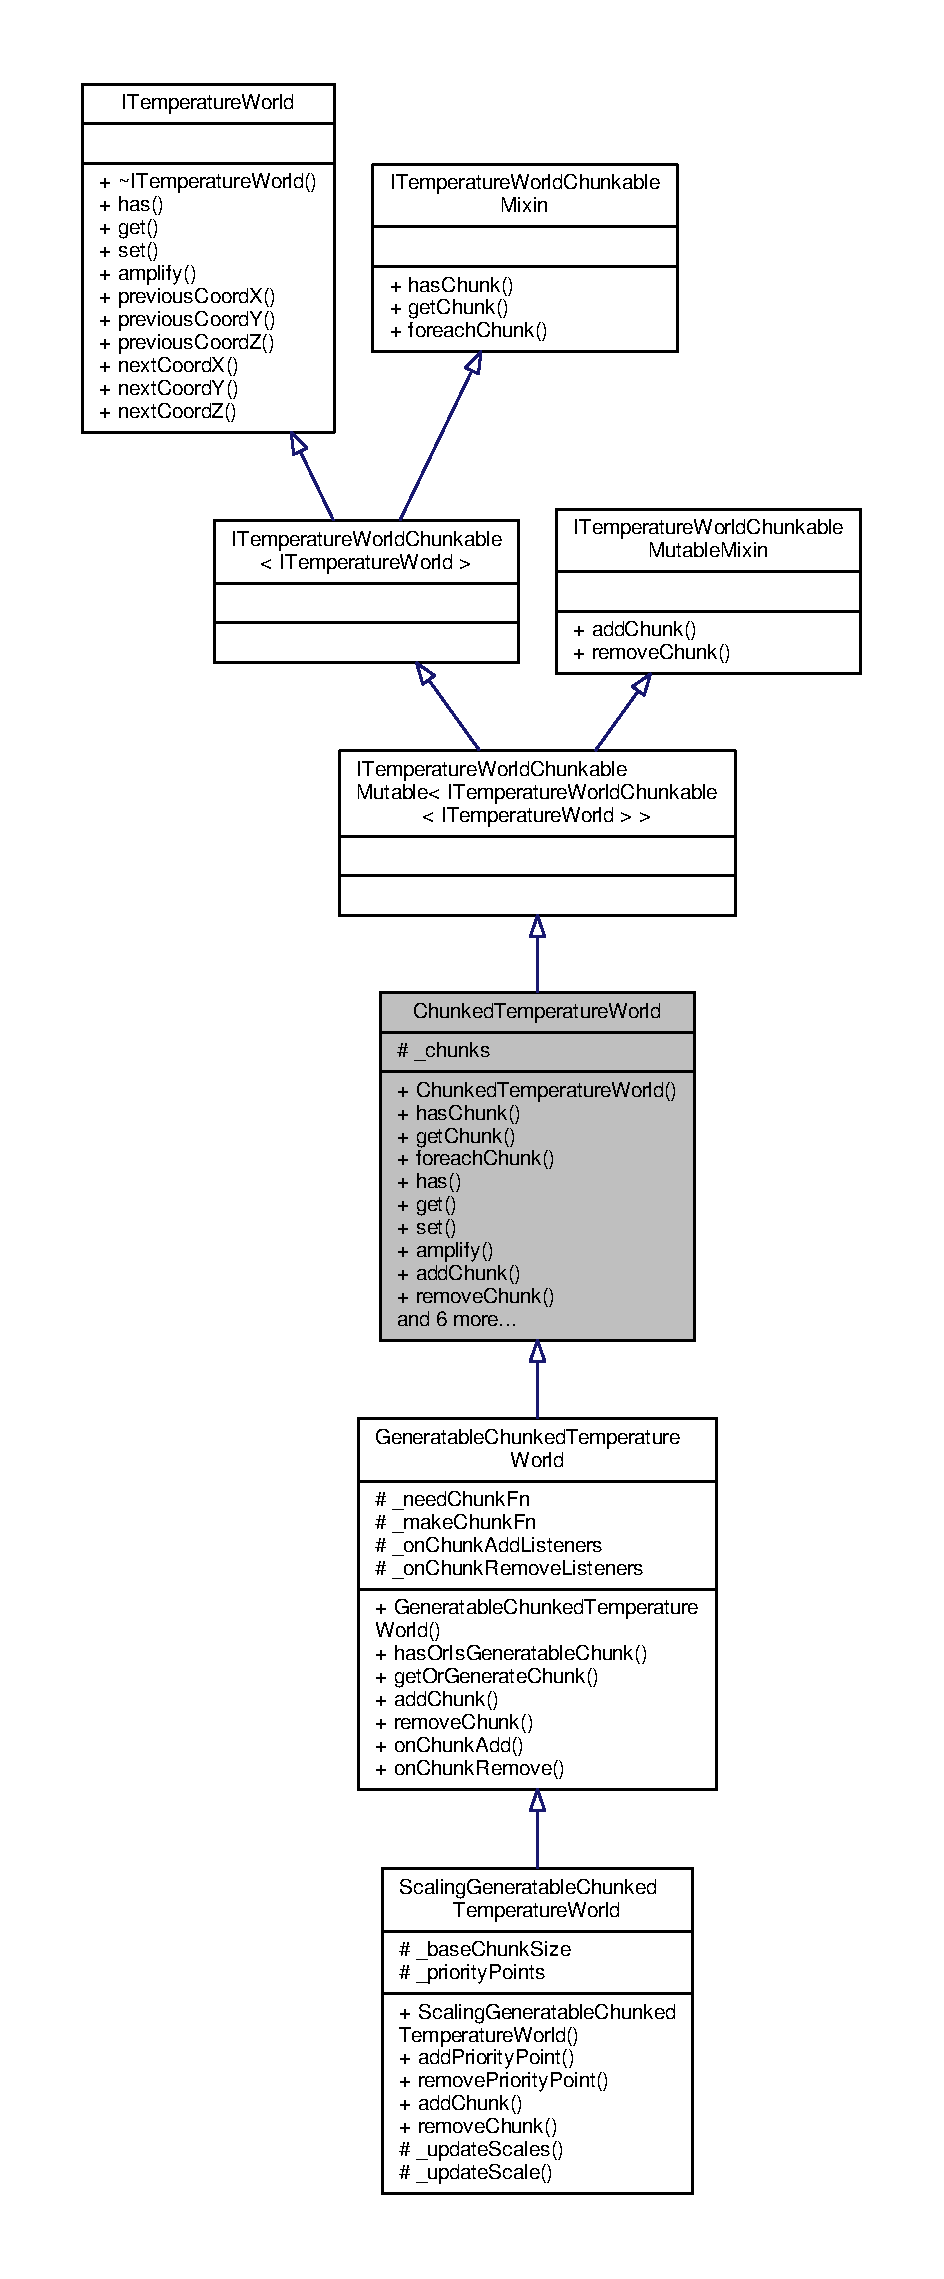
\includegraphics[height=550pt]{class_chunked_temperature_world__inherit__graph}
\end{center}
\end{figure}


Collaboration diagram for Chunked\-Temperature\-World\-:
\nopagebreak
\begin{figure}[H]
\begin{center}
\leavevmode
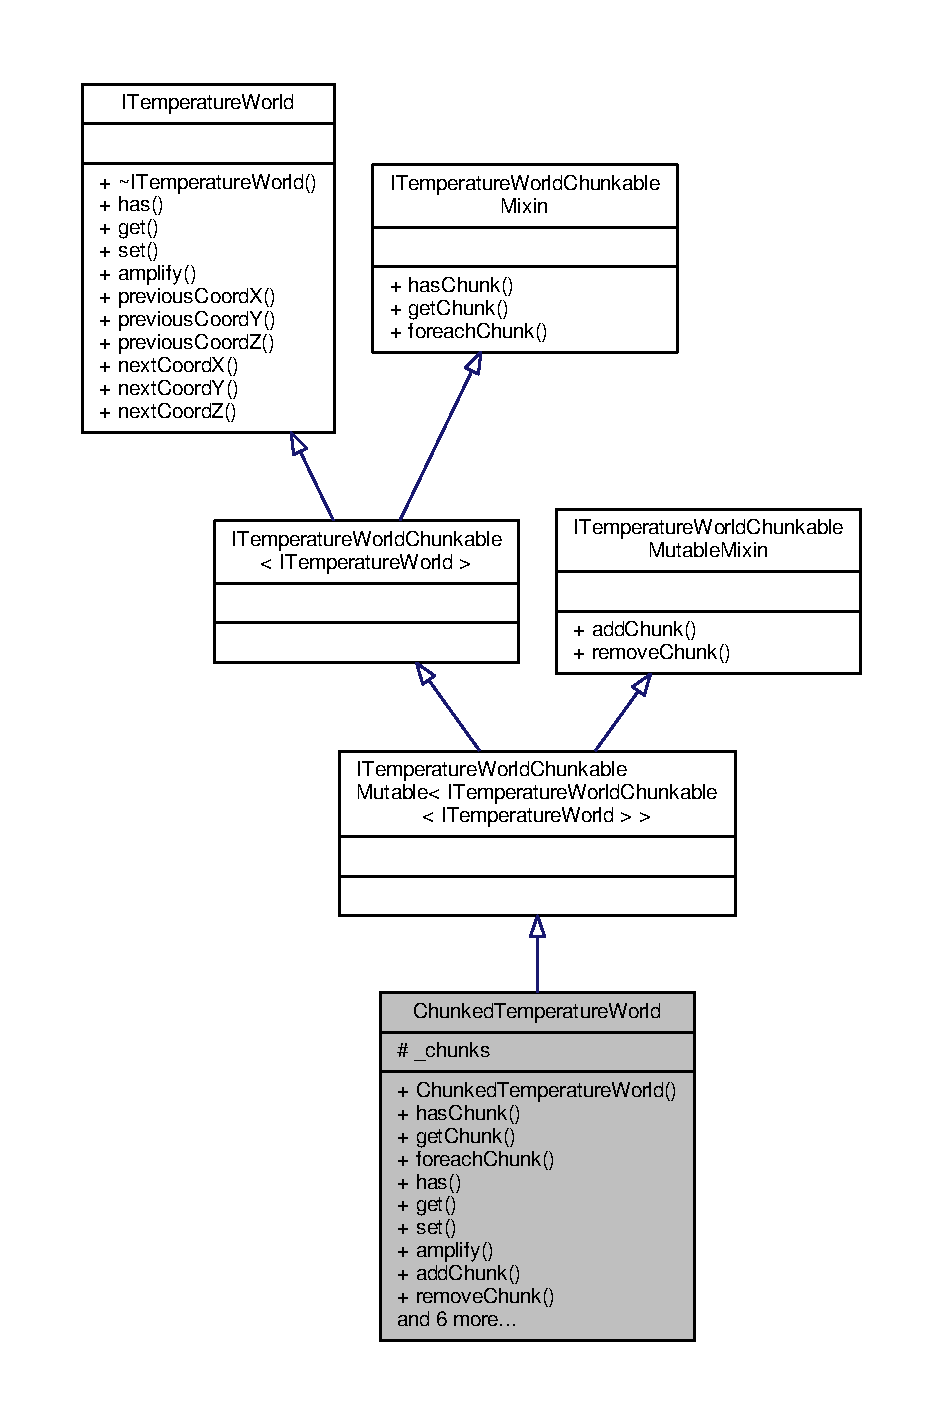
\includegraphics[width=350pt]{class_chunked_temperature_world__coll__graph}
\end{center}
\end{figure}
\subsection*{Public Member Functions}
\begin{DoxyCompactItemize}
\item 
\hyperlink{class_chunked_temperature_world_a9c60a8c8964e67556cc51a046f0cb42f}{Chunked\-Temperature\-World} ()
\item 
bool \hyperlink{class_chunked_temperature_world_aa06bb1517a6ba6537a89992a8a2f4d8e}{has\-Chunk} (\hyperlink{struct_coord}{Coord} x, \hyperlink{struct_coord}{Coord} y, \hyperlink{struct_coord}{Coord} z) const noexceptoverride
\item 
std\-::shared\-\_\-ptr\\*
$<$ \hyperlink{class_i_temperature_world_boundable}{I\-Temperature\-World\-Boundable}\\*
$<$ \hyperlink{class_i_temperature_world}{I\-Temperature\-World} $>$ $>$ \hyperlink{class_chunked_temperature_world_a9b925259d18aecbde683048ee0422d72}{get\-Chunk} (\hyperlink{struct_coord}{Coord} x, \hyperlink{struct_coord}{Coord} y, \hyperlink{struct_coord}{Coord} z) const override
\item 
void \hyperlink{class_chunked_temperature_world_ab737084e5879c35044c34012fd2281b3}{foreach\-Chunk} (\hyperlink{class_i_temperature_world_chunkable_mixin_abad666f407110d3370328bf97335c8be}{Foreach\-Chunk\-Fn} func) const override
\item 
bool \hyperlink{class_chunked_temperature_world_a05f4ce24ff44a6f4f17a8aac71f78af0}{has} (\hyperlink{struct_coord}{Coord} x, \hyperlink{struct_coord}{Coord} y, \hyperlink{struct_coord}{Coord} z) const noexceptoverride
\item 
\hyperlink{struct_temperature}{Temperature} \hyperlink{class_chunked_temperature_world_a9b57de410490bd8f5d6bc69d09d6b97c}{get} (\hyperlink{struct_coord}{Coord} x, \hyperlink{struct_coord}{Coord} y, \hyperlink{struct_coord}{Coord} z) const override
\item 
void \hyperlink{class_chunked_temperature_world_a97210f06e70f9ea07a4b284963e610e1}{set} (\hyperlink{struct_coord}{Coord} x, \hyperlink{struct_coord}{Coord} y, \hyperlink{struct_coord}{Coord} z, \hyperlink{struct_temperature}{Temperature} temperature) override
\item 
void \hyperlink{class_chunked_temperature_world_af4d90e4910f2197691f2c08f11cbc657}{amplify} (\hyperlink{struct_coord}{Coord} x, \hyperlink{struct_coord}{Coord} y, \hyperlink{struct_coord}{Coord} z, \hyperlink{struct_temperature}{Temperature} temperature) override
\item 
void \hyperlink{class_chunked_temperature_world_a5f9a3a143baf0c0238427926aef77f65}{add\-Chunk} (std\-::shared\-\_\-ptr$<$ \hyperlink{class_i_temperature_world_boundable}{I\-Temperature\-World\-Boundable}$<$ \hyperlink{class_i_temperature_world}{I\-Temperature\-World} $>$$>$ chunk) override
\item 
void \hyperlink{class_chunked_temperature_world_a623c1f5efe7aa84d428ba58365ee775a}{remove\-Chunk} (std\-::shared\-\_\-ptr$<$ \hyperlink{class_i_temperature_world_boundable}{I\-Temperature\-World\-Boundable}$<$ \hyperlink{class_i_temperature_world}{I\-Temperature\-World} $>$$>$ chunk) override
\item 
\hyperlink{struct_coord}{Coord} \hyperlink{class_chunked_temperature_world_a3e547d550f0558039561c18b8c74a329}{previous\-Coord\-X} (\hyperlink{struct_coord}{Coord} x) const noexceptoverride
\item 
\hyperlink{struct_coord}{Coord} \hyperlink{class_chunked_temperature_world_a510495c1304bed5444c53cbe8f30b31a}{previous\-Coord\-Y} (\hyperlink{struct_coord}{Coord} y) const noexceptoverride
\item 
\hyperlink{struct_coord}{Coord} \hyperlink{class_chunked_temperature_world_a0090b0b3cff4b12ffa543ff49ee6ba50}{previous\-Coord\-Z} (\hyperlink{struct_coord}{Coord} z) const noexceptoverride
\item 
\hyperlink{struct_coord}{Coord} \hyperlink{class_chunked_temperature_world_a42c80f4cc05ddf465e1ee08c2ed694f2}{next\-Coord\-X} (\hyperlink{struct_coord}{Coord} x) const noexceptoverride
\item 
\hyperlink{struct_coord}{Coord} \hyperlink{class_chunked_temperature_world_a5370203b68f8e248181a2a5647bfad7f}{next\-Coord\-Y} (\hyperlink{struct_coord}{Coord} y) const noexceptoverride
\item 
\hyperlink{struct_coord}{Coord} \hyperlink{class_chunked_temperature_world_ada9492462c81e605b92b3ac7c2f82f3e}{next\-Coord\-Z} (\hyperlink{struct_coord}{Coord} z) const noexceptoverride
\end{DoxyCompactItemize}
\subsection*{Protected Attributes}
\begin{DoxyCompactItemize}
\item 
std\-::list$<$ std\-::shared\-\_\-ptr\\*
$<$ \hyperlink{class_i_temperature_world_boundable}{I\-Temperature\-World\-Boundable}\\*
$<$ \hyperlink{class_i_temperature_world}{I\-Temperature\-World} $>$ $>$ $>$ \hyperlink{class_chunked_temperature_world_ac1ba488f612261643d130c060eb4611f}{\-\_\-chunks}
\end{DoxyCompactItemize}
\subsection*{Additional Inherited Members}


\subsection{Detailed Description}
Implementation of temperature world divided by chunks. It's backed by {\ttfamily std\-::list}. 

\subsection{Constructor \& Destructor Documentation}
\hypertarget{class_chunked_temperature_world_a9c60a8c8964e67556cc51a046f0cb42f}{\index{Chunked\-Temperature\-World@{Chunked\-Temperature\-World}!Chunked\-Temperature\-World@{Chunked\-Temperature\-World}}
\index{Chunked\-Temperature\-World@{Chunked\-Temperature\-World}!ChunkedTemperatureWorld@{Chunked\-Temperature\-World}}
\subsubsection[{Chunked\-Temperature\-World}]{\setlength{\rightskip}{0pt plus 5cm}Chunked\-Temperature\-World\-::\-Chunked\-Temperature\-World (
\begin{DoxyParamCaption}
{}
\end{DoxyParamCaption}
)}}\label{class_chunked_temperature_world_a9c60a8c8964e67556cc51a046f0cb42f}


\subsection{Member Function Documentation}
\hypertarget{class_chunked_temperature_world_a5f9a3a143baf0c0238427926aef77f65}{\index{Chunked\-Temperature\-World@{Chunked\-Temperature\-World}!add\-Chunk@{add\-Chunk}}
\index{add\-Chunk@{add\-Chunk}!ChunkedTemperatureWorld@{Chunked\-Temperature\-World}}
\subsubsection[{add\-Chunk}]{\setlength{\rightskip}{0pt plus 5cm}void Chunked\-Temperature\-World\-::add\-Chunk (
\begin{DoxyParamCaption}
\item[{std\-::shared\-\_\-ptr$<$ {\bf I\-Temperature\-World\-Boundable}$<$ {\bf I\-Temperature\-World} $>$$>$}]{chunk}
\end{DoxyParamCaption}
)\hspace{0.3cm}{\ttfamily [override]}, {\ttfamily [virtual]}}}\label{class_chunked_temperature_world_a5f9a3a143baf0c0238427926aef77f65}
Adds a chunk to this temperature world.


\begin{DoxyParams}{Parameters}
{\em chunk} & Chunk to add. \\
\hline
\end{DoxyParams}


Implements \hyperlink{class_i_temperature_world_chunkable_mutable_mixin_aad86bd1196ed595bcdd9025b9076085f}{I\-Temperature\-World\-Chunkable\-Mutable\-Mixin}.



Reimplemented in \hyperlink{class_scaling_generatable_chunked_temperature_world_a5ec1b1a2a5e058bf57bd7918fcc5a35b}{Scaling\-Generatable\-Chunked\-Temperature\-World}, and \hyperlink{class_generatable_chunked_temperature_world_af1a6752db0e722e8649ddb4c7e1ea8fa}{Generatable\-Chunked\-Temperature\-World}.



Here is the caller graph for this function\-:
\nopagebreak
\begin{figure}[H]
\begin{center}
\leavevmode
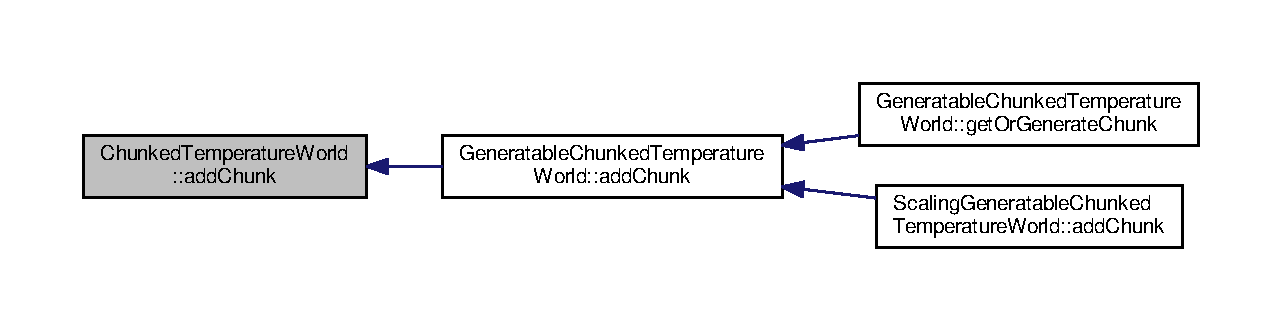
\includegraphics[width=350pt]{class_chunked_temperature_world_a5f9a3a143baf0c0238427926aef77f65_icgraph}
\end{center}
\end{figure}


\hypertarget{class_chunked_temperature_world_af4d90e4910f2197691f2c08f11cbc657}{\index{Chunked\-Temperature\-World@{Chunked\-Temperature\-World}!amplify@{amplify}}
\index{amplify@{amplify}!ChunkedTemperatureWorld@{Chunked\-Temperature\-World}}
\subsubsection[{amplify}]{\setlength{\rightskip}{0pt plus 5cm}void Chunked\-Temperature\-World\-::amplify (
\begin{DoxyParamCaption}
\item[{{\bf Coord}}]{x, }
\item[{{\bf Coord}}]{y, }
\item[{{\bf Coord}}]{z, }
\item[{{\bf Temperature}}]{temperature}
\end{DoxyParamCaption}
)\hspace{0.3cm}{\ttfamily [override]}, {\ttfamily [virtual]}}}\label{class_chunked_temperature_world_af4d90e4910f2197691f2c08f11cbc657}
Adds or substracts temperature value from existing temperature value at the point.


\begin{DoxyParams}{Parameters}
{\em x} & X coordinate. \\
\hline
{\em y} & Y coordinate. \\
\hline
{\em z} & Z coordinate. \\
\hline
{\em temperature} & \hyperlink{struct_temperature}{Temperature} difference. \\
\hline
\end{DoxyParams}


Implements \hyperlink{class_i_temperature_world_ac5a8a92e7141b2e2c2e3d66ba73b7c1e}{I\-Temperature\-World}.

\hypertarget{class_chunked_temperature_world_ab737084e5879c35044c34012fd2281b3}{\index{Chunked\-Temperature\-World@{Chunked\-Temperature\-World}!foreach\-Chunk@{foreach\-Chunk}}
\index{foreach\-Chunk@{foreach\-Chunk}!ChunkedTemperatureWorld@{Chunked\-Temperature\-World}}
\subsubsection[{foreach\-Chunk}]{\setlength{\rightskip}{0pt plus 5cm}void Chunked\-Temperature\-World\-::foreach\-Chunk (
\begin{DoxyParamCaption}
\item[{{\bf Foreach\-Chunk\-Fn}}]{func}
\end{DoxyParamCaption}
) const\hspace{0.3cm}{\ttfamily [override]}, {\ttfamily [virtual]}}}\label{class_chunked_temperature_world_ab737084e5879c35044c34012fd2281b3}
Loops over each chunk.


\begin{DoxyParams}{Parameters}
{\em func} & Function to execute at each chunk. \\
\hline
\end{DoxyParams}


Implements \hyperlink{class_i_temperature_world_chunkable_mixin_a2ded37900a83bdac968ff0f07f315225}{I\-Temperature\-World\-Chunkable\-Mixin}.

\hypertarget{class_chunked_temperature_world_a9b57de410490bd8f5d6bc69d09d6b97c}{\index{Chunked\-Temperature\-World@{Chunked\-Temperature\-World}!get@{get}}
\index{get@{get}!ChunkedTemperatureWorld@{Chunked\-Temperature\-World}}
\subsubsection[{get}]{\setlength{\rightskip}{0pt plus 5cm}{\bf Temperature} Chunked\-Temperature\-World\-::get (
\begin{DoxyParamCaption}
\item[{{\bf Coord}}]{x, }
\item[{{\bf Coord}}]{y, }
\item[{{\bf Coord}}]{z}
\end{DoxyParamCaption}
) const\hspace{0.3cm}{\ttfamily [override]}, {\ttfamily [virtual]}}}\label{class_chunked_temperature_world_a9b57de410490bd8f5d6bc69d09d6b97c}
Returns temperature at the point.


\begin{DoxyParams}{Parameters}
{\em x} & X coordinate. \\
\hline
{\em y} & Y coordinate. \\
\hline
{\em z} & Z coordinate. \\
\hline
\end{DoxyParams}
\begin{DoxyReturn}{Returns}
\hyperlink{struct_temperature}{Temperature} at the point. 
\end{DoxyReturn}


Implements \hyperlink{class_i_temperature_world_a9993df60754c2c89597bd8137568c12f}{I\-Temperature\-World}.

\hypertarget{class_chunked_temperature_world_a9b925259d18aecbde683048ee0422d72}{\index{Chunked\-Temperature\-World@{Chunked\-Temperature\-World}!get\-Chunk@{get\-Chunk}}
\index{get\-Chunk@{get\-Chunk}!ChunkedTemperatureWorld@{Chunked\-Temperature\-World}}
\subsubsection[{get\-Chunk}]{\setlength{\rightskip}{0pt plus 5cm}shared\-\_\-ptr$<$ {\bf I\-Temperature\-World\-Boundable}$<$ {\bf I\-Temperature\-World} $>$ $>$ Chunked\-Temperature\-World\-::get\-Chunk (
\begin{DoxyParamCaption}
\item[{{\bf Coord}}]{x, }
\item[{{\bf Coord}}]{y, }
\item[{{\bf Coord}}]{z}
\end{DoxyParamCaption}
) const\hspace{0.3cm}{\ttfamily [override]}, {\ttfamily [virtual]}}}\label{class_chunked_temperature_world_a9b925259d18aecbde683048ee0422d72}
Retrieves chunk which holds this point.


\begin{DoxyParams}{Parameters}
{\em x} & X coordinate. \\
\hline
{\em y} & Y coordinate. \\
\hline
{\em z} & Z coordinate. \\
\hline
\end{DoxyParams}
\begin{DoxyReturn}{Returns}
Chunk at the point. 
\end{DoxyReturn}


Implements \hyperlink{class_i_temperature_world_chunkable_mixin_aacb0fa709dbd3cb5d630dde64afec5b6}{I\-Temperature\-World\-Chunkable\-Mixin}.

\hypertarget{class_chunked_temperature_world_a05f4ce24ff44a6f4f17a8aac71f78af0}{\index{Chunked\-Temperature\-World@{Chunked\-Temperature\-World}!has@{has}}
\index{has@{has}!ChunkedTemperatureWorld@{Chunked\-Temperature\-World}}
\subsubsection[{has}]{\setlength{\rightskip}{0pt plus 5cm}bool Chunked\-Temperature\-World\-::has (
\begin{DoxyParamCaption}
\item[{{\bf Coord}}]{x, }
\item[{{\bf Coord}}]{y, }
\item[{{\bf Coord}}]{z}
\end{DoxyParamCaption}
) const\hspace{0.3cm}{\ttfamily [override]}, {\ttfamily [virtual]}, {\ttfamily [noexcept]}}}\label{class_chunked_temperature_world_a05f4ce24ff44a6f4f17a8aac71f78af0}
Tells whether temperature at the point is accessible. This method doesn't throw exceptions.


\begin{DoxyParams}{Parameters}
{\em x} & X coordinate. \\
\hline
{\em y} & Y coordinate. \\
\hline
{\em z} & Z coordinate. \\
\hline
\end{DoxyParams}
\begin{DoxyReturn}{Returns}
True if the point is accessible. 
\end{DoxyReturn}


Implements \hyperlink{class_i_temperature_world_a6c498247ed71d9ad037dd0c1b4779f81}{I\-Temperature\-World}.

\hypertarget{class_chunked_temperature_world_aa06bb1517a6ba6537a89992a8a2f4d8e}{\index{Chunked\-Temperature\-World@{Chunked\-Temperature\-World}!has\-Chunk@{has\-Chunk}}
\index{has\-Chunk@{has\-Chunk}!ChunkedTemperatureWorld@{Chunked\-Temperature\-World}}
\subsubsection[{has\-Chunk}]{\setlength{\rightskip}{0pt plus 5cm}bool Chunked\-Temperature\-World\-::has\-Chunk (
\begin{DoxyParamCaption}
\item[{{\bf Coord}}]{x, }
\item[{{\bf Coord}}]{y, }
\item[{{\bf Coord}}]{z}
\end{DoxyParamCaption}
) const\hspace{0.3cm}{\ttfamily [override]}, {\ttfamily [virtual]}, {\ttfamily [noexcept]}}}\label{class_chunked_temperature_world_aa06bb1517a6ba6537a89992a8a2f4d8e}
Tells whether the chunk which holds this point exists. This method doesn't throw exceptions.


\begin{DoxyParams}{Parameters}
{\em x} & X coordinate. \\
\hline
{\em y} & Y coordinate. \\
\hline
{\em z} & Z coordinate. \\
\hline
\end{DoxyParams}
\begin{DoxyReturn}{Returns}
True if chunk exists. 
\end{DoxyReturn}


Implements \hyperlink{class_i_temperature_world_chunkable_mixin_a4694b473f4e20976b8a538d16656943d}{I\-Temperature\-World\-Chunkable\-Mixin}.

\hypertarget{class_chunked_temperature_world_a42c80f4cc05ddf465e1ee08c2ed694f2}{\index{Chunked\-Temperature\-World@{Chunked\-Temperature\-World}!next\-Coord\-X@{next\-Coord\-X}}
\index{next\-Coord\-X@{next\-Coord\-X}!ChunkedTemperatureWorld@{Chunked\-Temperature\-World}}
\subsubsection[{next\-Coord\-X}]{\setlength{\rightskip}{0pt plus 5cm}{\bf Coord} Chunked\-Temperature\-World\-::next\-Coord\-X (
\begin{DoxyParamCaption}
\item[{{\bf Coord}}]{x}
\end{DoxyParamCaption}
) const\hspace{0.3cm}{\ttfamily [override]}, {\ttfamily [virtual]}, {\ttfamily [noexcept]}}}\label{class_chunked_temperature_world_a42c80f4cc05ddf465e1ee08c2ed694f2}

\begin{DoxyParams}{Parameters}
{\em x} & Current coordinate by x axis. \\
\hline
\end{DoxyParams}
\begin{DoxyReturn}{Returns}
Next coordinate by x axis. 
\end{DoxyReturn}


Implements \hyperlink{class_i_temperature_world_ae1daa3e639084e2c25d78ba1c9841353}{I\-Temperature\-World}.

\hypertarget{class_chunked_temperature_world_a5370203b68f8e248181a2a5647bfad7f}{\index{Chunked\-Temperature\-World@{Chunked\-Temperature\-World}!next\-Coord\-Y@{next\-Coord\-Y}}
\index{next\-Coord\-Y@{next\-Coord\-Y}!ChunkedTemperatureWorld@{Chunked\-Temperature\-World}}
\subsubsection[{next\-Coord\-Y}]{\setlength{\rightskip}{0pt plus 5cm}{\bf Coord} Chunked\-Temperature\-World\-::next\-Coord\-Y (
\begin{DoxyParamCaption}
\item[{{\bf Coord}}]{y}
\end{DoxyParamCaption}
) const\hspace{0.3cm}{\ttfamily [override]}, {\ttfamily [virtual]}, {\ttfamily [noexcept]}}}\label{class_chunked_temperature_world_a5370203b68f8e248181a2a5647bfad7f}

\begin{DoxyParams}{Parameters}
{\em y} & Current coordinate by y axis. \\
\hline
\end{DoxyParams}
\begin{DoxyReturn}{Returns}
Next coordinate by y axis. 
\end{DoxyReturn}


Implements \hyperlink{class_i_temperature_world_a4c56188c251aee5dc5edea440ad288b5}{I\-Temperature\-World}.

\hypertarget{class_chunked_temperature_world_ada9492462c81e605b92b3ac7c2f82f3e}{\index{Chunked\-Temperature\-World@{Chunked\-Temperature\-World}!next\-Coord\-Z@{next\-Coord\-Z}}
\index{next\-Coord\-Z@{next\-Coord\-Z}!ChunkedTemperatureWorld@{Chunked\-Temperature\-World}}
\subsubsection[{next\-Coord\-Z}]{\setlength{\rightskip}{0pt plus 5cm}{\bf Coord} Chunked\-Temperature\-World\-::next\-Coord\-Z (
\begin{DoxyParamCaption}
\item[{{\bf Coord}}]{z}
\end{DoxyParamCaption}
) const\hspace{0.3cm}{\ttfamily [override]}, {\ttfamily [virtual]}, {\ttfamily [noexcept]}}}\label{class_chunked_temperature_world_ada9492462c81e605b92b3ac7c2f82f3e}

\begin{DoxyParams}{Parameters}
{\em z} & Current coordinate by z axis. \\
\hline
\end{DoxyParams}
\begin{DoxyReturn}{Returns}
Next coordinate by z axis. 
\end{DoxyReturn}


Implements \hyperlink{class_i_temperature_world_aeea34ba0bf416143309a0cf046ad1dce}{I\-Temperature\-World}.

\hypertarget{class_chunked_temperature_world_a3e547d550f0558039561c18b8c74a329}{\index{Chunked\-Temperature\-World@{Chunked\-Temperature\-World}!previous\-Coord\-X@{previous\-Coord\-X}}
\index{previous\-Coord\-X@{previous\-Coord\-X}!ChunkedTemperatureWorld@{Chunked\-Temperature\-World}}
\subsubsection[{previous\-Coord\-X}]{\setlength{\rightskip}{0pt plus 5cm}{\bf Coord} Chunked\-Temperature\-World\-::previous\-Coord\-X (
\begin{DoxyParamCaption}
\item[{{\bf Coord}}]{x}
\end{DoxyParamCaption}
) const\hspace{0.3cm}{\ttfamily [override]}, {\ttfamily [virtual]}, {\ttfamily [noexcept]}}}\label{class_chunked_temperature_world_a3e547d550f0558039561c18b8c74a329}

\begin{DoxyParams}{Parameters}
{\em x} & Current coordinate by x axis. \\
\hline
\end{DoxyParams}
\begin{DoxyReturn}{Returns}
Previous coordinate by x axis. 
\end{DoxyReturn}


Implements \hyperlink{class_i_temperature_world_adfa6f4c698d6407000314d9d43fe6c5d}{I\-Temperature\-World}.

\hypertarget{class_chunked_temperature_world_a510495c1304bed5444c53cbe8f30b31a}{\index{Chunked\-Temperature\-World@{Chunked\-Temperature\-World}!previous\-Coord\-Y@{previous\-Coord\-Y}}
\index{previous\-Coord\-Y@{previous\-Coord\-Y}!ChunkedTemperatureWorld@{Chunked\-Temperature\-World}}
\subsubsection[{previous\-Coord\-Y}]{\setlength{\rightskip}{0pt plus 5cm}{\bf Coord} Chunked\-Temperature\-World\-::previous\-Coord\-Y (
\begin{DoxyParamCaption}
\item[{{\bf Coord}}]{y}
\end{DoxyParamCaption}
) const\hspace{0.3cm}{\ttfamily [override]}, {\ttfamily [virtual]}, {\ttfamily [noexcept]}}}\label{class_chunked_temperature_world_a510495c1304bed5444c53cbe8f30b31a}

\begin{DoxyParams}{Parameters}
{\em y} & Current coordinate by y axis. \\
\hline
\end{DoxyParams}
\begin{DoxyReturn}{Returns}
Previous coordinate by y axis. 
\end{DoxyReturn}


Implements \hyperlink{class_i_temperature_world_ab74e8cf0b0261ee342e356c1212ff9a2}{I\-Temperature\-World}.

\hypertarget{class_chunked_temperature_world_a0090b0b3cff4b12ffa543ff49ee6ba50}{\index{Chunked\-Temperature\-World@{Chunked\-Temperature\-World}!previous\-Coord\-Z@{previous\-Coord\-Z}}
\index{previous\-Coord\-Z@{previous\-Coord\-Z}!ChunkedTemperatureWorld@{Chunked\-Temperature\-World}}
\subsubsection[{previous\-Coord\-Z}]{\setlength{\rightskip}{0pt plus 5cm}{\bf Coord} Chunked\-Temperature\-World\-::previous\-Coord\-Z (
\begin{DoxyParamCaption}
\item[{{\bf Coord}}]{z}
\end{DoxyParamCaption}
) const\hspace{0.3cm}{\ttfamily [override]}, {\ttfamily [virtual]}, {\ttfamily [noexcept]}}}\label{class_chunked_temperature_world_a0090b0b3cff4b12ffa543ff49ee6ba50}

\begin{DoxyParams}{Parameters}
{\em z} & Current coordinate by z axis. \\
\hline
\end{DoxyParams}
\begin{DoxyReturn}{Returns}
Previous coordinate by z axis. 
\end{DoxyReturn}


Implements \hyperlink{class_i_temperature_world_a7ed125d1e71c39dc06cbe64ba58662c5}{I\-Temperature\-World}.

\hypertarget{class_chunked_temperature_world_a623c1f5efe7aa84d428ba58365ee775a}{\index{Chunked\-Temperature\-World@{Chunked\-Temperature\-World}!remove\-Chunk@{remove\-Chunk}}
\index{remove\-Chunk@{remove\-Chunk}!ChunkedTemperatureWorld@{Chunked\-Temperature\-World}}
\subsubsection[{remove\-Chunk}]{\setlength{\rightskip}{0pt plus 5cm}void Chunked\-Temperature\-World\-::remove\-Chunk (
\begin{DoxyParamCaption}
\item[{std\-::shared\-\_\-ptr$<$ {\bf I\-Temperature\-World\-Boundable}$<$ {\bf I\-Temperature\-World} $>$$>$}]{chunk}
\end{DoxyParamCaption}
)\hspace{0.3cm}{\ttfamily [override]}, {\ttfamily [virtual]}}}\label{class_chunked_temperature_world_a623c1f5efe7aa84d428ba58365ee775a}
Removes chunk from this temperature world.


\begin{DoxyParams}{Parameters}
{\em chunk} & Chunk to remove. \\
\hline
\end{DoxyParams}


Implements \hyperlink{class_i_temperature_world_chunkable_mutable_mixin_a52a6ebbd24162b00566f8e5b535878f8}{I\-Temperature\-World\-Chunkable\-Mutable\-Mixin}.



Reimplemented in \hyperlink{class_scaling_generatable_chunked_temperature_world_ac3ae4d696d934b925076eeab88658978}{Scaling\-Generatable\-Chunked\-Temperature\-World}, and \hyperlink{class_generatable_chunked_temperature_world_a42c646343bb79dcdeb9f96e6aa06cbec}{Generatable\-Chunked\-Temperature\-World}.



Here is the caller graph for this function\-:
\nopagebreak
\begin{figure}[H]
\begin{center}
\leavevmode
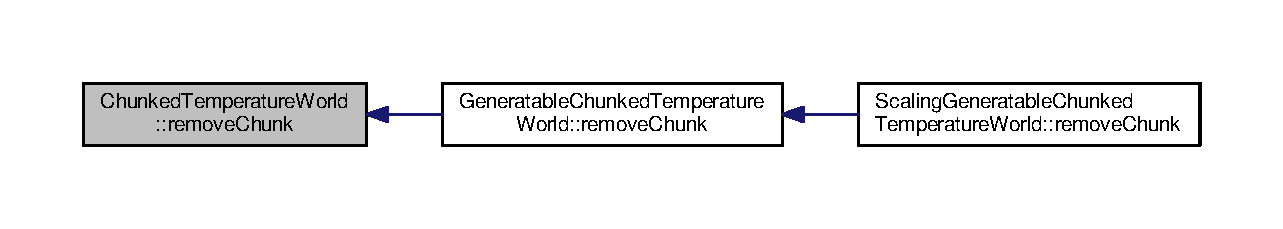
\includegraphics[width=350pt]{class_chunked_temperature_world_a623c1f5efe7aa84d428ba58365ee775a_icgraph}
\end{center}
\end{figure}


\hypertarget{class_chunked_temperature_world_a97210f06e70f9ea07a4b284963e610e1}{\index{Chunked\-Temperature\-World@{Chunked\-Temperature\-World}!set@{set}}
\index{set@{set}!ChunkedTemperatureWorld@{Chunked\-Temperature\-World}}
\subsubsection[{set}]{\setlength{\rightskip}{0pt plus 5cm}void Chunked\-Temperature\-World\-::set (
\begin{DoxyParamCaption}
\item[{{\bf Coord}}]{x, }
\item[{{\bf Coord}}]{y, }
\item[{{\bf Coord}}]{z, }
\item[{{\bf Temperature}}]{temperature}
\end{DoxyParamCaption}
)\hspace{0.3cm}{\ttfamily [override]}, {\ttfamily [virtual]}}}\label{class_chunked_temperature_world_a97210f06e70f9ea07a4b284963e610e1}
Sets temperature at the point.


\begin{DoxyParams}{Parameters}
{\em x} & X coordinate. \\
\hline
{\em y} & Y coordinate. \\
\hline
{\em z} & Z coordinate. \\
\hline
{\em temperature} & \hyperlink{struct_temperature}{Temperature} to set. \\
\hline
\end{DoxyParams}


Implements \hyperlink{class_i_temperature_world_ab23db7ec9a890d6dbb172b26c2fd3d00}{I\-Temperature\-World}.



\subsection{Member Data Documentation}
\hypertarget{class_chunked_temperature_world_ac1ba488f612261643d130c060eb4611f}{\index{Chunked\-Temperature\-World@{Chunked\-Temperature\-World}!\-\_\-chunks@{\-\_\-chunks}}
\index{\-\_\-chunks@{\-\_\-chunks}!ChunkedTemperatureWorld@{Chunked\-Temperature\-World}}
\subsubsection[{\-\_\-chunks}]{\setlength{\rightskip}{0pt plus 5cm}std\-::list$<$std\-::shared\-\_\-ptr$<${\bf I\-Temperature\-World\-Boundable}$<${\bf I\-Temperature\-World}$>$ $>$ $>$ Chunked\-Temperature\-World\-::\-\_\-chunks\hspace{0.3cm}{\ttfamily [protected]}}}\label{class_chunked_temperature_world_ac1ba488f612261643d130c060eb4611f}


The documentation for this class was generated from the following files\-:\begin{DoxyCompactItemize}
\item 
/home/travis/build/glitchless/\-Recast/src/headers/temperature-\/world/implementation/\hyperlink{_chunked_temperature_world_8hpp}{Chunked\-Temperature\-World.\-hpp}\item 
/home/travis/build/glitchless/\-Recast/src/temperature-\/world/implementation/\hyperlink{_chunked_temperature_world_8cpp}{Chunked\-Temperature\-World.\-cpp}\end{DoxyCompactItemize}

\hypertarget{class_command_manager}{\section{Command\-Manager Class Reference}
\label{class_command_manager}\index{Command\-Manager@{Command\-Manager}}
}


Send string-\/command through \hyperlink{class_command_manager}{Command\-Manager}.  




{\ttfamily \#include $<$Command\-Manager.\-hpp$>$}



Collaboration diagram for Command\-Manager\-:
\nopagebreak
\begin{figure}[H]
\begin{center}
\leavevmode
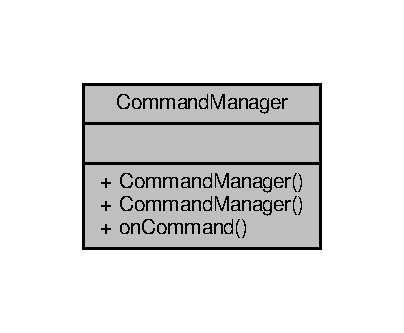
\includegraphics[width=246pt]{class_command_manager__coll__graph}
\end{center}
\end{figure}
\subsection*{Public Member Functions}
\begin{DoxyCompactItemize}
\item 
\hyperlink{class_command_manager_a8a13226bf933396a3f35dfb5bee3e813}{Command\-Manager} ()
\begin{DoxyCompactList}\small\item\em Init \hyperlink{class_command_manager}{Command\-Manager}. \end{DoxyCompactList}\item 
\hyperlink{class_command_manager_aeaffe7fa7dd8f1dd45b642120013a076}{Command\-Manager} (const \hyperlink{class_command_manager}{Command\-Manager} \&other)=delete
\item 
void \hyperlink{class_command_manager_abef8721bbe32e1ecb22f2f3d3b8c0601}{on\-Command} (\hyperlink{class_i_command_sender}{I\-Command\-Sender} $\ast$sender, const std\-::string \&cmd)
\item 
void \hyperlink{class_command_manager_a6782f9787d0e35ee3cc0eff69f764fa2}{execute\-Delayed\-Command\-In\-U\-I} ()
\end{DoxyCompactItemize}


\subsection{Detailed Description}
Send string-\/command through \hyperlink{class_command_manager}{Command\-Manager}. 

This is a very important class. Through this you can execute console-\/like text commands. 

\subsection{Constructor \& Destructor Documentation}
\hypertarget{class_command_manager_a8a13226bf933396a3f35dfb5bee3e813}{\index{Command\-Manager@{Command\-Manager}!Command\-Manager@{Command\-Manager}}
\index{Command\-Manager@{Command\-Manager}!CommandManager@{Command\-Manager}}
\subsubsection[{Command\-Manager}]{\setlength{\rightskip}{0pt plus 5cm}Command\-Manager\-::\-Command\-Manager (
\begin{DoxyParamCaption}
{}
\end{DoxyParamCaption}
)}}\label{class_command_manager_a8a13226bf933396a3f35dfb5bee3e813}


Init \hyperlink{class_command_manager}{Command\-Manager}. 

Adding all objects that extend \hyperlink{class_i_command}{I\-Command} to list (std\-::vector).

\begin{DoxyWarning}{Warning}
If you add an \hyperlink{class_i_command}{I\-Command}, you should add line here 
\end{DoxyWarning}
\hypertarget{class_command_manager_aeaffe7fa7dd8f1dd45b642120013a076}{\index{Command\-Manager@{Command\-Manager}!Command\-Manager@{Command\-Manager}}
\index{Command\-Manager@{Command\-Manager}!CommandManager@{Command\-Manager}}
\subsubsection[{Command\-Manager}]{\setlength{\rightskip}{0pt plus 5cm}Command\-Manager\-::\-Command\-Manager (
\begin{DoxyParamCaption}
\item[{const {\bf Command\-Manager} \&}]{other}
\end{DoxyParamCaption}
)\hspace{0.3cm}{\ttfamily [delete]}}}\label{class_command_manager_aeaffe7fa7dd8f1dd45b642120013a076}


\subsection{Member Function Documentation}
\hypertarget{class_command_manager_a6782f9787d0e35ee3cc0eff69f764fa2}{\index{Command\-Manager@{Command\-Manager}!execute\-Delayed\-Command\-In\-U\-I@{execute\-Delayed\-Command\-In\-U\-I}}
\index{execute\-Delayed\-Command\-In\-U\-I@{execute\-Delayed\-Command\-In\-U\-I}!CommandManager@{Command\-Manager}}
\subsubsection[{execute\-Delayed\-Command\-In\-U\-I}]{\setlength{\rightskip}{0pt plus 5cm}void Command\-Manager\-::execute\-Delayed\-Command\-In\-U\-I (
\begin{DoxyParamCaption}
{}
\end{DoxyParamCaption}
)}}\label{class_command_manager_a6782f9787d0e35ee3cc0eff69f764fa2}


Here is the call graph for this function\-:
\nopagebreak
\begin{figure}[H]
\begin{center}
\leavevmode
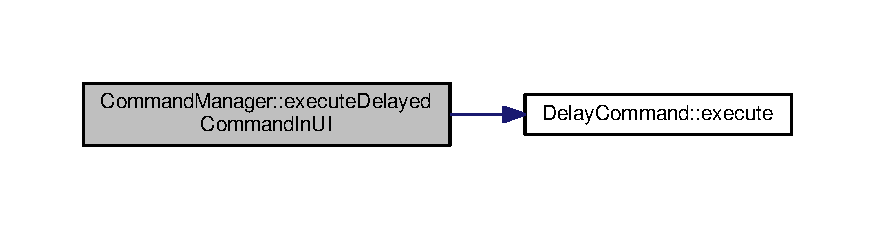
\includegraphics[width=350pt]{class_command_manager_a6782f9787d0e35ee3cc0eff69f764fa2_cgraph}
\end{center}
\end{figure}


\hypertarget{class_command_manager_abef8721bbe32e1ecb22f2f3d3b8c0601}{\index{Command\-Manager@{Command\-Manager}!on\-Command@{on\-Command}}
\index{on\-Command@{on\-Command}!CommandManager@{Command\-Manager}}
\subsubsection[{on\-Command}]{\setlength{\rightskip}{0pt plus 5cm}void Command\-Manager\-::on\-Command (
\begin{DoxyParamCaption}
\item[{{\bf I\-Command\-Sender} $\ast$}]{sender, }
\item[{const std\-::string \&}]{cmd}
\end{DoxyParamCaption}
)}}\label{class_command_manager_abef8721bbe32e1ecb22f2f3d3b8c0601}


Here is the call graph for this function\-:
\nopagebreak
\begin{figure}[H]
\begin{center}
\leavevmode
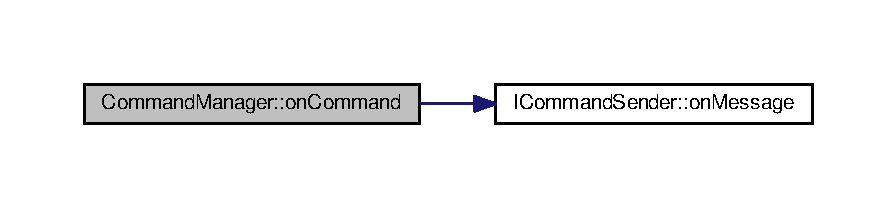
\includegraphics[width=350pt]{class_command_manager_abef8721bbe32e1ecb22f2f3d3b8c0601_cgraph}
\end{center}
\end{figure}




The documentation for this class was generated from the following files\-:\begin{DoxyCompactItemize}
\item 
/home/travis/build/bender-\/wardrobe/\-Recast/src/headers/commands/\hyperlink{_command_manager_8hpp}{Command\-Manager.\-hpp}\item 
/home/travis/build/bender-\/wardrobe/\-Recast/src/core/commands/\hyperlink{_command_manager_8cpp}{Command\-Manager.\-cpp}\end{DoxyCompactItemize}

\hypertarget{class_config}{\section{Config Class Reference}
\label{class_config}\index{Config@{Config}}
}


\hyperlink{class_config}{Config} class.  




{\ttfamily \#include $<$Config.\-hpp$>$}



Collaboration diagram for Config\-:
\nopagebreak
\begin{figure}[H]
\begin{center}
\leavevmode
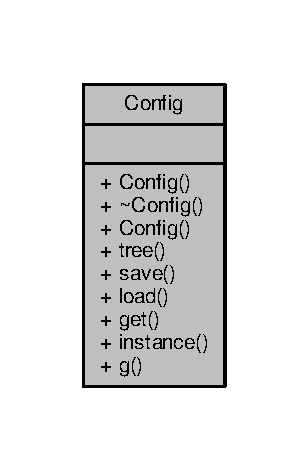
\includegraphics[width=148pt]{class_config__coll__graph}
\end{center}
\end{figure}
\subsection*{Public Member Functions}
\begin{DoxyCompactItemize}
\item 
\hyperlink{class_config_abc51a2c710c8666d27b53cc03597201d}{Config} (const std\-::string \&filename)
\item 
\hyperlink{class_config_a543dce59b66475c5108088ee4ce1cdfc}{$\sim$\-Config} ()
\item 
\hyperlink{class_config_aea1b7e862074892ee39a5583c342c482}{Config} (const \hyperlink{class_config}{Config} \&other)=delete
\item 
boost\-::property\-\_\-tree\-::ptree \& \hyperlink{class_config_a006701bd126aa5809b3a15e75c63bfb6}{tree} ()
\item 
void \hyperlink{class_config_ae7e68962f22a2c965a61702de1c637db}{save} ()
\item 
void \hyperlink{class_config_add4ebd0c89505c9b5368f03264555606}{load} ()
\item 
{\footnotesize template$<$class T $>$ }\\T \hyperlink{class_config_a1f8e429f853f20cac7cf128f2b71543e}{get} (const std\-::string \&key, T default\-Var)
\end{DoxyCompactItemize}
\subsection*{Static Public Member Functions}
\begin{DoxyCompactItemize}
\item 
static \hyperlink{class_config}{Config} $\ast$ \hyperlink{class_config_abf1d4539011ef83cac0fef2ac864a3a9}{instance} ()
\item 
{\footnotesize template$<$class T $>$ }\\static T \hyperlink{class_config_aaff6aaabead6b7486ec122f9dda807fd}{g} (const std\-::string \&key, T default\-Var)
\end{DoxyCompactItemize}


\subsection{Detailed Description}
\hyperlink{class_config}{Config} class. 

Using Boost ptree struct. \hyperlink{class_config}{Config} file hashing and buffering in memory. (You can't get an instance of \hyperlink{class_config}{Config} from constructor) Please call \hyperlink{class_config_abf1d4539011ef83cac0fef2ac864a3a9}{Config\-::instance} to get an instance of \hyperlink{class_config}{Config}. 

\subsection{Constructor \& Destructor Documentation}
\hypertarget{class_config_abc51a2c710c8666d27b53cc03597201d}{\index{Config@{Config}!Config@{Config}}
\index{Config@{Config}!Config@{Config}}
\subsubsection[{Config}]{\setlength{\rightskip}{0pt plus 5cm}Config\-::\-Config (
\begin{DoxyParamCaption}
\item[{const std\-::string \&}]{filename}
\end{DoxyParamCaption}
)}}\label{class_config_abc51a2c710c8666d27b53cc03597201d}
\hypertarget{class_config_a543dce59b66475c5108088ee4ce1cdfc}{\index{Config@{Config}!$\sim$\-Config@{$\sim$\-Config}}
\index{$\sim$\-Config@{$\sim$\-Config}!Config@{Config}}
\subsubsection[{$\sim$\-Config}]{\setlength{\rightskip}{0pt plus 5cm}Config\-::$\sim$\-Config (
\begin{DoxyParamCaption}
{}
\end{DoxyParamCaption}
)}}\label{class_config_a543dce59b66475c5108088ee4ce1cdfc}
\hypertarget{class_config_aea1b7e862074892ee39a5583c342c482}{\index{Config@{Config}!Config@{Config}}
\index{Config@{Config}!Config@{Config}}
\subsubsection[{Config}]{\setlength{\rightskip}{0pt plus 5cm}Config\-::\-Config (
\begin{DoxyParamCaption}
\item[{const {\bf Config} \&}]{other}
\end{DoxyParamCaption}
)\hspace{0.3cm}{\ttfamily [delete]}}}\label{class_config_aea1b7e862074892ee39a5583c342c482}


\subsection{Member Function Documentation}
\hypertarget{class_config_aaff6aaabead6b7486ec122f9dda807fd}{\index{Config@{Config}!g@{g}}
\index{g@{g}!Config@{Config}}
\subsubsection[{g}]{\setlength{\rightskip}{0pt plus 5cm}template$<$class T $>$ static T Config\-::g (
\begin{DoxyParamCaption}
\item[{const std\-::string \&}]{key, }
\item[{T}]{default\-Var}
\end{DoxyParamCaption}
)\hspace{0.3cm}{\ttfamily [inline]}, {\ttfamily [static]}}}\label{class_config_aaff6aaabead6b7486ec122f9dda807fd}


Here is the call graph for this function\-:
\nopagebreak
\begin{figure}[H]
\begin{center}
\leavevmode
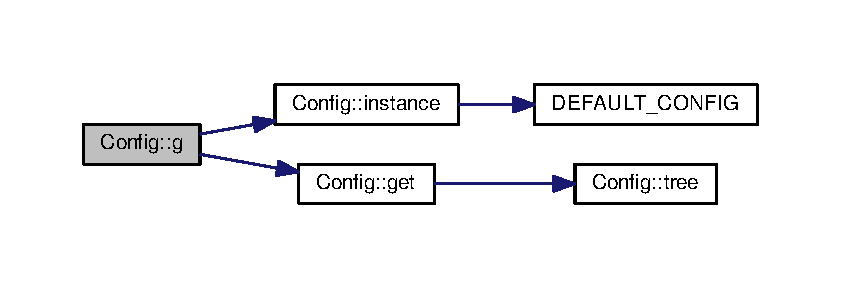
\includegraphics[width=350pt]{class_config_aaff6aaabead6b7486ec122f9dda807fd_cgraph}
\end{center}
\end{figure}




Here is the caller graph for this function\-:
\nopagebreak
\begin{figure}[H]
\begin{center}
\leavevmode
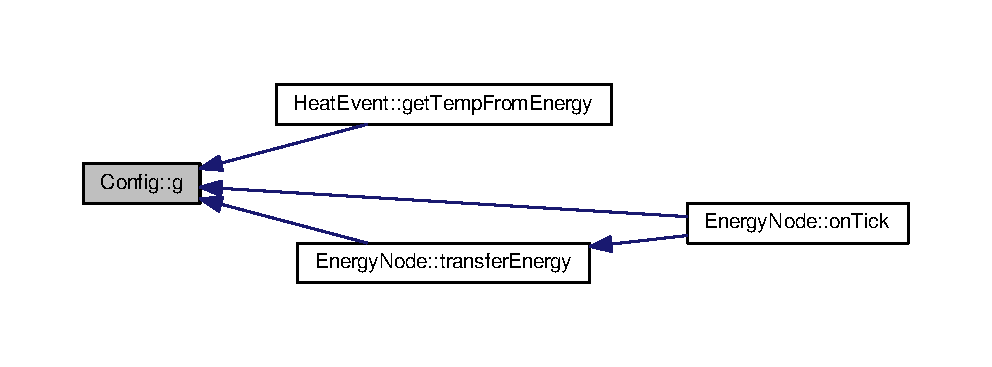
\includegraphics[width=350pt]{class_config_aaff6aaabead6b7486ec122f9dda807fd_icgraph}
\end{center}
\end{figure}


\hypertarget{class_config_a1f8e429f853f20cac7cf128f2b71543e}{\index{Config@{Config}!get@{get}}
\index{get@{get}!Config@{Config}}
\subsubsection[{get}]{\setlength{\rightskip}{0pt plus 5cm}template$<$class T $>$ T Config\-::get (
\begin{DoxyParamCaption}
\item[{const std\-::string \&}]{key, }
\item[{T}]{default\-Var}
\end{DoxyParamCaption}
)\hspace{0.3cm}{\ttfamily [inline]}}}\label{class_config_a1f8e429f853f20cac7cf128f2b71543e}
This method create param if not exist


\begin{DoxyTemplParams}{Template Parameters}
{\em T} & class of config var \\
\hline
\end{DoxyTemplParams}

\begin{DoxyParams}{Parameters}
{\em key} & string with path like 'general.\-server.\-port' \\
\hline
{\em default\-Var} & var used when config var is empty \\
\hline
\end{DoxyParams}
\begin{DoxyReturn}{Returns}
defult\-Var returned if config var is empty 
\end{DoxyReturn}


Here is the call graph for this function\-:
\nopagebreak
\begin{figure}[H]
\begin{center}
\leavevmode
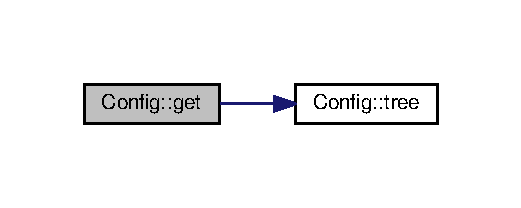
\includegraphics[width=250pt]{class_config_a1f8e429f853f20cac7cf128f2b71543e_cgraph}
\end{center}
\end{figure}




Here is the caller graph for this function\-:
\nopagebreak
\begin{figure}[H]
\begin{center}
\leavevmode
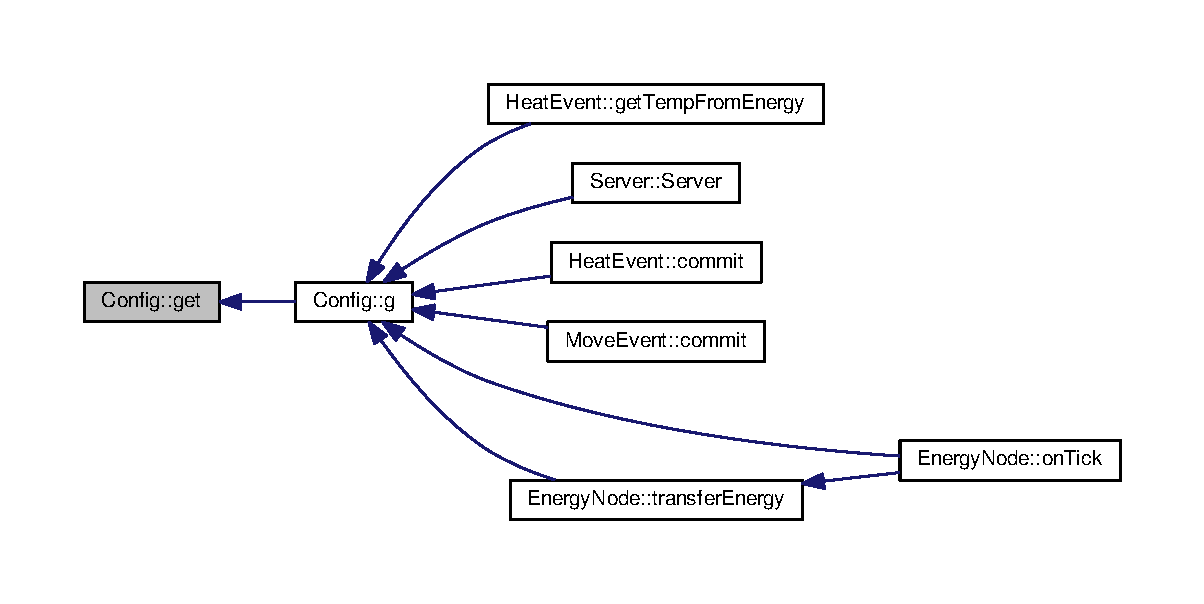
\includegraphics[width=350pt]{class_config_a1f8e429f853f20cac7cf128f2b71543e_icgraph}
\end{center}
\end{figure}


\hypertarget{class_config_abf1d4539011ef83cac0fef2ac864a3a9}{\index{Config@{Config}!instance@{instance}}
\index{instance@{instance}!Config@{Config}}
\subsubsection[{instance}]{\setlength{\rightskip}{0pt plus 5cm}{\bf Config} $\ast$ Config\-::instance (
\begin{DoxyParamCaption}
{}
\end{DoxyParamCaption}
)\hspace{0.3cm}{\ttfamily [static]}}}\label{class_config_abf1d4539011ef83cac0fef2ac864a3a9}


Here is the call graph for this function\-:
\nopagebreak
\begin{figure}[H]
\begin{center}
\leavevmode
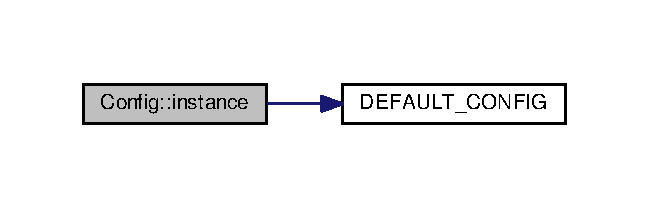
\includegraphics[width=312pt]{class_config_abf1d4539011ef83cac0fef2ac864a3a9_cgraph}
\end{center}
\end{figure}




Here is the caller graph for this function\-:
\nopagebreak
\begin{figure}[H]
\begin{center}
\leavevmode
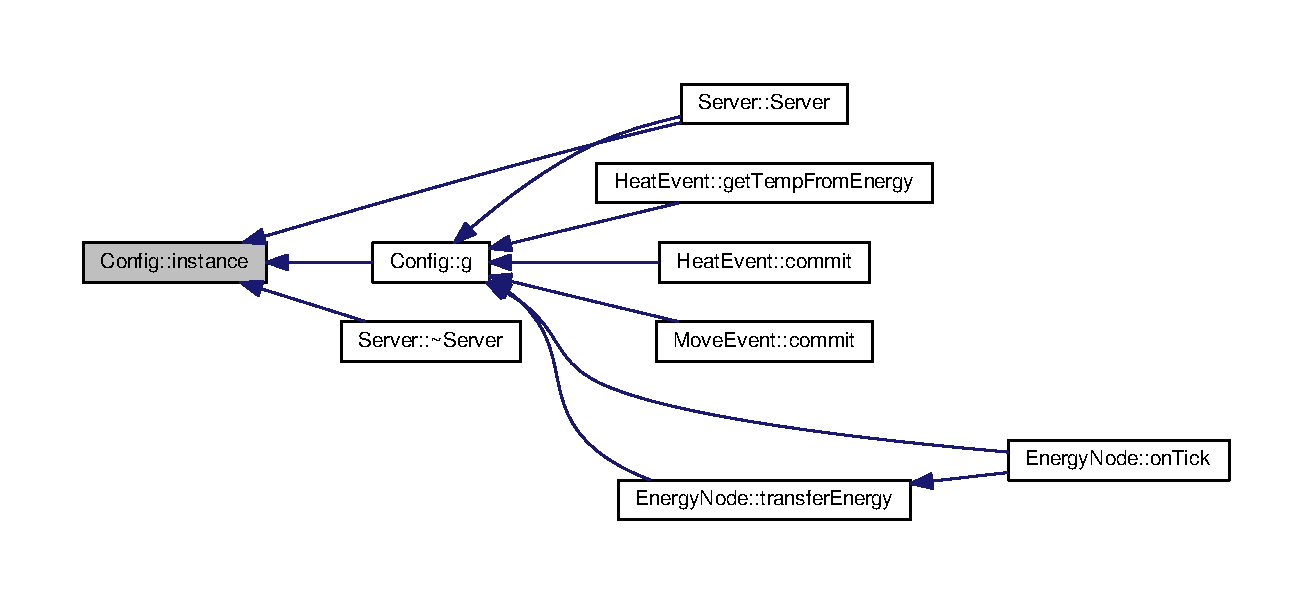
\includegraphics[width=350pt]{class_config_abf1d4539011ef83cac0fef2ac864a3a9_icgraph}
\end{center}
\end{figure}


\hypertarget{class_config_add4ebd0c89505c9b5368f03264555606}{\index{Config@{Config}!load@{load}}
\index{load@{load}!Config@{Config}}
\subsubsection[{load}]{\setlength{\rightskip}{0pt plus 5cm}void Config\-::load (
\begin{DoxyParamCaption}
{}
\end{DoxyParamCaption}
)}}\label{class_config_add4ebd0c89505c9b5368f03264555606}
\hypertarget{class_config_ae7e68962f22a2c965a61702de1c637db}{\index{Config@{Config}!save@{save}}
\index{save@{save}!Config@{Config}}
\subsubsection[{save}]{\setlength{\rightskip}{0pt plus 5cm}void Config\-::save (
\begin{DoxyParamCaption}
{}
\end{DoxyParamCaption}
)}}\label{class_config_ae7e68962f22a2c965a61702de1c637db}


Here is the call graph for this function\-:
\nopagebreak
\begin{figure}[H]
\begin{center}
\leavevmode
\includegraphics[width=296pt]{class_config_ae7e68962f22a2c965a61702de1c637db_cgraph}
\end{center}
\end{figure}


\hypertarget{class_config_a006701bd126aa5809b3a15e75c63bfb6}{\index{Config@{Config}!tree@{tree}}
\index{tree@{tree}!Config@{Config}}
\subsubsection[{tree}]{\setlength{\rightskip}{0pt plus 5cm}ptree \& Config\-::tree (
\begin{DoxyParamCaption}
{}
\end{DoxyParamCaption}
)}}\label{class_config_a006701bd126aa5809b3a15e75c63bfb6}


Here is the caller graph for this function\-:
\nopagebreak
\begin{figure}[H]
\begin{center}
\leavevmode
\includegraphics[width=350pt]{class_config_a006701bd126aa5809b3a15e75c63bfb6_icgraph}
\end{center}
\end{figure}




The documentation for this class was generated from the following files\-:\begin{DoxyCompactItemize}
\item 
/home/travis/build/bender-\/wardrobe/\-Recast/src/headers/io/configs/\hyperlink{_config_8hpp}{Config.\-hpp}\item 
/home/travis/build/bender-\/wardrobe/\-Recast/src/core/io/configs/\hyperlink{_config_8cpp}{Config.\-cpp}\end{DoxyCompactItemize}

\hypertarget{struct_coord}{\section{Coord Struct Reference}
\label{struct_coord}\index{Coord@{Coord}}
}


{\ttfamily \#include $<$Coord.\-hpp$>$}



Inheritance diagram for Coord\-:
\nopagebreak
\begin{figure}[H]
\begin{center}
\leavevmode
\includegraphics[width=186pt]{struct_coord__inherit__graph}
\end{center}
\end{figure}


Collaboration diagram for Coord\-:
\nopagebreak
\begin{figure}[H]
\begin{center}
\leavevmode
\includegraphics[width=186pt]{struct_coord__coll__graph}
\end{center}
\end{figure}
\subsection*{Public Member Functions}
\begin{DoxyCompactItemize}
\item 
\hyperlink{struct_coord_a2ffbed495521bbc7fe0263c5dbc88dee}{Coord} (int value=0)
\end{DoxyCompactItemize}
\subsection*{Additional Inherited Members}


\subsection{Detailed Description}
Type. Represents coordinate in a space. 

\subsection{Constructor \& Destructor Documentation}
\hypertarget{struct_coord_a2ffbed495521bbc7fe0263c5dbc88dee}{\index{Coord@{Coord}!Coord@{Coord}}
\index{Coord@{Coord}!Coord@{Coord}}
\subsubsection[{Coord}]{\setlength{\rightskip}{0pt plus 5cm}Coord\-::\-Coord (
\begin{DoxyParamCaption}
\item[{int}]{value = {\ttfamily 0}}
\end{DoxyParamCaption}
)\hspace{0.3cm}{\ttfamily [inline]}}}\label{struct_coord_a2ffbed495521bbc7fe0263c5dbc88dee}


The documentation for this struct was generated from the following file\-:\begin{DoxyCompactItemize}
\item 
/home/travis/build/glitchless/\-Recast/src/headers/temperature-\/world/types/\hyperlink{_coord_8hpp}{Coord.\-hpp}\end{DoxyCompactItemize}

\hypertarget{class_debug_network_listener}{\section{Debug\-Network\-Listener Class Reference}
\label{class_debug_network_listener}\index{Debug\-Network\-Listener@{Debug\-Network\-Listener}}
}


{\ttfamily \#include $<$Network\-Listener.\-hpp$>$}



Inheritance diagram for Debug\-Network\-Listener\-:
\nopagebreak
\begin{figure}[H]
\begin{center}
\leavevmode
\includegraphics[width=194pt]{class_debug_network_listener__inherit__graph}
\end{center}
\end{figure}


Collaboration diagram for Debug\-Network\-Listener\-:
\nopagebreak
\begin{figure}[H]
\begin{center}
\leavevmode
\includegraphics[width=194pt]{class_debug_network_listener__coll__graph}
\end{center}
\end{figure}
\subsection*{Public Member Functions}
\begin{DoxyCompactItemize}
\item 
char $\ast$ \hyperlink{class_debug_network_listener_a320f61476c1bacc235594731e39c51ff}{on\-Packet} (char $\ast$request, \hyperlink{class_i_command_sender}{I\-Command\-Sender} $\ast$sender)
\end{DoxyCompactItemize}
\subsection*{Additional Inherited Members}


\subsection{Member Function Documentation}
\hypertarget{class_debug_network_listener_a320f61476c1bacc235594731e39c51ff}{\index{Debug\-Network\-Listener@{Debug\-Network\-Listener}!on\-Packet@{on\-Packet}}
\index{on\-Packet@{on\-Packet}!DebugNetworkListener@{Debug\-Network\-Listener}}
\subsubsection[{on\-Packet}]{\setlength{\rightskip}{0pt plus 5cm}char$\ast$ Debug\-Network\-Listener\-::on\-Packet (
\begin{DoxyParamCaption}
\item[{char $\ast$}]{request, }
\item[{{\bf I\-Command\-Sender} $\ast$}]{sender}
\end{DoxyParamCaption}
)\hspace{0.3cm}{\ttfamily [inline]}, {\ttfamily [virtual]}}}\label{class_debug_network_listener_a320f61476c1bacc235594731e39c51ff}


Implements \hyperlink{class_network_listener_a721846b67227e7b3ac96c3d7d7065655}{Network\-Listener}.



Here is the call graph for this function\-:
\nopagebreak
\begin{figure}[H]
\begin{center}
\leavevmode
\includegraphics[width=350pt]{class_debug_network_listener_a320f61476c1bacc235594731e39c51ff_cgraph}
\end{center}
\end{figure}




The documentation for this class was generated from the following file\-:\begin{DoxyCompactItemize}
\item 
/home/travis/build/glitchless/\-Recast/src/headers/io/network/\hyperlink{_network_listener_8hpp}{Network\-Listener.\-hpp}\end{DoxyCompactItemize}

\hypertarget{class_energy_node}{\section{Energy\-Node Class Reference}
\label{class_energy_node}\index{Energy\-Node@{Energy\-Node}}
}


{\ttfamily \#include $<$Energy\-Node.\-hpp$>$}



Inheritance diagram for Energy\-Node\-:
\nopagebreak
\begin{figure}[H]
\begin{center}
\leavevmode
\includegraphics[height=550pt]{class_energy_node__inherit__graph}
\end{center}
\end{figure}


Collaboration diagram for Energy\-Node\-:
\nopagebreak
\begin{figure}[H]
\begin{center}
\leavevmode
\includegraphics[width=200pt]{class_energy_node__coll__graph}
\end{center}
\end{figure}
\subsection*{Public Member Functions}
\begin{DoxyCompactItemize}
\item 
\hyperlink{class_energy_node_a607a0f6e31ff16ff882440119739ad66}{Energy\-Node} (float \hyperlink{class_spell_node_a916f2a709a674dd2a61530b6acc339cc}{x}, float \hyperlink{class_spell_node_a754d80fd0fd82dbc12443b5f277b9fb4}{y}, float \hyperlink{class_spell_node_aff090331ff1bd816a22e974a50c1a180}{z}, float \hyperlink{class_energy_node_ac2cd46828178316e24f339489f553852}{energy})
\item 
\hyperlink{class_energy_node_aa1a37a897c0e95fa3c153ea6993c5237}{Energy\-Node} (\hyperlink{_spell_node_8hpp_acac9cbaeea226ed297804c012dc12b16}{Node\-Type} \hyperlink{class_spell_node_ae897f4f135608a9c71948b5f703aeb99}{type}, float \hyperlink{class_spell_node_a916f2a709a674dd2a61530b6acc339cc}{x}, float \hyperlink{class_spell_node_a754d80fd0fd82dbc12443b5f277b9fb4}{y}, float \hyperlink{class_spell_node_aff090331ff1bd816a22e974a50c1a180}{z}, float \hyperlink{class_energy_node_ac2cd46828178316e24f339489f553852}{energy})
\item 
virtual bool \hyperlink{class_energy_node_a3a215be078964713e490198ee311d70f}{is\-Energy\-Node} ()
\item 
float \hyperlink{class_energy_node_aac6faa1fe6389c0f9ee63611cd322245}{get\-Energy} () const 
\item 
virtual float \hyperlink{class_energy_node_a04b3fe7a8aa49157a5c66ee8e25cfb3b}{transfer\-Energy} (\hyperlink{class_spell_node}{Spell\-Node} $\ast$from, float count)
\end{DoxyCompactItemize}
\subsection*{Protected Member Functions}
\begin{DoxyCompactItemize}
\item 
virtual void \hyperlink{class_energy_node_ab52474e2e15ff2af2d969b6a88a778f7}{on\-Tick} (\hyperlink{class_i_event_listener}{I\-Event\-Listener} \&listener, \hyperlink{class_spell_node}{Spell\-Node} $\ast$callable)
\end{DoxyCompactItemize}
\subsection*{Protected Attributes}
\begin{DoxyCompactItemize}
\item 
float \hyperlink{class_energy_node_ac2cd46828178316e24f339489f553852}{energy} = 0
\end{DoxyCompactItemize}
\subsection*{Additional Inherited Members}


\subsection{Constructor \& Destructor Documentation}
\hypertarget{class_energy_node_a607a0f6e31ff16ff882440119739ad66}{\index{Energy\-Node@{Energy\-Node}!Energy\-Node@{Energy\-Node}}
\index{Energy\-Node@{Energy\-Node}!EnergyNode@{Energy\-Node}}
\subsubsection[{Energy\-Node}]{\setlength{\rightskip}{0pt plus 5cm}Energy\-Node\-::\-Energy\-Node (
\begin{DoxyParamCaption}
\item[{float}]{x, }
\item[{float}]{y, }
\item[{float}]{z, }
\item[{float}]{energy}
\end{DoxyParamCaption}
)\hspace{0.3cm}{\ttfamily [inline]}}}\label{class_energy_node_a607a0f6e31ff16ff882440119739ad66}
\hypertarget{class_energy_node_aa1a37a897c0e95fa3c153ea6993c5237}{\index{Energy\-Node@{Energy\-Node}!Energy\-Node@{Energy\-Node}}
\index{Energy\-Node@{Energy\-Node}!EnergyNode@{Energy\-Node}}
\subsubsection[{Energy\-Node}]{\setlength{\rightskip}{0pt plus 5cm}Energy\-Node\-::\-Energy\-Node (
\begin{DoxyParamCaption}
\item[{{\bf Node\-Type}}]{type, }
\item[{float}]{x, }
\item[{float}]{y, }
\item[{float}]{z, }
\item[{float}]{energy}
\end{DoxyParamCaption}
)\hspace{0.3cm}{\ttfamily [inline]}}}\label{class_energy_node_aa1a37a897c0e95fa3c153ea6993c5237}


\subsection{Member Function Documentation}
\hypertarget{class_energy_node_aac6faa1fe6389c0f9ee63611cd322245}{\index{Energy\-Node@{Energy\-Node}!get\-Energy@{get\-Energy}}
\index{get\-Energy@{get\-Energy}!EnergyNode@{Energy\-Node}}
\subsubsection[{get\-Energy}]{\setlength{\rightskip}{0pt plus 5cm}float Energy\-Node\-::get\-Energy (
\begin{DoxyParamCaption}
{}
\end{DoxyParamCaption}
) const\hspace{0.3cm}{\ttfamily [inline]}}}\label{class_energy_node_aac6faa1fe6389c0f9ee63611cd322245}


Here is the caller graph for this function\-:
\nopagebreak
\begin{figure}[H]
\begin{center}
\leavevmode
\includegraphics[width=344pt]{class_energy_node_aac6faa1fe6389c0f9ee63611cd322245_icgraph}
\end{center}
\end{figure}


\hypertarget{class_energy_node_a3a215be078964713e490198ee311d70f}{\index{Energy\-Node@{Energy\-Node}!is\-Energy\-Node@{is\-Energy\-Node}}
\index{is\-Energy\-Node@{is\-Energy\-Node}!EnergyNode@{Energy\-Node}}
\subsubsection[{is\-Energy\-Node}]{\setlength{\rightskip}{0pt plus 5cm}virtual bool Energy\-Node\-::is\-Energy\-Node (
\begin{DoxyParamCaption}
{}
\end{DoxyParamCaption}
)\hspace{0.3cm}{\ttfamily [inline]}, {\ttfamily [virtual]}}}\label{class_energy_node_a3a215be078964713e490198ee311d70f}


Reimplemented from \hyperlink{class_spell_node_aa697b780e010dea8deb78eae8f61e36f}{Spell\-Node}.

\hypertarget{class_energy_node_ab52474e2e15ff2af2d969b6a88a778f7}{\index{Energy\-Node@{Energy\-Node}!on\-Tick@{on\-Tick}}
\index{on\-Tick@{on\-Tick}!EnergyNode@{Energy\-Node}}
\subsubsection[{on\-Tick}]{\setlength{\rightskip}{0pt plus 5cm}void Energy\-Node\-::on\-Tick (
\begin{DoxyParamCaption}
\item[{{\bf I\-Event\-Listener} \&}]{listener, }
\item[{{\bf Spell\-Node} $\ast$}]{callable}
\end{DoxyParamCaption}
)\hspace{0.3cm}{\ttfamily [protected]}, {\ttfamily [virtual]}}}\label{class_energy_node_ab52474e2e15ff2af2d969b6a88a778f7}
Каждый тик мы рапределяем почти равномерно энергию между всеми дочерними нодами. Энергия переливается только в том случае, если её где-\/то меньше чем в текущей ноде. По умолчанию размер пакета = (Энергия текущего пакета -\/ Энергия дочернего пакета) $\ast$ 0.\-1 (10\% от транзакции) Каждая передача энергии сопровождается потерей. В контексте проекта это называется налог на энергию (energy tax). Это приводит к тому, что энергия не вечна и рано или поздно пропадет из плетения.


\begin{DoxyParams}{Parameters}
{\em listener} & Вся передача событий из заклинания наружу происходит с помощью Event'ов \\
\hline
{\em callable} & Вызывающая нода. Пока не пригождается, но мало ли. Может быть N\-U\-L\-L \\
\hline
\end{DoxyParams}


Reimplemented from \hyperlink{class_spell_node_a0e8d39e7ebc6c7bd9e52eaf1be213af8}{Spell\-Node}.



Here is the call graph for this function\-:
\nopagebreak
\begin{figure}[H]
\begin{center}
\leavevmode
\includegraphics[width=350pt]{class_energy_node_ab52474e2e15ff2af2d969b6a88a778f7_cgraph}
\end{center}
\end{figure}


\hypertarget{class_energy_node_a04b3fe7a8aa49157a5c66ee8e25cfb3b}{\index{Energy\-Node@{Energy\-Node}!transfer\-Energy@{transfer\-Energy}}
\index{transfer\-Energy@{transfer\-Energy}!EnergyNode@{Energy\-Node}}
\subsubsection[{transfer\-Energy}]{\setlength{\rightskip}{0pt plus 5cm}float Energy\-Node\-::transfer\-Energy (
\begin{DoxyParamCaption}
\item[{{\bf Spell\-Node} $\ast$}]{from, }
\item[{float}]{count}
\end{DoxyParamCaption}
)\hspace{0.3cm}{\ttfamily [virtual]}}}\label{class_energy_node_a04b3fe7a8aa49157a5c66ee8e25cfb3b}


Here is the call graph for this function\-:
\nopagebreak
\begin{figure}[H]
\begin{center}
\leavevmode
\includegraphics[width=350pt]{class_energy_node_a04b3fe7a8aa49157a5c66ee8e25cfb3b_cgraph}
\end{center}
\end{figure}




Here is the caller graph for this function\-:
\nopagebreak
\begin{figure}[H]
\begin{center}
\leavevmode
\includegraphics[width=350pt]{class_energy_node_a04b3fe7a8aa49157a5c66ee8e25cfb3b_icgraph}
\end{center}
\end{figure}




\subsection{Member Data Documentation}
\hypertarget{class_energy_node_ac2cd46828178316e24f339489f553852}{\index{Energy\-Node@{Energy\-Node}!energy@{energy}}
\index{energy@{energy}!EnergyNode@{Energy\-Node}}
\subsubsection[{energy}]{\setlength{\rightskip}{0pt plus 5cm}float Energy\-Node\-::energy = 0\hspace{0.3cm}{\ttfamily [protected]}}}\label{class_energy_node_ac2cd46828178316e24f339489f553852}


The documentation for this class was generated from the following files\-:\begin{DoxyCompactItemize}
\item 
/home/travis/build/bender-\/wardrobe/\-Recast/src/headers/spells/nodes/\hyperlink{_energy_node_8hpp}{Energy\-Node.\-hpp}\item 
/home/travis/build/bender-\/wardrobe/\-Recast/src/spell/nodes/\hyperlink{_energy_node_8cpp}{Energy\-Node.\-cpp}\end{DoxyCompactItemize}

\hypertarget{class_generatable_chunked_temperature_world}{\section{Generatable\-Chunked\-Temperature\-World Class Reference}
\label{class_generatable_chunked_temperature_world}\index{Generatable\-Chunked\-Temperature\-World@{Generatable\-Chunked\-Temperature\-World}}
}


{\ttfamily \#include $<$Generatable\-Chunked\-Temperature\-World.\-hpp$>$}



Inheritance diagram for Generatable\-Chunked\-Temperature\-World\-:
\nopagebreak
\begin{figure}[H]
\begin{center}
\leavevmode
\includegraphics[height=550pt]{class_generatable_chunked_temperature_world__inherit__graph}
\end{center}
\end{figure}


Collaboration diagram for Generatable\-Chunked\-Temperature\-World\-:
\nopagebreak
\begin{figure}[H]
\begin{center}
\leavevmode
\includegraphics[height=550pt]{class_generatable_chunked_temperature_world__coll__graph}
\end{center}
\end{figure}
\subsection*{Public Member Functions}
\begin{DoxyCompactItemize}
\item 
\hyperlink{class_generatable_chunked_temperature_world_ac452b01dbd1b3d78b265007a96b2d1f0}{Generatable\-Chunked\-Temperature\-World} (\hyperlink{namespace_generatable_chunked_temperature_world_typedefs_a07d38658571f8f09839bc1bc8b105107}{Generatable\-Chunked\-Temperature\-World\-Typedefs\-::\-Need\-Chunk\-Fn} need\-Chunk\-Fn, \hyperlink{namespace_generatable_chunked_temperature_world_typedefs_a719e4469a105a21a76ed22274639c03a}{Generatable\-Chunked\-Temperature\-World\-Typedefs\-::\-Make\-Chunk\-Fn} make\-Chunk\-Fn)
\item 
bool \hyperlink{class_generatable_chunked_temperature_world_ad8ebd44d64067e9920d76d46af1b83e2}{has\-Or\-Is\-Generatable\-Chunk} (\hyperlink{struct_coord}{Coord} x, \hyperlink{struct_coord}{Coord} y, \hyperlink{struct_coord}{Coord} z) const noexceptoverride
\item 
std\-::shared\-\_\-ptr\\*
$<$ \hyperlink{class_i_temperature_world_boundable}{I\-Temperature\-World\-Boundable}\\*
$<$ \hyperlink{class_i_temperature_world}{I\-Temperature\-World} $>$ $>$ \hyperlink{class_generatable_chunked_temperature_world_ad5455846504972898e622f9437846f8c}{get\-Or\-Generate\-Chunk} (\hyperlink{struct_coord}{Coord} x, \hyperlink{struct_coord}{Coord} y, \hyperlink{struct_coord}{Coord} z) override
\item 
void \hyperlink{class_generatable_chunked_temperature_world_af1a6752db0e722e8649ddb4c7e1ea8fa}{add\-Chunk} (std\-::shared\-\_\-ptr$<$ \hyperlink{class_i_temperature_world_boundable}{I\-Temperature\-World\-Boundable}$<$ \hyperlink{class_i_temperature_world}{I\-Temperature\-World} $>$$>$ chunk) override
\item 
void \hyperlink{class_generatable_chunked_temperature_world_a42c646343bb79dcdeb9f96e6aa06cbec}{remove\-Chunk} (std\-::shared\-\_\-ptr$<$ \hyperlink{class_i_temperature_world_boundable}{I\-Temperature\-World\-Boundable}$<$ \hyperlink{class_i_temperature_world}{I\-Temperature\-World} $>$$>$ chunk) override
\item 
void \hyperlink{class_generatable_chunked_temperature_world_aa0b55baf21d9605af04d8fef99f9fbd8}{on\-Chunk\-Add} (\hyperlink{class_i_temperature_world_chunkable_observable_mixin_a777c50f4a4ca0b3f7cd6bc02b87bb883}{On\-Chunk\-Event\-Fn} func) override
\item 
void \hyperlink{class_generatable_chunked_temperature_world_a4416f9f9ea400e540b1214b053692760}{on\-Chunk\-Remove} (\hyperlink{class_i_temperature_world_chunkable_observable_mixin_a777c50f4a4ca0b3f7cd6bc02b87bb883}{On\-Chunk\-Event\-Fn} func) override
\end{DoxyCompactItemize}
\subsection*{Protected Attributes}
\begin{DoxyCompactItemize}
\item 
\hyperlink{namespace_generatable_chunked_temperature_world_typedefs_a07d38658571f8f09839bc1bc8b105107}{Generatable\-Chunked\-Temperature\-World\-Typedefs\-::\-Need\-Chunk\-Fn} \hyperlink{class_generatable_chunked_temperature_world_a9159830777efdcfab20bd6f1e84eda42}{\-\_\-need\-Chunk\-Fn}
\item 
\hyperlink{namespace_generatable_chunked_temperature_world_typedefs_a719e4469a105a21a76ed22274639c03a}{Generatable\-Chunked\-Temperature\-World\-Typedefs\-::\-Make\-Chunk\-Fn} \hyperlink{class_generatable_chunked_temperature_world_ad1573a4224ea6bbe88843ed82f26e107}{\-\_\-make\-Chunk\-Fn}
\item 
std\-::list$<$ \hyperlink{class_i_temperature_world_chunkable_observable_mixin_a777c50f4a4ca0b3f7cd6bc02b87bb883}{On\-Chunk\-Event\-Fn} $>$ \hyperlink{class_generatable_chunked_temperature_world_a4d8bd2602e4563b1f347e967bc1d3f23}{\-\_\-on\-Chunk\-Add\-Listeners}
\item 
std\-::list$<$ \hyperlink{class_i_temperature_world_chunkable_observable_mixin_a777c50f4a4ca0b3f7cd6bc02b87bb883}{On\-Chunk\-Event\-Fn} $>$ \hyperlink{class_generatable_chunked_temperature_world_a4f5ce92a800ce903982033724d025e09}{\-\_\-on\-Chunk\-Remove\-Listeners}
\end{DoxyCompactItemize}
\subsection*{Additional Inherited Members}


\subsection{Detailed Description}
Implementation of temperature world divided by chunks. It's backed by {\ttfamily std\-::list}. It will create new chunk if client accesses temperature of point in non-\/existing chunk. 

\subsection{Constructor \& Destructor Documentation}
\hypertarget{class_generatable_chunked_temperature_world_ac452b01dbd1b3d78b265007a96b2d1f0}{\index{Generatable\-Chunked\-Temperature\-World@{Generatable\-Chunked\-Temperature\-World}!Generatable\-Chunked\-Temperature\-World@{Generatable\-Chunked\-Temperature\-World}}
\index{Generatable\-Chunked\-Temperature\-World@{Generatable\-Chunked\-Temperature\-World}!GeneratableChunkedTemperatureWorld@{Generatable\-Chunked\-Temperature\-World}}
\subsubsection[{Generatable\-Chunked\-Temperature\-World}]{\setlength{\rightskip}{0pt plus 5cm}Generatable\-Chunked\-Temperature\-World\-::\-Generatable\-Chunked\-Temperature\-World (
\begin{DoxyParamCaption}
\item[{{\bf Generatable\-Chunked\-Temperature\-World\-Typedefs\-::\-Need\-Chunk\-Fn}}]{need\-Chunk\-Fn, }
\item[{{\bf Generatable\-Chunked\-Temperature\-World\-Typedefs\-::\-Make\-Chunk\-Fn}}]{make\-Chunk\-Fn}
\end{DoxyParamCaption}
)}}\label{class_generatable_chunked_temperature_world_ac452b01dbd1b3d78b265007a96b2d1f0}


\subsection{Member Function Documentation}
\hypertarget{class_generatable_chunked_temperature_world_af1a6752db0e722e8649ddb4c7e1ea8fa}{\index{Generatable\-Chunked\-Temperature\-World@{Generatable\-Chunked\-Temperature\-World}!add\-Chunk@{add\-Chunk}}
\index{add\-Chunk@{add\-Chunk}!GeneratableChunkedTemperatureWorld@{Generatable\-Chunked\-Temperature\-World}}
\subsubsection[{add\-Chunk}]{\setlength{\rightskip}{0pt plus 5cm}void Generatable\-Chunked\-Temperature\-World\-::add\-Chunk (
\begin{DoxyParamCaption}
\item[{std\-::shared\-\_\-ptr$<$ {\bf I\-Temperature\-World\-Boundable}$<$ {\bf I\-Temperature\-World} $>$$>$}]{chunk}
\end{DoxyParamCaption}
)\hspace{0.3cm}{\ttfamily [override]}, {\ttfamily [virtual]}}}\label{class_generatable_chunked_temperature_world_af1a6752db0e722e8649ddb4c7e1ea8fa}
Adds a chunk to this temperature world.


\begin{DoxyParams}{Parameters}
{\em chunk} & Chunk to add. \\
\hline
\end{DoxyParams}


Reimplemented from \hyperlink{class_chunked_temperature_world_a5f9a3a143baf0c0238427926aef77f65}{Chunked\-Temperature\-World}.



Reimplemented in \hyperlink{class_scaling_generatable_chunked_temperature_world_a5ec1b1a2a5e058bf57bd7918fcc5a35b}{Scaling\-Generatable\-Chunked\-Temperature\-World}.



Here is the call graph for this function\-:
\nopagebreak
\begin{figure}[H]
\begin{center}
\leavevmode
\includegraphics[width=350pt]{class_generatable_chunked_temperature_world_af1a6752db0e722e8649ddb4c7e1ea8fa_cgraph}
\end{center}
\end{figure}




Here is the caller graph for this function\-:
\nopagebreak
\begin{figure}[H]
\begin{center}
\leavevmode
\includegraphics[width=350pt]{class_generatable_chunked_temperature_world_af1a6752db0e722e8649ddb4c7e1ea8fa_icgraph}
\end{center}
\end{figure}


\hypertarget{class_generatable_chunked_temperature_world_ad5455846504972898e622f9437846f8c}{\index{Generatable\-Chunked\-Temperature\-World@{Generatable\-Chunked\-Temperature\-World}!get\-Or\-Generate\-Chunk@{get\-Or\-Generate\-Chunk}}
\index{get\-Or\-Generate\-Chunk@{get\-Or\-Generate\-Chunk}!GeneratableChunkedTemperatureWorld@{Generatable\-Chunked\-Temperature\-World}}
\subsubsection[{get\-Or\-Generate\-Chunk}]{\setlength{\rightskip}{0pt plus 5cm}shared\-\_\-ptr$<$ {\bf I\-Temperature\-World\-Boundable}$<$ {\bf I\-Temperature\-World} $>$ $>$ Generatable\-Chunked\-Temperature\-World\-::get\-Or\-Generate\-Chunk (
\begin{DoxyParamCaption}
\item[{{\bf Coord}}]{x, }
\item[{{\bf Coord}}]{y, }
\item[{{\bf Coord}}]{z}
\end{DoxyParamCaption}
)\hspace{0.3cm}{\ttfamily [override]}, {\ttfamily [virtual]}}}\label{class_generatable_chunked_temperature_world_ad5455846504972898e622f9437846f8c}
Retrieves chunk which holds this point. If chunk doesn't exist, the method will generate chunk if it's possible.


\begin{DoxyParams}{Parameters}
{\em x} & X coordinate. \\
\hline
{\em y} & Y coordinate. \\
\hline
{\em z} & Z coordinate. \\
\hline
\end{DoxyParams}
\begin{DoxyReturn}{Returns}
Chunk at the point. 
\end{DoxyReturn}


Implements \hyperlink{class_i_temperature_world_chunkable_generatable_mixin_a1144edcb06ba318422be96ee5f8b139d}{I\-Temperature\-World\-Chunkable\-Generatable\-Mixin}.



Here is the call graph for this function\-:
\nopagebreak
\begin{figure}[H]
\begin{center}
\leavevmode
\includegraphics[width=350pt]{class_generatable_chunked_temperature_world_ad5455846504972898e622f9437846f8c_cgraph}
\end{center}
\end{figure}


\hypertarget{class_generatable_chunked_temperature_world_ad8ebd44d64067e9920d76d46af1b83e2}{\index{Generatable\-Chunked\-Temperature\-World@{Generatable\-Chunked\-Temperature\-World}!has\-Or\-Is\-Generatable\-Chunk@{has\-Or\-Is\-Generatable\-Chunk}}
\index{has\-Or\-Is\-Generatable\-Chunk@{has\-Or\-Is\-Generatable\-Chunk}!GeneratableChunkedTemperatureWorld@{Generatable\-Chunked\-Temperature\-World}}
\subsubsection[{has\-Or\-Is\-Generatable\-Chunk}]{\setlength{\rightskip}{0pt plus 5cm}bool Generatable\-Chunked\-Temperature\-World\-::has\-Or\-Is\-Generatable\-Chunk (
\begin{DoxyParamCaption}
\item[{{\bf Coord}}]{x, }
\item[{{\bf Coord}}]{y, }
\item[{{\bf Coord}}]{z}
\end{DoxyParamCaption}
) const\hspace{0.3cm}{\ttfamily [override]}, {\ttfamily [virtual]}, {\ttfamily [noexcept]}}}\label{class_generatable_chunked_temperature_world_ad8ebd44d64067e9920d76d46af1b83e2}
Tells whether the chunk which holds this point exists. If chunk doesn't exist, the method will tell whether it will generated on {\ttfamily get\-Or\-Generate\-Chunk} call. This method doesn't throw exceptions.


\begin{DoxyParams}{Parameters}
{\em x} & X coordinate. \\
\hline
{\em y} & Y coordinate. \\
\hline
{\em z} & Z coordinate. \\
\hline
\end{DoxyParams}
\begin{DoxyReturn}{Returns}
True if chunk exists. 
\end{DoxyReturn}


Implements \hyperlink{class_i_temperature_world_chunkable_generatable_mixin_a015be90684c10d61cc962439b3ed71ef}{I\-Temperature\-World\-Chunkable\-Generatable\-Mixin}.

\hypertarget{class_generatable_chunked_temperature_world_aa0b55baf21d9605af04d8fef99f9fbd8}{\index{Generatable\-Chunked\-Temperature\-World@{Generatable\-Chunked\-Temperature\-World}!on\-Chunk\-Add@{on\-Chunk\-Add}}
\index{on\-Chunk\-Add@{on\-Chunk\-Add}!GeneratableChunkedTemperatureWorld@{Generatable\-Chunked\-Temperature\-World}}
\subsubsection[{on\-Chunk\-Add}]{\setlength{\rightskip}{0pt plus 5cm}void Generatable\-Chunked\-Temperature\-World\-::on\-Chunk\-Add (
\begin{DoxyParamCaption}
\item[{{\bf On\-Chunk\-Event\-Fn}}]{func}
\end{DoxyParamCaption}
)\hspace{0.3cm}{\ttfamily [override]}, {\ttfamily [virtual]}}}\label{class_generatable_chunked_temperature_world_aa0b55baf21d9605af04d8fef99f9fbd8}
Subscribes listener to chunk add events.


\begin{DoxyParams}{Parameters}
{\em func} & Listener. \\
\hline
\end{DoxyParams}


Implements \hyperlink{class_i_temperature_world_chunkable_observable_mixin_a5bafba4f885aa5ae4cab3133d75d45d1}{I\-Temperature\-World\-Chunkable\-Observable\-Mixin}.

\hypertarget{class_generatable_chunked_temperature_world_a4416f9f9ea400e540b1214b053692760}{\index{Generatable\-Chunked\-Temperature\-World@{Generatable\-Chunked\-Temperature\-World}!on\-Chunk\-Remove@{on\-Chunk\-Remove}}
\index{on\-Chunk\-Remove@{on\-Chunk\-Remove}!GeneratableChunkedTemperatureWorld@{Generatable\-Chunked\-Temperature\-World}}
\subsubsection[{on\-Chunk\-Remove}]{\setlength{\rightskip}{0pt plus 5cm}void Generatable\-Chunked\-Temperature\-World\-::on\-Chunk\-Remove (
\begin{DoxyParamCaption}
\item[{{\bf On\-Chunk\-Event\-Fn}}]{func}
\end{DoxyParamCaption}
)\hspace{0.3cm}{\ttfamily [override]}, {\ttfamily [virtual]}}}\label{class_generatable_chunked_temperature_world_a4416f9f9ea400e540b1214b053692760}
Subscribes listener to chunk remove events.


\begin{DoxyParams}{Parameters}
{\em func} & Listener. \\
\hline
\end{DoxyParams}


Implements \hyperlink{class_i_temperature_world_chunkable_observable_mixin_a85cfb47d07c70183d1c4da81a91da599}{I\-Temperature\-World\-Chunkable\-Observable\-Mixin}.

\hypertarget{class_generatable_chunked_temperature_world_a42c646343bb79dcdeb9f96e6aa06cbec}{\index{Generatable\-Chunked\-Temperature\-World@{Generatable\-Chunked\-Temperature\-World}!remove\-Chunk@{remove\-Chunk}}
\index{remove\-Chunk@{remove\-Chunk}!GeneratableChunkedTemperatureWorld@{Generatable\-Chunked\-Temperature\-World}}
\subsubsection[{remove\-Chunk}]{\setlength{\rightskip}{0pt plus 5cm}void Generatable\-Chunked\-Temperature\-World\-::remove\-Chunk (
\begin{DoxyParamCaption}
\item[{std\-::shared\-\_\-ptr$<$ {\bf I\-Temperature\-World\-Boundable}$<$ {\bf I\-Temperature\-World} $>$$>$}]{chunk}
\end{DoxyParamCaption}
)\hspace{0.3cm}{\ttfamily [override]}, {\ttfamily [virtual]}}}\label{class_generatable_chunked_temperature_world_a42c646343bb79dcdeb9f96e6aa06cbec}
Removes chunk from this temperature world.


\begin{DoxyParams}{Parameters}
{\em chunk} & Chunk to remove. \\
\hline
\end{DoxyParams}


Reimplemented from \hyperlink{class_chunked_temperature_world_a623c1f5efe7aa84d428ba58365ee775a}{Chunked\-Temperature\-World}.



Reimplemented in \hyperlink{class_scaling_generatable_chunked_temperature_world_ac3ae4d696d934b925076eeab88658978}{Scaling\-Generatable\-Chunked\-Temperature\-World}.



Here is the call graph for this function\-:
\nopagebreak
\begin{figure}[H]
\begin{center}
\leavevmode
\includegraphics[width=350pt]{class_generatable_chunked_temperature_world_a42c646343bb79dcdeb9f96e6aa06cbec_cgraph}
\end{center}
\end{figure}




Here is the caller graph for this function\-:
\nopagebreak
\begin{figure}[H]
\begin{center}
\leavevmode
\includegraphics[width=350pt]{class_generatable_chunked_temperature_world_a42c646343bb79dcdeb9f96e6aa06cbec_icgraph}
\end{center}
\end{figure}




\subsection{Member Data Documentation}
\hypertarget{class_generatable_chunked_temperature_world_ad1573a4224ea6bbe88843ed82f26e107}{\index{Generatable\-Chunked\-Temperature\-World@{Generatable\-Chunked\-Temperature\-World}!\-\_\-make\-Chunk\-Fn@{\-\_\-make\-Chunk\-Fn}}
\index{\-\_\-make\-Chunk\-Fn@{\-\_\-make\-Chunk\-Fn}!GeneratableChunkedTemperatureWorld@{Generatable\-Chunked\-Temperature\-World}}
\subsubsection[{\-\_\-make\-Chunk\-Fn}]{\setlength{\rightskip}{0pt plus 5cm}{\bf Generatable\-Chunked\-Temperature\-World\-Typedefs\-::\-Make\-Chunk\-Fn} Generatable\-Chunked\-Temperature\-World\-::\-\_\-make\-Chunk\-Fn\hspace{0.3cm}{\ttfamily [protected]}}}\label{class_generatable_chunked_temperature_world_ad1573a4224ea6bbe88843ed82f26e107}
\hypertarget{class_generatable_chunked_temperature_world_a9159830777efdcfab20bd6f1e84eda42}{\index{Generatable\-Chunked\-Temperature\-World@{Generatable\-Chunked\-Temperature\-World}!\-\_\-need\-Chunk\-Fn@{\-\_\-need\-Chunk\-Fn}}
\index{\-\_\-need\-Chunk\-Fn@{\-\_\-need\-Chunk\-Fn}!GeneratableChunkedTemperatureWorld@{Generatable\-Chunked\-Temperature\-World}}
\subsubsection[{\-\_\-need\-Chunk\-Fn}]{\setlength{\rightskip}{0pt plus 5cm}{\bf Generatable\-Chunked\-Temperature\-World\-Typedefs\-::\-Need\-Chunk\-Fn} Generatable\-Chunked\-Temperature\-World\-::\-\_\-need\-Chunk\-Fn\hspace{0.3cm}{\ttfamily [protected]}}}\label{class_generatable_chunked_temperature_world_a9159830777efdcfab20bd6f1e84eda42}
\hypertarget{class_generatable_chunked_temperature_world_a4d8bd2602e4563b1f347e967bc1d3f23}{\index{Generatable\-Chunked\-Temperature\-World@{Generatable\-Chunked\-Temperature\-World}!\-\_\-on\-Chunk\-Add\-Listeners@{\-\_\-on\-Chunk\-Add\-Listeners}}
\index{\-\_\-on\-Chunk\-Add\-Listeners@{\-\_\-on\-Chunk\-Add\-Listeners}!GeneratableChunkedTemperatureWorld@{Generatable\-Chunked\-Temperature\-World}}
\subsubsection[{\-\_\-on\-Chunk\-Add\-Listeners}]{\setlength{\rightskip}{0pt plus 5cm}std\-::list$<${\bf On\-Chunk\-Event\-Fn}$>$ Generatable\-Chunked\-Temperature\-World\-::\-\_\-on\-Chunk\-Add\-Listeners\hspace{0.3cm}{\ttfamily [protected]}}}\label{class_generatable_chunked_temperature_world_a4d8bd2602e4563b1f347e967bc1d3f23}
\hypertarget{class_generatable_chunked_temperature_world_a4f5ce92a800ce903982033724d025e09}{\index{Generatable\-Chunked\-Temperature\-World@{Generatable\-Chunked\-Temperature\-World}!\-\_\-on\-Chunk\-Remove\-Listeners@{\-\_\-on\-Chunk\-Remove\-Listeners}}
\index{\-\_\-on\-Chunk\-Remove\-Listeners@{\-\_\-on\-Chunk\-Remove\-Listeners}!GeneratableChunkedTemperatureWorld@{Generatable\-Chunked\-Temperature\-World}}
\subsubsection[{\-\_\-on\-Chunk\-Remove\-Listeners}]{\setlength{\rightskip}{0pt plus 5cm}std\-::list$<${\bf On\-Chunk\-Event\-Fn}$>$ Generatable\-Chunked\-Temperature\-World\-::\-\_\-on\-Chunk\-Remove\-Listeners\hspace{0.3cm}{\ttfamily [protected]}}}\label{class_generatable_chunked_temperature_world_a4f5ce92a800ce903982033724d025e09}


The documentation for this class was generated from the following files\-:\begin{DoxyCompactItemize}
\item 
/home/travis/build/bender-\/wardrobe/\-Recast/temperature-\/world/src/headers/temperature-\/world/implementation/\hyperlink{_generatable_chunked_temperature_world_8hpp}{Generatable\-Chunked\-Temperature\-World.\-hpp}\item 
/home/travis/build/bender-\/wardrobe/\-Recast/temperature-\/world/src/implementation/\hyperlink{_generatable_chunked_temperature_world_8cpp}{Generatable\-Chunked\-Temperature\-World.\-cpp}\end{DoxyCompactItemize}

\hypertarget{struct_generic_scalar}{\section{Generic\-Scalar$<$ T $>$ Struct Template Reference}
\label{struct_generic_scalar}\index{Generic\-Scalar$<$ T $>$@{Generic\-Scalar$<$ T $>$}}
}


{\ttfamily \#include $<$Generic\-Scalar.\-hpp$>$}



Collaboration diagram for Generic\-Scalar$<$ T $>$\-:
\nopagebreak
\begin{figure}[H]
\begin{center}
\leavevmode
\includegraphics[width=180pt]{struct_generic_scalar__coll__graph}
\end{center}
\end{figure}
\subsection*{Public Member Functions}
\begin{DoxyCompactItemize}
\item 
\hyperlink{struct_generic_scalar_aaabb6f012a3d829348c318e14b6dc551}{Generic\-Scalar} (T value)
\item 
\hyperlink{struct_generic_scalar_ae1346acd021b8f259e58723350d26729}{operator T} () const noexcept
\item 
\hyperlink{struct_generic_scalar_a4d146d4dce6f936e42211a6528cc9775}{operator T \&} () noexcept
\end{DoxyCompactItemize}
\subsection*{Protected Attributes}
\begin{DoxyCompactItemize}
\item 
T \hyperlink{struct_generic_scalar_a27d311e2bdb13149160fa258d46bcfe3}{\-\_\-value}
\end{DoxyCompactItemize}


\subsection{Detailed Description}
\subsubsection*{template$<$typename T$>$struct Generic\-Scalar$<$ T $>$}

Template for structs that wrap fundamental types. You can consider it as medium-\/strong typedef.


\begin{DoxyTemplParams}{Template Parameters}
{\em T} & Underlying type. \\
\hline
\end{DoxyTemplParams}


\subsection{Constructor \& Destructor Documentation}
\hypertarget{struct_generic_scalar_aaabb6f012a3d829348c318e14b6dc551}{\index{Generic\-Scalar@{Generic\-Scalar}!Generic\-Scalar@{Generic\-Scalar}}
\index{Generic\-Scalar@{Generic\-Scalar}!GenericScalar@{Generic\-Scalar}}
\subsubsection[{Generic\-Scalar}]{\setlength{\rightskip}{0pt plus 5cm}template$<$typename T$>$ {\bf Generic\-Scalar}$<$ T $>$\-::{\bf Generic\-Scalar} (
\begin{DoxyParamCaption}
\item[{T}]{value}
\end{DoxyParamCaption}
)\hspace{0.3cm}{\ttfamily [inline]}}}\label{struct_generic_scalar_aaabb6f012a3d829348c318e14b6dc551}


\subsection{Member Function Documentation}
\hypertarget{struct_generic_scalar_ae1346acd021b8f259e58723350d26729}{\index{Generic\-Scalar@{Generic\-Scalar}!operator T@{operator T}}
\index{operator T@{operator T}!GenericScalar@{Generic\-Scalar}}
\subsubsection[{operator T}]{\setlength{\rightskip}{0pt plus 5cm}template$<$typename T$>$ {\bf Generic\-Scalar}$<$ T $>$\-::operator T (
\begin{DoxyParamCaption}
{}
\end{DoxyParamCaption}
) const\hspace{0.3cm}{\ttfamily [inline]}, {\ttfamily [noexcept]}}}\label{struct_generic_scalar_ae1346acd021b8f259e58723350d26729}
\hypertarget{struct_generic_scalar_a4d146d4dce6f936e42211a6528cc9775}{\index{Generic\-Scalar@{Generic\-Scalar}!operator T \&@{operator T \&}}
\index{operator T \&@{operator T \&}!GenericScalar@{Generic\-Scalar}}
\subsubsection[{operator T \&}]{\setlength{\rightskip}{0pt plus 5cm}template$<$typename T$>$ {\bf Generic\-Scalar}$<$ T $>$\-::operator T \& (
\begin{DoxyParamCaption}
{}
\end{DoxyParamCaption}
)\hspace{0.3cm}{\ttfamily [inline]}, {\ttfamily [noexcept]}}}\label{struct_generic_scalar_a4d146d4dce6f936e42211a6528cc9775}


\subsection{Member Data Documentation}
\hypertarget{struct_generic_scalar_a27d311e2bdb13149160fa258d46bcfe3}{\index{Generic\-Scalar@{Generic\-Scalar}!\-\_\-value@{\-\_\-value}}
\index{\-\_\-value@{\-\_\-value}!GenericScalar@{Generic\-Scalar}}
\subsubsection[{\-\_\-value}]{\setlength{\rightskip}{0pt plus 5cm}template$<$typename T$>$ T {\bf Generic\-Scalar}$<$ T $>$\-::\-\_\-value\hspace{0.3cm}{\ttfamily [protected]}}}\label{struct_generic_scalar_a27d311e2bdb13149160fa258d46bcfe3}


The documentation for this struct was generated from the following file\-:\begin{DoxyCompactItemize}
\item 
/home/travis/build/bender-\/wardrobe/\-Recast/src/headers/temperature-\/world/types/\hyperlink{_generic_scalar_8hpp}{Generic\-Scalar.\-hpp}\end{DoxyCompactItemize}

\hypertarget{class_heater_node}{\section{Heater\-Node Class Reference}
\label{class_heater_node}\index{Heater\-Node@{Heater\-Node}}
}


{\ttfamily \#include $<$Heater\-Node.\-hpp$>$}



Inheritance diagram for Heater\-Node\-:
\nopagebreak
\begin{figure}[H]
\begin{center}
\leavevmode
\includegraphics[height=550pt]{class_heater_node__inherit__graph}
\end{center}
\end{figure}


Collaboration diagram for Heater\-Node\-:
\nopagebreak
\begin{figure}[H]
\begin{center}
\leavevmode
\includegraphics[height=550pt]{class_heater_node__coll__graph}
\end{center}
\end{figure}
\subsection*{Public Member Functions}
\begin{DoxyCompactItemize}
\item 
\hyperlink{class_heater_node_a7c6998949929f0a43dc8e8e588a53cc0}{Heater\-Node} (float \hyperlink{class_spell_node_a916f2a709a674dd2a61530b6acc339cc}{x}, float \hyperlink{class_spell_node_a754d80fd0fd82dbc12443b5f277b9fb4}{y}, float \hyperlink{class_spell_node_aff090331ff1bd816a22e974a50c1a180}{z}, float \hyperlink{class_energy_node_ac2cd46828178316e24f339489f553852}{energy})
\end{DoxyCompactItemize}
\subsection*{Additional Inherited Members}


\subsection{Constructor \& Destructor Documentation}
\hypertarget{class_heater_node_a7c6998949929f0a43dc8e8e588a53cc0}{\index{Heater\-Node@{Heater\-Node}!Heater\-Node@{Heater\-Node}}
\index{Heater\-Node@{Heater\-Node}!HeaterNode@{Heater\-Node}}
\subsubsection[{Heater\-Node}]{\setlength{\rightskip}{0pt plus 5cm}Heater\-Node\-::\-Heater\-Node (
\begin{DoxyParamCaption}
\item[{float}]{x, }
\item[{float}]{y, }
\item[{float}]{z, }
\item[{float}]{energy}
\end{DoxyParamCaption}
)}}\label{class_heater_node_a7c6998949929f0a43dc8e8e588a53cc0}


The documentation for this class was generated from the following files\-:\begin{DoxyCompactItemize}
\item 
/home/travis/build/glitchless/\-Recast/src/headers/spells/nodes/\hyperlink{_heater_node_8hpp}{Heater\-Node.\-hpp}\item 
/home/travis/build/glitchless/\-Recast/src/spell/nodes/\hyperlink{_heater_node_8cpp}{Heater\-Node.\-cpp}\end{DoxyCompactItemize}

\hypertarget{class_heat_event}{\section{Heat\-Event Class Reference}
\label{class_heat_event}\index{Heat\-Event@{Heat\-Event}}
}


{\ttfamily \#include $<$Heat\-Event.\-hpp$>$}



Inheritance diagram for Heat\-Event\-:
\nopagebreak
\begin{figure}[H]
\begin{center}
\leavevmode
\includegraphics[width=202pt]{class_heat_event__inherit__graph}
\end{center}
\end{figure}


Collaboration diagram for Heat\-Event\-:
\nopagebreak
\begin{figure}[H]
\begin{center}
\leavevmode
\includegraphics[height=550pt]{class_heat_event__coll__graph}
\end{center}
\end{figure}
\subsection*{Public Member Functions}
\begin{DoxyCompactItemize}
\item 
\hyperlink{class_heat_event_a7015a08ccd75b135599dd40b755c5e68}{Heat\-Event} (\hyperlink{class_spell_node}{Spell\-Node} $\ast$node, float temp)
\item 
void \hyperlink{class_heat_event_a9dcc28accc54844fc128daff999f2f22}{commit} (\hyperlink{class_box2_d_world}{Box2\-D\-World} $\ast$world, \hyperlink{class_spell_entity}{Spell\-Entity} $\ast$entity, std\-::shared\-\_\-ptr$<$ \hyperlink{_server_8hpp_ac147588bd69e1d052194e0dea10202ff}{Temp\-World} $>$ temp\-World)
\end{DoxyCompactItemize}
\subsection*{Static Public Member Functions}
\begin{DoxyCompactItemize}
\item 
static float \hyperlink{class_heat_event_af2d9aa99e9b2a57d8e8778598ba1c8cc}{get\-Temp\-From\-Energy} (float energy\-Ejection)
\end{DoxyCompactItemize}
\subsection*{Additional Inherited Members}


\subsection{Constructor \& Destructor Documentation}
\hypertarget{class_heat_event_a7015a08ccd75b135599dd40b755c5e68}{\index{Heat\-Event@{Heat\-Event}!Heat\-Event@{Heat\-Event}}
\index{Heat\-Event@{Heat\-Event}!HeatEvent@{Heat\-Event}}
\subsubsection[{Heat\-Event}]{\setlength{\rightskip}{0pt plus 5cm}Heat\-Event\-::\-Heat\-Event (
\begin{DoxyParamCaption}
\item[{{\bf Spell\-Node} $\ast$}]{node, }
\item[{float}]{temp}
\end{DoxyParamCaption}
)\hspace{0.3cm}{\ttfamily [inline]}}}\label{class_heat_event_a7015a08ccd75b135599dd40b755c5e68}


\subsection{Member Function Documentation}
\hypertarget{class_heat_event_a9dcc28accc54844fc128daff999f2f22}{\index{Heat\-Event@{Heat\-Event}!commit@{commit}}
\index{commit@{commit}!HeatEvent@{Heat\-Event}}
\subsubsection[{commit}]{\setlength{\rightskip}{0pt plus 5cm}void Heat\-Event\-::commit (
\begin{DoxyParamCaption}
\item[{{\bf Box2\-D\-World} $\ast$}]{world, }
\item[{{\bf Spell\-Entity} $\ast$}]{entity, }
\item[{std\-::shared\-\_\-ptr$<$ {\bf Temp\-World} $>$}]{temp\-World}
\end{DoxyParamCaption}
)\hspace{0.3cm}{\ttfamily [virtual]}}}\label{class_heat_event_a9dcc28accc54844fc128daff999f2f22}


Implements \hyperlink{class_i_event_a5422b83a412e52b68c7885b53a421e0e}{I\-Event}.



Here is the call graph for this function\-:
\nopagebreak
\begin{figure}[H]
\begin{center}
\leavevmode
\includegraphics[width=350pt]{class_heat_event_a9dcc28accc54844fc128daff999f2f22_cgraph}
\end{center}
\end{figure}


\hypertarget{class_heat_event_af2d9aa99e9b2a57d8e8778598ba1c8cc}{\index{Heat\-Event@{Heat\-Event}!get\-Temp\-From\-Energy@{get\-Temp\-From\-Energy}}
\index{get\-Temp\-From\-Energy@{get\-Temp\-From\-Energy}!HeatEvent@{Heat\-Event}}
\subsubsection[{get\-Temp\-From\-Energy}]{\setlength{\rightskip}{0pt plus 5cm}static float Heat\-Event\-::get\-Temp\-From\-Energy (
\begin{DoxyParamCaption}
\item[{float}]{energy\-Ejection}
\end{DoxyParamCaption}
)\hspace{0.3cm}{\ttfamily [inline]}, {\ttfamily [static]}}}\label{class_heat_event_af2d9aa99e9b2a57d8e8778598ba1c8cc}


Here is the call graph for this function\-:
\nopagebreak
\begin{figure}[H]
\begin{center}
\leavevmode
\includegraphics[width=350pt]{class_heat_event_af2d9aa99e9b2a57d8e8778598ba1c8cc_cgraph}
\end{center}
\end{figure}




The documentation for this class was generated from the following files\-:\begin{DoxyCompactItemize}
\item 
/home/travis/build/bender-\/wardrobe/\-Recast/src/headers/spells/events/\hyperlink{_heat_event_8hpp}{Heat\-Event.\-hpp}\item 
/home/travis/build/bender-\/wardrobe/\-Recast/src/spell/events/\hyperlink{_heat_event_8cpp}{Heat\-Event.\-cpp}\end{DoxyCompactItemize}

\hypertarget{class_i_command}{\section{I\-Command Class Reference}
\label{class_i_command}\index{I\-Command@{I\-Command}}
}


Superclass for Command object.  




{\ttfamily \#include $<$I\-Command.\-hpp$>$}



Inheritance diagram for I\-Command\-:
\nopagebreak
\begin{figure}[H]
\begin{center}
\leavevmode
\includegraphics[width=301pt]{class_i_command__inherit__graph}
\end{center}
\end{figure}


Collaboration diagram for I\-Command\-:
\nopagebreak
\begin{figure}[H]
\begin{center}
\leavevmode
\includegraphics[width=194pt]{class_i_command__coll__graph}
\end{center}
\end{figure}
\subsection*{Public Member Functions}
\begin{DoxyCompactItemize}
\item 
\hyperlink{class_i_command_acf142bc073aaf829663ba395bacd34cc}{I\-Command} ()
\item 
\hyperlink{class_i_command_a1a3e297aea5c94d785060e49801860dc}{I\-Command} (const \hyperlink{class_i_command}{I\-Command} \&other)
\item 
virtual bool \hyperlink{class_i_command_ac2bd771dcd2fda5a951869bdc4928b48}{is\-Only\-U\-I\-Command} ()
\item 
virtual bool \hyperlink{class_i_command_acb0beea12bd5ec963884dc35d4d48014}{is\-Valid} (const std\-::string \&cmd, const std\-::vector$<$ std\-::string $>$ \&args) const =0
\item 
virtual void \hyperlink{class_i_command_a55f931bb7304e2bc591ba2edd717e86c}{on\-Command} (\hyperlink{class_i_command_sender}{I\-Command\-Sender} \&sender, const std\-::string \&cmd, const std\-::vector$<$ std\-::string $>$ \&args)=0
\end{DoxyCompactItemize}


\subsection{Detailed Description}
Superclass for Command object. 

If you want to create new command you should extend \hyperlink{class_i_command}{I\-Command} class and register that in \hyperlink{class_command_manager}{Command\-Manager} constructor

\begin{DoxyWarning}{Warning}
Don't forget to register your Command in Command\-Manager!!! 
\end{DoxyWarning}


\subsection{Constructor \& Destructor Documentation}
\hypertarget{class_i_command_acf142bc073aaf829663ba395bacd34cc}{\index{I\-Command@{I\-Command}!I\-Command@{I\-Command}}
\index{I\-Command@{I\-Command}!ICommand@{I\-Command}}
\subsubsection[{I\-Command}]{\setlength{\rightskip}{0pt plus 5cm}I\-Command\-::\-I\-Command (
\begin{DoxyParamCaption}
{}
\end{DoxyParamCaption}
)\hspace{0.3cm}{\ttfamily [inline]}}}\label{class_i_command_acf142bc073aaf829663ba395bacd34cc}
\hypertarget{class_i_command_a1a3e297aea5c94d785060e49801860dc}{\index{I\-Command@{I\-Command}!I\-Command@{I\-Command}}
\index{I\-Command@{I\-Command}!ICommand@{I\-Command}}
\subsubsection[{I\-Command}]{\setlength{\rightskip}{0pt plus 5cm}I\-Command\-::\-I\-Command (
\begin{DoxyParamCaption}
\item[{const {\bf I\-Command} \&}]{other}
\end{DoxyParamCaption}
)\hspace{0.3cm}{\ttfamily [inline]}}}\label{class_i_command_a1a3e297aea5c94d785060e49801860dc}


\subsection{Member Function Documentation}
\hypertarget{class_i_command_ac2bd771dcd2fda5a951869bdc4928b48}{\index{I\-Command@{I\-Command}!is\-Only\-U\-I\-Command@{is\-Only\-U\-I\-Command}}
\index{is\-Only\-U\-I\-Command@{is\-Only\-U\-I\-Command}!ICommand@{I\-Command}}
\subsubsection[{is\-Only\-U\-I\-Command}]{\setlength{\rightskip}{0pt plus 5cm}virtual bool I\-Command\-::is\-Only\-U\-I\-Command (
\begin{DoxyParamCaption}
{}
\end{DoxyParamCaption}
)\hspace{0.3cm}{\ttfamily [inline]}, {\ttfamily [virtual]}}}\label{class_i_command_ac2bd771dcd2fda5a951869bdc4928b48}


Reimplemented in \hyperlink{class_create_entity_command_a8cb21ea7a4b172a26e2a3e62586a1c4a}{Create\-Entity\-Command}.

\hypertarget{class_i_command_acb0beea12bd5ec963884dc35d4d48014}{\index{I\-Command@{I\-Command}!is\-Valid@{is\-Valid}}
\index{is\-Valid@{is\-Valid}!ICommand@{I\-Command}}
\subsubsection[{is\-Valid}]{\setlength{\rightskip}{0pt plus 5cm}virtual bool I\-Command\-::is\-Valid (
\begin{DoxyParamCaption}
\item[{const std\-::string \&}]{cmd, }
\item[{const std\-::vector$<$ std\-::string $>$ \&}]{args}
\end{DoxyParamCaption}
) const\hspace{0.3cm}{\ttfamily [pure virtual]}}}\label{class_i_command_acb0beea12bd5ec963884dc35d4d48014}


Implemented in \hyperlink{class_create_entity_command_abeba611ac32b8d438736a383cf5f041f}{Create\-Entity\-Command}, and \hyperlink{class_stop_command_a0f9a9fd9bb238524e1be3ea25b9bbb79}{Stop\-Command}.

\hypertarget{class_i_command_a55f931bb7304e2bc591ba2edd717e86c}{\index{I\-Command@{I\-Command}!on\-Command@{on\-Command}}
\index{on\-Command@{on\-Command}!ICommand@{I\-Command}}
\subsubsection[{on\-Command}]{\setlength{\rightskip}{0pt plus 5cm}virtual void I\-Command\-::on\-Command (
\begin{DoxyParamCaption}
\item[{{\bf I\-Command\-Sender} \&}]{sender, }
\item[{const std\-::string \&}]{cmd, }
\item[{const std\-::vector$<$ std\-::string $>$ \&}]{args}
\end{DoxyParamCaption}
)\hspace{0.3cm}{\ttfamily [pure virtual]}}}\label{class_i_command_a55f931bb7304e2bc591ba2edd717e86c}


Implemented in \hyperlink{class_create_entity_command_aacb06adba7b70b5a5225c72bf943bab2}{Create\-Entity\-Command}, and \hyperlink{class_stop_command_a5f1df22a117e1f9afd65f0c55dcfc983}{Stop\-Command}.



The documentation for this class was generated from the following file\-:\begin{DoxyCompactItemize}
\item 
/home/travis/build/glitchless/\-Recast/src/headers/commands/\hyperlink{_i_command_8hpp}{I\-Command.\-hpp}\end{DoxyCompactItemize}

\hypertarget{class_i_command_sender}{\section{I\-Command\-Sender Class Reference}
\label{class_i_command_sender}\index{I\-Command\-Sender@{I\-Command\-Sender}}
}


{\ttfamily \#include $<$I\-Command\-Sender.\-hpp$>$}



Inheritance diagram for I\-Command\-Sender\-:
\nopagebreak
\begin{figure}[H]
\begin{center}
\leavevmode
\includegraphics[width=204pt]{class_i_command_sender__inherit__graph}
\end{center}
\end{figure}


Collaboration diagram for I\-Command\-Sender\-:
\nopagebreak
\begin{figure}[H]
\begin{center}
\leavevmode
\includegraphics[width=174pt]{class_i_command_sender__coll__graph}
\end{center}
\end{figure}
\subsection*{Public Member Functions}
\begin{DoxyCompactItemize}
\item 
virtual bool \hyperlink{class_i_command_sender_afe930466c485c8d9a67f624dc1dcac5e}{is\-O\-P} () const =0
\item 
virtual \hyperlink{class_server}{Server} $\ast$ \hyperlink{class_i_command_sender_afe665fdd44daefad719049b540fc14b9}{get\-Server} ()=0
\item 
virtual \hyperlink{struct_player}{Player} $\ast$ \hyperlink{class_i_command_sender_abe8ec89d12e5de40cec1062da47f336c}{get\-Player} ()=0
\item 
virtual void \hyperlink{class_i_command_sender_a613b27b190c7fb5123597939c0896080}{on\-Message} (const std\-::string \&msg)=0
\end{DoxyCompactItemize}


\subsection{Member Function Documentation}
\hypertarget{class_i_command_sender_abe8ec89d12e5de40cec1062da47f336c}{\index{I\-Command\-Sender@{I\-Command\-Sender}!get\-Player@{get\-Player}}
\index{get\-Player@{get\-Player}!ICommandSender@{I\-Command\-Sender}}
\subsubsection[{get\-Player}]{\setlength{\rightskip}{0pt plus 5cm}virtual {\bf Player}$\ast$ I\-Command\-Sender\-::get\-Player (
\begin{DoxyParamCaption}
{}
\end{DoxyParamCaption}
)\hspace{0.3cm}{\ttfamily [pure virtual]}}}\label{class_i_command_sender_abe8ec89d12e5de40cec1062da47f336c}


Implemented in \hyperlink{class_server_a35be365123751e27d6c52ad3962b9b1e}{Server}.

\hypertarget{class_i_command_sender_afe665fdd44daefad719049b540fc14b9}{\index{I\-Command\-Sender@{I\-Command\-Sender}!get\-Server@{get\-Server}}
\index{get\-Server@{get\-Server}!ICommandSender@{I\-Command\-Sender}}
\subsubsection[{get\-Server}]{\setlength{\rightskip}{0pt plus 5cm}virtual {\bf Server}$\ast$ I\-Command\-Sender\-::get\-Server (
\begin{DoxyParamCaption}
{}
\end{DoxyParamCaption}
)\hspace{0.3cm}{\ttfamily [pure virtual]}}}\label{class_i_command_sender_afe665fdd44daefad719049b540fc14b9}


Implemented in \hyperlink{class_server_a8af940772beedcc0b1243adf3f5aec0c}{Server}.



Here is the caller graph for this function\-:
\nopagebreak
\begin{figure}[H]
\begin{center}
\leavevmode
\includegraphics[width=350pt]{class_i_command_sender_afe665fdd44daefad719049b540fc14b9_icgraph}
\end{center}
\end{figure}


\hypertarget{class_i_command_sender_afe930466c485c8d9a67f624dc1dcac5e}{\index{I\-Command\-Sender@{I\-Command\-Sender}!is\-O\-P@{is\-O\-P}}
\index{is\-O\-P@{is\-O\-P}!ICommandSender@{I\-Command\-Sender}}
\subsubsection[{is\-O\-P}]{\setlength{\rightskip}{0pt plus 5cm}virtual bool I\-Command\-Sender\-::is\-O\-P (
\begin{DoxyParamCaption}
{}
\end{DoxyParamCaption}
) const\hspace{0.3cm}{\ttfamily [pure virtual]}}}\label{class_i_command_sender_afe930466c485c8d9a67f624dc1dcac5e}


Implemented in \hyperlink{class_server_a7b6439f1e85af364215c544d675ea972}{Server}.



Here is the caller graph for this function\-:
\nopagebreak
\begin{figure}[H]
\begin{center}
\leavevmode
\includegraphics[width=350pt]{class_i_command_sender_afe930466c485c8d9a67f624dc1dcac5e_icgraph}
\end{center}
\end{figure}


\hypertarget{class_i_command_sender_a613b27b190c7fb5123597939c0896080}{\index{I\-Command\-Sender@{I\-Command\-Sender}!on\-Message@{on\-Message}}
\index{on\-Message@{on\-Message}!ICommandSender@{I\-Command\-Sender}}
\subsubsection[{on\-Message}]{\setlength{\rightskip}{0pt plus 5cm}virtual void I\-Command\-Sender\-::on\-Message (
\begin{DoxyParamCaption}
\item[{const std\-::string \&}]{msg}
\end{DoxyParamCaption}
)\hspace{0.3cm}{\ttfamily [pure virtual]}}}\label{class_i_command_sender_a613b27b190c7fb5123597939c0896080}


Implemented in \hyperlink{class_server_a37a56fedea3137e9b8080ee0e86e8278}{Server}.



Here is the caller graph for this function\-:
\nopagebreak
\begin{figure}[H]
\begin{center}
\leavevmode
\includegraphics[width=350pt]{class_i_command_sender_a613b27b190c7fb5123597939c0896080_icgraph}
\end{center}
\end{figure}




The documentation for this class was generated from the following file\-:\begin{DoxyCompactItemize}
\item 
/home/travis/build/bender-\/wardrobe/\-Recast/src/headers/commands/\hyperlink{_i_command_sender_8hpp}{I\-Command\-Sender.\-hpp}\end{DoxyCompactItemize}

\hypertarget{class_i_event}{\section{I\-Event Class Reference}
\label{class_i_event}\index{I\-Event@{I\-Event}}
}


{\ttfamily \#include $<$I\-Event.\-hpp$>$}



Inheritance diagram for I\-Event\-:
\nopagebreak
\begin{figure}[H]
\begin{center}
\leavevmode
\includegraphics[width=301pt]{class_i_event__inherit__graph}
\end{center}
\end{figure}


Collaboration diagram for I\-Event\-:
\nopagebreak
\begin{figure}[H]
\begin{center}
\leavevmode
\includegraphics[width=200pt]{class_i_event__coll__graph}
\end{center}
\end{figure}
\subsection*{Public Member Functions}
\begin{DoxyCompactItemize}
\item 
\hyperlink{class_i_event_a47970d711c08bc2e097daa4c93810445}{I\-Event} (\hyperlink{class_spell_node}{Spell\-Node} $\ast$node)
\item 
\hyperlink{class_spell_node}{Spell\-Node} $\ast$ \hyperlink{class_i_event_aedde6835702a67a72e833b67230c5c66}{get\-Node} () const 
\item 
virtual void \hyperlink{class_i_event_a5422b83a412e52b68c7885b53a421e0e}{commit} (\hyperlink{class_box2_d_world}{Box2\-D\-World} $\ast$world, \hyperlink{class_spell_entity}{Spell\-Entity} $\ast$entity, std\-::shared\-\_\-ptr$<$ \hyperlink{_server_8hpp_ac147588bd69e1d052194e0dea10202ff}{Temp\-World} $>$ temp\-World)=0
\end{DoxyCompactItemize}
\subsection*{Protected Attributes}
\begin{DoxyCompactItemize}
\item 
\hyperlink{class_spell_node}{Spell\-Node} $\ast$ \hyperlink{class_i_event_a3bc076098af89f7da2364efeae372876}{from\-Node}
\end{DoxyCompactItemize}


\subsection{Constructor \& Destructor Documentation}
\hypertarget{class_i_event_a47970d711c08bc2e097daa4c93810445}{\index{I\-Event@{I\-Event}!I\-Event@{I\-Event}}
\index{I\-Event@{I\-Event}!IEvent@{I\-Event}}
\subsubsection[{I\-Event}]{\setlength{\rightskip}{0pt plus 5cm}I\-Event\-::\-I\-Event (
\begin{DoxyParamCaption}
\item[{{\bf Spell\-Node} $\ast$}]{node}
\end{DoxyParamCaption}
)\hspace{0.3cm}{\ttfamily [inline]}}}\label{class_i_event_a47970d711c08bc2e097daa4c93810445}


\subsection{Member Function Documentation}
\hypertarget{class_i_event_a5422b83a412e52b68c7885b53a421e0e}{\index{I\-Event@{I\-Event}!commit@{commit}}
\index{commit@{commit}!IEvent@{I\-Event}}
\subsubsection[{commit}]{\setlength{\rightskip}{0pt plus 5cm}virtual void I\-Event\-::commit (
\begin{DoxyParamCaption}
\item[{{\bf Box2\-D\-World} $\ast$}]{world, }
\item[{{\bf Spell\-Entity} $\ast$}]{entity, }
\item[{std\-::shared\-\_\-ptr$<$ {\bf Temp\-World} $>$}]{temp\-World}
\end{DoxyParamCaption}
)\hspace{0.3cm}{\ttfamily [pure virtual]}}}\label{class_i_event_a5422b83a412e52b68c7885b53a421e0e}


Implemented in \hyperlink{class_heat_event_a9dcc28accc54844fc128daff999f2f22}{Heat\-Event}, and \hyperlink{class_move_event_a409faa8726fad01a66fe86d61369fcaf}{Move\-Event}.

\hypertarget{class_i_event_aedde6835702a67a72e833b67230c5c66}{\index{I\-Event@{I\-Event}!get\-Node@{get\-Node}}
\index{get\-Node@{get\-Node}!IEvent@{I\-Event}}
\subsubsection[{get\-Node}]{\setlength{\rightskip}{0pt plus 5cm}{\bf Spell\-Node}$\ast$ I\-Event\-::get\-Node (
\begin{DoxyParamCaption}
{}
\end{DoxyParamCaption}
) const\hspace{0.3cm}{\ttfamily [inline]}}}\label{class_i_event_aedde6835702a67a72e833b67230c5c66}


Here is the caller graph for this function\-:
\nopagebreak
\begin{figure}[H]
\begin{center}
\leavevmode
\includegraphics[width=306pt]{class_i_event_aedde6835702a67a72e833b67230c5c66_icgraph}
\end{center}
\end{figure}




\subsection{Member Data Documentation}
\hypertarget{class_i_event_a3bc076098af89f7da2364efeae372876}{\index{I\-Event@{I\-Event}!from\-Node@{from\-Node}}
\index{from\-Node@{from\-Node}!IEvent@{I\-Event}}
\subsubsection[{from\-Node}]{\setlength{\rightskip}{0pt plus 5cm}{\bf Spell\-Node}$\ast$ I\-Event\-::from\-Node\hspace{0.3cm}{\ttfamily [protected]}}}\label{class_i_event_a3bc076098af89f7da2364efeae372876}


The documentation for this class was generated from the following file\-:\begin{DoxyCompactItemize}
\item 
/home/travis/build/bender-\/wardrobe/\-Recast/src/headers/spells/events/\hyperlink{_i_event_8hpp}{I\-Event.\-hpp}\end{DoxyCompactItemize}

\hypertarget{class_i_event_listener}{\section{I\-Event\-Listener Class Reference}
\label{class_i_event_listener}\index{I\-Event\-Listener@{I\-Event\-Listener}}
}


{\ttfamily \#include $<$I\-Event\-Listener.\-hpp$>$}



Inheritance diagram for I\-Event\-Listener\-:
\nopagebreak
\begin{figure}[H]
\begin{center}
\leavevmode
\includegraphics[width=192pt]{class_i_event_listener__inherit__graph}
\end{center}
\end{figure}


Collaboration diagram for I\-Event\-Listener\-:
\nopagebreak
\begin{figure}[H]
\begin{center}
\leavevmode
\includegraphics[width=160pt]{class_i_event_listener__coll__graph}
\end{center}
\end{figure}
\subsection*{Public Member Functions}
\begin{DoxyCompactItemize}
\item 
virtual void \hyperlink{class_i_event_listener_ad5716bb760dfcc444e0b38f705579d59}{on\-Event} (\hyperlink{class_i_event}{I\-Event} event)
\end{DoxyCompactItemize}


\subsection{Member Function Documentation}
\hypertarget{class_i_event_listener_ad5716bb760dfcc444e0b38f705579d59}{\index{I\-Event\-Listener@{I\-Event\-Listener}!on\-Event@{on\-Event}}
\index{on\-Event@{on\-Event}!IEventListener@{I\-Event\-Listener}}
\subsubsection[{on\-Event}]{\setlength{\rightskip}{0pt plus 5cm}virtual void I\-Event\-Listener\-::on\-Event (
\begin{DoxyParamCaption}
\item[{{\bf I\-Event}}]{event}
\end{DoxyParamCaption}
)\hspace{0.3cm}{\ttfamily [inline]}, {\ttfamily [virtual]}}}\label{class_i_event_listener_ad5716bb760dfcc444e0b38f705579d59}


Reimplemented in \hyperlink{class_spell_event_listener_aad071b51be0727a2e5554252d50586f4}{Spell\-Event\-Listener}.



The documentation for this class was generated from the following file\-:\begin{DoxyCompactItemize}
\item 
/home/travis/build/bender-\/wardrobe/\-Recast/src/headers/spells/events/\hyperlink{_i_event_listener_8hpp}{I\-Event\-Listener.\-hpp}\end{DoxyCompactItemize}

\hypertarget{class_input_thread}{\section{Input\-Thread Class Reference}
\label{class_input_thread}\index{Input\-Thread@{Input\-Thread}}
}


{\ttfamily \#include $<$Input\-Thread.\-hpp$>$}



Collaboration diagram for Input\-Thread\-:
\nopagebreak
\begin{figure}[H]
\begin{center}
\leavevmode
\includegraphics[width=162pt]{class_input_thread__coll__graph}
\end{center}
\end{figure}
\subsection*{Public Member Functions}
\begin{DoxyCompactItemize}
\item 
\hyperlink{class_input_thread_a79ba754c063684c11485a951fac84e8b}{Input\-Thread} (\hyperlink{class_input_thread}{Input\-Thread} \&\&thr1)
\item 
\hyperlink{class_input_thread_a486139cd9105ce017bcf930dc3e0747b}{Input\-Thread} (\hyperlink{class_server}{Server} $\ast$srv)
\item 
void \hyperlink{class_input_thread_ac33f0f934c6dc40c7747b96e8b60a736}{init} ()
\item 
\hyperlink{class_command_manager}{Command\-Manager} $\ast$ \hyperlink{class_input_thread_afe7d8e3ff5db52b1fc1e49d408547388}{get\-Manager} ()
\end{DoxyCompactItemize}


\subsection{Constructor \& Destructor Documentation}
\hypertarget{class_input_thread_a79ba754c063684c11485a951fac84e8b}{\index{Input\-Thread@{Input\-Thread}!Input\-Thread@{Input\-Thread}}
\index{Input\-Thread@{Input\-Thread}!InputThread@{Input\-Thread}}
\subsubsection[{Input\-Thread}]{\setlength{\rightskip}{0pt plus 5cm}Input\-Thread\-::\-Input\-Thread (
\begin{DoxyParamCaption}
\item[{{\bf Input\-Thread} \&\&}]{thr1}
\end{DoxyParamCaption}
)\hspace{0.3cm}{\ttfamily [inline]}}}\label{class_input_thread_a79ba754c063684c11485a951fac84e8b}
\hypertarget{class_input_thread_a486139cd9105ce017bcf930dc3e0747b}{\index{Input\-Thread@{Input\-Thread}!Input\-Thread@{Input\-Thread}}
\index{Input\-Thread@{Input\-Thread}!InputThread@{Input\-Thread}}
\subsubsection[{Input\-Thread}]{\setlength{\rightskip}{0pt plus 5cm}Input\-Thread\-::\-Input\-Thread (
\begin{DoxyParamCaption}
\item[{{\bf Server} $\ast$}]{srv}
\end{DoxyParamCaption}
)}}\label{class_input_thread_a486139cd9105ce017bcf930dc3e0747b}


\subsection{Member Function Documentation}
\hypertarget{class_input_thread_afe7d8e3ff5db52b1fc1e49d408547388}{\index{Input\-Thread@{Input\-Thread}!get\-Manager@{get\-Manager}}
\index{get\-Manager@{get\-Manager}!InputThread@{Input\-Thread}}
\subsubsection[{get\-Manager}]{\setlength{\rightskip}{0pt plus 5cm}{\bf Command\-Manager}$\ast$ Input\-Thread\-::get\-Manager (
\begin{DoxyParamCaption}
{}
\end{DoxyParamCaption}
)\hspace{0.3cm}{\ttfamily [inline]}}}\label{class_input_thread_afe7d8e3ff5db52b1fc1e49d408547388}
\hypertarget{class_input_thread_ac33f0f934c6dc40c7747b96e8b60a736}{\index{Input\-Thread@{Input\-Thread}!init@{init}}
\index{init@{init}!InputThread@{Input\-Thread}}
\subsubsection[{init}]{\setlength{\rightskip}{0pt plus 5cm}void Input\-Thread\-::init (
\begin{DoxyParamCaption}
{}
\end{DoxyParamCaption}
)}}\label{class_input_thread_ac33f0f934c6dc40c7747b96e8b60a736}


Here is the caller graph for this function\-:
\nopagebreak
\begin{figure}[H]
\begin{center}
\leavevmode
\includegraphics[width=350pt]{class_input_thread_ac33f0f934c6dc40c7747b96e8b60a736_icgraph}
\end{center}
\end{figure}




The documentation for this class was generated from the following files\-:\begin{DoxyCompactItemize}
\item 
/home/travis/build/glitchless/\-Recast/src/headers/threads/\hyperlink{_input_thread_8hpp}{Input\-Thread.\-hpp}\item 
/home/travis/build/glitchless/\-Recast/src/threads/\hyperlink{_input_thread_8cpp}{Input\-Thread.\-cpp}\end{DoxyCompactItemize}

\hypertarget{struct_int_scale}{\section{Int\-Scale Struct Reference}
\label{struct_int_scale}\index{Int\-Scale@{Int\-Scale}}
}


{\ttfamily \#include $<$Int\-Scale.\-hpp$>$}



Collaboration diagram for Int\-Scale\-:
\nopagebreak
\begin{figure}[H]
\begin{center}
\leavevmode
\includegraphics[width=166pt]{struct_int_scale__coll__graph}
\end{center}
\end{figure}
\subsection*{Public Types}
\begin{DoxyCompactItemize}
\item 
enum \hyperlink{struct_int_scale_ab7d4e812b60cd562ddc4fb120ff1f0cc}{Mode} \{ \hyperlink{struct_int_scale_ab7d4e812b60cd562ddc4fb120ff1f0cca2438a8014fcf179200678d989f41d3ac}{Upscale}, 
\hyperlink{struct_int_scale_ab7d4e812b60cd562ddc4fb120ff1f0ccabc4c88fd06b273007bdb99fb0d7900d1}{Downscale}
 \}
\end{DoxyCompactItemize}
\subsection*{Public Member Functions}
\begin{DoxyCompactItemize}
\item 
\hyperlink{struct_int_scale_aee812b511115dda01d34407d0576c8d4}{Int\-Scale} (int \hyperlink{struct_int_scale_acde6987ea678e2f5e4c94ee39047318f}{scale}, \hyperlink{struct_int_scale_ab7d4e812b60cd562ddc4fb120ff1f0cc}{Mode} \hyperlink{struct_int_scale_aa7bcbfec0954e48d295d9fcf1bbe58e0}{mode})
\item 
int \hyperlink{struct_int_scale_acde6987ea678e2f5e4c94ee39047318f}{scale} () const noexcept
\item 
\hyperlink{struct_int_scale_ab7d4e812b60cd562ddc4fb120ff1f0cc}{Mode} \hyperlink{struct_int_scale_aa7bcbfec0954e48d295d9fcf1bbe58e0}{mode} () const noexcept
\item 
bool \hyperlink{struct_int_scale_a8e29056cca4118d125a425a9380d9260}{is\-Upscale} () const noexcept
\item 
bool \hyperlink{struct_int_scale_af516c13864dcbf3e493d2a9e0fff1e01}{is\-Downscale} () const noexcept
\item 
{\footnotesize template$<$typename T $>$ }\\T \hyperlink{struct_int_scale_a00edcfc4c371f9afe30dcaaf1e50bc33}{apply} (T value) const noexcept
\item 
{\footnotesize template$<$typename T $>$ }\\T \hyperlink{struct_int_scale_a546cfc193c8f4319f892a5bf9fd0bd51}{invert\-Apply} (T value) const noexcept
\item 
bool \hyperlink{struct_int_scale_ac90865888b00e0512ceaf42b4be2f13a}{operator==} (const \hyperlink{struct_int_scale}{Int\-Scale} \&other) const noexcept
\item 
bool \hyperlink{struct_int_scale_a8324ea4d602b5ca0fc42df0b7407fb27}{operator!=} (const \hyperlink{struct_int_scale}{Int\-Scale} \&other) const noexcept
\end{DoxyCompactItemize}
\subsection*{Protected Attributes}
\begin{DoxyCompactItemize}
\item 
int \hyperlink{struct_int_scale_a7a6e2ffcdc9704a56b73c8d9abc5c483}{\-\_\-scale}
\item 
\hyperlink{struct_int_scale_ab7d4e812b60cd562ddc4fb120ff1f0cc}{Mode} \hyperlink{struct_int_scale_a767fd6ee9b544d8f465298d651c56468}{\-\_\-mode}
\end{DoxyCompactItemize}


\subsection{Detailed Description}
Type. Represents scale. It can be either upscale or downscale. 

\subsection{Member Enumeration Documentation}
\hypertarget{struct_int_scale_ab7d4e812b60cd562ddc4fb120ff1f0cc}{\index{Int\-Scale@{Int\-Scale}!Mode@{Mode}}
\index{Mode@{Mode}!IntScale@{Int\-Scale}}
\subsubsection[{Mode}]{\setlength{\rightskip}{0pt plus 5cm}enum {\bf Int\-Scale\-::\-Mode}}}\label{struct_int_scale_ab7d4e812b60cd562ddc4fb120ff1f0cc}
\begin{Desc}
\item[Enumerator]\par
\begin{description}
\index{Upscale@{Upscale}!Int\-Scale@{Int\-Scale}}\index{Int\-Scale@{Int\-Scale}!Upscale@{Upscale}}\item[{\em 
\hypertarget{struct_int_scale_ab7d4e812b60cd562ddc4fb120ff1f0cca2438a8014fcf179200678d989f41d3ac}{Upscale}\label{struct_int_scale_ab7d4e812b60cd562ddc4fb120ff1f0cca2438a8014fcf179200678d989f41d3ac}
}]\index{Downscale@{Downscale}!Int\-Scale@{Int\-Scale}}\index{Int\-Scale@{Int\-Scale}!Downscale@{Downscale}}\item[{\em 
\hypertarget{struct_int_scale_ab7d4e812b60cd562ddc4fb120ff1f0ccabc4c88fd06b273007bdb99fb0d7900d1}{Downscale}\label{struct_int_scale_ab7d4e812b60cd562ddc4fb120ff1f0ccabc4c88fd06b273007bdb99fb0d7900d1}
}]\end{description}
\end{Desc}


\subsection{Constructor \& Destructor Documentation}
\hypertarget{struct_int_scale_aee812b511115dda01d34407d0576c8d4}{\index{Int\-Scale@{Int\-Scale}!Int\-Scale@{Int\-Scale}}
\index{Int\-Scale@{Int\-Scale}!IntScale@{Int\-Scale}}
\subsubsection[{Int\-Scale}]{\setlength{\rightskip}{0pt plus 5cm}Int\-Scale\-::\-Int\-Scale (
\begin{DoxyParamCaption}
\item[{int}]{scale, }
\item[{{\bf Mode}}]{mode}
\end{DoxyParamCaption}
)\hspace{0.3cm}{\ttfamily [inline]}}}\label{struct_int_scale_aee812b511115dda01d34407d0576c8d4}


\subsection{Member Function Documentation}
\hypertarget{struct_int_scale_a00edcfc4c371f9afe30dcaaf1e50bc33}{\index{Int\-Scale@{Int\-Scale}!apply@{apply}}
\index{apply@{apply}!IntScale@{Int\-Scale}}
\subsubsection[{apply}]{\setlength{\rightskip}{0pt plus 5cm}template$<$typename T $>$ T Int\-Scale\-::apply (
\begin{DoxyParamCaption}
\item[{T}]{value}
\end{DoxyParamCaption}
) const\hspace{0.3cm}{\ttfamily [inline]}, {\ttfamily [noexcept]}}}\label{struct_int_scale_a00edcfc4c371f9afe30dcaaf1e50bc33}
\hypertarget{struct_int_scale_a546cfc193c8f4319f892a5bf9fd0bd51}{\index{Int\-Scale@{Int\-Scale}!invert\-Apply@{invert\-Apply}}
\index{invert\-Apply@{invert\-Apply}!IntScale@{Int\-Scale}}
\subsubsection[{invert\-Apply}]{\setlength{\rightskip}{0pt plus 5cm}template$<$typename T $>$ T Int\-Scale\-::invert\-Apply (
\begin{DoxyParamCaption}
\item[{T}]{value}
\end{DoxyParamCaption}
) const\hspace{0.3cm}{\ttfamily [inline]}, {\ttfamily [noexcept]}}}\label{struct_int_scale_a546cfc193c8f4319f892a5bf9fd0bd51}
\hypertarget{struct_int_scale_af516c13864dcbf3e493d2a9e0fff1e01}{\index{Int\-Scale@{Int\-Scale}!is\-Downscale@{is\-Downscale}}
\index{is\-Downscale@{is\-Downscale}!IntScale@{Int\-Scale}}
\subsubsection[{is\-Downscale}]{\setlength{\rightskip}{0pt plus 5cm}bool Int\-Scale\-::is\-Downscale (
\begin{DoxyParamCaption}
{}
\end{DoxyParamCaption}
) const\hspace{0.3cm}{\ttfamily [inline]}, {\ttfamily [noexcept]}}}\label{struct_int_scale_af516c13864dcbf3e493d2a9e0fff1e01}
\hypertarget{struct_int_scale_a8e29056cca4118d125a425a9380d9260}{\index{Int\-Scale@{Int\-Scale}!is\-Upscale@{is\-Upscale}}
\index{is\-Upscale@{is\-Upscale}!IntScale@{Int\-Scale}}
\subsubsection[{is\-Upscale}]{\setlength{\rightskip}{0pt plus 5cm}bool Int\-Scale\-::is\-Upscale (
\begin{DoxyParamCaption}
{}
\end{DoxyParamCaption}
) const\hspace{0.3cm}{\ttfamily [inline]}, {\ttfamily [noexcept]}}}\label{struct_int_scale_a8e29056cca4118d125a425a9380d9260}


Here is the caller graph for this function\-:
\nopagebreak
\begin{figure}[H]
\begin{center}
\leavevmode
\includegraphics[width=350pt]{struct_int_scale_a8e29056cca4118d125a425a9380d9260_icgraph}
\end{center}
\end{figure}


\hypertarget{struct_int_scale_aa7bcbfec0954e48d295d9fcf1bbe58e0}{\index{Int\-Scale@{Int\-Scale}!mode@{mode}}
\index{mode@{mode}!IntScale@{Int\-Scale}}
\subsubsection[{mode}]{\setlength{\rightskip}{0pt plus 5cm}{\bf Mode} Int\-Scale\-::mode (
\begin{DoxyParamCaption}
{}
\end{DoxyParamCaption}
) const\hspace{0.3cm}{\ttfamily [inline]}, {\ttfamily [noexcept]}}}\label{struct_int_scale_aa7bcbfec0954e48d295d9fcf1bbe58e0}
\hypertarget{struct_int_scale_a8324ea4d602b5ca0fc42df0b7407fb27}{\index{Int\-Scale@{Int\-Scale}!operator!=@{operator!=}}
\index{operator!=@{operator!=}!IntScale@{Int\-Scale}}
\subsubsection[{operator!=}]{\setlength{\rightskip}{0pt plus 5cm}bool Int\-Scale\-::operator!= (
\begin{DoxyParamCaption}
\item[{const {\bf Int\-Scale} \&}]{other}
\end{DoxyParamCaption}
) const\hspace{0.3cm}{\ttfamily [inline]}, {\ttfamily [noexcept]}}}\label{struct_int_scale_a8324ea4d602b5ca0fc42df0b7407fb27}
\hypertarget{struct_int_scale_ac90865888b00e0512ceaf42b4be2f13a}{\index{Int\-Scale@{Int\-Scale}!operator==@{operator==}}
\index{operator==@{operator==}!IntScale@{Int\-Scale}}
\subsubsection[{operator==}]{\setlength{\rightskip}{0pt plus 5cm}bool Int\-Scale\-::operator== (
\begin{DoxyParamCaption}
\item[{const {\bf Int\-Scale} \&}]{other}
\end{DoxyParamCaption}
) const\hspace{0.3cm}{\ttfamily [inline]}, {\ttfamily [noexcept]}}}\label{struct_int_scale_ac90865888b00e0512ceaf42b4be2f13a}
\hypertarget{struct_int_scale_acde6987ea678e2f5e4c94ee39047318f}{\index{Int\-Scale@{Int\-Scale}!scale@{scale}}
\index{scale@{scale}!IntScale@{Int\-Scale}}
\subsubsection[{scale}]{\setlength{\rightskip}{0pt plus 5cm}int Int\-Scale\-::scale (
\begin{DoxyParamCaption}
{}
\end{DoxyParamCaption}
) const\hspace{0.3cm}{\ttfamily [inline]}, {\ttfamily [noexcept]}}}\label{struct_int_scale_acde6987ea678e2f5e4c94ee39047318f}


Here is the caller graph for this function\-:
\nopagebreak
\begin{figure}[H]
\begin{center}
\leavevmode
\includegraphics[width=336pt]{struct_int_scale_acde6987ea678e2f5e4c94ee39047318f_icgraph}
\end{center}
\end{figure}




\subsection{Member Data Documentation}
\hypertarget{struct_int_scale_a767fd6ee9b544d8f465298d651c56468}{\index{Int\-Scale@{Int\-Scale}!\-\_\-mode@{\-\_\-mode}}
\index{\-\_\-mode@{\-\_\-mode}!IntScale@{Int\-Scale}}
\subsubsection[{\-\_\-mode}]{\setlength{\rightskip}{0pt plus 5cm}{\bf Mode} Int\-Scale\-::\-\_\-mode\hspace{0.3cm}{\ttfamily [protected]}}}\label{struct_int_scale_a767fd6ee9b544d8f465298d651c56468}
\hypertarget{struct_int_scale_a7a6e2ffcdc9704a56b73c8d9abc5c483}{\index{Int\-Scale@{Int\-Scale}!\-\_\-scale@{\-\_\-scale}}
\index{\-\_\-scale@{\-\_\-scale}!IntScale@{Int\-Scale}}
\subsubsection[{\-\_\-scale}]{\setlength{\rightskip}{0pt plus 5cm}int Int\-Scale\-::\-\_\-scale\hspace{0.3cm}{\ttfamily [protected]}}}\label{struct_int_scale_a7a6e2ffcdc9704a56b73c8d9abc5c483}


The documentation for this struct was generated from the following file\-:\begin{DoxyCompactItemize}
\item 
/home/travis/build/bender-\/wardrobe/\-Recast/src/headers/temperature-\/world/types/\hyperlink{_int_scale_8hpp}{Int\-Scale.\-hpp}\end{DoxyCompactItemize}

\hypertarget{struct_int_scale_parallelepiped}{\section{Int\-Scale\-Parallelepiped Struct Reference}
\label{struct_int_scale_parallelepiped}\index{Int\-Scale\-Parallelepiped@{Int\-Scale\-Parallelepiped}}
}


{\ttfamily \#include $<$Int\-Scale\-Parallelepiped.\-hpp$>$}



Collaboration diagram for Int\-Scale\-Parallelepiped\-:
\nopagebreak
\begin{figure}[H]
\begin{center}
\leavevmode
\includegraphics[width=208pt]{struct_int_scale_parallelepiped__coll__graph}
\end{center}
\end{figure}
\subsection*{Public Member Functions}
\begin{DoxyCompactItemize}
\item 
\hyperlink{struct_int_scale_parallelepiped_ad3fb65abb48a7e209d232a5c9f0833df}{Int\-Scale\-Parallelepiped} (\hyperlink{struct_int_scale}{Int\-Scale} \hyperlink{struct_int_scale_parallelepiped_ad6a3f505f9f24e4cbd160767935dbc8f}{x}, \hyperlink{struct_int_scale}{Int\-Scale} \hyperlink{struct_int_scale_parallelepiped_a417b098653c51f84fcb2b330f3a835a2}{y}, \hyperlink{struct_int_scale}{Int\-Scale} \hyperlink{struct_int_scale_parallelepiped_a464fa29bb3540786b028ec12c954c6f4}{z})
\item 
\hyperlink{struct_int_scale_parallelepiped_ac758a9b77c5519d7bdf069dd166c6c94}{Int\-Scale\-Parallelepiped} (int \hyperlink{struct_int_scale_parallelepiped_ad6a3f505f9f24e4cbd160767935dbc8f}{x}, int \hyperlink{struct_int_scale_parallelepiped_a417b098653c51f84fcb2b330f3a835a2}{y}, int \hyperlink{struct_int_scale_parallelepiped_a464fa29bb3540786b028ec12c954c6f4}{z}, \hyperlink{struct_int_scale_ab7d4e812b60cd562ddc4fb120ff1f0cc}{Int\-Scale\-::\-Mode} mode)
\item 
\hyperlink{struct_int_scale}{Int\-Scale} \hyperlink{struct_int_scale_parallelepiped_ad6a3f505f9f24e4cbd160767935dbc8f}{x} () const noexcept
\item 
\hyperlink{struct_int_scale}{Int\-Scale} \hyperlink{struct_int_scale_parallelepiped_a417b098653c51f84fcb2b330f3a835a2}{y} () const noexcept
\item 
\hyperlink{struct_int_scale}{Int\-Scale} \hyperlink{struct_int_scale_parallelepiped_a464fa29bb3540786b028ec12c954c6f4}{z} () const noexcept
\item 
bool \hyperlink{struct_int_scale_parallelepiped_a4e119e47ddb3762e1bf84f730d42c54d}{operator==} (const \hyperlink{struct_int_scale_parallelepiped}{Int\-Scale\-Parallelepiped} \&other) const noexcept
\item 
bool \hyperlink{struct_int_scale_parallelepiped_a158a2224393b77919b7fac50237b3df9}{operator!=} (const \hyperlink{struct_int_scale_parallelepiped}{Int\-Scale\-Parallelepiped} \&other) const noexcept
\end{DoxyCompactItemize}
\subsection*{Protected Attributes}
\begin{DoxyCompactItemize}
\item 
\hyperlink{struct_int_scale}{Int\-Scale} \hyperlink{struct_int_scale_parallelepiped_a81ba3ef17d50475ba400ecae4f45a528}{\-\_\-x}
\item 
\hyperlink{struct_int_scale}{Int\-Scale} \hyperlink{struct_int_scale_parallelepiped_a42cea4ad40c67c30fc3647b4260c8a44}{\-\_\-y}
\item 
\hyperlink{struct_int_scale}{Int\-Scale} \hyperlink{struct_int_scale_parallelepiped_a613558e63f3ecc557cc086d8ddb17d30}{\-\_\-z}
\end{DoxyCompactItemize}


\subsection{Detailed Description}
Type. Holds scales in three dimensions. 

\subsection{Constructor \& Destructor Documentation}
\hypertarget{struct_int_scale_parallelepiped_ad3fb65abb48a7e209d232a5c9f0833df}{\index{Int\-Scale\-Parallelepiped@{Int\-Scale\-Parallelepiped}!Int\-Scale\-Parallelepiped@{Int\-Scale\-Parallelepiped}}
\index{Int\-Scale\-Parallelepiped@{Int\-Scale\-Parallelepiped}!IntScaleParallelepiped@{Int\-Scale\-Parallelepiped}}
\subsubsection[{Int\-Scale\-Parallelepiped}]{\setlength{\rightskip}{0pt plus 5cm}Int\-Scale\-Parallelepiped\-::\-Int\-Scale\-Parallelepiped (
\begin{DoxyParamCaption}
\item[{{\bf Int\-Scale}}]{x, }
\item[{{\bf Int\-Scale}}]{y, }
\item[{{\bf Int\-Scale}}]{z}
\end{DoxyParamCaption}
)\hspace{0.3cm}{\ttfamily [inline]}}}\label{struct_int_scale_parallelepiped_ad3fb65abb48a7e209d232a5c9f0833df}
\hypertarget{struct_int_scale_parallelepiped_ac758a9b77c5519d7bdf069dd166c6c94}{\index{Int\-Scale\-Parallelepiped@{Int\-Scale\-Parallelepiped}!Int\-Scale\-Parallelepiped@{Int\-Scale\-Parallelepiped}}
\index{Int\-Scale\-Parallelepiped@{Int\-Scale\-Parallelepiped}!IntScaleParallelepiped@{Int\-Scale\-Parallelepiped}}
\subsubsection[{Int\-Scale\-Parallelepiped}]{\setlength{\rightskip}{0pt plus 5cm}Int\-Scale\-Parallelepiped\-::\-Int\-Scale\-Parallelepiped (
\begin{DoxyParamCaption}
\item[{int}]{x, }
\item[{int}]{y, }
\item[{int}]{z, }
\item[{{\bf Int\-Scale\-::\-Mode}}]{mode}
\end{DoxyParamCaption}
)\hspace{0.3cm}{\ttfamily [inline]}}}\label{struct_int_scale_parallelepiped_ac758a9b77c5519d7bdf069dd166c6c94}


\subsection{Member Function Documentation}
\hypertarget{struct_int_scale_parallelepiped_a158a2224393b77919b7fac50237b3df9}{\index{Int\-Scale\-Parallelepiped@{Int\-Scale\-Parallelepiped}!operator!=@{operator!=}}
\index{operator!=@{operator!=}!IntScaleParallelepiped@{Int\-Scale\-Parallelepiped}}
\subsubsection[{operator!=}]{\setlength{\rightskip}{0pt plus 5cm}bool Int\-Scale\-Parallelepiped\-::operator!= (
\begin{DoxyParamCaption}
\item[{const {\bf Int\-Scale\-Parallelepiped} \&}]{other}
\end{DoxyParamCaption}
) const\hspace{0.3cm}{\ttfamily [inline]}, {\ttfamily [noexcept]}}}\label{struct_int_scale_parallelepiped_a158a2224393b77919b7fac50237b3df9}
\hypertarget{struct_int_scale_parallelepiped_a4e119e47ddb3762e1bf84f730d42c54d}{\index{Int\-Scale\-Parallelepiped@{Int\-Scale\-Parallelepiped}!operator==@{operator==}}
\index{operator==@{operator==}!IntScaleParallelepiped@{Int\-Scale\-Parallelepiped}}
\subsubsection[{operator==}]{\setlength{\rightskip}{0pt plus 5cm}bool Int\-Scale\-Parallelepiped\-::operator== (
\begin{DoxyParamCaption}
\item[{const {\bf Int\-Scale\-Parallelepiped} \&}]{other}
\end{DoxyParamCaption}
) const\hspace{0.3cm}{\ttfamily [inline]}, {\ttfamily [noexcept]}}}\label{struct_int_scale_parallelepiped_a4e119e47ddb3762e1bf84f730d42c54d}
\hypertarget{struct_int_scale_parallelepiped_ad6a3f505f9f24e4cbd160767935dbc8f}{\index{Int\-Scale\-Parallelepiped@{Int\-Scale\-Parallelepiped}!x@{x}}
\index{x@{x}!IntScaleParallelepiped@{Int\-Scale\-Parallelepiped}}
\subsubsection[{x}]{\setlength{\rightskip}{0pt plus 5cm}{\bf Int\-Scale} Int\-Scale\-Parallelepiped\-::x (
\begin{DoxyParamCaption}
{}
\end{DoxyParamCaption}
) const\hspace{0.3cm}{\ttfamily [inline]}, {\ttfamily [noexcept]}}}\label{struct_int_scale_parallelepiped_ad6a3f505f9f24e4cbd160767935dbc8f}
\begin{DoxyReturn}{Returns}
Scale of the world by x axis; 
\end{DoxyReturn}


Here is the caller graph for this function\-:
\nopagebreak
\begin{figure}[H]
\begin{center}
\leavevmode
\includegraphics[width=350pt]{struct_int_scale_parallelepiped_ad6a3f505f9f24e4cbd160767935dbc8f_icgraph}
\end{center}
\end{figure}


\hypertarget{struct_int_scale_parallelepiped_a417b098653c51f84fcb2b330f3a835a2}{\index{Int\-Scale\-Parallelepiped@{Int\-Scale\-Parallelepiped}!y@{y}}
\index{y@{y}!IntScaleParallelepiped@{Int\-Scale\-Parallelepiped}}
\subsubsection[{y}]{\setlength{\rightskip}{0pt plus 5cm}{\bf Int\-Scale} Int\-Scale\-Parallelepiped\-::y (
\begin{DoxyParamCaption}
{}
\end{DoxyParamCaption}
) const\hspace{0.3cm}{\ttfamily [inline]}, {\ttfamily [noexcept]}}}\label{struct_int_scale_parallelepiped_a417b098653c51f84fcb2b330f3a835a2}
\begin{DoxyReturn}{Returns}
Scale of the world by y axis; 
\end{DoxyReturn}


Here is the caller graph for this function\-:
\nopagebreak
\begin{figure}[H]
\begin{center}
\leavevmode
\includegraphics[width=350pt]{struct_int_scale_parallelepiped_a417b098653c51f84fcb2b330f3a835a2_icgraph}
\end{center}
\end{figure}


\hypertarget{struct_int_scale_parallelepiped_a464fa29bb3540786b028ec12c954c6f4}{\index{Int\-Scale\-Parallelepiped@{Int\-Scale\-Parallelepiped}!z@{z}}
\index{z@{z}!IntScaleParallelepiped@{Int\-Scale\-Parallelepiped}}
\subsubsection[{z}]{\setlength{\rightskip}{0pt plus 5cm}{\bf Int\-Scale} Int\-Scale\-Parallelepiped\-::z (
\begin{DoxyParamCaption}
{}
\end{DoxyParamCaption}
) const\hspace{0.3cm}{\ttfamily [inline]}, {\ttfamily [noexcept]}}}\label{struct_int_scale_parallelepiped_a464fa29bb3540786b028ec12c954c6f4}
\begin{DoxyReturn}{Returns}
Scale of the world by z axis; 
\end{DoxyReturn}


Here is the caller graph for this function\-:
\nopagebreak
\begin{figure}[H]
\begin{center}
\leavevmode
\includegraphics[width=350pt]{struct_int_scale_parallelepiped_a464fa29bb3540786b028ec12c954c6f4_icgraph}
\end{center}
\end{figure}




\subsection{Member Data Documentation}
\hypertarget{struct_int_scale_parallelepiped_a81ba3ef17d50475ba400ecae4f45a528}{\index{Int\-Scale\-Parallelepiped@{Int\-Scale\-Parallelepiped}!\-\_\-x@{\-\_\-x}}
\index{\-\_\-x@{\-\_\-x}!IntScaleParallelepiped@{Int\-Scale\-Parallelepiped}}
\subsubsection[{\-\_\-x}]{\setlength{\rightskip}{0pt plus 5cm}{\bf Int\-Scale} Int\-Scale\-Parallelepiped\-::\-\_\-x\hspace{0.3cm}{\ttfamily [protected]}}}\label{struct_int_scale_parallelepiped_a81ba3ef17d50475ba400ecae4f45a528}
\hypertarget{struct_int_scale_parallelepiped_a42cea4ad40c67c30fc3647b4260c8a44}{\index{Int\-Scale\-Parallelepiped@{Int\-Scale\-Parallelepiped}!\-\_\-y@{\-\_\-y}}
\index{\-\_\-y@{\-\_\-y}!IntScaleParallelepiped@{Int\-Scale\-Parallelepiped}}
\subsubsection[{\-\_\-y}]{\setlength{\rightskip}{0pt plus 5cm}{\bf Int\-Scale} Int\-Scale\-Parallelepiped\-::\-\_\-y\hspace{0.3cm}{\ttfamily [protected]}}}\label{struct_int_scale_parallelepiped_a42cea4ad40c67c30fc3647b4260c8a44}
\hypertarget{struct_int_scale_parallelepiped_a613558e63f3ecc557cc086d8ddb17d30}{\index{Int\-Scale\-Parallelepiped@{Int\-Scale\-Parallelepiped}!\-\_\-z@{\-\_\-z}}
\index{\-\_\-z@{\-\_\-z}!IntScaleParallelepiped@{Int\-Scale\-Parallelepiped}}
\subsubsection[{\-\_\-z}]{\setlength{\rightskip}{0pt plus 5cm}{\bf Int\-Scale} Int\-Scale\-Parallelepiped\-::\-\_\-z\hspace{0.3cm}{\ttfamily [protected]}}}\label{struct_int_scale_parallelepiped_a613558e63f3ecc557cc086d8ddb17d30}


The documentation for this struct was generated from the following file\-:\begin{DoxyCompactItemize}
\item 
/home/travis/build/bender-\/wardrobe/\-Recast/temperature-\/world/src/headers/temperature-\/world/types/\hyperlink{_int_scale_parallelepiped_8hpp}{Int\-Scale\-Parallelepiped.\-hpp}\end{DoxyCompactItemize}

\hypertarget{class_invalid_login_or_password}{\section{Invalid\-Login\-Or\-Password Class Reference}
\label{class_invalid_login_or_password}\index{Invalid\-Login\-Or\-Password@{Invalid\-Login\-Or\-Password}}
}


Inheritance diagram for Invalid\-Login\-Or\-Password\-:
\nopagebreak
\begin{figure}[H]
\begin{center}
\leavevmode
\includegraphics[width=202pt]{class_invalid_login_or_password__inherit__graph}
\end{center}
\end{figure}


Collaboration diagram for Invalid\-Login\-Or\-Password\-:
\nopagebreak
\begin{figure}[H]
\begin{center}
\leavevmode
\includegraphics[width=202pt]{class_invalid_login_or_password__coll__graph}
\end{center}
\end{figure}
\subsection*{Public Member Functions}
\begin{DoxyCompactItemize}
\item 
\hypertarget{class_invalid_login_or_password_a0bfeb70c42f8cb086eb34e9352e356ec}{const char $\ast$ {\bfseries what} () const   throw ()}\label{class_invalid_login_or_password_a0bfeb70c42f8cb086eb34e9352e356ec}

\end{DoxyCompactItemize}


The documentation for this class was generated from the following file\-:\begin{DoxyCompactItemize}
\item 
/home/travis/build/bender-\/wardrobe/\-Recast/src/headers/exceptions/\hyperlink{_invalid_login_or_password_8h}{Invalid\-Login\-Or\-Password.\-h}\end{DoxyCompactItemize}

\hypertarget{class_i_serializable}{\section{I\-Serializable Class Reference}
\label{class_i_serializable}\index{I\-Serializable@{I\-Serializable}}
}


{\ttfamily \#include $<$Parcel.\-hpp$>$}



Collaboration diagram for I\-Serializable\-:
\nopagebreak
\begin{figure}[H]
\begin{center}
\leavevmode
\includegraphics[width=150pt]{class_i_serializable__coll__graph}
\end{center}
\end{figure}
\subsection*{Public Member Functions}
\begin{DoxyCompactItemize}
\item 
void \hyperlink{class_i_serializable_a330cb206b9261420f80b3bf42047865d}{write} (\hyperlink{class_parcel}{Parcel} in)
\item 
void \hyperlink{class_i_serializable_a99380501a318f099a512fd2cf3df75b0}{read} (\hyperlink{class_parcel}{Parcel} out)
\end{DoxyCompactItemize}


\subsection{Member Function Documentation}
\hypertarget{class_i_serializable_a99380501a318f099a512fd2cf3df75b0}{\index{I\-Serializable@{I\-Serializable}!read@{read}}
\index{read@{read}!ISerializable@{I\-Serializable}}
\subsubsection[{read}]{\setlength{\rightskip}{0pt plus 5cm}void I\-Serializable\-::read (
\begin{DoxyParamCaption}
\item[{{\bf Parcel}}]{out}
\end{DoxyParamCaption}
)}}\label{class_i_serializable_a99380501a318f099a512fd2cf3df75b0}
\hypertarget{class_i_serializable_a330cb206b9261420f80b3bf42047865d}{\index{I\-Serializable@{I\-Serializable}!write@{write}}
\index{write@{write}!ISerializable@{I\-Serializable}}
\subsubsection[{write}]{\setlength{\rightskip}{0pt plus 5cm}void I\-Serializable\-::write (
\begin{DoxyParamCaption}
\item[{{\bf Parcel}}]{in}
\end{DoxyParamCaption}
)}}\label{class_i_serializable_a330cb206b9261420f80b3bf42047865d}


The documentation for this class was generated from the following file\-:\begin{DoxyCompactItemize}
\item 
/home/travis/build/bender-\/wardrobe/\-Recast/src/headers/utils/\hyperlink{_parcel_8hpp}{Parcel.\-hpp}\end{DoxyCompactItemize}

\hypertarget{class_i_temperature_world}{\section{I\-Temperature\-World Class Reference}
\label{class_i_temperature_world}\index{I\-Temperature\-World@{I\-Temperature\-World}}
}


{\ttfamily \#include $<$I\-Temperature\-World.\-hpp$>$}



Inheritance diagram for I\-Temperature\-World\-:
\nopagebreak
\begin{figure}[H]
\begin{center}
\leavevmode
\includegraphics[height=550pt]{class_i_temperature_world__inherit__graph}
\end{center}
\end{figure}


Collaboration diagram for I\-Temperature\-World\-:
\nopagebreak
\begin{figure}[H]
\begin{center}
\leavevmode
\includegraphics[width=200pt]{class_i_temperature_world__coll__graph}
\end{center}
\end{figure}
\subsection*{Public Member Functions}
\begin{DoxyCompactItemize}
\item 
virtual \hyperlink{class_i_temperature_world_aa02b99dc75ef0f32db7860c208526254}{$\sim$\-I\-Temperature\-World} () noexcept=default
\item 
virtual bool \hyperlink{class_i_temperature_world_a6c498247ed71d9ad037dd0c1b4779f81}{has} (\hyperlink{struct_coord}{Coord} x, \hyperlink{struct_coord}{Coord} y, \hyperlink{struct_coord}{Coord} z) const noexcept=0
\item 
virtual \hyperlink{struct_temperature}{Temperature} \hyperlink{class_i_temperature_world_a9993df60754c2c89597bd8137568c12f}{get} (\hyperlink{struct_coord}{Coord} x, \hyperlink{struct_coord}{Coord} y, \hyperlink{struct_coord}{Coord} z) const =0
\item 
virtual void \hyperlink{class_i_temperature_world_ab23db7ec9a890d6dbb172b26c2fd3d00}{set} (\hyperlink{struct_coord}{Coord} x, \hyperlink{struct_coord}{Coord} y, \hyperlink{struct_coord}{Coord} z, \hyperlink{struct_temperature}{Temperature} temperature)=0
\item 
virtual void \hyperlink{class_i_temperature_world_ac5a8a92e7141b2e2c2e3d66ba73b7c1e}{amplify} (\hyperlink{struct_coord}{Coord} x, \hyperlink{struct_coord}{Coord} y, \hyperlink{struct_coord}{Coord} z, \hyperlink{struct_temperature}{Temperature} temperature)=0
\end{DoxyCompactItemize}


\subsection{Detailed Description}
Interface. Holds temperature world data. 

\subsection{Constructor \& Destructor Documentation}
\hypertarget{class_i_temperature_world_aa02b99dc75ef0f32db7860c208526254}{\index{I\-Temperature\-World@{I\-Temperature\-World}!$\sim$\-I\-Temperature\-World@{$\sim$\-I\-Temperature\-World}}
\index{$\sim$\-I\-Temperature\-World@{$\sim$\-I\-Temperature\-World}!ITemperatureWorld@{I\-Temperature\-World}}
\subsubsection[{$\sim$\-I\-Temperature\-World}]{\setlength{\rightskip}{0pt plus 5cm}virtual I\-Temperature\-World\-::$\sim$\-I\-Temperature\-World (
\begin{DoxyParamCaption}
{}
\end{DoxyParamCaption}
)\hspace{0.3cm}{\ttfamily [virtual]}, {\ttfamily [default]}, {\ttfamily [noexcept]}}}\label{class_i_temperature_world_aa02b99dc75ef0f32db7860c208526254}


\subsection{Member Function Documentation}
\hypertarget{class_i_temperature_world_ac5a8a92e7141b2e2c2e3d66ba73b7c1e}{\index{I\-Temperature\-World@{I\-Temperature\-World}!amplify@{amplify}}
\index{amplify@{amplify}!ITemperatureWorld@{I\-Temperature\-World}}
\subsubsection[{amplify}]{\setlength{\rightskip}{0pt plus 5cm}virtual void I\-Temperature\-World\-::amplify (
\begin{DoxyParamCaption}
\item[{{\bf Coord}}]{x, }
\item[{{\bf Coord}}]{y, }
\item[{{\bf Coord}}]{z, }
\item[{{\bf Temperature}}]{temperature}
\end{DoxyParamCaption}
)\hspace{0.3cm}{\ttfamily [pure virtual]}}}\label{class_i_temperature_world_ac5a8a92e7141b2e2c2e3d66ba73b7c1e}
Adds or substracts temperature value from existing temperature value at the point.


\begin{DoxyParams}{Parameters}
{\em x} & X coordinate. \\
\hline
{\em y} & Y coordinate. \\
\hline
{\em z} & Z coordinate. \\
\hline
{\em temperature} & \hyperlink{struct_temperature}{Temperature} difference. \\
\hline
\end{DoxyParams}


Implemented in \hyperlink{class_chunked_temperature_world_af4d90e4910f2197691f2c08f11cbc657}{Chunked\-Temperature\-World}, \hyperlink{class_bound_temperature_world_a7b49bd6e07cc78f3c7a3a722d0ec5bac}{Bound\-Temperature\-World}, and \hyperlink{class_scalable_bound_temperature_world_ab9602b36759aa857910e03856344759d}{Scalable\-Bound\-Temperature\-World}.

\hypertarget{class_i_temperature_world_a9993df60754c2c89597bd8137568c12f}{\index{I\-Temperature\-World@{I\-Temperature\-World}!get@{get}}
\index{get@{get}!ITemperatureWorld@{I\-Temperature\-World}}
\subsubsection[{get}]{\setlength{\rightskip}{0pt plus 5cm}virtual {\bf Temperature} I\-Temperature\-World\-::get (
\begin{DoxyParamCaption}
\item[{{\bf Coord}}]{x, }
\item[{{\bf Coord}}]{y, }
\item[{{\bf Coord}}]{z}
\end{DoxyParamCaption}
) const\hspace{0.3cm}{\ttfamily [pure virtual]}}}\label{class_i_temperature_world_a9993df60754c2c89597bd8137568c12f}
Returns temperature at the point.


\begin{DoxyParams}{Parameters}
{\em x} & X coordinate. \\
\hline
{\em y} & Y coordinate. \\
\hline
{\em z} & Z coordinate. \\
\hline
\end{DoxyParams}
\begin{DoxyReturn}{Returns}
\hyperlink{struct_temperature}{Temperature} at the point. 
\end{DoxyReturn}


Implemented in \hyperlink{class_chunked_temperature_world_a9b57de410490bd8f5d6bc69d09d6b97c}{Chunked\-Temperature\-World}, and \hyperlink{class_bound_temperature_world_a1a668e9632e4179029cabad5052428fc}{Bound\-Temperature\-World}.

\hypertarget{class_i_temperature_world_a6c498247ed71d9ad037dd0c1b4779f81}{\index{I\-Temperature\-World@{I\-Temperature\-World}!has@{has}}
\index{has@{has}!ITemperatureWorld@{I\-Temperature\-World}}
\subsubsection[{has}]{\setlength{\rightskip}{0pt plus 5cm}virtual bool I\-Temperature\-World\-::has (
\begin{DoxyParamCaption}
\item[{{\bf Coord}}]{x, }
\item[{{\bf Coord}}]{y, }
\item[{{\bf Coord}}]{z}
\end{DoxyParamCaption}
) const\hspace{0.3cm}{\ttfamily [pure virtual]}, {\ttfamily [noexcept]}}}\label{class_i_temperature_world_a6c498247ed71d9ad037dd0c1b4779f81}
Tells whether temperature at the point is accessible. This method doesn't throw exceptions.


\begin{DoxyParams}{Parameters}
{\em x} & X coordinate. \\
\hline
{\em y} & Y coordinate. \\
\hline
{\em z} & Z coordinate. \\
\hline
\end{DoxyParams}
\begin{DoxyReturn}{Returns}
True if the point is accessible. 
\end{DoxyReturn}


Implemented in \hyperlink{class_chunked_temperature_world_a05f4ce24ff44a6f4f17a8aac71f78af0}{Chunked\-Temperature\-World}, and \hyperlink{class_bound_temperature_world_a75d2d3c631fb355de63dea3961ecd32b}{Bound\-Temperature\-World}.

\hypertarget{class_i_temperature_world_ab23db7ec9a890d6dbb172b26c2fd3d00}{\index{I\-Temperature\-World@{I\-Temperature\-World}!set@{set}}
\index{set@{set}!ITemperatureWorld@{I\-Temperature\-World}}
\subsubsection[{set}]{\setlength{\rightskip}{0pt plus 5cm}virtual void I\-Temperature\-World\-::set (
\begin{DoxyParamCaption}
\item[{{\bf Coord}}]{x, }
\item[{{\bf Coord}}]{y, }
\item[{{\bf Coord}}]{z, }
\item[{{\bf Temperature}}]{temperature}
\end{DoxyParamCaption}
)\hspace{0.3cm}{\ttfamily [pure virtual]}}}\label{class_i_temperature_world_ab23db7ec9a890d6dbb172b26c2fd3d00}
Sets temperature at the point.


\begin{DoxyParams}{Parameters}
{\em x} & X coordinate. \\
\hline
{\em y} & Y coordinate. \\
\hline
{\em z} & Z coordinate. \\
\hline
{\em temperature} & \hyperlink{struct_temperature}{Temperature} to set. \\
\hline
\end{DoxyParams}


Implemented in \hyperlink{class_chunked_temperature_world_a97210f06e70f9ea07a4b284963e610e1}{Chunked\-Temperature\-World}, \hyperlink{class_bound_temperature_world_aa069691f31dd38006cfeacab94b6e94e}{Bound\-Temperature\-World}, and \hyperlink{class_scalable_bound_temperature_world_ade4ecf303ae025e824c0bd5ecd2e2ca7}{Scalable\-Bound\-Temperature\-World}.



The documentation for this class was generated from the following file\-:\begin{DoxyCompactItemize}
\item 
/home/travis/build/bender-\/wardrobe/\-Recast/temperature-\/world/src/headers/temperature-\/world/interfaces/\hyperlink{_i_temperature_world_8hpp}{I\-Temperature\-World.\-hpp}\end{DoxyCompactItemize}

\hypertarget{class_i_temperature_world_boundable}{\section{I\-Temperature\-World\-Boundable$<$ T $>$ Class Template Reference}
\label{class_i_temperature_world_boundable}\index{I\-Temperature\-World\-Boundable$<$ T $>$@{I\-Temperature\-World\-Boundable$<$ T $>$}}
}


{\ttfamily \#include $<$I\-Temperature\-World\-Boundable.\-hpp$>$}



Inheritance diagram for I\-Temperature\-World\-Boundable$<$ T $>$\-:
\nopagebreak
\begin{figure}[H]
\begin{center}
\leavevmode
\includegraphics[width=291pt]{class_i_temperature_world_boundable__inherit__graph}
\end{center}
\end{figure}


Collaboration diagram for I\-Temperature\-World\-Boundable$<$ T $>$\-:
\nopagebreak
\begin{figure}[H]
\begin{center}
\leavevmode
\includegraphics[width=291pt]{class_i_temperature_world_boundable__coll__graph}
\end{center}
\end{figure}
\subsection*{Additional Inherited Members}


\subsection{Detailed Description}
\subsubsection*{template$<$typename T$>$class I\-Temperature\-World\-Boundable$<$ T $>$}

Mixin to temperature world. Makes temperature world not to be endless.


\begin{DoxyTemplParams}{Template Parameters}
{\em T} & Base temperature world class. \\
\hline
\end{DoxyTemplParams}


The documentation for this class was generated from the following file\-:\begin{DoxyCompactItemize}
\item 
/home/travis/build/glitchless/\-Recast/src/headers/temperature-\/world/interfaces/\hyperlink{_i_temperature_world_boundable_8hpp}{I\-Temperature\-World\-Boundable.\-hpp}\end{DoxyCompactItemize}

\hypertarget{class_i_temperature_world_boundable_mixin}{\section{I\-Temperature\-World\-Boundable\-Mixin Class Reference}
\label{class_i_temperature_world_boundable_mixin}\index{I\-Temperature\-World\-Boundable\-Mixin@{I\-Temperature\-World\-Boundable\-Mixin}}
}


{\ttfamily \#include $<$I\-Temperature\-World\-Boundable.\-hpp$>$}



Inheritance diagram for I\-Temperature\-World\-Boundable\-Mixin\-:
\nopagebreak
\begin{figure}[H]
\begin{center}
\leavevmode
\includegraphics[height=550pt]{class_i_temperature_world_boundable_mixin__inherit__graph}
\end{center}
\end{figure}


Collaboration diagram for I\-Temperature\-World\-Boundable\-Mixin\-:
\nopagebreak
\begin{figure}[H]
\begin{center}
\leavevmode
\includegraphics[width=226pt]{class_i_temperature_world_boundable_mixin__coll__graph}
\end{center}
\end{figure}
\subsection*{Public Types}
\begin{DoxyCompactItemize}
\item 
using \hyperlink{class_i_temperature_world_boundable_mixin_a370c20d79642d15e97843da972d87ba9}{Foreach\-Cell\-Fn} = std\-::function$<$ void(\hyperlink{struct_coord}{Coord}, \hyperlink{struct_coord}{Coord}, \hyperlink{struct_coord}{Coord})$>$
\end{DoxyCompactItemize}
\subsection*{Public Member Functions}
\begin{DoxyCompactItemize}
\item 
virtual void \hyperlink{class_i_temperature_world_boundable_mixin_ac350b2e2ea22a229e6543d55e3217317}{foreach} (\hyperlink{class_i_temperature_world_boundable_mixin_a370c20d79642d15e97843da972d87ba9}{Foreach\-Cell\-Fn} func) const =0
\item 
virtual \hyperlink{struct_parallelepiped}{Parallelepiped} \hyperlink{class_i_temperature_world_boundable_mixin_a4811acd7f2bade56752c6326b0860f0c}{bounds} () const noexcept=0
\end{DoxyCompactItemize}


\subsection{Detailed Description}
Should not be derived directly. Use {\ttfamily \hyperlink{class_i_temperature_world_boundable}{I\-Temperature\-World\-Boundable}}. This class is useful for {\ttfamily dynamic\-\_\-cast}. 

\subsection{Member Typedef Documentation}
\hypertarget{class_i_temperature_world_boundable_mixin_a370c20d79642d15e97843da972d87ba9}{\index{I\-Temperature\-World\-Boundable\-Mixin@{I\-Temperature\-World\-Boundable\-Mixin}!Foreach\-Cell\-Fn@{Foreach\-Cell\-Fn}}
\index{Foreach\-Cell\-Fn@{Foreach\-Cell\-Fn}!ITemperatureWorldBoundableMixin@{I\-Temperature\-World\-Boundable\-Mixin}}
\subsubsection[{Foreach\-Cell\-Fn}]{\setlength{\rightskip}{0pt plus 5cm}using {\bf I\-Temperature\-World\-Boundable\-Mixin\-::\-Foreach\-Cell\-Fn} =  std\-::function$<$void({\bf Coord}, {\bf Coord}, {\bf Coord})$>$}}\label{class_i_temperature_world_boundable_mixin_a370c20d79642d15e97843da972d87ba9}


\subsection{Member Function Documentation}
\hypertarget{class_i_temperature_world_boundable_mixin_a4811acd7f2bade56752c6326b0860f0c}{\index{I\-Temperature\-World\-Boundable\-Mixin@{I\-Temperature\-World\-Boundable\-Mixin}!bounds@{bounds}}
\index{bounds@{bounds}!ITemperatureWorldBoundableMixin@{I\-Temperature\-World\-Boundable\-Mixin}}
\subsubsection[{bounds}]{\setlength{\rightskip}{0pt plus 5cm}virtual {\bf Parallelepiped} I\-Temperature\-World\-Boundable\-Mixin\-::bounds (
\begin{DoxyParamCaption}
{}
\end{DoxyParamCaption}
) const\hspace{0.3cm}{\ttfamily [pure virtual]}, {\ttfamily [noexcept]}}}\label{class_i_temperature_world_boundable_mixin_a4811acd7f2bade56752c6326b0860f0c}
\begin{DoxyReturn}{Returns}
Bounds of this temperature world. 
\end{DoxyReturn}


Implemented in \hyperlink{class_bound_temperature_world_a3351693a7d184365da5dfb5d833a0cb6}{Bound\-Temperature\-World}.

\hypertarget{class_i_temperature_world_boundable_mixin_ac350b2e2ea22a229e6543d55e3217317}{\index{I\-Temperature\-World\-Boundable\-Mixin@{I\-Temperature\-World\-Boundable\-Mixin}!foreach@{foreach}}
\index{foreach@{foreach}!ITemperatureWorldBoundableMixin@{I\-Temperature\-World\-Boundable\-Mixin}}
\subsubsection[{foreach}]{\setlength{\rightskip}{0pt plus 5cm}virtual void I\-Temperature\-World\-Boundable\-Mixin\-::foreach (
\begin{DoxyParamCaption}
\item[{{\bf Foreach\-Cell\-Fn}}]{func}
\end{DoxyParamCaption}
) const\hspace{0.3cm}{\ttfamily [pure virtual]}}}\label{class_i_temperature_world_boundable_mixin_ac350b2e2ea22a229e6543d55e3217317}
Loops over each point.


\begin{DoxyParams}{Parameters}
{\em func} & Function to execute at each point. \\
\hline
\end{DoxyParams}


Implemented in \hyperlink{class_bound_temperature_world_afac2a24af176488487ef7aaa62936ee7}{Bound\-Temperature\-World}, and \hyperlink{class_scalable_bound_temperature_world_a57f60178c88b2cffca11a7f21c5c11c7}{Scalable\-Bound\-Temperature\-World}.



Here is the caller graph for this function\-:
\nopagebreak
\begin{figure}[H]
\begin{center}
\leavevmode
\includegraphics[width=350pt]{class_i_temperature_world_boundable_mixin_ac350b2e2ea22a229e6543d55e3217317_icgraph}
\end{center}
\end{figure}




The documentation for this class was generated from the following file\-:\begin{DoxyCompactItemize}
\item 
/home/travis/build/bender-\/wardrobe/\-Recast/temperature-\/world/src/headers/temperature-\/world/interfaces/\hyperlink{_i_temperature_world_boundable_8hpp}{I\-Temperature\-World\-Boundable.\-hpp}\end{DoxyCompactItemize}

\hypertarget{class_i_temperature_world_chunkable}{\section{I\-Temperature\-World\-Chunkable$<$ T $>$ Class Template Reference}
\label{class_i_temperature_world_chunkable}\index{I\-Temperature\-World\-Chunkable$<$ T $>$@{I\-Temperature\-World\-Chunkable$<$ T $>$}}
}


{\ttfamily \#include $<$I\-Temperature\-World\-Chunkable.\-hpp$>$}



Inheritance diagram for I\-Temperature\-World\-Chunkable$<$ T $>$\-:
\nopagebreak
\begin{figure}[H]
\begin{center}
\leavevmode
\includegraphics[width=291pt]{class_i_temperature_world_chunkable__inherit__graph}
\end{center}
\end{figure}


Collaboration diagram for I\-Temperature\-World\-Chunkable$<$ T $>$\-:
\nopagebreak
\begin{figure}[H]
\begin{center}
\leavevmode
\includegraphics[width=291pt]{class_i_temperature_world_chunkable__coll__graph}
\end{center}
\end{figure}
\subsection*{Additional Inherited Members}


\subsection{Detailed Description}
\subsubsection*{template$<$typename T$>$class I\-Temperature\-World\-Chunkable$<$ T $>$}

Mixin to temperature world. Makes temperature world to be divided by chunks.


\begin{DoxyTemplParams}{Template Parameters}
{\em T} & Base temperature world class. \\
\hline
\end{DoxyTemplParams}


The documentation for this class was generated from the following file\-:\begin{DoxyCompactItemize}
\item 
/home/travis/build/glitchless/\-Recast/src/headers/temperature-\/world/interfaces/\hyperlink{_i_temperature_world_chunkable_8hpp}{I\-Temperature\-World\-Chunkable.\-hpp}\end{DoxyCompactItemize}

\hypertarget{class_i_temperature_world_chunkable_generatable}{\section{I\-Temperature\-World\-Chunkable\-Generatable$<$ T $>$ Class Template Reference}
\label{class_i_temperature_world_chunkable_generatable}\index{I\-Temperature\-World\-Chunkable\-Generatable$<$ T $>$@{I\-Temperature\-World\-Chunkable\-Generatable$<$ T $>$}}
}


{\ttfamily \#include $<$I\-Temperature\-World\-Chunkable\-Generatable.\-hpp$>$}



Inheritance diagram for I\-Temperature\-World\-Chunkable\-Generatable$<$ T $>$\-:
\nopagebreak
\begin{figure}[H]
\begin{center}
\leavevmode
\includegraphics[width=279pt]{class_i_temperature_world_chunkable_generatable__inherit__graph}
\end{center}
\end{figure}


Collaboration diagram for I\-Temperature\-World\-Chunkable\-Generatable$<$ T $>$\-:
\nopagebreak
\begin{figure}[H]
\begin{center}
\leavevmode
\includegraphics[width=279pt]{class_i_temperature_world_chunkable_generatable__coll__graph}
\end{center}
\end{figure}
\subsection*{Additional Inherited Members}


\subsection{Detailed Description}
\subsubsection*{template$<$typename T$>$class I\-Temperature\-World\-Chunkable\-Generatable$<$ T $>$}

Mixin to temperature world. Makes temperature world which can be divided by chunks to be generatable on demand.


\begin{DoxyTemplParams}{Template Parameters}
{\em T} & Base temperature world class. \\
\hline
\end{DoxyTemplParams}


The documentation for this class was generated from the following file\-:\begin{DoxyCompactItemize}
\item 
/home/travis/build/bender-\/wardrobe/\-Recast/src/headers/temperature-\/world/interfaces/\hyperlink{_i_temperature_world_chunkable_generatable_8hpp}{I\-Temperature\-World\-Chunkable\-Generatable.\-hpp}\end{DoxyCompactItemize}

\hypertarget{class_i_temperature_world_chunkable_generatable_mixin}{\section{I\-Temperature\-World\-Chunkable\-Generatable\-Mixin Class Reference}
\label{class_i_temperature_world_chunkable_generatable_mixin}\index{I\-Temperature\-World\-Chunkable\-Generatable\-Mixin@{I\-Temperature\-World\-Chunkable\-Generatable\-Mixin}}
}


{\ttfamily \#include $<$I\-Temperature\-World\-Chunkable\-Generatable.\-hpp$>$}



Inheritance diagram for I\-Temperature\-World\-Chunkable\-Generatable\-Mixin\-:
\nopagebreak
\begin{figure}[H]
\begin{center}
\leavevmode
\includegraphics[width=350pt]{class_i_temperature_world_chunkable_generatable_mixin__inherit__graph}
\end{center}
\end{figure}


Collaboration diagram for I\-Temperature\-World\-Chunkable\-Generatable\-Mixin\-:
\nopagebreak
\begin{figure}[H]
\begin{center}
\leavevmode
\includegraphics[width=226pt]{class_i_temperature_world_chunkable_generatable_mixin__coll__graph}
\end{center}
\end{figure}
\subsection*{Public Member Functions}
\begin{DoxyCompactItemize}
\item 
virtual bool \hyperlink{class_i_temperature_world_chunkable_generatable_mixin_a015be90684c10d61cc962439b3ed71ef}{has\-Or\-Is\-Generatable\-Chunk} (\hyperlink{struct_coord}{Coord} x, \hyperlink{struct_coord}{Coord} y, \hyperlink{struct_coord}{Coord} z) const noexcept=0
\item 
virtual std\-::shared\-\_\-ptr\\*
$<$ \hyperlink{class_i_temperature_world_boundable}{I\-Temperature\-World\-Boundable}\\*
$<$ \hyperlink{class_i_temperature_world}{I\-Temperature\-World} $>$ $>$ \hyperlink{class_i_temperature_world_chunkable_generatable_mixin_a1144edcb06ba318422be96ee5f8b139d}{get\-Or\-Generate\-Chunk} (\hyperlink{struct_coord}{Coord} x, \hyperlink{struct_coord}{Coord} y, \hyperlink{struct_coord}{Coord} z)=0
\end{DoxyCompactItemize}


\subsection{Detailed Description}
Should not be derived directly. Use {\ttfamily \hyperlink{class_i_temperature_world_chunkable_generatable}{I\-Temperature\-World\-Chunkable\-Generatable}}. This class is useful for {\ttfamily dynamic\-\_\-cast}. 

\subsection{Member Function Documentation}
\hypertarget{class_i_temperature_world_chunkable_generatable_mixin_a1144edcb06ba318422be96ee5f8b139d}{\index{I\-Temperature\-World\-Chunkable\-Generatable\-Mixin@{I\-Temperature\-World\-Chunkable\-Generatable\-Mixin}!get\-Or\-Generate\-Chunk@{get\-Or\-Generate\-Chunk}}
\index{get\-Or\-Generate\-Chunk@{get\-Or\-Generate\-Chunk}!ITemperatureWorldChunkableGeneratableMixin@{I\-Temperature\-World\-Chunkable\-Generatable\-Mixin}}
\subsubsection[{get\-Or\-Generate\-Chunk}]{\setlength{\rightskip}{0pt plus 5cm}virtual std\-::shared\-\_\-ptr$<${\bf I\-Temperature\-World\-Boundable}$<${\bf I\-Temperature\-World}$>$ $>$ I\-Temperature\-World\-Chunkable\-Generatable\-Mixin\-::get\-Or\-Generate\-Chunk (
\begin{DoxyParamCaption}
\item[{{\bf Coord}}]{x, }
\item[{{\bf Coord}}]{y, }
\item[{{\bf Coord}}]{z}
\end{DoxyParamCaption}
)\hspace{0.3cm}{\ttfamily [pure virtual]}}}\label{class_i_temperature_world_chunkable_generatable_mixin_a1144edcb06ba318422be96ee5f8b139d}
Retrieves chunk which holds this point. If chunk doesn't exist, the method will generate chunk if it's possible.


\begin{DoxyParams}{Parameters}
{\em x} & X coordinate. \\
\hline
{\em y} & Y coordinate. \\
\hline
{\em z} & Z coordinate. \\
\hline
\end{DoxyParams}
\begin{DoxyReturn}{Returns}
Chunk at the point. 
\end{DoxyReturn}


Implemented in \hyperlink{class_generatable_chunked_temperature_world_ad5455846504972898e622f9437846f8c}{Generatable\-Chunked\-Temperature\-World}.

\hypertarget{class_i_temperature_world_chunkable_generatable_mixin_a015be90684c10d61cc962439b3ed71ef}{\index{I\-Temperature\-World\-Chunkable\-Generatable\-Mixin@{I\-Temperature\-World\-Chunkable\-Generatable\-Mixin}!has\-Or\-Is\-Generatable\-Chunk@{has\-Or\-Is\-Generatable\-Chunk}}
\index{has\-Or\-Is\-Generatable\-Chunk@{has\-Or\-Is\-Generatable\-Chunk}!ITemperatureWorldChunkableGeneratableMixin@{I\-Temperature\-World\-Chunkable\-Generatable\-Mixin}}
\subsubsection[{has\-Or\-Is\-Generatable\-Chunk}]{\setlength{\rightskip}{0pt plus 5cm}virtual bool I\-Temperature\-World\-Chunkable\-Generatable\-Mixin\-::has\-Or\-Is\-Generatable\-Chunk (
\begin{DoxyParamCaption}
\item[{{\bf Coord}}]{x, }
\item[{{\bf Coord}}]{y, }
\item[{{\bf Coord}}]{z}
\end{DoxyParamCaption}
) const\hspace{0.3cm}{\ttfamily [pure virtual]}, {\ttfamily [noexcept]}}}\label{class_i_temperature_world_chunkable_generatable_mixin_a015be90684c10d61cc962439b3ed71ef}
Tells whether the chunk which holds this point exists. If chunk doesn't exist, the method will tell whether it will generated on {\ttfamily get\-Or\-Generate\-Chunk} call. This method doesn't throw exceptions.


\begin{DoxyParams}{Parameters}
{\em x} & X coordinate. \\
\hline
{\em y} & Y coordinate. \\
\hline
{\em z} & Z coordinate. \\
\hline
\end{DoxyParams}
\begin{DoxyReturn}{Returns}
True if chunk exists. 
\end{DoxyReturn}


Implemented in \hyperlink{class_generatable_chunked_temperature_world_ad8ebd44d64067e9920d76d46af1b83e2}{Generatable\-Chunked\-Temperature\-World}.



The documentation for this class was generated from the following file\-:\begin{DoxyCompactItemize}
\item 
/home/travis/build/bender-\/wardrobe/\-Recast/temperature-\/world/src/headers/temperature-\/world/interfaces/\hyperlink{_i_temperature_world_chunkable_generatable_8hpp}{I\-Temperature\-World\-Chunkable\-Generatable.\-hpp}\end{DoxyCompactItemize}

\hypertarget{class_i_temperature_world_chunkable_mixin}{\section{I\-Temperature\-World\-Chunkable\-Mixin Class Reference}
\label{class_i_temperature_world_chunkable_mixin}\index{I\-Temperature\-World\-Chunkable\-Mixin@{I\-Temperature\-World\-Chunkable\-Mixin}}
}


{\ttfamily \#include $<$I\-Temperature\-World\-Chunkable.\-hpp$>$}



Inheritance diagram for I\-Temperature\-World\-Chunkable\-Mixin\-:
\nopagebreak
\begin{figure}[H]
\begin{center}
\leavevmode
\includegraphics[height=550pt]{class_i_temperature_world_chunkable_mixin__inherit__graph}
\end{center}
\end{figure}


Collaboration diagram for I\-Temperature\-World\-Chunkable\-Mixin\-:
\nopagebreak
\begin{figure}[H]
\begin{center}
\leavevmode
\includegraphics[width=226pt]{class_i_temperature_world_chunkable_mixin__coll__graph}
\end{center}
\end{figure}
\subsection*{Public Types}
\begin{DoxyCompactItemize}
\item 
using \hyperlink{class_i_temperature_world_chunkable_mixin_abad666f407110d3370328bf97335c8be}{Foreach\-Chunk\-Fn} = std\-::function$<$ void(const std\-::shared\-\_\-ptr$<$ \hyperlink{class_i_temperature_world_boundable}{I\-Temperature\-World\-Boundable}$<$ \hyperlink{class_i_temperature_world}{I\-Temperature\-World} $>$$>$ \&)$>$
\end{DoxyCompactItemize}
\subsection*{Public Member Functions}
\begin{DoxyCompactItemize}
\item 
virtual bool \hyperlink{class_i_temperature_world_chunkable_mixin_a4694b473f4e20976b8a538d16656943d}{has\-Chunk} (\hyperlink{struct_coord}{Coord} x, \hyperlink{struct_coord}{Coord} y, \hyperlink{struct_coord}{Coord} z) const noexcept=0
\item 
virtual std\-::shared\-\_\-ptr\\*
$<$ \hyperlink{class_i_temperature_world_boundable}{I\-Temperature\-World\-Boundable}\\*
$<$ \hyperlink{class_i_temperature_world}{I\-Temperature\-World} $>$ $>$ \hyperlink{class_i_temperature_world_chunkable_mixin_aacb0fa709dbd3cb5d630dde64afec5b6}{get\-Chunk} (\hyperlink{struct_coord}{Coord} x, \hyperlink{struct_coord}{Coord} y, \hyperlink{struct_coord}{Coord} z) const =0
\item 
virtual void \hyperlink{class_i_temperature_world_chunkable_mixin_a2ded37900a83bdac968ff0f07f315225}{foreach\-Chunk} (\hyperlink{class_i_temperature_world_chunkable_mixin_abad666f407110d3370328bf97335c8be}{Foreach\-Chunk\-Fn} func) const =0
\end{DoxyCompactItemize}


\subsection{Detailed Description}
Should not be derived directly. Use {\ttfamily \hyperlink{class_i_temperature_world_chunkable}{I\-Temperature\-World\-Chunkable}}. This class is useful for {\ttfamily dynamic\-\_\-cast}. 

\subsection{Member Typedef Documentation}
\hypertarget{class_i_temperature_world_chunkable_mixin_abad666f407110d3370328bf97335c8be}{\index{I\-Temperature\-World\-Chunkable\-Mixin@{I\-Temperature\-World\-Chunkable\-Mixin}!Foreach\-Chunk\-Fn@{Foreach\-Chunk\-Fn}}
\index{Foreach\-Chunk\-Fn@{Foreach\-Chunk\-Fn}!ITemperatureWorldChunkableMixin@{I\-Temperature\-World\-Chunkable\-Mixin}}
\subsubsection[{Foreach\-Chunk\-Fn}]{\setlength{\rightskip}{0pt plus 5cm}using {\bf I\-Temperature\-World\-Chunkable\-Mixin\-::\-Foreach\-Chunk\-Fn} =  std\-::function$<$void(const std\-::shared\-\_\-ptr$<${\bf I\-Temperature\-World\-Boundable}$<${\bf I\-Temperature\-World}$>$$>$\&)$>$}}\label{class_i_temperature_world_chunkable_mixin_abad666f407110d3370328bf97335c8be}


\subsection{Member Function Documentation}
\hypertarget{class_i_temperature_world_chunkable_mixin_a2ded37900a83bdac968ff0f07f315225}{\index{I\-Temperature\-World\-Chunkable\-Mixin@{I\-Temperature\-World\-Chunkable\-Mixin}!foreach\-Chunk@{foreach\-Chunk}}
\index{foreach\-Chunk@{foreach\-Chunk}!ITemperatureWorldChunkableMixin@{I\-Temperature\-World\-Chunkable\-Mixin}}
\subsubsection[{foreach\-Chunk}]{\setlength{\rightskip}{0pt plus 5cm}virtual void I\-Temperature\-World\-Chunkable\-Mixin\-::foreach\-Chunk (
\begin{DoxyParamCaption}
\item[{{\bf Foreach\-Chunk\-Fn}}]{func}
\end{DoxyParamCaption}
) const\hspace{0.3cm}{\ttfamily [pure virtual]}}}\label{class_i_temperature_world_chunkable_mixin_a2ded37900a83bdac968ff0f07f315225}
Loops over each chunk.


\begin{DoxyParams}{Parameters}
{\em func} & Function to execute at each chunk. \\
\hline
\end{DoxyParams}


Implemented in \hyperlink{class_chunked_temperature_world_ab737084e5879c35044c34012fd2281b3}{Chunked\-Temperature\-World}.

\hypertarget{class_i_temperature_world_chunkable_mixin_aacb0fa709dbd3cb5d630dde64afec5b6}{\index{I\-Temperature\-World\-Chunkable\-Mixin@{I\-Temperature\-World\-Chunkable\-Mixin}!get\-Chunk@{get\-Chunk}}
\index{get\-Chunk@{get\-Chunk}!ITemperatureWorldChunkableMixin@{I\-Temperature\-World\-Chunkable\-Mixin}}
\subsubsection[{get\-Chunk}]{\setlength{\rightskip}{0pt plus 5cm}virtual std\-::shared\-\_\-ptr$<${\bf I\-Temperature\-World\-Boundable}$<${\bf I\-Temperature\-World}$>$ $>$ I\-Temperature\-World\-Chunkable\-Mixin\-::get\-Chunk (
\begin{DoxyParamCaption}
\item[{{\bf Coord}}]{x, }
\item[{{\bf Coord}}]{y, }
\item[{{\bf Coord}}]{z}
\end{DoxyParamCaption}
) const\hspace{0.3cm}{\ttfamily [pure virtual]}}}\label{class_i_temperature_world_chunkable_mixin_aacb0fa709dbd3cb5d630dde64afec5b6}
Retrieves chunk which holds this point.


\begin{DoxyParams}{Parameters}
{\em x} & X coordinate. \\
\hline
{\em y} & Y coordinate. \\
\hline
{\em z} & Z coordinate. \\
\hline
\end{DoxyParams}
\begin{DoxyReturn}{Returns}
Chunk at the point. 
\end{DoxyReturn}


Implemented in \hyperlink{class_chunked_temperature_world_a9b925259d18aecbde683048ee0422d72}{Chunked\-Temperature\-World}.

\hypertarget{class_i_temperature_world_chunkable_mixin_a4694b473f4e20976b8a538d16656943d}{\index{I\-Temperature\-World\-Chunkable\-Mixin@{I\-Temperature\-World\-Chunkable\-Mixin}!has\-Chunk@{has\-Chunk}}
\index{has\-Chunk@{has\-Chunk}!ITemperatureWorldChunkableMixin@{I\-Temperature\-World\-Chunkable\-Mixin}}
\subsubsection[{has\-Chunk}]{\setlength{\rightskip}{0pt plus 5cm}virtual bool I\-Temperature\-World\-Chunkable\-Mixin\-::has\-Chunk (
\begin{DoxyParamCaption}
\item[{{\bf Coord}}]{x, }
\item[{{\bf Coord}}]{y, }
\item[{{\bf Coord}}]{z}
\end{DoxyParamCaption}
) const\hspace{0.3cm}{\ttfamily [pure virtual]}, {\ttfamily [noexcept]}}}\label{class_i_temperature_world_chunkable_mixin_a4694b473f4e20976b8a538d16656943d}
Tells whether the chunk which holds this point exists. This method doesn't throw exceptions.


\begin{DoxyParams}{Parameters}
{\em x} & X coordinate. \\
\hline
{\em y} & Y coordinate. \\
\hline
{\em z} & Z coordinate. \\
\hline
\end{DoxyParams}
\begin{DoxyReturn}{Returns}
True if chunk exists. 
\end{DoxyReturn}


Implemented in \hyperlink{class_chunked_temperature_world_aa06bb1517a6ba6537a89992a8a2f4d8e}{Chunked\-Temperature\-World}.



The documentation for this class was generated from the following file\-:\begin{DoxyCompactItemize}
\item 
/home/travis/build/glitchless/\-Recast/src/headers/temperature-\/world/interfaces/\hyperlink{_i_temperature_world_chunkable_8hpp}{I\-Temperature\-World\-Chunkable.\-hpp}\end{DoxyCompactItemize}

\hypertarget{class_i_temperature_world_chunkable_mutable}{\section{I\-Temperature\-World\-Chunkable\-Mutable$<$ T $>$ Class Template Reference}
\label{class_i_temperature_world_chunkable_mutable}\index{I\-Temperature\-World\-Chunkable\-Mutable$<$ T $>$@{I\-Temperature\-World\-Chunkable\-Mutable$<$ T $>$}}
}


{\ttfamily \#include $<$I\-Temperature\-World\-Chunkable\-Mutable.\-hpp$>$}



Inheritance diagram for I\-Temperature\-World\-Chunkable\-Mutable$<$ T $>$\-:
\nopagebreak
\begin{figure}[H]
\begin{center}
\leavevmode
\includegraphics[width=279pt]{class_i_temperature_world_chunkable_mutable__inherit__graph}
\end{center}
\end{figure}


Collaboration diagram for I\-Temperature\-World\-Chunkable\-Mutable$<$ T $>$\-:
\nopagebreak
\begin{figure}[H]
\begin{center}
\leavevmode
\includegraphics[width=279pt]{class_i_temperature_world_chunkable_mutable__coll__graph}
\end{center}
\end{figure}
\subsection*{Additional Inherited Members}


\subsection{Detailed Description}
\subsubsection*{template$<$typename T$>$class I\-Temperature\-World\-Chunkable\-Mutable$<$ T $>$}

Mixin to temperature world which can be divided by chunks. Makes temperature world to allow chunk collection modifications.


\begin{DoxyTemplParams}{Template Parameters}
{\em T} & Base temperature world class. \\
\hline
\end{DoxyTemplParams}


The documentation for this class was generated from the following file\-:\begin{DoxyCompactItemize}
\item 
/home/travis/build/glitchless/\-Recast/src/headers/temperature-\/world/interfaces/\hyperlink{_i_temperature_world_chunkable_mutable_8hpp}{I\-Temperature\-World\-Chunkable\-Mutable.\-hpp}\end{DoxyCompactItemize}

\hypertarget{class_i_temperature_world_chunkable_mutable_mixin}{\section{I\-Temperature\-World\-Chunkable\-Mutable\-Mixin Class Reference}
\label{class_i_temperature_world_chunkable_mutable_mixin}\index{I\-Temperature\-World\-Chunkable\-Mutable\-Mixin@{I\-Temperature\-World\-Chunkable\-Mutable\-Mixin}}
}


{\ttfamily \#include $<$I\-Temperature\-World\-Chunkable\-Mutable.\-hpp$>$}



Inheritance diagram for I\-Temperature\-World\-Chunkable\-Mutable\-Mixin\-:
\nopagebreak
\begin{figure}[H]
\begin{center}
\leavevmode
\includegraphics[height=550pt]{class_i_temperature_world_chunkable_mutable_mixin__inherit__graph}
\end{center}
\end{figure}


Collaboration diagram for I\-Temperature\-World\-Chunkable\-Mutable\-Mixin\-:
\nopagebreak
\begin{figure}[H]
\begin{center}
\leavevmode
\includegraphics[width=226pt]{class_i_temperature_world_chunkable_mutable_mixin__coll__graph}
\end{center}
\end{figure}
\subsection*{Public Member Functions}
\begin{DoxyCompactItemize}
\item 
virtual void \hyperlink{class_i_temperature_world_chunkable_mutable_mixin_aad86bd1196ed595bcdd9025b9076085f}{add\-Chunk} (std\-::shared\-\_\-ptr$<$ \hyperlink{class_i_temperature_world_boundable}{I\-Temperature\-World\-Boundable}$<$ \hyperlink{class_i_temperature_world}{I\-Temperature\-World} $>$$>$ chunk)=0
\item 
virtual void \hyperlink{class_i_temperature_world_chunkable_mutable_mixin_a52a6ebbd24162b00566f8e5b535878f8}{remove\-Chunk} (std\-::shared\-\_\-ptr$<$ \hyperlink{class_i_temperature_world_boundable}{I\-Temperature\-World\-Boundable}$<$ \hyperlink{class_i_temperature_world}{I\-Temperature\-World} $>$$>$ chunk)=0
\end{DoxyCompactItemize}


\subsection{Detailed Description}
Should not be derived directly. Use {\ttfamily \hyperlink{class_i_temperature_world_chunkable_mutable}{I\-Temperature\-World\-Chunkable\-Mutable}}. This class is useful for {\ttfamily dynamic\-\_\-cast}. 

\subsection{Member Function Documentation}
\hypertarget{class_i_temperature_world_chunkable_mutable_mixin_aad86bd1196ed595bcdd9025b9076085f}{\index{I\-Temperature\-World\-Chunkable\-Mutable\-Mixin@{I\-Temperature\-World\-Chunkable\-Mutable\-Mixin}!add\-Chunk@{add\-Chunk}}
\index{add\-Chunk@{add\-Chunk}!ITemperatureWorldChunkableMutableMixin@{I\-Temperature\-World\-Chunkable\-Mutable\-Mixin}}
\subsubsection[{add\-Chunk}]{\setlength{\rightskip}{0pt plus 5cm}virtual void I\-Temperature\-World\-Chunkable\-Mutable\-Mixin\-::add\-Chunk (
\begin{DoxyParamCaption}
\item[{std\-::shared\-\_\-ptr$<$ {\bf I\-Temperature\-World\-Boundable}$<$ {\bf I\-Temperature\-World} $>$$>$}]{chunk}
\end{DoxyParamCaption}
)\hspace{0.3cm}{\ttfamily [pure virtual]}}}\label{class_i_temperature_world_chunkable_mutable_mixin_aad86bd1196ed595bcdd9025b9076085f}
Adds a chunk to this temperature world.


\begin{DoxyParams}{Parameters}
{\em chunk} & Chunk to add. \\
\hline
\end{DoxyParams}


Implemented in \hyperlink{class_scaling_generatable_chunked_temperature_world_a5ec1b1a2a5e058bf57bd7918fcc5a35b}{Scaling\-Generatable\-Chunked\-Temperature\-World}, \hyperlink{class_chunked_temperature_world_a5f9a3a143baf0c0238427926aef77f65}{Chunked\-Temperature\-World}, and \hyperlink{class_generatable_chunked_temperature_world_af1a6752db0e722e8649ddb4c7e1ea8fa}{Generatable\-Chunked\-Temperature\-World}.

\hypertarget{class_i_temperature_world_chunkable_mutable_mixin_a52a6ebbd24162b00566f8e5b535878f8}{\index{I\-Temperature\-World\-Chunkable\-Mutable\-Mixin@{I\-Temperature\-World\-Chunkable\-Mutable\-Mixin}!remove\-Chunk@{remove\-Chunk}}
\index{remove\-Chunk@{remove\-Chunk}!ITemperatureWorldChunkableMutableMixin@{I\-Temperature\-World\-Chunkable\-Mutable\-Mixin}}
\subsubsection[{remove\-Chunk}]{\setlength{\rightskip}{0pt plus 5cm}virtual void I\-Temperature\-World\-Chunkable\-Mutable\-Mixin\-::remove\-Chunk (
\begin{DoxyParamCaption}
\item[{std\-::shared\-\_\-ptr$<$ {\bf I\-Temperature\-World\-Boundable}$<$ {\bf I\-Temperature\-World} $>$$>$}]{chunk}
\end{DoxyParamCaption}
)\hspace{0.3cm}{\ttfamily [pure virtual]}}}\label{class_i_temperature_world_chunkable_mutable_mixin_a52a6ebbd24162b00566f8e5b535878f8}
Removes chunk from this temperature world.


\begin{DoxyParams}{Parameters}
{\em chunk} & Chunk to remove. \\
\hline
\end{DoxyParams}


Implemented in \hyperlink{class_scaling_generatable_chunked_temperature_world_ac3ae4d696d934b925076eeab88658978}{Scaling\-Generatable\-Chunked\-Temperature\-World}, \hyperlink{class_chunked_temperature_world_a623c1f5efe7aa84d428ba58365ee775a}{Chunked\-Temperature\-World}, and \hyperlink{class_generatable_chunked_temperature_world_a42c646343bb79dcdeb9f96e6aa06cbec}{Generatable\-Chunked\-Temperature\-World}.



The documentation for this class was generated from the following file\-:\begin{DoxyCompactItemize}
\item 
/home/travis/build/bender-\/wardrobe/\-Recast/src/headers/temperature-\/world/interfaces/\hyperlink{_i_temperature_world_chunkable_mutable_8hpp}{I\-Temperature\-World\-Chunkable\-Mutable.\-hpp}\end{DoxyCompactItemize}

\hypertarget{class_i_temperature_world_chunkable_observable}{\section{I\-Temperature\-World\-Chunkable\-Observable$<$ T $>$ Class Template Reference}
\label{class_i_temperature_world_chunkable_observable}\index{I\-Temperature\-World\-Chunkable\-Observable$<$ T $>$@{I\-Temperature\-World\-Chunkable\-Observable$<$ T $>$}}
}


{\ttfamily \#include $<$I\-Temperature\-World\-Chunkable\-Observable.\-hpp$>$}



Inheritance diagram for I\-Temperature\-World\-Chunkable\-Observable$<$ T $>$\-:
\nopagebreak
\begin{figure}[H]
\begin{center}
\leavevmode
\includegraphics[width=279pt]{class_i_temperature_world_chunkable_observable__inherit__graph}
\end{center}
\end{figure}


Collaboration diagram for I\-Temperature\-World\-Chunkable\-Observable$<$ T $>$\-:
\nopagebreak
\begin{figure}[H]
\begin{center}
\leavevmode
\includegraphics[width=279pt]{class_i_temperature_world_chunkable_observable__coll__graph}
\end{center}
\end{figure}
\subsection*{Additional Inherited Members}


\subsection{Detailed Description}
\subsubsection*{template$<$typename T$>$class I\-Temperature\-World\-Chunkable\-Observable$<$ T $>$}

Mixin to temperature world. Makes temperature world which can be divided by chunks and which can be generatable on demand to be observed. Class will emit events on both chunk adding and chunk removing.


\begin{DoxyTemplParams}{Template Parameters}
{\em T} & Base temperature world class. \\
\hline
\end{DoxyTemplParams}


The documentation for this class was generated from the following file\-:\begin{DoxyCompactItemize}
\item 
/home/travis/build/bender-\/wardrobe/\-Recast/src/headers/temperature-\/world/interfaces/\hyperlink{_i_temperature_world_chunkable_observable_8hpp}{I\-Temperature\-World\-Chunkable\-Observable.\-hpp}\end{DoxyCompactItemize}

\hypertarget{class_i_temperature_world_chunkable_observable_mixin}{\section{I\-Temperature\-World\-Chunkable\-Observable\-Mixin Class Reference}
\label{class_i_temperature_world_chunkable_observable_mixin}\index{I\-Temperature\-World\-Chunkable\-Observable\-Mixin@{I\-Temperature\-World\-Chunkable\-Observable\-Mixin}}
}


{\ttfamily \#include $<$I\-Temperature\-World\-Chunkable\-Observable.\-hpp$>$}



Inheritance diagram for I\-Temperature\-World\-Chunkable\-Observable\-Mixin\-:
\nopagebreak
\begin{figure}[H]
\begin{center}
\leavevmode
\includegraphics[width=350pt]{class_i_temperature_world_chunkable_observable_mixin__inherit__graph}
\end{center}
\end{figure}


Collaboration diagram for I\-Temperature\-World\-Chunkable\-Observable\-Mixin\-:
\nopagebreak
\begin{figure}[H]
\begin{center}
\leavevmode
\includegraphics[width=226pt]{class_i_temperature_world_chunkable_observable_mixin__coll__graph}
\end{center}
\end{figure}
\subsection*{Public Types}
\begin{DoxyCompactItemize}
\item 
using \hyperlink{class_i_temperature_world_chunkable_observable_mixin_a777c50f4a4ca0b3f7cd6bc02b87bb883}{On\-Chunk\-Event\-Fn} = std\-::function$<$ void(std\-::shared\-\_\-ptr$<$ \hyperlink{class_i_temperature_world_boundable}{I\-Temperature\-World\-Boundable}$<$ \hyperlink{class_i_temperature_world}{I\-Temperature\-World} $>$$>$)$>$
\end{DoxyCompactItemize}
\subsection*{Public Member Functions}
\begin{DoxyCompactItemize}
\item 
virtual void \hyperlink{class_i_temperature_world_chunkable_observable_mixin_a5bafba4f885aa5ae4cab3133d75d45d1}{on\-Chunk\-Add} (\hyperlink{class_i_temperature_world_chunkable_observable_mixin_a777c50f4a4ca0b3f7cd6bc02b87bb883}{On\-Chunk\-Event\-Fn} func)=0
\item 
virtual void \hyperlink{class_i_temperature_world_chunkable_observable_mixin_a85cfb47d07c70183d1c4da81a91da599}{on\-Chunk\-Remove} (\hyperlink{class_i_temperature_world_chunkable_observable_mixin_a777c50f4a4ca0b3f7cd6bc02b87bb883}{On\-Chunk\-Event\-Fn} func)=0
\end{DoxyCompactItemize}


\subsection{Detailed Description}
Should not be derived directly. Use {\ttfamily \hyperlink{class_i_temperature_world_chunkable_observable}{I\-Temperature\-World\-Chunkable\-Observable}}. This class is useful for {\ttfamily dynamic\-\_\-cast}. 

\subsection{Member Typedef Documentation}
\hypertarget{class_i_temperature_world_chunkable_observable_mixin_a777c50f4a4ca0b3f7cd6bc02b87bb883}{\index{I\-Temperature\-World\-Chunkable\-Observable\-Mixin@{I\-Temperature\-World\-Chunkable\-Observable\-Mixin}!On\-Chunk\-Event\-Fn@{On\-Chunk\-Event\-Fn}}
\index{On\-Chunk\-Event\-Fn@{On\-Chunk\-Event\-Fn}!ITemperatureWorldChunkableObservableMixin@{I\-Temperature\-World\-Chunkable\-Observable\-Mixin}}
\subsubsection[{On\-Chunk\-Event\-Fn}]{\setlength{\rightskip}{0pt plus 5cm}using {\bf I\-Temperature\-World\-Chunkable\-Observable\-Mixin\-::\-On\-Chunk\-Event\-Fn} =  std\-::function$<$void(std\-::shared\-\_\-ptr$<${\bf I\-Temperature\-World\-Boundable}$<${\bf I\-Temperature\-World}$>$$>$)$>$}}\label{class_i_temperature_world_chunkable_observable_mixin_a777c50f4a4ca0b3f7cd6bc02b87bb883}


\subsection{Member Function Documentation}
\hypertarget{class_i_temperature_world_chunkable_observable_mixin_a5bafba4f885aa5ae4cab3133d75d45d1}{\index{I\-Temperature\-World\-Chunkable\-Observable\-Mixin@{I\-Temperature\-World\-Chunkable\-Observable\-Mixin}!on\-Chunk\-Add@{on\-Chunk\-Add}}
\index{on\-Chunk\-Add@{on\-Chunk\-Add}!ITemperatureWorldChunkableObservableMixin@{I\-Temperature\-World\-Chunkable\-Observable\-Mixin}}
\subsubsection[{on\-Chunk\-Add}]{\setlength{\rightskip}{0pt plus 5cm}virtual void I\-Temperature\-World\-Chunkable\-Observable\-Mixin\-::on\-Chunk\-Add (
\begin{DoxyParamCaption}
\item[{{\bf On\-Chunk\-Event\-Fn}}]{func}
\end{DoxyParamCaption}
)\hspace{0.3cm}{\ttfamily [pure virtual]}}}\label{class_i_temperature_world_chunkable_observable_mixin_a5bafba4f885aa5ae4cab3133d75d45d1}
Subscribes listener to chunk add events.


\begin{DoxyParams}{Parameters}
{\em func} & Listener. \\
\hline
\end{DoxyParams}


Implemented in \hyperlink{class_generatable_chunked_temperature_world_aa0b55baf21d9605af04d8fef99f9fbd8}{Generatable\-Chunked\-Temperature\-World}.

\hypertarget{class_i_temperature_world_chunkable_observable_mixin_a85cfb47d07c70183d1c4da81a91da599}{\index{I\-Temperature\-World\-Chunkable\-Observable\-Mixin@{I\-Temperature\-World\-Chunkable\-Observable\-Mixin}!on\-Chunk\-Remove@{on\-Chunk\-Remove}}
\index{on\-Chunk\-Remove@{on\-Chunk\-Remove}!ITemperatureWorldChunkableObservableMixin@{I\-Temperature\-World\-Chunkable\-Observable\-Mixin}}
\subsubsection[{on\-Chunk\-Remove}]{\setlength{\rightskip}{0pt plus 5cm}virtual void I\-Temperature\-World\-Chunkable\-Observable\-Mixin\-::on\-Chunk\-Remove (
\begin{DoxyParamCaption}
\item[{{\bf On\-Chunk\-Event\-Fn}}]{func}
\end{DoxyParamCaption}
)\hspace{0.3cm}{\ttfamily [pure virtual]}}}\label{class_i_temperature_world_chunkable_observable_mixin_a85cfb47d07c70183d1c4da81a91da599}
Subscribes listener to chunk remove events.


\begin{DoxyParams}{Parameters}
{\em func} & Listener. \\
\hline
\end{DoxyParams}


Implemented in \hyperlink{class_generatable_chunked_temperature_world_a4416f9f9ea400e540b1214b053692760}{Generatable\-Chunked\-Temperature\-World}.



The documentation for this class was generated from the following file\-:\begin{DoxyCompactItemize}
\item 
/home/travis/build/bender-\/wardrobe/\-Recast/src/headers/temperature-\/world/interfaces/\hyperlink{_i_temperature_world_chunkable_observable_8hpp}{I\-Temperature\-World\-Chunkable\-Observable.\-hpp}\end{DoxyCompactItemize}

\hypertarget{class_i_temperature_world_point_prioritizable}{\section{I\-Temperature\-World\-Point\-Prioritizable$<$ T $>$ Class Template Reference}
\label{class_i_temperature_world_point_prioritizable}\index{I\-Temperature\-World\-Point\-Prioritizable$<$ T $>$@{I\-Temperature\-World\-Point\-Prioritizable$<$ T $>$}}
}


{\ttfamily \#include $<$I\-Temperature\-World\-Point\-Prioritizable.\-hpp$>$}



Inheritance diagram for I\-Temperature\-World\-Point\-Prioritizable$<$ T $>$\-:
\nopagebreak
\begin{figure}[H]
\begin{center}
\leavevmode
\includegraphics[width=324pt]{class_i_temperature_world_point_prioritizable__inherit__graph}
\end{center}
\end{figure}


Collaboration diagram for I\-Temperature\-World\-Point\-Prioritizable$<$ T $>$\-:
\nopagebreak
\begin{figure}[H]
\begin{center}
\leavevmode
\includegraphics[width=324pt]{class_i_temperature_world_point_prioritizable__coll__graph}
\end{center}
\end{figure}
\subsection*{Additional Inherited Members}


\subsection{Detailed Description}
\subsubsection*{template$<$typename T$>$class I\-Temperature\-World\-Point\-Prioritizable$<$ T $>$}

Mixin to temperature world. Makes temperature world to know which points are more important.


\begin{DoxyTemplParams}{Template Parameters}
{\em T} & Base temperature world class. \\
\hline
\end{DoxyTemplParams}


The documentation for this class was generated from the following file\-:\begin{DoxyCompactItemize}
\item 
/home/travis/build/bender-\/wardrobe/\-Recast/src/headers/temperature-\/world/interfaces/\hyperlink{_i_temperature_world_point_prioritizable_8hpp}{I\-Temperature\-World\-Point\-Prioritizable.\-hpp}\end{DoxyCompactItemize}

\hypertarget{class_i_temperature_world_point_prioritizable_mixin}{\section{I\-Temperature\-World\-Point\-Prioritizable\-Mixin Class Reference}
\label{class_i_temperature_world_point_prioritizable_mixin}\index{I\-Temperature\-World\-Point\-Prioritizable\-Mixin@{I\-Temperature\-World\-Point\-Prioritizable\-Mixin}}
}


{\ttfamily \#include $<$I\-Temperature\-World\-Point\-Prioritizable.\-hpp$>$}



Inheritance diagram for I\-Temperature\-World\-Point\-Prioritizable\-Mixin\-:
\nopagebreak
\begin{figure}[H]
\begin{center}
\leavevmode
\includegraphics[width=350pt]{class_i_temperature_world_point_prioritizable_mixin__inherit__graph}
\end{center}
\end{figure}


Collaboration diagram for I\-Temperature\-World\-Point\-Prioritizable\-Mixin\-:
\nopagebreak
\begin{figure}[H]
\begin{center}
\leavevmode
\includegraphics[width=252pt]{class_i_temperature_world_point_prioritizable_mixin__coll__graph}
\end{center}
\end{figure}
\subsection*{Public Member Functions}
\begin{DoxyCompactItemize}
\item 
virtual void \hyperlink{class_i_temperature_world_point_prioritizable_mixin_af14c1e2c8d418c72ec4c272bd05ea95a}{add\-Priority\-Point} (\hyperlink{struct_coord}{Coord} x, \hyperlink{struct_coord}{Coord} y, \hyperlink{struct_coord}{Coord} z)=0
\item 
virtual void \hyperlink{class_i_temperature_world_point_prioritizable_mixin_afec8d32f30e7032061e4265c2bcffae5}{remove\-Priority\-Point} (\hyperlink{struct_coord}{Coord} x, \hyperlink{struct_coord}{Coord} y, \hyperlink{struct_coord}{Coord} z)=0
\end{DoxyCompactItemize}


\subsection{Detailed Description}
Should not be derived directly. Use {\ttfamily \hyperlink{class_i_temperature_world_point_prioritizable}{I\-Temperature\-World\-Point\-Prioritizable}}. This class is useful for {\ttfamily dynamic\-\_\-cast}. 

\subsection{Member Function Documentation}
\hypertarget{class_i_temperature_world_point_prioritizable_mixin_af14c1e2c8d418c72ec4c272bd05ea95a}{\index{I\-Temperature\-World\-Point\-Prioritizable\-Mixin@{I\-Temperature\-World\-Point\-Prioritizable\-Mixin}!add\-Priority\-Point@{add\-Priority\-Point}}
\index{add\-Priority\-Point@{add\-Priority\-Point}!ITemperatureWorldPointPrioritizableMixin@{I\-Temperature\-World\-Point\-Prioritizable\-Mixin}}
\subsubsection[{add\-Priority\-Point}]{\setlength{\rightskip}{0pt plus 5cm}virtual void I\-Temperature\-World\-Point\-Prioritizable\-Mixin\-::add\-Priority\-Point (
\begin{DoxyParamCaption}
\item[{{\bf Coord}}]{x, }
\item[{{\bf Coord}}]{y, }
\item[{{\bf Coord}}]{z}
\end{DoxyParamCaption}
)\hspace{0.3cm}{\ttfamily [pure virtual]}}}\label{class_i_temperature_world_point_prioritizable_mixin_af14c1e2c8d418c72ec4c272bd05ea95a}
Marks point where there is something important.


\begin{DoxyParams}{Parameters}
{\em x} & X coordinate. \\
\hline
{\em y} & Y coordinate. \\
\hline
{\em z} & Z coordinate. \\
\hline
\end{DoxyParams}


Implemented in \hyperlink{class_scaling_generatable_chunked_temperature_world_ac8135352da17faeb9c41f1273630aa41}{Scaling\-Generatable\-Chunked\-Temperature\-World}.

\hypertarget{class_i_temperature_world_point_prioritizable_mixin_afec8d32f30e7032061e4265c2bcffae5}{\index{I\-Temperature\-World\-Point\-Prioritizable\-Mixin@{I\-Temperature\-World\-Point\-Prioritizable\-Mixin}!remove\-Priority\-Point@{remove\-Priority\-Point}}
\index{remove\-Priority\-Point@{remove\-Priority\-Point}!ITemperatureWorldPointPrioritizableMixin@{I\-Temperature\-World\-Point\-Prioritizable\-Mixin}}
\subsubsection[{remove\-Priority\-Point}]{\setlength{\rightskip}{0pt plus 5cm}virtual void I\-Temperature\-World\-Point\-Prioritizable\-Mixin\-::remove\-Priority\-Point (
\begin{DoxyParamCaption}
\item[{{\bf Coord}}]{x, }
\item[{{\bf Coord}}]{y, }
\item[{{\bf Coord}}]{z}
\end{DoxyParamCaption}
)\hspace{0.3cm}{\ttfamily [pure virtual]}}}\label{class_i_temperature_world_point_prioritizable_mixin_afec8d32f30e7032061e4265c2bcffae5}
Unmarks point where there is something important.


\begin{DoxyParams}{Parameters}
{\em x} & X coordinate. \\
\hline
{\em y} & Y coordinate. \\
\hline
{\em z} & Z coordinate. \\
\hline
\end{DoxyParams}


Implemented in \hyperlink{class_scaling_generatable_chunked_temperature_world_aff6258637594e1b5b0e25ba628d22b20}{Scaling\-Generatable\-Chunked\-Temperature\-World}.



The documentation for this class was generated from the following file\-:\begin{DoxyCompactItemize}
\item 
/home/travis/build/bender-\/wardrobe/\-Recast/temperature-\/world/src/headers/temperature-\/world/interfaces/\hyperlink{_i_temperature_world_point_prioritizable_8hpp}{I\-Temperature\-World\-Point\-Prioritizable.\-hpp}\end{DoxyCompactItemize}

\hypertarget{class_i_temperature_world_scalable}{\section{I\-Temperature\-World\-Scalable$<$ T $>$ Class Template Reference}
\label{class_i_temperature_world_scalable}\index{I\-Temperature\-World\-Scalable$<$ T $>$@{I\-Temperature\-World\-Scalable$<$ T $>$}}
}


{\ttfamily \#include $<$I\-Temperature\-World\-Scalable.\-hpp$>$}



Inheritance diagram for I\-Temperature\-World\-Scalable$<$ T $>$\-:
\nopagebreak
\begin{figure}[H]
\begin{center}
\leavevmode
\includegraphics[width=279pt]{class_i_temperature_world_scalable__inherit__graph}
\end{center}
\end{figure}


Collaboration diagram for I\-Temperature\-World\-Scalable$<$ T $>$\-:
\nopagebreak
\begin{figure}[H]
\begin{center}
\leavevmode
\includegraphics[width=279pt]{class_i_temperature_world_scalable__coll__graph}
\end{center}
\end{figure}
\subsection*{Additional Inherited Members}


\subsection{Detailed Description}
\subsubsection*{template$<$typename T$>$class I\-Temperature\-World\-Scalable$<$ T $>$}

Mixin to temperature world. Makes temperature world to have scale of cells.


\begin{DoxyTemplParams}{Template Parameters}
{\em T} & Base temperature world class. \\
\hline
\end{DoxyTemplParams}


The documentation for this class was generated from the following file\-:\begin{DoxyCompactItemize}
\item 
/home/travis/build/bender-\/wardrobe/\-Recast/src/headers/temperature-\/world/interfaces/\hyperlink{_i_temperature_world_scalable_8hpp}{I\-Temperature\-World\-Scalable.\-hpp}\end{DoxyCompactItemize}

\hypertarget{class_i_temperature_world_scalable_mixin}{\section{I\-Temperature\-World\-Scalable\-Mixin Class Reference}
\label{class_i_temperature_world_scalable_mixin}\index{I\-Temperature\-World\-Scalable\-Mixin@{I\-Temperature\-World\-Scalable\-Mixin}}
}


{\ttfamily \#include $<$I\-Temperature\-World\-Scalable.\-hpp$>$}



Inheritance diagram for I\-Temperature\-World\-Scalable\-Mixin\-:
\nopagebreak
\begin{figure}[H]
\begin{center}
\leavevmode
\includegraphics[height=550pt]{class_i_temperature_world_scalable_mixin__inherit__graph}
\end{center}
\end{figure}


Collaboration diagram for I\-Temperature\-World\-Scalable\-Mixin\-:
\nopagebreak
\begin{figure}[H]
\begin{center}
\leavevmode
\includegraphics[width=216pt]{class_i_temperature_world_scalable_mixin__coll__graph}
\end{center}
\end{figure}
\subsection*{Public Member Functions}
\begin{DoxyCompactItemize}
\item 
virtual \hyperlink{struct_int_scale_parallelepiped}{Int\-Scale\-Parallelepiped} \hyperlink{class_i_temperature_world_scalable_mixin_a6e634c366f99d5fd6de868a94780acd9}{cell\-Scale} () const noexcept=0
\end{DoxyCompactItemize}


\subsection{Detailed Description}
Should not be derived directly. Use {\ttfamily I\-Temperature\-World\-Scalable\-Scalable}. This class is useful for {\ttfamily dynamic\-\_\-cast}. 

\subsection{Member Function Documentation}
\hypertarget{class_i_temperature_world_scalable_mixin_a6e634c366f99d5fd6de868a94780acd9}{\index{I\-Temperature\-World\-Scalable\-Mixin@{I\-Temperature\-World\-Scalable\-Mixin}!cell\-Scale@{cell\-Scale}}
\index{cell\-Scale@{cell\-Scale}!ITemperatureWorldScalableMixin@{I\-Temperature\-World\-Scalable\-Mixin}}
\subsubsection[{cell\-Scale}]{\setlength{\rightskip}{0pt plus 5cm}virtual {\bf Int\-Scale\-Parallelepiped} I\-Temperature\-World\-Scalable\-Mixin\-::cell\-Scale (
\begin{DoxyParamCaption}
{}
\end{DoxyParamCaption}
) const\hspace{0.3cm}{\ttfamily [pure virtual]}, {\ttfamily [noexcept]}}}\label{class_i_temperature_world_scalable_mixin_a6e634c366f99d5fd6de868a94780acd9}
\begin{DoxyReturn}{Returns}
Scale of each cell in three dimensions. 
\end{DoxyReturn}


Implemented in \hyperlink{class_scalable_bound_temperature_world_a9ac7291c4a2ff3d60042c518f1ae2858}{Scalable\-Bound\-Temperature\-World}.



The documentation for this class was generated from the following file\-:\begin{DoxyCompactItemize}
\item 
/home/travis/build/bender-\/wardrobe/\-Recast/src/headers/temperature-\/world/interfaces/\hyperlink{_i_temperature_world_scalable_8hpp}{I\-Temperature\-World\-Scalable.\-hpp}\end{DoxyCompactItemize}

\hypertarget{class_i_temperature_world_scalable_mutable}{\section{I\-Temperature\-World\-Scalable\-Mutable$<$ T $>$ Class Template Reference}
\label{class_i_temperature_world_scalable_mutable}\index{I\-Temperature\-World\-Scalable\-Mutable$<$ T $>$@{I\-Temperature\-World\-Scalable\-Mutable$<$ T $>$}}
}


{\ttfamily \#include $<$I\-Temperature\-World\-Scalable\-Mutable.\-hpp$>$}



Inheritance diagram for I\-Temperature\-World\-Scalable\-Mutable$<$ T $>$\-:
\nopagebreak
\begin{figure}[H]
\begin{center}
\leavevmode
\includegraphics[width=267pt]{class_i_temperature_world_scalable_mutable__inherit__graph}
\end{center}
\end{figure}


Collaboration diagram for I\-Temperature\-World\-Scalable\-Mutable$<$ T $>$\-:
\nopagebreak
\begin{figure}[H]
\begin{center}
\leavevmode
\includegraphics[width=267pt]{class_i_temperature_world_scalable_mutable__coll__graph}
\end{center}
\end{figure}
\subsection*{Additional Inherited Members}


\subsection{Detailed Description}
\subsubsection*{template$<$typename T$>$class I\-Temperature\-World\-Scalable\-Mutable$<$ T $>$}

Mixin to temperature world. Makes temperature world to set scale of cells.


\begin{DoxyTemplParams}{Template Parameters}
{\em T} & Base temperature world class. \\
\hline
\end{DoxyTemplParams}


The documentation for this class was generated from the following file\-:\begin{DoxyCompactItemize}
\item 
/home/travis/build/glitchless/\-Recast/src/headers/temperature-\/world/interfaces/\hyperlink{_i_temperature_world_scalable_mutable_8hpp}{I\-Temperature\-World\-Scalable\-Mutable.\-hpp}\end{DoxyCompactItemize}

\hypertarget{class_i_temperature_world_scalable_mutable_mixin}{\section{I\-Temperature\-World\-Scalable\-Mutable\-Mixin Class Reference}
\label{class_i_temperature_world_scalable_mutable_mixin}\index{I\-Temperature\-World\-Scalable\-Mutable\-Mixin@{I\-Temperature\-World\-Scalable\-Mutable\-Mixin}}
}


{\ttfamily \#include $<$I\-Temperature\-World\-Scalable\-Mutable.\-hpp$>$}



Inheritance diagram for I\-Temperature\-World\-Scalable\-Mutable\-Mixin\-:
\nopagebreak
\begin{figure}[H]
\begin{center}
\leavevmode
\includegraphics[width=350pt]{class_i_temperature_world_scalable_mutable_mixin__inherit__graph}
\end{center}
\end{figure}


Collaboration diagram for I\-Temperature\-World\-Scalable\-Mutable\-Mixin\-:
\nopagebreak
\begin{figure}[H]
\begin{center}
\leavevmode
\includegraphics[width=216pt]{class_i_temperature_world_scalable_mutable_mixin__coll__graph}
\end{center}
\end{figure}
\subsection*{Public Member Functions}
\begin{DoxyCompactItemize}
\item 
virtual void \hyperlink{class_i_temperature_world_scalable_mutable_mixin_a570d17e46a6b97d7ab6c0b7512603a4d}{set\-Cell\-Scale} (\hyperlink{struct_int_scale_parallelepiped}{Int\-Scale\-Parallelepiped} scale)=0
\end{DoxyCompactItemize}


\subsection{Detailed Description}
Should not be derived directly. Use {\ttfamily \hyperlink{class_i_temperature_world_scalable_mutable}{I\-Temperature\-World\-Scalable\-Mutable}}. This class is useful for {\ttfamily dynamic\-\_\-cast}. 

\subsection{Member Function Documentation}
\hypertarget{class_i_temperature_world_scalable_mutable_mixin_a570d17e46a6b97d7ab6c0b7512603a4d}{\index{I\-Temperature\-World\-Scalable\-Mutable\-Mixin@{I\-Temperature\-World\-Scalable\-Mutable\-Mixin}!set\-Cell\-Scale@{set\-Cell\-Scale}}
\index{set\-Cell\-Scale@{set\-Cell\-Scale}!ITemperatureWorldScalableMutableMixin@{I\-Temperature\-World\-Scalable\-Mutable\-Mixin}}
\subsubsection[{set\-Cell\-Scale}]{\setlength{\rightskip}{0pt plus 5cm}virtual void I\-Temperature\-World\-Scalable\-Mutable\-Mixin\-::set\-Cell\-Scale (
\begin{DoxyParamCaption}
\item[{{\bf Int\-Scale\-Parallelepiped}}]{scale}
\end{DoxyParamCaption}
)\hspace{0.3cm}{\ttfamily [pure virtual]}}}\label{class_i_temperature_world_scalable_mutable_mixin_a570d17e46a6b97d7ab6c0b7512603a4d}
Sets scale of each cell.


\begin{DoxyParams}{Parameters}
{\em scale} & Scale in three dimensions. \\
\hline
\end{DoxyParams}


Implemented in \hyperlink{class_scalable_bound_temperature_world_addf3187d106391375b4453614a84563b}{Scalable\-Bound\-Temperature\-World}.



Here is the caller graph for this function\-:
\nopagebreak
\begin{figure}[H]
\begin{center}
\leavevmode
\includegraphics[width=350pt]{class_i_temperature_world_scalable_mutable_mixin_a570d17e46a6b97d7ab6c0b7512603a4d_icgraph}
\end{center}
\end{figure}




The documentation for this class was generated from the following file\-:\begin{DoxyCompactItemize}
\item 
/home/travis/build/bender-\/wardrobe/\-Recast/src/headers/temperature-\/world/interfaces/\hyperlink{_i_temperature_world_scalable_mutable_8hpp}{I\-Temperature\-World\-Scalable\-Mutable.\-hpp}\end{DoxyCompactItemize}

\hypertarget{class_i_timer}{\section{I\-Timer Class Reference}
\label{class_i_timer}\index{I\-Timer@{I\-Timer}}
}


{\ttfamily \#include $<$I\-Timer.\-hpp$>$}



Inheritance diagram for I\-Timer\-:
\nopagebreak
\begin{figure}[H]
\begin{center}
\leavevmode
\includegraphics[width=350pt]{class_i_timer__inherit__graph}
\end{center}
\end{figure}


Collaboration diagram for I\-Timer\-:
\nopagebreak
\begin{figure}[H]
\begin{center}
\leavevmode
\includegraphics[width=192pt]{class_i_timer__coll__graph}
\end{center}
\end{figure}
\subsection*{Public Member Functions}
\begin{DoxyCompactItemize}
\item 
virtual \hyperlink{class_i_timer_abf747b6dee9ec16fa5594696dbbb77e6}{$\sim$\-I\-Timer} () noexcept=default
\item 
virtual std\-::chrono\-::milliseconds \hyperlink{class_i_timer_a32af08e57dcb4f4ecf0651e97422dbde}{delta} () const =0
\item 
virtual double \hyperlink{class_i_timer_a495a1de5043065f9097c5d3a8b32998a}{delta\-Float\-Seconds} () const =0
\item 
virtual bool \hyperlink{class_i_timer_a781d77c2f58562e049e68d90fff2ad85}{is\-First\-Update} () const =0
\item 
virtual void \hyperlink{class_i_timer_afa6c0d962817423715ce9f944f1b6a2c}{update} ()=0
\end{DoxyCompactItemize}


\subsection{Detailed Description}
Interface. Measures time. 

\subsection{Constructor \& Destructor Documentation}
\hypertarget{class_i_timer_abf747b6dee9ec16fa5594696dbbb77e6}{\index{I\-Timer@{I\-Timer}!$\sim$\-I\-Timer@{$\sim$\-I\-Timer}}
\index{$\sim$\-I\-Timer@{$\sim$\-I\-Timer}!ITimer@{I\-Timer}}
\subsubsection[{$\sim$\-I\-Timer}]{\setlength{\rightskip}{0pt plus 5cm}virtual I\-Timer\-::$\sim$\-I\-Timer (
\begin{DoxyParamCaption}
{}
\end{DoxyParamCaption}
)\hspace{0.3cm}{\ttfamily [virtual]}, {\ttfamily [default]}, {\ttfamily [noexcept]}}}\label{class_i_timer_abf747b6dee9ec16fa5594696dbbb77e6}


\subsection{Member Function Documentation}
\hypertarget{class_i_timer_a32af08e57dcb4f4ecf0651e97422dbde}{\index{I\-Timer@{I\-Timer}!delta@{delta}}
\index{delta@{delta}!ITimer@{I\-Timer}}
\subsubsection[{delta}]{\setlength{\rightskip}{0pt plus 5cm}virtual std\-::chrono\-::milliseconds I\-Timer\-::delta (
\begin{DoxyParamCaption}
{}
\end{DoxyParamCaption}
) const\hspace{0.3cm}{\ttfamily [pure virtual]}}}\label{class_i_timer_a32af08e57dcb4f4ecf0651e97422dbde}
\begin{DoxyReturn}{Returns}
Time from last update in milliseconds. 
\end{DoxyReturn}


Implemented in \hyperlink{class_synchronized_blocking_timer_a41956960b15f14341f6018e2f5377f4b}{Synchronized\-Blocking\-Timer}, and \hyperlink{class_basic_timer_ab7f36dab76feca6d3fe01f8f07dd100e}{Basic\-Timer}.

\hypertarget{class_i_timer_a495a1de5043065f9097c5d3a8b32998a}{\index{I\-Timer@{I\-Timer}!delta\-Float\-Seconds@{delta\-Float\-Seconds}}
\index{delta\-Float\-Seconds@{delta\-Float\-Seconds}!ITimer@{I\-Timer}}
\subsubsection[{delta\-Float\-Seconds}]{\setlength{\rightskip}{0pt plus 5cm}virtual double I\-Timer\-::delta\-Float\-Seconds (
\begin{DoxyParamCaption}
{}
\end{DoxyParamCaption}
) const\hspace{0.3cm}{\ttfamily [pure virtual]}}}\label{class_i_timer_a495a1de5043065f9097c5d3a8b32998a}
\begin{DoxyReturn}{Returns}
Time from last update in float-\/number seconds. 
\end{DoxyReturn}


Implemented in \hyperlink{class_synchronized_blocking_timer_a0a6306ec32b43c92965b5597c60d51fa}{Synchronized\-Blocking\-Timer}, and \hyperlink{class_basic_timer_addff8057e6f482b2fc90b5ea3818f067}{Basic\-Timer}.

\hypertarget{class_i_timer_a781d77c2f58562e049e68d90fff2ad85}{\index{I\-Timer@{I\-Timer}!is\-First\-Update@{is\-First\-Update}}
\index{is\-First\-Update@{is\-First\-Update}!ITimer@{I\-Timer}}
\subsubsection[{is\-First\-Update}]{\setlength{\rightskip}{0pt plus 5cm}virtual bool I\-Timer\-::is\-First\-Update (
\begin{DoxyParamCaption}
{}
\end{DoxyParamCaption}
) const\hspace{0.3cm}{\ttfamily [pure virtual]}}}\label{class_i_timer_a781d77c2f58562e049e68d90fff2ad85}
\begin{DoxyReturn}{Returns}
True if timer was never updated. 
\end{DoxyReturn}


Implemented in \hyperlink{class_synchronized_blocking_timer_aac722c8e143693caf08eed7cce5c3664}{Synchronized\-Blocking\-Timer}, and \hyperlink{class_basic_timer_a5277953b0009fffbf0f085d96956114f}{Basic\-Timer}.

\hypertarget{class_i_timer_afa6c0d962817423715ce9f944f1b6a2c}{\index{I\-Timer@{I\-Timer}!update@{update}}
\index{update@{update}!ITimer@{I\-Timer}}
\subsubsection[{update}]{\setlength{\rightskip}{0pt plus 5cm}virtual void I\-Timer\-::update (
\begin{DoxyParamCaption}
{}
\end{DoxyParamCaption}
)\hspace{0.3cm}{\ttfamily [pure virtual]}}}\label{class_i_timer_afa6c0d962817423715ce9f944f1b6a2c}
Saves update, saves the \char`\"{}tick\char`\"{}. It will influence value of {\ttfamily delta}. 

Implemented in \hyperlink{class_synchronized_blocking_timer_aa6e10fdb7eafa40d99f65756bd0d2e63}{Synchronized\-Blocking\-Timer}, and \hyperlink{class_basic_timer_ade1a2768fc570872ec6d134b9a0682f9}{Basic\-Timer}.



The documentation for this class was generated from the following file\-:\begin{DoxyCompactItemize}
\item 
/home/travis/build/glitchless/\-Recast/src/headers/temperature-\/world/interfaces/\hyperlink{_i_timer_8hpp}{I\-Timer.\-hpp}\end{DoxyCompactItemize}

\hypertarget{class_i_timer_blockable}{\section{I\-Timer\-Blockable$<$ T $>$ Class Template Reference}
\label{class_i_timer_blockable}\index{I\-Timer\-Blockable$<$ T $>$@{I\-Timer\-Blockable$<$ T $>$}}
}


{\ttfamily \#include $<$I\-Timer\-Blockable.\-hpp$>$}



Inheritance diagram for I\-Timer\-Blockable$<$ T $>$\-:
\nopagebreak
\begin{figure}[H]
\begin{center}
\leavevmode
\includegraphics[width=237pt]{class_i_timer_blockable__inherit__graph}
\end{center}
\end{figure}


Collaboration diagram for I\-Timer\-Blockable$<$ T $>$\-:
\nopagebreak
\begin{figure}[H]
\begin{center}
\leavevmode
\includegraphics[width=237pt]{class_i_timer_blockable__coll__graph}
\end{center}
\end{figure}
\subsection*{Additional Inherited Members}


\subsection{Detailed Description}
\subsubsection*{template$<$typename T$>$class I\-Timer\-Blockable$<$ T $>$}

Mixin to timer. Makes timer to have method that block client, so the {\ttfamily delta} won't be less than {\ttfamily min\-Delta}. 

The documentation for this class was generated from the following file\-:\begin{DoxyCompactItemize}
\item 
/home/travis/build/bender-\/wardrobe/\-Recast/src/headers/temperature-\/world/interfaces/\hyperlink{_i_timer_blockable_8hpp}{I\-Timer\-Blockable.\-hpp}\end{DoxyCompactItemize}

\hypertarget{class_i_timer_blockable_mixin}{\section{I\-Timer\-Blockable\-Mixin Class Reference}
\label{class_i_timer_blockable_mixin}\index{I\-Timer\-Blockable\-Mixin@{I\-Timer\-Blockable\-Mixin}}
}


{\ttfamily \#include $<$I\-Timer\-Blockable.\-hpp$>$}



Inheritance diagram for I\-Timer\-Blockable\-Mixin\-:
\nopagebreak
\begin{figure}[H]
\begin{center}
\leavevmode
\includegraphics[width=350pt]{class_i_timer_blockable_mixin__inherit__graph}
\end{center}
\end{figure}


Collaboration diagram for I\-Timer\-Blockable\-Mixin\-:
\nopagebreak
\begin{figure}[H]
\begin{center}
\leavevmode
\includegraphics[width=190pt]{class_i_timer_blockable_mixin__coll__graph}
\end{center}
\end{figure}
\subsection*{Public Member Functions}
\begin{DoxyCompactItemize}
\item 
virtual std\-::chrono\-::milliseconds \hyperlink{class_i_timer_blockable_mixin_a9480f79463ced5d05c05bd0dff939442}{min\-Delta} () const =0
\end{DoxyCompactItemize}


\subsection{Detailed Description}
Should not be derived directly. Use {\ttfamily \hyperlink{class_i_timer_blockable}{I\-Timer\-Blockable}}. This class is useful for {\ttfamily dynamic\-\_\-cast}. 

\subsection{Member Function Documentation}
\hypertarget{class_i_timer_blockable_mixin_a9480f79463ced5d05c05bd0dff939442}{\index{I\-Timer\-Blockable\-Mixin@{I\-Timer\-Blockable\-Mixin}!min\-Delta@{min\-Delta}}
\index{min\-Delta@{min\-Delta}!ITimerBlockableMixin@{I\-Timer\-Blockable\-Mixin}}
\subsubsection[{min\-Delta}]{\setlength{\rightskip}{0pt plus 5cm}virtual std\-::chrono\-::milliseconds I\-Timer\-Blockable\-Mixin\-::min\-Delta (
\begin{DoxyParamCaption}
{}
\end{DoxyParamCaption}
) const\hspace{0.3cm}{\ttfamily [pure virtual]}}}\label{class_i_timer_blockable_mixin_a9480f79463ced5d05c05bd0dff939442}
\begin{DoxyReturn}{Returns}
Minimum possible value of {\ttfamily delta}. 
\end{DoxyReturn}


Implemented in \hyperlink{class_synchronized_blocking_timer_a42156631ff9193cdfffb60b10c40da05}{Synchronized\-Blocking\-Timer}.



The documentation for this class was generated from the following file\-:\begin{DoxyCompactItemize}
\item 
/home/travis/build/bender-\/wardrobe/\-Recast/temperature-\/world/src/headers/temperature-\/world/interfaces/\hyperlink{_i_timer_blockable_8hpp}{I\-Timer\-Blockable.\-hpp}\end{DoxyCompactItemize}

\hypertarget{class_i_updater}{\section{I\-Updater Class Reference}
\label{class_i_updater}\index{I\-Updater@{I\-Updater}}
}


{\ttfamily \#include $<$I\-Updater.\-hpp$>$}



Inheritance diagram for I\-Updater\-:
\nopagebreak
\begin{figure}[H]
\begin{center}
\leavevmode
\includegraphics[width=350pt]{class_i_updater__inherit__graph}
\end{center}
\end{figure}


Collaboration diagram for I\-Updater\-:
\nopagebreak
\begin{figure}[H]
\begin{center}
\leavevmode
\includegraphics[width=154pt]{class_i_updater__coll__graph}
\end{center}
\end{figure}
\subsection*{Public Member Functions}
\begin{DoxyCompactItemize}
\item 
virtual \hyperlink{class_i_updater_aea7863cb8db8700a0cb2d464a7a7a866}{$\sim$\-I\-Updater} () noexcept=default
\item 
virtual void \hyperlink{class_i_updater_a08a8af34922a2320f5ab5617e6e31276}{update} ()=0
\end{DoxyCompactItemize}


\subsection{Detailed Description}
Interface. Updates something. 

\subsection{Constructor \& Destructor Documentation}
\hypertarget{class_i_updater_aea7863cb8db8700a0cb2d464a7a7a866}{\index{I\-Updater@{I\-Updater}!$\sim$\-I\-Updater@{$\sim$\-I\-Updater}}
\index{$\sim$\-I\-Updater@{$\sim$\-I\-Updater}!IUpdater@{I\-Updater}}
\subsubsection[{$\sim$\-I\-Updater}]{\setlength{\rightskip}{0pt plus 5cm}virtual I\-Updater\-::$\sim$\-I\-Updater (
\begin{DoxyParamCaption}
{}
\end{DoxyParamCaption}
)\hspace{0.3cm}{\ttfamily [virtual]}, {\ttfamily [default]}, {\ttfamily [noexcept]}}}\label{class_i_updater_aea7863cb8db8700a0cb2d464a7a7a866}


\subsection{Member Function Documentation}
\hypertarget{class_i_updater_a08a8af34922a2320f5ab5617e6e31276}{\index{I\-Updater@{I\-Updater}!update@{update}}
\index{update@{update}!IUpdater@{I\-Updater}}
\subsubsection[{update}]{\setlength{\rightskip}{0pt plus 5cm}virtual void I\-Updater\-::update (
\begin{DoxyParamCaption}
{}
\end{DoxyParamCaption}
)\hspace{0.3cm}{\ttfamily [pure virtual]}}}\label{class_i_updater_a08a8af34922a2320f5ab5617e6e31276}
Updates. 

Implemented in \hyperlink{class_threaded_chunked_temperature_world_updater_ad59106d88fbc531f52e974777a9ae34e}{Threaded\-Chunked\-Temperature\-World\-Updater}, and \hyperlink{class_average_share_temperature_world_updater_a29be9be2073572f3ef2dc5315c506245}{Average\-Share\-Temperature\-World\-Updater}.



The documentation for this class was generated from the following file\-:\begin{DoxyCompactItemize}
\item 
/home/travis/build/bender-\/wardrobe/\-Recast/src/headers/temperature-\/world/interfaces/\hyperlink{_i_updater_8hpp}{I\-Updater.\-hpp}\end{DoxyCompactItemize}

\hypertarget{class_i_updater_temperature_world_semi_chunk_updatable}{\section{I\-Updater\-Temperature\-World\-Semi\-Chunk\-Updatable$<$ T $>$ Class Template Reference}
\label{class_i_updater_temperature_world_semi_chunk_updatable}\index{I\-Updater\-Temperature\-World\-Semi\-Chunk\-Updatable$<$ T $>$@{I\-Updater\-Temperature\-World\-Semi\-Chunk\-Updatable$<$ T $>$}}
}


{\ttfamily \#include $<$I\-Updater\-Temperature\-World\-Semi\-Chunk\-Updatable.\-hpp$>$}



Inheritance diagram for I\-Updater\-Temperature\-World\-Semi\-Chunk\-Updatable$<$ T $>$\-:
\nopagebreak
\begin{figure}[H]
\begin{center}
\leavevmode
\includegraphics[width=265pt]{class_i_updater_temperature_world_semi_chunk_updatable__inherit__graph}
\end{center}
\end{figure}


Collaboration diagram for I\-Updater\-Temperature\-World\-Semi\-Chunk\-Updatable$<$ T $>$\-:
\nopagebreak
\begin{figure}[H]
\begin{center}
\leavevmode
\includegraphics[width=265pt]{class_i_updater_temperature_world_semi_chunk_updatable__coll__graph}
\end{center}
\end{figure}
\subsection*{Additional Inherited Members}


\subsection{Detailed Description}
\subsubsection*{template$<$typename T$>$class I\-Updater\-Temperature\-World\-Semi\-Chunk\-Updatable$<$ T $>$}

Mixin to temperature world updater. Makes updater to updater other chunks.


\begin{DoxyTemplParams}{Template Parameters}
{\em T} & Base temperature world updater class. \\
\hline
\end{DoxyTemplParams}


The documentation for this class was generated from the following file\-:\begin{DoxyCompactItemize}
\item 
/home/travis/build/bender-\/wardrobe/\-Recast/src/headers/temperature-\/world/interfaces/\hyperlink{_i_updater_temperature_world_semi_chunk_updatable_8hpp}{I\-Updater\-Temperature\-World\-Semi\-Chunk\-Updatable.\-hpp}\end{DoxyCompactItemize}

\hypertarget{class_i_updater_temperature_world_semi_chunk_updatable_mixin}{\section{I\-Updater\-Temperature\-World\-Semi\-Chunk\-Updatable\-Mixin Class Reference}
\label{class_i_updater_temperature_world_semi_chunk_updatable_mixin}\index{I\-Updater\-Temperature\-World\-Semi\-Chunk\-Updatable\-Mixin@{I\-Updater\-Temperature\-World\-Semi\-Chunk\-Updatable\-Mixin}}
}


{\ttfamily \#include $<$I\-Updater\-Temperature\-World\-Semi\-Chunk\-Updatable.\-hpp$>$}



Inheritance diagram for I\-Updater\-Temperature\-World\-Semi\-Chunk\-Updatable\-Mixin\-:
\nopagebreak
\begin{figure}[H]
\begin{center}
\leavevmode
\includegraphics[width=350pt]{class_i_updater_temperature_world_semi_chunk_updatable_mixin__inherit__graph}
\end{center}
\end{figure}


Collaboration diagram for I\-Updater\-Temperature\-World\-Semi\-Chunk\-Updatable\-Mixin\-:
\nopagebreak
\begin{figure}[H]
\begin{center}
\leavevmode
\includegraphics[width=214pt]{class_i_updater_temperature_world_semi_chunk_updatable_mixin__coll__graph}
\end{center}
\end{figure}
\subsection*{Public Member Functions}
\begin{DoxyCompactItemize}
\item 
virtual bool \hyperlink{class_i_updater_temperature_world_semi_chunk_updatable_mixin_a35d2d34bcf2f9e857246bd8d92aec74f}{can\-Add\-Near\-Chunk} (\hyperlink{_edge_8hpp_a5be7c8fa582f7b873d1c6caacb633073}{Edge} edge, const std\-::shared\-\_\-ptr$<$ \hyperlink{class_i_temperature_world_boundable}{I\-Temperature\-World\-Boundable}$<$ \hyperlink{class_i_temperature_world}{I\-Temperature\-World} $>$$>$ \&other\-Chunk) const noexcept=0
\item 
virtual void \hyperlink{class_i_updater_temperature_world_semi_chunk_updatable_mixin_aa3139125095140f797df3cebb466c48a}{add\-Near\-Chunk} (\hyperlink{_edge_8hpp_a5be7c8fa582f7b873d1c6caacb633073}{Edge} edge, std\-::shared\-\_\-ptr$<$ \hyperlink{class_i_temperature_world_boundable}{I\-Temperature\-World\-Boundable}$<$ \hyperlink{class_i_temperature_world}{I\-Temperature\-World} $>$$>$ other\-Chunk)=0
\end{DoxyCompactItemize}


\subsection{Detailed Description}
Should not be derived directly. Use {\ttfamily \hyperlink{class_i_temperature_world_chunkable}{I\-Temperature\-World\-Chunkable}}. This class is useful for {\ttfamily dynamic\-\_\-cast}. 

\subsection{Member Function Documentation}
\hypertarget{class_i_updater_temperature_world_semi_chunk_updatable_mixin_aa3139125095140f797df3cebb466c48a}{\index{I\-Updater\-Temperature\-World\-Semi\-Chunk\-Updatable\-Mixin@{I\-Updater\-Temperature\-World\-Semi\-Chunk\-Updatable\-Mixin}!add\-Near\-Chunk@{add\-Near\-Chunk}}
\index{add\-Near\-Chunk@{add\-Near\-Chunk}!IUpdaterTemperatureWorldSemiChunkUpdatableMixin@{I\-Updater\-Temperature\-World\-Semi\-Chunk\-Updatable\-Mixin}}
\subsubsection[{add\-Near\-Chunk}]{\setlength{\rightskip}{0pt plus 5cm}virtual void I\-Updater\-Temperature\-World\-Semi\-Chunk\-Updatable\-Mixin\-::add\-Near\-Chunk (
\begin{DoxyParamCaption}
\item[{{\bf Edge}}]{edge, }
\item[{std\-::shared\-\_\-ptr$<$ {\bf I\-Temperature\-World\-Boundable}$<$ {\bf I\-Temperature\-World} $>$$>$}]{other\-Chunk}
\end{DoxyParamCaption}
)\hspace{0.3cm}{\ttfamily [pure virtual]}}}\label{class_i_updater_temperature_world_semi_chunk_updatable_mixin_aa3139125095140f797df3cebb466c48a}
Adds chunk to near chunks collection on specified edge.


\begin{DoxyParams}{Parameters}
{\em other\-Chunk} & Near chunk. \\
\hline
\end{DoxyParams}


Implemented in \hyperlink{class_average_share_temperature_world_updater_ab48c277317950d9b9e571d13f3461307}{Average\-Share\-Temperature\-World\-Updater}.

\hypertarget{class_i_updater_temperature_world_semi_chunk_updatable_mixin_a35d2d34bcf2f9e857246bd8d92aec74f}{\index{I\-Updater\-Temperature\-World\-Semi\-Chunk\-Updatable\-Mixin@{I\-Updater\-Temperature\-World\-Semi\-Chunk\-Updatable\-Mixin}!can\-Add\-Near\-Chunk@{can\-Add\-Near\-Chunk}}
\index{can\-Add\-Near\-Chunk@{can\-Add\-Near\-Chunk}!IUpdaterTemperatureWorldSemiChunkUpdatableMixin@{I\-Updater\-Temperature\-World\-Semi\-Chunk\-Updatable\-Mixin}}
\subsubsection[{can\-Add\-Near\-Chunk}]{\setlength{\rightskip}{0pt plus 5cm}virtual bool I\-Updater\-Temperature\-World\-Semi\-Chunk\-Updatable\-Mixin\-::can\-Add\-Near\-Chunk (
\begin{DoxyParamCaption}
\item[{{\bf Edge}}]{edge, }
\item[{const std\-::shared\-\_\-ptr$<$ {\bf I\-Temperature\-World\-Boundable}$<$ {\bf I\-Temperature\-World} $>$$>$ \&}]{other\-Chunk}
\end{DoxyParamCaption}
) const\hspace{0.3cm}{\ttfamily [pure virtual]}, {\ttfamily [noexcept]}}}\label{class_i_updater_temperature_world_semi_chunk_updatable_mixin_a35d2d34bcf2f9e857246bd8d92aec74f}
Tells whether it's possible to add this chunk to near chunks collection on specified edge. This method is thread-\/safe.


\begin{DoxyParams}{Parameters}
{\em other\-Chunk} & Near chunk. \\
\hline
\end{DoxyParams}
\begin{DoxyReturn}{Returns}
True if this chunk can be added to near chunks collection. 
\end{DoxyReturn}


Implemented in \hyperlink{class_average_share_temperature_world_updater_a2b3403ad5d9c7ef2f39b359fc87f44b8}{Average\-Share\-Temperature\-World\-Updater}.



The documentation for this class was generated from the following file\-:\begin{DoxyCompactItemize}
\item 
/home/travis/build/glitchless/\-Recast/src/headers/temperature-\/world/interfaces/\hyperlink{_i_updater_temperature_world_semi_chunk_updatable_8hpp}{I\-Updater\-Temperature\-World\-Semi\-Chunk\-Updatable.\-hpp}\end{DoxyCompactItemize}

\hypertarget{class_network_listener}{\section{Network\-Listener Class Reference}
\label{class_network_listener}\index{Network\-Listener@{Network\-Listener}}
}


{\ttfamily \#include $<$Network\-Listener.\-hpp$>$}



Inheritance diagram for Network\-Listener\-:
\nopagebreak
\begin{figure}[H]
\begin{center}
\leavevmode
\includegraphics[width=194pt]{class_network_listener__inherit__graph}
\end{center}
\end{figure}


Collaboration diagram for Network\-Listener\-:
\nopagebreak
\begin{figure}[H]
\begin{center}
\leavevmode
\includegraphics[width=182pt]{class_network_listener__coll__graph}
\end{center}
\end{figure}
\subsection*{Public Member Functions}
\begin{DoxyCompactItemize}
\item 
\hyperlink{class_network_listener_ad7ec2b264562f6db060119f465a47322}{Network\-Listener} (int id)
\item 
int \hyperlink{class_network_listener_a728999d4c710bf9800b1b53e992509d4}{get\-Id} ()
\item 
virtual char $\ast$ \hyperlink{class_network_listener_a721846b67227e7b3ac96c3d7d7065655}{on\-Packet} (char $\ast$request, \hyperlink{class_i_command_sender}{I\-Command\-Sender} $\ast$sender)=0
\end{DoxyCompactItemize}
\subsection*{Protected Attributes}
\begin{DoxyCompactItemize}
\item 
int \hyperlink{class_network_listener_a5333c0bb22a8a931693bc85ff09aa090}{listener\-Id}
\end{DoxyCompactItemize}


\subsection{Constructor \& Destructor Documentation}
\hypertarget{class_network_listener_ad7ec2b264562f6db060119f465a47322}{\index{Network\-Listener@{Network\-Listener}!Network\-Listener@{Network\-Listener}}
\index{Network\-Listener@{Network\-Listener}!NetworkListener@{Network\-Listener}}
\subsubsection[{Network\-Listener}]{\setlength{\rightskip}{0pt plus 5cm}Network\-Listener\-::\-Network\-Listener (
\begin{DoxyParamCaption}
\item[{int}]{id}
\end{DoxyParamCaption}
)\hspace{0.3cm}{\ttfamily [inline]}}}\label{class_network_listener_ad7ec2b264562f6db060119f465a47322}


\subsection{Member Function Documentation}
\hypertarget{class_network_listener_a728999d4c710bf9800b1b53e992509d4}{\index{Network\-Listener@{Network\-Listener}!get\-Id@{get\-Id}}
\index{get\-Id@{get\-Id}!NetworkListener@{Network\-Listener}}
\subsubsection[{get\-Id}]{\setlength{\rightskip}{0pt plus 5cm}int Network\-Listener\-::get\-Id (
\begin{DoxyParamCaption}
{}
\end{DoxyParamCaption}
)\hspace{0.3cm}{\ttfamily [inline]}}}\label{class_network_listener_a728999d4c710bf9800b1b53e992509d4}


Here is the caller graph for this function\-:
\nopagebreak
\begin{figure}[H]
\begin{center}
\leavevmode
\includegraphics[width=350pt]{class_network_listener_a728999d4c710bf9800b1b53e992509d4_icgraph}
\end{center}
\end{figure}


\hypertarget{class_network_listener_a721846b67227e7b3ac96c3d7d7065655}{\index{Network\-Listener@{Network\-Listener}!on\-Packet@{on\-Packet}}
\index{on\-Packet@{on\-Packet}!NetworkListener@{Network\-Listener}}
\subsubsection[{on\-Packet}]{\setlength{\rightskip}{0pt plus 5cm}virtual char$\ast$ Network\-Listener\-::on\-Packet (
\begin{DoxyParamCaption}
\item[{char $\ast$}]{request, }
\item[{{\bf I\-Command\-Sender} $\ast$}]{sender}
\end{DoxyParamCaption}
)\hspace{0.3cm}{\ttfamily [pure virtual]}}}\label{class_network_listener_a721846b67227e7b3ac96c3d7d7065655}


Implemented in \hyperlink{class_debug_network_listener_a320f61476c1bacc235594731e39c51ff}{Debug\-Network\-Listener}.



\subsection{Member Data Documentation}
\hypertarget{class_network_listener_a5333c0bb22a8a931693bc85ff09aa090}{\index{Network\-Listener@{Network\-Listener}!listener\-Id@{listener\-Id}}
\index{listener\-Id@{listener\-Id}!NetworkListener@{Network\-Listener}}
\subsubsection[{listener\-Id}]{\setlength{\rightskip}{0pt plus 5cm}int Network\-Listener\-::listener\-Id\hspace{0.3cm}{\ttfamily [protected]}}}\label{class_network_listener_a5333c0bb22a8a931693bc85ff09aa090}


The documentation for this class was generated from the following file\-:\begin{DoxyCompactItemize}
\item 
/home/travis/build/bender-\/wardrobe/\-Recast/src/headers/network/\hyperlink{_network_listener_8hpp}{Network\-Listener.\-hpp}\end{DoxyCompactItemize}

\hypertarget{class_network_server}{\section{Network\-Server Class Reference}
\label{class_network_server}\index{Network\-Server@{Network\-Server}}
}


{\ttfamily \#include $<$Network\-Server.\-hpp$>$}



Collaboration diagram for Network\-Server\-:
\nopagebreak
\begin{figure}[H]
\begin{center}
\leavevmode
\includegraphics[width=176pt]{class_network_server__coll__graph}
\end{center}
\end{figure}
\subsection*{Public Member Functions}
\begin{DoxyCompactItemize}
\item 
\hyperlink{class_network_server_a7305827935f68d67c018f0e7554598cf}{Network\-Server} (uint32\-\_\-t port, \hyperlink{class_i_command_sender}{I\-Command\-Sender} $\ast$sender, bool is\-T\-C\-P=false)
\item 
void \hyperlink{class_network_server_ae9a3ec5c90111aa30caa44dfe4e653fb}{run} ()
\item 
void \hyperlink{class_network_server_a9ccac6f1950c9e6e15052fce78d4dd94}{shutdown} ()
\item 
bool \hyperlink{class_network_server_a34695eaa70558f1c150bb9b6e1fa715a}{running} ()
\item 
bool \hyperlink{class_network_server_afea0a42a02bd350e15d1a437ef98a646}{register\-Listener} (\hyperlink{class_network_listener}{Network\-Listener} $\ast$listener)
\item 
bool \hyperlink{class_network_server_ab5a237f9f81ac6dc65d5d65941cab588}{remove\-Listener} (\hyperlink{class_network_listener}{Network\-Listener} $\ast$listener)
\end{DoxyCompactItemize}


\subsection{Constructor \& Destructor Documentation}
\hypertarget{class_network_server_a7305827935f68d67c018f0e7554598cf}{\index{Network\-Server@{Network\-Server}!Network\-Server@{Network\-Server}}
\index{Network\-Server@{Network\-Server}!NetworkServer@{Network\-Server}}
\subsubsection[{Network\-Server}]{\setlength{\rightskip}{0pt plus 5cm}Network\-Server\-::\-Network\-Server (
\begin{DoxyParamCaption}
\item[{uint32\-\_\-t}]{port, }
\item[{{\bf I\-Command\-Sender} $\ast$}]{sender, }
\item[{bool}]{is\-T\-C\-P = {\ttfamily false}}
\end{DoxyParamCaption}
)}}\label{class_network_server_a7305827935f68d67c018f0e7554598cf}


\subsection{Member Function Documentation}
\hypertarget{class_network_server_afea0a42a02bd350e15d1a437ef98a646}{\index{Network\-Server@{Network\-Server}!register\-Listener@{register\-Listener}}
\index{register\-Listener@{register\-Listener}!NetworkServer@{Network\-Server}}
\subsubsection[{register\-Listener}]{\setlength{\rightskip}{0pt plus 5cm}bool Network\-Server\-::register\-Listener (
\begin{DoxyParamCaption}
\item[{{\bf Network\-Listener} $\ast$}]{listener}
\end{DoxyParamCaption}
)}}\label{class_network_server_afea0a42a02bd350e15d1a437ef98a646}


Here is the call graph for this function\-:
\nopagebreak
\begin{figure}[H]
\begin{center}
\leavevmode
\includegraphics[width=350pt]{class_network_server_afea0a42a02bd350e15d1a437ef98a646_cgraph}
\end{center}
\end{figure}


\hypertarget{class_network_server_ab5a237f9f81ac6dc65d5d65941cab588}{\index{Network\-Server@{Network\-Server}!remove\-Listener@{remove\-Listener}}
\index{remove\-Listener@{remove\-Listener}!NetworkServer@{Network\-Server}}
\subsubsection[{remove\-Listener}]{\setlength{\rightskip}{0pt plus 5cm}bool Network\-Server\-::remove\-Listener (
\begin{DoxyParamCaption}
\item[{{\bf Network\-Listener} $\ast$}]{listener}
\end{DoxyParamCaption}
)}}\label{class_network_server_ab5a237f9f81ac6dc65d5d65941cab588}


Here is the call graph for this function\-:
\nopagebreak
\begin{figure}[H]
\begin{center}
\leavevmode
\includegraphics[width=350pt]{class_network_server_ab5a237f9f81ac6dc65d5d65941cab588_cgraph}
\end{center}
\end{figure}


\hypertarget{class_network_server_ae9a3ec5c90111aa30caa44dfe4e653fb}{\index{Network\-Server@{Network\-Server}!run@{run}}
\index{run@{run}!NetworkServer@{Network\-Server}}
\subsubsection[{run}]{\setlength{\rightskip}{0pt plus 5cm}void Network\-Server\-::run (
\begin{DoxyParamCaption}
{}
\end{DoxyParamCaption}
)}}\label{class_network_server_ae9a3ec5c90111aa30caa44dfe4e653fb}


Here is the call graph for this function\-:
\nopagebreak
\begin{figure}[H]
\begin{center}
\leavevmode
\includegraphics[width=350pt]{class_network_server_ae9a3ec5c90111aa30caa44dfe4e653fb_cgraph}
\end{center}
\end{figure}


\hypertarget{class_network_server_a34695eaa70558f1c150bb9b6e1fa715a}{\index{Network\-Server@{Network\-Server}!running@{running}}
\index{running@{running}!NetworkServer@{Network\-Server}}
\subsubsection[{running}]{\setlength{\rightskip}{0pt plus 5cm}bool Network\-Server\-::running (
\begin{DoxyParamCaption}
{}
\end{DoxyParamCaption}
)\hspace{0.3cm}{\ttfamily [inline]}}}\label{class_network_server_a34695eaa70558f1c150bb9b6e1fa715a}
\hypertarget{class_network_server_a9ccac6f1950c9e6e15052fce78d4dd94}{\index{Network\-Server@{Network\-Server}!shutdown@{shutdown}}
\index{shutdown@{shutdown}!NetworkServer@{Network\-Server}}
\subsubsection[{shutdown}]{\setlength{\rightskip}{0pt plus 5cm}void Network\-Server\-::shutdown (
\begin{DoxyParamCaption}
{}
\end{DoxyParamCaption}
)}}\label{class_network_server_a9ccac6f1950c9e6e15052fce78d4dd94}


Here is the caller graph for this function\-:
\nopagebreak
\begin{figure}[H]
\begin{center}
\leavevmode
\includegraphics[width=350pt]{class_network_server_a9ccac6f1950c9e6e15052fce78d4dd94_icgraph}
\end{center}
\end{figure}




The documentation for this class was generated from the following files\-:\begin{DoxyCompactItemize}
\item 
/home/travis/build/bender-\/wardrobe/\-Recast/src/headers/io/network/\hyperlink{_network_server_8hpp}{Network\-Server.\-hpp}\item 
/home/travis/build/bender-\/wardrobe/\-Recast/src/core/io/network/\hyperlink{_network_server_8cpp}{Network\-Server.\-cpp}\end{DoxyCompactItemize}

\hypertarget{struct_parallelepiped}{\section{Parallelepiped Struct Reference}
\label{struct_parallelepiped}\index{Parallelepiped@{Parallelepiped}}
}


{\ttfamily \#include $<$Parallelepiped.\-hpp$>$}



Collaboration diagram for Parallelepiped\-:
\nopagebreak
\begin{figure}[H]
\begin{center}
\leavevmode
\includegraphics[height=550pt]{struct_parallelepiped__coll__graph}
\end{center}
\end{figure}
\subsection*{Public Member Functions}
\begin{DoxyCompactItemize}
\item 
\hyperlink{struct_parallelepiped_a9664be8176383a0886168a40aaf69d8f}{Parallelepiped} (\hyperlink{struct_coord}{Coord} \hyperlink{struct_parallelepiped_a8a429bb76e04899bbae19122281a7eb3}{min\-X}, \hyperlink{struct_coord}{Coord} \hyperlink{struct_parallelepiped_a26db75a30a94efca00824940cac2ec36}{max\-X}, \hyperlink{struct_coord}{Coord} \hyperlink{struct_parallelepiped_a901d57db13b000cbf7dcfb9e48bcdee2}{min\-Y}, \hyperlink{struct_coord}{Coord} \hyperlink{struct_parallelepiped_acbd192c1b0de23dbcd77187b290a777b}{max\-Y}, \hyperlink{struct_coord}{Coord} \hyperlink{struct_parallelepiped_aa2c6232df9facd31ecad0aad05697668}{min\-Z}, \hyperlink{struct_coord}{Coord} \hyperlink{struct_parallelepiped_a56212d5f8f3b8dba048416dd16dff541}{max\-Z})
\item 
\hyperlink{struct_parallelepiped_ac1d686565fe549db2954769470f238cc}{Parallelepiped} (\hyperlink{struct_size}{Size} \hyperlink{struct_parallelepiped_ae2e897abcd5d59d01fbb13ee43d8a915}{size\-X}, \hyperlink{struct_size}{Size} \hyperlink{struct_parallelepiped_a4dd40c102d8f16473ce2de8a5a93e102}{size\-Y}, \hyperlink{struct_size}{Size} \hyperlink{struct_parallelepiped_ab259bb38f5743f1f33738f4774b33848}{size\-Z})
\item 
\hyperlink{struct_coord}{Coord} \hyperlink{struct_parallelepiped_a8a429bb76e04899bbae19122281a7eb3}{min\-X} () const noexcept
\item 
\hyperlink{struct_coord}{Coord} \hyperlink{struct_parallelepiped_a26db75a30a94efca00824940cac2ec36}{max\-X} () const noexcept
\item 
\hyperlink{struct_coord}{Coord} \hyperlink{struct_parallelepiped_a901d57db13b000cbf7dcfb9e48bcdee2}{min\-Y} () const noexcept
\item 
\hyperlink{struct_coord}{Coord} \hyperlink{struct_parallelepiped_acbd192c1b0de23dbcd77187b290a777b}{max\-Y} () const noexcept
\item 
\hyperlink{struct_coord}{Coord} \hyperlink{struct_parallelepiped_aa2c6232df9facd31ecad0aad05697668}{min\-Z} () const noexcept
\item 
\hyperlink{struct_coord}{Coord} \hyperlink{struct_parallelepiped_a56212d5f8f3b8dba048416dd16dff541}{max\-Z} () const noexcept
\item 
\hyperlink{struct_size}{Size} \hyperlink{struct_parallelepiped_ae2e897abcd5d59d01fbb13ee43d8a915}{size\-X} () const noexcept
\item 
\hyperlink{struct_size}{Size} \hyperlink{struct_parallelepiped_a4dd40c102d8f16473ce2de8a5a93e102}{size\-Y} () const noexcept
\item 
\hyperlink{struct_size}{Size} \hyperlink{struct_parallelepiped_ab259bb38f5743f1f33738f4774b33848}{size\-Z} () const noexcept
\item 
\hyperlink{struct_size}{Size} \hyperlink{struct_parallelepiped_a0862330294ca2ca177308d2fef56dffa}{volume} () const noexcept
\item 
bool \hyperlink{struct_parallelepiped_afe121f86b46f64ebd388351ff4f06440}{operator==} (const \hyperlink{struct_parallelepiped}{Parallelepiped} \&other) const noexcept
\item 
bool \hyperlink{struct_parallelepiped_ab7c62b8191d9e9f5c61adb90d8042c2e}{operator!=} (const \hyperlink{struct_parallelepiped}{Parallelepiped} \&other) const noexcept
\end{DoxyCompactItemize}
\subsection*{Protected Attributes}
\begin{DoxyCompactItemize}
\item 
\hyperlink{struct_coord}{Coord} \hyperlink{struct_parallelepiped_a0f5449743f2123c17167b7f7c72ef1bb}{\-\_\-min\-X}
\item 
\hyperlink{struct_coord}{Coord} \hyperlink{struct_parallelepiped_a4dbb9c56d7fe012c596ce7d1895b61ff}{\-\_\-max\-X}
\item 
\hyperlink{struct_coord}{Coord} \hyperlink{struct_parallelepiped_a5771e43afdf839db265e15405cb2cf06}{\-\_\-min\-Y}
\item 
\hyperlink{struct_coord}{Coord} \hyperlink{struct_parallelepiped_aaed9c078439f031300ffab10c88fbac5}{\-\_\-max\-Y}
\item 
\hyperlink{struct_coord}{Coord} \hyperlink{struct_parallelepiped_a236bbf5d0a7354f2f8c11566a9552631}{\-\_\-min\-Z}
\item 
\hyperlink{struct_coord}{Coord} \hyperlink{struct_parallelepiped_a4f3f924bce7e2d0531e169a2cddc3772}{\-\_\-max\-Z}
\item 
\hyperlink{struct_size}{Size} \hyperlink{struct_parallelepiped_abff135261e4f3e6e8ea9c6dd185de0cd}{\-\_\-size\-X}
\item 
\hyperlink{struct_size}{Size} \hyperlink{struct_parallelepiped_a722af4ec16bb4ede57cb73a527d16dbf}{\-\_\-size\-Y}
\item 
\hyperlink{struct_size}{Size} \hyperlink{struct_parallelepiped_a99b032966bf653c13ca8d9645ad14b5e}{\-\_\-size\-Z}
\end{DoxyCompactItemize}


\subsection{Detailed Description}
Type. Represents volume in three-\/dimensional space. 

\subsection{Constructor \& Destructor Documentation}
\hypertarget{struct_parallelepiped_a9664be8176383a0886168a40aaf69d8f}{\index{Parallelepiped@{Parallelepiped}!Parallelepiped@{Parallelepiped}}
\index{Parallelepiped@{Parallelepiped}!Parallelepiped@{Parallelepiped}}
\subsubsection[{Parallelepiped}]{\setlength{\rightskip}{0pt plus 5cm}Parallelepiped\-::\-Parallelepiped (
\begin{DoxyParamCaption}
\item[{{\bf Coord}}]{min\-X, }
\item[{{\bf Coord}}]{max\-X, }
\item[{{\bf Coord}}]{min\-Y, }
\item[{{\bf Coord}}]{max\-Y, }
\item[{{\bf Coord}}]{min\-Z, }
\item[{{\bf Coord}}]{max\-Z}
\end{DoxyParamCaption}
)\hspace{0.3cm}{\ttfamily [inline]}}}\label{struct_parallelepiped_a9664be8176383a0886168a40aaf69d8f}
\hypertarget{struct_parallelepiped_ac1d686565fe549db2954769470f238cc}{\index{Parallelepiped@{Parallelepiped}!Parallelepiped@{Parallelepiped}}
\index{Parallelepiped@{Parallelepiped}!Parallelepiped@{Parallelepiped}}
\subsubsection[{Parallelepiped}]{\setlength{\rightskip}{0pt plus 5cm}Parallelepiped\-::\-Parallelepiped (
\begin{DoxyParamCaption}
\item[{{\bf Size}}]{size\-X, }
\item[{{\bf Size}}]{size\-Y, }
\item[{{\bf Size}}]{size\-Z}
\end{DoxyParamCaption}
)\hspace{0.3cm}{\ttfamily [inline]}}}\label{struct_parallelepiped_ac1d686565fe549db2954769470f238cc}


\subsection{Member Function Documentation}
\hypertarget{struct_parallelepiped_a26db75a30a94efca00824940cac2ec36}{\index{Parallelepiped@{Parallelepiped}!max\-X@{max\-X}}
\index{max\-X@{max\-X}!Parallelepiped@{Parallelepiped}}
\subsubsection[{max\-X}]{\setlength{\rightskip}{0pt plus 5cm}{\bf Coord} Parallelepiped\-::max\-X (
\begin{DoxyParamCaption}
{}
\end{DoxyParamCaption}
) const\hspace{0.3cm}{\ttfamily [inline]}, {\ttfamily [noexcept]}}}\label{struct_parallelepiped_a26db75a30a94efca00824940cac2ec36}
\begin{DoxyReturn}{Returns}
Maximum possible x coordinate. 
\end{DoxyReturn}


Here is the caller graph for this function\-:
\nopagebreak
\begin{figure}[H]
\begin{center}
\leavevmode
\includegraphics[width=350pt]{struct_parallelepiped_a26db75a30a94efca00824940cac2ec36_icgraph}
\end{center}
\end{figure}


\hypertarget{struct_parallelepiped_acbd192c1b0de23dbcd77187b290a777b}{\index{Parallelepiped@{Parallelepiped}!max\-Y@{max\-Y}}
\index{max\-Y@{max\-Y}!Parallelepiped@{Parallelepiped}}
\subsubsection[{max\-Y}]{\setlength{\rightskip}{0pt plus 5cm}{\bf Coord} Parallelepiped\-::max\-Y (
\begin{DoxyParamCaption}
{}
\end{DoxyParamCaption}
) const\hspace{0.3cm}{\ttfamily [inline]}, {\ttfamily [noexcept]}}}\label{struct_parallelepiped_acbd192c1b0de23dbcd77187b290a777b}
\begin{DoxyReturn}{Returns}
Maximum possible y coordinate. 
\end{DoxyReturn}


Here is the caller graph for this function\-:
\nopagebreak
\begin{figure}[H]
\begin{center}
\leavevmode
\includegraphics[width=350pt]{struct_parallelepiped_acbd192c1b0de23dbcd77187b290a777b_icgraph}
\end{center}
\end{figure}


\hypertarget{struct_parallelepiped_a56212d5f8f3b8dba048416dd16dff541}{\index{Parallelepiped@{Parallelepiped}!max\-Z@{max\-Z}}
\index{max\-Z@{max\-Z}!Parallelepiped@{Parallelepiped}}
\subsubsection[{max\-Z}]{\setlength{\rightskip}{0pt plus 5cm}{\bf Coord} Parallelepiped\-::max\-Z (
\begin{DoxyParamCaption}
{}
\end{DoxyParamCaption}
) const\hspace{0.3cm}{\ttfamily [inline]}, {\ttfamily [noexcept]}}}\label{struct_parallelepiped_a56212d5f8f3b8dba048416dd16dff541}
\begin{DoxyReturn}{Returns}
Maximum possible z coordinate. 
\end{DoxyReturn}


Here is the caller graph for this function\-:
\nopagebreak
\begin{figure}[H]
\begin{center}
\leavevmode
\includegraphics[width=350pt]{struct_parallelepiped_a56212d5f8f3b8dba048416dd16dff541_icgraph}
\end{center}
\end{figure}


\hypertarget{struct_parallelepiped_a8a429bb76e04899bbae19122281a7eb3}{\index{Parallelepiped@{Parallelepiped}!min\-X@{min\-X}}
\index{min\-X@{min\-X}!Parallelepiped@{Parallelepiped}}
\subsubsection[{min\-X}]{\setlength{\rightskip}{0pt plus 5cm}{\bf Coord} Parallelepiped\-::min\-X (
\begin{DoxyParamCaption}
{}
\end{DoxyParamCaption}
) const\hspace{0.3cm}{\ttfamily [inline]}, {\ttfamily [noexcept]}}}\label{struct_parallelepiped_a8a429bb76e04899bbae19122281a7eb3}
\begin{DoxyReturn}{Returns}
Minimum possible x coordinate. 
\end{DoxyReturn}


Here is the caller graph for this function\-:
\nopagebreak
\begin{figure}[H]
\begin{center}
\leavevmode
\includegraphics[width=350pt]{struct_parallelepiped_a8a429bb76e04899bbae19122281a7eb3_icgraph}
\end{center}
\end{figure}


\hypertarget{struct_parallelepiped_a901d57db13b000cbf7dcfb9e48bcdee2}{\index{Parallelepiped@{Parallelepiped}!min\-Y@{min\-Y}}
\index{min\-Y@{min\-Y}!Parallelepiped@{Parallelepiped}}
\subsubsection[{min\-Y}]{\setlength{\rightskip}{0pt plus 5cm}{\bf Coord} Parallelepiped\-::min\-Y (
\begin{DoxyParamCaption}
{}
\end{DoxyParamCaption}
) const\hspace{0.3cm}{\ttfamily [inline]}, {\ttfamily [noexcept]}}}\label{struct_parallelepiped_a901d57db13b000cbf7dcfb9e48bcdee2}
\begin{DoxyReturn}{Returns}
Minimum possible y coordinate. 
\end{DoxyReturn}


Here is the caller graph for this function\-:
\nopagebreak
\begin{figure}[H]
\begin{center}
\leavevmode
\includegraphics[width=350pt]{struct_parallelepiped_a901d57db13b000cbf7dcfb9e48bcdee2_icgraph}
\end{center}
\end{figure}


\hypertarget{struct_parallelepiped_aa2c6232df9facd31ecad0aad05697668}{\index{Parallelepiped@{Parallelepiped}!min\-Z@{min\-Z}}
\index{min\-Z@{min\-Z}!Parallelepiped@{Parallelepiped}}
\subsubsection[{min\-Z}]{\setlength{\rightskip}{0pt plus 5cm}{\bf Coord} Parallelepiped\-::min\-Z (
\begin{DoxyParamCaption}
{}
\end{DoxyParamCaption}
) const\hspace{0.3cm}{\ttfamily [inline]}, {\ttfamily [noexcept]}}}\label{struct_parallelepiped_aa2c6232df9facd31ecad0aad05697668}
\begin{DoxyReturn}{Returns}
Minimum possible z coordinate. 
\end{DoxyReturn}


Here is the caller graph for this function\-:
\nopagebreak
\begin{figure}[H]
\begin{center}
\leavevmode
\includegraphics[width=350pt]{struct_parallelepiped_aa2c6232df9facd31ecad0aad05697668_icgraph}
\end{center}
\end{figure}


\hypertarget{struct_parallelepiped_ab7c62b8191d9e9f5c61adb90d8042c2e}{\index{Parallelepiped@{Parallelepiped}!operator!=@{operator!=}}
\index{operator!=@{operator!=}!Parallelepiped@{Parallelepiped}}
\subsubsection[{operator!=}]{\setlength{\rightskip}{0pt plus 5cm}bool Parallelepiped\-::operator!= (
\begin{DoxyParamCaption}
\item[{const {\bf Parallelepiped} \&}]{other}
\end{DoxyParamCaption}
) const\hspace{0.3cm}{\ttfamily [inline]}, {\ttfamily [noexcept]}}}\label{struct_parallelepiped_ab7c62b8191d9e9f5c61adb90d8042c2e}
\hypertarget{struct_parallelepiped_afe121f86b46f64ebd388351ff4f06440}{\index{Parallelepiped@{Parallelepiped}!operator==@{operator==}}
\index{operator==@{operator==}!Parallelepiped@{Parallelepiped}}
\subsubsection[{operator==}]{\setlength{\rightskip}{0pt plus 5cm}bool Parallelepiped\-::operator== (
\begin{DoxyParamCaption}
\item[{const {\bf Parallelepiped} \&}]{other}
\end{DoxyParamCaption}
) const\hspace{0.3cm}{\ttfamily [inline]}, {\ttfamily [noexcept]}}}\label{struct_parallelepiped_afe121f86b46f64ebd388351ff4f06440}
\hypertarget{struct_parallelepiped_ae2e897abcd5d59d01fbb13ee43d8a915}{\index{Parallelepiped@{Parallelepiped}!size\-X@{size\-X}}
\index{size\-X@{size\-X}!Parallelepiped@{Parallelepiped}}
\subsubsection[{size\-X}]{\setlength{\rightskip}{0pt plus 5cm}{\bf Size} Parallelepiped\-::size\-X (
\begin{DoxyParamCaption}
{}
\end{DoxyParamCaption}
) const\hspace{0.3cm}{\ttfamily [inline]}, {\ttfamily [noexcept]}}}\label{struct_parallelepiped_ae2e897abcd5d59d01fbb13ee43d8a915}
\begin{DoxyReturn}{Returns}
\hyperlink{struct_size}{Size} of the world by x axis; 
\end{DoxyReturn}


Here is the caller graph for this function\-:
\nopagebreak
\begin{figure}[H]
\begin{center}
\leavevmode
\includegraphics[width=350pt]{struct_parallelepiped_ae2e897abcd5d59d01fbb13ee43d8a915_icgraph}
\end{center}
\end{figure}


\hypertarget{struct_parallelepiped_a4dd40c102d8f16473ce2de8a5a93e102}{\index{Parallelepiped@{Parallelepiped}!size\-Y@{size\-Y}}
\index{size\-Y@{size\-Y}!Parallelepiped@{Parallelepiped}}
\subsubsection[{size\-Y}]{\setlength{\rightskip}{0pt plus 5cm}{\bf Size} Parallelepiped\-::size\-Y (
\begin{DoxyParamCaption}
{}
\end{DoxyParamCaption}
) const\hspace{0.3cm}{\ttfamily [inline]}, {\ttfamily [noexcept]}}}\label{struct_parallelepiped_a4dd40c102d8f16473ce2de8a5a93e102}
\begin{DoxyReturn}{Returns}
\hyperlink{struct_size}{Size} of the world by y axis; 
\end{DoxyReturn}


Here is the caller graph for this function\-:
\nopagebreak
\begin{figure}[H]
\begin{center}
\leavevmode
\includegraphics[width=350pt]{struct_parallelepiped_a4dd40c102d8f16473ce2de8a5a93e102_icgraph}
\end{center}
\end{figure}


\hypertarget{struct_parallelepiped_ab259bb38f5743f1f33738f4774b33848}{\index{Parallelepiped@{Parallelepiped}!size\-Z@{size\-Z}}
\index{size\-Z@{size\-Z}!Parallelepiped@{Parallelepiped}}
\subsubsection[{size\-Z}]{\setlength{\rightskip}{0pt plus 5cm}{\bf Size} Parallelepiped\-::size\-Z (
\begin{DoxyParamCaption}
{}
\end{DoxyParamCaption}
) const\hspace{0.3cm}{\ttfamily [inline]}, {\ttfamily [noexcept]}}}\label{struct_parallelepiped_ab259bb38f5743f1f33738f4774b33848}
\begin{DoxyReturn}{Returns}
\hyperlink{struct_size}{Size} of the world by z axis; 
\end{DoxyReturn}


Here is the caller graph for this function\-:
\nopagebreak
\begin{figure}[H]
\begin{center}
\leavevmode
\includegraphics[width=350pt]{struct_parallelepiped_ab259bb38f5743f1f33738f4774b33848_icgraph}
\end{center}
\end{figure}


\hypertarget{struct_parallelepiped_a0862330294ca2ca177308d2fef56dffa}{\index{Parallelepiped@{Parallelepiped}!volume@{volume}}
\index{volume@{volume}!Parallelepiped@{Parallelepiped}}
\subsubsection[{volume}]{\setlength{\rightskip}{0pt plus 5cm}{\bf Size} Parallelepiped\-::volume (
\begin{DoxyParamCaption}
{}
\end{DoxyParamCaption}
) const\hspace{0.3cm}{\ttfamily [inline]}, {\ttfamily [noexcept]}}}\label{struct_parallelepiped_a0862330294ca2ca177308d2fef56dffa}


\subsection{Member Data Documentation}
\hypertarget{struct_parallelepiped_a4dbb9c56d7fe012c596ce7d1895b61ff}{\index{Parallelepiped@{Parallelepiped}!\-\_\-max\-X@{\-\_\-max\-X}}
\index{\-\_\-max\-X@{\-\_\-max\-X}!Parallelepiped@{Parallelepiped}}
\subsubsection[{\-\_\-max\-X}]{\setlength{\rightskip}{0pt plus 5cm}{\bf Coord} Parallelepiped\-::\-\_\-max\-X\hspace{0.3cm}{\ttfamily [protected]}}}\label{struct_parallelepiped_a4dbb9c56d7fe012c596ce7d1895b61ff}
\hypertarget{struct_parallelepiped_aaed9c078439f031300ffab10c88fbac5}{\index{Parallelepiped@{Parallelepiped}!\-\_\-max\-Y@{\-\_\-max\-Y}}
\index{\-\_\-max\-Y@{\-\_\-max\-Y}!Parallelepiped@{Parallelepiped}}
\subsubsection[{\-\_\-max\-Y}]{\setlength{\rightskip}{0pt plus 5cm}{\bf Coord} Parallelepiped\-::\-\_\-max\-Y\hspace{0.3cm}{\ttfamily [protected]}}}\label{struct_parallelepiped_aaed9c078439f031300ffab10c88fbac5}
\hypertarget{struct_parallelepiped_a4f3f924bce7e2d0531e169a2cddc3772}{\index{Parallelepiped@{Parallelepiped}!\-\_\-max\-Z@{\-\_\-max\-Z}}
\index{\-\_\-max\-Z@{\-\_\-max\-Z}!Parallelepiped@{Parallelepiped}}
\subsubsection[{\-\_\-max\-Z}]{\setlength{\rightskip}{0pt plus 5cm}{\bf Coord} Parallelepiped\-::\-\_\-max\-Z\hspace{0.3cm}{\ttfamily [protected]}}}\label{struct_parallelepiped_a4f3f924bce7e2d0531e169a2cddc3772}
\hypertarget{struct_parallelepiped_a0f5449743f2123c17167b7f7c72ef1bb}{\index{Parallelepiped@{Parallelepiped}!\-\_\-min\-X@{\-\_\-min\-X}}
\index{\-\_\-min\-X@{\-\_\-min\-X}!Parallelepiped@{Parallelepiped}}
\subsubsection[{\-\_\-min\-X}]{\setlength{\rightskip}{0pt plus 5cm}{\bf Coord} Parallelepiped\-::\-\_\-min\-X\hspace{0.3cm}{\ttfamily [protected]}}}\label{struct_parallelepiped_a0f5449743f2123c17167b7f7c72ef1bb}
\hypertarget{struct_parallelepiped_a5771e43afdf839db265e15405cb2cf06}{\index{Parallelepiped@{Parallelepiped}!\-\_\-min\-Y@{\-\_\-min\-Y}}
\index{\-\_\-min\-Y@{\-\_\-min\-Y}!Parallelepiped@{Parallelepiped}}
\subsubsection[{\-\_\-min\-Y}]{\setlength{\rightskip}{0pt plus 5cm}{\bf Coord} Parallelepiped\-::\-\_\-min\-Y\hspace{0.3cm}{\ttfamily [protected]}}}\label{struct_parallelepiped_a5771e43afdf839db265e15405cb2cf06}
\hypertarget{struct_parallelepiped_a236bbf5d0a7354f2f8c11566a9552631}{\index{Parallelepiped@{Parallelepiped}!\-\_\-min\-Z@{\-\_\-min\-Z}}
\index{\-\_\-min\-Z@{\-\_\-min\-Z}!Parallelepiped@{Parallelepiped}}
\subsubsection[{\-\_\-min\-Z}]{\setlength{\rightskip}{0pt plus 5cm}{\bf Coord} Parallelepiped\-::\-\_\-min\-Z\hspace{0.3cm}{\ttfamily [protected]}}}\label{struct_parallelepiped_a236bbf5d0a7354f2f8c11566a9552631}
\hypertarget{struct_parallelepiped_abff135261e4f3e6e8ea9c6dd185de0cd}{\index{Parallelepiped@{Parallelepiped}!\-\_\-size\-X@{\-\_\-size\-X}}
\index{\-\_\-size\-X@{\-\_\-size\-X}!Parallelepiped@{Parallelepiped}}
\subsubsection[{\-\_\-size\-X}]{\setlength{\rightskip}{0pt plus 5cm}{\bf Size} Parallelepiped\-::\-\_\-size\-X\hspace{0.3cm}{\ttfamily [protected]}}}\label{struct_parallelepiped_abff135261e4f3e6e8ea9c6dd185de0cd}
\hypertarget{struct_parallelepiped_a722af4ec16bb4ede57cb73a527d16dbf}{\index{Parallelepiped@{Parallelepiped}!\-\_\-size\-Y@{\-\_\-size\-Y}}
\index{\-\_\-size\-Y@{\-\_\-size\-Y}!Parallelepiped@{Parallelepiped}}
\subsubsection[{\-\_\-size\-Y}]{\setlength{\rightskip}{0pt plus 5cm}{\bf Size} Parallelepiped\-::\-\_\-size\-Y\hspace{0.3cm}{\ttfamily [protected]}}}\label{struct_parallelepiped_a722af4ec16bb4ede57cb73a527d16dbf}
\hypertarget{struct_parallelepiped_a99b032966bf653c13ca8d9645ad14b5e}{\index{Parallelepiped@{Parallelepiped}!\-\_\-size\-Z@{\-\_\-size\-Z}}
\index{\-\_\-size\-Z@{\-\_\-size\-Z}!Parallelepiped@{Parallelepiped}}
\subsubsection[{\-\_\-size\-Z}]{\setlength{\rightskip}{0pt plus 5cm}{\bf Size} Parallelepiped\-::\-\_\-size\-Z\hspace{0.3cm}{\ttfamily [protected]}}}\label{struct_parallelepiped_a99b032966bf653c13ca8d9645ad14b5e}


The documentation for this struct was generated from the following file\-:\begin{DoxyCompactItemize}
\item 
/home/travis/build/bender-\/wardrobe/\-Recast/temperature-\/world/src/headers/temperature-\/world/types/\hyperlink{_parallelepiped_8hpp}{Parallelepiped.\-hpp}\end{DoxyCompactItemize}

\hypertarget{class_parcel}{\section{Parcel Class Reference}
\label{class_parcel}\index{Parcel@{Parcel}}
}


{\ttfamily \#include $<$Parcel.\-hpp$>$}



Collaboration diagram for Parcel\-:
\nopagebreak
\begin{figure}[H]
\begin{center}
\leavevmode
\includegraphics[width=156pt]{class_parcel__coll__graph}
\end{center}
\end{figure}
\subsection*{Public Member Functions}
\begin{DoxyCompactItemize}
\item 
\hyperlink{class_parcel_a80bc44e52660817288138bc3e8eeb913}{Parcel} ()
\item 
\hyperlink{class_parcel_af4041109946826da335989a6554153e0}{Parcel} (std\-::vector$<$ char $>$ vector)
\item 
\hyperlink{class_parcel_a75b0f276e47657edb2cc4f51d571158e}{Parcel} (\hyperlink{class_parcel}{Parcel} \&other)=delete
\item 
void \hyperlink{class_parcel_a0b164ec23965e3f37dd8a0d99321e232}{put\-String} (std\-::string var)
\item 
{\footnotesize template$<$class T $>$ }\\void \hyperlink{class_parcel_a19b5c8e0abaec80ea10da49d0832ad5b}{put} (T var)
\item 
int \hyperlink{class_parcel_a4540d13bf8699f6f3bcafd9e95bce706}{read\-Int} ()
\item 
std\-::string \hyperlink{class_parcel_ad0d3b72bb1ca2319bab9a1981f60cd53}{read\-String} ()
\item 
float \hyperlink{class_parcel_aea33f46c6e77dd0c297e1ef5fdf5973e}{read\-Float} ()
\item 
const std\-::vector$<$ char $>$ $\ast$ \hyperlink{class_parcel_ad76fa40dc5cf6ede93b627f3f4845176}{get\-Vector} () const 
\end{DoxyCompactItemize}


\subsection{Detailed Description}
Позволяет переводить удобно данные в массив. 

\subsection{Constructor \& Destructor Documentation}
\hypertarget{class_parcel_a80bc44e52660817288138bc3e8eeb913}{\index{Parcel@{Parcel}!Parcel@{Parcel}}
\index{Parcel@{Parcel}!Parcel@{Parcel}}
\subsubsection[{Parcel}]{\setlength{\rightskip}{0pt plus 5cm}Parcel\-::\-Parcel (
\begin{DoxyParamCaption}
{}
\end{DoxyParamCaption}
)}}\label{class_parcel_a80bc44e52660817288138bc3e8eeb913}
\hypertarget{class_parcel_af4041109946826da335989a6554153e0}{\index{Parcel@{Parcel}!Parcel@{Parcel}}
\index{Parcel@{Parcel}!Parcel@{Parcel}}
\subsubsection[{Parcel}]{\setlength{\rightskip}{0pt plus 5cm}Parcel\-::\-Parcel (
\begin{DoxyParamCaption}
\item[{std\-::vector$<$ char $>$}]{vector}
\end{DoxyParamCaption}
)\hspace{0.3cm}{\ttfamily [inline]}}}\label{class_parcel_af4041109946826da335989a6554153e0}
\hypertarget{class_parcel_a75b0f276e47657edb2cc4f51d571158e}{\index{Parcel@{Parcel}!Parcel@{Parcel}}
\index{Parcel@{Parcel}!Parcel@{Parcel}}
\subsubsection[{Parcel}]{\setlength{\rightskip}{0pt plus 5cm}Parcel\-::\-Parcel (
\begin{DoxyParamCaption}
\item[{{\bf Parcel} \&}]{other}
\end{DoxyParamCaption}
)\hspace{0.3cm}{\ttfamily [delete]}}}\label{class_parcel_a75b0f276e47657edb2cc4f51d571158e}


\subsection{Member Function Documentation}
\hypertarget{class_parcel_ad76fa40dc5cf6ede93b627f3f4845176}{\index{Parcel@{Parcel}!get\-Vector@{get\-Vector}}
\index{get\-Vector@{get\-Vector}!Parcel@{Parcel}}
\subsubsection[{get\-Vector}]{\setlength{\rightskip}{0pt plus 5cm}const std\-::vector$<$char$>$$\ast$ Parcel\-::get\-Vector (
\begin{DoxyParamCaption}
{}
\end{DoxyParamCaption}
) const\hspace{0.3cm}{\ttfamily [inline]}}}\label{class_parcel_ad76fa40dc5cf6ede93b627f3f4845176}


Here is the caller graph for this function\-:
\nopagebreak
\begin{figure}[H]
\begin{center}
\leavevmode
\includegraphics[width=318pt]{class_parcel_ad76fa40dc5cf6ede93b627f3f4845176_icgraph}
\end{center}
\end{figure}


\hypertarget{class_parcel_a19b5c8e0abaec80ea10da49d0832ad5b}{\index{Parcel@{Parcel}!put@{put}}
\index{put@{put}!Parcel@{Parcel}}
\subsubsection[{put}]{\setlength{\rightskip}{0pt plus 5cm}template$<$class T $>$ void Parcel\-::put (
\begin{DoxyParamCaption}
\item[{T}]{var}
\end{DoxyParamCaption}
)\hspace{0.3cm}{\ttfamily [inline]}}}\label{class_parcel_a19b5c8e0abaec80ea10da49d0832ad5b}


Here is the caller graph for this function\-:
\nopagebreak
\begin{figure}[H]
\begin{center}
\leavevmode
\includegraphics[width=350pt]{class_parcel_a19b5c8e0abaec80ea10da49d0832ad5b_icgraph}
\end{center}
\end{figure}


\hypertarget{class_parcel_a0b164ec23965e3f37dd8a0d99321e232}{\index{Parcel@{Parcel}!put\-String@{put\-String}}
\index{put\-String@{put\-String}!Parcel@{Parcel}}
\subsubsection[{put\-String}]{\setlength{\rightskip}{0pt plus 5cm}void Parcel\-::put\-String (
\begin{DoxyParamCaption}
\item[{std\-::string}]{var}
\end{DoxyParamCaption}
)}}\label{class_parcel_a0b164ec23965e3f37dd8a0d99321e232}
\hypertarget{class_parcel_aea33f46c6e77dd0c297e1ef5fdf5973e}{\index{Parcel@{Parcel}!read\-Float@{read\-Float}}
\index{read\-Float@{read\-Float}!Parcel@{Parcel}}
\subsubsection[{read\-Float}]{\setlength{\rightskip}{0pt plus 5cm}float Parcel\-::read\-Float (
\begin{DoxyParamCaption}
{}
\end{DoxyParamCaption}
)}}\label{class_parcel_aea33f46c6e77dd0c297e1ef5fdf5973e}


Here is the call graph for this function\-:
\nopagebreak
\begin{figure}[H]
\begin{center}
\leavevmode
\includegraphics[width=258pt]{class_parcel_aea33f46c6e77dd0c297e1ef5fdf5973e_cgraph}
\end{center}
\end{figure}




Here is the caller graph for this function\-:
\nopagebreak
\begin{figure}[H]
\begin{center}
\leavevmode
\includegraphics[width=350pt]{class_parcel_aea33f46c6e77dd0c297e1ef5fdf5973e_icgraph}
\end{center}
\end{figure}


\hypertarget{class_parcel_a4540d13bf8699f6f3bcafd9e95bce706}{\index{Parcel@{Parcel}!read\-Int@{read\-Int}}
\index{read\-Int@{read\-Int}!Parcel@{Parcel}}
\subsubsection[{read\-Int}]{\setlength{\rightskip}{0pt plus 5cm}int Parcel\-::read\-Int (
\begin{DoxyParamCaption}
{}
\end{DoxyParamCaption}
)}}\label{class_parcel_a4540d13bf8699f6f3bcafd9e95bce706}


Here is the call graph for this function\-:
\nopagebreak
\begin{figure}[H]
\begin{center}
\leavevmode
\includegraphics[width=246pt]{class_parcel_a4540d13bf8699f6f3bcafd9e95bce706_cgraph}
\end{center}
\end{figure}




Here is the caller graph for this function\-:
\nopagebreak
\begin{figure}[H]
\begin{center}
\leavevmode
\includegraphics[width=350pt]{class_parcel_a4540d13bf8699f6f3bcafd9e95bce706_icgraph}
\end{center}
\end{figure}


\hypertarget{class_parcel_ad0d3b72bb1ca2319bab9a1981f60cd53}{\index{Parcel@{Parcel}!read\-String@{read\-String}}
\index{read\-String@{read\-String}!Parcel@{Parcel}}
\subsubsection[{read\-String}]{\setlength{\rightskip}{0pt plus 5cm}std\-::string Parcel\-::read\-String (
\begin{DoxyParamCaption}
{}
\end{DoxyParamCaption}
)}}\label{class_parcel_ad0d3b72bb1ca2319bab9a1981f60cd53}


The documentation for this class was generated from the following files\-:\begin{DoxyCompactItemize}
\item 
/home/travis/build/bender-\/wardrobe/\-Recast/src/headers/utils/\hyperlink{_parcel_8hpp}{Parcel.\-hpp}\item 
/home/travis/build/bender-\/wardrobe/\-Recast/src/core/utils/\hyperlink{_parcel_8cpp}{Parcel.\-cpp}\end{DoxyCompactItemize}

\hypertarget{struct_player}{\section{Player Struct Reference}
\label{struct_player}\index{Player@{Player}}
}


\hyperlink{struct_player}{Player} class. X\-P, Life points and other.  




{\ttfamily \#include $<$Player.\-h$>$}



Collaboration diagram for Player\-:
\nopagebreak
\begin{figure}[H]
\begin{center}
\leavevmode
\includegraphics[width=152pt]{struct_player__coll__graph}
\end{center}
\end{figure}
\subsection*{Public Member Functions}
\begin{DoxyCompactItemize}
\item 
\hyperlink{struct_player_affe0cc3cb714f6deb4e62f0c0d3f1fd8}{Player} ()
\item 
\hyperlink{struct_player_ad1c9500a9f02f1055209e1d0e33e27e5}{Player} (\hyperlink{struct_point}{Point} \hyperlink{struct_player_adfb7d7a2aa0757fa7bf5a570b74528db}{location})
\end{DoxyCompactItemize}
\subsection*{Public Attributes}
\begin{DoxyCompactItemize}
\item 
int \hyperlink{struct_player_a05e05f3a23de78da7ec032ec2bcf8c6c}{id}
\item 
int \hyperlink{struct_player_a5c801c5fa6666baddd65a2863cc6e7f2}{user\-Id}
\item 
\hyperlink{struct_point}{Point} \hyperlink{struct_player_adfb7d7a2aa0757fa7bf5a570b74528db}{location}
\end{DoxyCompactItemize}


\subsection{Detailed Description}
\hyperlink{struct_player}{Player} class. X\-P, Life points and other. 

\subsection{Constructor \& Destructor Documentation}
\hypertarget{struct_player_affe0cc3cb714f6deb4e62f0c0d3f1fd8}{\index{Player@{Player}!Player@{Player}}
\index{Player@{Player}!Player@{Player}}
\subsubsection[{Player}]{\setlength{\rightskip}{0pt plus 5cm}Player\-::\-Player (
\begin{DoxyParamCaption}
{}
\end{DoxyParamCaption}
)\hspace{0.3cm}{\ttfamily [inline]}}}\label{struct_player_affe0cc3cb714f6deb4e62f0c0d3f1fd8}
\hypertarget{struct_player_ad1c9500a9f02f1055209e1d0e33e27e5}{\index{Player@{Player}!Player@{Player}}
\index{Player@{Player}!Player@{Player}}
\subsubsection[{Player}]{\setlength{\rightskip}{0pt plus 5cm}Player\-::\-Player (
\begin{DoxyParamCaption}
\item[{{\bf Point}}]{location}
\end{DoxyParamCaption}
)\hspace{0.3cm}{\ttfamily [inline]}}}\label{struct_player_ad1c9500a9f02f1055209e1d0e33e27e5}


\subsection{Member Data Documentation}
\hypertarget{struct_player_a05e05f3a23de78da7ec032ec2bcf8c6c}{\index{Player@{Player}!id@{id}}
\index{id@{id}!Player@{Player}}
\subsubsection[{id}]{\setlength{\rightskip}{0pt plus 5cm}int Player\-::id}}\label{struct_player_a05e05f3a23de78da7ec032ec2bcf8c6c}
\hypertarget{struct_player_adfb7d7a2aa0757fa7bf5a570b74528db}{\index{Player@{Player}!location@{location}}
\index{location@{location}!Player@{Player}}
\subsubsection[{location}]{\setlength{\rightskip}{0pt plus 5cm}{\bf Point} Player\-::location}}\label{struct_player_adfb7d7a2aa0757fa7bf5a570b74528db}
\hypertarget{struct_player_a5c801c5fa6666baddd65a2863cc6e7f2}{\index{Player@{Player}!user\-Id@{user\-Id}}
\index{user\-Id@{user\-Id}!Player@{Player}}
\subsubsection[{user\-Id}]{\setlength{\rightskip}{0pt plus 5cm}int Player\-::user\-Id}}\label{struct_player_a5c801c5fa6666baddd65a2863cc6e7f2}


The documentation for this struct was generated from the following file\-:\begin{DoxyCompactItemize}
\item 
/home/travis/build/bender-\/wardrobe/\-Recast/src/headers/models/\hyperlink{_player_8h}{Player.\-h}\end{DoxyCompactItemize}

\hypertarget{class_players_online}{\section{Players\-Online Class Reference}
\label{class_players_online}\index{Players\-Online@{Players\-Online}}
}


{\ttfamily \#include $<$Players\-Online.\-hpp$>$}



Collaboration diagram for Players\-Online\-:
\nopagebreak
\begin{figure}[H]
\begin{center}
\leavevmode
\includegraphics[width=198pt]{class_players_online__coll__graph}
\end{center}
\end{figure}
\subsection*{Public Member Functions}
\begin{DoxyCompactItemize}
\item 
\hyperlink{class_players_online_a8496d232e48655c31e1f74539f11c985}{Players\-Online} (int player\-Count)
\item 
\hyperlink{class_players_online_a2446f8f355a04a40b06ce17032b9c7a1}{$\sim$\-Players\-Online} ()
\item 
std\-::vector$<$ \hyperlink{struct_player}{Player} $\ast$ $>$ \hyperlink{class_players_online_ab68bbbd25086eb09f875c7773cc784e6}{get\-Online\-Players} () const 
\item 
\hyperlink{struct_player}{Player} $\ast$ \hyperlink{class_players_online_a12d773bb368cdcb3fb6137fc19805281}{get\-Player\-By\-Session} (const std\-::string \&session) const 
\item 
std\-::string \hyperlink{class_players_online_a5b778414970f89fa01e999c9200c7001}{auth\-Player} (std\-::string login, std\-::string password)  throw (\-Invalid\-Login\-Or\-Password, Server\-Full\-Exception)
\item 
void \hyperlink{class_players_online_a26463b293d6c3c38ff600f4b363283cc}{register\-Player} (std\-::string login, std\-::string password)  throw (\-Invalid\-Login\-Or\-Password)
\item 
bool \hyperlink{class_players_online_a3469d271cd5b7ff8f5e7cbab8ff31b6d}{logout} (const std\-::string \&session)
\item 
int \hyperlink{class_players_online_acace980a0794f56eecab5ddf01ff51c7}{players\-Online} () const 
\end{DoxyCompactItemize}


\subsection{Constructor \& Destructor Documentation}
\hypertarget{class_players_online_a8496d232e48655c31e1f74539f11c985}{\index{Players\-Online@{Players\-Online}!Players\-Online@{Players\-Online}}
\index{Players\-Online@{Players\-Online}!PlayersOnline@{Players\-Online}}
\subsubsection[{Players\-Online}]{\setlength{\rightskip}{0pt plus 5cm}Players\-Online\-::\-Players\-Online (
\begin{DoxyParamCaption}
\item[{int}]{player\-Count}
\end{DoxyParamCaption}
)\hspace{0.3cm}{\ttfamily [inline]}}}\label{class_players_online_a8496d232e48655c31e1f74539f11c985}
\hypertarget{class_players_online_a2446f8f355a04a40b06ce17032b9c7a1}{\index{Players\-Online@{Players\-Online}!$\sim$\-Players\-Online@{$\sim$\-Players\-Online}}
\index{$\sim$\-Players\-Online@{$\sim$\-Players\-Online}!PlayersOnline@{Players\-Online}}
\subsubsection[{$\sim$\-Players\-Online}]{\setlength{\rightskip}{0pt plus 5cm}Players\-Online\-::$\sim$\-Players\-Online (
\begin{DoxyParamCaption}
{}
\end{DoxyParamCaption}
)}}\label{class_players_online_a2446f8f355a04a40b06ce17032b9c7a1}


\subsection{Member Function Documentation}
\hypertarget{class_players_online_a5b778414970f89fa01e999c9200c7001}{\index{Players\-Online@{Players\-Online}!auth\-Player@{auth\-Player}}
\index{auth\-Player@{auth\-Player}!PlayersOnline@{Players\-Online}}
\subsubsection[{auth\-Player}]{\setlength{\rightskip}{0pt plus 5cm}string Players\-Online\-::auth\-Player (
\begin{DoxyParamCaption}
\item[{std\-::string}]{login, }
\item[{std\-::string}]{password}
\end{DoxyParamCaption}
) throw  {\bf Invalid\-Login\-Or\-Password}, {\bf Server\-Full\-Exception}) }}\label{class_players_online_a5b778414970f89fa01e999c9200c7001}
Auth player on \hyperlink{class_server}{Server}. Get all game data from \hyperlink{class_s_q_lite}{S\-Q\-Lite} On failed auth (if user is not in a table) throw \hyperlink{class_invalid_login_or_password}{Invalid\-Login\-Or\-Password} On fulled server (max\-Players == current\-Players) throw \hyperlink{class_server_full_exception}{Server\-Full\-Exception}

\begin{DoxyWarning}{Warning}
Can throw exception! Must be in try\{\}catch\{\} block 
\end{DoxyWarning}

\begin{DoxyParams}{Parameters}
{\em login} & user login \\
\hline
{\em password} & user password \\
\hline
\end{DoxyParams}
\begin{DoxyReturn}{Returns}
session string 
\end{DoxyReturn}


Here is the call graph for this function\-:
\nopagebreak
\begin{figure}[H]
\begin{center}
\leavevmode
\includegraphics[width=342pt]{class_players_online_a5b778414970f89fa01e999c9200c7001_cgraph}
\end{center}
\end{figure}


\hypertarget{class_players_online_ab68bbbd25086eb09f875c7773cc784e6}{\index{Players\-Online@{Players\-Online}!get\-Online\-Players@{get\-Online\-Players}}
\index{get\-Online\-Players@{get\-Online\-Players}!PlayersOnline@{Players\-Online}}
\subsubsection[{get\-Online\-Players}]{\setlength{\rightskip}{0pt plus 5cm}vector$<$ {\bf Player} $\ast$ $>$ Players\-Online\-::get\-Online\-Players (
\begin{DoxyParamCaption}
{}
\end{DoxyParamCaption}
) const}}\label{class_players_online_ab68bbbd25086eb09f875c7773cc784e6}
\hypertarget{class_players_online_a12d773bb368cdcb3fb6137fc19805281}{\index{Players\-Online@{Players\-Online}!get\-Player\-By\-Session@{get\-Player\-By\-Session}}
\index{get\-Player\-By\-Session@{get\-Player\-By\-Session}!PlayersOnline@{Players\-Online}}
\subsubsection[{get\-Player\-By\-Session}]{\setlength{\rightskip}{0pt plus 5cm}{\bf Player} $\ast$ Players\-Online\-::get\-Player\-By\-Session (
\begin{DoxyParamCaption}
\item[{const std\-::string \&}]{session}
\end{DoxyParamCaption}
) const}}\label{class_players_online_a12d773bb368cdcb3fb6137fc19805281}
\hypertarget{class_players_online_a3469d271cd5b7ff8f5e7cbab8ff31b6d}{\index{Players\-Online@{Players\-Online}!logout@{logout}}
\index{logout@{logout}!PlayersOnline@{Players\-Online}}
\subsubsection[{logout}]{\setlength{\rightskip}{0pt plus 5cm}bool Players\-Online\-::logout (
\begin{DoxyParamCaption}
\item[{const std\-::string \&}]{session}
\end{DoxyParamCaption}
)}}\label{class_players_online_a3469d271cd5b7ff8f5e7cbab8ff31b6d}
Remove user from user list and save that in \hyperlink{class_s_q_lite}{S\-Q\-Lite}


\begin{DoxyParams}{Parameters}
{\em session} & \\
\hline
\end{DoxyParams}
\begin{DoxyReturn}{Returns}

\end{DoxyReturn}
\hypertarget{class_players_online_acace980a0794f56eecab5ddf01ff51c7}{\index{Players\-Online@{Players\-Online}!players\-Online@{players\-Online}}
\index{players\-Online@{players\-Online}!PlayersOnline@{Players\-Online}}
\subsubsection[{players\-Online}]{\setlength{\rightskip}{0pt plus 5cm}int Players\-Online\-::players\-Online (
\begin{DoxyParamCaption}
{}
\end{DoxyParamCaption}
) const\hspace{0.3cm}{\ttfamily [inline]}}}\label{class_players_online_acace980a0794f56eecab5ddf01ff51c7}
\hypertarget{class_players_online_a26463b293d6c3c38ff600f4b363283cc}{\index{Players\-Online@{Players\-Online}!register\-Player@{register\-Player}}
\index{register\-Player@{register\-Player}!PlayersOnline@{Players\-Online}}
\subsubsection[{register\-Player}]{\setlength{\rightskip}{0pt plus 5cm}void Players\-Online\-::register\-Player (
\begin{DoxyParamCaption}
\item[{std\-::string}]{login, }
\item[{std\-::string}]{password}
\end{DoxyParamCaption}
) throw  {\bf Invalid\-Login\-Or\-Password}) }}\label{class_players_online_a26463b293d6c3c38ff600f4b363283cc}
Register player in \hyperlink{class_s_q_lite}{S\-Q\-Lite}. Can throw \hyperlink{class_invalid_login_or_password}{Invalid\-Login\-Or\-Password} when login already exists 
\begin{DoxyParams}{Parameters}
{\em login} & new login \\
\hline
{\em password} & user password \\
\hline
\end{DoxyParams}


The documentation for this class was generated from the following files\-:\begin{DoxyCompactItemize}
\item 
/home/travis/build/bender-\/wardrobe/\-Recast/src/headers/models/collections/\hyperlink{_players_online_8hpp}{Players\-Online.\-hpp}\item 
/home/travis/build/bender-\/wardrobe/\-Recast/src/core/models/collections/\hyperlink{_players_online_8cpp}{Players\-Online.\-cpp}\end{DoxyCompactItemize}

\hypertarget{struct_point}{\section{Point Struct Reference}
\label{struct_point}\index{Point@{Point}}
}


Just point.  




{\ttfamily \#include $<$Point.\-h$>$}



Collaboration diagram for Point\-:
\nopagebreak
\begin{figure}[H]
\begin{center}
\leavevmode
\includegraphics[width=134pt]{struct_point__coll__graph}
\end{center}
\end{figure}
\subsection*{Public Member Functions}
\begin{DoxyCompactItemize}
\item 
\hyperlink{struct_point_a4d43f5247afe8c85c6da1aa39dbcc738}{Point} (double \hyperlink{struct_point_ab99c56589bc8ad5fa5071387110a5bc7}{x}, double \hyperlink{struct_point_afa38be143ae800e6ad69ce8ed4df62d8}{y}, double \hyperlink{struct_point_a05ba3b1dfcb19430582ae953cbbfbded}{z})
\end{DoxyCompactItemize}
\subsection*{Public Attributes}
\begin{DoxyCompactItemize}
\item 
double \hyperlink{struct_point_ab99c56589bc8ad5fa5071387110a5bc7}{x}
\item 
double \hyperlink{struct_point_afa38be143ae800e6ad69ce8ed4df62d8}{y}
\item 
double \hyperlink{struct_point_a05ba3b1dfcb19430582ae953cbbfbded}{z}
\end{DoxyCompactItemize}


\subsection{Detailed Description}
Just point. 

It't \hyperlink{struct_point}{Point}. James \hyperlink{struct_point}{Point}. 

\subsection{Constructor \& Destructor Documentation}
\hypertarget{struct_point_a4d43f5247afe8c85c6da1aa39dbcc738}{\index{Point@{Point}!Point@{Point}}
\index{Point@{Point}!Point@{Point}}
\subsubsection[{Point}]{\setlength{\rightskip}{0pt plus 5cm}Point\-::\-Point (
\begin{DoxyParamCaption}
\item[{double}]{x, }
\item[{double}]{y, }
\item[{double}]{z}
\end{DoxyParamCaption}
)\hspace{0.3cm}{\ttfamily [inline]}}}\label{struct_point_a4d43f5247afe8c85c6da1aa39dbcc738}


\subsection{Member Data Documentation}
\hypertarget{struct_point_ab99c56589bc8ad5fa5071387110a5bc7}{\index{Point@{Point}!x@{x}}
\index{x@{x}!Point@{Point}}
\subsubsection[{x}]{\setlength{\rightskip}{0pt plus 5cm}double Point\-::x}}\label{struct_point_ab99c56589bc8ad5fa5071387110a5bc7}
\hypertarget{struct_point_afa38be143ae800e6ad69ce8ed4df62d8}{\index{Point@{Point}!y@{y}}
\index{y@{y}!Point@{Point}}
\subsubsection[{y}]{\setlength{\rightskip}{0pt plus 5cm}double Point\-::y}}\label{struct_point_afa38be143ae800e6ad69ce8ed4df62d8}
\hypertarget{struct_point_a05ba3b1dfcb19430582ae953cbbfbded}{\index{Point@{Point}!z@{z}}
\index{z@{z}!Point@{Point}}
\subsubsection[{z}]{\setlength{\rightskip}{0pt plus 5cm}double Point\-::z}}\label{struct_point_a05ba3b1dfcb19430582ae953cbbfbded}


The documentation for this struct was generated from the following file\-:\begin{DoxyCompactItemize}
\item 
/home/travis/build/bender-\/wardrobe/\-Recast/src/headers/models/\hyperlink{_point_8h}{Point.\-h}\end{DoxyCompactItemize}

\hypertarget{class_scalable_bound_temperature_world}{\section{Scalable\-Bound\-Temperature\-World Class Reference}
\label{class_scalable_bound_temperature_world}\index{Scalable\-Bound\-Temperature\-World@{Scalable\-Bound\-Temperature\-World}}
}


{\ttfamily \#include $<$Scalable\-Bound\-Temperature\-World.\-hpp$>$}



Inheritance diagram for Scalable\-Bound\-Temperature\-World\-:
\nopagebreak
\begin{figure}[H]
\begin{center}
\leavevmode
\includegraphics[height=550pt]{class_scalable_bound_temperature_world__inherit__graph}
\end{center}
\end{figure}


Collaboration diagram for Scalable\-Bound\-Temperature\-World\-:
\nopagebreak
\begin{figure}[H]
\begin{center}
\leavevmode
\includegraphics[height=550pt]{class_scalable_bound_temperature_world__coll__graph}
\end{center}
\end{figure}
\subsection*{Public Member Functions}
\begin{DoxyCompactItemize}
\item 
\hyperlink{class_scalable_bound_temperature_world_a70e95f32bc19f298649ac99d0b69068c}{Scalable\-Bound\-Temperature\-World} (\hyperlink{struct_parallelepiped}{Parallelepiped} \hyperlink{class_bound_temperature_world_a3351693a7d184365da5dfb5d833a0cb6}{bounds})
\item 
\hyperlink{struct_int_scale_parallelepiped}{Int\-Scale\-Parallelepiped} \hyperlink{class_scalable_bound_temperature_world_a9ac7291c4a2ff3d60042c518f1ae2858}{cell\-Scale} () const noexceptoverride
\item 
void \hyperlink{class_scalable_bound_temperature_world_addf3187d106391375b4453614a84563b}{set\-Cell\-Scale} (\hyperlink{struct_int_scale_parallelepiped}{Int\-Scale\-Parallelepiped} \hyperlink{class_scalable_bound_temperature_world_a9ac7291c4a2ff3d60042c518f1ae2858}{cell\-Scale}) override
\item 
void \hyperlink{class_scalable_bound_temperature_world_ade4ecf303ae025e824c0bd5ecd2e2ca7}{set} (\hyperlink{struct_coord}{Coord} x, \hyperlink{struct_coord}{Coord} y, \hyperlink{struct_coord}{Coord} z, \hyperlink{struct_temperature}{Temperature} temperature) override
\item 
void \hyperlink{class_scalable_bound_temperature_world_ab9602b36759aa857910e03856344759d}{amplify} (\hyperlink{struct_coord}{Coord} x, \hyperlink{struct_coord}{Coord} y, \hyperlink{struct_coord}{Coord} z, \hyperlink{struct_temperature}{Temperature} temperature) override
\item 
void \hyperlink{class_scalable_bound_temperature_world_a57f60178c88b2cffca11a7f21c5c11c7}{foreach} (\hyperlink{class_i_temperature_world_boundable_mixin_a370c20d79642d15e97843da972d87ba9}{Foreach\-Cell\-Fn} func) const override
\item 
\hyperlink{struct_coord}{Coord} \hyperlink{class_scalable_bound_temperature_world_ac342002bec4e1ac2e7dc6c7a7bd23c76}{previous\-Coord\-X} (\hyperlink{struct_coord}{Coord} x) const noexceptoverride
\item 
\hyperlink{struct_coord}{Coord} \hyperlink{class_scalable_bound_temperature_world_a963106b4d121d29a49f657bac3778980}{previous\-Coord\-Y} (\hyperlink{struct_coord}{Coord} y) const noexceptoverride
\item 
\hyperlink{struct_coord}{Coord} \hyperlink{class_scalable_bound_temperature_world_a4d0a9e96c0a21e53ad8840e42337df64}{previous\-Coord\-Z} (\hyperlink{struct_coord}{Coord} z) const noexceptoverride
\item 
\hyperlink{struct_coord}{Coord} \hyperlink{class_scalable_bound_temperature_world_ac384b72b9b471c9f185a0df45122456d}{next\-Coord\-X} (\hyperlink{struct_coord}{Coord} x) const noexceptoverride
\item 
\hyperlink{struct_coord}{Coord} \hyperlink{class_scalable_bound_temperature_world_a9cb3665784f5cd671736f85e6b7caac2}{next\-Coord\-Y} (\hyperlink{struct_coord}{Coord} y) const noexceptoverride
\item 
\hyperlink{struct_coord}{Coord} \hyperlink{class_scalable_bound_temperature_world_adbe49c210f9611beecf96a2e059f5330}{next\-Coord\-Z} (\hyperlink{struct_coord}{Coord} z) const noexceptoverride
\end{DoxyCompactItemize}
\subsection*{Protected Member Functions}
\begin{DoxyCompactItemize}
\item 
virtual \hyperlink{struct_coord}{Coord} \hyperlink{class_scalable_bound_temperature_world_ae8c72b04365794622707fa1a0101c73a}{\-\_\-find\-Scaled\-Area\-Min\-By\-Axis} (\hyperlink{struct_coord}{Coord} initial\-Coord, \hyperlink{struct_int_scale}{Int\-Scale} scale, \hyperlink{struct_coord}{Coord} min\-Coord) const noexcept
\item 
virtual \hyperlink{struct_coord}{Coord} \hyperlink{class_scalable_bound_temperature_world_ac77d4cc1f6df5ec994311915a5e92095}{\-\_\-find\-Scaled\-Area\-Max\-By\-Axis} (\hyperlink{struct_coord}{Coord} initial\-Coord, \hyperlink{struct_int_scale}{Int\-Scale} scale, \hyperlink{struct_coord}{Coord} max\-Coord) const noexcept
\item 
virtual std\-::pair$<$ \hyperlink{struct_coord}{Coord}, \hyperlink{struct_coord}{Coord} $>$ \hyperlink{class_scalable_bound_temperature_world_af4905396b44aec6b7d4efa46afda6919}{\-\_\-find\-Scaled\-Area\-By\-Axis} (\hyperlink{struct_coord}{Coord} initial\-Coord, \hyperlink{struct_int_scale}{Int\-Scale} scale, \hyperlink{struct_coord}{Coord} min\-Coord, \hyperlink{struct_coord}{Coord} max\-Coord) const noexcept
\item 
virtual \hyperlink{struct_parallelepiped}{Parallelepiped} \hyperlink{class_scalable_bound_temperature_world_a418f5c5ca361cea3cfc189ae22b35130}{\-\_\-find\-Scaled\-Area} (\hyperlink{struct_coord}{Coord} x, \hyperlink{struct_coord}{Coord} y, \hyperlink{struct_coord}{Coord} z) const noexcept
\end{DoxyCompactItemize}
\subsection*{Protected Attributes}
\begin{DoxyCompactItemize}
\item 
\hyperlink{struct_int_scale_parallelepiped}{Int\-Scale\-Parallelepiped} \hyperlink{class_scalable_bound_temperature_world_a3ad7a326006a4abbb1c7b64b4bf4d791}{\-\_\-cell\-Scale}
\end{DoxyCompactItemize}
\subsection*{Additional Inherited Members}


\subsection{Detailed Description}
Implementation of temperature world with bounds. It's backed by {\ttfamily std\-::vector}. You can make cell size bigger for {\ttfamily set}, {\ttfamily amplify} and {\ttfamily foreach} methods. It's useful for optimization. 

\subsection{Constructor \& Destructor Documentation}
\hypertarget{class_scalable_bound_temperature_world_a70e95f32bc19f298649ac99d0b69068c}{\index{Scalable\-Bound\-Temperature\-World@{Scalable\-Bound\-Temperature\-World}!Scalable\-Bound\-Temperature\-World@{Scalable\-Bound\-Temperature\-World}}
\index{Scalable\-Bound\-Temperature\-World@{Scalable\-Bound\-Temperature\-World}!ScalableBoundTemperatureWorld@{Scalable\-Bound\-Temperature\-World}}
\subsubsection[{Scalable\-Bound\-Temperature\-World}]{\setlength{\rightskip}{0pt plus 5cm}Scalable\-Bound\-Temperature\-World\-::\-Scalable\-Bound\-Temperature\-World (
\begin{DoxyParamCaption}
\item[{{\bf Parallelepiped}}]{bounds}
\end{DoxyParamCaption}
)}}\label{class_scalable_bound_temperature_world_a70e95f32bc19f298649ac99d0b69068c}


\subsection{Member Function Documentation}
\hypertarget{class_scalable_bound_temperature_world_a418f5c5ca361cea3cfc189ae22b35130}{\index{Scalable\-Bound\-Temperature\-World@{Scalable\-Bound\-Temperature\-World}!\-\_\-find\-Scaled\-Area@{\-\_\-find\-Scaled\-Area}}
\index{\-\_\-find\-Scaled\-Area@{\-\_\-find\-Scaled\-Area}!ScalableBoundTemperatureWorld@{Scalable\-Bound\-Temperature\-World}}
\subsubsection[{\-\_\-find\-Scaled\-Area}]{\setlength{\rightskip}{0pt plus 5cm}{\bf Parallelepiped} Scalable\-Bound\-Temperature\-World\-::\-\_\-find\-Scaled\-Area (
\begin{DoxyParamCaption}
\item[{{\bf Coord}}]{x, }
\item[{{\bf Coord}}]{y, }
\item[{{\bf Coord}}]{z}
\end{DoxyParamCaption}
) const\hspace{0.3cm}{\ttfamily [protected]}, {\ttfamily [virtual]}, {\ttfamily [noexcept]}}}\label{class_scalable_bound_temperature_world_a418f5c5ca361cea3cfc189ae22b35130}


Here is the caller graph for this function\-:
\nopagebreak
\begin{figure}[H]
\begin{center}
\leavevmode
\includegraphics[width=350pt]{class_scalable_bound_temperature_world_a418f5c5ca361cea3cfc189ae22b35130_icgraph}
\end{center}
\end{figure}


\hypertarget{class_scalable_bound_temperature_world_af4905396b44aec6b7d4efa46afda6919}{\index{Scalable\-Bound\-Temperature\-World@{Scalable\-Bound\-Temperature\-World}!\-\_\-find\-Scaled\-Area\-By\-Axis@{\-\_\-find\-Scaled\-Area\-By\-Axis}}
\index{\-\_\-find\-Scaled\-Area\-By\-Axis@{\-\_\-find\-Scaled\-Area\-By\-Axis}!ScalableBoundTemperatureWorld@{Scalable\-Bound\-Temperature\-World}}
\subsubsection[{\-\_\-find\-Scaled\-Area\-By\-Axis}]{\setlength{\rightskip}{0pt plus 5cm}pair$<$ {\bf Coord}, {\bf Coord} $>$ Scalable\-Bound\-Temperature\-World\-::\-\_\-find\-Scaled\-Area\-By\-Axis (
\begin{DoxyParamCaption}
\item[{{\bf Coord}}]{initial\-Coord, }
\item[{{\bf Int\-Scale}}]{scale, }
\item[{{\bf Coord}}]{min\-Coord, }
\item[{{\bf Coord}}]{max\-Coord}
\end{DoxyParamCaption}
) const\hspace{0.3cm}{\ttfamily [protected]}, {\ttfamily [virtual]}, {\ttfamily [noexcept]}}}\label{class_scalable_bound_temperature_world_af4905396b44aec6b7d4efa46afda6919}
\hypertarget{class_scalable_bound_temperature_world_ac77d4cc1f6df5ec994311915a5e92095}{\index{Scalable\-Bound\-Temperature\-World@{Scalable\-Bound\-Temperature\-World}!\-\_\-find\-Scaled\-Area\-Max\-By\-Axis@{\-\_\-find\-Scaled\-Area\-Max\-By\-Axis}}
\index{\-\_\-find\-Scaled\-Area\-Max\-By\-Axis@{\-\_\-find\-Scaled\-Area\-Max\-By\-Axis}!ScalableBoundTemperatureWorld@{Scalable\-Bound\-Temperature\-World}}
\subsubsection[{\-\_\-find\-Scaled\-Area\-Max\-By\-Axis}]{\setlength{\rightskip}{0pt plus 5cm}{\bf Coord} Scalable\-Bound\-Temperature\-World\-::\-\_\-find\-Scaled\-Area\-Max\-By\-Axis (
\begin{DoxyParamCaption}
\item[{{\bf Coord}}]{initial\-Coord, }
\item[{{\bf Int\-Scale}}]{scale, }
\item[{{\bf Coord}}]{max\-Coord}
\end{DoxyParamCaption}
) const\hspace{0.3cm}{\ttfamily [protected]}, {\ttfamily [virtual]}, {\ttfamily [noexcept]}}}\label{class_scalable_bound_temperature_world_ac77d4cc1f6df5ec994311915a5e92095}
\hypertarget{class_scalable_bound_temperature_world_ae8c72b04365794622707fa1a0101c73a}{\index{Scalable\-Bound\-Temperature\-World@{Scalable\-Bound\-Temperature\-World}!\-\_\-find\-Scaled\-Area\-Min\-By\-Axis@{\-\_\-find\-Scaled\-Area\-Min\-By\-Axis}}
\index{\-\_\-find\-Scaled\-Area\-Min\-By\-Axis@{\-\_\-find\-Scaled\-Area\-Min\-By\-Axis}!ScalableBoundTemperatureWorld@{Scalable\-Bound\-Temperature\-World}}
\subsubsection[{\-\_\-find\-Scaled\-Area\-Min\-By\-Axis}]{\setlength{\rightskip}{0pt plus 5cm}{\bf Coord} Scalable\-Bound\-Temperature\-World\-::\-\_\-find\-Scaled\-Area\-Min\-By\-Axis (
\begin{DoxyParamCaption}
\item[{{\bf Coord}}]{initial\-Coord, }
\item[{{\bf Int\-Scale}}]{scale, }
\item[{{\bf Coord}}]{min\-Coord}
\end{DoxyParamCaption}
) const\hspace{0.3cm}{\ttfamily [protected]}, {\ttfamily [virtual]}, {\ttfamily [noexcept]}}}\label{class_scalable_bound_temperature_world_ae8c72b04365794622707fa1a0101c73a}
\hypertarget{class_scalable_bound_temperature_world_ab9602b36759aa857910e03856344759d}{\index{Scalable\-Bound\-Temperature\-World@{Scalable\-Bound\-Temperature\-World}!amplify@{amplify}}
\index{amplify@{amplify}!ScalableBoundTemperatureWorld@{Scalable\-Bound\-Temperature\-World}}
\subsubsection[{amplify}]{\setlength{\rightskip}{0pt plus 5cm}void Scalable\-Bound\-Temperature\-World\-::amplify (
\begin{DoxyParamCaption}
\item[{{\bf Coord}}]{x, }
\item[{{\bf Coord}}]{y, }
\item[{{\bf Coord}}]{z, }
\item[{{\bf Temperature}}]{temperature}
\end{DoxyParamCaption}
)\hspace{0.3cm}{\ttfamily [override]}, {\ttfamily [virtual]}}}\label{class_scalable_bound_temperature_world_ab9602b36759aa857910e03856344759d}
Adds or substracts temperature value from existing temperature value at the point.


\begin{DoxyParams}{Parameters}
{\em x} & X coordinate. \\
\hline
{\em y} & Y coordinate. \\
\hline
{\em z} & Z coordinate. \\
\hline
{\em temperature} & \hyperlink{struct_temperature}{Temperature} difference. \\
\hline
\end{DoxyParams}


Reimplemented from \hyperlink{class_bound_temperature_world_a7b49bd6e07cc78f3c7a3a722d0ec5bac}{Bound\-Temperature\-World}.



Here is the call graph for this function\-:
\nopagebreak
\begin{figure}[H]
\begin{center}
\leavevmode
\includegraphics[width=350pt]{class_scalable_bound_temperature_world_ab9602b36759aa857910e03856344759d_cgraph}
\end{center}
\end{figure}


\hypertarget{class_scalable_bound_temperature_world_a9ac7291c4a2ff3d60042c518f1ae2858}{\index{Scalable\-Bound\-Temperature\-World@{Scalable\-Bound\-Temperature\-World}!cell\-Scale@{cell\-Scale}}
\index{cell\-Scale@{cell\-Scale}!ScalableBoundTemperatureWorld@{Scalable\-Bound\-Temperature\-World}}
\subsubsection[{cell\-Scale}]{\setlength{\rightskip}{0pt plus 5cm}{\bf Int\-Scale\-Parallelepiped} Scalable\-Bound\-Temperature\-World\-::cell\-Scale (
\begin{DoxyParamCaption}
{}
\end{DoxyParamCaption}
) const\hspace{0.3cm}{\ttfamily [override]}, {\ttfamily [virtual]}, {\ttfamily [noexcept]}}}\label{class_scalable_bound_temperature_world_a9ac7291c4a2ff3d60042c518f1ae2858}
\begin{DoxyReturn}{Returns}
Scale of each cell in three dimensions. 
\end{DoxyReturn}


Implements \hyperlink{class_i_temperature_world_scalable_mixin_a6e634c366f99d5fd6de868a94780acd9}{I\-Temperature\-World\-Scalable\-Mixin}.

\hypertarget{class_scalable_bound_temperature_world_a57f60178c88b2cffca11a7f21c5c11c7}{\index{Scalable\-Bound\-Temperature\-World@{Scalable\-Bound\-Temperature\-World}!foreach@{foreach}}
\index{foreach@{foreach}!ScalableBoundTemperatureWorld@{Scalable\-Bound\-Temperature\-World}}
\subsubsection[{foreach}]{\setlength{\rightskip}{0pt plus 5cm}void Scalable\-Bound\-Temperature\-World\-::foreach (
\begin{DoxyParamCaption}
\item[{{\bf Foreach\-Cell\-Fn}}]{func}
\end{DoxyParamCaption}
) const\hspace{0.3cm}{\ttfamily [override]}, {\ttfamily [virtual]}}}\label{class_scalable_bound_temperature_world_a57f60178c88b2cffca11a7f21c5c11c7}
Loops over each point.


\begin{DoxyParams}{Parameters}
{\em func} & Function to execute at each point. \\
\hline
\end{DoxyParams}


Reimplemented from \hyperlink{class_bound_temperature_world_afac2a24af176488487ef7aaa62936ee7}{Bound\-Temperature\-World}.



Here is the call graph for this function\-:
\nopagebreak
\begin{figure}[H]
\begin{center}
\leavevmode
\includegraphics[width=350pt]{class_scalable_bound_temperature_world_a57f60178c88b2cffca11a7f21c5c11c7_cgraph}
\end{center}
\end{figure}


\hypertarget{class_scalable_bound_temperature_world_ac384b72b9b471c9f185a0df45122456d}{\index{Scalable\-Bound\-Temperature\-World@{Scalable\-Bound\-Temperature\-World}!next\-Coord\-X@{next\-Coord\-X}}
\index{next\-Coord\-X@{next\-Coord\-X}!ScalableBoundTemperatureWorld@{Scalable\-Bound\-Temperature\-World}}
\subsubsection[{next\-Coord\-X}]{\setlength{\rightskip}{0pt plus 5cm}{\bf Coord} Scalable\-Bound\-Temperature\-World\-::next\-Coord\-X (
\begin{DoxyParamCaption}
\item[{{\bf Coord}}]{x}
\end{DoxyParamCaption}
) const\hspace{0.3cm}{\ttfamily [override]}, {\ttfamily [virtual]}, {\ttfamily [noexcept]}}}\label{class_scalable_bound_temperature_world_ac384b72b9b471c9f185a0df45122456d}

\begin{DoxyParams}{Parameters}
{\em x} & Current coordinate by x axis. \\
\hline
\end{DoxyParams}
\begin{DoxyReturn}{Returns}
Next coordinate by x axis. 
\end{DoxyReturn}


Reimplemented from \hyperlink{class_bound_temperature_world_a749eb54a29e4561695454aff9d096ac3}{Bound\-Temperature\-World}.

\hypertarget{class_scalable_bound_temperature_world_a9cb3665784f5cd671736f85e6b7caac2}{\index{Scalable\-Bound\-Temperature\-World@{Scalable\-Bound\-Temperature\-World}!next\-Coord\-Y@{next\-Coord\-Y}}
\index{next\-Coord\-Y@{next\-Coord\-Y}!ScalableBoundTemperatureWorld@{Scalable\-Bound\-Temperature\-World}}
\subsubsection[{next\-Coord\-Y}]{\setlength{\rightskip}{0pt plus 5cm}{\bf Coord} Scalable\-Bound\-Temperature\-World\-::next\-Coord\-Y (
\begin{DoxyParamCaption}
\item[{{\bf Coord}}]{y}
\end{DoxyParamCaption}
) const\hspace{0.3cm}{\ttfamily [override]}, {\ttfamily [virtual]}, {\ttfamily [noexcept]}}}\label{class_scalable_bound_temperature_world_a9cb3665784f5cd671736f85e6b7caac2}

\begin{DoxyParams}{Parameters}
{\em y} & Current coordinate by y axis. \\
\hline
\end{DoxyParams}
\begin{DoxyReturn}{Returns}
Next coordinate by y axis. 
\end{DoxyReturn}


Reimplemented from \hyperlink{class_bound_temperature_world_a3470b9dc65cbe1c005b3169a77df1f93}{Bound\-Temperature\-World}.

\hypertarget{class_scalable_bound_temperature_world_adbe49c210f9611beecf96a2e059f5330}{\index{Scalable\-Bound\-Temperature\-World@{Scalable\-Bound\-Temperature\-World}!next\-Coord\-Z@{next\-Coord\-Z}}
\index{next\-Coord\-Z@{next\-Coord\-Z}!ScalableBoundTemperatureWorld@{Scalable\-Bound\-Temperature\-World}}
\subsubsection[{next\-Coord\-Z}]{\setlength{\rightskip}{0pt plus 5cm}{\bf Coord} Scalable\-Bound\-Temperature\-World\-::next\-Coord\-Z (
\begin{DoxyParamCaption}
\item[{{\bf Coord}}]{z}
\end{DoxyParamCaption}
) const\hspace{0.3cm}{\ttfamily [override]}, {\ttfamily [virtual]}, {\ttfamily [noexcept]}}}\label{class_scalable_bound_temperature_world_adbe49c210f9611beecf96a2e059f5330}

\begin{DoxyParams}{Parameters}
{\em z} & Current coordinate by z axis. \\
\hline
\end{DoxyParams}
\begin{DoxyReturn}{Returns}
Next coordinate by z axis. 
\end{DoxyReturn}


Reimplemented from \hyperlink{class_bound_temperature_world_a3aee760043cb93d5f916da87e2397ff6}{Bound\-Temperature\-World}.

\hypertarget{class_scalable_bound_temperature_world_ac342002bec4e1ac2e7dc6c7a7bd23c76}{\index{Scalable\-Bound\-Temperature\-World@{Scalable\-Bound\-Temperature\-World}!previous\-Coord\-X@{previous\-Coord\-X}}
\index{previous\-Coord\-X@{previous\-Coord\-X}!ScalableBoundTemperatureWorld@{Scalable\-Bound\-Temperature\-World}}
\subsubsection[{previous\-Coord\-X}]{\setlength{\rightskip}{0pt plus 5cm}{\bf Coord} Scalable\-Bound\-Temperature\-World\-::previous\-Coord\-X (
\begin{DoxyParamCaption}
\item[{{\bf Coord}}]{x}
\end{DoxyParamCaption}
) const\hspace{0.3cm}{\ttfamily [override]}, {\ttfamily [virtual]}, {\ttfamily [noexcept]}}}\label{class_scalable_bound_temperature_world_ac342002bec4e1ac2e7dc6c7a7bd23c76}

\begin{DoxyParams}{Parameters}
{\em x} & Current coordinate by x axis. \\
\hline
\end{DoxyParams}
\begin{DoxyReturn}{Returns}
Previous coordinate by x axis. 
\end{DoxyReturn}


Reimplemented from \hyperlink{class_bound_temperature_world_ae85c5e9e19cd5eed8a2961c60ccc4a50}{Bound\-Temperature\-World}.

\hypertarget{class_scalable_bound_temperature_world_a963106b4d121d29a49f657bac3778980}{\index{Scalable\-Bound\-Temperature\-World@{Scalable\-Bound\-Temperature\-World}!previous\-Coord\-Y@{previous\-Coord\-Y}}
\index{previous\-Coord\-Y@{previous\-Coord\-Y}!ScalableBoundTemperatureWorld@{Scalable\-Bound\-Temperature\-World}}
\subsubsection[{previous\-Coord\-Y}]{\setlength{\rightskip}{0pt plus 5cm}{\bf Coord} Scalable\-Bound\-Temperature\-World\-::previous\-Coord\-Y (
\begin{DoxyParamCaption}
\item[{{\bf Coord}}]{y}
\end{DoxyParamCaption}
) const\hspace{0.3cm}{\ttfamily [override]}, {\ttfamily [virtual]}, {\ttfamily [noexcept]}}}\label{class_scalable_bound_temperature_world_a963106b4d121d29a49f657bac3778980}

\begin{DoxyParams}{Parameters}
{\em y} & Current coordinate by y axis. \\
\hline
\end{DoxyParams}
\begin{DoxyReturn}{Returns}
Previous coordinate by y axis. 
\end{DoxyReturn}


Reimplemented from \hyperlink{class_bound_temperature_world_a48b99d3adb50c8f3093c59c45473fa96}{Bound\-Temperature\-World}.

\hypertarget{class_scalable_bound_temperature_world_a4d0a9e96c0a21e53ad8840e42337df64}{\index{Scalable\-Bound\-Temperature\-World@{Scalable\-Bound\-Temperature\-World}!previous\-Coord\-Z@{previous\-Coord\-Z}}
\index{previous\-Coord\-Z@{previous\-Coord\-Z}!ScalableBoundTemperatureWorld@{Scalable\-Bound\-Temperature\-World}}
\subsubsection[{previous\-Coord\-Z}]{\setlength{\rightskip}{0pt plus 5cm}{\bf Coord} Scalable\-Bound\-Temperature\-World\-::previous\-Coord\-Z (
\begin{DoxyParamCaption}
\item[{{\bf Coord}}]{z}
\end{DoxyParamCaption}
) const\hspace{0.3cm}{\ttfamily [override]}, {\ttfamily [virtual]}, {\ttfamily [noexcept]}}}\label{class_scalable_bound_temperature_world_a4d0a9e96c0a21e53ad8840e42337df64}

\begin{DoxyParams}{Parameters}
{\em z} & Current coordinate by z axis. \\
\hline
\end{DoxyParams}
\begin{DoxyReturn}{Returns}
Previous coordinate by z axis. 
\end{DoxyReturn}


Reimplemented from \hyperlink{class_bound_temperature_world_a2161f3962f7b12345ad3dfe9952bde90}{Bound\-Temperature\-World}.

\hypertarget{class_scalable_bound_temperature_world_ade4ecf303ae025e824c0bd5ecd2e2ca7}{\index{Scalable\-Bound\-Temperature\-World@{Scalable\-Bound\-Temperature\-World}!set@{set}}
\index{set@{set}!ScalableBoundTemperatureWorld@{Scalable\-Bound\-Temperature\-World}}
\subsubsection[{set}]{\setlength{\rightskip}{0pt plus 5cm}void Scalable\-Bound\-Temperature\-World\-::set (
\begin{DoxyParamCaption}
\item[{{\bf Coord}}]{x, }
\item[{{\bf Coord}}]{y, }
\item[{{\bf Coord}}]{z, }
\item[{{\bf Temperature}}]{temperature}
\end{DoxyParamCaption}
)\hspace{0.3cm}{\ttfamily [override]}, {\ttfamily [virtual]}}}\label{class_scalable_bound_temperature_world_ade4ecf303ae025e824c0bd5ecd2e2ca7}
Sets temperature at the point.


\begin{DoxyParams}{Parameters}
{\em x} & X coordinate. \\
\hline
{\em y} & Y coordinate. \\
\hline
{\em z} & Z coordinate. \\
\hline
{\em temperature} & \hyperlink{struct_temperature}{Temperature} to set. \\
\hline
\end{DoxyParams}


Reimplemented from \hyperlink{class_bound_temperature_world_aa069691f31dd38006cfeacab94b6e94e}{Bound\-Temperature\-World}.



Here is the call graph for this function\-:
\nopagebreak
\begin{figure}[H]
\begin{center}
\leavevmode
\includegraphics[width=350pt]{class_scalable_bound_temperature_world_ade4ecf303ae025e824c0bd5ecd2e2ca7_cgraph}
\end{center}
\end{figure}


\hypertarget{class_scalable_bound_temperature_world_addf3187d106391375b4453614a84563b}{\index{Scalable\-Bound\-Temperature\-World@{Scalable\-Bound\-Temperature\-World}!set\-Cell\-Scale@{set\-Cell\-Scale}}
\index{set\-Cell\-Scale@{set\-Cell\-Scale}!ScalableBoundTemperatureWorld@{Scalable\-Bound\-Temperature\-World}}
\subsubsection[{set\-Cell\-Scale}]{\setlength{\rightskip}{0pt plus 5cm}void Scalable\-Bound\-Temperature\-World\-::set\-Cell\-Scale (
\begin{DoxyParamCaption}
\item[{{\bf Int\-Scale\-Parallelepiped}}]{scale}
\end{DoxyParamCaption}
)\hspace{0.3cm}{\ttfamily [override]}, {\ttfamily [virtual]}}}\label{class_scalable_bound_temperature_world_addf3187d106391375b4453614a84563b}
Sets scale of each cell.


\begin{DoxyParams}{Parameters}
{\em scale} & Scale in three dimensions. \\
\hline
\end{DoxyParams}


Implements \hyperlink{class_i_temperature_world_scalable_mutable_mixin_a570d17e46a6b97d7ab6c0b7512603a4d}{I\-Temperature\-World\-Scalable\-Mutable\-Mixin}.



Here is the call graph for this function\-:
\nopagebreak
\begin{figure}[H]
\begin{center}
\leavevmode
\includegraphics[width=350pt]{class_scalable_bound_temperature_world_addf3187d106391375b4453614a84563b_cgraph}
\end{center}
\end{figure}




\subsection{Member Data Documentation}
\hypertarget{class_scalable_bound_temperature_world_a3ad7a326006a4abbb1c7b64b4bf4d791}{\index{Scalable\-Bound\-Temperature\-World@{Scalable\-Bound\-Temperature\-World}!\-\_\-cell\-Scale@{\-\_\-cell\-Scale}}
\index{\-\_\-cell\-Scale@{\-\_\-cell\-Scale}!ScalableBoundTemperatureWorld@{Scalable\-Bound\-Temperature\-World}}
\subsubsection[{\-\_\-cell\-Scale}]{\setlength{\rightskip}{0pt plus 5cm}{\bf Int\-Scale\-Parallelepiped} Scalable\-Bound\-Temperature\-World\-::\-\_\-cell\-Scale\hspace{0.3cm}{\ttfamily [protected]}}}\label{class_scalable_bound_temperature_world_a3ad7a326006a4abbb1c7b64b4bf4d791}


The documentation for this class was generated from the following files\-:\begin{DoxyCompactItemize}
\item 
/home/travis/build/glitchless/\-Recast/src/headers/temperature-\/world/implementation/\hyperlink{_scalable_bound_temperature_world_8hpp}{Scalable\-Bound\-Temperature\-World.\-hpp}\item 
/home/travis/build/glitchless/\-Recast/src/temperature-\/world/implementation/\hyperlink{_scalable_bound_temperature_world_8cpp}{Scalable\-Bound\-Temperature\-World.\-cpp}\end{DoxyCompactItemize}

\hypertarget{class_scaling_generatable_chunked_temperature_world}{\section{Scaling\-Generatable\-Chunked\-Temperature\-World Class Reference}
\label{class_scaling_generatable_chunked_temperature_world}\index{Scaling\-Generatable\-Chunked\-Temperature\-World@{Scaling\-Generatable\-Chunked\-Temperature\-World}}
}


{\ttfamily \#include $<$Scaling\-Generatable\-Chunked\-Temperature\-World.\-hpp$>$}



Inheritance diagram for Scaling\-Generatable\-Chunked\-Temperature\-World\-:
\nopagebreak
\begin{figure}[H]
\begin{center}
\leavevmode
\includegraphics[height=550pt]{class_scaling_generatable_chunked_temperature_world__inherit__graph}
\end{center}
\end{figure}


Collaboration diagram for Scaling\-Generatable\-Chunked\-Temperature\-World\-:
\nopagebreak
\begin{figure}[H]
\begin{center}
\leavevmode
\includegraphics[width=350pt]{class_scaling_generatable_chunked_temperature_world__coll__graph}
\end{center}
\end{figure}
\subsection*{Public Member Functions}
\begin{DoxyCompactItemize}
\item 
\hyperlink{class_scaling_generatable_chunked_temperature_world_a48b49e12d9005baf785c8d8782c240ad}{Scaling\-Generatable\-Chunked\-Temperature\-World} (\hyperlink{namespace_generatable_chunked_temperature_world_typedefs_a07d38658571f8f09839bc1bc8b105107}{Generatable\-Chunked\-Temperature\-World\-Typedefs\-::\-Need\-Chunk\-Fn} need\-Chunk\-Fn, \hyperlink{namespace_generatable_chunked_temperature_world_typedefs_a719e4469a105a21a76ed22274639c03a}{Generatable\-Chunked\-Temperature\-World\-Typedefs\-::\-Make\-Chunk\-Fn} make\-Chunk\-Fn, \hyperlink{struct_parallelepiped}{Parallelepiped} base\-Chunk\-Size)
\item 
void \hyperlink{class_scaling_generatable_chunked_temperature_world_ac8135352da17faeb9c41f1273630aa41}{add\-Priority\-Point} (\hyperlink{struct_coord}{Coord} x, \hyperlink{struct_coord}{Coord} y, \hyperlink{struct_coord}{Coord} z) override
\item 
void \hyperlink{class_scaling_generatable_chunked_temperature_world_aff6258637594e1b5b0e25ba628d22b20}{remove\-Priority\-Point} (\hyperlink{struct_coord}{Coord} x, \hyperlink{struct_coord}{Coord} y, \hyperlink{struct_coord}{Coord} z) override
\item 
void \hyperlink{class_scaling_generatable_chunked_temperature_world_a5ec1b1a2a5e058bf57bd7918fcc5a35b}{add\-Chunk} (std\-::shared\-\_\-ptr$<$ \hyperlink{class_i_temperature_world_boundable}{I\-Temperature\-World\-Boundable}$<$ \hyperlink{class_i_temperature_world}{I\-Temperature\-World} $>$$>$ chunk) override
\item 
void \hyperlink{class_scaling_generatable_chunked_temperature_world_ac3ae4d696d934b925076eeab88658978}{remove\-Chunk} (std\-::shared\-\_\-ptr$<$ \hyperlink{class_i_temperature_world_boundable}{I\-Temperature\-World\-Boundable}$<$ \hyperlink{class_i_temperature_world}{I\-Temperature\-World} $>$$>$ chunk) override
\end{DoxyCompactItemize}
\subsection*{Protected Member Functions}
\begin{DoxyCompactItemize}
\item 
virtual void \hyperlink{class_scaling_generatable_chunked_temperature_world_aabf0380970fd95dfa8d88298f0ae07e9}{\-\_\-update\-Scales} ()
\item 
virtual void \hyperlink{class_scaling_generatable_chunked_temperature_world_ab7385d1183770678642190af9369ffaf}{\-\_\-update\-Scale} (std\-::shared\-\_\-ptr$<$ \hyperlink{class_i_temperature_world_boundable}{I\-Temperature\-World\-Boundable}$<$ \hyperlink{class_i_temperature_world}{I\-Temperature\-World} $>$$>$ \&chunk)
\end{DoxyCompactItemize}
\subsection*{Protected Attributes}
\begin{DoxyCompactItemize}
\item 
\hyperlink{struct_parallelepiped}{Parallelepiped} \hyperlink{class_scaling_generatable_chunked_temperature_world_aed44afc3904f0ee4317a6acaad217049}{\-\_\-base\-Chunk\-Size}
\item 
std\-::list$<$ \hyperlink{struct_point}{Point} $>$ \hyperlink{class_scaling_generatable_chunked_temperature_world_a4f47190e0467638a518f350eb1a3292f}{\-\_\-priority\-Points}
\end{DoxyCompactItemize}
\subsection*{Additional Inherited Members}


\subsection{Detailed Description}
Implementation of temperature world divided by chunks. It's backed by {\ttfamily std\-::list}. It will create new chunk if client accesses temperature of point in non-\/existing chunk. Also it will automatically upscale cell size in far chunks for optimization. 

\subsection{Constructor \& Destructor Documentation}
\hypertarget{class_scaling_generatable_chunked_temperature_world_a48b49e12d9005baf785c8d8782c240ad}{\index{Scaling\-Generatable\-Chunked\-Temperature\-World@{Scaling\-Generatable\-Chunked\-Temperature\-World}!Scaling\-Generatable\-Chunked\-Temperature\-World@{Scaling\-Generatable\-Chunked\-Temperature\-World}}
\index{Scaling\-Generatable\-Chunked\-Temperature\-World@{Scaling\-Generatable\-Chunked\-Temperature\-World}!ScalingGeneratableChunkedTemperatureWorld@{Scaling\-Generatable\-Chunked\-Temperature\-World}}
\subsubsection[{Scaling\-Generatable\-Chunked\-Temperature\-World}]{\setlength{\rightskip}{0pt plus 5cm}Scaling\-Generatable\-Chunked\-Temperature\-World\-::\-Scaling\-Generatable\-Chunked\-Temperature\-World (
\begin{DoxyParamCaption}
\item[{{\bf Generatable\-Chunked\-Temperature\-World\-Typedefs\-::\-Need\-Chunk\-Fn}}]{need\-Chunk\-Fn, }
\item[{{\bf Generatable\-Chunked\-Temperature\-World\-Typedefs\-::\-Make\-Chunk\-Fn}}]{make\-Chunk\-Fn, }
\item[{{\bf Parallelepiped}}]{base\-Chunk\-Size}
\end{DoxyParamCaption}
)}}\label{class_scaling_generatable_chunked_temperature_world_a48b49e12d9005baf785c8d8782c240ad}


\subsection{Member Function Documentation}
\hypertarget{class_scaling_generatable_chunked_temperature_world_ab7385d1183770678642190af9369ffaf}{\index{Scaling\-Generatable\-Chunked\-Temperature\-World@{Scaling\-Generatable\-Chunked\-Temperature\-World}!\-\_\-update\-Scale@{\-\_\-update\-Scale}}
\index{\-\_\-update\-Scale@{\-\_\-update\-Scale}!ScalingGeneratableChunkedTemperatureWorld@{Scaling\-Generatable\-Chunked\-Temperature\-World}}
\subsubsection[{\-\_\-update\-Scale}]{\setlength{\rightskip}{0pt plus 5cm}void Scaling\-Generatable\-Chunked\-Temperature\-World\-::\-\_\-update\-Scale (
\begin{DoxyParamCaption}
\item[{std\-::shared\-\_\-ptr$<$ {\bf I\-Temperature\-World\-Boundable}$<$ {\bf I\-Temperature\-World} $>$$>$ \&}]{chunk}
\end{DoxyParamCaption}
)\hspace{0.3cm}{\ttfamily [protected]}, {\ttfamily [virtual]}}}\label{class_scaling_generatable_chunked_temperature_world_ab7385d1183770678642190af9369ffaf}


Here is the call graph for this function\-:
\nopagebreak
\begin{figure}[H]
\begin{center}
\leavevmode
\includegraphics[width=350pt]{class_scaling_generatable_chunked_temperature_world_ab7385d1183770678642190af9369ffaf_cgraph}
\end{center}
\end{figure}




Here is the caller graph for this function\-:
\nopagebreak
\begin{figure}[H]
\begin{center}
\leavevmode
\includegraphics[width=350pt]{class_scaling_generatable_chunked_temperature_world_ab7385d1183770678642190af9369ffaf_icgraph}
\end{center}
\end{figure}


\hypertarget{class_scaling_generatable_chunked_temperature_world_aabf0380970fd95dfa8d88298f0ae07e9}{\index{Scaling\-Generatable\-Chunked\-Temperature\-World@{Scaling\-Generatable\-Chunked\-Temperature\-World}!\-\_\-update\-Scales@{\-\_\-update\-Scales}}
\index{\-\_\-update\-Scales@{\-\_\-update\-Scales}!ScalingGeneratableChunkedTemperatureWorld@{Scaling\-Generatable\-Chunked\-Temperature\-World}}
\subsubsection[{\-\_\-update\-Scales}]{\setlength{\rightskip}{0pt plus 5cm}void Scaling\-Generatable\-Chunked\-Temperature\-World\-::\-\_\-update\-Scales (
\begin{DoxyParamCaption}
{}
\end{DoxyParamCaption}
)\hspace{0.3cm}{\ttfamily [protected]}, {\ttfamily [virtual]}}}\label{class_scaling_generatable_chunked_temperature_world_aabf0380970fd95dfa8d88298f0ae07e9}


Here is the call graph for this function\-:
\nopagebreak
\begin{figure}[H]
\begin{center}
\leavevmode
\includegraphics[width=350pt]{class_scaling_generatable_chunked_temperature_world_aabf0380970fd95dfa8d88298f0ae07e9_cgraph}
\end{center}
\end{figure}




Here is the caller graph for this function\-:
\nopagebreak
\begin{figure}[H]
\begin{center}
\leavevmode
\includegraphics[width=350pt]{class_scaling_generatable_chunked_temperature_world_aabf0380970fd95dfa8d88298f0ae07e9_icgraph}
\end{center}
\end{figure}


\hypertarget{class_scaling_generatable_chunked_temperature_world_a5ec1b1a2a5e058bf57bd7918fcc5a35b}{\index{Scaling\-Generatable\-Chunked\-Temperature\-World@{Scaling\-Generatable\-Chunked\-Temperature\-World}!add\-Chunk@{add\-Chunk}}
\index{add\-Chunk@{add\-Chunk}!ScalingGeneratableChunkedTemperatureWorld@{Scaling\-Generatable\-Chunked\-Temperature\-World}}
\subsubsection[{add\-Chunk}]{\setlength{\rightskip}{0pt plus 5cm}void Scaling\-Generatable\-Chunked\-Temperature\-World\-::add\-Chunk (
\begin{DoxyParamCaption}
\item[{std\-::shared\-\_\-ptr$<$ {\bf I\-Temperature\-World\-Boundable}$<$ {\bf I\-Temperature\-World} $>$$>$}]{chunk}
\end{DoxyParamCaption}
)\hspace{0.3cm}{\ttfamily [override]}, {\ttfamily [virtual]}}}\label{class_scaling_generatable_chunked_temperature_world_a5ec1b1a2a5e058bf57bd7918fcc5a35b}
Adds a chunk to this temperature world.


\begin{DoxyParams}{Parameters}
{\em chunk} & Chunk to add. \\
\hline
\end{DoxyParams}


Reimplemented from \hyperlink{class_generatable_chunked_temperature_world_af1a6752db0e722e8649ddb4c7e1ea8fa}{Generatable\-Chunked\-Temperature\-World}.



Here is the call graph for this function\-:
\nopagebreak
\begin{figure}[H]
\begin{center}
\leavevmode
\includegraphics[width=350pt]{class_scaling_generatable_chunked_temperature_world_a5ec1b1a2a5e058bf57bd7918fcc5a35b_cgraph}
\end{center}
\end{figure}


\hypertarget{class_scaling_generatable_chunked_temperature_world_ac8135352da17faeb9c41f1273630aa41}{\index{Scaling\-Generatable\-Chunked\-Temperature\-World@{Scaling\-Generatable\-Chunked\-Temperature\-World}!add\-Priority\-Point@{add\-Priority\-Point}}
\index{add\-Priority\-Point@{add\-Priority\-Point}!ScalingGeneratableChunkedTemperatureWorld@{Scaling\-Generatable\-Chunked\-Temperature\-World}}
\subsubsection[{add\-Priority\-Point}]{\setlength{\rightskip}{0pt plus 5cm}void Scaling\-Generatable\-Chunked\-Temperature\-World\-::add\-Priority\-Point (
\begin{DoxyParamCaption}
\item[{{\bf Coord}}]{x, }
\item[{{\bf Coord}}]{y, }
\item[{{\bf Coord}}]{z}
\end{DoxyParamCaption}
)\hspace{0.3cm}{\ttfamily [override]}, {\ttfamily [virtual]}}}\label{class_scaling_generatable_chunked_temperature_world_ac8135352da17faeb9c41f1273630aa41}
Marks point where there is something important.


\begin{DoxyParams}{Parameters}
{\em x} & X coordinate. \\
\hline
{\em y} & Y coordinate. \\
\hline
{\em z} & Z coordinate. \\
\hline
\end{DoxyParams}


Implements \hyperlink{class_i_temperature_world_point_prioritizable_mixin_af14c1e2c8d418c72ec4c272bd05ea95a}{I\-Temperature\-World\-Point\-Prioritizable\-Mixin}.



Here is the call graph for this function\-:
\nopagebreak
\begin{figure}[H]
\begin{center}
\leavevmode
\includegraphics[width=350pt]{class_scaling_generatable_chunked_temperature_world_ac8135352da17faeb9c41f1273630aa41_cgraph}
\end{center}
\end{figure}


\hypertarget{class_scaling_generatable_chunked_temperature_world_ac3ae4d696d934b925076eeab88658978}{\index{Scaling\-Generatable\-Chunked\-Temperature\-World@{Scaling\-Generatable\-Chunked\-Temperature\-World}!remove\-Chunk@{remove\-Chunk}}
\index{remove\-Chunk@{remove\-Chunk}!ScalingGeneratableChunkedTemperatureWorld@{Scaling\-Generatable\-Chunked\-Temperature\-World}}
\subsubsection[{remove\-Chunk}]{\setlength{\rightskip}{0pt plus 5cm}void Scaling\-Generatable\-Chunked\-Temperature\-World\-::remove\-Chunk (
\begin{DoxyParamCaption}
\item[{std\-::shared\-\_\-ptr$<$ {\bf I\-Temperature\-World\-Boundable}$<$ {\bf I\-Temperature\-World} $>$$>$}]{chunk}
\end{DoxyParamCaption}
)\hspace{0.3cm}{\ttfamily [override]}, {\ttfamily [virtual]}}}\label{class_scaling_generatable_chunked_temperature_world_ac3ae4d696d934b925076eeab88658978}
Removes chunk from this temperature world.


\begin{DoxyParams}{Parameters}
{\em chunk} & Chunk to remove. \\
\hline
\end{DoxyParams}


Reimplemented from \hyperlink{class_generatable_chunked_temperature_world_a42c646343bb79dcdeb9f96e6aa06cbec}{Generatable\-Chunked\-Temperature\-World}.



Here is the call graph for this function\-:
\nopagebreak
\begin{figure}[H]
\begin{center}
\leavevmode
\includegraphics[width=350pt]{class_scaling_generatable_chunked_temperature_world_ac3ae4d696d934b925076eeab88658978_cgraph}
\end{center}
\end{figure}


\hypertarget{class_scaling_generatable_chunked_temperature_world_aff6258637594e1b5b0e25ba628d22b20}{\index{Scaling\-Generatable\-Chunked\-Temperature\-World@{Scaling\-Generatable\-Chunked\-Temperature\-World}!remove\-Priority\-Point@{remove\-Priority\-Point}}
\index{remove\-Priority\-Point@{remove\-Priority\-Point}!ScalingGeneratableChunkedTemperatureWorld@{Scaling\-Generatable\-Chunked\-Temperature\-World}}
\subsubsection[{remove\-Priority\-Point}]{\setlength{\rightskip}{0pt plus 5cm}void Scaling\-Generatable\-Chunked\-Temperature\-World\-::remove\-Priority\-Point (
\begin{DoxyParamCaption}
\item[{{\bf Coord}}]{x, }
\item[{{\bf Coord}}]{y, }
\item[{{\bf Coord}}]{z}
\end{DoxyParamCaption}
)\hspace{0.3cm}{\ttfamily [override]}, {\ttfamily [virtual]}}}\label{class_scaling_generatable_chunked_temperature_world_aff6258637594e1b5b0e25ba628d22b20}
Unmarks point where there is something important.


\begin{DoxyParams}{Parameters}
{\em x} & X coordinate. \\
\hline
{\em y} & Y coordinate. \\
\hline
{\em z} & Z coordinate. \\
\hline
\end{DoxyParams}


Implements \hyperlink{class_i_temperature_world_point_prioritizable_mixin_afec8d32f30e7032061e4265c2bcffae5}{I\-Temperature\-World\-Point\-Prioritizable\-Mixin}.



Here is the call graph for this function\-:
\nopagebreak
\begin{figure}[H]
\begin{center}
\leavevmode
\includegraphics[width=350pt]{class_scaling_generatable_chunked_temperature_world_aff6258637594e1b5b0e25ba628d22b20_cgraph}
\end{center}
\end{figure}




\subsection{Member Data Documentation}
\hypertarget{class_scaling_generatable_chunked_temperature_world_aed44afc3904f0ee4317a6acaad217049}{\index{Scaling\-Generatable\-Chunked\-Temperature\-World@{Scaling\-Generatable\-Chunked\-Temperature\-World}!\-\_\-base\-Chunk\-Size@{\-\_\-base\-Chunk\-Size}}
\index{\-\_\-base\-Chunk\-Size@{\-\_\-base\-Chunk\-Size}!ScalingGeneratableChunkedTemperatureWorld@{Scaling\-Generatable\-Chunked\-Temperature\-World}}
\subsubsection[{\-\_\-base\-Chunk\-Size}]{\setlength{\rightskip}{0pt plus 5cm}{\bf Parallelepiped} Scaling\-Generatable\-Chunked\-Temperature\-World\-::\-\_\-base\-Chunk\-Size\hspace{0.3cm}{\ttfamily [protected]}}}\label{class_scaling_generatable_chunked_temperature_world_aed44afc3904f0ee4317a6acaad217049}
\hypertarget{class_scaling_generatable_chunked_temperature_world_a4f47190e0467638a518f350eb1a3292f}{\index{Scaling\-Generatable\-Chunked\-Temperature\-World@{Scaling\-Generatable\-Chunked\-Temperature\-World}!\-\_\-priority\-Points@{\-\_\-priority\-Points}}
\index{\-\_\-priority\-Points@{\-\_\-priority\-Points}!ScalingGeneratableChunkedTemperatureWorld@{Scaling\-Generatable\-Chunked\-Temperature\-World}}
\subsubsection[{\-\_\-priority\-Points}]{\setlength{\rightskip}{0pt plus 5cm}std\-::list$<${\bf Point}$>$ Scaling\-Generatable\-Chunked\-Temperature\-World\-::\-\_\-priority\-Points\hspace{0.3cm}{\ttfamily [protected]}}}\label{class_scaling_generatable_chunked_temperature_world_a4f47190e0467638a518f350eb1a3292f}


The documentation for this class was generated from the following files\-:\begin{DoxyCompactItemize}
\item 
/home/travis/build/glitchless/\-Recast/src/headers/temperature-\/world/implementation/\hyperlink{_scaling_generatable_chunked_temperature_world_8hpp}{Scaling\-Generatable\-Chunked\-Temperature\-World.\-hpp}\item 
/home/travis/build/glitchless/\-Recast/src/temperature-\/world/implementation/\hyperlink{_scaling_generatable_chunked_temperature_world_8cpp}{Scaling\-Generatable\-Chunked\-Temperature\-World.\-cpp}\end{DoxyCompactItemize}

\hypertarget{class_scaling_generatable_chunked_temperature_world_injector}{\section{Scaling\-Generatable\-Chunked\-Temperature\-World\-Injector Class Reference}
\label{class_scaling_generatable_chunked_temperature_world_injector}\index{Scaling\-Generatable\-Chunked\-Temperature\-World\-Injector@{Scaling\-Generatable\-Chunked\-Temperature\-World\-Injector}}
}


{\ttfamily \#include $<$Scaling\-Generatable\-Chunked\-Temperature\-World\-Injector.\-hpp$>$}



Collaboration diagram for Scaling\-Generatable\-Chunked\-Temperature\-World\-Injector\-:
\nopagebreak
\begin{figure}[H]
\begin{center}
\leavevmode
\includegraphics[width=272pt]{class_scaling_generatable_chunked_temperature_world_injector__coll__graph}
\end{center}
\end{figure}
\subsection*{Public Member Functions}
\begin{DoxyCompactItemize}
\item 
\hyperlink{class_scaling_generatable_chunked_temperature_world_injector_a14567261e979156ce64a7b045ad54742}{Scaling\-Generatable\-Chunked\-Temperature\-World\-Injector} ()
\item 
bool \hyperlink{class_scaling_generatable_chunked_temperature_world_injector_a55538a7bd833a485f7eb6700561d1e60}{has\-Chunk\-Bounds} () const noexcept
\item 
\hyperlink{struct_parallelepiped}{Parallelepiped} \hyperlink{class_scaling_generatable_chunked_temperature_world_injector_abc8b653a1857cf0cc9f1ab0321b40eef}{chunk\-Bounds} () const 
\item 
void \hyperlink{class_scaling_generatable_chunked_temperature_world_injector_a786fc4d04bd556c4b27645903cbfb77c}{set\-Chunk\-Bounds} (\hyperlink{struct_parallelepiped}{Parallelepiped} \hyperlink{class_scaling_generatable_chunked_temperature_world_injector_abc8b653a1857cf0cc9f1ab0321b40eef}{chunk\-Bounds})
\item 
bool \hyperlink{class_scaling_generatable_chunked_temperature_world_injector_a836ed2923893be64f7b8e785b2da6d83}{has\-Temperature\-Exchange\-Coefficient} () const noexcept
\item 
double \hyperlink{class_scaling_generatable_chunked_temperature_world_injector_a30555824cf848c809aceea16d01fc661}{temperature\-Exchange\-Coefficient} () const 
\item 
void \hyperlink{class_scaling_generatable_chunked_temperature_world_injector_ab06a2b915012e60d41b2db4cc77abbc4}{set\-Temperature\-Exchange\-Coefficient} (double \hyperlink{class_scaling_generatable_chunked_temperature_world_injector_a30555824cf848c809aceea16d01fc661}{temperature\-Exchange\-Coefficient})
\item 
bool \hyperlink{class_scaling_generatable_chunked_temperature_world_injector_ad49339454b5ace32d85ee7fd712548dd}{has\-Min\-Update\-Delta} () const noexcept
\item 
std\-::chrono\-::milliseconds \hyperlink{class_scaling_generatable_chunked_temperature_world_injector_ae9eb0a801e8a05dd7b8970f2c7677abe}{min\-Update\-Delta} () const 
\item 
void \hyperlink{class_scaling_generatable_chunked_temperature_world_injector_af495ed097d3ea85642df7702e6ae565e}{set\-Min\-Update\-Delta} (std\-::chrono\-::milliseconds \hyperlink{class_scaling_generatable_chunked_temperature_world_injector_ae9eb0a801e8a05dd7b8970f2c7677abe}{min\-Update\-Delta})
\item 
std\-::shared\-\_\-ptr\\*
$<$ \hyperlink{class_i_temperature_world_chunkable_observable}{I\-Temperature\-World\-Chunkable\-Observable}\\*
$<$ \hyperlink{class_i_temperature_world_chunkable_generatable}{I\-Temperature\-World\-Chunkable\-Generatable}\\*
$<$ \hyperlink{class_i_temperature_world_chunkable_mutable}{I\-Temperature\-World\-Chunkable\-Mutable}\\*
$<$ \hyperlink{class_i_temperature_world_chunkable}{I\-Temperature\-World\-Chunkable}\\*
$<$ \hyperlink{class_i_temperature_world}{I\-Temperature\-World} $>$ $>$ $>$ $>$ $>$ \hyperlink{class_scaling_generatable_chunked_temperature_world_injector_a370a3290c83d357760662b5c63183d5b}{world} ()
\item 
std\-::shared\-\_\-ptr$<$ \hyperlink{class_i_updater}{I\-Updater} $>$ \hyperlink{class_scaling_generatable_chunked_temperature_world_injector_a75cd417c40bef43ead32acd6b4527770}{updater} ()
\item 
std\-::shared\-\_\-ptr\\*
$<$ \hyperlink{class_i_timer_blockable}{I\-Timer\-Blockable}$<$ \hyperlink{class_i_timer}{I\-Timer} $>$ $>$ \hyperlink{class_scaling_generatable_chunked_temperature_world_injector_a9ad4c32579a542181f67aedc8bd664e2}{timer} ()
\end{DoxyCompactItemize}
\subsection*{Protected Member Functions}
\begin{DoxyCompactItemize}
\item 
void \hyperlink{class_scaling_generatable_chunked_temperature_world_injector_ad912439ee80b88cd6e879940be8d59d1}{\-\_\-make\-World} ()
\item 
void \hyperlink{class_scaling_generatable_chunked_temperature_world_injector_afb89e6cd1af2754864ff17f2b21f1e97}{\-\_\-make\-Updater} ()
\item 
void \hyperlink{class_scaling_generatable_chunked_temperature_world_injector_a25fb5d4991bba7dc59a9134225761827}{\-\_\-make\-Timer} ()
\end{DoxyCompactItemize}
\subsection*{Static Protected Member Functions}
\begin{DoxyCompactItemize}
\item 
static bool \hyperlink{class_scaling_generatable_chunked_temperature_world_injector_ab0567d5d108069282d34c8c729081b15}{\-\_\-need\-Chunk\-Fn} (\hyperlink{struct_coord}{Coord} x, \hyperlink{struct_coord}{Coord} y, \hyperlink{struct_coord}{Coord} z) noexcept
\item 
static std\-::shared\-\_\-ptr\\*
$<$ \hyperlink{class_i_temperature_world_boundable}{I\-Temperature\-World\-Boundable}\\*
$<$ \hyperlink{class_i_temperature_world}{I\-Temperature\-World} $>$ $>$ \hyperlink{class_scaling_generatable_chunked_temperature_world_injector_a43cfebfe79c0ec033087e8dfc7508473}{\-\_\-make\-Chunk\-Fn} (\hyperlink{struct_parallelepiped}{Parallelepiped} \hyperlink{class_scaling_generatable_chunked_temperature_world_injector_abc8b653a1857cf0cc9f1ab0321b40eef}{chunk\-Bounds}, \hyperlink{struct_coord}{Coord} x, \hyperlink{struct_coord}{Coord} y, \hyperlink{struct_coord}{Coord} z)
\item 
static std\-::shared\-\_\-ptr$<$ \hyperlink{class_i_updater}{I\-Updater} $>$ \hyperlink{class_scaling_generatable_chunked_temperature_world_injector_af42b84fbcce9dc6a95d052a156cdefb9}{\-\_\-make\-Chunk\-Updater\-Fn} (double \hyperlink{class_scaling_generatable_chunked_temperature_world_injector_a30555824cf848c809aceea16d01fc661}{temperature\-Exchange\-Coefficient}, std\-::shared\-\_\-ptr$<$ \hyperlink{class_i_timer_blockable}{I\-Timer\-Blockable}$<$ \hyperlink{class_i_timer}{I\-Timer} $>$$>$ \hyperlink{class_scaling_generatable_chunked_temperature_world_injector_a9ad4c32579a542181f67aedc8bd664e2}{timer}, std\-::shared\-\_\-ptr$<$ \hyperlink{class_i_temperature_world_boundable}{I\-Temperature\-World\-Boundable}$<$ \hyperlink{class_i_temperature_world}{I\-Temperature\-World} $>$$>$ chunk)
\end{DoxyCompactItemize}
\subsection*{Protected Attributes}
\begin{DoxyCompactItemize}
\item 
std\-::unique\-\_\-ptr$<$ \hyperlink{struct_parallelepiped}{Parallelepiped} $>$ \hyperlink{class_scaling_generatable_chunked_temperature_world_injector_a511f1fe9ca03a0a986a2c5fef635ffac}{\-\_\-chunk\-Bounds}
\item 
std\-::unique\-\_\-ptr$<$ double $>$ \hyperlink{class_scaling_generatable_chunked_temperature_world_injector_a53d05cc0f6fc96e9c8e78fcfc2255f63}{\-\_\-temperature\-Exchange\-Coefficient}
\item 
std\-::unique\-\_\-ptr\\*
$<$ std\-::chrono\-::milliseconds $>$ \hyperlink{class_scaling_generatable_chunked_temperature_world_injector_aed21ecf6e5237f4a0fd9cea9112c2f03}{\-\_\-min\-Update\-Delta}
\item 
std\-::shared\-\_\-ptr\\*
$<$ \hyperlink{class_i_temperature_world_chunkable_observable}{I\-Temperature\-World\-Chunkable\-Observable}\\*
$<$ \hyperlink{class_i_temperature_world_chunkable_generatable}{I\-Temperature\-World\-Chunkable\-Generatable}\\*
$<$ \hyperlink{class_i_temperature_world_chunkable_mutable}{I\-Temperature\-World\-Chunkable\-Mutable}\\*
$<$ \hyperlink{class_i_temperature_world_chunkable}{I\-Temperature\-World\-Chunkable}\\*
$<$ \hyperlink{class_i_temperature_world}{I\-Temperature\-World} $>$ $>$ $>$ $>$ $>$ \hyperlink{class_scaling_generatable_chunked_temperature_world_injector_a8af169452d94765c5bdd6302f5420ebb}{\-\_\-world}
\item 
std\-::shared\-\_\-ptr$<$ \hyperlink{class_i_updater}{I\-Updater} $>$ \hyperlink{class_scaling_generatable_chunked_temperature_world_injector_aa94745f5caba594ed9dcfbfc21685358}{\-\_\-updater}
\item 
std\-::shared\-\_\-ptr\\*
$<$ \hyperlink{class_i_timer_blockable}{I\-Timer\-Blockable}$<$ \hyperlink{class_i_timer}{I\-Timer} $>$ $>$ \hyperlink{class_scaling_generatable_chunked_temperature_world_injector_a4b12d32e1931d08dd426bd28165d8194}{\-\_\-timer}
\end{DoxyCompactItemize}


\subsection{Detailed Description}
Injector. This class builds scaling chunked temperature world and its updater. You must set chunk bounds via {\ttfamily set\-Chunk\-Bounds} method. These chunk bounds will be the same for all chunks. \hyperlink{struct_temperature}{Temperature} exchange coefficient and minimum update delta are set to defaults. 

\subsection{Constructor \& Destructor Documentation}
\hypertarget{class_scaling_generatable_chunked_temperature_world_injector_a14567261e979156ce64a7b045ad54742}{\index{Scaling\-Generatable\-Chunked\-Temperature\-World\-Injector@{Scaling\-Generatable\-Chunked\-Temperature\-World\-Injector}!Scaling\-Generatable\-Chunked\-Temperature\-World\-Injector@{Scaling\-Generatable\-Chunked\-Temperature\-World\-Injector}}
\index{Scaling\-Generatable\-Chunked\-Temperature\-World\-Injector@{Scaling\-Generatable\-Chunked\-Temperature\-World\-Injector}!ScalingGeneratableChunkedTemperatureWorldInjector@{Scaling\-Generatable\-Chunked\-Temperature\-World\-Injector}}
\subsubsection[{Scaling\-Generatable\-Chunked\-Temperature\-World\-Injector}]{\setlength{\rightskip}{0pt plus 5cm}Scaling\-Generatable\-Chunked\-Temperature\-World\-Injector\-::\-Scaling\-Generatable\-Chunked\-Temperature\-World\-Injector (
\begin{DoxyParamCaption}
{}
\end{DoxyParamCaption}
)}}\label{class_scaling_generatable_chunked_temperature_world_injector_a14567261e979156ce64a7b045ad54742}


\subsection{Member Function Documentation}
\hypertarget{class_scaling_generatable_chunked_temperature_world_injector_a43cfebfe79c0ec033087e8dfc7508473}{\index{Scaling\-Generatable\-Chunked\-Temperature\-World\-Injector@{Scaling\-Generatable\-Chunked\-Temperature\-World\-Injector}!\-\_\-make\-Chunk\-Fn@{\-\_\-make\-Chunk\-Fn}}
\index{\-\_\-make\-Chunk\-Fn@{\-\_\-make\-Chunk\-Fn}!ScalingGeneratableChunkedTemperatureWorldInjector@{Scaling\-Generatable\-Chunked\-Temperature\-World\-Injector}}
\subsubsection[{\-\_\-make\-Chunk\-Fn}]{\setlength{\rightskip}{0pt plus 5cm}shared\-\_\-ptr$<$ {\bf I\-Temperature\-World\-Boundable}$<$ {\bf I\-Temperature\-World} $>$ $>$ Scaling\-Generatable\-Chunked\-Temperature\-World\-Injector\-::\-\_\-make\-Chunk\-Fn (
\begin{DoxyParamCaption}
\item[{{\bf Parallelepiped}}]{chunk\-Bounds, }
\item[{{\bf Coord}}]{x, }
\item[{{\bf Coord}}]{y, }
\item[{{\bf Coord}}]{z}
\end{DoxyParamCaption}
)\hspace{0.3cm}{\ttfamily [static]}, {\ttfamily [protected]}}}\label{class_scaling_generatable_chunked_temperature_world_injector_a43cfebfe79c0ec033087e8dfc7508473}
\hypertarget{class_scaling_generatable_chunked_temperature_world_injector_af42b84fbcce9dc6a95d052a156cdefb9}{\index{Scaling\-Generatable\-Chunked\-Temperature\-World\-Injector@{Scaling\-Generatable\-Chunked\-Temperature\-World\-Injector}!\-\_\-make\-Chunk\-Updater\-Fn@{\-\_\-make\-Chunk\-Updater\-Fn}}
\index{\-\_\-make\-Chunk\-Updater\-Fn@{\-\_\-make\-Chunk\-Updater\-Fn}!ScalingGeneratableChunkedTemperatureWorldInjector@{Scaling\-Generatable\-Chunked\-Temperature\-World\-Injector}}
\subsubsection[{\-\_\-make\-Chunk\-Updater\-Fn}]{\setlength{\rightskip}{0pt plus 5cm}shared\-\_\-ptr$<$ {\bf I\-Updater} $>$ Scaling\-Generatable\-Chunked\-Temperature\-World\-Injector\-::\-\_\-make\-Chunk\-Updater\-Fn (
\begin{DoxyParamCaption}
\item[{double}]{temperature\-Exchange\-Coefficient, }
\item[{std\-::shared\-\_\-ptr$<$ {\bf I\-Timer\-Blockable}$<$ {\bf I\-Timer} $>$$>$}]{timer, }
\item[{std\-::shared\-\_\-ptr$<$ {\bf I\-Temperature\-World\-Boundable}$<$ {\bf I\-Temperature\-World} $>$$>$}]{chunk}
\end{DoxyParamCaption}
)\hspace{0.3cm}{\ttfamily [static]}, {\ttfamily [protected]}}}\label{class_scaling_generatable_chunked_temperature_world_injector_af42b84fbcce9dc6a95d052a156cdefb9}
\hypertarget{class_scaling_generatable_chunked_temperature_world_injector_a25fb5d4991bba7dc59a9134225761827}{\index{Scaling\-Generatable\-Chunked\-Temperature\-World\-Injector@{Scaling\-Generatable\-Chunked\-Temperature\-World\-Injector}!\-\_\-make\-Timer@{\-\_\-make\-Timer}}
\index{\-\_\-make\-Timer@{\-\_\-make\-Timer}!ScalingGeneratableChunkedTemperatureWorldInjector@{Scaling\-Generatable\-Chunked\-Temperature\-World\-Injector}}
\subsubsection[{\-\_\-make\-Timer}]{\setlength{\rightskip}{0pt plus 5cm}void Scaling\-Generatable\-Chunked\-Temperature\-World\-Injector\-::\-\_\-make\-Timer (
\begin{DoxyParamCaption}
{}
\end{DoxyParamCaption}
)\hspace{0.3cm}{\ttfamily [protected]}}}\label{class_scaling_generatable_chunked_temperature_world_injector_a25fb5d4991bba7dc59a9134225761827}
\hypertarget{class_scaling_generatable_chunked_temperature_world_injector_afb89e6cd1af2754864ff17f2b21f1e97}{\index{Scaling\-Generatable\-Chunked\-Temperature\-World\-Injector@{Scaling\-Generatable\-Chunked\-Temperature\-World\-Injector}!\-\_\-make\-Updater@{\-\_\-make\-Updater}}
\index{\-\_\-make\-Updater@{\-\_\-make\-Updater}!ScalingGeneratableChunkedTemperatureWorldInjector@{Scaling\-Generatable\-Chunked\-Temperature\-World\-Injector}}
\subsubsection[{\-\_\-make\-Updater}]{\setlength{\rightskip}{0pt plus 5cm}void Scaling\-Generatable\-Chunked\-Temperature\-World\-Injector\-::\-\_\-make\-Updater (
\begin{DoxyParamCaption}
{}
\end{DoxyParamCaption}
)\hspace{0.3cm}{\ttfamily [protected]}}}\label{class_scaling_generatable_chunked_temperature_world_injector_afb89e6cd1af2754864ff17f2b21f1e97}
\hypertarget{class_scaling_generatable_chunked_temperature_world_injector_ad912439ee80b88cd6e879940be8d59d1}{\index{Scaling\-Generatable\-Chunked\-Temperature\-World\-Injector@{Scaling\-Generatable\-Chunked\-Temperature\-World\-Injector}!\-\_\-make\-World@{\-\_\-make\-World}}
\index{\-\_\-make\-World@{\-\_\-make\-World}!ScalingGeneratableChunkedTemperatureWorldInjector@{Scaling\-Generatable\-Chunked\-Temperature\-World\-Injector}}
\subsubsection[{\-\_\-make\-World}]{\setlength{\rightskip}{0pt plus 5cm}void Scaling\-Generatable\-Chunked\-Temperature\-World\-Injector\-::\-\_\-make\-World (
\begin{DoxyParamCaption}
{}
\end{DoxyParamCaption}
)\hspace{0.3cm}{\ttfamily [protected]}}}\label{class_scaling_generatable_chunked_temperature_world_injector_ad912439ee80b88cd6e879940be8d59d1}
\hypertarget{class_scaling_generatable_chunked_temperature_world_injector_ab0567d5d108069282d34c8c729081b15}{\index{Scaling\-Generatable\-Chunked\-Temperature\-World\-Injector@{Scaling\-Generatable\-Chunked\-Temperature\-World\-Injector}!\-\_\-need\-Chunk\-Fn@{\-\_\-need\-Chunk\-Fn}}
\index{\-\_\-need\-Chunk\-Fn@{\-\_\-need\-Chunk\-Fn}!ScalingGeneratableChunkedTemperatureWorldInjector@{Scaling\-Generatable\-Chunked\-Temperature\-World\-Injector}}
\subsubsection[{\-\_\-need\-Chunk\-Fn}]{\setlength{\rightskip}{0pt plus 5cm}bool Scaling\-Generatable\-Chunked\-Temperature\-World\-Injector\-::\-\_\-need\-Chunk\-Fn (
\begin{DoxyParamCaption}
\item[{{\bf Coord}}]{x, }
\item[{{\bf Coord}}]{y, }
\item[{{\bf Coord}}]{z}
\end{DoxyParamCaption}
)\hspace{0.3cm}{\ttfamily [static]}, {\ttfamily [protected]}, {\ttfamily [noexcept]}}}\label{class_scaling_generatable_chunked_temperature_world_injector_ab0567d5d108069282d34c8c729081b15}
\hypertarget{class_scaling_generatable_chunked_temperature_world_injector_abc8b653a1857cf0cc9f1ab0321b40eef}{\index{Scaling\-Generatable\-Chunked\-Temperature\-World\-Injector@{Scaling\-Generatable\-Chunked\-Temperature\-World\-Injector}!chunk\-Bounds@{chunk\-Bounds}}
\index{chunk\-Bounds@{chunk\-Bounds}!ScalingGeneratableChunkedTemperatureWorldInjector@{Scaling\-Generatable\-Chunked\-Temperature\-World\-Injector}}
\subsubsection[{chunk\-Bounds}]{\setlength{\rightskip}{0pt plus 5cm}{\bf Parallelepiped} Scaling\-Generatable\-Chunked\-Temperature\-World\-Injector\-::chunk\-Bounds (
\begin{DoxyParamCaption}
{}
\end{DoxyParamCaption}
) const}}\label{class_scaling_generatable_chunked_temperature_world_injector_abc8b653a1857cf0cc9f1ab0321b40eef}
This method can throw an exception if chunk bounds are not set.

\begin{DoxyReturn}{Returns}
Chunk bounds. 
\end{DoxyReturn}
\hypertarget{class_scaling_generatable_chunked_temperature_world_injector_a55538a7bd833a485f7eb6700561d1e60}{\index{Scaling\-Generatable\-Chunked\-Temperature\-World\-Injector@{Scaling\-Generatable\-Chunked\-Temperature\-World\-Injector}!has\-Chunk\-Bounds@{has\-Chunk\-Bounds}}
\index{has\-Chunk\-Bounds@{has\-Chunk\-Bounds}!ScalingGeneratableChunkedTemperatureWorldInjector@{Scaling\-Generatable\-Chunked\-Temperature\-World\-Injector}}
\subsubsection[{has\-Chunk\-Bounds}]{\setlength{\rightskip}{0pt plus 5cm}bool Scaling\-Generatable\-Chunked\-Temperature\-World\-Injector\-::has\-Chunk\-Bounds (
\begin{DoxyParamCaption}
{}
\end{DoxyParamCaption}
) const\hspace{0.3cm}{\ttfamily [noexcept]}}}\label{class_scaling_generatable_chunked_temperature_world_injector_a55538a7bd833a485f7eb6700561d1e60}
This method is exception-\/safe.

\begin{DoxyReturn}{Returns}
True if chunk bounds have been set. 
\end{DoxyReturn}
\hypertarget{class_scaling_generatable_chunked_temperature_world_injector_ad49339454b5ace32d85ee7fd712548dd}{\index{Scaling\-Generatable\-Chunked\-Temperature\-World\-Injector@{Scaling\-Generatable\-Chunked\-Temperature\-World\-Injector}!has\-Min\-Update\-Delta@{has\-Min\-Update\-Delta}}
\index{has\-Min\-Update\-Delta@{has\-Min\-Update\-Delta}!ScalingGeneratableChunkedTemperatureWorldInjector@{Scaling\-Generatable\-Chunked\-Temperature\-World\-Injector}}
\subsubsection[{has\-Min\-Update\-Delta}]{\setlength{\rightskip}{0pt plus 5cm}bool Scaling\-Generatable\-Chunked\-Temperature\-World\-Injector\-::has\-Min\-Update\-Delta (
\begin{DoxyParamCaption}
{}
\end{DoxyParamCaption}
) const\hspace{0.3cm}{\ttfamily [noexcept]}}}\label{class_scaling_generatable_chunked_temperature_world_injector_ad49339454b5ace32d85ee7fd712548dd}
This method is exception-\/safe.

\begin{DoxyReturn}{Returns}
True if minimum update delta have been set. 
\end{DoxyReturn}
\hypertarget{class_scaling_generatable_chunked_temperature_world_injector_a836ed2923893be64f7b8e785b2da6d83}{\index{Scaling\-Generatable\-Chunked\-Temperature\-World\-Injector@{Scaling\-Generatable\-Chunked\-Temperature\-World\-Injector}!has\-Temperature\-Exchange\-Coefficient@{has\-Temperature\-Exchange\-Coefficient}}
\index{has\-Temperature\-Exchange\-Coefficient@{has\-Temperature\-Exchange\-Coefficient}!ScalingGeneratableChunkedTemperatureWorldInjector@{Scaling\-Generatable\-Chunked\-Temperature\-World\-Injector}}
\subsubsection[{has\-Temperature\-Exchange\-Coefficient}]{\setlength{\rightskip}{0pt plus 5cm}bool Scaling\-Generatable\-Chunked\-Temperature\-World\-Injector\-::has\-Temperature\-Exchange\-Coefficient (
\begin{DoxyParamCaption}
{}
\end{DoxyParamCaption}
) const\hspace{0.3cm}{\ttfamily [noexcept]}}}\label{class_scaling_generatable_chunked_temperature_world_injector_a836ed2923893be64f7b8e785b2da6d83}
This method is exception-\/safe.

\begin{DoxyReturn}{Returns}
True if temperature exchange coefficient have been set. 
\end{DoxyReturn}
\hypertarget{class_scaling_generatable_chunked_temperature_world_injector_ae9eb0a801e8a05dd7b8970f2c7677abe}{\index{Scaling\-Generatable\-Chunked\-Temperature\-World\-Injector@{Scaling\-Generatable\-Chunked\-Temperature\-World\-Injector}!min\-Update\-Delta@{min\-Update\-Delta}}
\index{min\-Update\-Delta@{min\-Update\-Delta}!ScalingGeneratableChunkedTemperatureWorldInjector@{Scaling\-Generatable\-Chunked\-Temperature\-World\-Injector}}
\subsubsection[{min\-Update\-Delta}]{\setlength{\rightskip}{0pt plus 5cm}milliseconds Scaling\-Generatable\-Chunked\-Temperature\-World\-Injector\-::min\-Update\-Delta (
\begin{DoxyParamCaption}
{}
\end{DoxyParamCaption}
) const}}\label{class_scaling_generatable_chunked_temperature_world_injector_ae9eb0a801e8a05dd7b8970f2c7677abe}
Minimum time between world updates is the minimum update delta. This method can throw an exception if minimum update delta is not set.

\begin{DoxyReturn}{Returns}
Minimum update delta. 
\end{DoxyReturn}
\hypertarget{class_scaling_generatable_chunked_temperature_world_injector_a786fc4d04bd556c4b27645903cbfb77c}{\index{Scaling\-Generatable\-Chunked\-Temperature\-World\-Injector@{Scaling\-Generatable\-Chunked\-Temperature\-World\-Injector}!set\-Chunk\-Bounds@{set\-Chunk\-Bounds}}
\index{set\-Chunk\-Bounds@{set\-Chunk\-Bounds}!ScalingGeneratableChunkedTemperatureWorldInjector@{Scaling\-Generatable\-Chunked\-Temperature\-World\-Injector}}
\subsubsection[{set\-Chunk\-Bounds}]{\setlength{\rightskip}{0pt plus 5cm}void Scaling\-Generatable\-Chunked\-Temperature\-World\-Injector\-::set\-Chunk\-Bounds (
\begin{DoxyParamCaption}
\item[{{\bf Parallelepiped}}]{chunk\-Bounds}
\end{DoxyParamCaption}
)}}\label{class_scaling_generatable_chunked_temperature_world_injector_a786fc4d04bd556c4b27645903cbfb77c}
Sets chunk bounds.


\begin{DoxyParams}{Parameters}
{\em chunk\-Bounds} & Chunk bounds. \\
\hline
\end{DoxyParams}
\hypertarget{class_scaling_generatable_chunked_temperature_world_injector_af495ed097d3ea85642df7702e6ae565e}{\index{Scaling\-Generatable\-Chunked\-Temperature\-World\-Injector@{Scaling\-Generatable\-Chunked\-Temperature\-World\-Injector}!set\-Min\-Update\-Delta@{set\-Min\-Update\-Delta}}
\index{set\-Min\-Update\-Delta@{set\-Min\-Update\-Delta}!ScalingGeneratableChunkedTemperatureWorldInjector@{Scaling\-Generatable\-Chunked\-Temperature\-World\-Injector}}
\subsubsection[{set\-Min\-Update\-Delta}]{\setlength{\rightskip}{0pt plus 5cm}void Scaling\-Generatable\-Chunked\-Temperature\-World\-Injector\-::set\-Min\-Update\-Delta (
\begin{DoxyParamCaption}
\item[{std\-::chrono\-::milliseconds}]{min\-Update\-Delta}
\end{DoxyParamCaption}
)}}\label{class_scaling_generatable_chunked_temperature_world_injector_af495ed097d3ea85642df7702e6ae565e}
Sets minimum update delta. Minimum time between world updates is minimum update delta.


\begin{DoxyParams}{Parameters}
{\em min\-Update\-Delta} & Minimum update delta. \\
\hline
\end{DoxyParams}
\hypertarget{class_scaling_generatable_chunked_temperature_world_injector_ab06a2b915012e60d41b2db4cc77abbc4}{\index{Scaling\-Generatable\-Chunked\-Temperature\-World\-Injector@{Scaling\-Generatable\-Chunked\-Temperature\-World\-Injector}!set\-Temperature\-Exchange\-Coefficient@{set\-Temperature\-Exchange\-Coefficient}}
\index{set\-Temperature\-Exchange\-Coefficient@{set\-Temperature\-Exchange\-Coefficient}!ScalingGeneratableChunkedTemperatureWorldInjector@{Scaling\-Generatable\-Chunked\-Temperature\-World\-Injector}}
\subsubsection[{set\-Temperature\-Exchange\-Coefficient}]{\setlength{\rightskip}{0pt plus 5cm}void Scaling\-Generatable\-Chunked\-Temperature\-World\-Injector\-::set\-Temperature\-Exchange\-Coefficient (
\begin{DoxyParamCaption}
\item[{double}]{temperature\-Exchange\-Coefficient}
\end{DoxyParamCaption}
)}}\label{class_scaling_generatable_chunked_temperature_world_injector_ab06a2b915012e60d41b2db4cc77abbc4}
Sets temperature exchange coefficient. The more temperature exchange coefficient is, the faster temperature exchange will be.


\begin{DoxyParams}{Parameters}
{\em temperature\-Exchange\-Coefficient} & \hyperlink{struct_temperature}{Temperature} exchange coefficient. \\
\hline
\end{DoxyParams}
\hypertarget{class_scaling_generatable_chunked_temperature_world_injector_a30555824cf848c809aceea16d01fc661}{\index{Scaling\-Generatable\-Chunked\-Temperature\-World\-Injector@{Scaling\-Generatable\-Chunked\-Temperature\-World\-Injector}!temperature\-Exchange\-Coefficient@{temperature\-Exchange\-Coefficient}}
\index{temperature\-Exchange\-Coefficient@{temperature\-Exchange\-Coefficient}!ScalingGeneratableChunkedTemperatureWorldInjector@{Scaling\-Generatable\-Chunked\-Temperature\-World\-Injector}}
\subsubsection[{temperature\-Exchange\-Coefficient}]{\setlength{\rightskip}{0pt plus 5cm}double Scaling\-Generatable\-Chunked\-Temperature\-World\-Injector\-::temperature\-Exchange\-Coefficient (
\begin{DoxyParamCaption}
{}
\end{DoxyParamCaption}
) const}}\label{class_scaling_generatable_chunked_temperature_world_injector_a30555824cf848c809aceea16d01fc661}
The more temperature exchange coefficient is, the faster temperature exchange will be. This method can throw an exception if temperature exchange coefficient is not set.

\begin{DoxyReturn}{Returns}
\hyperlink{struct_temperature}{Temperature} exchange coefficient. 
\end{DoxyReturn}
\hypertarget{class_scaling_generatable_chunked_temperature_world_injector_a9ad4c32579a542181f67aedc8bd664e2}{\index{Scaling\-Generatable\-Chunked\-Temperature\-World\-Injector@{Scaling\-Generatable\-Chunked\-Temperature\-World\-Injector}!timer@{timer}}
\index{timer@{timer}!ScalingGeneratableChunkedTemperatureWorldInjector@{Scaling\-Generatable\-Chunked\-Temperature\-World\-Injector}}
\subsubsection[{timer}]{\setlength{\rightskip}{0pt plus 5cm}shared\-\_\-ptr$<$ {\bf I\-Timer\-Blockable}$<$ {\bf I\-Timer} $>$ $>$ Scaling\-Generatable\-Chunked\-Temperature\-World\-Injector\-::timer (
\begin{DoxyParamCaption}
{}
\end{DoxyParamCaption}
)}}\label{class_scaling_generatable_chunked_temperature_world_injector_a9ad4c32579a542181f67aedc8bd664e2}
Timer will be built only once for an injector instance.

\begin{DoxyReturn}{Returns}
Built blocking timer which is used in the world updater. 
\end{DoxyReturn}
\hypertarget{class_scaling_generatable_chunked_temperature_world_injector_a75cd417c40bef43ead32acd6b4527770}{\index{Scaling\-Generatable\-Chunked\-Temperature\-World\-Injector@{Scaling\-Generatable\-Chunked\-Temperature\-World\-Injector}!updater@{updater}}
\index{updater@{updater}!ScalingGeneratableChunkedTemperatureWorldInjector@{Scaling\-Generatable\-Chunked\-Temperature\-World\-Injector}}
\subsubsection[{updater}]{\setlength{\rightskip}{0pt plus 5cm}shared\-\_\-ptr$<$ {\bf I\-Updater} $>$ Scaling\-Generatable\-Chunked\-Temperature\-World\-Injector\-::updater (
\begin{DoxyParamCaption}
{}
\end{DoxyParamCaption}
)}}\label{class_scaling_generatable_chunked_temperature_world_injector_a75cd417c40bef43ead32acd6b4527770}
\hyperlink{struct_temperature}{Temperature} world updater will be built only once for an injector instance. You can get the world via {\ttfamily world} getter.

\begin{DoxyReturn}{Returns}
Built chunked temperature world updater. 
\end{DoxyReturn}
\hypertarget{class_scaling_generatable_chunked_temperature_world_injector_a370a3290c83d357760662b5c63183d5b}{\index{Scaling\-Generatable\-Chunked\-Temperature\-World\-Injector@{Scaling\-Generatable\-Chunked\-Temperature\-World\-Injector}!world@{world}}
\index{world@{world}!ScalingGeneratableChunkedTemperatureWorldInjector@{Scaling\-Generatable\-Chunked\-Temperature\-World\-Injector}}
\subsubsection[{world}]{\setlength{\rightskip}{0pt plus 5cm}shared\-\_\-ptr$<$ {\bf I\-Temperature\-World\-Chunkable\-Observable}$<$ {\bf I\-Temperature\-World\-Chunkable\-Generatable}$<$ {\bf I\-Temperature\-World\-Chunkable\-Mutable}$<$ {\bf I\-Temperature\-World\-Chunkable}$<$ {\bf I\-Temperature\-World} $>$ $>$ $>$ $>$ $>$ Scaling\-Generatable\-Chunked\-Temperature\-World\-Injector\-::world (
\begin{DoxyParamCaption}
{}
\end{DoxyParamCaption}
)}}\label{class_scaling_generatable_chunked_temperature_world_injector_a370a3290c83d357760662b5c63183d5b}
\hyperlink{struct_temperature}{Temperature} world will be built only once for an injector instance. {\ttfamily updater} getter uses the same world instance.

\begin{DoxyReturn}{Returns}
Built chunked temperature world. 
\end{DoxyReturn}


\subsection{Member Data Documentation}
\hypertarget{class_scaling_generatable_chunked_temperature_world_injector_a511f1fe9ca03a0a986a2c5fef635ffac}{\index{Scaling\-Generatable\-Chunked\-Temperature\-World\-Injector@{Scaling\-Generatable\-Chunked\-Temperature\-World\-Injector}!\-\_\-chunk\-Bounds@{\-\_\-chunk\-Bounds}}
\index{\-\_\-chunk\-Bounds@{\-\_\-chunk\-Bounds}!ScalingGeneratableChunkedTemperatureWorldInjector@{Scaling\-Generatable\-Chunked\-Temperature\-World\-Injector}}
\subsubsection[{\-\_\-chunk\-Bounds}]{\setlength{\rightskip}{0pt plus 5cm}std\-::unique\-\_\-ptr$<${\bf Parallelepiped}$>$ Scaling\-Generatable\-Chunked\-Temperature\-World\-Injector\-::\-\_\-chunk\-Bounds\hspace{0.3cm}{\ttfamily [protected]}}}\label{class_scaling_generatable_chunked_temperature_world_injector_a511f1fe9ca03a0a986a2c5fef635ffac}
\hypertarget{class_scaling_generatable_chunked_temperature_world_injector_aed21ecf6e5237f4a0fd9cea9112c2f03}{\index{Scaling\-Generatable\-Chunked\-Temperature\-World\-Injector@{Scaling\-Generatable\-Chunked\-Temperature\-World\-Injector}!\-\_\-min\-Update\-Delta@{\-\_\-min\-Update\-Delta}}
\index{\-\_\-min\-Update\-Delta@{\-\_\-min\-Update\-Delta}!ScalingGeneratableChunkedTemperatureWorldInjector@{Scaling\-Generatable\-Chunked\-Temperature\-World\-Injector}}
\subsubsection[{\-\_\-min\-Update\-Delta}]{\setlength{\rightskip}{0pt plus 5cm}std\-::unique\-\_\-ptr$<$std\-::chrono\-::milliseconds$>$ Scaling\-Generatable\-Chunked\-Temperature\-World\-Injector\-::\-\_\-min\-Update\-Delta\hspace{0.3cm}{\ttfamily [protected]}}}\label{class_scaling_generatable_chunked_temperature_world_injector_aed21ecf6e5237f4a0fd9cea9112c2f03}
\hypertarget{class_scaling_generatable_chunked_temperature_world_injector_a53d05cc0f6fc96e9c8e78fcfc2255f63}{\index{Scaling\-Generatable\-Chunked\-Temperature\-World\-Injector@{Scaling\-Generatable\-Chunked\-Temperature\-World\-Injector}!\-\_\-temperature\-Exchange\-Coefficient@{\-\_\-temperature\-Exchange\-Coefficient}}
\index{\-\_\-temperature\-Exchange\-Coefficient@{\-\_\-temperature\-Exchange\-Coefficient}!ScalingGeneratableChunkedTemperatureWorldInjector@{Scaling\-Generatable\-Chunked\-Temperature\-World\-Injector}}
\subsubsection[{\-\_\-temperature\-Exchange\-Coefficient}]{\setlength{\rightskip}{0pt plus 5cm}std\-::unique\-\_\-ptr$<$double$>$ Scaling\-Generatable\-Chunked\-Temperature\-World\-Injector\-::\-\_\-temperature\-Exchange\-Coefficient\hspace{0.3cm}{\ttfamily [protected]}}}\label{class_scaling_generatable_chunked_temperature_world_injector_a53d05cc0f6fc96e9c8e78fcfc2255f63}
\hypertarget{class_scaling_generatable_chunked_temperature_world_injector_a4b12d32e1931d08dd426bd28165d8194}{\index{Scaling\-Generatable\-Chunked\-Temperature\-World\-Injector@{Scaling\-Generatable\-Chunked\-Temperature\-World\-Injector}!\-\_\-timer@{\-\_\-timer}}
\index{\-\_\-timer@{\-\_\-timer}!ScalingGeneratableChunkedTemperatureWorldInjector@{Scaling\-Generatable\-Chunked\-Temperature\-World\-Injector}}
\subsubsection[{\-\_\-timer}]{\setlength{\rightskip}{0pt plus 5cm}std\-::shared\-\_\-ptr$<${\bf I\-Timer\-Blockable}$<${\bf I\-Timer}$>$ $>$ Scaling\-Generatable\-Chunked\-Temperature\-World\-Injector\-::\-\_\-timer\hspace{0.3cm}{\ttfamily [protected]}}}\label{class_scaling_generatable_chunked_temperature_world_injector_a4b12d32e1931d08dd426bd28165d8194}
\hypertarget{class_scaling_generatable_chunked_temperature_world_injector_aa94745f5caba594ed9dcfbfc21685358}{\index{Scaling\-Generatable\-Chunked\-Temperature\-World\-Injector@{Scaling\-Generatable\-Chunked\-Temperature\-World\-Injector}!\-\_\-updater@{\-\_\-updater}}
\index{\-\_\-updater@{\-\_\-updater}!ScalingGeneratableChunkedTemperatureWorldInjector@{Scaling\-Generatable\-Chunked\-Temperature\-World\-Injector}}
\subsubsection[{\-\_\-updater}]{\setlength{\rightskip}{0pt plus 5cm}std\-::shared\-\_\-ptr$<${\bf I\-Updater}$>$ Scaling\-Generatable\-Chunked\-Temperature\-World\-Injector\-::\-\_\-updater\hspace{0.3cm}{\ttfamily [protected]}}}\label{class_scaling_generatable_chunked_temperature_world_injector_aa94745f5caba594ed9dcfbfc21685358}
\hypertarget{class_scaling_generatable_chunked_temperature_world_injector_a8af169452d94765c5bdd6302f5420ebb}{\index{Scaling\-Generatable\-Chunked\-Temperature\-World\-Injector@{Scaling\-Generatable\-Chunked\-Temperature\-World\-Injector}!\-\_\-world@{\-\_\-world}}
\index{\-\_\-world@{\-\_\-world}!ScalingGeneratableChunkedTemperatureWorldInjector@{Scaling\-Generatable\-Chunked\-Temperature\-World\-Injector}}
\subsubsection[{\-\_\-world}]{\setlength{\rightskip}{0pt plus 5cm}std\-::shared\-\_\-ptr$<${\bf I\-Temperature\-World\-Chunkable\-Observable}$<${\bf I\-Temperature\-World\-Chunkable\-Generatable}$<${\bf I\-Temperature\-World\-Chunkable\-Mutable}$<${\bf I\-Temperature\-World\-Chunkable}$<${\bf I\-Temperature\-World}$>$ $>$ $>$ $>$ $>$ Scaling\-Generatable\-Chunked\-Temperature\-World\-Injector\-::\-\_\-world\hspace{0.3cm}{\ttfamily [protected]}}}\label{class_scaling_generatable_chunked_temperature_world_injector_a8af169452d94765c5bdd6302f5420ebb}


The documentation for this class was generated from the following files\-:\begin{DoxyCompactItemize}
\item 
/home/travis/build/bender-\/wardrobe/\-Recast/temperature-\/world/src/headers/temperature-\/world/injectors/\hyperlink{_scaling_generatable_chunked_temperature_world_injector_8hpp}{Scaling\-Generatable\-Chunked\-Temperature\-World\-Injector.\-hpp}\item 
/home/travis/build/bender-\/wardrobe/\-Recast/temperature-\/world/src/injectors/\hyperlink{_scaling_generatable_chunked_temperature_world_injector_8cpp}{Scaling\-Generatable\-Chunked\-Temperature\-World\-Injector.\-cpp}\end{DoxyCompactItemize}

\hypertarget{class_server}{\section{Server Class Reference}
\label{class_server}\index{Server@{Server}}
}


Main class in Recast \hyperlink{class_server}{Server}.  




{\ttfamily \#include $<$Server.\-h$>$}



Inheritance diagram for Server\-:
\nopagebreak
\begin{figure}[H]
\begin{center}
\leavevmode
\includegraphics[width=174pt]{class_server__inherit__graph}
\end{center}
\end{figure}


Collaboration diagram for Server\-:
\nopagebreak
\begin{figure}[H]
\begin{center}
\leavevmode
\includegraphics[width=174pt]{class_server__coll__graph}
\end{center}
\end{figure}
\subsection*{Public Member Functions}
\begin{DoxyCompactItemize}
\item 
\hypertarget{class_server_aca4a9834f8bf136619d3c4cdb1db4e1e}{{\bfseries Server} (const \hyperlink{class_server}{Server} \&other)=delete}\label{class_server_aca4a9834f8bf136619d3c4cdb1db4e1e}

\item 
\hypertarget{class_server_a7bc5c00fa3ae1ddfae71274ee7d025ea}{void {\bfseries init\-Server} ()}\label{class_server_a7bc5c00fa3ae1ddfae71274ee7d025ea}

\item 
\hypertarget{class_server_a7b6439f1e85af364215c544d675ea972}{bool {\bfseries is\-O\-P} () const }\label{class_server_a7b6439f1e85af364215c544d675ea972}

\item 
\hypertarget{class_server_a8af940772beedcc0b1243adf3f5aec0c}{\hyperlink{class_server}{Server} $\ast$ {\bfseries get\-Server} ()}\label{class_server_a8af940772beedcc0b1243adf3f5aec0c}

\item 
\hypertarget{class_server_a35be365123751e27d6c52ad3962b9b1e}{\hyperlink{class_player}{Player} $\ast$ {\bfseries get\-Player} ()}\label{class_server_a35be365123751e27d6c52ad3962b9b1e}

\item 
\hypertarget{class_server_a37a56fedea3137e9b8080ee0e86e8278}{void {\bfseries on\-Message} (const std\-::string \&msg)}\label{class_server_a37a56fedea3137e9b8080ee0e86e8278}

\item 
\hypertarget{class_server_a58c74bafaaf20b24e9243c7cf5fdfd16}{bool {\bfseries shutdown} ()}\label{class_server_a58c74bafaaf20b24e9243c7cf5fdfd16}

\item 
\hypertarget{class_server_ab8c22a0d6809e9aa84bebce478ba7bc5}{bool {\bfseries is\-Running} () const }\label{class_server_ab8c22a0d6809e9aa84bebce478ba7bc5}

\end{DoxyCompactItemize}


\subsection{Detailed Description}
Main class in Recast \hyperlink{class_server}{Server}. 

The documentation for this class was generated from the following files\-:\begin{DoxyCompactItemize}
\item 
/home/travis/build/bender-\/wardrobe/\-Recast/src/headers/\hyperlink{_server_8h}{Server.\-h}\item 
/home/travis/build/bender-\/wardrobe/\-Recast/src/\hyperlink{_server_8cpp}{Server.\-cpp}\end{DoxyCompactItemize}

\hypertarget{class_server_full_exception}{\section{Server\-Full\-Exception Class Reference}
\label{class_server_full_exception}\index{Server\-Full\-Exception@{Server\-Full\-Exception}}
}


Inheritance diagram for Server\-Full\-Exception\-:
\nopagebreak
\begin{figure}[H]
\begin{center}
\leavevmode
\includegraphics[width=184pt]{class_server_full_exception__inherit__graph}
\end{center}
\end{figure}


Collaboration diagram for Server\-Full\-Exception\-:
\nopagebreak
\begin{figure}[H]
\begin{center}
\leavevmode
\includegraphics[width=184pt]{class_server_full_exception__coll__graph}
\end{center}
\end{figure}
\subsection*{Public Member Functions}
\begin{DoxyCompactItemize}
\item 
\hypertarget{class_server_full_exception_a73652eba4a5b4d724a3fecc4f4c87124}{const char $\ast$ {\bfseries what} () const   throw ()}\label{class_server_full_exception_a73652eba4a5b4d724a3fecc4f4c87124}

\end{DoxyCompactItemize}


The documentation for this class was generated from the following file\-:\begin{DoxyCompactItemize}
\item 
/home/travis/build/bender-\/wardrobe/\-Recast/src/headers/exceptions/\hyperlink{_server_full_exception_8h}{Server\-Full\-Exception.\-h}\end{DoxyCompactItemize}

\hypertarget{struct_size}{\section{Size Struct Reference}
\label{struct_size}\index{Size@{Size}}
}


{\ttfamily \#include $<$Size.\-hpp$>$}



Inheritance diagram for Size\-:
\nopagebreak
\begin{figure}[H]
\begin{center}
\leavevmode
\includegraphics[width=186pt]{struct_size__inherit__graph}
\end{center}
\end{figure}


Collaboration diagram for Size\-:
\nopagebreak
\begin{figure}[H]
\begin{center}
\leavevmode
\includegraphics[width=186pt]{struct_size__coll__graph}
\end{center}
\end{figure}
\subsection*{Public Member Functions}
\begin{DoxyCompactItemize}
\item 
\hyperlink{struct_size_a64d9f9c5939b6b32cee65270357d8b43}{Size} (int value=0)
\end{DoxyCompactItemize}
\subsection*{Additional Inherited Members}


\subsection{Detailed Description}
Type. Represents world object or size of world by some axis. 

\subsection{Constructor \& Destructor Documentation}
\hypertarget{struct_size_a64d9f9c5939b6b32cee65270357d8b43}{\index{Size@{Size}!Size@{Size}}
\index{Size@{Size}!Size@{Size}}
\subsubsection[{Size}]{\setlength{\rightskip}{0pt plus 5cm}Size\-::\-Size (
\begin{DoxyParamCaption}
\item[{int}]{value = {\ttfamily 0}}
\end{DoxyParamCaption}
)\hspace{0.3cm}{\ttfamily [inline]}}}\label{struct_size_a64d9f9c5939b6b32cee65270357d8b43}


The documentation for this struct was generated from the following file\-:\begin{DoxyCompactItemize}
\item 
/home/travis/build/glitchless/\-Recast/src/headers/temperature-\/world/types/\hyperlink{_size_8hpp}{Size.\-hpp}\end{DoxyCompactItemize}

\hypertarget{class_socket}{\section{Socket Class Reference}
\label{class_socket}\index{Socket@{Socket}}
}


{\ttfamily \#include $<$Socket.\-hpp$>$}



Inheritance diagram for Socket\-:
\nopagebreak
\begin{figure}[H]
\begin{center}
\leavevmode
\includegraphics[width=334pt]{class_socket__inherit__graph}
\end{center}
\end{figure}


Collaboration diagram for Socket\-:
\nopagebreak
\begin{figure}[H]
\begin{center}
\leavevmode
\includegraphics[width=198pt]{class_socket__coll__graph}
\end{center}
\end{figure}
\subsection*{Public Member Functions}
\begin{DoxyCompactItemize}
\item 
\hyperlink{class_socket_a7c3256c4fc6e2c603df73201049fae5a}{Socket} ()
\item 
\hyperlink{class_socket_aaba0adce0be29d723470f6e80d65b67e}{Socket} (int sd)
\item 
\hyperlink{class_socket_aeac4eb6379a543d38ed88977d3b6630a}{$\sim$\-Socket} ()
\item 
int \hyperlink{class_socket_ae10384da04283e2a75b4cfbb8c6da59a}{get\-Socket\-Descr} () const noexcept
\item 
void \hyperlink{class_socket_aa264f52f830e5c1bea3cd92732df35f8}{set\-Non\-Blocked} (bool option)
\item 
void \hyperlink{class_socket_a75ee749264ccbcfc4dfbf5442e55dcb8}{close} ()
\item 
virtual void \hyperlink{class_socket_a3376aae78f0c696c3787e4f04ed7f680}{create\-Server\-Socket} ()=0
\end{DoxyCompactItemize}
\subsection*{Protected Member Functions}
\begin{DoxyCompactItemize}
\item 
void \hyperlink{class_socket_a51eb429ad7f6f6ab1adafe64d302ed55}{set\-Reuse\-Address} (int sd)
\end{DoxyCompactItemize}
\subsection*{Protected Attributes}
\begin{DoxyCompactItemize}
\item 
int \hyperlink{class_socket_a610fbf456550dd084cfaee9d1267e5c8}{socket\-Descr}
\item 
uint32\-\_\-t \hyperlink{class_socket_ab05ebf38966e1cd1f093819a6bdad5b1}{socket\-Bound\-Port}
\end{DoxyCompactItemize}


\subsection{Constructor \& Destructor Documentation}
\hypertarget{class_socket_a7c3256c4fc6e2c603df73201049fae5a}{\index{Socket@{Socket}!Socket@{Socket}}
\index{Socket@{Socket}!Socket@{Socket}}
\subsubsection[{Socket}]{\setlength{\rightskip}{0pt plus 5cm}Socket\-::\-Socket (
\begin{DoxyParamCaption}
{}
\end{DoxyParamCaption}
)\hspace{0.3cm}{\ttfamily [inline]}}}\label{class_socket_a7c3256c4fc6e2c603df73201049fae5a}
\hypertarget{class_socket_aaba0adce0be29d723470f6e80d65b67e}{\index{Socket@{Socket}!Socket@{Socket}}
\index{Socket@{Socket}!Socket@{Socket}}
\subsubsection[{Socket}]{\setlength{\rightskip}{0pt plus 5cm}Socket\-::\-Socket (
\begin{DoxyParamCaption}
\item[{int}]{sd}
\end{DoxyParamCaption}
)\hspace{0.3cm}{\ttfamily [inline]}}}\label{class_socket_aaba0adce0be29d723470f6e80d65b67e}
\hypertarget{class_socket_aeac4eb6379a543d38ed88977d3b6630a}{\index{Socket@{Socket}!$\sim$\-Socket@{$\sim$\-Socket}}
\index{$\sim$\-Socket@{$\sim$\-Socket}!Socket@{Socket}}
\subsubsection[{$\sim$\-Socket}]{\setlength{\rightskip}{0pt plus 5cm}Socket\-::$\sim$\-Socket (
\begin{DoxyParamCaption}
{}
\end{DoxyParamCaption}
)\hspace{0.3cm}{\ttfamily [inline]}}}\label{class_socket_aeac4eb6379a543d38ed88977d3b6630a}


Here is the call graph for this function\-:
\nopagebreak
\begin{figure}[H]
\begin{center}
\leavevmode
\includegraphics[width=284pt]{class_socket_aeac4eb6379a543d38ed88977d3b6630a_cgraph}
\end{center}
\end{figure}




\subsection{Member Function Documentation}
\hypertarget{class_socket_a75ee749264ccbcfc4dfbf5442e55dcb8}{\index{Socket@{Socket}!close@{close}}
\index{close@{close}!Socket@{Socket}}
\subsubsection[{close}]{\setlength{\rightskip}{0pt plus 5cm}void Socket\-::close (
\begin{DoxyParamCaption}
{}
\end{DoxyParamCaption}
)\hspace{0.3cm}{\ttfamily [inline]}}}\label{class_socket_a75ee749264ccbcfc4dfbf5442e55dcb8}


Here is the caller graph for this function\-:
\nopagebreak
\begin{figure}[H]
\begin{center}
\leavevmode
\includegraphics[width=284pt]{class_socket_a75ee749264ccbcfc4dfbf5442e55dcb8_icgraph}
\end{center}
\end{figure}


\hypertarget{class_socket_a3376aae78f0c696c3787e4f04ed7f680}{\index{Socket@{Socket}!create\-Server\-Socket@{create\-Server\-Socket}}
\index{create\-Server\-Socket@{create\-Server\-Socket}!Socket@{Socket}}
\subsubsection[{create\-Server\-Socket}]{\setlength{\rightskip}{0pt plus 5cm}virtual void Socket\-::create\-Server\-Socket (
\begin{DoxyParamCaption}
{}
\end{DoxyParamCaption}
)\hspace{0.3cm}{\ttfamily [pure virtual]}}}\label{class_socket_a3376aae78f0c696c3787e4f04ed7f680}


Implemented in \hyperlink{class_socket_t_c_p_a4c2511b908febb309453487a5e79aaf9}{Socket\-T\-C\-P}, and \hyperlink{class_socket_u_d_p_aeac93900205bb3c08a90008dfda3585b}{Socket\-U\-D\-P}.

\hypertarget{class_socket_ae10384da04283e2a75b4cfbb8c6da59a}{\index{Socket@{Socket}!get\-Socket\-Descr@{get\-Socket\-Descr}}
\index{get\-Socket\-Descr@{get\-Socket\-Descr}!Socket@{Socket}}
\subsubsection[{get\-Socket\-Descr}]{\setlength{\rightskip}{0pt plus 5cm}int Socket\-::get\-Socket\-Descr (
\begin{DoxyParamCaption}
{}
\end{DoxyParamCaption}
) const\hspace{0.3cm}{\ttfamily [inline]}, {\ttfamily [noexcept]}}}\label{class_socket_ae10384da04283e2a75b4cfbb8c6da59a}
\hypertarget{class_socket_aa264f52f830e5c1bea3cd92732df35f8}{\index{Socket@{Socket}!set\-Non\-Blocked@{set\-Non\-Blocked}}
\index{set\-Non\-Blocked@{set\-Non\-Blocked}!Socket@{Socket}}
\subsubsection[{set\-Non\-Blocked}]{\setlength{\rightskip}{0pt plus 5cm}void Socket\-::set\-Non\-Blocked (
\begin{DoxyParamCaption}
\item[{bool}]{option}
\end{DoxyParamCaption}
)\hspace{0.3cm}{\ttfamily [noexcept]}}}\label{class_socket_aa264f52f830e5c1bea3cd92732df35f8}


Here is the call graph for this function\-:
\nopagebreak
\begin{figure}[H]
\begin{center}
\leavevmode
\includegraphics[width=338pt]{class_socket_aa264f52f830e5c1bea3cd92732df35f8_cgraph}
\end{center}
\end{figure}


\hypertarget{class_socket_a51eb429ad7f6f6ab1adafe64d302ed55}{\index{Socket@{Socket}!set\-Reuse\-Address@{set\-Reuse\-Address}}
\index{set\-Reuse\-Address@{set\-Reuse\-Address}!Socket@{Socket}}
\subsubsection[{set\-Reuse\-Address}]{\setlength{\rightskip}{0pt plus 5cm}void Socket\-::set\-Reuse\-Address (
\begin{DoxyParamCaption}
\item[{int}]{sd}
\end{DoxyParamCaption}
)\hspace{0.3cm}{\ttfamily [protected]}, {\ttfamily [noexcept]}}}\label{class_socket_a51eb429ad7f6f6ab1adafe64d302ed55}


\subsection{Member Data Documentation}
\hypertarget{class_socket_ab05ebf38966e1cd1f093819a6bdad5b1}{\index{Socket@{Socket}!socket\-Bound\-Port@{socket\-Bound\-Port}}
\index{socket\-Bound\-Port@{socket\-Bound\-Port}!Socket@{Socket}}
\subsubsection[{socket\-Bound\-Port}]{\setlength{\rightskip}{0pt plus 5cm}uint32\-\_\-t Socket\-::socket\-Bound\-Port\hspace{0.3cm}{\ttfamily [protected]}}}\label{class_socket_ab05ebf38966e1cd1f093819a6bdad5b1}
\hypertarget{class_socket_a610fbf456550dd084cfaee9d1267e5c8}{\index{Socket@{Socket}!socket\-Descr@{socket\-Descr}}
\index{socket\-Descr@{socket\-Descr}!Socket@{Socket}}
\subsubsection[{socket\-Descr}]{\setlength{\rightskip}{0pt plus 5cm}int Socket\-::socket\-Descr\hspace{0.3cm}{\ttfamily [protected]}}}\label{class_socket_a610fbf456550dd084cfaee9d1267e5c8}


The documentation for this class was generated from the following files\-:\begin{DoxyCompactItemize}
\item 
/home/travis/build/glitchless/\-Recast/src/headers/io/network/\hyperlink{_socket_8hpp}{Socket.\-hpp}\item 
/home/travis/build/glitchless/\-Recast/src/core/io/network/\hyperlink{_socket_8cpp}{Socket.\-cpp}\end{DoxyCompactItemize}

\hypertarget{class_socket_t_c_p}{\section{Socket\-T\-C\-P Class Reference}
\label{class_socket_t_c_p}\index{Socket\-T\-C\-P@{Socket\-T\-C\-P}}
}


{\ttfamily \#include $<$Networking.\-hpp$>$}



Inheritance diagram for Socket\-T\-C\-P\-:
\nopagebreak
\begin{figure}[H]
\begin{center}
\leavevmode
\includegraphics[width=198pt]{class_socket_t_c_p__inherit__graph}
\end{center}
\end{figure}


Collaboration diagram for Socket\-T\-C\-P\-:
\nopagebreak
\begin{figure}[H]
\begin{center}
\leavevmode
\includegraphics[width=198pt]{class_socket_t_c_p__coll__graph}
\end{center}
\end{figure}
\subsection*{Public Member Functions}
\begin{DoxyCompactItemize}
\item 
\hyperlink{class_socket_t_c_p_a03fa65da98287c442592f6602087703f}{Socket\-T\-C\-P} (uint32\-\_\-t port, uint32\-\_\-t queue\-Size)
\item 
void \hyperlink{class_socket_t_c_p_a473fa103469c9b83720b4f8ecfde1298}{set\-Recv\-Timeout} (int seconds, int microseconds)  throw (exception)
\item 
void \hyperlink{class_socket_t_c_p_a51b9d8a8c461f357ec72244570c69e5c}{create\-Server\-Socket} (uint32\-\_\-t port, uint32\-\_\-t queue\-Size)  throw (exception)
\item 
void \hyperlink{class_socket_t_c_p_a853ec6fc95a21f49186829a72321cdc8}{send} (const string \&str)  throw (exception)
\item 
void \hyperlink{class_socket_t_c_p_a1e0a19b3511099febd41579d578efd9b}{send\-Bytes} (const char $\ast$data, size\-\_\-t num)  throw (exception)
\item 
string \hyperlink{class_socket_t_c_p_af0fcc6b415f4395f4d45db073f898319}{recv} ()  throw (exception)
\item 
string \hyperlink{class_socket_t_c_p_a8b18cd843ab049c46cba3d6a6d2a0de8}{recv} (size\-\_\-t bytes)  throw (exception)
\item 
string \hyperlink{class_socket_t_c_p_ad0488313f286b1583e300fc39004db97}{recv\-Timed} (int timeout)  throw (exception)
\item 
char $\ast$ \hyperlink{class_socket_t_c_p_a429d26df00424eb1776cce33207b6b47}{recv\-Bytes} (size\-\_\-t num)  throw (exception)
\item 
bool \hyperlink{class_socket_t_c_p_a0ef19d204316995c6e1943f6894f82c3}{has\-Data} ()  throw (exception)
\item 
shared\-\_\-ptr$<$ \hyperlink{class_socket_t_c_p}{Socket\-T\-C\-P} $>$ \hyperlink{class_socket_t_c_p_a4a895bc95518aa10f02d476e88465809}{accept} ()  throw (exception)
\end{DoxyCompactItemize}


\subsection{Constructor \& Destructor Documentation}
\hypertarget{class_socket_t_c_p_a03fa65da98287c442592f6602087703f}{\index{Socket\-T\-C\-P@{Socket\-T\-C\-P}!Socket\-T\-C\-P@{Socket\-T\-C\-P}}
\index{Socket\-T\-C\-P@{Socket\-T\-C\-P}!SocketTCP@{Socket\-T\-C\-P}}
\subsubsection[{Socket\-T\-C\-P}]{\setlength{\rightskip}{0pt plus 5cm}Socket\-T\-C\-P\-::\-Socket\-T\-C\-P (
\begin{DoxyParamCaption}
\item[{uint32\-\_\-t}]{port, }
\item[{uint32\-\_\-t}]{queue\-Size}
\end{DoxyParamCaption}
)\hspace{0.3cm}{\ttfamily [inline]}}}\label{class_socket_t_c_p_a03fa65da98287c442592f6602087703f}


\subsection{Member Function Documentation}
\hypertarget{class_socket_t_c_p_a4a895bc95518aa10f02d476e88465809}{\index{Socket\-T\-C\-P@{Socket\-T\-C\-P}!accept@{accept}}
\index{accept@{accept}!SocketTCP@{Socket\-T\-C\-P}}
\subsubsection[{accept}]{\setlength{\rightskip}{0pt plus 5cm}shared\-\_\-ptr$<$ {\bf Socket\-T\-C\-P} $>$ Socket\-T\-C\-P\-::accept (
\begin{DoxyParamCaption}
{}
\end{DoxyParamCaption}
) throw  exception) }}\label{class_socket_t_c_p_a4a895bc95518aa10f02d476e88465809}


Here is the call graph for this function\-:
\nopagebreak
\begin{figure}[H]
\begin{center}
\leavevmode
\includegraphics[width=270pt]{class_socket_t_c_p_a4a895bc95518aa10f02d476e88465809_cgraph}
\end{center}
\end{figure}




Here is the caller graph for this function\-:
\nopagebreak
\begin{figure}[H]
\begin{center}
\leavevmode
\includegraphics[width=322pt]{class_socket_t_c_p_a4a895bc95518aa10f02d476e88465809_icgraph}
\end{center}
\end{figure}


\hypertarget{class_socket_t_c_p_a51b9d8a8c461f357ec72244570c69e5c}{\index{Socket\-T\-C\-P@{Socket\-T\-C\-P}!create\-Server\-Socket@{create\-Server\-Socket}}
\index{create\-Server\-Socket@{create\-Server\-Socket}!SocketTCP@{Socket\-T\-C\-P}}
\subsubsection[{create\-Server\-Socket}]{\setlength{\rightskip}{0pt plus 5cm}void Socket\-T\-C\-P\-::create\-Server\-Socket (
\begin{DoxyParamCaption}
\item[{uint32\-\_\-t}]{port, }
\item[{uint32\-\_\-t}]{queue\-Size}
\end{DoxyParamCaption}
) throw  exception) }}\label{class_socket_t_c_p_a51b9d8a8c461f357ec72244570c69e5c}
\hypertarget{class_socket_t_c_p_a0ef19d204316995c6e1943f6894f82c3}{\index{Socket\-T\-C\-P@{Socket\-T\-C\-P}!has\-Data@{has\-Data}}
\index{has\-Data@{has\-Data}!SocketTCP@{Socket\-T\-C\-P}}
\subsubsection[{has\-Data}]{\setlength{\rightskip}{0pt plus 5cm}bool Socket\-T\-C\-P\-::has\-Data (
\begin{DoxyParamCaption}
{}
\end{DoxyParamCaption}
) throw  exception) }}\label{class_socket_t_c_p_a0ef19d204316995c6e1943f6894f82c3}


Here is the call graph for this function\-:
\nopagebreak
\begin{figure}[H]
\begin{center}
\leavevmode
\includegraphics[width=318pt]{class_socket_t_c_p_a0ef19d204316995c6e1943f6894f82c3_cgraph}
\end{center}
\end{figure}


\hypertarget{class_socket_t_c_p_af0fcc6b415f4395f4d45db073f898319}{\index{Socket\-T\-C\-P@{Socket\-T\-C\-P}!recv@{recv}}
\index{recv@{recv}!SocketTCP@{Socket\-T\-C\-P}}
\subsubsection[{recv}]{\setlength{\rightskip}{0pt plus 5cm}string Socket\-T\-C\-P\-::recv (
\begin{DoxyParamCaption}
{}
\end{DoxyParamCaption}
) throw  exception) }}\label{class_socket_t_c_p_af0fcc6b415f4395f4d45db073f898319}


Here is the caller graph for this function\-:
\nopagebreak
\begin{figure}[H]
\begin{center}
\leavevmode
\includegraphics[width=318pt]{class_socket_t_c_p_af0fcc6b415f4395f4d45db073f898319_icgraph}
\end{center}
\end{figure}


\hypertarget{class_socket_t_c_p_a8b18cd843ab049c46cba3d6a6d2a0de8}{\index{Socket\-T\-C\-P@{Socket\-T\-C\-P}!recv@{recv}}
\index{recv@{recv}!SocketTCP@{Socket\-T\-C\-P}}
\subsubsection[{recv}]{\setlength{\rightskip}{0pt plus 5cm}string Socket\-T\-C\-P\-::recv (
\begin{DoxyParamCaption}
\item[{size\-\_\-t}]{bytes}
\end{DoxyParamCaption}
) throw  exception) }}\label{class_socket_t_c_p_a8b18cd843ab049c46cba3d6a6d2a0de8}
\hypertarget{class_socket_t_c_p_a429d26df00424eb1776cce33207b6b47}{\index{Socket\-T\-C\-P@{Socket\-T\-C\-P}!recv\-Bytes@{recv\-Bytes}}
\index{recv\-Bytes@{recv\-Bytes}!SocketTCP@{Socket\-T\-C\-P}}
\subsubsection[{recv\-Bytes}]{\setlength{\rightskip}{0pt plus 5cm}char $\ast$ Socket\-T\-C\-P\-::recv\-Bytes (
\begin{DoxyParamCaption}
\item[{size\-\_\-t}]{num}
\end{DoxyParamCaption}
) throw  exception) }}\label{class_socket_t_c_p_a429d26df00424eb1776cce33207b6b47}
\hypertarget{class_socket_t_c_p_ad0488313f286b1583e300fc39004db97}{\index{Socket\-T\-C\-P@{Socket\-T\-C\-P}!recv\-Timed@{recv\-Timed}}
\index{recv\-Timed@{recv\-Timed}!SocketTCP@{Socket\-T\-C\-P}}
\subsubsection[{recv\-Timed}]{\setlength{\rightskip}{0pt plus 5cm}string Socket\-T\-C\-P\-::recv\-Timed (
\begin{DoxyParamCaption}
\item[{int}]{timeout}
\end{DoxyParamCaption}
) throw  exception) }}\label{class_socket_t_c_p_ad0488313f286b1583e300fc39004db97}
\hypertarget{class_socket_t_c_p_a853ec6fc95a21f49186829a72321cdc8}{\index{Socket\-T\-C\-P@{Socket\-T\-C\-P}!send@{send}}
\index{send@{send}!SocketTCP@{Socket\-T\-C\-P}}
\subsubsection[{send}]{\setlength{\rightskip}{0pt plus 5cm}void Socket\-T\-C\-P\-::send (
\begin{DoxyParamCaption}
\item[{const string \&}]{str}
\end{DoxyParamCaption}
) throw  exception) }}\label{class_socket_t_c_p_a853ec6fc95a21f49186829a72321cdc8}
\hypertarget{class_socket_t_c_p_a1e0a19b3511099febd41579d578efd9b}{\index{Socket\-T\-C\-P@{Socket\-T\-C\-P}!send\-Bytes@{send\-Bytes}}
\index{send\-Bytes@{send\-Bytes}!SocketTCP@{Socket\-T\-C\-P}}
\subsubsection[{send\-Bytes}]{\setlength{\rightskip}{0pt plus 5cm}void Socket\-T\-C\-P\-::send\-Bytes (
\begin{DoxyParamCaption}
\item[{const char $\ast$}]{data, }
\item[{size\-\_\-t}]{num}
\end{DoxyParamCaption}
) throw  exception) }}\label{class_socket_t_c_p_a1e0a19b3511099febd41579d578efd9b}
\hypertarget{class_socket_t_c_p_a473fa103469c9b83720b4f8ecfde1298}{\index{Socket\-T\-C\-P@{Socket\-T\-C\-P}!set\-Recv\-Timeout@{set\-Recv\-Timeout}}
\index{set\-Recv\-Timeout@{set\-Recv\-Timeout}!SocketTCP@{Socket\-T\-C\-P}}
\subsubsection[{set\-Recv\-Timeout}]{\setlength{\rightskip}{0pt plus 5cm}void Socket\-T\-C\-P\-::set\-Recv\-Timeout (
\begin{DoxyParamCaption}
\item[{int}]{seconds, }
\item[{int}]{microseconds}
\end{DoxyParamCaption}
) throw  exception) }}\label{class_socket_t_c_p_a473fa103469c9b83720b4f8ecfde1298}


The documentation for this class was generated from the following files\-:\begin{DoxyCompactItemize}
\item 
/home/travis/build/bender-\/wardrobe/\-Recast/src/headers/network/\hyperlink{_networking_8hpp}{Networking.\-hpp}\item 
/home/travis/build/bender-\/wardrobe/\-Recast/src/core/network/\hyperlink{_networking_8cpp}{Networking.\-cpp}\end{DoxyCompactItemize}

\hypertarget{class_socket_u_d_p}{\section{Socket\-U\-D\-P Class Reference}
\label{class_socket_u_d_p}\index{Socket\-U\-D\-P@{Socket\-U\-D\-P}}
}


{\ttfamily \#include $<$Socket\-U\-D\-P.\-hpp$>$}



Inheritance diagram for Socket\-U\-D\-P\-:
\nopagebreak
\begin{figure}[H]
\begin{center}
\leavevmode
\includegraphics[width=198pt]{class_socket_u_d_p__inherit__graph}
\end{center}
\end{figure}


Collaboration diagram for Socket\-U\-D\-P\-:
\nopagebreak
\begin{figure}[H]
\begin{center}
\leavevmode
\includegraphics[width=198pt]{class_socket_u_d_p__coll__graph}
\end{center}
\end{figure}
\subsection*{Public Member Functions}
\begin{DoxyCompactItemize}
\item 
\hyperlink{class_socket_u_d_p_aa41096c8eecdf55a7557549e8f6a5d4a}{Socket\-U\-D\-P} (uint32\-\_\-t port)
\item 
void \hyperlink{class_socket_u_d_p_aeac93900205bb3c08a90008dfda3585b}{create\-Server\-Socket} () override
\item 
void \hyperlink{class_socket_u_d_p_a48b2c650565eba38d9654ac16d21c60c}{create\-Server\-Socket} (uint32\-\_\-t port)
\item 
void \hyperlink{class_socket_u_d_p_a207c3d7c2b854b140dcb4ca9a9c81292}{send\-To} (struct sockaddr\-\_\-in \&send\-To\-Addr, const string \&str)
\item 
string \hyperlink{class_socket_u_d_p_ad5a3b81f16a9db0db80a92f69c811fe1}{recv\-From} (struct sockaddr\-\_\-in \&recv\-From\-Addr)
\item 
void \hyperlink{class_socket_u_d_p_a69cce05867435fb471a50319855e34fc}{send\-Bytes\-To} (struct sockaddr\-\_\-in \&send\-To\-Addr, const char $\ast$data, size\-\_\-t num)
\item 
char $\ast$ \hyperlink{class_socket_u_d_p_a4c3ff487d034850ad2096339cfa06707}{recv\-Bytes\-From} (struct sockaddr\-\_\-in \&recv\-From\-Addr)
\end{DoxyCompactItemize}
\subsection*{Additional Inherited Members}


\subsection{Constructor \& Destructor Documentation}
\hypertarget{class_socket_u_d_p_aa41096c8eecdf55a7557549e8f6a5d4a}{\index{Socket\-U\-D\-P@{Socket\-U\-D\-P}!Socket\-U\-D\-P@{Socket\-U\-D\-P}}
\index{Socket\-U\-D\-P@{Socket\-U\-D\-P}!SocketUDP@{Socket\-U\-D\-P}}
\subsubsection[{Socket\-U\-D\-P}]{\setlength{\rightskip}{0pt plus 5cm}Socket\-U\-D\-P\-::\-Socket\-U\-D\-P (
\begin{DoxyParamCaption}
\item[{uint32\-\_\-t}]{port}
\end{DoxyParamCaption}
)\hspace{0.3cm}{\ttfamily [inline]}}}\label{class_socket_u_d_p_aa41096c8eecdf55a7557549e8f6a5d4a}


Here is the call graph for this function\-:
\nopagebreak
\begin{figure}[H]
\begin{center}
\leavevmode
\includegraphics[width=350pt]{class_socket_u_d_p_aa41096c8eecdf55a7557549e8f6a5d4a_cgraph}
\end{center}
\end{figure}




\subsection{Member Function Documentation}
\hypertarget{class_socket_u_d_p_aeac93900205bb3c08a90008dfda3585b}{\index{Socket\-U\-D\-P@{Socket\-U\-D\-P}!create\-Server\-Socket@{create\-Server\-Socket}}
\index{create\-Server\-Socket@{create\-Server\-Socket}!SocketUDP@{Socket\-U\-D\-P}}
\subsubsection[{create\-Server\-Socket}]{\setlength{\rightskip}{0pt plus 5cm}void Socket\-U\-D\-P\-::create\-Server\-Socket (
\begin{DoxyParamCaption}
{}
\end{DoxyParamCaption}
)\hspace{0.3cm}{\ttfamily [override]}, {\ttfamily [virtual]}, {\ttfamily [noexcept]}}}\label{class_socket_u_d_p_aeac93900205bb3c08a90008dfda3585b}


Implements \hyperlink{class_socket_a3376aae78f0c696c3787e4f04ed7f680}{Socket}.



Here is the caller graph for this function\-:
\nopagebreak
\begin{figure}[H]
\begin{center}
\leavevmode
\includegraphics[width=350pt]{class_socket_u_d_p_aeac93900205bb3c08a90008dfda3585b_icgraph}
\end{center}
\end{figure}


\hypertarget{class_socket_u_d_p_a48b2c650565eba38d9654ac16d21c60c}{\index{Socket\-U\-D\-P@{Socket\-U\-D\-P}!create\-Server\-Socket@{create\-Server\-Socket}}
\index{create\-Server\-Socket@{create\-Server\-Socket}!SocketUDP@{Socket\-U\-D\-P}}
\subsubsection[{create\-Server\-Socket}]{\setlength{\rightskip}{0pt plus 5cm}void Socket\-U\-D\-P\-::create\-Server\-Socket (
\begin{DoxyParamCaption}
\item[{uint32\-\_\-t}]{port}
\end{DoxyParamCaption}
)\hspace{0.3cm}{\ttfamily [noexcept]}}}\label{class_socket_u_d_p_a48b2c650565eba38d9654ac16d21c60c}
\hypertarget{class_socket_u_d_p_a4c3ff487d034850ad2096339cfa06707}{\index{Socket\-U\-D\-P@{Socket\-U\-D\-P}!recv\-Bytes\-From@{recv\-Bytes\-From}}
\index{recv\-Bytes\-From@{recv\-Bytes\-From}!SocketUDP@{Socket\-U\-D\-P}}
\subsubsection[{recv\-Bytes\-From}]{\setlength{\rightskip}{0pt plus 5cm}char $\ast$ Socket\-U\-D\-P\-::recv\-Bytes\-From (
\begin{DoxyParamCaption}
\item[{struct sockaddr\-\_\-in \&}]{recv\-From\-Addr}
\end{DoxyParamCaption}
)\hspace{0.3cm}{\ttfamily [noexcept]}}}\label{class_socket_u_d_p_a4c3ff487d034850ad2096339cfa06707}
\hypertarget{class_socket_u_d_p_ad5a3b81f16a9db0db80a92f69c811fe1}{\index{Socket\-U\-D\-P@{Socket\-U\-D\-P}!recv\-From@{recv\-From}}
\index{recv\-From@{recv\-From}!SocketUDP@{Socket\-U\-D\-P}}
\subsubsection[{recv\-From}]{\setlength{\rightskip}{0pt plus 5cm}string Socket\-U\-D\-P\-::recv\-From (
\begin{DoxyParamCaption}
\item[{struct sockaddr\-\_\-in \&}]{recv\-From\-Addr}
\end{DoxyParamCaption}
)\hspace{0.3cm}{\ttfamily [noexcept]}}}\label{class_socket_u_d_p_ad5a3b81f16a9db0db80a92f69c811fe1}
\hypertarget{class_socket_u_d_p_a69cce05867435fb471a50319855e34fc}{\index{Socket\-U\-D\-P@{Socket\-U\-D\-P}!send\-Bytes\-To@{send\-Bytes\-To}}
\index{send\-Bytes\-To@{send\-Bytes\-To}!SocketUDP@{Socket\-U\-D\-P}}
\subsubsection[{send\-Bytes\-To}]{\setlength{\rightskip}{0pt plus 5cm}void Socket\-U\-D\-P\-::send\-Bytes\-To (
\begin{DoxyParamCaption}
\item[{struct sockaddr\-\_\-in \&}]{send\-To\-Addr, }
\item[{const char $\ast$}]{data, }
\item[{size\-\_\-t}]{num}
\end{DoxyParamCaption}
)\hspace{0.3cm}{\ttfamily [noexcept]}}}\label{class_socket_u_d_p_a69cce05867435fb471a50319855e34fc}
\hypertarget{class_socket_u_d_p_a207c3d7c2b854b140dcb4ca9a9c81292}{\index{Socket\-U\-D\-P@{Socket\-U\-D\-P}!send\-To@{send\-To}}
\index{send\-To@{send\-To}!SocketUDP@{Socket\-U\-D\-P}}
\subsubsection[{send\-To}]{\setlength{\rightskip}{0pt plus 5cm}void Socket\-U\-D\-P\-::send\-To (
\begin{DoxyParamCaption}
\item[{struct sockaddr\-\_\-in \&}]{send\-To\-Addr, }
\item[{const string \&}]{str}
\end{DoxyParamCaption}
)\hspace{0.3cm}{\ttfamily [noexcept]}}}\label{class_socket_u_d_p_a207c3d7c2b854b140dcb4ca9a9c81292}


The documentation for this class was generated from the following files\-:\begin{DoxyCompactItemize}
\item 
/home/travis/build/bender-\/wardrobe/\-Recast/src/headers/io/network/\hyperlink{_socket_u_d_p_8hpp}{Socket\-U\-D\-P.\-hpp}\item 
/home/travis/build/bender-\/wardrobe/\-Recast/src/core/io/network/\hyperlink{_socket_u_d_p_8cpp}{Socket\-U\-D\-P.\-cpp}\end{DoxyCompactItemize}

\hypertarget{class_spell}{\section{Spell Class Reference}
\label{class_spell}\index{Spell@{Spell}}
}


{\ttfamily \#include $<$Spell.\-hpp$>$}



Collaboration diagram for Spell\-:
\nopagebreak
\begin{figure}[H]
\begin{center}
\leavevmode
\includegraphics[width=168pt]{class_spell__coll__graph}
\end{center}
\end{figure}
\subsection*{Public Member Functions}
\begin{DoxyCompactItemize}
\item 
\hyperlink{class_spell_a614361c1702859a162e1572030166cb0}{Spell} ()
\item 
\hyperlink{class_spell_a868259bb869176239ef3fb1e8f0d198c}{Spell} (\hyperlink{class_spell_node}{Spell\-Node} $\ast$root\-Node)
\item 
\hyperlink{class_spell_ab00bfde34dc5dcdc6e1035608e14c067}{$\sim$\-Spell} ()
\item 
\hyperlink{class_spell_node}{Spell\-Node} $\ast$ \hyperlink{class_spell_a8b234c2b1930d3dfc1954c6d4a30cdac}{get\-Root\-Node} ()
\item 
void \hyperlink{class_spell_a1837ad4ea2fecb2644f4818cd0a99d62}{tick\-Spell} (\hyperlink{class_spell_event_listener}{Spell\-Event\-Listener} \&listener)
\end{DoxyCompactItemize}
\subsection*{Static Public Member Functions}
\begin{DoxyCompactItemize}
\item 
static void \hyperlink{class_spell_a6b2d7baf1e88b6e8075567f8c4afb716}{write} (\hyperlink{class_parcel}{Parcel} \&in, \hyperlink{class_spell}{Spell} $\ast$obj)
\item 
static \hyperlink{class_spell}{Spell} $\ast$ \hyperlink{class_spell_aaaa7ff3183bf18d35d555f3d994fb76d}{read} (\hyperlink{class_parcel}{Parcel} \&out)
\end{DoxyCompactItemize}


\subsection{Constructor \& Destructor Documentation}
\hypertarget{class_spell_a614361c1702859a162e1572030166cb0}{\index{Spell@{Spell}!Spell@{Spell}}
\index{Spell@{Spell}!Spell@{Spell}}
\subsubsection[{Spell}]{\setlength{\rightskip}{0pt plus 5cm}Spell\-::\-Spell (
\begin{DoxyParamCaption}
{}
\end{DoxyParamCaption}
)\hspace{0.3cm}{\ttfamily [inline]}}}\label{class_spell_a614361c1702859a162e1572030166cb0}
\hypertarget{class_spell_a868259bb869176239ef3fb1e8f0d198c}{\index{Spell@{Spell}!Spell@{Spell}}
\index{Spell@{Spell}!Spell@{Spell}}
\subsubsection[{Spell}]{\setlength{\rightskip}{0pt plus 5cm}Spell\-::\-Spell (
\begin{DoxyParamCaption}
\item[{{\bf Spell\-Node} $\ast$}]{root\-Node}
\end{DoxyParamCaption}
)\hspace{0.3cm}{\ttfamily [inline]}}}\label{class_spell_a868259bb869176239ef3fb1e8f0d198c}
\hypertarget{class_spell_ab00bfde34dc5dcdc6e1035608e14c067}{\index{Spell@{Spell}!$\sim$\-Spell@{$\sim$\-Spell}}
\index{$\sim$\-Spell@{$\sim$\-Spell}!Spell@{Spell}}
\subsubsection[{$\sim$\-Spell}]{\setlength{\rightskip}{0pt plus 5cm}Spell\-::$\sim$\-Spell (
\begin{DoxyParamCaption}
{}
\end{DoxyParamCaption}
)}}\label{class_spell_ab00bfde34dc5dcdc6e1035608e14c067}


\subsection{Member Function Documentation}
\hypertarget{class_spell_a8b234c2b1930d3dfc1954c6d4a30cdac}{\index{Spell@{Spell}!get\-Root\-Node@{get\-Root\-Node}}
\index{get\-Root\-Node@{get\-Root\-Node}!Spell@{Spell}}
\subsubsection[{get\-Root\-Node}]{\setlength{\rightskip}{0pt plus 5cm}{\bf Spell\-Node}$\ast$ Spell\-::get\-Root\-Node (
\begin{DoxyParamCaption}
{}
\end{DoxyParamCaption}
)\hspace{0.3cm}{\ttfamily [inline]}}}\label{class_spell_a8b234c2b1930d3dfc1954c6d4a30cdac}


Here is the caller graph for this function\-:
\nopagebreak
\begin{figure}[H]
\begin{center}
\leavevmode
\includegraphics[width=350pt]{class_spell_a8b234c2b1930d3dfc1954c6d4a30cdac_icgraph}
\end{center}
\end{figure}


\hypertarget{class_spell_aaaa7ff3183bf18d35d555f3d994fb76d}{\index{Spell@{Spell}!read@{read}}
\index{read@{read}!Spell@{Spell}}
\subsubsection[{read}]{\setlength{\rightskip}{0pt plus 5cm}{\bf Spell} $\ast$ Spell\-::read (
\begin{DoxyParamCaption}
\item[{{\bf Parcel} \&}]{out}
\end{DoxyParamCaption}
)\hspace{0.3cm}{\ttfamily [static]}}}\label{class_spell_aaaa7ff3183bf18d35d555f3d994fb76d}


Here is the call graph for this function\-:
\nopagebreak
\begin{figure}[H]
\begin{center}
\leavevmode
\includegraphics[width=350pt]{class_spell_aaaa7ff3183bf18d35d555f3d994fb76d_cgraph}
\end{center}
\end{figure}




Here is the caller graph for this function\-:
\nopagebreak
\begin{figure}[H]
\begin{center}
\leavevmode
\includegraphics[width=288pt]{class_spell_aaaa7ff3183bf18d35d555f3d994fb76d_icgraph}
\end{center}
\end{figure}


\hypertarget{class_spell_a1837ad4ea2fecb2644f4818cd0a99d62}{\index{Spell@{Spell}!tick\-Spell@{tick\-Spell}}
\index{tick\-Spell@{tick\-Spell}!Spell@{Spell}}
\subsubsection[{tick\-Spell}]{\setlength{\rightskip}{0pt plus 5cm}void Spell\-::tick\-Spell (
\begin{DoxyParamCaption}
\item[{{\bf Spell\-Event\-Listener} \&}]{listener}
\end{DoxyParamCaption}
)}}\label{class_spell_a1837ad4ea2fecb2644f4818cd0a99d62}


Here is the call graph for this function\-:
\nopagebreak
\begin{figure}[H]
\begin{center}
\leavevmode
\includegraphics[width=282pt]{class_spell_a1837ad4ea2fecb2644f4818cd0a99d62_cgraph}
\end{center}
\end{figure}




Here is the caller graph for this function\-:
\nopagebreak
\begin{figure}[H]
\begin{center}
\leavevmode
\includegraphics[width=298pt]{class_spell_a1837ad4ea2fecb2644f4818cd0a99d62_icgraph}
\end{center}
\end{figure}


\hypertarget{class_spell_a6b2d7baf1e88b6e8075567f8c4afb716}{\index{Spell@{Spell}!write@{write}}
\index{write@{write}!Spell@{Spell}}
\subsubsection[{write}]{\setlength{\rightskip}{0pt plus 5cm}void Spell\-::write (
\begin{DoxyParamCaption}
\item[{{\bf Parcel} \&}]{in, }
\item[{{\bf Spell} $\ast$}]{obj}
\end{DoxyParamCaption}
)\hspace{0.3cm}{\ttfamily [static]}}}\label{class_spell_a6b2d7baf1e88b6e8075567f8c4afb716}


Here is the call graph for this function\-:
\nopagebreak
\begin{figure}[H]
\begin{center}
\leavevmode
\includegraphics[width=350pt]{class_spell_a6b2d7baf1e88b6e8075567f8c4afb716_cgraph}
\end{center}
\end{figure}




The documentation for this class was generated from the following files\-:\begin{DoxyCompactItemize}
\item 
/home/travis/build/bender-\/wardrobe/\-Recast/src/headers/spells/\hyperlink{_spell_8hpp}{Spell.\-hpp}\item 
/home/travis/build/bender-\/wardrobe/\-Recast/src/spell/\hyperlink{_spell_8cpp}{Spell.\-cpp}\end{DoxyCompactItemize}

\hypertarget{class_spell_event_listener}{\section{Spell\-Event\-Listener Class Reference}
\label{class_spell_event_listener}\index{Spell\-Event\-Listener@{Spell\-Event\-Listener}}
}


{\ttfamily \#include $<$Spell\-Event\-Listener.\-hpp$>$}



Inheritance diagram for Spell\-Event\-Listener\-:
\nopagebreak
\begin{figure}[H]
\begin{center}
\leavevmode
\includegraphics[width=192pt]{class_spell_event_listener__inherit__graph}
\end{center}
\end{figure}


Collaboration diagram for Spell\-Event\-Listener\-:
\nopagebreak
\begin{figure}[H]
\begin{center}
\leavevmode
\includegraphics[width=192pt]{class_spell_event_listener__coll__graph}
\end{center}
\end{figure}
\subsection*{Public Member Functions}
\begin{DoxyCompactItemize}
\item 
\hyperlink{class_spell_event_listener_ac0c7b6c313e21fc2d48605b3581fde7a}{Spell\-Event\-Listener} (\hyperlink{class_spell}{Spell} $\ast$spell)
\item 
void \hyperlink{class_spell_event_listener_aad071b51be0727a2e5554252d50586f4}{on\-Event} (\hyperlink{class_i_event}{I\-Event} event)
\end{DoxyCompactItemize}


\subsection{Constructor \& Destructor Documentation}
\hypertarget{class_spell_event_listener_ac0c7b6c313e21fc2d48605b3581fde7a}{\index{Spell\-Event\-Listener@{Spell\-Event\-Listener}!Spell\-Event\-Listener@{Spell\-Event\-Listener}}
\index{Spell\-Event\-Listener@{Spell\-Event\-Listener}!SpellEventListener@{Spell\-Event\-Listener}}
\subsubsection[{Spell\-Event\-Listener}]{\setlength{\rightskip}{0pt plus 5cm}Spell\-Event\-Listener\-::\-Spell\-Event\-Listener (
\begin{DoxyParamCaption}
\item[{{\bf Spell} $\ast$}]{spell}
\end{DoxyParamCaption}
)\hspace{0.3cm}{\ttfamily [inline]}}}\label{class_spell_event_listener_ac0c7b6c313e21fc2d48605b3581fde7a}


\subsection{Member Function Documentation}
\hypertarget{class_spell_event_listener_aad071b51be0727a2e5554252d50586f4}{\index{Spell\-Event\-Listener@{Spell\-Event\-Listener}!on\-Event@{on\-Event}}
\index{on\-Event@{on\-Event}!SpellEventListener@{Spell\-Event\-Listener}}
\subsubsection[{on\-Event}]{\setlength{\rightskip}{0pt plus 5cm}void Spell\-Event\-Listener\-::on\-Event (
\begin{DoxyParamCaption}
\item[{{\bf I\-Event}}]{event}
\end{DoxyParamCaption}
)\hspace{0.3cm}{\ttfamily [virtual]}}}\label{class_spell_event_listener_aad071b51be0727a2e5554252d50586f4}


Reimplemented from \hyperlink{class_i_event_listener_ad5716bb760dfcc444e0b38f705579d59}{I\-Event\-Listener}.



The documentation for this class was generated from the following files\-:\begin{DoxyCompactItemize}
\item 
/home/travis/build/bender-\/wardrobe/\-Recast/src/headers/spells/events/\hyperlink{_spell_event_listener_8hpp}{Spell\-Event\-Listener.\-hpp}\item 
/home/travis/build/bender-\/wardrobe/\-Recast/src/spell/events/\hyperlink{_spell_event_listener_8cpp}{Spell\-Event\-Listener.\-cpp}\end{DoxyCompactItemize}

\hypertarget{class_spell_node}{\section{Spell\-Node Class Reference}
\label{class_spell_node}\index{Spell\-Node@{Spell\-Node}}
}


{\ttfamily \#include $<$Spell\-Node.\-hpp$>$}



Inheritance diagram for Spell\-Node\-:
\nopagebreak
\begin{figure}[H]
\begin{center}
\leavevmode
\includegraphics[width=176pt]{class_spell_node__inherit__graph}
\end{center}
\end{figure}


Collaboration diagram for Spell\-Node\-:
\nopagebreak
\begin{figure}[H]
\begin{center}
\leavevmode
\includegraphics[width=176pt]{class_spell_node__coll__graph}
\end{center}
\end{figure}
\subsection*{Public Member Functions}
\begin{DoxyCompactItemize}
\item 
\hyperlink{class_spell_node_a494db54e25007a0a5a0f0fb69e4e0edf}{Spell\-Node} (float \hyperlink{class_spell_node_a916f2a709a674dd2a61530b6acc339cc}{x}, float \hyperlink{class_spell_node_a754d80fd0fd82dbc12443b5f277b9fb4}{y}, float \hyperlink{class_spell_node_aff090331ff1bd816a22e974a50c1a180}{z})
\item 
\hyperlink{class_spell_node_a30bca8b90baeb81361db17ed3f712f7a}{$\sim$\-Spell\-Node} ()
\item 
virtual bool \hyperlink{class_spell_node_aa697b780e010dea8deb78eae8f61e36f}{is\-Energy\-Node} ()
\item 
void \hyperlink{class_spell_node_a66ea41a0a12d0dd8a2ac4eb0c5b1e046}{connect\-Node} (\hyperlink{class_spell_node}{Spell\-Node} $\ast$other\-Node)
\item 
void \hyperlink{class_spell_node_a1286f427e4386e3524ce6914b22a94fb}{tick} (\hyperlink{class_i_event_listener}{I\-Event\-Listener} \&listener, \hyperlink{class_spell_node}{Spell\-Node} $\ast$callable)
\item 
bool \hyperlink{class_spell_node_a711b368a0e285c644737c6f53f641a6f}{in\-Tick} () const 
\item 
float \hyperlink{class_spell_node_ad5fb7d9576d5ea948cbb0451387df7aa}{get\-Distance} (const \hyperlink{class_spell_node}{Spell\-Node} $\ast$other\-Node) const 
\end{DoxyCompactItemize}
\subsection*{Protected Member Functions}
\begin{DoxyCompactItemize}
\item 
virtual void \hyperlink{class_spell_node_a0e8d39e7ebc6c7bd9e52eaf1be213af8}{on\-Tick} (\hyperlink{class_i_event_listener}{I\-Event\-Listener} \&listener, \hyperlink{class_spell_node}{Spell\-Node} $\ast$callable)
\end{DoxyCompactItemize}
\subsection*{Protected Attributes}
\begin{DoxyCompactItemize}
\item 
float \hyperlink{class_spell_node_a916f2a709a674dd2a61530b6acc339cc}{x}
\item 
float \hyperlink{class_spell_node_a754d80fd0fd82dbc12443b5f277b9fb4}{y}
\item 
float \hyperlink{class_spell_node_aff090331ff1bd816a22e974a50c1a180}{z}
\item 
std\-::set$<$ \hyperlink{class_spell_node}{Spell\-Node} $\ast$ $>$ \hyperlink{class_spell_node_a5073f68f588de6227430cb0abe3e161a}{connected\-Nodes}
\item 
bool \hyperlink{class_spell_node_a334bcdb7648ffd704510a6b277057fa5}{now\-In\-Tick}
\end{DoxyCompactItemize}


\subsection{Constructor \& Destructor Documentation}
\hypertarget{class_spell_node_a494db54e25007a0a5a0f0fb69e4e0edf}{\index{Spell\-Node@{Spell\-Node}!Spell\-Node@{Spell\-Node}}
\index{Spell\-Node@{Spell\-Node}!SpellNode@{Spell\-Node}}
\subsubsection[{Spell\-Node}]{\setlength{\rightskip}{0pt plus 5cm}Spell\-Node\-::\-Spell\-Node (
\begin{DoxyParamCaption}
\item[{float}]{x, }
\item[{float}]{y, }
\item[{float}]{z}
\end{DoxyParamCaption}
)\hspace{0.3cm}{\ttfamily [inline]}}}\label{class_spell_node_a494db54e25007a0a5a0f0fb69e4e0edf}
\hypertarget{class_spell_node_a30bca8b90baeb81361db17ed3f712f7a}{\index{Spell\-Node@{Spell\-Node}!$\sim$\-Spell\-Node@{$\sim$\-Spell\-Node}}
\index{$\sim$\-Spell\-Node@{$\sim$\-Spell\-Node}!SpellNode@{Spell\-Node}}
\subsubsection[{$\sim$\-Spell\-Node}]{\setlength{\rightskip}{0pt plus 5cm}Spell\-Node\-::$\sim$\-Spell\-Node (
\begin{DoxyParamCaption}
{}
\end{DoxyParamCaption}
)}}\label{class_spell_node_a30bca8b90baeb81361db17ed3f712f7a}


\subsection{Member Function Documentation}
\hypertarget{class_spell_node_a66ea41a0a12d0dd8a2ac4eb0c5b1e046}{\index{Spell\-Node@{Spell\-Node}!connect\-Node@{connect\-Node}}
\index{connect\-Node@{connect\-Node}!SpellNode@{Spell\-Node}}
\subsubsection[{connect\-Node}]{\setlength{\rightskip}{0pt plus 5cm}void Spell\-Node\-::connect\-Node (
\begin{DoxyParamCaption}
\item[{{\bf Spell\-Node} $\ast$}]{other\-Node}
\end{DoxyParamCaption}
)}}\label{class_spell_node_a66ea41a0a12d0dd8a2ac4eb0c5b1e046}
Link node if not already exist The contract involves adding the current node from the calling party


\begin{DoxyParams}{Parameters}
{\em other\-Node} & \\
\hline
\end{DoxyParams}
\hypertarget{class_spell_node_ad5fb7d9576d5ea948cbb0451387df7aa}{\index{Spell\-Node@{Spell\-Node}!get\-Distance@{get\-Distance}}
\index{get\-Distance@{get\-Distance}!SpellNode@{Spell\-Node}}
\subsubsection[{get\-Distance}]{\setlength{\rightskip}{0pt plus 5cm}float Spell\-Node\-::get\-Distance (
\begin{DoxyParamCaption}
\item[{const {\bf Spell\-Node} $\ast$}]{other\-Node}
\end{DoxyParamCaption}
) const}}\label{class_spell_node_ad5fb7d9576d5ea948cbb0451387df7aa}
Получение расстояния от одной ноды до другой


\begin{DoxyParams}{Parameters}
{\em other\-Node} & \\
\hline
\end{DoxyParams}
\begin{DoxyReturn}{Returns}

\end{DoxyReturn}


Here is the call graph for this function\-:
\nopagebreak
\begin{figure}[H]
\begin{center}
\leavevmode
\includegraphics[width=270pt]{class_spell_node_ad5fb7d9576d5ea948cbb0451387df7aa_cgraph}
\end{center}
\end{figure}


\hypertarget{class_spell_node_a711b368a0e285c644737c6f53f641a6f}{\index{Spell\-Node@{Spell\-Node}!in\-Tick@{in\-Tick}}
\index{in\-Tick@{in\-Tick}!SpellNode@{Spell\-Node}}
\subsubsection[{in\-Tick}]{\setlength{\rightskip}{0pt plus 5cm}bool Spell\-Node\-::in\-Tick (
\begin{DoxyParamCaption}
{}
\end{DoxyParamCaption}
) const\hspace{0.3cm}{\ttfamily [inline]}}}\label{class_spell_node_a711b368a0e285c644737c6f53f641a6f}
\hypertarget{class_spell_node_aa697b780e010dea8deb78eae8f61e36f}{\index{Spell\-Node@{Spell\-Node}!is\-Energy\-Node@{is\-Energy\-Node}}
\index{is\-Energy\-Node@{is\-Energy\-Node}!SpellNode@{Spell\-Node}}
\subsubsection[{is\-Energy\-Node}]{\setlength{\rightskip}{0pt plus 5cm}virtual bool Spell\-Node\-::is\-Energy\-Node (
\begin{DoxyParamCaption}
{}
\end{DoxyParamCaption}
)\hspace{0.3cm}{\ttfamily [inline]}, {\ttfamily [virtual]}}}\label{class_spell_node_aa697b780e010dea8deb78eae8f61e36f}


Reimplemented in \hyperlink{class_energy_node_a3a215be078964713e490198ee311d70f}{Energy\-Node}.

\hypertarget{class_spell_node_a0e8d39e7ebc6c7bd9e52eaf1be213af8}{\index{Spell\-Node@{Spell\-Node}!on\-Tick@{on\-Tick}}
\index{on\-Tick@{on\-Tick}!SpellNode@{Spell\-Node}}
\subsubsection[{on\-Tick}]{\setlength{\rightskip}{0pt plus 5cm}virtual void Spell\-Node\-::on\-Tick (
\begin{DoxyParamCaption}
\item[{{\bf I\-Event\-Listener} \&}]{listener, }
\item[{{\bf Spell\-Node} $\ast$}]{callable}
\end{DoxyParamCaption}
)\hspace{0.3cm}{\ttfamily [inline]}, {\ttfamily [protected]}, {\ttfamily [virtual]}}}\label{class_spell_node_a0e8d39e7ebc6c7bd9e52eaf1be213af8}


Reimplemented in \hyperlink{class_energy_node_ab52474e2e15ff2af2d969b6a88a778f7}{Energy\-Node}.

\hypertarget{class_spell_node_a1286f427e4386e3524ce6914b22a94fb}{\index{Spell\-Node@{Spell\-Node}!tick@{tick}}
\index{tick@{tick}!SpellNode@{Spell\-Node}}
\subsubsection[{tick}]{\setlength{\rightskip}{0pt plus 5cm}void Spell\-Node\-::tick (
\begin{DoxyParamCaption}
\item[{{\bf I\-Event\-Listener} \&}]{listener, }
\item[{{\bf Spell\-Node} $\ast$}]{callable}
\end{DoxyParamCaption}
)}}\label{class_spell_node_a1286f427e4386e3524ce6914b22a94fb}
Main tick method. Not execute tick on parent node


\begin{DoxyParams}{Parameters}
{\em listener} & \\
\hline
{\em callable} & \\
\hline
\end{DoxyParams}


Here is the caller graph for this function\-:
\nopagebreak
\begin{figure}[H]
\begin{center}
\leavevmode
\includegraphics[width=282pt]{class_spell_node_a1286f427e4386e3524ce6914b22a94fb_icgraph}
\end{center}
\end{figure}




\subsection{Member Data Documentation}
\hypertarget{class_spell_node_a5073f68f588de6227430cb0abe3e161a}{\index{Spell\-Node@{Spell\-Node}!connected\-Nodes@{connected\-Nodes}}
\index{connected\-Nodes@{connected\-Nodes}!SpellNode@{Spell\-Node}}
\subsubsection[{connected\-Nodes}]{\setlength{\rightskip}{0pt plus 5cm}std\-::set$<${\bf Spell\-Node} $\ast$$>$ Spell\-Node\-::connected\-Nodes\hspace{0.3cm}{\ttfamily [protected]}}}\label{class_spell_node_a5073f68f588de6227430cb0abe3e161a}
\hypertarget{class_spell_node_a334bcdb7648ffd704510a6b277057fa5}{\index{Spell\-Node@{Spell\-Node}!now\-In\-Tick@{now\-In\-Tick}}
\index{now\-In\-Tick@{now\-In\-Tick}!SpellNode@{Spell\-Node}}
\subsubsection[{now\-In\-Tick}]{\setlength{\rightskip}{0pt plus 5cm}bool Spell\-Node\-::now\-In\-Tick\hspace{0.3cm}{\ttfamily [protected]}}}\label{class_spell_node_a334bcdb7648ffd704510a6b277057fa5}
\hypertarget{class_spell_node_a916f2a709a674dd2a61530b6acc339cc}{\index{Spell\-Node@{Spell\-Node}!x@{x}}
\index{x@{x}!SpellNode@{Spell\-Node}}
\subsubsection[{x}]{\setlength{\rightskip}{0pt plus 5cm}float Spell\-Node\-::x\hspace{0.3cm}{\ttfamily [protected]}}}\label{class_spell_node_a916f2a709a674dd2a61530b6acc339cc}
\hypertarget{class_spell_node_a754d80fd0fd82dbc12443b5f277b9fb4}{\index{Spell\-Node@{Spell\-Node}!y@{y}}
\index{y@{y}!SpellNode@{Spell\-Node}}
\subsubsection[{y}]{\setlength{\rightskip}{0pt plus 5cm}float Spell\-Node\-::y\hspace{0.3cm}{\ttfamily [protected]}}}\label{class_spell_node_a754d80fd0fd82dbc12443b5f277b9fb4}
\hypertarget{class_spell_node_aff090331ff1bd816a22e974a50c1a180}{\index{Spell\-Node@{Spell\-Node}!z@{z}}
\index{z@{z}!SpellNode@{Spell\-Node}}
\subsubsection[{z}]{\setlength{\rightskip}{0pt plus 5cm}float Spell\-Node\-::z\hspace{0.3cm}{\ttfamily [protected]}}}\label{class_spell_node_aff090331ff1bd816a22e974a50c1a180}


The documentation for this class was generated from the following files\-:\begin{DoxyCompactItemize}
\item 
/home/travis/build/bender-\/wardrobe/\-Recast/src/headers/spells/nodes/\hyperlink{_spell_node_8hpp}{Spell\-Node.\-hpp}\item 
/home/travis/build/bender-\/wardrobe/\-Recast/src/spell/nodes/\hyperlink{_spell_node_8cpp}{Spell\-Node.\-cpp}\end{DoxyCompactItemize}

\hypertarget{class_s_q_lite}{\section{S\-Q\-Lite Class Reference}
\label{class_s_q_lite}\index{S\-Q\-Lite@{S\-Q\-Lite}}
}


This class helps to easily put or get var from D\-B. Using sqlite\-\_\-orm and sqlite.  




{\ttfamily \#include $<$S\-Q\-Lite.\-h$>$}



Collaboration diagram for S\-Q\-Lite\-:
\nopagebreak
\begin{figure}[H]
\begin{center}
\leavevmode
\includegraphics[width=164pt]{class_s_q_lite__coll__graph}
\end{center}
\end{figure}
\subsection*{Public Member Functions}
\begin{DoxyCompactItemize}
\item 
\hyperlink{class_s_q_lite_ae7b35dc7e3c41543a0acde669ad4ba0d}{S\-Q\-Lite} ()
\item 
\hyperlink{struct_user}{User} \hyperlink{class_s_q_lite_a0603da23858970214de63b0cbef55bcc}{register\-User} (std\-::string login, std\-::string password)
\item 
\hyperlink{struct_user}{User} \hyperlink{class_s_q_lite_a008a18ecfbb8d3db1127d25d147cdb8b}{auth\-User} (std\-::string login, std\-::string password)
\item 
void \hyperlink{class_s_q_lite_ad56342e900bc68110c8166c03bac229f}{update} (\hyperlink{struct_player}{Player} player)
\end{DoxyCompactItemize}


\subsection{Detailed Description}
This class helps to easily put or get var from D\-B. Using sqlite\-\_\-orm and sqlite. 

\subsection{Constructor \& Destructor Documentation}
\hypertarget{class_s_q_lite_ae7b35dc7e3c41543a0acde669ad4ba0d}{\index{S\-Q\-Lite@{S\-Q\-Lite}!S\-Q\-Lite@{S\-Q\-Lite}}
\index{S\-Q\-Lite@{S\-Q\-Lite}!SQLite@{S\-Q\-Lite}}
\subsubsection[{S\-Q\-Lite}]{\setlength{\rightskip}{0pt plus 5cm}S\-Q\-Lite\-::\-S\-Q\-Lite (
\begin{DoxyParamCaption}
{}
\end{DoxyParamCaption}
)\hspace{0.3cm}{\ttfamily [inline]}}}\label{class_s_q_lite_ae7b35dc7e3c41543a0acde669ad4ba0d}


\subsection{Member Function Documentation}
\hypertarget{class_s_q_lite_a008a18ecfbb8d3db1127d25d147cdb8b}{\index{S\-Q\-Lite@{S\-Q\-Lite}!auth\-User@{auth\-User}}
\index{auth\-User@{auth\-User}!SQLite@{S\-Q\-Lite}}
\subsubsection[{auth\-User}]{\setlength{\rightskip}{0pt plus 5cm}{\bf User} S\-Q\-Lite\-::auth\-User (
\begin{DoxyParamCaption}
\item[{std\-::string}]{login, }
\item[{std\-::string}]{password}
\end{DoxyParamCaption}
)}}\label{class_s_q_lite_a008a18ecfbb8d3db1127d25d147cdb8b}
\hypertarget{class_s_q_lite_a0603da23858970214de63b0cbef55bcc}{\index{S\-Q\-Lite@{S\-Q\-Lite}!register\-User@{register\-User}}
\index{register\-User@{register\-User}!SQLite@{S\-Q\-Lite}}
\subsubsection[{register\-User}]{\setlength{\rightskip}{0pt plus 5cm}{\bf User} S\-Q\-Lite\-::register\-User (
\begin{DoxyParamCaption}
\item[{std\-::string}]{login, }
\item[{std\-::string}]{password}
\end{DoxyParamCaption}
)}}\label{class_s_q_lite_a0603da23858970214de63b0cbef55bcc}
\hypertarget{class_s_q_lite_ad56342e900bc68110c8166c03bac229f}{\index{S\-Q\-Lite@{S\-Q\-Lite}!update@{update}}
\index{update@{update}!SQLite@{S\-Q\-Lite}}
\subsubsection[{update}]{\setlength{\rightskip}{0pt plus 5cm}void S\-Q\-Lite\-::update (
\begin{DoxyParamCaption}
\item[{{\bf Player}}]{player}
\end{DoxyParamCaption}
)}}\label{class_s_q_lite_ad56342e900bc68110c8166c03bac229f}


The documentation for this class was generated from the following files\-:\begin{DoxyCompactItemize}
\item 
/home/travis/build/bender-\/wardrobe/\-Recast/src/headers/io/\hyperlink{_s_q_lite_8h}{S\-Q\-Lite.\-h}\item 
/home/travis/build/bender-\/wardrobe/\-Recast/src/core/io/\hyperlink{_s_q_lite_8cpp}{S\-Q\-Lite.\-cpp}\end{DoxyCompactItemize}

\hypertarget{class_stop_command}{\section{Stop\-Command Class Reference}
\label{class_stop_command}\index{Stop\-Command@{Stop\-Command}}
}


{\ttfamily \#include $<$Stop\-Command.\-hpp$>$}



Inheritance diagram for Stop\-Command\-:
\nopagebreak
\begin{figure}[H]
\begin{center}
\leavevmode
\includegraphics[width=166pt]{class_stop_command__inherit__graph}
\end{center}
\end{figure}


Collaboration diagram for Stop\-Command\-:
\nopagebreak
\begin{figure}[H]
\begin{center}
\leavevmode
\includegraphics[width=166pt]{class_stop_command__coll__graph}
\end{center}
\end{figure}
\subsection*{Public Member Functions}
\begin{DoxyCompactItemize}
\item 
bool \hyperlink{class_stop_command_a0f9a9fd9bb238524e1be3ea25b9bbb79}{is\-Valid} (const std\-::string \&cmd, const std\-::vector$<$ std\-::string $>$ \&args) const 
\item 
void \hyperlink{class_stop_command_a5f1df22a117e1f9afd65f0c55dcfc983}{on\-Command} (\hyperlink{class_i_command_sender}{I\-Command\-Sender} \&sender, const std\-::string \&cmd, const std\-::vector$<$ std\-::string $>$ \&args)
\end{DoxyCompactItemize}


\subsection{Member Function Documentation}
\hypertarget{class_stop_command_a0f9a9fd9bb238524e1be3ea25b9bbb79}{\index{Stop\-Command@{Stop\-Command}!is\-Valid@{is\-Valid}}
\index{is\-Valid@{is\-Valid}!StopCommand@{Stop\-Command}}
\subsubsection[{is\-Valid}]{\setlength{\rightskip}{0pt plus 5cm}bool Stop\-Command\-::is\-Valid (
\begin{DoxyParamCaption}
\item[{const std\-::string \&}]{cmd, }
\item[{const std\-::vector$<$ std\-::string $>$ \&}]{args}
\end{DoxyParamCaption}
) const\hspace{0.3cm}{\ttfamily [virtual]}}}\label{class_stop_command_a0f9a9fd9bb238524e1be3ea25b9bbb79}


Implements \hyperlink{class_i_command_acb0beea12bd5ec963884dc35d4d48014}{I\-Command}.

\hypertarget{class_stop_command_a5f1df22a117e1f9afd65f0c55dcfc983}{\index{Stop\-Command@{Stop\-Command}!on\-Command@{on\-Command}}
\index{on\-Command@{on\-Command}!StopCommand@{Stop\-Command}}
\subsubsection[{on\-Command}]{\setlength{\rightskip}{0pt plus 5cm}void Stop\-Command\-::on\-Command (
\begin{DoxyParamCaption}
\item[{{\bf I\-Command\-Sender} \&}]{sender, }
\item[{const std\-::string \&}]{cmd, }
\item[{const std\-::vector$<$ std\-::string $>$ \&}]{args}
\end{DoxyParamCaption}
)\hspace{0.3cm}{\ttfamily [virtual]}}}\label{class_stop_command_a5f1df22a117e1f9afd65f0c55dcfc983}


Implements \hyperlink{class_i_command_a55f931bb7304e2bc591ba2edd717e86c}{I\-Command}.



Here is the call graph for this function\-:
\nopagebreak
\begin{figure}[H]
\begin{center}
\leavevmode
\includegraphics[width=350pt]{class_stop_command_a5f1df22a117e1f9afd65f0c55dcfc983_cgraph}
\end{center}
\end{figure}




The documentation for this class was generated from the following files\-:\begin{DoxyCompactItemize}
\item 
/home/travis/build/bender-\/wardrobe/\-Recast/src/headers/commands/\hyperlink{_stop_command_8hpp}{Stop\-Command.\-hpp}\item 
/home/travis/build/bender-\/wardrobe/\-Recast/src/core/commands/\hyperlink{_stop_command_8cpp}{Stop\-Command.\-cpp}\end{DoxyCompactItemize}

\hypertarget{class_synchronized_blocking_timer}{\section{Synchronized\-Blocking\-Timer Class Reference}
\label{class_synchronized_blocking_timer}\index{Synchronized\-Blocking\-Timer@{Synchronized\-Blocking\-Timer}}
}


{\ttfamily \#include $<$Synchronized\-Blocking\-Timer.\-hpp$>$}



Inheritance diagram for Synchronized\-Blocking\-Timer\-:
\nopagebreak
\begin{figure}[H]
\begin{center}
\leavevmode
\includegraphics[width=321pt]{class_synchronized_blocking_timer__inherit__graph}
\end{center}
\end{figure}


Collaboration diagram for Synchronized\-Blocking\-Timer\-:
\nopagebreak
\begin{figure}[H]
\begin{center}
\leavevmode
\includegraphics[width=321pt]{class_synchronized_blocking_timer__coll__graph}
\end{center}
\end{figure}
\subsection*{Public Member Functions}
\begin{DoxyCompactItemize}
\item 
\hyperlink{class_synchronized_blocking_timer_a574e962e33397f3ad630f071ebe1b00d}{Synchronized\-Blocking\-Timer} (std\-::chrono\-::milliseconds \hyperlink{class_synchronized_blocking_timer_a42156631ff9193cdfffb60b10c40da05}{min\-Delta})
\item 
std\-::chrono\-::milliseconds \hyperlink{class_synchronized_blocking_timer_a41956960b15f14341f6018e2f5377f4b}{delta} () const override
\item 
std\-::chrono\-::milliseconds \hyperlink{class_synchronized_blocking_timer_a42156631ff9193cdfffb60b10c40da05}{min\-Delta} () const override
\item 
double \hyperlink{class_synchronized_blocking_timer_a0a6306ec32b43c92965b5597c60d51fa}{delta\-Float\-Seconds} () const override
\item 
bool \hyperlink{class_synchronized_blocking_timer_aac722c8e143693caf08eed7cce5c3664}{is\-First\-Update} () const override
\item 
void \hyperlink{class_synchronized_blocking_timer_aa6e10fdb7eafa40d99f65756bd0d2e63}{update} () override
\item 
void \hyperlink{class_synchronized_blocking_timer_aa4db03f54196073f9f457052d565d2ff}{wait} () override
\end{DoxyCompactItemize}
\subsection*{Protected Attributes}
\begin{DoxyCompactItemize}
\item 
std\-::chrono\-::milliseconds \hyperlink{class_synchronized_blocking_timer_a61a45cf02dfe6a18392f493459d98790}{\-\_\-min\-Delta}
\item 
std\-::chrono\-::system\-\_\-clock\-::time\-\_\-point \hyperlink{class_synchronized_blocking_timer_af62f107591c594d9dd0d02ae1704e837}{\-\_\-last\-Update\-Time}
\item 
std\-::mutex \hyperlink{class_synchronized_blocking_timer_a58be1f30a605ac30c54590965bbe5ddb}{\-\_\-last\-Update\-Time\-Mutex}
\item 
bool \hyperlink{class_synchronized_blocking_timer_aaeae47504e92a69acc21d715f003ceeb}{\-\_\-is\-First\-Update}
\end{DoxyCompactItemize}


\subsection{Detailed Description}
Implementation of blocking timer. 

\subsection{Constructor \& Destructor Documentation}
\hypertarget{class_synchronized_blocking_timer_a574e962e33397f3ad630f071ebe1b00d}{\index{Synchronized\-Blocking\-Timer@{Synchronized\-Blocking\-Timer}!Synchronized\-Blocking\-Timer@{Synchronized\-Blocking\-Timer}}
\index{Synchronized\-Blocking\-Timer@{Synchronized\-Blocking\-Timer}!SynchronizedBlockingTimer@{Synchronized\-Blocking\-Timer}}
\subsubsection[{Synchronized\-Blocking\-Timer}]{\setlength{\rightskip}{0pt plus 5cm}Synchronized\-Blocking\-Timer\-::\-Synchronized\-Blocking\-Timer (
\begin{DoxyParamCaption}
\item[{std\-::chrono\-::milliseconds}]{min\-Delta}
\end{DoxyParamCaption}
)}}\label{class_synchronized_blocking_timer_a574e962e33397f3ad630f071ebe1b00d}


\subsection{Member Function Documentation}
\hypertarget{class_synchronized_blocking_timer_a41956960b15f14341f6018e2f5377f4b}{\index{Synchronized\-Blocking\-Timer@{Synchronized\-Blocking\-Timer}!delta@{delta}}
\index{delta@{delta}!SynchronizedBlockingTimer@{Synchronized\-Blocking\-Timer}}
\subsubsection[{delta}]{\setlength{\rightskip}{0pt plus 5cm}milliseconds Synchronized\-Blocking\-Timer\-::delta (
\begin{DoxyParamCaption}
{}
\end{DoxyParamCaption}
) const\hspace{0.3cm}{\ttfamily [override]}, {\ttfamily [virtual]}}}\label{class_synchronized_blocking_timer_a41956960b15f14341f6018e2f5377f4b}
\begin{DoxyReturn}{Returns}
Time from last update in milliseconds. 
\end{DoxyReturn}


Implements \hyperlink{class_i_timer_a32af08e57dcb4f4ecf0651e97422dbde}{I\-Timer}.



Here is the caller graph for this function\-:
\nopagebreak
\begin{figure}[H]
\begin{center}
\leavevmode
\includegraphics[width=350pt]{class_synchronized_blocking_timer_a41956960b15f14341f6018e2f5377f4b_icgraph}
\end{center}
\end{figure}


\hypertarget{class_synchronized_blocking_timer_a0a6306ec32b43c92965b5597c60d51fa}{\index{Synchronized\-Blocking\-Timer@{Synchronized\-Blocking\-Timer}!delta\-Float\-Seconds@{delta\-Float\-Seconds}}
\index{delta\-Float\-Seconds@{delta\-Float\-Seconds}!SynchronizedBlockingTimer@{Synchronized\-Blocking\-Timer}}
\subsubsection[{delta\-Float\-Seconds}]{\setlength{\rightskip}{0pt plus 5cm}double Synchronized\-Blocking\-Timer\-::delta\-Float\-Seconds (
\begin{DoxyParamCaption}
{}
\end{DoxyParamCaption}
) const\hspace{0.3cm}{\ttfamily [override]}, {\ttfamily [virtual]}}}\label{class_synchronized_blocking_timer_a0a6306ec32b43c92965b5597c60d51fa}
\begin{DoxyReturn}{Returns}
Time from last update in float-\/number seconds. 
\end{DoxyReturn}


Implements \hyperlink{class_i_timer_a495a1de5043065f9097c5d3a8b32998a}{I\-Timer}.



Here is the call graph for this function\-:
\nopagebreak
\begin{figure}[H]
\begin{center}
\leavevmode
\includegraphics[width=350pt]{class_synchronized_blocking_timer_a0a6306ec32b43c92965b5597c60d51fa_cgraph}
\end{center}
\end{figure}


\hypertarget{class_synchronized_blocking_timer_aac722c8e143693caf08eed7cce5c3664}{\index{Synchronized\-Blocking\-Timer@{Synchronized\-Blocking\-Timer}!is\-First\-Update@{is\-First\-Update}}
\index{is\-First\-Update@{is\-First\-Update}!SynchronizedBlockingTimer@{Synchronized\-Blocking\-Timer}}
\subsubsection[{is\-First\-Update}]{\setlength{\rightskip}{0pt plus 5cm}bool Synchronized\-Blocking\-Timer\-::is\-First\-Update (
\begin{DoxyParamCaption}
{}
\end{DoxyParamCaption}
) const\hspace{0.3cm}{\ttfamily [override]}, {\ttfamily [virtual]}}}\label{class_synchronized_blocking_timer_aac722c8e143693caf08eed7cce5c3664}
\begin{DoxyReturn}{Returns}
True if timer was never updated. 
\end{DoxyReturn}


Implements \hyperlink{class_i_timer_a781d77c2f58562e049e68d90fff2ad85}{I\-Timer}.

\hypertarget{class_synchronized_blocking_timer_a42156631ff9193cdfffb60b10c40da05}{\index{Synchronized\-Blocking\-Timer@{Synchronized\-Blocking\-Timer}!min\-Delta@{min\-Delta}}
\index{min\-Delta@{min\-Delta}!SynchronizedBlockingTimer@{Synchronized\-Blocking\-Timer}}
\subsubsection[{min\-Delta}]{\setlength{\rightskip}{0pt plus 5cm}milliseconds Synchronized\-Blocking\-Timer\-::min\-Delta (
\begin{DoxyParamCaption}
{}
\end{DoxyParamCaption}
) const\hspace{0.3cm}{\ttfamily [override]}, {\ttfamily [virtual]}}}\label{class_synchronized_blocking_timer_a42156631ff9193cdfffb60b10c40da05}
\begin{DoxyReturn}{Returns}
Minimum possible value of {\ttfamily delta}. 
\end{DoxyReturn}


Implements \hyperlink{class_i_timer_blockable_mixin_a9480f79463ced5d05c05bd0dff939442}{I\-Timer\-Blockable\-Mixin}.

\hypertarget{class_synchronized_blocking_timer_aa6e10fdb7eafa40d99f65756bd0d2e63}{\index{Synchronized\-Blocking\-Timer@{Synchronized\-Blocking\-Timer}!update@{update}}
\index{update@{update}!SynchronizedBlockingTimer@{Synchronized\-Blocking\-Timer}}
\subsubsection[{update}]{\setlength{\rightskip}{0pt plus 5cm}void Synchronized\-Blocking\-Timer\-::update (
\begin{DoxyParamCaption}
{}
\end{DoxyParamCaption}
)\hspace{0.3cm}{\ttfamily [override]}, {\ttfamily [virtual]}}}\label{class_synchronized_blocking_timer_aa6e10fdb7eafa40d99f65756bd0d2e63}
Saves update, saves the \char`\"{}tick\char`\"{}. It will influence value of {\ttfamily delta}. 

Implements \hyperlink{class_i_timer_afa6c0d962817423715ce9f944f1b6a2c}{I\-Timer}.

\hypertarget{class_synchronized_blocking_timer_aa4db03f54196073f9f457052d565d2ff}{\index{Synchronized\-Blocking\-Timer@{Synchronized\-Blocking\-Timer}!wait@{wait}}
\index{wait@{wait}!SynchronizedBlockingTimer@{Synchronized\-Blocking\-Timer}}
\subsubsection[{wait}]{\setlength{\rightskip}{0pt plus 5cm}void Synchronized\-Blocking\-Timer\-::wait (
\begin{DoxyParamCaption}
{}
\end{DoxyParamCaption}
)\hspace{0.3cm}{\ttfamily [override]}, {\ttfamily [virtual]}}}\label{class_synchronized_blocking_timer_aa4db03f54196073f9f457052d565d2ff}
Blocks until {\ttfamily delta} $>$= {\ttfamily min\-Delta}. 

Implements \hyperlink{class_i_timer_blockable_mixin_a2175fe50ae92b59dcd866298ee4b204c}{I\-Timer\-Blockable\-Mixin}.



\subsection{Member Data Documentation}
\hypertarget{class_synchronized_blocking_timer_aaeae47504e92a69acc21d715f003ceeb}{\index{Synchronized\-Blocking\-Timer@{Synchronized\-Blocking\-Timer}!\-\_\-is\-First\-Update@{\-\_\-is\-First\-Update}}
\index{\-\_\-is\-First\-Update@{\-\_\-is\-First\-Update}!SynchronizedBlockingTimer@{Synchronized\-Blocking\-Timer}}
\subsubsection[{\-\_\-is\-First\-Update}]{\setlength{\rightskip}{0pt plus 5cm}bool Synchronized\-Blocking\-Timer\-::\-\_\-is\-First\-Update\hspace{0.3cm}{\ttfamily [protected]}}}\label{class_synchronized_blocking_timer_aaeae47504e92a69acc21d715f003ceeb}
\hypertarget{class_synchronized_blocking_timer_af62f107591c594d9dd0d02ae1704e837}{\index{Synchronized\-Blocking\-Timer@{Synchronized\-Blocking\-Timer}!\-\_\-last\-Update\-Time@{\-\_\-last\-Update\-Time}}
\index{\-\_\-last\-Update\-Time@{\-\_\-last\-Update\-Time}!SynchronizedBlockingTimer@{Synchronized\-Blocking\-Timer}}
\subsubsection[{\-\_\-last\-Update\-Time}]{\setlength{\rightskip}{0pt plus 5cm}std\-::chrono\-::system\-\_\-clock\-::time\-\_\-point Synchronized\-Blocking\-Timer\-::\-\_\-last\-Update\-Time\hspace{0.3cm}{\ttfamily [protected]}}}\label{class_synchronized_blocking_timer_af62f107591c594d9dd0d02ae1704e837}
\hypertarget{class_synchronized_blocking_timer_a58be1f30a605ac30c54590965bbe5ddb}{\index{Synchronized\-Blocking\-Timer@{Synchronized\-Blocking\-Timer}!\-\_\-last\-Update\-Time\-Mutex@{\-\_\-last\-Update\-Time\-Mutex}}
\index{\-\_\-last\-Update\-Time\-Mutex@{\-\_\-last\-Update\-Time\-Mutex}!SynchronizedBlockingTimer@{Synchronized\-Blocking\-Timer}}
\subsubsection[{\-\_\-last\-Update\-Time\-Mutex}]{\setlength{\rightskip}{0pt plus 5cm}std\-::mutex Synchronized\-Blocking\-Timer\-::\-\_\-last\-Update\-Time\-Mutex\hspace{0.3cm}{\ttfamily [mutable]}, {\ttfamily [protected]}}}\label{class_synchronized_blocking_timer_a58be1f30a605ac30c54590965bbe5ddb}
\hypertarget{class_synchronized_blocking_timer_a61a45cf02dfe6a18392f493459d98790}{\index{Synchronized\-Blocking\-Timer@{Synchronized\-Blocking\-Timer}!\-\_\-min\-Delta@{\-\_\-min\-Delta}}
\index{\-\_\-min\-Delta@{\-\_\-min\-Delta}!SynchronizedBlockingTimer@{Synchronized\-Blocking\-Timer}}
\subsubsection[{\-\_\-min\-Delta}]{\setlength{\rightskip}{0pt plus 5cm}std\-::chrono\-::milliseconds Synchronized\-Blocking\-Timer\-::\-\_\-min\-Delta\hspace{0.3cm}{\ttfamily [protected]}}}\label{class_synchronized_blocking_timer_a61a45cf02dfe6a18392f493459d98790}


The documentation for this class was generated from the following files\-:\begin{DoxyCompactItemize}
\item 
/home/travis/build/bender-\/wardrobe/\-Recast/src/headers/temperature-\/world/implementation/\hyperlink{_synchronized_blocking_timer_8hpp}{Synchronized\-Blocking\-Timer.\-hpp}\item 
/home/travis/build/bender-\/wardrobe/\-Recast/src/temperature-\/world/implementation/\hyperlink{_synchronized_blocking_timer_8cpp}{Synchronized\-Blocking\-Timer.\-cpp}\end{DoxyCompactItemize}

\hypertarget{struct_temperature}{\section{Temperature Struct Reference}
\label{struct_temperature}\index{Temperature@{Temperature}}
}


{\ttfamily \#include $<$Temperature.\-hpp$>$}



Inheritance diagram for Temperature\-:
\nopagebreak
\begin{figure}[H]
\begin{center}
\leavevmode
\includegraphics[width=186pt]{struct_temperature__inherit__graph}
\end{center}
\end{figure}


Collaboration diagram for Temperature\-:
\nopagebreak
\begin{figure}[H]
\begin{center}
\leavevmode
\includegraphics[width=186pt]{struct_temperature__coll__graph}
\end{center}
\end{figure}
\subsection*{Public Member Functions}
\begin{DoxyCompactItemize}
\item 
\hyperlink{struct_temperature_afb25bc8a04023477a4dfe85ad362a6cf}{Temperature} (int value=0)
\end{DoxyCompactItemize}
\subsection*{Additional Inherited Members}


\subsection{Detailed Description}
Type. Represents temperature of world object. 

\subsection{Constructor \& Destructor Documentation}
\hypertarget{struct_temperature_afb25bc8a04023477a4dfe85ad362a6cf}{\index{Temperature@{Temperature}!Temperature@{Temperature}}
\index{Temperature@{Temperature}!Temperature@{Temperature}}
\subsubsection[{Temperature}]{\setlength{\rightskip}{0pt plus 5cm}Temperature\-::\-Temperature (
\begin{DoxyParamCaption}
\item[{int}]{value = {\ttfamily 0}}
\end{DoxyParamCaption}
)\hspace{0.3cm}{\ttfamily [inline]}}}\label{struct_temperature_afb25bc8a04023477a4dfe85ad362a6cf}


The documentation for this struct was generated from the following file\-:\begin{DoxyCompactItemize}
\item 
/home/travis/build/glitchless/\-Recast/src/headers/temperature-\/world/types/\hyperlink{_temperature_8hpp}{Temperature.\-hpp}\end{DoxyCompactItemize}

\hypertarget{struct_threaded_chunked_temperature_world_updater_1_1_thread_data}{\section{Threaded\-Chunked\-Temperature\-World\-Updater\-:\-:Thread\-Data Struct Reference}
\label{struct_threaded_chunked_temperature_world_updater_1_1_thread_data}\index{Threaded\-Chunked\-Temperature\-World\-Updater\-::\-Thread\-Data@{Threaded\-Chunked\-Temperature\-World\-Updater\-::\-Thread\-Data}}
}


{\ttfamily \#include $<$Threaded\-Chunked\-Temperature\-World\-Updater.\-hpp$>$}



Collaboration diagram for Threaded\-Chunked\-Temperature\-World\-Updater\-:\-:Thread\-Data\-:
\nopagebreak
\begin{figure}[H]
\begin{center}
\leavevmode
\includegraphics[width=230pt]{struct_threaded_chunked_temperature_world_updater_1_1_thread_data__coll__graph}
\end{center}
\end{figure}
\subsection*{Public Attributes}
\begin{DoxyCompactItemize}
\item 
std\-::shared\-\_\-ptr\\*
$<$ \hyperlink{class_i_temperature_world_chunkable_observable}{I\-Temperature\-World\-Chunkable\-Observable}\\*
$<$ \hyperlink{class_i_temperature_world_chunkable_generatable}{I\-Temperature\-World\-Chunkable\-Generatable}\\*
$<$ \hyperlink{class_i_temperature_world_chunkable_mutable}{I\-Temperature\-World\-Chunkable\-Mutable}\\*
$<$ \hyperlink{class_i_temperature_world_chunkable}{I\-Temperature\-World\-Chunkable}\\*
$<$ \hyperlink{class_i_temperature_world}{I\-Temperature\-World} $>$ $>$ $>$ $>$ $>$ \hyperlink{struct_threaded_chunked_temperature_world_updater_1_1_thread_data_acc751ecf3ebda6bb89a20917380453de}{world}
\item 
std\-::function$<$ std\-::shared\-\_\-ptr\\*
$<$ \hyperlink{class_i_updater}{I\-Updater} $>$std\-::shared\-\_\-ptr\\*
$<$ \hyperlink{class_i_temperature_world_boundable}{I\-Temperature\-World\-Boundable}\\*
$<$ \hyperlink{class_i_temperature_world}{I\-Temperature\-World} $>$ $>$)$>$ \hyperlink{struct_threaded_chunked_temperature_world_updater_1_1_thread_data_aebe35eda756d6db5245a142e483f7a98}{make\-Chunk\-Updater\-Fn}
\item 
std\-::atomic$<$ bool $>$ \hyperlink{struct_threaded_chunked_temperature_world_updater_1_1_thread_data_a1c567a74e2d30e04a7b904697f5bc32d}{is\-Running}
\item 
std\-::vector$<$ std\-::thread $>$ \hyperlink{struct_threaded_chunked_temperature_world_updater_1_1_thread_data_a9007df155da319c2c0d22950a32151e1}{workers}
\item 
std\-::vector$<$ std\-::shared\-\_\-ptr\\*
$<$ \hyperlink{class_i_updater}{I\-Updater} $>$ $>$ \hyperlink{struct_threaded_chunked_temperature_world_updater_1_1_thread_data_aae121b9b1c5141ed421421fc6942ba4b}{updaters}
\item 
std\-::mutex \hyperlink{struct_threaded_chunked_temperature_world_updater_1_1_thread_data_a6c0d8bab86b56f10e84392aafc895488}{updaters\-Mutex}
\item 
std\-::vector$<$ std\-::future$<$ void $>$ $>$ \hyperlink{struct_threaded_chunked_temperature_world_updater_1_1_thread_data_ab084ac0c15a2536095bef8c9297361f5}{tasks}
\item 
std\-::queue$<$ std\-::pair\\*
$<$ std\-::shared\-\_\-ptr$<$ \hyperlink{class_i_updater}{I\-Updater} $>$\\*
, std\-::promise$<$ void $>$ $>$ $>$ \hyperlink{struct_threaded_chunked_temperature_world_updater_1_1_thread_data_ac72652dd6c97da60b3d4d1415ddb6f3d}{tasks\-Queue}
\item 
std\-::mutex \hyperlink{struct_threaded_chunked_temperature_world_updater_1_1_thread_data_a79a7bd3c8bcb2441418511bd54bf52ce}{tasks\-Queue\-Mutex}
\item 
std\-::condition\-\_\-variable \hyperlink{struct_threaded_chunked_temperature_world_updater_1_1_thread_data_a177bfecc3ca2c821c762743d36abc0ae}{tasks\-Queue\-Wait}
\item 
std\-::mutex \hyperlink{struct_threaded_chunked_temperature_world_updater_1_1_thread_data_ae7997a285fb8f3215745638c8201207e}{tasks\-Queue\-Wait\-Mutex}
\end{DoxyCompactItemize}


\subsection{Member Data Documentation}
\hypertarget{struct_threaded_chunked_temperature_world_updater_1_1_thread_data_a1c567a74e2d30e04a7b904697f5bc32d}{\index{Threaded\-Chunked\-Temperature\-World\-Updater\-::\-Thread\-Data@{Threaded\-Chunked\-Temperature\-World\-Updater\-::\-Thread\-Data}!is\-Running@{is\-Running}}
\index{is\-Running@{is\-Running}!ThreadedChunkedTemperatureWorldUpdater::ThreadData@{Threaded\-Chunked\-Temperature\-World\-Updater\-::\-Thread\-Data}}
\subsubsection[{is\-Running}]{\setlength{\rightskip}{0pt plus 5cm}std\-::atomic$<$bool$>$ Threaded\-Chunked\-Temperature\-World\-Updater\-::\-Thread\-Data\-::is\-Running}}\label{struct_threaded_chunked_temperature_world_updater_1_1_thread_data_a1c567a74e2d30e04a7b904697f5bc32d}
\hypertarget{struct_threaded_chunked_temperature_world_updater_1_1_thread_data_aebe35eda756d6db5245a142e483f7a98}{\index{Threaded\-Chunked\-Temperature\-World\-Updater\-::\-Thread\-Data@{Threaded\-Chunked\-Temperature\-World\-Updater\-::\-Thread\-Data}!make\-Chunk\-Updater\-Fn@{make\-Chunk\-Updater\-Fn}}
\index{make\-Chunk\-Updater\-Fn@{make\-Chunk\-Updater\-Fn}!ThreadedChunkedTemperatureWorldUpdater::ThreadData@{Threaded\-Chunked\-Temperature\-World\-Updater\-::\-Thread\-Data}}
\subsubsection[{make\-Chunk\-Updater\-Fn}]{\setlength{\rightskip}{0pt plus 5cm}std\-::function$<$std\-::shared\-\_\-ptr$<${\bf I\-Updater}$>$std\-::shared\-\_\-ptr$<${\bf I\-Temperature\-World\-Boundable}$<${\bf I\-Temperature\-World}$>$ $>$)$>$ Threaded\-Chunked\-Temperature\-World\-Updater\-::\-Thread\-Data\-::make\-Chunk\-Updater\-Fn}}\label{struct_threaded_chunked_temperature_world_updater_1_1_thread_data_aebe35eda756d6db5245a142e483f7a98}
\hypertarget{struct_threaded_chunked_temperature_world_updater_1_1_thread_data_ab084ac0c15a2536095bef8c9297361f5}{\index{Threaded\-Chunked\-Temperature\-World\-Updater\-::\-Thread\-Data@{Threaded\-Chunked\-Temperature\-World\-Updater\-::\-Thread\-Data}!tasks@{tasks}}
\index{tasks@{tasks}!ThreadedChunkedTemperatureWorldUpdater::ThreadData@{Threaded\-Chunked\-Temperature\-World\-Updater\-::\-Thread\-Data}}
\subsubsection[{tasks}]{\setlength{\rightskip}{0pt plus 5cm}std\-::vector$<$std\-::future$<$void$>$ $>$ Threaded\-Chunked\-Temperature\-World\-Updater\-::\-Thread\-Data\-::tasks}}\label{struct_threaded_chunked_temperature_world_updater_1_1_thread_data_ab084ac0c15a2536095bef8c9297361f5}
\hypertarget{struct_threaded_chunked_temperature_world_updater_1_1_thread_data_ac72652dd6c97da60b3d4d1415ddb6f3d}{\index{Threaded\-Chunked\-Temperature\-World\-Updater\-::\-Thread\-Data@{Threaded\-Chunked\-Temperature\-World\-Updater\-::\-Thread\-Data}!tasks\-Queue@{tasks\-Queue}}
\index{tasks\-Queue@{tasks\-Queue}!ThreadedChunkedTemperatureWorldUpdater::ThreadData@{Threaded\-Chunked\-Temperature\-World\-Updater\-::\-Thread\-Data}}
\subsubsection[{tasks\-Queue}]{\setlength{\rightskip}{0pt plus 5cm}std\-::queue$<$std\-::pair$<$std\-::shared\-\_\-ptr$<${\bf I\-Updater}$>$, std\-::promise$<$void$>$ $>$ $>$ Threaded\-Chunked\-Temperature\-World\-Updater\-::\-Thread\-Data\-::tasks\-Queue}}\label{struct_threaded_chunked_temperature_world_updater_1_1_thread_data_ac72652dd6c97da60b3d4d1415ddb6f3d}
\hypertarget{struct_threaded_chunked_temperature_world_updater_1_1_thread_data_a79a7bd3c8bcb2441418511bd54bf52ce}{\index{Threaded\-Chunked\-Temperature\-World\-Updater\-::\-Thread\-Data@{Threaded\-Chunked\-Temperature\-World\-Updater\-::\-Thread\-Data}!tasks\-Queue\-Mutex@{tasks\-Queue\-Mutex}}
\index{tasks\-Queue\-Mutex@{tasks\-Queue\-Mutex}!ThreadedChunkedTemperatureWorldUpdater::ThreadData@{Threaded\-Chunked\-Temperature\-World\-Updater\-::\-Thread\-Data}}
\subsubsection[{tasks\-Queue\-Mutex}]{\setlength{\rightskip}{0pt plus 5cm}std\-::mutex Threaded\-Chunked\-Temperature\-World\-Updater\-::\-Thread\-Data\-::tasks\-Queue\-Mutex}}\label{struct_threaded_chunked_temperature_world_updater_1_1_thread_data_a79a7bd3c8bcb2441418511bd54bf52ce}
\hypertarget{struct_threaded_chunked_temperature_world_updater_1_1_thread_data_a177bfecc3ca2c821c762743d36abc0ae}{\index{Threaded\-Chunked\-Temperature\-World\-Updater\-::\-Thread\-Data@{Threaded\-Chunked\-Temperature\-World\-Updater\-::\-Thread\-Data}!tasks\-Queue\-Wait@{tasks\-Queue\-Wait}}
\index{tasks\-Queue\-Wait@{tasks\-Queue\-Wait}!ThreadedChunkedTemperatureWorldUpdater::ThreadData@{Threaded\-Chunked\-Temperature\-World\-Updater\-::\-Thread\-Data}}
\subsubsection[{tasks\-Queue\-Wait}]{\setlength{\rightskip}{0pt plus 5cm}std\-::condition\-\_\-variable Threaded\-Chunked\-Temperature\-World\-Updater\-::\-Thread\-Data\-::tasks\-Queue\-Wait}}\label{struct_threaded_chunked_temperature_world_updater_1_1_thread_data_a177bfecc3ca2c821c762743d36abc0ae}
\hypertarget{struct_threaded_chunked_temperature_world_updater_1_1_thread_data_ae7997a285fb8f3215745638c8201207e}{\index{Threaded\-Chunked\-Temperature\-World\-Updater\-::\-Thread\-Data@{Threaded\-Chunked\-Temperature\-World\-Updater\-::\-Thread\-Data}!tasks\-Queue\-Wait\-Mutex@{tasks\-Queue\-Wait\-Mutex}}
\index{tasks\-Queue\-Wait\-Mutex@{tasks\-Queue\-Wait\-Mutex}!ThreadedChunkedTemperatureWorldUpdater::ThreadData@{Threaded\-Chunked\-Temperature\-World\-Updater\-::\-Thread\-Data}}
\subsubsection[{tasks\-Queue\-Wait\-Mutex}]{\setlength{\rightskip}{0pt plus 5cm}std\-::mutex Threaded\-Chunked\-Temperature\-World\-Updater\-::\-Thread\-Data\-::tasks\-Queue\-Wait\-Mutex}}\label{struct_threaded_chunked_temperature_world_updater_1_1_thread_data_ae7997a285fb8f3215745638c8201207e}
\hypertarget{struct_threaded_chunked_temperature_world_updater_1_1_thread_data_aae121b9b1c5141ed421421fc6942ba4b}{\index{Threaded\-Chunked\-Temperature\-World\-Updater\-::\-Thread\-Data@{Threaded\-Chunked\-Temperature\-World\-Updater\-::\-Thread\-Data}!updaters@{updaters}}
\index{updaters@{updaters}!ThreadedChunkedTemperatureWorldUpdater::ThreadData@{Threaded\-Chunked\-Temperature\-World\-Updater\-::\-Thread\-Data}}
\subsubsection[{updaters}]{\setlength{\rightskip}{0pt plus 5cm}std\-::vector$<$std\-::shared\-\_\-ptr$<${\bf I\-Updater}$>$ $>$ Threaded\-Chunked\-Temperature\-World\-Updater\-::\-Thread\-Data\-::updaters}}\label{struct_threaded_chunked_temperature_world_updater_1_1_thread_data_aae121b9b1c5141ed421421fc6942ba4b}
\hypertarget{struct_threaded_chunked_temperature_world_updater_1_1_thread_data_a6c0d8bab86b56f10e84392aafc895488}{\index{Threaded\-Chunked\-Temperature\-World\-Updater\-::\-Thread\-Data@{Threaded\-Chunked\-Temperature\-World\-Updater\-::\-Thread\-Data}!updaters\-Mutex@{updaters\-Mutex}}
\index{updaters\-Mutex@{updaters\-Mutex}!ThreadedChunkedTemperatureWorldUpdater::ThreadData@{Threaded\-Chunked\-Temperature\-World\-Updater\-::\-Thread\-Data}}
\subsubsection[{updaters\-Mutex}]{\setlength{\rightskip}{0pt plus 5cm}std\-::mutex Threaded\-Chunked\-Temperature\-World\-Updater\-::\-Thread\-Data\-::updaters\-Mutex}}\label{struct_threaded_chunked_temperature_world_updater_1_1_thread_data_a6c0d8bab86b56f10e84392aafc895488}
\hypertarget{struct_threaded_chunked_temperature_world_updater_1_1_thread_data_a9007df155da319c2c0d22950a32151e1}{\index{Threaded\-Chunked\-Temperature\-World\-Updater\-::\-Thread\-Data@{Threaded\-Chunked\-Temperature\-World\-Updater\-::\-Thread\-Data}!workers@{workers}}
\index{workers@{workers}!ThreadedChunkedTemperatureWorldUpdater::ThreadData@{Threaded\-Chunked\-Temperature\-World\-Updater\-::\-Thread\-Data}}
\subsubsection[{workers}]{\setlength{\rightskip}{0pt plus 5cm}std\-::vector$<$std\-::thread$>$ Threaded\-Chunked\-Temperature\-World\-Updater\-::\-Thread\-Data\-::workers}}\label{struct_threaded_chunked_temperature_world_updater_1_1_thread_data_a9007df155da319c2c0d22950a32151e1}
\hypertarget{struct_threaded_chunked_temperature_world_updater_1_1_thread_data_acc751ecf3ebda6bb89a20917380453de}{\index{Threaded\-Chunked\-Temperature\-World\-Updater\-::\-Thread\-Data@{Threaded\-Chunked\-Temperature\-World\-Updater\-::\-Thread\-Data}!world@{world}}
\index{world@{world}!ThreadedChunkedTemperatureWorldUpdater::ThreadData@{Threaded\-Chunked\-Temperature\-World\-Updater\-::\-Thread\-Data}}
\subsubsection[{world}]{\setlength{\rightskip}{0pt plus 5cm}std\-::shared\-\_\-ptr$<${\bf I\-Temperature\-World\-Chunkable\-Observable}$<${\bf I\-Temperature\-World\-Chunkable\-Generatable}$<${\bf I\-Temperature\-World\-Chunkable\-Mutable}$<${\bf I\-Temperature\-World\-Chunkable}$<${\bf I\-Temperature\-World}$>$ $>$ $>$ $>$ $>$ Threaded\-Chunked\-Temperature\-World\-Updater\-::\-Thread\-Data\-::world}}\label{struct_threaded_chunked_temperature_world_updater_1_1_thread_data_acc751ecf3ebda6bb89a20917380453de}


The documentation for this struct was generated from the following file\-:\begin{DoxyCompactItemize}
\item 
/home/travis/build/bender-\/wardrobe/\-Recast/temperature-\/world/src/headers/temperature-\/world/implementation/\hyperlink{_threaded_chunked_temperature_world_updater_8hpp}{Threaded\-Chunked\-Temperature\-World\-Updater.\-hpp}\end{DoxyCompactItemize}

\hypertarget{class_threaded_chunked_temperature_world_updater}{\section{Threaded\-Chunked\-Temperature\-World\-Updater Class Reference}
\label{class_threaded_chunked_temperature_world_updater}\index{Threaded\-Chunked\-Temperature\-World\-Updater@{Threaded\-Chunked\-Temperature\-World\-Updater}}
}


{\ttfamily \#include $<$Threaded\-Chunked\-Temperature\-World\-Updater.\-hpp$>$}



Inheritance diagram for Threaded\-Chunked\-Temperature\-World\-Updater\-:
\nopagebreak
\begin{figure}[H]
\begin{center}
\leavevmode
\includegraphics[width=246pt]{class_threaded_chunked_temperature_world_updater__inherit__graph}
\end{center}
\end{figure}


Collaboration diagram for Threaded\-Chunked\-Temperature\-World\-Updater\-:
\nopagebreak
\begin{figure}[H]
\begin{center}
\leavevmode
\includegraphics[width=246pt]{class_threaded_chunked_temperature_world_updater__coll__graph}
\end{center}
\end{figure}
\subsection*{Classes}
\begin{DoxyCompactItemize}
\item 
struct \hyperlink{struct_threaded_chunked_temperature_world_updater_1_1_thread_data}{Thread\-Data}
\end{DoxyCompactItemize}
\subsection*{Public Member Functions}
\begin{DoxyCompactItemize}
\item 
\hyperlink{class_threaded_chunked_temperature_world_updater_a507ac4498ed0537ecc5760948c44b69d}{Threaded\-Chunked\-Temperature\-World\-Updater} (std\-::shared\-\_\-ptr$<$ \hyperlink{class_i_temperature_world_chunkable_observable}{I\-Temperature\-World\-Chunkable\-Observable}$<$ \hyperlink{class_i_temperature_world_chunkable_generatable}{I\-Temperature\-World\-Chunkable\-Generatable}$<$ \hyperlink{class_i_temperature_world_chunkable_mutable}{I\-Temperature\-World\-Chunkable\-Mutable}$<$ \hyperlink{class_i_temperature_world_chunkable}{I\-Temperature\-World\-Chunkable}$<$ \hyperlink{class_i_temperature_world}{I\-Temperature\-World} $>$$>$$>$$>$$>$ world, std\-::function$<$ std\-::shared\-\_\-ptr$<$ \hyperlink{class_i_updater_temperature_world_semi_chunk_updatable}{I\-Updater\-Temperature\-World\-Semi\-Chunk\-Updatable}$<$ \hyperlink{class_i_updater}{I\-Updater} $>$$>$(std\-::shared\-\_\-ptr$<$ \hyperlink{class_i_temperature_world_boundable}{I\-Temperature\-World\-Boundable}$<$ \hyperlink{class_i_temperature_world}{I\-Temperature\-World} $>$$>$)$>$ make\-Chunk\-Updater\-Fn)
\item 
\hyperlink{class_threaded_chunked_temperature_world_updater_a43882f9d6af677633e51f9058d5fee16}{$\sim$\-Threaded\-Chunked\-Temperature\-World\-Updater} ()
\item 
void \hyperlink{class_threaded_chunked_temperature_world_updater_ad59106d88fbc531f52e974777a9ae34e}{update} () override
\end{DoxyCompactItemize}
\subsection*{Static Protected Member Functions}
\begin{DoxyCompactItemize}
\item 
static void \hyperlink{class_threaded_chunked_temperature_world_updater_ac3102a06273cb6767fd164ac9d89f0f3}{\-\_\-work} (std\-::shared\-\_\-ptr$<$ \hyperlink{struct_threaded_chunked_temperature_world_updater_1_1_thread_data}{Thread\-Data} $>$ data)
\item 
static void \hyperlink{class_threaded_chunked_temperature_world_updater_a955d07247e1edf94388fe775cee19cff}{\-\_\-watch\-Chunk} (std\-::shared\-\_\-ptr$<$ \hyperlink{struct_threaded_chunked_temperature_world_updater_1_1_thread_data}{Thread\-Data} $>$ data, std\-::shared\-\_\-ptr$<$ \hyperlink{class_i_temperature_world_boundable}{I\-Temperature\-World\-Boundable}$<$ \hyperlink{class_i_temperature_world}{I\-Temperature\-World} $>$$>$ chunk)
\end{DoxyCompactItemize}
\subsection*{Protected Attributes}
\begin{DoxyCompactItemize}
\item 
std\-::shared\-\_\-ptr$<$ \hyperlink{struct_threaded_chunked_temperature_world_updater_1_1_thread_data}{Thread\-Data} $>$ \hyperlink{class_threaded_chunked_temperature_world_updater_ac1ccf89503ccb9f4aea1437188246503}{\-\_\-data}
\end{DoxyCompactItemize}


\subsection{Detailed Description}
Implementation of chunked temperature world updater. It updates every chunk asynchronously in a thread pool. This class is thread-\/safe. 

\subsection{Constructor \& Destructor Documentation}
\hypertarget{class_threaded_chunked_temperature_world_updater_a507ac4498ed0537ecc5760948c44b69d}{\index{Threaded\-Chunked\-Temperature\-World\-Updater@{Threaded\-Chunked\-Temperature\-World\-Updater}!Threaded\-Chunked\-Temperature\-World\-Updater@{Threaded\-Chunked\-Temperature\-World\-Updater}}
\index{Threaded\-Chunked\-Temperature\-World\-Updater@{Threaded\-Chunked\-Temperature\-World\-Updater}!ThreadedChunkedTemperatureWorldUpdater@{Threaded\-Chunked\-Temperature\-World\-Updater}}
\subsubsection[{Threaded\-Chunked\-Temperature\-World\-Updater}]{\setlength{\rightskip}{0pt plus 5cm}Threaded\-Chunked\-Temperature\-World\-Updater\-::\-Threaded\-Chunked\-Temperature\-World\-Updater (
\begin{DoxyParamCaption}
\item[{std\-::shared\-\_\-ptr$<$ {\bf I\-Temperature\-World\-Chunkable\-Observable}$<$ {\bf I\-Temperature\-World\-Chunkable\-Generatable}$<$ {\bf I\-Temperature\-World\-Chunkable\-Mutable}$<$ {\bf I\-Temperature\-World\-Chunkable}$<$ {\bf I\-Temperature\-World} $>$$>$$>$$>$$>$}]{world}
\end{DoxyParamCaption}
)}}\label{class_threaded_chunked_temperature_world_updater_a507ac4498ed0537ecc5760948c44b69d}


Here is the call graph for this function\-:
\nopagebreak
\begin{figure}[H]
\begin{center}
\leavevmode
\includegraphics[width=350pt]{class_threaded_chunked_temperature_world_updater_a507ac4498ed0537ecc5760948c44b69d_cgraph}
\end{center}
\end{figure}


\hypertarget{class_threaded_chunked_temperature_world_updater_a43882f9d6af677633e51f9058d5fee16}{\index{Threaded\-Chunked\-Temperature\-World\-Updater@{Threaded\-Chunked\-Temperature\-World\-Updater}!$\sim$\-Threaded\-Chunked\-Temperature\-World\-Updater@{$\sim$\-Threaded\-Chunked\-Temperature\-World\-Updater}}
\index{$\sim$\-Threaded\-Chunked\-Temperature\-World\-Updater@{$\sim$\-Threaded\-Chunked\-Temperature\-World\-Updater}!ThreadedChunkedTemperatureWorldUpdater@{Threaded\-Chunked\-Temperature\-World\-Updater}}
\subsubsection[{$\sim$\-Threaded\-Chunked\-Temperature\-World\-Updater}]{\setlength{\rightskip}{0pt plus 5cm}Threaded\-Chunked\-Temperature\-World\-Updater\-::$\sim$\-Threaded\-Chunked\-Temperature\-World\-Updater (
\begin{DoxyParamCaption}
{}
\end{DoxyParamCaption}
)}}\label{class_threaded_chunked_temperature_world_updater_a43882f9d6af677633e51f9058d5fee16}


\subsection{Member Function Documentation}
\hypertarget{class_threaded_chunked_temperature_world_updater_a955d07247e1edf94388fe775cee19cff}{\index{Threaded\-Chunked\-Temperature\-World\-Updater@{Threaded\-Chunked\-Temperature\-World\-Updater}!\-\_\-watch\-Chunk@{\-\_\-watch\-Chunk}}
\index{\-\_\-watch\-Chunk@{\-\_\-watch\-Chunk}!ThreadedChunkedTemperatureWorldUpdater@{Threaded\-Chunked\-Temperature\-World\-Updater}}
\subsubsection[{\-\_\-watch\-Chunk}]{\setlength{\rightskip}{0pt plus 5cm}void Threaded\-Chunked\-Temperature\-World\-Updater\-::\-\_\-watch\-Chunk (
\begin{DoxyParamCaption}
\item[{std\-::shared\-\_\-ptr$<$ {\bf Thread\-Data} $>$}]{data, }
\item[{std\-::shared\-\_\-ptr$<$ {\bf I\-Temperature\-World\-Boundable}$<$ {\bf I\-Temperature\-World} $>$$>$}]{chunk}
\end{DoxyParamCaption}
)\hspace{0.3cm}{\ttfamily [static]}, {\ttfamily [protected]}}}\label{class_threaded_chunked_temperature_world_updater_a955d07247e1edf94388fe775cee19cff}


Here is the caller graph for this function\-:
\nopagebreak
\begin{figure}[H]
\begin{center}
\leavevmode
\includegraphics[width=350pt]{class_threaded_chunked_temperature_world_updater_a955d07247e1edf94388fe775cee19cff_icgraph}
\end{center}
\end{figure}


\hypertarget{class_threaded_chunked_temperature_world_updater_ac3102a06273cb6767fd164ac9d89f0f3}{\index{Threaded\-Chunked\-Temperature\-World\-Updater@{Threaded\-Chunked\-Temperature\-World\-Updater}!\-\_\-work@{\-\_\-work}}
\index{\-\_\-work@{\-\_\-work}!ThreadedChunkedTemperatureWorldUpdater@{Threaded\-Chunked\-Temperature\-World\-Updater}}
\subsubsection[{\-\_\-work}]{\setlength{\rightskip}{0pt plus 5cm}void Threaded\-Chunked\-Temperature\-World\-Updater\-::\-\_\-work (
\begin{DoxyParamCaption}
\item[{std\-::shared\-\_\-ptr$<$ {\bf Thread\-Data} $>$}]{data}
\end{DoxyParamCaption}
)\hspace{0.3cm}{\ttfamily [static]}, {\ttfamily [protected]}}}\label{class_threaded_chunked_temperature_world_updater_ac3102a06273cb6767fd164ac9d89f0f3}


Here is the caller graph for this function\-:
\nopagebreak
\begin{figure}[H]
\begin{center}
\leavevmode
\includegraphics[width=350pt]{class_threaded_chunked_temperature_world_updater_ac3102a06273cb6767fd164ac9d89f0f3_icgraph}
\end{center}
\end{figure}


\hypertarget{class_threaded_chunked_temperature_world_updater_ad59106d88fbc531f52e974777a9ae34e}{\index{Threaded\-Chunked\-Temperature\-World\-Updater@{Threaded\-Chunked\-Temperature\-World\-Updater}!update@{update}}
\index{update@{update}!ThreadedChunkedTemperatureWorldUpdater@{Threaded\-Chunked\-Temperature\-World\-Updater}}
\subsubsection[{update}]{\setlength{\rightskip}{0pt plus 5cm}void Threaded\-Chunked\-Temperature\-World\-Updater\-::update (
\begin{DoxyParamCaption}
{}
\end{DoxyParamCaption}
)\hspace{0.3cm}{\ttfamily [override]}, {\ttfamily [virtual]}}}\label{class_threaded_chunked_temperature_world_updater_ad59106d88fbc531f52e974777a9ae34e}
Updates. 

Implements \hyperlink{class_i_updater_a08a8af34922a2320f5ab5617e6e31276}{I\-Updater}.



\subsection{Member Data Documentation}
\hypertarget{class_threaded_chunked_temperature_world_updater_ac1ccf89503ccb9f4aea1437188246503}{\index{Threaded\-Chunked\-Temperature\-World\-Updater@{Threaded\-Chunked\-Temperature\-World\-Updater}!\-\_\-data@{\-\_\-data}}
\index{\-\_\-data@{\-\_\-data}!ThreadedChunkedTemperatureWorldUpdater@{Threaded\-Chunked\-Temperature\-World\-Updater}}
\subsubsection[{\-\_\-data}]{\setlength{\rightskip}{0pt plus 5cm}std\-::shared\-\_\-ptr$<${\bf Thread\-Data}$>$ Threaded\-Chunked\-Temperature\-World\-Updater\-::\-\_\-data\hspace{0.3cm}{\ttfamily [protected]}}}\label{class_threaded_chunked_temperature_world_updater_ac1ccf89503ccb9f4aea1437188246503}


The documentation for this class was generated from the following files\-:\begin{DoxyCompactItemize}
\item 
/home/travis/build/glitchless/\-Recast/src/headers/temperature-\/world/implementation/\hyperlink{_threaded_chunked_temperature_world_updater_8hpp}{Threaded\-Chunked\-Temperature\-World\-Updater.\-hpp}\item 
/home/travis/build/glitchless/\-Recast/src/temperature-\/world/implementation/\hyperlink{_threaded_chunked_temperature_world_updater_8cpp}{Threaded\-Chunked\-Temperature\-World\-Updater.\-cpp}\end{DoxyCompactItemize}

\hypertarget{struct_user}{\section{User Struct Reference}
\label{struct_user}\index{User@{User}}
}


\hyperlink{struct_user}{User} -\/ technical data of a player (login, password and other)  




{\ttfamily \#include $<$User.\-h$>$}



Collaboration diagram for User\-:
\nopagebreak
\begin{figure}[H]
\begin{center}
\leavevmode
\includegraphics[width=148pt]{struct_user__coll__graph}
\end{center}
\end{figure}
\subsection*{Public Member Functions}
\begin{DoxyCompactItemize}
\item 
\hyperlink{struct_user_a4a0137053e591fbb79d9057dd7d2283d}{User} ()
\item 
\hyperlink{struct_user_a074cc382f1a4178c6af5b8d7fdc505e7}{User} (std\-::string \hyperlink{struct_user_a68ef4336327a1ee8b4532a6042485f3a}{login}, std\-::string \hyperlink{struct_user_ac2f2e75b15e8eb6cbb030fc85a6cd59f}{password})
\end{DoxyCompactItemize}
\subsection*{Public Attributes}
\begin{DoxyCompactItemize}
\item 
int \hyperlink{struct_user_aa7e6e39b43020bbe9c3a196b3689b0f7}{id}
\item 
int \hyperlink{struct_user_add1a0a4d41bf6d364738b19f2cee96a6}{player\-Id}
\item 
std\-::string \hyperlink{struct_user_a68ef4336327a1ee8b4532a6042485f3a}{login}
\item 
std\-::string \hyperlink{struct_user_ac2f2e75b15e8eb6cbb030fc85a6cd59f}{password}
\item 
std\-::shared\-\_\-ptr$<$ \hyperlink{struct_player}{Player} $>$ \hyperlink{struct_user_a55d128918fa7d3e66120d392092227fd}{player}
\end{DoxyCompactItemize}


\subsection{Detailed Description}
\hyperlink{struct_user}{User} -\/ technical data of a player (login, password and other) 

\subsection{Constructor \& Destructor Documentation}
\hypertarget{struct_user_a4a0137053e591fbb79d9057dd7d2283d}{\index{User@{User}!User@{User}}
\index{User@{User}!User@{User}}
\subsubsection[{User}]{\setlength{\rightskip}{0pt plus 5cm}User\-::\-User (
\begin{DoxyParamCaption}
{}
\end{DoxyParamCaption}
)\hspace{0.3cm}{\ttfamily [inline]}}}\label{struct_user_a4a0137053e591fbb79d9057dd7d2283d}
\hypertarget{struct_user_a074cc382f1a4178c6af5b8d7fdc505e7}{\index{User@{User}!User@{User}}
\index{User@{User}!User@{User}}
\subsubsection[{User}]{\setlength{\rightskip}{0pt plus 5cm}User\-::\-User (
\begin{DoxyParamCaption}
\item[{std\-::string}]{login, }
\item[{std\-::string}]{password}
\end{DoxyParamCaption}
)\hspace{0.3cm}{\ttfamily [inline]}}}\label{struct_user_a074cc382f1a4178c6af5b8d7fdc505e7}


\subsection{Member Data Documentation}
\hypertarget{struct_user_aa7e6e39b43020bbe9c3a196b3689b0f7}{\index{User@{User}!id@{id}}
\index{id@{id}!User@{User}}
\subsubsection[{id}]{\setlength{\rightskip}{0pt plus 5cm}int User\-::id}}\label{struct_user_aa7e6e39b43020bbe9c3a196b3689b0f7}
\hypertarget{struct_user_a68ef4336327a1ee8b4532a6042485f3a}{\index{User@{User}!login@{login}}
\index{login@{login}!User@{User}}
\subsubsection[{login}]{\setlength{\rightskip}{0pt plus 5cm}std\-::string User\-::login}}\label{struct_user_a68ef4336327a1ee8b4532a6042485f3a}
\hypertarget{struct_user_ac2f2e75b15e8eb6cbb030fc85a6cd59f}{\index{User@{User}!password@{password}}
\index{password@{password}!User@{User}}
\subsubsection[{password}]{\setlength{\rightskip}{0pt plus 5cm}std\-::string User\-::password}}\label{struct_user_ac2f2e75b15e8eb6cbb030fc85a6cd59f}
\hypertarget{struct_user_a55d128918fa7d3e66120d392092227fd}{\index{User@{User}!player@{player}}
\index{player@{player}!User@{User}}
\subsubsection[{player}]{\setlength{\rightskip}{0pt plus 5cm}std\-::shared\-\_\-ptr$<${\bf Player}$>$ User\-::player}}\label{struct_user_a55d128918fa7d3e66120d392092227fd}
\hypertarget{struct_user_add1a0a4d41bf6d364738b19f2cee96a6}{\index{User@{User}!player\-Id@{player\-Id}}
\index{player\-Id@{player\-Id}!User@{User}}
\subsubsection[{player\-Id}]{\setlength{\rightskip}{0pt plus 5cm}int User\-::player\-Id}}\label{struct_user_add1a0a4d41bf6d364738b19f2cee96a6}


The documentation for this struct was generated from the following file\-:\begin{DoxyCompactItemize}
\item 
/home/travis/build/bender-\/wardrobe/\-Recast/src/headers/models/\hyperlink{_user_8h}{User.\-h}\end{DoxyCompactItemize}

\chapter{File Documentation}
\hypertarget{_nodes_8md}{\section{custom-\/docs/\-Nodes.md File Reference}
\label{_nodes_8md}\index{custom-\/docs/\-Nodes.\-md@{custom-\/docs/\-Nodes.\-md}}
}

\hypertarget{_r_e_a_d_m_e_8md}{\section{/home/travis/build/glitchless/\-Recast/\-R\-E\-A\-D\-M\-E.md File Reference}
\label{_r_e_a_d_m_e_8md}\index{/home/travis/build/glitchless/\-Recast/\-R\-E\-A\-D\-M\-E.\-md@{/home/travis/build/glitchless/\-Recast/\-R\-E\-A\-D\-M\-E.\-md}}
}

\hypertarget{_command_manager_8cpp}{\section{/home/travis/build/glitchless/\-Recast/src/core/commands/\-Command\-Manager.cpp File Reference}
\label{_command_manager_8cpp}\index{/home/travis/build/glitchless/\-Recast/src/core/commands/\-Command\-Manager.\-cpp@{/home/travis/build/glitchless/\-Recast/src/core/commands/\-Command\-Manager.\-cpp}}
}


\hyperlink{class_command_manager}{Command\-Manager} description.  


{\ttfamily \#include $<$sstream$>$}\\*
{\ttfamily \#include $<$iterator$>$}\\*
{\ttfamily \#include $<$memory$>$}\\*
{\ttfamily \#include $<$vector$>$}\\*
{\ttfamily \#include $<$commands/\-Create\-Entity\-Command.\-h$>$}\\*
{\ttfamily \#include \char`\"{}commands/\-Command\-Manager.\-hpp\char`\"{}}\\*
{\ttfamily \#include \char`\"{}commands/\-Stop\-Command.\-hpp\char`\"{}}\\*
Include dependency graph for Command\-Manager.\-cpp\-:
\nopagebreak
\begin{figure}[H]
\begin{center}
\leavevmode
\includegraphics[width=350pt]{_command_manager_8cpp__incl}
\end{center}
\end{figure}


\subsection{Detailed Description}
\hyperlink{class_command_manager}{Command\-Manager} description. \begin{DoxyAuthor}{Author}
Lion\-Z\-X\-Y  Recast-\/server 
\end{DoxyAuthor}
\begin{DoxyDate}{Date}
08.\-06.\-17
\end{DoxyDate}
\hyperlink{class_command_manager}{Command\-Manager} description 
\hypertarget{_i_command_8cpp}{\section{/home/travis/build/bender-\/wardrobe/\-Recast/src/core/commands/\-I\-Command.cpp File Reference}
\label{_i_command_8cpp}\index{/home/travis/build/bender-\/wardrobe/\-Recast/src/core/commands/\-I\-Command.\-cpp@{/home/travis/build/bender-\/wardrobe/\-Recast/src/core/commands/\-I\-Command.\-cpp}}
}


\hyperlink{class_i_command}{I\-Command} some method.  


{\ttfamily \#include \char`\"{}commands/\-I\-Command.\-h\char`\"{}}\\*
Include dependency graph for I\-Command.\-cpp\-:
\nopagebreak
\begin{figure}[H]
\begin{center}
\leavevmode
\includegraphics[width=311pt]{_i_command_8cpp__incl}
\end{center}
\end{figure}


\subsection{Detailed Description}
\hyperlink{class_i_command}{I\-Command} some method. \begin{DoxyAuthor}{Author}
Lion\-Z\-X\-Y  Recast-\/server 
\end{DoxyAuthor}
\begin{DoxyDate}{Date}
08.\-06.\-17
\end{DoxyDate}
Now do nothing \-:3 
\hypertarget{_i_command_sender_8cpp}{\section{/home/travis/build/glitchless/\-Recast/src/core/commands/\-I\-Command\-Sender.cpp File Reference}
\label{_i_command_sender_8cpp}\index{/home/travis/build/glitchless/\-Recast/src/core/commands/\-I\-Command\-Sender.\-cpp@{/home/travis/build/glitchless/\-Recast/src/core/commands/\-I\-Command\-Sender.\-cpp}}
}


\hyperlink{class_i_command_sender}{I\-Command\-Sender} file for other method.  


{\ttfamily \#include \char`\"{}commands/\-I\-Command\-Sender.\-hpp\char`\"{}}\\*
Include dependency graph for I\-Command\-Sender.\-cpp\-:
\nopagebreak
\begin{figure}[H]
\begin{center}
\leavevmode
\includegraphics[width=270pt]{_i_command_sender_8cpp__incl}
\end{center}
\end{figure}


\subsection{Detailed Description}
\hyperlink{class_i_command_sender}{I\-Command\-Sender} file for other method. \begin{DoxyAuthor}{Author}
Lion\-Z\-X\-Y  Recast-\/server 
\end{DoxyAuthor}
\begin{DoxyDate}{Date}
08.\-06.\-17
\end{DoxyDate}
Now do nothing \-:3 
\hypertarget{_stop_command_8cpp}{\section{/home/travis/build/bender-\/wardrobe/\-Recast/src/core/commands/\-Stop\-Command.cpp File Reference}
\label{_stop_command_8cpp}\index{/home/travis/build/bender-\/wardrobe/\-Recast/src/core/commands/\-Stop\-Command.\-cpp@{/home/travis/build/bender-\/wardrobe/\-Recast/src/core/commands/\-Stop\-Command.\-cpp}}
}
{\ttfamily \#include \char`\"{}commands/\-I\-Command\-Sender.\-hpp\char`\"{}}\\*
{\ttfamily \#include \char`\"{}commands/\-Stop\-Command.\-hpp\char`\"{}}\\*
{\ttfamily \#include \char`\"{}Server.\-hpp\char`\"{}}\\*
Include dependency graph for Stop\-Command.\-cpp\-:
\nopagebreak
\begin{figure}[H]
\begin{center}
\leavevmode
\includegraphics[width=350pt]{_stop_command_8cpp__incl}
\end{center}
\end{figure}

\hypertarget{_config_8cpp}{\section{/home/travis/build/bender-\/wardrobe/\-Recast/src/core/configs/\-Config.cpp File Reference}
\label{_config_8cpp}\index{/home/travis/build/bender-\/wardrobe/\-Recast/src/core/configs/\-Config.\-cpp@{/home/travis/build/bender-\/wardrobe/\-Recast/src/core/configs/\-Config.\-cpp}}
}


\hyperlink{class_config}{Config} description.  


{\ttfamily \#include $<$boost/property\-\_\-tree/json\-\_\-parser.\-hpp$>$}\\*
{\ttfamily \#include $<$boost/filesystem.\-hpp$>$}\\*
{\ttfamily \#include $<$boost/log/trivial.\-hpp$>$}\\*
{\ttfamily \#include \char`\"{}configs/\-Config.\-h\char`\"{}}\\*
Include dependency graph for Config.\-cpp\-:
\nopagebreak
\begin{figure}[H]
\begin{center}
\leavevmode
\includegraphics[width=350pt]{_config_8cpp__incl}
\end{center}
\end{figure}
\subsection*{Functions}
\begin{DoxyCompactItemize}
\item 
\hypertarget{_config_8cpp_a26d7091acfa5c363d348bbe5043b5c39}{const string {\bfseries D\-E\-F\-A\-U\-L\-T\-\_\-\-F\-O\-L\-D\-E\-R} (\char`\"{}./config/\char`\"{})}\label{_config_8cpp_a26d7091acfa5c363d348bbe5043b5c39}

\item 
\hypertarget{_config_8cpp_ab330b966aa1026a8014370d5732fae26}{const string {\bfseries D\-E\-F\-A\-U\-L\-T\-\_\-\-C\-O\-N\-F\-I\-G} (\char`\"{}general.\-json\char`\"{})}\label{_config_8cpp_ab330b966aa1026a8014370d5732fae26}

\end{DoxyCompactItemize}
\subsection*{Variables}
\begin{DoxyCompactItemize}
\item 
\hypertarget{_config_8cpp_af80efdbf1a16321cb0fbb1e695a114bf}{const int {\bfseries C\-O\-N\-F\-I\-G\-\_\-\-V\-E\-R\-S\-I\-O\-N} = 1}\label{_config_8cpp_af80efdbf1a16321cb0fbb1e695a114bf}

\item 
\hypertarget{_config_8cpp_a7609d9a81c0d8e5f318598fc94afdaf5}{const int {\bfseries N\-O\-T\-H\-I\-N\-G} = -\/1}\label{_config_8cpp_a7609d9a81c0d8e5f318598fc94afdaf5}

\end{DoxyCompactItemize}


\subsection{Detailed Description}
\hyperlink{class_config}{Config} description. \begin{DoxyAuthor}{Author}
Lion\-Z\-X\-Y  Recast 
\end{DoxyAuthor}
\begin{DoxyDate}{Date}
08.\-06.\-17
\end{DoxyDate}
Save I\-N\-S\-T\-A\-N\-C\-E config and get if you need this. 
\hypertarget{_s_q_lite_8cpp}{\section{/home/travis/build/bender-\/wardrobe/\-Recast/src/core/io/\-S\-Q\-Lite.cpp File Reference}
\label{_s_q_lite_8cpp}\index{/home/travis/build/bender-\/wardrobe/\-Recast/src/core/io/\-S\-Q\-Lite.\-cpp@{/home/travis/build/bender-\/wardrobe/\-Recast/src/core/io/\-S\-Q\-Lite.\-cpp}}
}


Nice case for sqlite\-\_\-orm.  


{\ttfamily \#include $<$list$>$}\\*
{\ttfamily \#include \char`\"{}exceptions/\-Invalid\-Login\-Or\-Password.\-h\char`\"{}}\\*
{\ttfamily \#include \char`\"{}io/\-S\-Q\-Lite.\-h\char`\"{}}\\*
Include dependency graph for S\-Q\-Lite.\-cpp\-:
\nopagebreak
\begin{figure}[H]
\begin{center}
\leavevmode
\includegraphics[width=350pt]{_s_q_lite_8cpp__incl}
\end{center}
\end{figure}


\subsection{Detailed Description}
Nice case for sqlite\-\_\-orm. \begin{DoxyAuthor}{Author}
Lion\-Z\-X\-Y  Recast-\/server 
\end{DoxyAuthor}
\begin{DoxyDate}{Date}
17.\-06.\-17  \href{mailto:nikita@kulikof.ru}{\tt nikita@kulikof.\-ru} 
\end{DoxyDate}

\hypertarget{_players_online_8cpp}{\section{/home/travis/build/glitchless/\-Recast/src/core/models/collections/\-Players\-Online.cpp File Reference}
\label{_players_online_8cpp}\index{/home/travis/build/glitchless/\-Recast/src/core/models/collections/\-Players\-Online.\-cpp@{/home/travis/build/glitchless/\-Recast/src/core/models/collections/\-Players\-Online.\-cpp}}
}


Player\-Online class.  


{\ttfamily \#include $<$boost/log/trivial.\-hpp$>$}\\*
{\ttfamily \#include \char`\"{}exceptions/\-Server\-Full\-Exception.\-hpp\char`\"{}}\\*
{\ttfamily \#include \char`\"{}exceptions/\-Invalid\-Login\-Or\-Password.\-hpp\char`\"{}}\\*
{\ttfamily \#include \char`\"{}models/collections/\-Players\-Online.\-hpp\char`\"{}}\\*
{\ttfamily \#include \char`\"{}utils/\-Utils.\-hpp\char`\"{}}\\*
Include dependency graph for Players\-Online.\-cpp\-:
\nopagebreak
\begin{figure}[H]
\begin{center}
\leavevmode
\includegraphics[width=350pt]{_players_online_8cpp__incl}
\end{center}
\end{figure}


\subsection{Detailed Description}
Player\-Online class. \begin{DoxyAuthor}{Author}
Lion\-Z\-X\-Y  Recast-\/server 
\end{DoxyAuthor}
\begin{DoxyDate}{Date}
16.\-06.\-17  \href{mailto:nikita@kulikof.ru}{\tt nikita@kulikof.\-ru}
\end{DoxyDate}
\hyperlink{struct_player}{Player} online thread-\/safe class 
\hypertarget{_network_server_8cpp}{\section{/home/travis/build/bender-\/wardrobe/\-Recast/src/core/io/network/\-Network\-Server.cpp File Reference}
\label{_network_server_8cpp}\index{/home/travis/build/bender-\/wardrobe/\-Recast/src/core/io/network/\-Network\-Server.\-cpp@{/home/travis/build/bender-\/wardrobe/\-Recast/src/core/io/network/\-Network\-Server.\-cpp}}
}
{\ttfamily \#include $<$iostream$>$}\\*
{\ttfamily \#include $<$thread$>$}\\*
{\ttfamily \#include $<$netinet/in.\-h$>$}\\*
{\ttfamily \#include $<$boost/log/trivial.\-hpp$>$}\\*
{\ttfamily \#include \char`\"{}io/network/\-Networking.\-hpp\char`\"{}}\\*
{\ttfamily \#include \char`\"{}io/network/\-Network\-Server.\-hpp\char`\"{}}\\*
Include dependency graph for Network\-Server.\-cpp\-:
\nopagebreak
\begin{figure}[H]
\begin{center}
\leavevmode
\includegraphics[width=350pt]{_network_server_8cpp__incl}
\end{center}
\end{figure}

\hypertarget{_network_utils_8cpp}{\section{/home/travis/build/bender-\/wardrobe/\-Recast/src/core/network/\-Network\-Utils.cpp File Reference}
\label{_network_utils_8cpp}\index{/home/travis/build/bender-\/wardrobe/\-Recast/src/core/network/\-Network\-Utils.\-cpp@{/home/travis/build/bender-\/wardrobe/\-Recast/src/core/network/\-Network\-Utils.\-cpp}}
}


Basic networking utils source file.  


{\ttfamily \#include $<$cstring$>$}\\*
{\ttfamily \#include \char`\"{}network/\-Network\-Utils.\-hpp\char`\"{}}\\*
Include dependency graph for Network\-Utils.\-cpp\-:
\nopagebreak
\begin{figure}[H]
\begin{center}
\leavevmode
\includegraphics[width=350pt]{_network_utils_8cpp__incl}
\end{center}
\end{figure}
\subsection*{Functions}
\begin{DoxyCompactItemize}
\item 
string \hyperlink{_network_utils_8cpp_a5131b5de27f0a6d8603a10c38bd01821}{int2ipv4} (uint32\-\_\-t ip)
\item 
struct sockaddr\-\_\-in \hyperlink{_network_utils_8cpp_a06903d2516788a6857877ea49184ba16}{resolve} (const char $\ast$host, int port)
\end{DoxyCompactItemize}


\subsection{Detailed Description}
Basic networking utils source file. \begin{DoxyAuthor}{Author}
Stealth\-Tech  Recast-\/server 
\end{DoxyAuthor}
\begin{DoxyDate}{Date}
17.\-06.\-17  \href{mailto:st3althtech@mail.ru}{\tt st3althtech@mail.\-ru} 
\end{DoxyDate}


\subsection{Function Documentation}
\hypertarget{_network_utils_8cpp_a5131b5de27f0a6d8603a10c38bd01821}{\index{Network\-Utils.\-cpp@{Network\-Utils.\-cpp}!int2ipv4@{int2ipv4}}
\index{int2ipv4@{int2ipv4}!NetworkUtils.cpp@{Network\-Utils.\-cpp}}
\subsubsection[{int2ipv4}]{\setlength{\rightskip}{0pt plus 5cm}string int2ipv4 (
\begin{DoxyParamCaption}
\item[{uint32\-\_\-t}]{ip}
\end{DoxyParamCaption}
)}}\label{_network_utils_8cpp_a5131b5de27f0a6d8603a10c38bd01821}


Here is the caller graph for this function\-:
\nopagebreak
\begin{figure}[H]
\begin{center}
\leavevmode
\includegraphics[width=350pt]{_network_utils_8cpp_a5131b5de27f0a6d8603a10c38bd01821_icgraph}
\end{center}
\end{figure}


\hypertarget{_network_utils_8cpp_a06903d2516788a6857877ea49184ba16}{\index{Network\-Utils.\-cpp@{Network\-Utils.\-cpp}!resolve@{resolve}}
\index{resolve@{resolve}!NetworkUtils.cpp@{Network\-Utils.\-cpp}}
\subsubsection[{resolve}]{\setlength{\rightskip}{0pt plus 5cm}struct sockaddr\-\_\-in resolve (
\begin{DoxyParamCaption}
\item[{const char $\ast$}]{host, }
\item[{int}]{port}
\end{DoxyParamCaption}
)}}\label{_network_utils_8cpp_a06903d2516788a6857877ea49184ba16}


Here is the call graph for this function\-:
\nopagebreak
\begin{figure}[H]
\begin{center}
\leavevmode
\includegraphics[width=214pt]{_network_utils_8cpp_a06903d2516788a6857877ea49184ba16_cgraph}
\end{center}
\end{figure}



\hypertarget{_socket_8cpp}{\section{/home/travis/build/bender-\/wardrobe/\-Recast/src/core/io/network/\-Socket.cpp File Reference}
\label{_socket_8cpp}\index{/home/travis/build/bender-\/wardrobe/\-Recast/src/core/io/network/\-Socket.\-cpp@{/home/travis/build/bender-\/wardrobe/\-Recast/src/core/io/network/\-Socket.\-cpp}}
}


\hyperlink{class_socket}{Socket} abstract utils header file.  


{\ttfamily \#include $<$cstring$>$}\\*
{\ttfamily \#include \char`\"{}io/network/\-Socket.\-hpp\char`\"{}}\\*
Include dependency graph for Socket.\-cpp\-:
\nopagebreak
\begin{figure}[H]
\begin{center}
\leavevmode
\includegraphics[width=350pt]{_socket_8cpp__incl}
\end{center}
\end{figure}
\subsection*{Functions}
\begin{DoxyCompactItemize}
\item 
void \hyperlink{_socket_8cpp_a037b4e42ee44987075964a5fca4263af}{set\-Non\-Blocked\-Impl} (int sd, bool option) noexcept(false)
\end{DoxyCompactItemize}


\subsection{Detailed Description}
\hyperlink{class_socket}{Socket} abstract utils header file. \begin{DoxyAuthor}{Author}
Stealth\-Tech  Recast-\/server 
\end{DoxyAuthor}
\begin{DoxyDate}{Date}
27.\-06.\-17  \href{mailto:st3althtech@mail.ru}{\tt st3althtech@mail.\-ru} 
\end{DoxyDate}


\subsection{Function Documentation}
\hypertarget{_socket_8cpp_a037b4e42ee44987075964a5fca4263af}{\index{Socket.\-cpp@{Socket.\-cpp}!set\-Non\-Blocked\-Impl@{set\-Non\-Blocked\-Impl}}
\index{set\-Non\-Blocked\-Impl@{set\-Non\-Blocked\-Impl}!Socket.cpp@{Socket.\-cpp}}
\subsubsection[{set\-Non\-Blocked\-Impl}]{\setlength{\rightskip}{0pt plus 5cm}void set\-Non\-Blocked\-Impl (
\begin{DoxyParamCaption}
\item[{int}]{sd, }
\item[{bool}]{option}
\end{DoxyParamCaption}
)\hspace{0.3cm}{\ttfamily [noexcept]}}}\label{_socket_8cpp_a037b4e42ee44987075964a5fca4263af}


Here is the caller graph for this function\-:
\nopagebreak
\begin{figure}[H]
\begin{center}
\leavevmode
\includegraphics[width=338pt]{_socket_8cpp_a037b4e42ee44987075964a5fca4263af_icgraph}
\end{center}
\end{figure}



\hypertarget{_socket_t_c_p_8cpp}{\section{/home/travis/build/bender-\/wardrobe/\-Recast/src/core/network/\-Socket\-T\-C\-P.cpp File Reference}
\label{_socket_t_c_p_8cpp}\index{/home/travis/build/bender-\/wardrobe/\-Recast/src/core/network/\-Socket\-T\-C\-P.\-cpp@{/home/travis/build/bender-\/wardrobe/\-Recast/src/core/network/\-Socket\-T\-C\-P.\-cpp}}
}


\hyperlink{class_socket}{Socket} (T\-C\-P) utils source file.  


{\ttfamily \#include $<$cstring$>$}\\*
{\ttfamily \#include \char`\"{}network/\-Socket\-T\-C\-P.\-hpp\char`\"{}}\\*
Include dependency graph for Socket\-T\-C\-P.\-cpp\-:
\nopagebreak
\begin{figure}[H]
\begin{center}
\leavevmode
\includegraphics[width=350pt]{_socket_t_c_p_8cpp__incl}
\end{center}
\end{figure}


\subsection{Detailed Description}
\hyperlink{class_socket}{Socket} (T\-C\-P) utils source file. \begin{DoxyAuthor}{Author}
Stealth\-Tech  Recast-\/server 
\end{DoxyAuthor}
\begin{DoxyDate}{Date}
27.\-06.\-17  \href{mailto:st3althtech@mail.ru}{\tt st3althtech@mail.\-ru} 
\end{DoxyDate}

\hypertarget{_socket_u_d_p_8cpp}{\section{/home/travis/build/bender-\/wardrobe/\-Recast/src/core/network/\-Socket\-U\-D\-P.cpp File Reference}
\label{_socket_u_d_p_8cpp}\index{/home/travis/build/bender-\/wardrobe/\-Recast/src/core/network/\-Socket\-U\-D\-P.\-cpp@{/home/travis/build/bender-\/wardrobe/\-Recast/src/core/network/\-Socket\-U\-D\-P.\-cpp}}
}


\hyperlink{class_socket}{Socket} (U\-D\-P) utils header file.  


{\ttfamily \#include $<$cstring$>$}\\*
{\ttfamily \#include \char`\"{}network/\-Socket\-U\-D\-P.\-hpp\char`\"{}}\\*
Include dependency graph for Socket\-U\-D\-P.\-cpp\-:
\nopagebreak
\begin{figure}[H]
\begin{center}
\leavevmode
\includegraphics[width=350pt]{_socket_u_d_p_8cpp__incl}
\end{center}
\end{figure}


\subsection{Detailed Description}
\hyperlink{class_socket}{Socket} (U\-D\-P) utils header file. \begin{DoxyAuthor}{Author}
Stealth\-Tech  Recast-\/server 
\end{DoxyAuthor}
\begin{DoxyDate}{Date}
27.\-06.\-17  \href{mailto:st3althtech@mail.ru}{\tt st3althtech@mail.\-ru} 
\end{DoxyDate}

\hypertarget{_parcel_8cpp}{\section{/home/travis/build/glitchless/\-Recast/src/core/utils/\-Parcel.cpp File Reference}
\label{_parcel_8cpp}\index{/home/travis/build/glitchless/\-Recast/src/core/utils/\-Parcel.\-cpp@{/home/travis/build/glitchless/\-Recast/src/core/utils/\-Parcel.\-cpp}}
}


Serialization \hyperlink{class_parcel}{Parcel} class source file.  


{\ttfamily \#include \char`\"{}utils/\-Parcel.\-hpp\char`\"{}}\\*
Include dependency graph for Parcel.\-cpp\-:
\nopagebreak
\begin{figure}[H]
\begin{center}
\leavevmode
\includegraphics[width=190pt]{_parcel_8cpp__incl}
\end{center}
\end{figure}
\subsection*{Functions}
\begin{DoxyCompactItemize}
\item 
{\footnotesize template$<$class T $>$ }\\char \hyperlink{_parcel_8cpp_a105271315030f8e3fc6640b8b5042d68}{get\-Byte} (T var, int number)
\item 
{\footnotesize template$<$class T $>$ }\\void \hyperlink{_parcel_8cpp_ab8119384bb71fe92a1619107979baa6f}{set\-Byte} (char byte, int number, T $\ast$var)
\end{DoxyCompactItemize}


\subsection{Detailed Description}
Serialization \hyperlink{class_parcel}{Parcel} class source file. \begin{DoxyAuthor}{Author}
Lion\-Z\-X\-Y  Recast  \href{mailto:nikita@kulikof.ru}{\tt nikita@kulikof.\-ru} 
\end{DoxyAuthor}
\begin{DoxyDate}{Date}
08.\-06.\-17
\end{DoxyDate}
Serialization 

\subsection{Function Documentation}
\hypertarget{_parcel_8cpp_a105271315030f8e3fc6640b8b5042d68}{\index{Parcel.\-cpp@{Parcel.\-cpp}!get\-Byte@{get\-Byte}}
\index{get\-Byte@{get\-Byte}!Parcel.cpp@{Parcel.\-cpp}}
\subsubsection[{get\-Byte}]{\setlength{\rightskip}{0pt plus 5cm}template$<$class T $>$ char get\-Byte (
\begin{DoxyParamCaption}
\item[{T}]{var, }
\item[{int}]{number}
\end{DoxyParamCaption}
)\hspace{0.3cm}{\ttfamily [inline]}}}\label{_parcel_8cpp_a105271315030f8e3fc6640b8b5042d68}
\hypertarget{_parcel_8cpp_ab8119384bb71fe92a1619107979baa6f}{\index{Parcel.\-cpp@{Parcel.\-cpp}!set\-Byte@{set\-Byte}}
\index{set\-Byte@{set\-Byte}!Parcel.cpp@{Parcel.\-cpp}}
\subsubsection[{set\-Byte}]{\setlength{\rightskip}{0pt plus 5cm}template$<$class T $>$ void set\-Byte (
\begin{DoxyParamCaption}
\item[{char}]{byte, }
\item[{int}]{number, }
\item[{T $\ast$}]{var}
\end{DoxyParamCaption}
)\hspace{0.3cm}{\ttfamily [inline]}}}\label{_parcel_8cpp_ab8119384bb71fe92a1619107979baa6f}


Here is the caller graph for this function\-:
\nopagebreak
\begin{figure}[H]
\begin{center}
\leavevmode
\includegraphics[width=350pt]{_parcel_8cpp_ab8119384bb71fe92a1619107979baa6f_icgraph}
\end{center}
\end{figure}



\hypertarget{_utils_8cpp}{\section{/home/travis/build/bender-\/wardrobe/\-Recast/src/core/utils/\-Utils.cpp File Reference}
\label{_utils_8cpp}\index{/home/travis/build/bender-\/wardrobe/\-Recast/src/core/utils/\-Utils.\-cpp@{/home/travis/build/bender-\/wardrobe/\-Recast/src/core/utils/\-Utils.\-cpp}}
}


Utils file.  


{\ttfamily \#include \char`\"{}utils/\-Utils.\-hpp\char`\"{}}\\*
{\ttfamily \#include $<$cstdlib$>$}\\*
Include dependency graph for Utils.\-cpp\-:
\nopagebreak
\begin{figure}[H]
\begin{center}
\leavevmode
\includegraphics[width=220pt]{_utils_8cpp__incl}
\end{center}
\end{figure}
\subsection*{Functions}
\begin{DoxyCompactItemize}
\item 
string \hyperlink{_utils_8cpp_af9e6c7bb1dffc92ec07e4e8098a027c3}{gen\-Random\-String} (const size\-\_\-t len)
\end{DoxyCompactItemize}


\subsection{Detailed Description}
Utils file. \begin{DoxyAuthor}{Author}
Lion\-Z\-X\-Y  Recast-\/server 
\end{DoxyAuthor}
\begin{DoxyDate}{Date}
16.\-06.\-17  \href{mailto:nikita@kulikof.ru}{\tt nikita@kulikof.\-ru}
\end{DoxyDate}
Misc methods 

\subsection{Function Documentation}
\hypertarget{_utils_8cpp_af9e6c7bb1dffc92ec07e4e8098a027c3}{\index{Utils.\-cpp@{Utils.\-cpp}!gen\-Random\-String@{gen\-Random\-String}}
\index{gen\-Random\-String@{gen\-Random\-String}!Utils.cpp@{Utils.\-cpp}}
\subsubsection[{gen\-Random\-String}]{\setlength{\rightskip}{0pt plus 5cm}string gen\-Random\-String (
\begin{DoxyParamCaption}
\item[{const size\-\_\-t}]{len}
\end{DoxyParamCaption}
)}}\label{_utils_8cpp_af9e6c7bb1dffc92ec07e4e8098a027c3}
Return random string that contains symbols \mbox{[}0-\/9\-A-\/\-Za-\/z\mbox{]}


\begin{DoxyParams}{Parameters}
{\em len} & of string \\
\hline
\end{DoxyParams}
\begin{DoxyReturn}{Returns}
std\-::string 
\end{DoxyReturn}


Here is the caller graph for this function\-:
\nopagebreak
\begin{figure}[H]
\begin{center}
\leavevmode
\includegraphics[width=342pt]{_utils_8cpp_af9e6c7bb1dffc92ec07e4e8098a027c3_icgraph}
\end{center}
\end{figure}



\hypertarget{_command_manager_8hpp}{\section{/home/travis/build/bender-\/wardrobe/\-Recast/src/headers/commands/\-Command\-Manager.hpp File Reference}
\label{_command_manager_8hpp}\index{/home/travis/build/bender-\/wardrobe/\-Recast/src/headers/commands/\-Command\-Manager.\-hpp@{/home/travis/build/bender-\/wardrobe/\-Recast/src/headers/commands/\-Command\-Manager.\-hpp}}
}


\hyperlink{class_command_manager}{Command\-Manager} file.  


{\ttfamily \#include $<$vector$>$}\\*
{\ttfamily \#include $<$string$>$}\\*
{\ttfamily \#include $<$boost/shared\-\_\-ptr.\-hpp$>$}\\*
Include dependency graph for Command\-Manager.\-hpp\-:
\nopagebreak
\begin{figure}[H]
\begin{center}
\leavevmode
\includegraphics[width=340pt]{_command_manager_8hpp__incl}
\end{center}
\end{figure}
This graph shows which files directly or indirectly include this file\-:
\nopagebreak
\begin{figure}[H]
\begin{center}
\leavevmode
\includegraphics[width=350pt]{_command_manager_8hpp__dep__incl}
\end{center}
\end{figure}
\subsection*{Classes}
\begin{DoxyCompactItemize}
\item 
class \hyperlink{class_command_manager}{Command\-Manager}
\begin{DoxyCompactList}\small\item\em Send string-\/command through \hyperlink{class_command_manager}{Command\-Manager}. \end{DoxyCompactList}\end{DoxyCompactItemize}


\subsection{Detailed Description}
\hyperlink{class_command_manager}{Command\-Manager} file. \begin{DoxyAuthor}{Author}
Lion\-Z\-X\-Y  Recast-\/server 
\end{DoxyAuthor}
\begin{DoxyDate}{Date}
08.\-06.\-17
\end{DoxyDate}
Command manager file 
\hypertarget{_i_command_8hpp}{\section{/home/travis/build/glitchless/\-Recast/src/headers/commands/\-I\-Command.hpp File Reference}
\label{_i_command_8hpp}\index{/home/travis/build/glitchless/\-Recast/src/headers/commands/\-I\-Command.\-hpp@{/home/travis/build/glitchless/\-Recast/src/headers/commands/\-I\-Command.\-hpp}}
}


Command file.  


{\ttfamily \#include $<$string$>$}\\*
{\ttfamily \#include $<$vector$>$}\\*
{\ttfamily \#include \char`\"{}I\-Command\-Sender.\-hpp\char`\"{}}\\*
Include dependency graph for I\-Command.\-hpp\-:
\nopagebreak
\begin{figure}[H]
\begin{center}
\leavevmode
\includegraphics[width=321pt]{_i_command_8hpp__incl}
\end{center}
\end{figure}
This graph shows which files directly or indirectly include this file\-:
\nopagebreak
\begin{figure}[H]
\begin{center}
\leavevmode
\includegraphics[width=350pt]{_i_command_8hpp__dep__incl}
\end{center}
\end{figure}
\subsection*{Classes}
\begin{DoxyCompactItemize}
\item 
class \hyperlink{class_i_command}{I\-Command}
\begin{DoxyCompactList}\small\item\em Superclass for Command object. \end{DoxyCompactList}\end{DoxyCompactItemize}


\subsection{Detailed Description}
Command file. \begin{DoxyAuthor}{Author}
Lion\-Z\-X\-Y  Recast-\/server 
\end{DoxyAuthor}
\begin{DoxyDate}{Date}
08.\-06.\-17
\end{DoxyDate}
Describe I\-Command\-File 
\hypertarget{_i_command_sender_8hpp}{\section{/home/travis/build/bender-\/wardrobe/\-Recast/src/headers/commands/\-I\-Command\-Sender.hpp File Reference}
\label{_i_command_sender_8hpp}\index{/home/travis/build/bender-\/wardrobe/\-Recast/src/headers/commands/\-I\-Command\-Sender.\-hpp@{/home/travis/build/bender-\/wardrobe/\-Recast/src/headers/commands/\-I\-Command\-Sender.\-hpp}}
}
{\ttfamily \#include $<$string$>$}\\*
Include dependency graph for I\-Command\-Sender.\-hpp\-:
\nopagebreak
\begin{figure}[H]
\begin{center}
\leavevmode
\includegraphics[width=252pt]{_i_command_sender_8hpp__incl}
\end{center}
\end{figure}
This graph shows which files directly or indirectly include this file\-:
\nopagebreak
\begin{figure}[H]
\begin{center}
\leavevmode
\includegraphics[width=350pt]{_i_command_sender_8hpp__dep__incl}
\end{center}
\end{figure}
\subsection*{Classes}
\begin{DoxyCompactItemize}
\item 
class \hyperlink{class_i_command_sender}{I\-Command\-Sender}
\end{DoxyCompactItemize}

\hypertarget{_stop_command_8hpp}{\section{/home/travis/build/bender-\/wardrobe/\-Recast/src/headers/commands/\-Stop\-Command.hpp File Reference}
\label{_stop_command_8hpp}\index{/home/travis/build/bender-\/wardrobe/\-Recast/src/headers/commands/\-Stop\-Command.\-hpp@{/home/travis/build/bender-\/wardrobe/\-Recast/src/headers/commands/\-Stop\-Command.\-hpp}}
}
{\ttfamily \#include \char`\"{}I\-Command.\-hpp\char`\"{}}\\*
Include dependency graph for Stop\-Command.\-hpp\-:
\nopagebreak
\begin{figure}[H]
\begin{center}
\leavevmode
\includegraphics[width=338pt]{_stop_command_8hpp__incl}
\end{center}
\end{figure}
This graph shows which files directly or indirectly include this file\-:
\nopagebreak
\begin{figure}[H]
\begin{center}
\leavevmode
\includegraphics[width=350pt]{_stop_command_8hpp__dep__incl}
\end{center}
\end{figure}
\subsection*{Classes}
\begin{DoxyCompactItemize}
\item 
class \hyperlink{class_stop_command}{Stop\-Command}
\end{DoxyCompactItemize}

\hypertarget{_invalid_login_or_password_8hpp}{\section{/home/travis/build/glitchless/\-Recast/src/headers/exceptions/\-Invalid\-Login\-Or\-Password.hpp File Reference}
\label{_invalid_login_or_password_8hpp}\index{/home/travis/build/glitchless/\-Recast/src/headers/exceptions/\-Invalid\-Login\-Or\-Password.\-hpp@{/home/travis/build/glitchless/\-Recast/src/headers/exceptions/\-Invalid\-Login\-Or\-Password.\-hpp}}
}
{\ttfamily \#include $<$exception$>$}\\*
Include dependency graph for Invalid\-Login\-Or\-Password.\-hpp\-:
\nopagebreak
\begin{figure}[H]
\begin{center}
\leavevmode
\includegraphics[width=238pt]{_invalid_login_or_password_8hpp__incl}
\end{center}
\end{figure}
This graph shows which files directly or indirectly include this file\-:
\nopagebreak
\begin{figure}[H]
\begin{center}
\leavevmode
\includegraphics[width=350pt]{_invalid_login_or_password_8hpp__dep__incl}
\end{center}
\end{figure}
\subsection*{Classes}
\begin{DoxyCompactItemize}
\item 
class \hyperlink{class_invalid_login_or_password}{Invalid\-Login\-Or\-Password}
\end{DoxyCompactItemize}

\hypertarget{_server_full_exception_8hpp}{\section{/home/travis/build/glitchless/\-Recast/src/headers/exceptions/\-Server\-Full\-Exception.hpp File Reference}
\label{_server_full_exception_8hpp}\index{/home/travis/build/glitchless/\-Recast/src/headers/exceptions/\-Server\-Full\-Exception.\-hpp@{/home/travis/build/glitchless/\-Recast/src/headers/exceptions/\-Server\-Full\-Exception.\-hpp}}
}
{\ttfamily \#include $<$exception$>$}\\*
Include dependency graph for Server\-Full\-Exception.\-hpp\-:
\nopagebreak
\begin{figure}[H]
\begin{center}
\leavevmode
\includegraphics[width=232pt]{_server_full_exception_8hpp__incl}
\end{center}
\end{figure}
This graph shows which files directly or indirectly include this file\-:
\nopagebreak
\begin{figure}[H]
\begin{center}
\leavevmode
\includegraphics[width=332pt]{_server_full_exception_8hpp__dep__incl}
\end{center}
\end{figure}
\subsection*{Classes}
\begin{DoxyCompactItemize}
\item 
class \hyperlink{class_server_full_exception}{Server\-Full\-Exception}
\end{DoxyCompactItemize}

\hypertarget{_config_8hpp}{\section{/home/travis/build/glitchless/\-Recast/src/headers/io/configs/\-Config.hpp File Reference}
\label{_config_8hpp}\index{/home/travis/build/glitchless/\-Recast/src/headers/io/configs/\-Config.\-hpp@{/home/travis/build/glitchless/\-Recast/src/headers/io/configs/\-Config.\-hpp}}
}


\hyperlink{class_config}{Config} file.  


{\ttfamily \#include $<$boost/property\-\_\-tree/ptree.\-hpp$>$}\\*
Include dependency graph for Config.\-hpp\-:
\nopagebreak
\begin{figure}[H]
\begin{center}
\leavevmode
\includegraphics[width=228pt]{_config_8hpp__incl}
\end{center}
\end{figure}
This graph shows which files directly or indirectly include this file\-:
\nopagebreak
\begin{figure}[H]
\begin{center}
\leavevmode
\includegraphics[width=350pt]{_config_8hpp__dep__incl}
\end{center}
\end{figure}
\subsection*{Classes}
\begin{DoxyCompactItemize}
\item 
class \hyperlink{class_config}{Config}
\begin{DoxyCompactList}\small\item\em \hyperlink{class_config}{Config} class. \end{DoxyCompactList}\end{DoxyCompactItemize}


\subsection{Detailed Description}
\hyperlink{class_config}{Config} file. \begin{DoxyAuthor}{Author}
Lion\-Z\-X\-Y  Recast 
\end{DoxyAuthor}
\begin{DoxyDate}{Date}
08.\-06.\-17
\end{DoxyDate}
\hyperlink{class_config}{Config} file. 
\hypertarget{_s_q_lite_8hpp}{\section{/home/travis/build/glitchless/\-Recast/src/headers/io/\-S\-Q\-Lite.hpp File Reference}
\label{_s_q_lite_8hpp}\index{/home/travis/build/glitchless/\-Recast/src/headers/io/\-S\-Q\-Lite.\-hpp@{/home/travis/build/glitchless/\-Recast/src/headers/io/\-S\-Q\-Lite.\-hpp}}
}
{\ttfamily \#include $<$sqlite\-\_\-orm/sqlite\-\_\-orm.\-h$>$}\\*
{\ttfamily \#include \char`\"{}models/\-Player.\-hpp\char`\"{}}\\*
{\ttfamily \#include \char`\"{}models/\-User.\-hpp\char`\"{}}\\*
Include dependency graph for S\-Q\-Lite.\-hpp\-:
\nopagebreak
\begin{figure}[H]
\begin{center}
\leavevmode
\includegraphics[width=350pt]{_s_q_lite_8hpp__incl}
\end{center}
\end{figure}
This graph shows which files directly or indirectly include this file\-:
\nopagebreak
\begin{figure}[H]
\begin{center}
\leavevmode
\includegraphics[width=350pt]{_s_q_lite_8hpp__dep__incl}
\end{center}
\end{figure}
\subsection*{Classes}
\begin{DoxyCompactItemize}
\item 
class \hyperlink{class_s_q_lite}{S\-Q\-Lite}
\begin{DoxyCompactList}\small\item\em This class helps to easily put or get var from D\-B. Using sqlite\-\_\-orm and sqlite. \end{DoxyCompactList}\end{DoxyCompactItemize}
\subsection*{Functions}
\begin{DoxyCompactItemize}
\item 
auto \hyperlink{_s_q_lite_8hpp_a5080f07fca3d0d456ceae6e817803fd3}{create\-\_\-db} ()
\end{DoxyCompactItemize}


\subsection{Function Documentation}
\hypertarget{_s_q_lite_8hpp_a5080f07fca3d0d456ceae6e817803fd3}{\index{S\-Q\-Lite.\-hpp@{S\-Q\-Lite.\-hpp}!create\-\_\-db@{create\-\_\-db}}
\index{create\-\_\-db@{create\-\_\-db}!SQLite.hpp@{S\-Q\-Lite.\-hpp}}
\subsubsection[{create\-\_\-db}]{\setlength{\rightskip}{0pt plus 5cm}auto create\-\_\-db (
\begin{DoxyParamCaption}
{}
\end{DoxyParamCaption}
)\hspace{0.3cm}{\ttfamily [inline]}}}\label{_s_q_lite_8hpp_a5080f07fca3d0d456ceae6e817803fd3}


Here is the call graph for this function\-:
\nopagebreak
\begin{figure}[H]
\begin{center}
\leavevmode
\includegraphics[width=264pt]{_s_q_lite_8hpp_a5080f07fca3d0d456ceae6e817803fd3_cgraph}
\end{center}
\end{figure}



\hypertarget{_players_online_8hpp}{\section{/home/travis/build/bender-\/wardrobe/\-Recast/src/headers/models/collections/\-Players\-Online.hpp File Reference}
\label{_players_online_8hpp}\index{/home/travis/build/bender-\/wardrobe/\-Recast/src/headers/models/collections/\-Players\-Online.\-hpp@{/home/travis/build/bender-\/wardrobe/\-Recast/src/headers/models/collections/\-Players\-Online.\-hpp}}
}
{\ttfamily \#include $<$vector$>$}\\*
{\ttfamily \#include $<$string$>$}\\*
{\ttfamily \#include $<$unordered\-\_\-map$>$}\\*
{\ttfamily \#include $<$mutex$>$}\\*
{\ttfamily \#include \char`\"{}io/\-S\-Q\-Lite.\-hpp\char`\"{}}\\*
{\ttfamily \#include \char`\"{}models/\-Player.\-hpp\char`\"{}}\\*
{\ttfamily \#include \char`\"{}exceptions/\-Invalid\-Login\-Or\-Password.\-hpp\char`\"{}}\\*
{\ttfamily \#include \char`\"{}exceptions/\-Server\-Full\-Exception.\-hpp\char`\"{}}\\*
Include dependency graph for Players\-Online.\-hpp\-:
\nopagebreak
\begin{figure}[H]
\begin{center}
\leavevmode
\includegraphics[width=350pt]{_players_online_8hpp__incl}
\end{center}
\end{figure}
This graph shows which files directly or indirectly include this file\-:
\nopagebreak
\begin{figure}[H]
\begin{center}
\leavevmode
\includegraphics[width=350pt]{_players_online_8hpp__dep__incl}
\end{center}
\end{figure}
\subsection*{Classes}
\begin{DoxyCompactItemize}
\item 
class \hyperlink{class_players_online}{Players\-Online}
\end{DoxyCompactItemize}
\subsection*{Variables}
\begin{DoxyCompactItemize}
\item 
const int \hyperlink{_players_online_8hpp_a691e4bc5ad1d481487a1c16f953a7adc}{S\-E\-S\-S\-I\-O\-N\-\_\-\-L\-E\-N\-G\-T\-H} = 128
\end{DoxyCompactItemize}


\subsection{Variable Documentation}
\hypertarget{_players_online_8hpp_a691e4bc5ad1d481487a1c16f953a7adc}{\index{Players\-Online.\-hpp@{Players\-Online.\-hpp}!S\-E\-S\-S\-I\-O\-N\-\_\-\-L\-E\-N\-G\-T\-H@{S\-E\-S\-S\-I\-O\-N\-\_\-\-L\-E\-N\-G\-T\-H}}
\index{S\-E\-S\-S\-I\-O\-N\-\_\-\-L\-E\-N\-G\-T\-H@{S\-E\-S\-S\-I\-O\-N\-\_\-\-L\-E\-N\-G\-T\-H}!PlayersOnline.hpp@{Players\-Online.\-hpp}}
\subsubsection[{S\-E\-S\-S\-I\-O\-N\-\_\-\-L\-E\-N\-G\-T\-H}]{\setlength{\rightskip}{0pt plus 5cm}const int S\-E\-S\-S\-I\-O\-N\-\_\-\-L\-E\-N\-G\-T\-H = 128}}\label{_players_online_8hpp_a691e4bc5ad1d481487a1c16f953a7adc}

\hypertarget{_player_8hpp}{\section{/home/travis/build/glitchless/\-Recast/src/headers/models/\-Player.hpp File Reference}
\label{_player_8hpp}\index{/home/travis/build/glitchless/\-Recast/src/headers/models/\-Player.\-hpp@{/home/travis/build/glitchless/\-Recast/src/headers/models/\-Player.\-hpp}}
}


\hyperlink{struct_player}{Player} file.  


{\ttfamily \#include \char`\"{}Point.\-hpp\char`\"{}}\\*
Include dependency graph for Player.\-hpp\-:
\nopagebreak
\begin{figure}[H]
\begin{center}
\leavevmode
\includegraphics[width=218pt]{_player_8hpp__incl}
\end{center}
\end{figure}
This graph shows which files directly or indirectly include this file\-:
\nopagebreak
\begin{figure}[H]
\begin{center}
\leavevmode
\includegraphics[width=350pt]{_player_8hpp__dep__incl}
\end{center}
\end{figure}
\subsection*{Classes}
\begin{DoxyCompactItemize}
\item 
struct \hyperlink{struct_player}{Player}
\begin{DoxyCompactList}\small\item\em \hyperlink{struct_player}{Player} class. X\-P, Life points and other. \end{DoxyCompactList}\end{DoxyCompactItemize}


\subsection{Detailed Description}
\hyperlink{struct_player}{Player} file. \begin{DoxyAuthor}{Author}
Lion\-Z\-X\-Y  Recast-\/server 
\end{DoxyAuthor}
\begin{DoxyDate}{Date}
08.\-06.\-17
\end{DoxyDate}
\hyperlink{struct_player}{Player} file 
\hypertarget{models_2_point_8hpp}{\section{/home/travis/build/bender-\/wardrobe/\-Recast/src/headers/models/\-Point.hpp File Reference}
\label{models_2_point_8hpp}\index{/home/travis/build/bender-\/wardrobe/\-Recast/src/headers/models/\-Point.\-hpp@{/home/travis/build/bender-\/wardrobe/\-Recast/src/headers/models/\-Point.\-hpp}}
}
This graph shows which files directly or indirectly include this file\-:
\nopagebreak
\begin{figure}[H]
\begin{center}
\leavevmode
\includegraphics[width=350pt]{models_2_point_8hpp__dep__incl}
\end{center}
\end{figure}
\subsection*{Classes}
\begin{DoxyCompactItemize}
\item 
struct \hyperlink{struct_point}{Point}
\begin{DoxyCompactList}\small\item\em Just point. \end{DoxyCompactList}\end{DoxyCompactItemize}

\hypertarget{temperature-world_2types_2_point_8hpp}{\section{/home/travis/build/glitchless/\-Recast/src/headers/temperature-\/world/types/\-Point.hpp File Reference}
\label{temperature-world_2types_2_point_8hpp}\index{/home/travis/build/glitchless/\-Recast/src/headers/temperature-\/world/types/\-Point.\-hpp@{/home/travis/build/glitchless/\-Recast/src/headers/temperature-\/world/types/\-Point.\-hpp}}
}
{\ttfamily \#include \char`\"{}Coord.\-hpp\char`\"{}}\\*
Include dependency graph for Point.\-hpp\-:
\nopagebreak
\begin{figure}[H]
\begin{center}
\leavevmode
\includegraphics[width=297pt]{temperature-world_2types_2_point_8hpp__incl}
\end{center}
\end{figure}
This graph shows which files directly or indirectly include this file\-:
\nopagebreak
\begin{figure}[H]
\begin{center}
\leavevmode
\includegraphics[width=350pt]{temperature-world_2types_2_point_8hpp__dep__incl}
\end{center}
\end{figure}
\subsection*{Classes}
\begin{DoxyCompactItemize}
\item 
struct \hyperlink{struct_point}{Point}
\begin{DoxyCompactList}\small\item\em Just point. \end{DoxyCompactList}\end{DoxyCompactItemize}

\hypertarget{_user_8hpp}{\section{/home/travis/build/glitchless/\-Recast/src/headers/models/\-User.hpp File Reference}
\label{_user_8hpp}\index{/home/travis/build/glitchless/\-Recast/src/headers/models/\-User.\-hpp@{/home/travis/build/glitchless/\-Recast/src/headers/models/\-User.\-hpp}}
}
{\ttfamily \#include $<$string$>$}\\*
{\ttfamily \#include $<$boost/shared\-\_\-ptr.\-hpp$>$}\\*
{\ttfamily \#include \char`\"{}Player.\-hpp\char`\"{}}\\*
Include dependency graph for User.\-hpp\-:
\nopagebreak
\begin{figure}[H]
\begin{center}
\leavevmode
\includegraphics[width=328pt]{_user_8hpp__incl}
\end{center}
\end{figure}
This graph shows which files directly or indirectly include this file\-:
\nopagebreak
\begin{figure}[H]
\begin{center}
\leavevmode
\includegraphics[width=350pt]{_user_8hpp__dep__incl}
\end{center}
\end{figure}
\subsection*{Classes}
\begin{DoxyCompactItemize}
\item 
struct \hyperlink{struct_user}{User}
\begin{DoxyCompactList}\small\item\em \hyperlink{struct_user}{User} -\/ technical data of a player (login, password and other) \end{DoxyCompactList}\end{DoxyCompactItemize}

\hypertarget{_networking_8hpp}{\section{/home/travis/build/bender-\/wardrobe/\-Recast/src/headers/io/network/\-Networking.hpp File Reference}
\label{_networking_8hpp}\index{/home/travis/build/bender-\/wardrobe/\-Recast/src/headers/io/network/\-Networking.\-hpp@{/home/travis/build/bender-\/wardrobe/\-Recast/src/headers/io/network/\-Networking.\-hpp}}
}


Networking quick-\/include header file.  


{\ttfamily \#include \char`\"{}Network\-Utils.\-hpp\char`\"{}}\\*
{\ttfamily \#include \char`\"{}Network\-Listener.\-hpp\char`\"{}}\\*
{\ttfamily \#include \char`\"{}Socket.\-hpp\char`\"{}}\\*
{\ttfamily \#include \char`\"{}Socket\-T\-C\-P.\-hpp\char`\"{}}\\*
{\ttfamily \#include \char`\"{}Socket\-U\-D\-P.\-hpp\char`\"{}}\\*
Include dependency graph for Networking.\-hpp\-:
\nopagebreak
\begin{figure}[H]
\begin{center}
\leavevmode
\includegraphics[width=350pt]{_networking_8hpp__incl}
\end{center}
\end{figure}
This graph shows which files directly or indirectly include this file\-:
\nopagebreak
\begin{figure}[H]
\begin{center}
\leavevmode
\includegraphics[width=350pt]{_networking_8hpp__dep__incl}
\end{center}
\end{figure}


\subsection{Detailed Description}
Networking quick-\/include header file. \begin{DoxyAuthor}{Author}
Stealth\-Tech  Recast-\/server 
\end{DoxyAuthor}
\begin{DoxyDate}{Date}
27.\-06.\-17  \href{mailto:st3althtech@mail.ru}{\tt st3althtech@mail.\-ru} 
\end{DoxyDate}

\hypertarget{_network_listener_8hpp}{\section{/home/travis/build/bender-\/wardrobe/\-Recast/src/headers/io/network/\-Network\-Listener.hpp File Reference}
\label{_network_listener_8hpp}\index{/home/travis/build/bender-\/wardrobe/\-Recast/src/headers/io/network/\-Network\-Listener.\-hpp@{/home/travis/build/bender-\/wardrobe/\-Recast/src/headers/io/network/\-Network\-Listener.\-hpp}}
}
{\ttfamily \#include $<$string$>$}\\*
{\ttfamily \#include \char`\"{}io/network/\-Networking.\-hpp\char`\"{}}\\*
{\ttfamily \#include \char`\"{}commands/\-I\-Command\-Sender.\-hpp\char`\"{}}\\*
Include dependency graph for Network\-Listener.\-hpp\-:
\nopagebreak
\begin{figure}[H]
\begin{center}
\leavevmode
\includegraphics[width=350pt]{_network_listener_8hpp__incl}
\end{center}
\end{figure}
This graph shows which files directly or indirectly include this file\-:
\nopagebreak
\begin{figure}[H]
\begin{center}
\leavevmode
\includegraphics[width=350pt]{_network_listener_8hpp__dep__incl}
\end{center}
\end{figure}
\subsection*{Classes}
\begin{DoxyCompactItemize}
\item 
class \hyperlink{class_network_listener}{Network\-Listener}
\item 
class \hyperlink{class_debug_network_listener}{Debug\-Network\-Listener}
\end{DoxyCompactItemize}

\hypertarget{_network_server_8hpp}{\section{/home/travis/build/bender-\/wardrobe/\-Recast/src/headers/io/network/\-Network\-Server.hpp File Reference}
\label{_network_server_8hpp}\index{/home/travis/build/bender-\/wardrobe/\-Recast/src/headers/io/network/\-Network\-Server.\-hpp@{/home/travis/build/bender-\/wardrobe/\-Recast/src/headers/io/network/\-Network\-Server.\-hpp}}
}


Networking server header file.  


{\ttfamily \#include $<$vector$>$}\\*
{\ttfamily \#include $<$unordered\-\_\-map$>$}\\*
{\ttfamily \#include \char`\"{}Networking.\-hpp\char`\"{}}\\*
Include dependency graph for Network\-Server.\-hpp\-:
\nopagebreak
\begin{figure}[H]
\begin{center}
\leavevmode
\includegraphics[width=350pt]{_network_server_8hpp__incl}
\end{center}
\end{figure}
This graph shows which files directly or indirectly include this file\-:
\nopagebreak
\begin{figure}[H]
\begin{center}
\leavevmode
\includegraphics[width=350pt]{_network_server_8hpp__dep__incl}
\end{center}
\end{figure}
\subsection*{Classes}
\begin{DoxyCompactItemize}
\item 
class \hyperlink{class_network_server}{Network\-Server}
\end{DoxyCompactItemize}
\subsection*{Functions}
\begin{DoxyCompactItemize}
\item 
void \hyperlink{_network_server_8hpp_a037b4e42ee44987075964a5fca4263af}{set\-Non\-Blocked\-Impl} (int sd, bool option) noexcept(false)
\end{DoxyCompactItemize}


\subsection{Detailed Description}
Networking server header file. \begin{DoxyAuthor}{Author}
Stealth\-Tech  Recast-\/server 
\end{DoxyAuthor}
\begin{DoxyDate}{Date}
19.\-06.\-17  \href{mailto:st3althtech@mail.ru}{\tt st3althtech@mail.\-ru} 
\end{DoxyDate}


\subsection{Function Documentation}
\hypertarget{_network_server_8hpp_a037b4e42ee44987075964a5fca4263af}{\index{Network\-Server.\-hpp@{Network\-Server.\-hpp}!set\-Non\-Blocked\-Impl@{set\-Non\-Blocked\-Impl}}
\index{set\-Non\-Blocked\-Impl@{set\-Non\-Blocked\-Impl}!NetworkServer.hpp@{Network\-Server.\-hpp}}
\subsubsection[{set\-Non\-Blocked\-Impl}]{\setlength{\rightskip}{0pt plus 5cm}void set\-Non\-Blocked\-Impl (
\begin{DoxyParamCaption}
\item[{int}]{sd, }
\item[{bool}]{option}
\end{DoxyParamCaption}
)\hspace{0.3cm}{\ttfamily [noexcept]}}}\label{_network_server_8hpp_a037b4e42ee44987075964a5fca4263af}


Here is the caller graph for this function\-:
\nopagebreak
\begin{figure}[H]
\begin{center}
\leavevmode
\includegraphics[width=338pt]{_network_server_8hpp_a037b4e42ee44987075964a5fca4263af_icgraph}
\end{center}
\end{figure}



\hypertarget{_network_utils_8hpp}{\section{/home/travis/build/bender-\/wardrobe/\-Recast/src/headers/io/network/\-Network\-Utils.hpp File Reference}
\label{_network_utils_8hpp}\index{/home/travis/build/bender-\/wardrobe/\-Recast/src/headers/io/network/\-Network\-Utils.\-hpp@{/home/travis/build/bender-\/wardrobe/\-Recast/src/headers/io/network/\-Network\-Utils.\-hpp}}
}


Basic networking utils header file.  


{\ttfamily \#include $<$string$>$}\\*
{\ttfamily \#include $<$unistd.\-h$>$}\\*
{\ttfamily \#include $<$memory$>$}\\*
{\ttfamily \#include $<$iostream$>$}\\*
{\ttfamily \#include $<$sys/socket.\-h$>$}\\*
{\ttfamily \#include $<$netinet/in.\-h$>$}\\*
{\ttfamily \#include $<$arpa/inet.\-h$>$}\\*
{\ttfamily \#include $<$netdb.\-h$>$}\\*
{\ttfamily \#include $<$fcntl.\-h$>$}\\*
{\ttfamily \#include $<$boost/log/trivial.\-hpp$>$}\\*
Include dependency graph for Network\-Utils.\-hpp\-:
\nopagebreak
\begin{figure}[H]
\begin{center}
\leavevmode
\includegraphics[width=350pt]{_network_utils_8hpp__incl}
\end{center}
\end{figure}
This graph shows which files directly or indirectly include this file\-:
\nopagebreak
\begin{figure}[H]
\begin{center}
\leavevmode
\includegraphics[width=350pt]{_network_utils_8hpp__dep__incl}
\end{center}
\end{figure}
\subsection*{Functions}
\begin{DoxyCompactItemize}
\item 
string \hyperlink{_network_utils_8hpp_a5131b5de27f0a6d8603a10c38bd01821}{int2ipv4} (uint32\-\_\-t ip)
\item 
struct sockaddr\-\_\-in \hyperlink{_network_utils_8hpp_a06903d2516788a6857877ea49184ba16}{resolve} (const char $\ast$host, int port)
\end{DoxyCompactItemize}
\subsection*{Variables}
\begin{DoxyCompactItemize}
\item 
const int \hyperlink{_network_utils_8hpp_a08503b9a325023d1ac88c0b89de3236c}{D\-E\-F\-A\-U\-L\-T\-\_\-\-P\-O\-R\-T\-\_\-\-T\-C\-P} = 1337
\item 
const int \hyperlink{_network_utils_8hpp_aa69183107def82b9a64b8166816f6ab3}{D\-E\-F\-A\-U\-L\-T\-\_\-\-P\-O\-R\-T\-\_\-\-U\-D\-P} = 1338
\end{DoxyCompactItemize}


\subsection{Detailed Description}
Basic networking utils header file. \begin{DoxyAuthor}{Author}
Stealth\-Tech  Recast-\/server 
\end{DoxyAuthor}
\begin{DoxyDate}{Date}
17.\-06.\-17  \href{mailto:st3althtech@mail.ru}{\tt st3althtech@mail.\-ru} 
\end{DoxyDate}


\subsection{Function Documentation}
\hypertarget{_network_utils_8hpp_a5131b5de27f0a6d8603a10c38bd01821}{\index{Network\-Utils.\-hpp@{Network\-Utils.\-hpp}!int2ipv4@{int2ipv4}}
\index{int2ipv4@{int2ipv4}!NetworkUtils.hpp@{Network\-Utils.\-hpp}}
\subsubsection[{int2ipv4}]{\setlength{\rightskip}{0pt plus 5cm}string int2ipv4 (
\begin{DoxyParamCaption}
\item[{uint32\-\_\-t}]{ip}
\end{DoxyParamCaption}
)}}\label{_network_utils_8hpp_a5131b5de27f0a6d8603a10c38bd01821}


Here is the caller graph for this function\-:
\nopagebreak
\begin{figure}[H]
\begin{center}
\leavevmode
\includegraphics[width=350pt]{_network_utils_8hpp_a5131b5de27f0a6d8603a10c38bd01821_icgraph}
\end{center}
\end{figure}


\hypertarget{_network_utils_8hpp_a06903d2516788a6857877ea49184ba16}{\index{Network\-Utils.\-hpp@{Network\-Utils.\-hpp}!resolve@{resolve}}
\index{resolve@{resolve}!NetworkUtils.hpp@{Network\-Utils.\-hpp}}
\subsubsection[{resolve}]{\setlength{\rightskip}{0pt plus 5cm}struct sockaddr\-\_\-in resolve (
\begin{DoxyParamCaption}
\item[{const char $\ast$}]{host, }
\item[{int}]{port}
\end{DoxyParamCaption}
)}}\label{_network_utils_8hpp_a06903d2516788a6857877ea49184ba16}


Here is the call graph for this function\-:
\nopagebreak
\begin{figure}[H]
\begin{center}
\leavevmode
\includegraphics[width=214pt]{_network_utils_8hpp_a06903d2516788a6857877ea49184ba16_cgraph}
\end{center}
\end{figure}




\subsection{Variable Documentation}
\hypertarget{_network_utils_8hpp_a08503b9a325023d1ac88c0b89de3236c}{\index{Network\-Utils.\-hpp@{Network\-Utils.\-hpp}!D\-E\-F\-A\-U\-L\-T\-\_\-\-P\-O\-R\-T\-\_\-\-T\-C\-P@{D\-E\-F\-A\-U\-L\-T\-\_\-\-P\-O\-R\-T\-\_\-\-T\-C\-P}}
\index{D\-E\-F\-A\-U\-L\-T\-\_\-\-P\-O\-R\-T\-\_\-\-T\-C\-P@{D\-E\-F\-A\-U\-L\-T\-\_\-\-P\-O\-R\-T\-\_\-\-T\-C\-P}!NetworkUtils.hpp@{Network\-Utils.\-hpp}}
\subsubsection[{D\-E\-F\-A\-U\-L\-T\-\_\-\-P\-O\-R\-T\-\_\-\-T\-C\-P}]{\setlength{\rightskip}{0pt plus 5cm}const int D\-E\-F\-A\-U\-L\-T\-\_\-\-P\-O\-R\-T\-\_\-\-T\-C\-P = 1337}}\label{_network_utils_8hpp_a08503b9a325023d1ac88c0b89de3236c}
\hypertarget{_network_utils_8hpp_aa69183107def82b9a64b8166816f6ab3}{\index{Network\-Utils.\-hpp@{Network\-Utils.\-hpp}!D\-E\-F\-A\-U\-L\-T\-\_\-\-P\-O\-R\-T\-\_\-\-U\-D\-P@{D\-E\-F\-A\-U\-L\-T\-\_\-\-P\-O\-R\-T\-\_\-\-U\-D\-P}}
\index{D\-E\-F\-A\-U\-L\-T\-\_\-\-P\-O\-R\-T\-\_\-\-U\-D\-P@{D\-E\-F\-A\-U\-L\-T\-\_\-\-P\-O\-R\-T\-\_\-\-U\-D\-P}!NetworkUtils.hpp@{Network\-Utils.\-hpp}}
\subsubsection[{D\-E\-F\-A\-U\-L\-T\-\_\-\-P\-O\-R\-T\-\_\-\-U\-D\-P}]{\setlength{\rightskip}{0pt plus 5cm}const int D\-E\-F\-A\-U\-L\-T\-\_\-\-P\-O\-R\-T\-\_\-\-U\-D\-P = 1338}}\label{_network_utils_8hpp_aa69183107def82b9a64b8166816f6ab3}

\hypertarget{_socket_8hpp}{\section{/home/travis/build/bender-\/wardrobe/\-Recast/src/headers/io/network/\-Socket.hpp File Reference}
\label{_socket_8hpp}\index{/home/travis/build/bender-\/wardrobe/\-Recast/src/headers/io/network/\-Socket.\-hpp@{/home/travis/build/bender-\/wardrobe/\-Recast/src/headers/io/network/\-Socket.\-hpp}}
}


\hyperlink{class_socket}{Socket} abstract utils header file.  


{\ttfamily \#include \char`\"{}Network\-Utils.\-hpp\char`\"{}}\\*
Include dependency graph for Socket.\-hpp\-:
\nopagebreak
\begin{figure}[H]
\begin{center}
\leavevmode
\includegraphics[width=350pt]{_socket_8hpp__incl}
\end{center}
\end{figure}
This graph shows which files directly or indirectly include this file\-:
\nopagebreak
\begin{figure}[H]
\begin{center}
\leavevmode
\includegraphics[width=350pt]{_socket_8hpp__dep__incl}
\end{center}
\end{figure}
\subsection*{Classes}
\begin{DoxyCompactItemize}
\item 
class \hyperlink{class_socket}{Socket}
\end{DoxyCompactItemize}


\subsection{Detailed Description}
\hyperlink{class_socket}{Socket} abstract utils header file. \begin{DoxyAuthor}{Author}
Stealth\-Tech  Recast-\/server 
\end{DoxyAuthor}
\begin{DoxyDate}{Date}
27.\-06.\-17  \href{mailto:st3althtech@mail.ru}{\tt st3althtech@mail.\-ru} 
\end{DoxyDate}

\hypertarget{_socket_t_c_p_8hpp}{\section{/home/travis/build/bender-\/wardrobe/\-Recast/src/headers/network/\-Socket\-T\-C\-P.hpp File Reference}
\label{_socket_t_c_p_8hpp}\index{/home/travis/build/bender-\/wardrobe/\-Recast/src/headers/network/\-Socket\-T\-C\-P.\-hpp@{/home/travis/build/bender-\/wardrobe/\-Recast/src/headers/network/\-Socket\-T\-C\-P.\-hpp}}
}
{\ttfamily \#include \char`\"{}network/\-Network\-Utils.\-hpp\char`\"{}}\\*
{\ttfamily \#include \char`\"{}network/\-Socket.\-hpp\char`\"{}}\\*
Include dependency graph for Socket\-T\-C\-P.\-hpp\-:
\nopagebreak
\begin{figure}[H]
\begin{center}
\leavevmode
\includegraphics[width=350pt]{_socket_t_c_p_8hpp__incl}
\end{center}
\end{figure}
This graph shows which files directly or indirectly include this file\-:
\nopagebreak
\begin{figure}[H]
\begin{center}
\leavevmode
\includegraphics[width=350pt]{_socket_t_c_p_8hpp__dep__incl}
\end{center}
\end{figure}
\subsection*{Classes}
\begin{DoxyCompactItemize}
\item 
class \hyperlink{class_socket_t_c_p}{Socket\-T\-C\-P}
\end{DoxyCompactItemize}

\hypertarget{_socket_u_d_p_8hpp}{\section{/home/travis/build/glitchless/\-Recast/src/headers/io/network/\-Socket\-U\-D\-P.hpp File Reference}
\label{_socket_u_d_p_8hpp}\index{/home/travis/build/glitchless/\-Recast/src/headers/io/network/\-Socket\-U\-D\-P.\-hpp@{/home/travis/build/glitchless/\-Recast/src/headers/io/network/\-Socket\-U\-D\-P.\-hpp}}
}


\hyperlink{class_socket}{Socket} (U\-D\-P) utils header file.  


{\ttfamily \#include \char`\"{}Network\-Utils.\-hpp\char`\"{}}\\*
{\ttfamily \#include \char`\"{}Socket.\-hpp\char`\"{}}\\*
Include dependency graph for Socket\-U\-D\-P.\-hpp\-:
\nopagebreak
\begin{figure}[H]
\begin{center}
\leavevmode
\includegraphics[width=350pt]{_socket_u_d_p_8hpp__incl}
\end{center}
\end{figure}
This graph shows which files directly or indirectly include this file\-:
\nopagebreak
\begin{figure}[H]
\begin{center}
\leavevmode
\includegraphics[width=350pt]{_socket_u_d_p_8hpp__dep__incl}
\end{center}
\end{figure}
\subsection*{Classes}
\begin{DoxyCompactItemize}
\item 
class \hyperlink{class_socket_u_d_p}{Socket\-U\-D\-P}
\end{DoxyCompactItemize}


\subsection{Detailed Description}
\hyperlink{class_socket}{Socket} (U\-D\-P) utils header file. \begin{DoxyAuthor}{Author}
Stealth\-Tech  Recast-\/server 
\end{DoxyAuthor}
\begin{DoxyDate}{Date}
27.\-06.\-17  \href{mailto:st3althtech@mail.ru}{\tt st3althtech@mail.\-ru} 
\end{DoxyDate}

\hypertarget{_server_8hpp}{\section{/home/travis/build/glitchless/\-Recast/src/headers/\-Server.hpp File Reference}
\label{_server_8hpp}\index{/home/travis/build/glitchless/\-Recast/src/headers/\-Server.\-hpp@{/home/travis/build/glitchless/\-Recast/src/headers/\-Server.\-hpp}}
}


\hyperlink{class_server}{Server} file.  


{\ttfamily \#include $<$string$>$}\\*
{\ttfamily \#include $<$thread$>$}\\*
{\ttfamily \#include $<$world/\-Box2\-D\-World.\-h$>$}\\*
{\ttfamily \#include \char`\"{}threads/\-Input\-Thread.\-hpp\char`\"{}}\\*
{\ttfamily \#include \char`\"{}commands/\-I\-Command\-Sender.\-hpp\char`\"{}}\\*
{\ttfamily \#include \char`\"{}commands/\-Command\-Manager.\-hpp\char`\"{}}\\*
{\ttfamily \#include \char`\"{}io/network/\-Network\-Server.\-hpp\char`\"{}}\\*
{\ttfamily \#include \char`\"{}temperature-\/world/interfaces/\-I\-Updater.\-hpp\char`\"{}}\\*
{\ttfamily \#include \char`\"{}temperature-\/world/interfaces/\-I\-Temperature\-World\-Chunkable\-Observable.\-hpp\char`\"{}}\\*
{\ttfamily \#include \char`\"{}temperature-\/world/interfaces/\-I\-Temperature\-World\-Chunkable\-Generatable.\-hpp\char`\"{}}\\*
{\ttfamily \#include \char`\"{}temperature-\/world/interfaces/\-I\-Temperature\-World\-Chunkable\-Mutable.\-hpp\char`\"{}}\\*
{\ttfamily \#include \char`\"{}temperature-\/world/interfaces/\-I\-Temperature\-World\-Chunkable.\-hpp\char`\"{}}\\*
{\ttfamily \#include \char`\"{}temperature-\/world/interfaces/\-I\-Temperature\-World.\-hpp\char`\"{}}\\*
Include dependency graph for Server.\-hpp\-:
\nopagebreak
\begin{figure}[H]
\begin{center}
\leavevmode
\includegraphics[width=350pt]{_server_8hpp__incl}
\end{center}
\end{figure}
This graph shows which files directly or indirectly include this file\-:
\nopagebreak
\begin{figure}[H]
\begin{center}
\leavevmode
\includegraphics[width=350pt]{_server_8hpp__dep__incl}
\end{center}
\end{figure}
\subsection*{Classes}
\begin{DoxyCompactItemize}
\item 
class \hyperlink{class_server}{Server}
\begin{DoxyCompactList}\small\item\em Main class in Recast \hyperlink{class_server}{Server}. \end{DoxyCompactList}\end{DoxyCompactItemize}
\subsection*{Typedefs}
\begin{DoxyCompactItemize}
\item 
typedef \\*
\hyperlink{class_i_temperature_world_chunkable_observable}{I\-Temperature\-World\-Chunkable\-Observable}\\*
$<$ \hyperlink{class_i_temperature_world_chunkable_generatable}{I\-Temperature\-World\-Chunkable\-Generatable}\\*
$<$ \hyperlink{class_i_temperature_world_chunkable_mutable}{I\-Temperature\-World\-Chunkable\-Mutable}\\*
$<$ \hyperlink{class_i_temperature_world_chunkable}{I\-Temperature\-World\-Chunkable}\\*
$<$ \hyperlink{class_i_temperature_world}{I\-Temperature\-World} $>$ $>$ $>$ $>$ \hyperlink{_server_8hpp_ac147588bd69e1d052194e0dea10202ff}{Temp\-World}
\end{DoxyCompactItemize}


\subsection{Detailed Description}
\hyperlink{class_server}{Server} file. \begin{DoxyAuthor}{Author}
Lion\-Z\-X\-Y  Recast 
\end{DoxyAuthor}
\begin{DoxyDate}{Date}
08.\-06.\-17
\end{DoxyDate}
Main server file (aka Context) 

\subsection{Typedef Documentation}
\hypertarget{_server_8hpp_ac147588bd69e1d052194e0dea10202ff}{\index{Server.\-hpp@{Server.\-hpp}!Temp\-World@{Temp\-World}}
\index{Temp\-World@{Temp\-World}!Server.hpp@{Server.\-hpp}}
\subsubsection[{Temp\-World}]{\setlength{\rightskip}{0pt plus 5cm}typedef {\bf I\-Temperature\-World\-Chunkable\-Observable}$<${\bf I\-Temperature\-World\-Chunkable\-Generatable}$<${\bf I\-Temperature\-World\-Chunkable\-Mutable}$<${\bf I\-Temperature\-World\-Chunkable}$<${\bf I\-Temperature\-World}$>$ $>$ $>$ $>$ {\bf Temp\-World}}}\label{_server_8hpp_ac147588bd69e1d052194e0dea10202ff}

\hypertarget{_heat_event_8hpp}{\section{/home/travis/build/glitchless/\-Recast/src/headers/spells/events/\-Heat\-Event.hpp File Reference}
\label{_heat_event_8hpp}\index{/home/travis/build/glitchless/\-Recast/src/headers/spells/events/\-Heat\-Event.\-hpp@{/home/travis/build/glitchless/\-Recast/src/headers/spells/events/\-Heat\-Event.\-hpp}}
}
{\ttfamily \#include $<$io/configs/\-Config.\-hpp$>$}\\*
{\ttfamily \#include \char`\"{}I\-Event.\-hpp\char`\"{}}\\*
Include dependency graph for Heat\-Event.\-hpp\-:
\nopagebreak
\begin{figure}[H]
\begin{center}
\leavevmode
\includegraphics[width=350pt]{_heat_event_8hpp__incl}
\end{center}
\end{figure}
This graph shows which files directly or indirectly include this file\-:
\nopagebreak
\begin{figure}[H]
\begin{center}
\leavevmode
\includegraphics[width=350pt]{_heat_event_8hpp__dep__incl}
\end{center}
\end{figure}
\subsection*{Classes}
\begin{DoxyCompactItemize}
\item 
class \hyperlink{class_heat_event}{Heat\-Event}
\end{DoxyCompactItemize}

\hypertarget{_i_event_8hpp}{\section{/home/travis/build/bender-\/wardrobe/\-Recast/src/headers/spells/events/\-I\-Event.hpp File Reference}
\label{_i_event_8hpp}\index{/home/travis/build/bender-\/wardrobe/\-Recast/src/headers/spells/events/\-I\-Event.\-hpp@{/home/travis/build/bender-\/wardrobe/\-Recast/src/headers/spells/events/\-I\-Event.\-hpp}}
}
{\ttfamily \#include $<$boost/log/trivial.\-hpp$>$}\\*
{\ttfamily \#include $<$world/\-Box2\-D\-World.\-h$>$}\\*
{\ttfamily \#include $<$Server.\-hpp$>$}\\*
Include dependency graph for I\-Event.\-hpp\-:
\nopagebreak
\begin{figure}[H]
\begin{center}
\leavevmode
\includegraphics[width=350pt]{_i_event_8hpp__incl}
\end{center}
\end{figure}
This graph shows which files directly or indirectly include this file\-:
\nopagebreak
\begin{figure}[H]
\begin{center}
\leavevmode
\includegraphics[width=350pt]{_i_event_8hpp__dep__incl}
\end{center}
\end{figure}
\subsection*{Classes}
\begin{DoxyCompactItemize}
\item 
class \hyperlink{class_i_event}{I\-Event}
\end{DoxyCompactItemize}

\hypertarget{_i_event_listener_8hpp}{\section{/home/travis/build/bender-\/wardrobe/\-Recast/src/headers/spells/events/\-I\-Event\-Listener.hpp File Reference}
\label{_i_event_listener_8hpp}\index{/home/travis/build/bender-\/wardrobe/\-Recast/src/headers/spells/events/\-I\-Event\-Listener.\-hpp@{/home/travis/build/bender-\/wardrobe/\-Recast/src/headers/spells/events/\-I\-Event\-Listener.\-hpp}}
}
{\ttfamily \#include \char`\"{}I\-Event.\-hpp\char`\"{}}\\*
Include dependency graph for I\-Event\-Listener.\-hpp\-:
\nopagebreak
\begin{figure}[H]
\begin{center}
\leavevmode
\includegraphics[width=210pt]{_i_event_listener_8hpp__incl}
\end{center}
\end{figure}
This graph shows which files directly or indirectly include this file\-:
\nopagebreak
\begin{figure}[H]
\begin{center}
\leavevmode
\includegraphics[width=350pt]{_i_event_listener_8hpp__dep__incl}
\end{center}
\end{figure}
\subsection*{Classes}
\begin{DoxyCompactItemize}
\item 
class \hyperlink{class_i_event_listener}{I\-Event\-Listener}
\end{DoxyCompactItemize}

\hypertarget{_spell_event_listener_8hpp}{\section{/home/travis/build/bender-\/wardrobe/\-Recast/src/headers/spells/events/\-Spell\-Event\-Listener.hpp File Reference}
\label{_spell_event_listener_8hpp}\index{/home/travis/build/bender-\/wardrobe/\-Recast/src/headers/spells/events/\-Spell\-Event\-Listener.\-hpp@{/home/travis/build/bender-\/wardrobe/\-Recast/src/headers/spells/events/\-Spell\-Event\-Listener.\-hpp}}
}
{\ttfamily \#include $<$Server.\-hpp$>$}\\*
{\ttfamily \#include \char`\"{}I\-Event\-Listener.\-hpp\char`\"{}}\\*
Include dependency graph for Spell\-Event\-Listener.\-hpp\-:
\nopagebreak
\begin{figure}[H]
\begin{center}
\leavevmode
\includegraphics[width=350pt]{_spell_event_listener_8hpp__incl}
\end{center}
\end{figure}
This graph shows which files directly or indirectly include this file\-:
\nopagebreak
\begin{figure}[H]
\begin{center}
\leavevmode
\includegraphics[width=350pt]{_spell_event_listener_8hpp__dep__incl}
\end{center}
\end{figure}
\subsection*{Classes}
\begin{DoxyCompactItemize}
\item 
class \hyperlink{class_spell_event_listener}{Spell\-Event\-Listener}
\end{DoxyCompactItemize}

\hypertarget{_energy_node_8hpp}{\section{/home/travis/build/glitchless/\-Recast/src/headers/spells/nodes/\-Energy\-Node.hpp File Reference}
\label{_energy_node_8hpp}\index{/home/travis/build/glitchless/\-Recast/src/headers/spells/nodes/\-Energy\-Node.\-hpp@{/home/travis/build/glitchless/\-Recast/src/headers/spells/nodes/\-Energy\-Node.\-hpp}}
}
{\ttfamily \#include \char`\"{}io/configs/\-Config.\-hpp\char`\"{}}\\*
{\ttfamily \#include \char`\"{}Spell\-Node.\-hpp\char`\"{}}\\*
Include dependency graph for Energy\-Node.\-hpp\-:
\nopagebreak
\begin{figure}[H]
\begin{center}
\leavevmode
\includegraphics[width=350pt]{_energy_node_8hpp__incl}
\end{center}
\end{figure}
This graph shows which files directly or indirectly include this file\-:
\nopagebreak
\begin{figure}[H]
\begin{center}
\leavevmode
\includegraphics[width=350pt]{_energy_node_8hpp__dep__incl}
\end{center}
\end{figure}
\subsection*{Classes}
\begin{DoxyCompactItemize}
\item 
class \hyperlink{class_energy_node}{Energy\-Node}
\end{DoxyCompactItemize}

\hypertarget{_heater_node_8hpp}{\section{/home/travis/build/glitchless/\-Recast/src/headers/spells/nodes/\-Heater\-Node.hpp File Reference}
\label{_heater_node_8hpp}\index{/home/travis/build/glitchless/\-Recast/src/headers/spells/nodes/\-Heater\-Node.\-hpp@{/home/travis/build/glitchless/\-Recast/src/headers/spells/nodes/\-Heater\-Node.\-hpp}}
}
{\ttfamily \#include \char`\"{}Energy\-Node.\-hpp\char`\"{}}\\*
Include dependency graph for Heater\-Node.\-hpp\-:
\nopagebreak
\begin{figure}[H]
\begin{center}
\leavevmode
\includegraphics[width=350pt]{_heater_node_8hpp__incl}
\end{center}
\end{figure}
This graph shows which files directly or indirectly include this file\-:
\nopagebreak
\begin{figure}[H]
\begin{center}
\leavevmode
\includegraphics[width=350pt]{_heater_node_8hpp__dep__incl}
\end{center}
\end{figure}
\subsection*{Classes}
\begin{DoxyCompactItemize}
\item 
class \hyperlink{class_heater_node}{Heater\-Node}
\end{DoxyCompactItemize}

\hypertarget{_spell_node_8hpp}{\section{/home/travis/build/bender-\/wardrobe/\-Recast/src/headers/spells/nodes/\-Spell\-Node.hpp File Reference}
\label{_spell_node_8hpp}\index{/home/travis/build/bender-\/wardrobe/\-Recast/src/headers/spells/nodes/\-Spell\-Node.\-hpp@{/home/travis/build/bender-\/wardrobe/\-Recast/src/headers/spells/nodes/\-Spell\-Node.\-hpp}}
}
{\ttfamily \#include $<$set$>$}\\*
{\ttfamily \#include \char`\"{}utils/\-Parcel.\-hpp\char`\"{}}\\*
{\ttfamily \#include \char`\"{}spells/events/\-I\-Event\-Listener.\-hpp\char`\"{}}\\*
Include dependency graph for Spell\-Node.\-hpp\-:
\nopagebreak
\begin{figure}[H]
\begin{center}
\leavevmode
\includegraphics[width=350pt]{_spell_node_8hpp__incl}
\end{center}
\end{figure}
This graph shows which files directly or indirectly include this file\-:
\nopagebreak
\begin{figure}[H]
\begin{center}
\leavevmode
\includegraphics[width=350pt]{_spell_node_8hpp__dep__incl}
\end{center}
\end{figure}
\subsection*{Classes}
\begin{DoxyCompactItemize}
\item 
class \hyperlink{class_spell_node}{Spell\-Node}
\end{DoxyCompactItemize}
\subsection*{Enumerations}
\begin{DoxyCompactItemize}
\item 
enum \hyperlink{_spell_node_8hpp_acac9cbaeea226ed297804c012dc12b16}{Node\-Type} \{ \\*
\hyperlink{_spell_node_8hpp_acac9cbaeea226ed297804c012dc12b16aaece469060cc4e6ec1cdfc9a2f01e20a}{U\-S\-U\-A\-L\-L\-Y} = 0, 
\hyperlink{_spell_node_8hpp_acac9cbaeea226ed297804c012dc12b16abc1e15cc4a1ee864210dbada3bda6842}{E\-N\-E\-R\-G\-Y} = 1, 
\hyperlink{_spell_node_8hpp_acac9cbaeea226ed297804c012dc12b16af3773dd27ad729bada6d3379c3f44637}{H\-E\-A\-T\-E\-R} = 2, 
\hyperlink{_spell_node_8hpp_acac9cbaeea226ed297804c012dc12b16ac6c43083668b4a00e15c904abdb687bf}{A\-I\-M} = 3, 
\\*
\hyperlink{_spell_node_8hpp_acac9cbaeea226ed297804c012dc12b16a4fa3cd4b6ded76bc4eb76b8a0d081a50}{G\-E\-N\-E\-R\-A\-T\-O\-R} = 4
 \}
\end{DoxyCompactItemize}


\subsection{Enumeration Type Documentation}
\hypertarget{_spell_node_8hpp_acac9cbaeea226ed297804c012dc12b16}{\index{Spell\-Node.\-hpp@{Spell\-Node.\-hpp}!Node\-Type@{Node\-Type}}
\index{Node\-Type@{Node\-Type}!SpellNode.hpp@{Spell\-Node.\-hpp}}
\subsubsection[{Node\-Type}]{\setlength{\rightskip}{0pt plus 5cm}enum {\bf Node\-Type}}}\label{_spell_node_8hpp_acac9cbaeea226ed297804c012dc12b16}
\begin{Desc}
\item[Enumerator]\par
\begin{description}
\index{U\-S\-U\-A\-L\-L\-Y@{U\-S\-U\-A\-L\-L\-Y}!Spell\-Node.\-hpp@{Spell\-Node.\-hpp}}\index{Spell\-Node.\-hpp@{Spell\-Node.\-hpp}!U\-S\-U\-A\-L\-L\-Y@{U\-S\-U\-A\-L\-L\-Y}}\item[{\em 
\hypertarget{_spell_node_8hpp_acac9cbaeea226ed297804c012dc12b16aaece469060cc4e6ec1cdfc9a2f01e20a}{U\-S\-U\-A\-L\-L\-Y}\label{_spell_node_8hpp_acac9cbaeea226ed297804c012dc12b16aaece469060cc4e6ec1cdfc9a2f01e20a}
}]\index{E\-N\-E\-R\-G\-Y@{E\-N\-E\-R\-G\-Y}!Spell\-Node.\-hpp@{Spell\-Node.\-hpp}}\index{Spell\-Node.\-hpp@{Spell\-Node.\-hpp}!E\-N\-E\-R\-G\-Y@{E\-N\-E\-R\-G\-Y}}\item[{\em 
\hypertarget{_spell_node_8hpp_acac9cbaeea226ed297804c012dc12b16abc1e15cc4a1ee864210dbada3bda6842}{E\-N\-E\-R\-G\-Y}\label{_spell_node_8hpp_acac9cbaeea226ed297804c012dc12b16abc1e15cc4a1ee864210dbada3bda6842}
}]\index{H\-E\-A\-T\-E\-R@{H\-E\-A\-T\-E\-R}!Spell\-Node.\-hpp@{Spell\-Node.\-hpp}}\index{Spell\-Node.\-hpp@{Spell\-Node.\-hpp}!H\-E\-A\-T\-E\-R@{H\-E\-A\-T\-E\-R}}\item[{\em 
\hypertarget{_spell_node_8hpp_acac9cbaeea226ed297804c012dc12b16af3773dd27ad729bada6d3379c3f44637}{H\-E\-A\-T\-E\-R}\label{_spell_node_8hpp_acac9cbaeea226ed297804c012dc12b16af3773dd27ad729bada6d3379c3f44637}
}]\index{A\-I\-M@{A\-I\-M}!Spell\-Node.\-hpp@{Spell\-Node.\-hpp}}\index{Spell\-Node.\-hpp@{Spell\-Node.\-hpp}!A\-I\-M@{A\-I\-M}}\item[{\em 
\hypertarget{_spell_node_8hpp_acac9cbaeea226ed297804c012dc12b16ac6c43083668b4a00e15c904abdb687bf}{A\-I\-M}\label{_spell_node_8hpp_acac9cbaeea226ed297804c012dc12b16ac6c43083668b4a00e15c904abdb687bf}
}]\index{G\-E\-N\-E\-R\-A\-T\-O\-R@{G\-E\-N\-E\-R\-A\-T\-O\-R}!Spell\-Node.\-hpp@{Spell\-Node.\-hpp}}\index{Spell\-Node.\-hpp@{Spell\-Node.\-hpp}!G\-E\-N\-E\-R\-A\-T\-O\-R@{G\-E\-N\-E\-R\-A\-T\-O\-R}}\item[{\em 
\hypertarget{_spell_node_8hpp_acac9cbaeea226ed297804c012dc12b16a4fa3cd4b6ded76bc4eb76b8a0d081a50}{G\-E\-N\-E\-R\-A\-T\-O\-R}\label{_spell_node_8hpp_acac9cbaeea226ed297804c012dc12b16a4fa3cd4b6ded76bc4eb76b8a0d081a50}
}]\end{description}
\end{Desc}

\hypertarget{_spell_8hpp}{\section{/home/travis/build/glitchless/\-Recast/src/headers/spells/\-Spell.hpp File Reference}
\label{_spell_8hpp}\index{/home/travis/build/glitchless/\-Recast/src/headers/spells/\-Spell.\-hpp@{/home/travis/build/glitchless/\-Recast/src/headers/spells/\-Spell.\-hpp}}
}
{\ttfamily \#include \char`\"{}spells/nodes/\-Spell\-Node.\-hpp\char`\"{}}\\*
{\ttfamily \#include \char`\"{}spells/events/\-Spell\-Event\-Listener.\-hpp\char`\"{}}\\*
Include dependency graph for Spell.\-hpp\-:
\nopagebreak
\begin{figure}[H]
\begin{center}
\leavevmode
\includegraphics[width=350pt]{_spell_8hpp__incl}
\end{center}
\end{figure}
This graph shows which files directly or indirectly include this file\-:
\nopagebreak
\begin{figure}[H]
\begin{center}
\leavevmode
\includegraphics[width=350pt]{_spell_8hpp__dep__incl}
\end{center}
\end{figure}
\subsection*{Classes}
\begin{DoxyCompactItemize}
\item 
class \hyperlink{class_spell}{Spell}
\end{DoxyCompactItemize}

\hypertarget{_average_share_temperature_world_updater_8hpp}{\section{/home/travis/build/bender-\/wardrobe/\-Recast/temperature-\/world/src/headers/temperature-\/world/implementation/\-Average\-Share\-Temperature\-World\-Updater.hpp File Reference}
\label{_average_share_temperature_world_updater_8hpp}\index{/home/travis/build/bender-\/wardrobe/\-Recast/temperature-\/world/src/headers/temperature-\/world/implementation/\-Average\-Share\-Temperature\-World\-Updater.\-hpp@{/home/travis/build/bender-\/wardrobe/\-Recast/temperature-\/world/src/headers/temperature-\/world/implementation/\-Average\-Share\-Temperature\-World\-Updater.\-hpp}}
}
{\ttfamily \#include $<$memory$>$}\\*
{\ttfamily \#include \char`\"{}temperature-\/world/interfaces/\-I\-Updater.\-hpp\char`\"{}}\\*
{\ttfamily \#include \char`\"{}temperature-\/world/interfaces/\-I\-Temperature\-World\-Boundable.\-hpp\char`\"{}}\\*
{\ttfamily \#include \char`\"{}temperature-\/world/interfaces/\-I\-Timer.\-hpp\char`\"{}}\\*
{\ttfamily \#include \char`\"{}temperature-\/world/interfaces/\-I\-Timer\-Blockable.\-hpp\char`\"{}}\\*
Include dependency graph for Average\-Share\-Temperature\-World\-Updater.\-hpp\-:
\nopagebreak
\begin{figure}[H]
\begin{center}
\leavevmode
\includegraphics[width=350pt]{_average_share_temperature_world_updater_8hpp__incl}
\end{center}
\end{figure}
This graph shows which files directly or indirectly include this file\-:
\nopagebreak
\begin{figure}[H]
\begin{center}
\leavevmode
\includegraphics[width=350pt]{_average_share_temperature_world_updater_8hpp__dep__incl}
\end{center}
\end{figure}
\subsection*{Classes}
\begin{DoxyCompactItemize}
\item 
class \hyperlink{class_average_share_temperature_world_updater}{Average\-Share\-Temperature\-World\-Updater}
\end{DoxyCompactItemize}

\hypertarget{_basic_timer_8hpp}{\section{/home/travis/build/bender-\/wardrobe/\-Recast/src/headers/temperature-\/world/implementation/\-Basic\-Timer.hpp File Reference}
\label{_basic_timer_8hpp}\index{/home/travis/build/bender-\/wardrobe/\-Recast/src/headers/temperature-\/world/implementation/\-Basic\-Timer.\-hpp@{/home/travis/build/bender-\/wardrobe/\-Recast/src/headers/temperature-\/world/implementation/\-Basic\-Timer.\-hpp}}
}
{\ttfamily \#include \char`\"{}temperature-\/world/interfaces/\-I\-Timer.\-hpp\char`\"{}}\\*
Include dependency graph for Basic\-Timer.\-hpp\-:
\nopagebreak
\begin{figure}[H]
\begin{center}
\leavevmode
\includegraphics[width=262pt]{_basic_timer_8hpp__incl}
\end{center}
\end{figure}
This graph shows which files directly or indirectly include this file\-:
\nopagebreak
\begin{figure}[H]
\begin{center}
\leavevmode
\includegraphics[width=262pt]{_basic_timer_8hpp__dep__incl}
\end{center}
\end{figure}
\subsection*{Classes}
\begin{DoxyCompactItemize}
\item 
class \hyperlink{class_basic_timer}{Basic\-Timer}
\end{DoxyCompactItemize}

\hypertarget{_bound_temperature_world_8hpp}{\section{/home/travis/build/bender-\/wardrobe/\-Recast/src/headers/temperature-\/world/implementation/\-Bound\-Temperature\-World.hpp File Reference}
\label{_bound_temperature_world_8hpp}\index{/home/travis/build/bender-\/wardrobe/\-Recast/src/headers/temperature-\/world/implementation/\-Bound\-Temperature\-World.\-hpp@{/home/travis/build/bender-\/wardrobe/\-Recast/src/headers/temperature-\/world/implementation/\-Bound\-Temperature\-World.\-hpp}}
}
{\ttfamily \#include $<$vector$>$}\\*
{\ttfamily \#include \char`\"{}temperature-\/world/interfaces/\-I\-Temperature\-World\-Boundable.\-hpp\char`\"{}}\\*
{\ttfamily \#include \char`\"{}Bound\-Temperature\-World.\-inc.\-hpp\char`\"{}}\\*
Include dependency graph for Bound\-Temperature\-World.\-hpp\-:
\nopagebreak
\begin{figure}[H]
\begin{center}
\leavevmode
\includegraphics[width=350pt]{_bound_temperature_world_8hpp__incl}
\end{center}
\end{figure}
This graph shows which files directly or indirectly include this file\-:
\nopagebreak
\begin{figure}[H]
\begin{center}
\leavevmode
\includegraphics[width=350pt]{_bound_temperature_world_8hpp__dep__incl}
\end{center}
\end{figure}
\subsection*{Classes}
\begin{DoxyCompactItemize}
\item 
class \hyperlink{class_bound_temperature_world}{Bound\-Temperature\-World}
\end{DoxyCompactItemize}

\hypertarget{_bound_temperature_world_8inc_8hpp}{\section{/home/travis/build/bender-\/wardrobe/\-Recast/temperature-\/world/src/headers/temperature-\/world/implementation/\-Bound\-Temperature\-World.inc.\-hpp File Reference}
\label{_bound_temperature_world_8inc_8hpp}\index{/home/travis/build/bender-\/wardrobe/\-Recast/temperature-\/world/src/headers/temperature-\/world/implementation/\-Bound\-Temperature\-World.\-inc.\-hpp@{/home/travis/build/bender-\/wardrobe/\-Recast/temperature-\/world/src/headers/temperature-\/world/implementation/\-Bound\-Temperature\-World.\-inc.\-hpp}}
}
{\ttfamily \#include \char`\"{}Bound\-Temperature\-World.\-hpp\char`\"{}}\\*
Include dependency graph for Bound\-Temperature\-World.\-inc.\-hpp\-:
\nopagebreak
\begin{figure}[H]
\begin{center}
\leavevmode
\includegraphics[width=350pt]{_bound_temperature_world_8inc_8hpp__incl}
\end{center}
\end{figure}
This graph shows which files directly or indirectly include this file\-:
\nopagebreak
\begin{figure}[H]
\begin{center}
\leavevmode
\includegraphics[width=350pt]{_bound_temperature_world_8inc_8hpp__dep__incl}
\end{center}
\end{figure}
\subsection*{Functions}
\begin{DoxyCompactItemize}
\item 
void \hyperlink{_bound_temperature_world_8inc_8hpp_a684a1f2310369a9bcf86e6c8e4384e51}{swap} (\hyperlink{class_bound_temperature_world}{Bound\-Temperature\-World} \&first, \hyperlink{class_bound_temperature_world}{Bound\-Temperature\-World} \&second)
\end{DoxyCompactItemize}


\subsection{Function Documentation}
\hypertarget{_bound_temperature_world_8inc_8hpp_a684a1f2310369a9bcf86e6c8e4384e51}{\index{Bound\-Temperature\-World.\-inc.\-hpp@{Bound\-Temperature\-World.\-inc.\-hpp}!swap@{swap}}
\index{swap@{swap}!BoundTemperatureWorld.inc.hpp@{Bound\-Temperature\-World.\-inc.\-hpp}}
\subsubsection[{swap}]{\setlength{\rightskip}{0pt plus 5cm}void swap (
\begin{DoxyParamCaption}
\item[{{\bf Bound\-Temperature\-World} \&}]{first, }
\item[{{\bf Bound\-Temperature\-World} \&}]{second}
\end{DoxyParamCaption}
)\hspace{0.3cm}{\ttfamily [inline]}}}\label{_bound_temperature_world_8inc_8hpp_a684a1f2310369a9bcf86e6c8e4384e51}


Here is the caller graph for this function\-:
\nopagebreak
\begin{figure}[H]
\begin{center}
\leavevmode
\includegraphics[width=276pt]{_bound_temperature_world_8inc_8hpp_a684a1f2310369a9bcf86e6c8e4384e51_icgraph}
\end{center}
\end{figure}



\hypertarget{_chunked_temperature_world_8hpp}{\section{/home/travis/build/bender-\/wardrobe/\-Recast/temperature-\/world/src/headers/temperature-\/world/implementation/\-Chunked\-Temperature\-World.hpp File Reference}
\label{_chunked_temperature_world_8hpp}\index{/home/travis/build/bender-\/wardrobe/\-Recast/temperature-\/world/src/headers/temperature-\/world/implementation/\-Chunked\-Temperature\-World.\-hpp@{/home/travis/build/bender-\/wardrobe/\-Recast/temperature-\/world/src/headers/temperature-\/world/implementation/\-Chunked\-Temperature\-World.\-hpp}}
}
{\ttfamily \#include $<$list$>$}\\*
{\ttfamily \#include $<$memory$>$}\\*
{\ttfamily \#include \char`\"{}temperature-\/world/types/\-Temperature.\-hpp\char`\"{}}\\*
{\ttfamily \#include \char`\"{}temperature-\/world/interfaces/\-I\-Temperature\-World\-Chunkable\-Mutable.\-hpp\char`\"{}}\\*
{\ttfamily \#include \char`\"{}temperature-\/world/interfaces/\-I\-Temperature\-World\-Chunkable.\-hpp\char`\"{}}\\*
Include dependency graph for Chunked\-Temperature\-World.\-hpp\-:
\nopagebreak
\begin{figure}[H]
\begin{center}
\leavevmode
\includegraphics[width=350pt]{_chunked_temperature_world_8hpp__incl}
\end{center}
\end{figure}
This graph shows which files directly or indirectly include this file\-:
\nopagebreak
\begin{figure}[H]
\begin{center}
\leavevmode
\includegraphics[width=350pt]{_chunked_temperature_world_8hpp__dep__incl}
\end{center}
\end{figure}
\subsection*{Classes}
\begin{DoxyCompactItemize}
\item 
class \hyperlink{class_chunked_temperature_world}{Chunked\-Temperature\-World}
\end{DoxyCompactItemize}

\hypertarget{_generatable_chunked_temperature_world_8hpp}{\section{/home/travis/build/bender-\/wardrobe/\-Recast/temperature-\/world/src/headers/temperature-\/world/implementation/\-Generatable\-Chunked\-Temperature\-World.hpp File Reference}
\label{_generatable_chunked_temperature_world_8hpp}\index{/home/travis/build/bender-\/wardrobe/\-Recast/temperature-\/world/src/headers/temperature-\/world/implementation/\-Generatable\-Chunked\-Temperature\-World.\-hpp@{/home/travis/build/bender-\/wardrobe/\-Recast/temperature-\/world/src/headers/temperature-\/world/implementation/\-Generatable\-Chunked\-Temperature\-World.\-hpp}}
}
{\ttfamily \#include \char`\"{}Chunked\-Temperature\-World.\-hpp\char`\"{}}\\*
{\ttfamily \#include \char`\"{}temperature-\/world/interfaces/\-I\-Temperature\-World\-Chunkable\-Generatable.\-hpp\char`\"{}}\\*
{\ttfamily \#include \char`\"{}temperature-\/world/interfaces/\-I\-Temperature\-World\-Chunkable\-Observable.\-hpp\char`\"{}}\\*
{\ttfamily \#include \char`\"{}typedefs/\-Generatable\-Chunked\-Temperature\-World\-Typedefs.\-hpp\char`\"{}}\\*
Include dependency graph for Generatable\-Chunked\-Temperature\-World.\-hpp\-:
\nopagebreak
\begin{figure}[H]
\begin{center}
\leavevmode
\includegraphics[width=350pt]{_generatable_chunked_temperature_world_8hpp__incl}
\end{center}
\end{figure}
This graph shows which files directly or indirectly include this file\-:
\nopagebreak
\begin{figure}[H]
\begin{center}
\leavevmode
\includegraphics[width=350pt]{_generatable_chunked_temperature_world_8hpp__dep__incl}
\end{center}
\end{figure}
\subsection*{Classes}
\begin{DoxyCompactItemize}
\item 
class \hyperlink{class_generatable_chunked_temperature_world}{Generatable\-Chunked\-Temperature\-World}
\end{DoxyCompactItemize}

\hypertarget{_scalable_bound_temperature_world_8hpp}{\section{/home/travis/build/glitchless/\-Recast/src/headers/temperature-\/world/implementation/\-Scalable\-Bound\-Temperature\-World.hpp File Reference}
\label{_scalable_bound_temperature_world_8hpp}\index{/home/travis/build/glitchless/\-Recast/src/headers/temperature-\/world/implementation/\-Scalable\-Bound\-Temperature\-World.\-hpp@{/home/travis/build/glitchless/\-Recast/src/headers/temperature-\/world/implementation/\-Scalable\-Bound\-Temperature\-World.\-hpp}}
}
{\ttfamily \#include \char`\"{}temperature-\/world/types/\-Temperature.\-hpp\char`\"{}}\\*
{\ttfamily \#include \char`\"{}Bound\-Temperature\-World.\-hpp\char`\"{}}\\*
{\ttfamily \#include \char`\"{}temperature-\/world/types/\-Int\-Scale\-Parallelepiped.\-hpp\char`\"{}}\\*
{\ttfamily \#include \char`\"{}temperature-\/world/interfaces/\-I\-Temperature\-World\-Scalable.\-hpp\char`\"{}}\\*
{\ttfamily \#include \char`\"{}temperature-\/world/interfaces/\-I\-Temperature\-World\-Scalable\-Mutable.\-hpp\char`\"{}}\\*
{\ttfamily \#include \char`\"{}temperature-\/world/types/\-Point.\-hpp\char`\"{}}\\*
Include dependency graph for Scalable\-Bound\-Temperature\-World.\-hpp\-:
\nopagebreak
\begin{figure}[H]
\begin{center}
\leavevmode
\includegraphics[width=350pt]{_scalable_bound_temperature_world_8hpp__incl}
\end{center}
\end{figure}
This graph shows which files directly or indirectly include this file\-:
\nopagebreak
\begin{figure}[H]
\begin{center}
\leavevmode
\includegraphics[width=350pt]{_scalable_bound_temperature_world_8hpp__dep__incl}
\end{center}
\end{figure}
\subsection*{Classes}
\begin{DoxyCompactItemize}
\item 
class \hyperlink{class_scalable_bound_temperature_world}{Scalable\-Bound\-Temperature\-World}
\end{DoxyCompactItemize}

\hypertarget{_scaling_generatable_chunked_temperature_world_8hpp}{\section{/home/travis/build/glitchless/\-Recast/src/headers/temperature-\/world/implementation/\-Scaling\-Generatable\-Chunked\-Temperature\-World.hpp File Reference}
\label{_scaling_generatable_chunked_temperature_world_8hpp}\index{/home/travis/build/glitchless/\-Recast/src/headers/temperature-\/world/implementation/\-Scaling\-Generatable\-Chunked\-Temperature\-World.\-hpp@{/home/travis/build/glitchless/\-Recast/src/headers/temperature-\/world/implementation/\-Scaling\-Generatable\-Chunked\-Temperature\-World.\-hpp}}
}
{\ttfamily \#include \char`\"{}temperature-\/world/types/\-Parallelepiped.\-hpp\char`\"{}}\\*
{\ttfamily \#include \char`\"{}Bound\-Temperature\-World.\-hpp\char`\"{}}\\*
{\ttfamily \#include \char`\"{}temperature-\/world/interfaces/\-I\-Temperature\-World\-Chunkable.\-hpp\char`\"{}}\\*
{\ttfamily \#include \char`\"{}Chunked\-Temperature\-World.\-hpp\char`\"{}}\\*
{\ttfamily \#include \char`\"{}Generatable\-Chunked\-Temperature\-World.\-hpp\char`\"{}}\\*
{\ttfamily \#include \char`\"{}temperature-\/world/interfaces/\-I\-Temperature\-World\-Point\-Prioritizable.\-hpp\char`\"{}}\\*
{\ttfamily \#include \char`\"{}temperature-\/world/types/\-Point.\-hpp\char`\"{}}\\*
Include dependency graph for Scaling\-Generatable\-Chunked\-Temperature\-World.\-hpp\-:
\nopagebreak
\begin{figure}[H]
\begin{center}
\leavevmode
\includegraphics[width=350pt]{_scaling_generatable_chunked_temperature_world_8hpp__incl}
\end{center}
\end{figure}
This graph shows which files directly or indirectly include this file\-:
\nopagebreak
\begin{figure}[H]
\begin{center}
\leavevmode
\includegraphics[width=350pt]{_scaling_generatable_chunked_temperature_world_8hpp__dep__incl}
\end{center}
\end{figure}
\subsection*{Classes}
\begin{DoxyCompactItemize}
\item 
class \hyperlink{class_scaling_generatable_chunked_temperature_world}{Scaling\-Generatable\-Chunked\-Temperature\-World}
\end{DoxyCompactItemize}

\hypertarget{_synchronized_blocking_timer_8hpp}{\section{/home/travis/build/bender-\/wardrobe/\-Recast/src/headers/temperature-\/world/implementation/\-Synchronized\-Blocking\-Timer.hpp File Reference}
\label{_synchronized_blocking_timer_8hpp}\index{/home/travis/build/bender-\/wardrobe/\-Recast/src/headers/temperature-\/world/implementation/\-Synchronized\-Blocking\-Timer.\-hpp@{/home/travis/build/bender-\/wardrobe/\-Recast/src/headers/temperature-\/world/implementation/\-Synchronized\-Blocking\-Timer.\-hpp}}
}
{\ttfamily \#include $<$mutex$>$}\\*
{\ttfamily \#include \char`\"{}temperature-\/world/interfaces/\-I\-Timer\-Blockable.\-hpp\char`\"{}}\\*
Include dependency graph for Synchronized\-Blocking\-Timer.\-hpp\-:
\nopagebreak
\begin{figure}[H]
\begin{center}
\leavevmode
\includegraphics[width=292pt]{_synchronized_blocking_timer_8hpp__incl}
\end{center}
\end{figure}
This graph shows which files directly or indirectly include this file\-:
\nopagebreak
\begin{figure}[H]
\begin{center}
\leavevmode
\includegraphics[width=350pt]{_synchronized_blocking_timer_8hpp__dep__incl}
\end{center}
\end{figure}
\subsection*{Classes}
\begin{DoxyCompactItemize}
\item 
class \hyperlink{class_synchronized_blocking_timer}{Synchronized\-Blocking\-Timer}
\end{DoxyCompactItemize}

\hypertarget{_threaded_chunked_temperature_world_updater_8hpp}{\section{/home/travis/build/bender-\/wardrobe/\-Recast/src/headers/temperature-\/world/implementation/\-Threaded\-Chunked\-Temperature\-World\-Updater.hpp File Reference}
\label{_threaded_chunked_temperature_world_updater_8hpp}\index{/home/travis/build/bender-\/wardrobe/\-Recast/src/headers/temperature-\/world/implementation/\-Threaded\-Chunked\-Temperature\-World\-Updater.\-hpp@{/home/travis/build/bender-\/wardrobe/\-Recast/src/headers/temperature-\/world/implementation/\-Threaded\-Chunked\-Temperature\-World\-Updater.\-hpp}}
}
{\ttfamily \#include $<$list$>$}\\*
{\ttfamily \#include $<$queue$>$}\\*
{\ttfamily \#include $<$condition\-\_\-variable$>$}\\*
{\ttfamily \#include $<$thread$>$}\\*
{\ttfamily \#include $<$future$>$}\\*
{\ttfamily \#include \char`\"{}temperature-\/world/interfaces/\-I\-Updater\-Temperature\-World\-Semi\-Chunk\-Updatable.\-hpp\char`\"{}}\\*
{\ttfamily \#include \char`\"{}temperature-\/world/interfaces/\-I\-Updater.\-hpp\char`\"{}}\\*
{\ttfamily \#include \char`\"{}temperature-\/world/interfaces/\-I\-Temperature\-World.\-hpp\char`\"{}}\\*
{\ttfamily \#include \char`\"{}temperature-\/world/interfaces/\-I\-Temperature\-World\-Chunkable.\-hpp\char`\"{}}\\*
{\ttfamily \#include \char`\"{}temperature-\/world/interfaces/\-I\-Temperature\-World\-Chunkable\-Mutable.\-hpp\char`\"{}}\\*
{\ttfamily \#include \char`\"{}temperature-\/world/interfaces/\-I\-Temperature\-World\-Chunkable\-Generatable.\-hpp\char`\"{}}\\*
{\ttfamily \#include \char`\"{}temperature-\/world/interfaces/\-I\-Temperature\-World\-Chunkable\-Observable.\-hpp\char`\"{}}\\*
{\ttfamily \#include \char`\"{}temperature-\/world/interfaces/\-I\-Timer.\-hpp\char`\"{}}\\*
{\ttfamily \#include \char`\"{}temperature-\/world/interfaces/\-I\-Timer\-Blockable.\-hpp\char`\"{}}\\*
Include dependency graph for Threaded\-Chunked\-Temperature\-World\-Updater.\-hpp\-:
\nopagebreak
\begin{figure}[H]
\begin{center}
\leavevmode
\includegraphics[width=350pt]{_threaded_chunked_temperature_world_updater_8hpp__incl}
\end{center}
\end{figure}
This graph shows which files directly or indirectly include this file\-:
\nopagebreak
\begin{figure}[H]
\begin{center}
\leavevmode
\includegraphics[width=350pt]{_threaded_chunked_temperature_world_updater_8hpp__dep__incl}
\end{center}
\end{figure}
\subsection*{Classes}
\begin{DoxyCompactItemize}
\item 
class \hyperlink{class_threaded_chunked_temperature_world_updater}{Threaded\-Chunked\-Temperature\-World\-Updater}
\item 
struct \hyperlink{struct_threaded_chunked_temperature_world_updater_1_1_thread_data}{Threaded\-Chunked\-Temperature\-World\-Updater\-::\-Thread\-Data}
\end{DoxyCompactItemize}

\hypertarget{_generatable_chunked_temperature_world_typedefs_8hpp}{\section{/home/travis/build/bender-\/wardrobe/\-Recast/src/headers/temperature-\/world/implementation/typedefs/\-Generatable\-Chunked\-Temperature\-World\-Typedefs.hpp File Reference}
\label{_generatable_chunked_temperature_world_typedefs_8hpp}\index{/home/travis/build/bender-\/wardrobe/\-Recast/src/headers/temperature-\/world/implementation/typedefs/\-Generatable\-Chunked\-Temperature\-World\-Typedefs.\-hpp@{/home/travis/build/bender-\/wardrobe/\-Recast/src/headers/temperature-\/world/implementation/typedefs/\-Generatable\-Chunked\-Temperature\-World\-Typedefs.\-hpp}}
}
{\ttfamily \#include $<$memory$>$}\\*
{\ttfamily \#include $<$functional$>$}\\*
{\ttfamily \#include \char`\"{}temperature-\/world/types/\-Coord.\-hpp\char`\"{}}\\*
{\ttfamily \#include \char`\"{}temperature-\/world/interfaces/\-I\-Temperature\-World\-Boundable.\-hpp\char`\"{}}\\*
Include dependency graph for Generatable\-Chunked\-Temperature\-World\-Typedefs.\-hpp\-:
\nopagebreak
\begin{figure}[H]
\begin{center}
\leavevmode
\includegraphics[width=350pt]{_generatable_chunked_temperature_world_typedefs_8hpp__incl}
\end{center}
\end{figure}
This graph shows which files directly or indirectly include this file\-:
\nopagebreak
\begin{figure}[H]
\begin{center}
\leavevmode
\includegraphics[width=350pt]{_generatable_chunked_temperature_world_typedefs_8hpp__dep__incl}
\end{center}
\end{figure}
\subsection*{Namespaces}
\begin{DoxyCompactItemize}
\item 
\hyperlink{namespace_generatable_chunked_temperature_world_typedefs}{Generatable\-Chunked\-Temperature\-World\-Typedefs}
\end{DoxyCompactItemize}
\subsection*{Typedefs}
\begin{DoxyCompactItemize}
\item 
using \hyperlink{namespace_generatable_chunked_temperature_world_typedefs_a07d38658571f8f09839bc1bc8b105107}{Generatable\-Chunked\-Temperature\-World\-Typedefs\-::\-Need\-Chunk\-Fn} = std\-::function$<$ bool(\hyperlink{struct_coord}{Coord}, \hyperlink{struct_coord}{Coord}, \hyperlink{struct_coord}{Coord})$>$
\item 
using \hyperlink{namespace_generatable_chunked_temperature_world_typedefs_a719e4469a105a21a76ed22274639c03a}{Generatable\-Chunked\-Temperature\-World\-Typedefs\-::\-Make\-Chunk\-Fn} = std\-::function$<$ std\-::shared\-\_\-ptr$<$ \hyperlink{class_i_temperature_world_boundable}{I\-Temperature\-World\-Boundable}$<$ \hyperlink{class_i_temperature_world}{I\-Temperature\-World} $>$$>$(\hyperlink{struct_coord}{Coord}, \hyperlink{struct_coord}{Coord}, \hyperlink{struct_coord}{Coord})$>$
\end{DoxyCompactItemize}

\hypertarget{_bound_temperature_world_injector_8hpp}{\section{/home/travis/build/bender-\/wardrobe/\-Recast/src/headers/temperature-\/world/injectors/\-Bound\-Temperature\-World\-Injector.hpp File Reference}
\label{_bound_temperature_world_injector_8hpp}\index{/home/travis/build/bender-\/wardrobe/\-Recast/src/headers/temperature-\/world/injectors/\-Bound\-Temperature\-World\-Injector.\-hpp@{/home/travis/build/bender-\/wardrobe/\-Recast/src/headers/temperature-\/world/injectors/\-Bound\-Temperature\-World\-Injector.\-hpp}}
}
{\ttfamily \#include $<$memory$>$}\\*
{\ttfamily \#include \char`\"{}temperature-\/world/types/\-Parallelepiped.\-hpp\char`\"{}}\\*
{\ttfamily \#include \char`\"{}temperature-\/world/interfaces/\-I\-Temperature\-World.\-hpp\char`\"{}}\\*
{\ttfamily \#include \char`\"{}temperature-\/world/interfaces/\-I\-Temperature\-World\-Boundable.\-hpp\char`\"{}}\\*
{\ttfamily \#include \char`\"{}temperature-\/world/interfaces/\-I\-Updater.\-hpp\char`\"{}}\\*
{\ttfamily \#include \char`\"{}temperature-\/world/interfaces/\-I\-Timer.\-hpp\char`\"{}}\\*
{\ttfamily \#include \char`\"{}temperature-\/world/interfaces/\-I\-Timer\-Blockable.\-hpp\char`\"{}}\\*
Include dependency graph for Bound\-Temperature\-World\-Injector.\-hpp\-:
\nopagebreak
\begin{figure}[H]
\begin{center}
\leavevmode
\includegraphics[width=350pt]{_bound_temperature_world_injector_8hpp__incl}
\end{center}
\end{figure}
This graph shows which files directly or indirectly include this file\-:
\nopagebreak
\begin{figure}[H]
\begin{center}
\leavevmode
\includegraphics[width=246pt]{_bound_temperature_world_injector_8hpp__dep__incl}
\end{center}
\end{figure}
\subsection*{Classes}
\begin{DoxyCompactItemize}
\item 
class \hyperlink{class_bound_temperature_world_injector}{Bound\-Temperature\-World\-Injector}
\end{DoxyCompactItemize}

\hypertarget{_scaling_generatable_chunked_temperature_world_injector_8hpp}{\section{/home/travis/build/bender-\/wardrobe/\-Recast/temperature-\/world/src/headers/temperature-\/world/injectors/\-Scaling\-Generatable\-Chunked\-Temperature\-World\-Injector.hpp File Reference}
\label{_scaling_generatable_chunked_temperature_world_injector_8hpp}\index{/home/travis/build/bender-\/wardrobe/\-Recast/temperature-\/world/src/headers/temperature-\/world/injectors/\-Scaling\-Generatable\-Chunked\-Temperature\-World\-Injector.\-hpp@{/home/travis/build/bender-\/wardrobe/\-Recast/temperature-\/world/src/headers/temperature-\/world/injectors/\-Scaling\-Generatable\-Chunked\-Temperature\-World\-Injector.\-hpp}}
}
{\ttfamily \#include $<$chrono$>$}\\*
{\ttfamily \#include $<$memory$>$}\\*
{\ttfamily \#include \char`\"{}temperature-\/world/types/\-Parallelepiped.\-hpp\char`\"{}}\\*
{\ttfamily \#include \char`\"{}temperature-\/world/interfaces/\-I\-Updater.\-hpp\char`\"{}}\\*
{\ttfamily \#include \char`\"{}temperature-\/world/interfaces/\-I\-Timer.\-hpp\char`\"{}}\\*
{\ttfamily \#include \char`\"{}temperature-\/world/interfaces/\-I\-Timer\-Blockable.\-hpp\char`\"{}}\\*
{\ttfamily \#include \char`\"{}temperature-\/world/interfaces/\-I\-Temperature\-World.\-hpp\char`\"{}}\\*
{\ttfamily \#include \char`\"{}temperature-\/world/interfaces/\-I\-Temperature\-World\-Boundable.\-hpp\char`\"{}}\\*
{\ttfamily \#include \char`\"{}temperature-\/world/interfaces/\-I\-Temperature\-World\-Chunkable.\-hpp\char`\"{}}\\*
{\ttfamily \#include \char`\"{}temperature-\/world/interfaces/\-I\-Temperature\-World\-Chunkable\-Mutable.\-hpp\char`\"{}}\\*
{\ttfamily \#include \char`\"{}temperature-\/world/interfaces/\-I\-Temperature\-World\-Chunkable\-Generatable.\-hpp\char`\"{}}\\*
{\ttfamily \#include \char`\"{}temperature-\/world/interfaces/\-I\-Temperature\-World\-Chunkable\-Observable.\-hpp\char`\"{}}\\*
Include dependency graph for Scaling\-Generatable\-Chunked\-Temperature\-World\-Injector.\-hpp\-:
\nopagebreak
\begin{figure}[H]
\begin{center}
\leavevmode
\includegraphics[width=350pt]{_scaling_generatable_chunked_temperature_world_injector_8hpp__incl}
\end{center}
\end{figure}
This graph shows which files directly or indirectly include this file\-:
\nopagebreak
\begin{figure}[H]
\begin{center}
\leavevmode
\includegraphics[width=350pt]{_scaling_generatable_chunked_temperature_world_injector_8hpp__dep__incl}
\end{center}
\end{figure}
\subsection*{Classes}
\begin{DoxyCompactItemize}
\item 
class \hyperlink{class_scaling_generatable_chunked_temperature_world_injector}{Scaling\-Generatable\-Chunked\-Temperature\-World\-Injector}
\end{DoxyCompactItemize}

\hypertarget{_i_temperature_world_8hpp}{\section{/home/travis/build/glitchless/\-Recast/src/headers/temperature-\/world/interfaces/\-I\-Temperature\-World.hpp File Reference}
\label{_i_temperature_world_8hpp}\index{/home/travis/build/glitchless/\-Recast/src/headers/temperature-\/world/interfaces/\-I\-Temperature\-World.\-hpp@{/home/travis/build/glitchless/\-Recast/src/headers/temperature-\/world/interfaces/\-I\-Temperature\-World.\-hpp}}
}
{\ttfamily \#include \char`\"{}temperature-\/world/types/\-Coord.\-hpp\char`\"{}}\\*
{\ttfamily \#include \char`\"{}temperature-\/world/types/\-Temperature.\-hpp\char`\"{}}\\*
Include dependency graph for I\-Temperature\-World.\-hpp\-:
\nopagebreak
\begin{figure}[H]
\begin{center}
\leavevmode
\includegraphics[width=342pt]{_i_temperature_world_8hpp__incl}
\end{center}
\end{figure}
This graph shows which files directly or indirectly include this file\-:
\nopagebreak
\begin{figure}[H]
\begin{center}
\leavevmode
\includegraphics[width=350pt]{_i_temperature_world_8hpp__dep__incl}
\end{center}
\end{figure}
\subsection*{Classes}
\begin{DoxyCompactItemize}
\item 
class \hyperlink{class_i_temperature_world}{I\-Temperature\-World}
\end{DoxyCompactItemize}

\hypertarget{_i_temperature_world_boundable_8hpp}{\section{/home/travis/build/bender-\/wardrobe/\-Recast/temperature-\/world/src/headers/temperature-\/world/interfaces/\-I\-Temperature\-World\-Boundable.hpp File Reference}
\label{_i_temperature_world_boundable_8hpp}\index{/home/travis/build/bender-\/wardrobe/\-Recast/temperature-\/world/src/headers/temperature-\/world/interfaces/\-I\-Temperature\-World\-Boundable.\-hpp@{/home/travis/build/bender-\/wardrobe/\-Recast/temperature-\/world/src/headers/temperature-\/world/interfaces/\-I\-Temperature\-World\-Boundable.\-hpp}}
}
{\ttfamily \#include $<$functional$>$}\\*
{\ttfamily \#include \char`\"{}temperature-\/world/types/\-Coord.\-hpp\char`\"{}}\\*
{\ttfamily \#include \char`\"{}temperature-\/world/types/\-Size.\-hpp\char`\"{}}\\*
{\ttfamily \#include \char`\"{}temperature-\/world/types/\-Temperature.\-hpp\char`\"{}}\\*
{\ttfamily \#include \char`\"{}I\-Temperature\-World.\-hpp\char`\"{}}\\*
{\ttfamily \#include \char`\"{}temperature-\/world/types/\-Parallelepiped.\-hpp\char`\"{}}\\*
Include dependency graph for I\-Temperature\-World\-Boundable.\-hpp\-:
\nopagebreak
\begin{figure}[H]
\begin{center}
\leavevmode
\includegraphics[width=350pt]{_i_temperature_world_boundable_8hpp__incl}
\end{center}
\end{figure}
This graph shows which files directly or indirectly include this file\-:
\nopagebreak
\begin{figure}[H]
\begin{center}
\leavevmode
\includegraphics[width=350pt]{_i_temperature_world_boundable_8hpp__dep__incl}
\end{center}
\end{figure}
\subsection*{Classes}
\begin{DoxyCompactItemize}
\item 
class \hyperlink{class_i_temperature_world_boundable_mixin}{I\-Temperature\-World\-Boundable\-Mixin}
\item 
class \hyperlink{class_i_temperature_world_boundable}{I\-Temperature\-World\-Boundable$<$ T $>$}
\end{DoxyCompactItemize}

\hypertarget{_i_temperature_world_chunkable_8hpp}{\section{/home/travis/build/bender-\/wardrobe/\-Recast/temperature-\/world/src/headers/temperature-\/world/interfaces/\-I\-Temperature\-World\-Chunkable.hpp File Reference}
\label{_i_temperature_world_chunkable_8hpp}\index{/home/travis/build/bender-\/wardrobe/\-Recast/temperature-\/world/src/headers/temperature-\/world/interfaces/\-I\-Temperature\-World\-Chunkable.\-hpp@{/home/travis/build/bender-\/wardrobe/\-Recast/temperature-\/world/src/headers/temperature-\/world/interfaces/\-I\-Temperature\-World\-Chunkable.\-hpp}}
}
{\ttfamily \#include $<$memory$>$}\\*
{\ttfamily \#include \char`\"{}I\-Temperature\-World.\-hpp\char`\"{}}\\*
{\ttfamily \#include \char`\"{}I\-Temperature\-World\-Boundable.\-hpp\char`\"{}}\\*
Include dependency graph for I\-Temperature\-World\-Chunkable.\-hpp\-:
\nopagebreak
\begin{figure}[H]
\begin{center}
\leavevmode
\includegraphics[width=350pt]{_i_temperature_world_chunkable_8hpp__incl}
\end{center}
\end{figure}
This graph shows which files directly or indirectly include this file\-:
\nopagebreak
\begin{figure}[H]
\begin{center}
\leavevmode
\includegraphics[width=350pt]{_i_temperature_world_chunkable_8hpp__dep__incl}
\end{center}
\end{figure}
\subsection*{Classes}
\begin{DoxyCompactItemize}
\item 
class \hyperlink{class_i_temperature_world_chunkable_mixin}{I\-Temperature\-World\-Chunkable\-Mixin}
\item 
class \hyperlink{class_i_temperature_world_chunkable}{I\-Temperature\-World\-Chunkable$<$ T $>$}
\end{DoxyCompactItemize}

\hypertarget{_i_temperature_world_chunkable_generatable_8hpp}{\section{/home/travis/build/bender-\/wardrobe/\-Recast/temperature-\/world/src/headers/temperature-\/world/interfaces/\-I\-Temperature\-World\-Chunkable\-Generatable.hpp File Reference}
\label{_i_temperature_world_chunkable_generatable_8hpp}\index{/home/travis/build/bender-\/wardrobe/\-Recast/temperature-\/world/src/headers/temperature-\/world/interfaces/\-I\-Temperature\-World\-Chunkable\-Generatable.\-hpp@{/home/travis/build/bender-\/wardrobe/\-Recast/temperature-\/world/src/headers/temperature-\/world/interfaces/\-I\-Temperature\-World\-Chunkable\-Generatable.\-hpp}}
}
This graph shows which files directly or indirectly include this file\-:
\nopagebreak
\begin{figure}[H]
\begin{center}
\leavevmode
\includegraphics[width=350pt]{_i_temperature_world_chunkable_generatable_8hpp__dep__incl}
\end{center}
\end{figure}
\subsection*{Classes}
\begin{DoxyCompactItemize}
\item 
class \hyperlink{class_i_temperature_world_chunkable_generatable_mixin}{I\-Temperature\-World\-Chunkable\-Generatable\-Mixin}
\item 
class \hyperlink{class_i_temperature_world_chunkable_generatable}{I\-Temperature\-World\-Chunkable\-Generatable$<$ T $>$}
\end{DoxyCompactItemize}

\hypertarget{_i_temperature_world_chunkable_mutable_8hpp}{\section{/home/travis/build/bender-\/wardrobe/\-Recast/temperature-\/world/src/headers/temperature-\/world/interfaces/\-I\-Temperature\-World\-Chunkable\-Mutable.hpp File Reference}
\label{_i_temperature_world_chunkable_mutable_8hpp}\index{/home/travis/build/bender-\/wardrobe/\-Recast/temperature-\/world/src/headers/temperature-\/world/interfaces/\-I\-Temperature\-World\-Chunkable\-Mutable.\-hpp@{/home/travis/build/bender-\/wardrobe/\-Recast/temperature-\/world/src/headers/temperature-\/world/interfaces/\-I\-Temperature\-World\-Chunkable\-Mutable.\-hpp}}
}
{\ttfamily \#include \char`\"{}../types/\-Coord.\-hpp\char`\"{}}\\*
{\ttfamily \#include \char`\"{}I\-Temperature\-World\-Boundable.\-hpp\char`\"{}}\\*
Include dependency graph for I\-Temperature\-World\-Chunkable\-Mutable.\-hpp\-:
\nopagebreak
\begin{figure}[H]
\begin{center}
\leavevmode
\includegraphics[width=350pt]{_i_temperature_world_chunkable_mutable_8hpp__incl}
\end{center}
\end{figure}
This graph shows which files directly or indirectly include this file\-:
\nopagebreak
\begin{figure}[H]
\begin{center}
\leavevmode
\includegraphics[width=350pt]{_i_temperature_world_chunkable_mutable_8hpp__dep__incl}
\end{center}
\end{figure}
\subsection*{Classes}
\begin{DoxyCompactItemize}
\item 
class \hyperlink{class_i_temperature_world_chunkable_mutable_mixin}{I\-Temperature\-World\-Chunkable\-Mutable\-Mixin}
\item 
class \hyperlink{class_i_temperature_world_chunkable_mutable}{I\-Temperature\-World\-Chunkable\-Mutable$<$ T $>$}
\end{DoxyCompactItemize}

\hypertarget{_i_temperature_world_chunkable_observable_8hpp}{\section{/home/travis/build/bender-\/wardrobe/\-Recast/src/headers/temperature-\/world/interfaces/\-I\-Temperature\-World\-Chunkable\-Observable.hpp File Reference}
\label{_i_temperature_world_chunkable_observable_8hpp}\index{/home/travis/build/bender-\/wardrobe/\-Recast/src/headers/temperature-\/world/interfaces/\-I\-Temperature\-World\-Chunkable\-Observable.\-hpp@{/home/travis/build/bender-\/wardrobe/\-Recast/src/headers/temperature-\/world/interfaces/\-I\-Temperature\-World\-Chunkable\-Observable.\-hpp}}
}
{\ttfamily \#include \char`\"{}temperature-\/world/interfaces/\-I\-Temperature\-World\-Boundable.\-hpp\char`\"{}}\\*
Include dependency graph for I\-Temperature\-World\-Chunkable\-Observable.\-hpp\-:
\nopagebreak
\begin{figure}[H]
\begin{center}
\leavevmode
\includegraphics[width=350pt]{_i_temperature_world_chunkable_observable_8hpp__incl}
\end{center}
\end{figure}
This graph shows which files directly or indirectly include this file\-:
\nopagebreak
\begin{figure}[H]
\begin{center}
\leavevmode
\includegraphics[width=350pt]{_i_temperature_world_chunkable_observable_8hpp__dep__incl}
\end{center}
\end{figure}
\subsection*{Classes}
\begin{DoxyCompactItemize}
\item 
class \hyperlink{class_i_temperature_world_chunkable_observable_mixin}{I\-Temperature\-World\-Chunkable\-Observable\-Mixin}
\item 
class \hyperlink{class_i_temperature_world_chunkable_observable}{I\-Temperature\-World\-Chunkable\-Observable$<$ T $>$}
\end{DoxyCompactItemize}

\hypertarget{_i_temperature_world_point_prioritizable_8hpp}{\section{/home/travis/build/bender-\/wardrobe/\-Recast/temperature-\/world/src/headers/temperature-\/world/interfaces/\-I\-Temperature\-World\-Point\-Prioritizable.hpp File Reference}
\label{_i_temperature_world_point_prioritizable_8hpp}\index{/home/travis/build/bender-\/wardrobe/\-Recast/temperature-\/world/src/headers/temperature-\/world/interfaces/\-I\-Temperature\-World\-Point\-Prioritizable.\-hpp@{/home/travis/build/bender-\/wardrobe/\-Recast/temperature-\/world/src/headers/temperature-\/world/interfaces/\-I\-Temperature\-World\-Point\-Prioritizable.\-hpp}}
}
This graph shows which files directly or indirectly include this file\-:
\nopagebreak
\begin{figure}[H]
\begin{center}
\leavevmode
\includegraphics[width=350pt]{_i_temperature_world_point_prioritizable_8hpp__dep__incl}
\end{center}
\end{figure}
\subsection*{Classes}
\begin{DoxyCompactItemize}
\item 
class \hyperlink{class_i_temperature_world_point_prioritizable_mixin}{I\-Temperature\-World\-Point\-Prioritizable\-Mixin}
\item 
class \hyperlink{class_i_temperature_world_point_prioritizable}{I\-Temperature\-World\-Point\-Prioritizable$<$ T $>$}
\end{DoxyCompactItemize}

\hypertarget{_i_temperature_world_scalable_8hpp}{\section{/home/travis/build/glitchless/\-Recast/src/headers/temperature-\/world/interfaces/\-I\-Temperature\-World\-Scalable.hpp File Reference}
\label{_i_temperature_world_scalable_8hpp}\index{/home/travis/build/glitchless/\-Recast/src/headers/temperature-\/world/interfaces/\-I\-Temperature\-World\-Scalable.\-hpp@{/home/travis/build/glitchless/\-Recast/src/headers/temperature-\/world/interfaces/\-I\-Temperature\-World\-Scalable.\-hpp}}
}
{\ttfamily \#include \char`\"{}../types/\-Int\-Scale\-Parallelepiped.\-hpp\char`\"{}}\\*
Include dependency graph for I\-Temperature\-World\-Scalable.\-hpp\-:
\nopagebreak
\begin{figure}[H]
\begin{center}
\leavevmode
\includegraphics[width=343pt]{_i_temperature_world_scalable_8hpp__incl}
\end{center}
\end{figure}
This graph shows which files directly or indirectly include this file\-:
\nopagebreak
\begin{figure}[H]
\begin{center}
\leavevmode
\includegraphics[width=350pt]{_i_temperature_world_scalable_8hpp__dep__incl}
\end{center}
\end{figure}
\subsection*{Classes}
\begin{DoxyCompactItemize}
\item 
class \hyperlink{class_i_temperature_world_scalable_mixin}{I\-Temperature\-World\-Scalable\-Mixin}
\item 
class \hyperlink{class_i_temperature_world_scalable}{I\-Temperature\-World\-Scalable$<$ T $>$}
\end{DoxyCompactItemize}

\hypertarget{_i_temperature_world_scalable_mutable_8hpp}{\section{/home/travis/build/glitchless/\-Recast/src/headers/temperature-\/world/interfaces/\-I\-Temperature\-World\-Scalable\-Mutable.hpp File Reference}
\label{_i_temperature_world_scalable_mutable_8hpp}\index{/home/travis/build/glitchless/\-Recast/src/headers/temperature-\/world/interfaces/\-I\-Temperature\-World\-Scalable\-Mutable.\-hpp@{/home/travis/build/glitchless/\-Recast/src/headers/temperature-\/world/interfaces/\-I\-Temperature\-World\-Scalable\-Mutable.\-hpp}}
}
{\ttfamily \#include \char`\"{}../types/\-Int\-Scale.\-hpp\char`\"{}}\\*
Include dependency graph for I\-Temperature\-World\-Scalable\-Mutable.\-hpp\-:
\nopagebreak
\begin{figure}[H]
\begin{center}
\leavevmode
\includegraphics[width=264pt]{_i_temperature_world_scalable_mutable_8hpp__incl}
\end{center}
\end{figure}
This graph shows which files directly or indirectly include this file\-:
\nopagebreak
\begin{figure}[H]
\begin{center}
\leavevmode
\includegraphics[width=350pt]{_i_temperature_world_scalable_mutable_8hpp__dep__incl}
\end{center}
\end{figure}
\subsection*{Classes}
\begin{DoxyCompactItemize}
\item 
class \hyperlink{class_i_temperature_world_scalable_mutable_mixin}{I\-Temperature\-World\-Scalable\-Mutable\-Mixin}
\item 
class \hyperlink{class_i_temperature_world_scalable_mutable}{I\-Temperature\-World\-Scalable\-Mutable$<$ T $>$}
\end{DoxyCompactItemize}

\hypertarget{_i_timer_8hpp}{\section{/home/travis/build/bender-\/wardrobe/\-Recast/src/headers/temperature-\/world/interfaces/\-I\-Timer.hpp File Reference}
\label{_i_timer_8hpp}\index{/home/travis/build/bender-\/wardrobe/\-Recast/src/headers/temperature-\/world/interfaces/\-I\-Timer.\-hpp@{/home/travis/build/bender-\/wardrobe/\-Recast/src/headers/temperature-\/world/interfaces/\-I\-Timer.\-hpp}}
}
{\ttfamily \#include $<$chrono$>$}\\*
Include dependency graph for I\-Timer.\-hpp\-:
\nopagebreak
\begin{figure}[H]
\begin{center}
\leavevmode
\includegraphics[width=218pt]{_i_timer_8hpp__incl}
\end{center}
\end{figure}
This graph shows which files directly or indirectly include this file\-:
\nopagebreak
\begin{figure}[H]
\begin{center}
\leavevmode
\includegraphics[width=350pt]{_i_timer_8hpp__dep__incl}
\end{center}
\end{figure}
\subsection*{Classes}
\begin{DoxyCompactItemize}
\item 
class \hyperlink{class_i_timer}{I\-Timer}
\end{DoxyCompactItemize}

\hypertarget{_i_timer_blockable_8hpp}{\section{/home/travis/build/bender-\/wardrobe/\-Recast/src/headers/temperature-\/world/interfaces/\-I\-Timer\-Blockable.hpp File Reference}
\label{_i_timer_blockable_8hpp}\index{/home/travis/build/bender-\/wardrobe/\-Recast/src/headers/temperature-\/world/interfaces/\-I\-Timer\-Blockable.\-hpp@{/home/travis/build/bender-\/wardrobe/\-Recast/src/headers/temperature-\/world/interfaces/\-I\-Timer\-Blockable.\-hpp}}
}
{\ttfamily \#include \char`\"{}I\-Timer.\-hpp\char`\"{}}\\*
Include dependency graph for I\-Timer\-Blockable.\-hpp\-:
\nopagebreak
\begin{figure}[H]
\begin{center}
\leavevmode
\includegraphics[width=260pt]{_i_timer_blockable_8hpp__incl}
\end{center}
\end{figure}
This graph shows which files directly or indirectly include this file\-:
\nopagebreak
\begin{figure}[H]
\begin{center}
\leavevmode
\includegraphics[width=350pt]{_i_timer_blockable_8hpp__dep__incl}
\end{center}
\end{figure}
\subsection*{Classes}
\begin{DoxyCompactItemize}
\item 
class \hyperlink{class_i_timer_blockable_mixin}{I\-Timer\-Blockable\-Mixin}
\item 
class \hyperlink{class_i_timer_blockable}{I\-Timer\-Blockable$<$ T $>$}
\end{DoxyCompactItemize}

\hypertarget{_i_updater_8hpp}{\section{/home/travis/build/bender-\/wardrobe/\-Recast/temperature-\/world/src/headers/temperature-\/world/interfaces/\-I\-Updater.hpp File Reference}
\label{_i_updater_8hpp}\index{/home/travis/build/bender-\/wardrobe/\-Recast/temperature-\/world/src/headers/temperature-\/world/interfaces/\-I\-Updater.\-hpp@{/home/travis/build/bender-\/wardrobe/\-Recast/temperature-\/world/src/headers/temperature-\/world/interfaces/\-I\-Updater.\-hpp}}
}
This graph shows which files directly or indirectly include this file\-:
\nopagebreak
\begin{figure}[H]
\begin{center}
\leavevmode
\includegraphics[width=350pt]{_i_updater_8hpp__dep__incl}
\end{center}
\end{figure}
\subsection*{Classes}
\begin{DoxyCompactItemize}
\item 
class \hyperlink{class_i_updater}{I\-Updater}
\end{DoxyCompactItemize}

\hypertarget{_i_updater_temperature_world_semi_chunk_updatable_8hpp}{\section{/home/travis/build/glitchless/\-Recast/src/headers/temperature-\/world/interfaces/\-I\-Updater\-Temperature\-World\-Semi\-Chunk\-Updatable.hpp File Reference}
\label{_i_updater_temperature_world_semi_chunk_updatable_8hpp}\index{/home/travis/build/glitchless/\-Recast/src/headers/temperature-\/world/interfaces/\-I\-Updater\-Temperature\-World\-Semi\-Chunk\-Updatable.\-hpp@{/home/travis/build/glitchless/\-Recast/src/headers/temperature-\/world/interfaces/\-I\-Updater\-Temperature\-World\-Semi\-Chunk\-Updatable.\-hpp}}
}
{\ttfamily \#include \char`\"{}I\-Temperature\-World.\-hpp\char`\"{}}\\*
{\ttfamily \#include \char`\"{}I\-Temperature\-World\-Boundable.\-hpp\char`\"{}}\\*
{\ttfamily \#include \char`\"{}I\-Updater.\-hpp\char`\"{}}\\*
Include dependency graph for I\-Updater\-Temperature\-World\-Semi\-Chunk\-Updatable.\-hpp\-:
\nopagebreak
\begin{figure}[H]
\begin{center}
\leavevmode
\includegraphics[width=350pt]{_i_updater_temperature_world_semi_chunk_updatable_8hpp__incl}
\end{center}
\end{figure}
This graph shows which files directly or indirectly include this file\-:
\nopagebreak
\begin{figure}[H]
\begin{center}
\leavevmode
\includegraphics[width=350pt]{_i_updater_temperature_world_semi_chunk_updatable_8hpp__dep__incl}
\end{center}
\end{figure}
\subsection*{Classes}
\begin{DoxyCompactItemize}
\item 
class \hyperlink{class_i_updater_temperature_world_semi_chunk_updatable_mixin}{I\-Updater\-Temperature\-World\-Semi\-Chunk\-Updatable\-Mixin}
\item 
class \hyperlink{class_i_updater_temperature_world_semi_chunk_updatable}{I\-Updater\-Temperature\-World\-Semi\-Chunk\-Updatable$<$ T $>$}
\end{DoxyCompactItemize}

\hypertarget{_coord_8hpp}{\section{/home/travis/build/bender-\/wardrobe/\-Recast/temperature-\/world/src/headers/temperature-\/world/types/\-Coord.hpp File Reference}
\label{_coord_8hpp}\index{/home/travis/build/bender-\/wardrobe/\-Recast/temperature-\/world/src/headers/temperature-\/world/types/\-Coord.\-hpp@{/home/travis/build/bender-\/wardrobe/\-Recast/temperature-\/world/src/headers/temperature-\/world/types/\-Coord.\-hpp}}
}
{\ttfamily \#include $<$boost/serialization/strong\-\_\-typedef.\-hpp$>$}\\*
{\ttfamily \#include \char`\"{}Generic\-Scalar.\-hpp\char`\"{}}\\*
Include dependency graph for Coord.\-hpp\-:
\nopagebreak
\begin{figure}[H]
\begin{center}
\leavevmode
\includegraphics[width=297pt]{_coord_8hpp__incl}
\end{center}
\end{figure}
This graph shows which files directly or indirectly include this file\-:
\nopagebreak
\begin{figure}[H]
\begin{center}
\leavevmode
\includegraphics[width=350pt]{_coord_8hpp__dep__incl}
\end{center}
\end{figure}
\subsection*{Classes}
\begin{DoxyCompactItemize}
\item 
struct \hyperlink{struct_coord}{Coord}
\end{DoxyCompactItemize}

\hypertarget{_edge_8hpp}{\section{/home/travis/build/bender-\/wardrobe/\-Recast/src/headers/temperature-\/world/types/\-Edge.hpp File Reference}
\label{_edge_8hpp}\index{/home/travis/build/bender-\/wardrobe/\-Recast/src/headers/temperature-\/world/types/\-Edge.\-hpp@{/home/travis/build/bender-\/wardrobe/\-Recast/src/headers/temperature-\/world/types/\-Edge.\-hpp}}
}
This graph shows which files directly or indirectly include this file\-:
\nopagebreak
\begin{figure}[H]
\begin{center}
\leavevmode
\includegraphics[width=350pt]{_edge_8hpp__dep__incl}
\end{center}
\end{figure}
\subsection*{Enumerations}
\begin{DoxyCompactItemize}
\item 
enum \hyperlink{_edge_8hpp_a5be7c8fa582f7b873d1c6caacb633073}{Edge} \{ \\*
\hyperlink{_edge_8hpp_a5be7c8fa582f7b873d1c6caacb633073a684d325a7303f52e64011467ff5c5758}{Edge\-::\-L\-E\-F\-T}, 
\hyperlink{_edge_8hpp_a5be7c8fa582f7b873d1c6caacb633073a21507b40c80068eda19865706fdc2403}{Edge\-::\-R\-I\-G\-H\-T}, 
\hyperlink{_edge_8hpp_a5be7c8fa582f7b873d1c6caacb633073afbaedde498cdead4f2780217646e9ba1}{Edge\-::\-U\-P}, 
\hyperlink{_edge_8hpp_a5be7c8fa582f7b873d1c6caacb633073ac4e0e4e3118472beeb2ae75827450f1f}{Edge\-::\-D\-O\-W\-N}, 
\\*
\hyperlink{_edge_8hpp_a5be7c8fa582f7b873d1c6caacb633073a64edd4ee9ed5a7e9621fd405be8244d5}{Edge\-::\-N\-E\-A\-R}, 
\hyperlink{_edge_8hpp_a5be7c8fa582f7b873d1c6caacb633073a31234537adb52d5df18dc9596010708b}{Edge\-::\-F\-A\-R}
 \}
\end{DoxyCompactItemize}


\subsection{Enumeration Type Documentation}
\hypertarget{_edge_8hpp_a5be7c8fa582f7b873d1c6caacb633073}{\index{Edge.\-hpp@{Edge.\-hpp}!Edge@{Edge}}
\index{Edge@{Edge}!Edge.hpp@{Edge.\-hpp}}
\subsubsection[{Edge}]{\setlength{\rightskip}{0pt plus 5cm}enum {\bf Edge}\hspace{0.3cm}{\ttfamily [strong]}}}\label{_edge_8hpp_a5be7c8fa582f7b873d1c6caacb633073}
Represents edges of a cube. When you see a cube from the side of X\-Y plane, {\ttfamily left}, {\ttfamily right}, {\ttfamily up} and {\ttfamily down} are the edges of this plane. {\ttfamily Near} edge is this plane. {\ttfamily Far} is cube edge which is parallel to this plane. \begin{Desc}
\item[Enumerator]\par
\begin{description}
\index{L\-E\-F\-T@{L\-E\-F\-T}!Edge.\-hpp@{Edge.\-hpp}}\index{Edge.\-hpp@{Edge.\-hpp}!L\-E\-F\-T@{L\-E\-F\-T}}\item[{\em 
\hypertarget{_edge_8hpp_a5be7c8fa582f7b873d1c6caacb633073a684d325a7303f52e64011467ff5c5758}{L\-E\-F\-T}\label{_edge_8hpp_a5be7c8fa582f7b873d1c6caacb633073a684d325a7303f52e64011467ff5c5758}
}]\index{R\-I\-G\-H\-T@{R\-I\-G\-H\-T}!Edge.\-hpp@{Edge.\-hpp}}\index{Edge.\-hpp@{Edge.\-hpp}!R\-I\-G\-H\-T@{R\-I\-G\-H\-T}}\item[{\em 
\hypertarget{_edge_8hpp_a5be7c8fa582f7b873d1c6caacb633073a21507b40c80068eda19865706fdc2403}{R\-I\-G\-H\-T}\label{_edge_8hpp_a5be7c8fa582f7b873d1c6caacb633073a21507b40c80068eda19865706fdc2403}
}]\index{U\-P@{U\-P}!Edge.\-hpp@{Edge.\-hpp}}\index{Edge.\-hpp@{Edge.\-hpp}!U\-P@{U\-P}}\item[{\em 
\hypertarget{_edge_8hpp_a5be7c8fa582f7b873d1c6caacb633073afbaedde498cdead4f2780217646e9ba1}{U\-P}\label{_edge_8hpp_a5be7c8fa582f7b873d1c6caacb633073afbaedde498cdead4f2780217646e9ba1}
}]\index{D\-O\-W\-N@{D\-O\-W\-N}!Edge.\-hpp@{Edge.\-hpp}}\index{Edge.\-hpp@{Edge.\-hpp}!D\-O\-W\-N@{D\-O\-W\-N}}\item[{\em 
\hypertarget{_edge_8hpp_a5be7c8fa582f7b873d1c6caacb633073ac4e0e4e3118472beeb2ae75827450f1f}{D\-O\-W\-N}\label{_edge_8hpp_a5be7c8fa582f7b873d1c6caacb633073ac4e0e4e3118472beeb2ae75827450f1f}
}]\index{N\-E\-A\-R@{N\-E\-A\-R}!Edge.\-hpp@{Edge.\-hpp}}\index{Edge.\-hpp@{Edge.\-hpp}!N\-E\-A\-R@{N\-E\-A\-R}}\item[{\em 
\hypertarget{_edge_8hpp_a5be7c8fa582f7b873d1c6caacb633073a64edd4ee9ed5a7e9621fd405be8244d5}{N\-E\-A\-R}\label{_edge_8hpp_a5be7c8fa582f7b873d1c6caacb633073a64edd4ee9ed5a7e9621fd405be8244d5}
}]\index{F\-A\-R@{F\-A\-R}!Edge.\-hpp@{Edge.\-hpp}}\index{Edge.\-hpp@{Edge.\-hpp}!F\-A\-R@{F\-A\-R}}\item[{\em 
\hypertarget{_edge_8hpp_a5be7c8fa582f7b873d1c6caacb633073a31234537adb52d5df18dc9596010708b}{F\-A\-R}\label{_edge_8hpp_a5be7c8fa582f7b873d1c6caacb633073a31234537adb52d5df18dc9596010708b}
}]\end{description}
\end{Desc}

\hypertarget{_generic_scalar_8hpp}{\section{/home/travis/build/bender-\/wardrobe/\-Recast/src/headers/temperature-\/world/types/\-Generic\-Scalar.hpp File Reference}
\label{_generic_scalar_8hpp}\index{/home/travis/build/bender-\/wardrobe/\-Recast/src/headers/temperature-\/world/types/\-Generic\-Scalar.\-hpp@{/home/travis/build/bender-\/wardrobe/\-Recast/src/headers/temperature-\/world/types/\-Generic\-Scalar.\-hpp}}
}
This graph shows which files directly or indirectly include this file\-:
\nopagebreak
\begin{figure}[H]
\begin{center}
\leavevmode
\includegraphics[width=350pt]{_generic_scalar_8hpp__dep__incl}
\end{center}
\end{figure}
\subsection*{Classes}
\begin{DoxyCompactItemize}
\item 
struct \hyperlink{struct_generic_scalar}{Generic\-Scalar$<$ T $>$}
\end{DoxyCompactItemize}

\hypertarget{_int_scale_8hpp}{\section{/home/travis/build/bender-\/wardrobe/\-Recast/temperature-\/world/src/headers/temperature-\/world/types/\-Int\-Scale.hpp File Reference}
\label{_int_scale_8hpp}\index{/home/travis/build/bender-\/wardrobe/\-Recast/temperature-\/world/src/headers/temperature-\/world/types/\-Int\-Scale.\-hpp@{/home/travis/build/bender-\/wardrobe/\-Recast/temperature-\/world/src/headers/temperature-\/world/types/\-Int\-Scale.\-hpp}}
}
This graph shows which files directly or indirectly include this file\-:
\nopagebreak
\begin{figure}[H]
\begin{center}
\leavevmode
\includegraphics[width=350pt]{_int_scale_8hpp__dep__incl}
\end{center}
\end{figure}
\subsection*{Classes}
\begin{DoxyCompactItemize}
\item 
struct \hyperlink{struct_int_scale}{Int\-Scale}
\end{DoxyCompactItemize}

\hypertarget{_int_scale_parallelepiped_8hpp}{\section{/home/travis/build/glitchless/\-Recast/src/headers/temperature-\/world/types/\-Int\-Scale\-Parallelepiped.hpp File Reference}
\label{_int_scale_parallelepiped_8hpp}\index{/home/travis/build/glitchless/\-Recast/src/headers/temperature-\/world/types/\-Int\-Scale\-Parallelepiped.\-hpp@{/home/travis/build/glitchless/\-Recast/src/headers/temperature-\/world/types/\-Int\-Scale\-Parallelepiped.\-hpp}}
}
{\ttfamily \#include \char`\"{}Parallelepiped.\-hpp\char`\"{}}\\*
{\ttfamily \#include \char`\"{}Int\-Scale.\-hpp\char`\"{}}\\*
Include dependency graph for Int\-Scale\-Parallelepiped.\-hpp\-:
\nopagebreak
\begin{figure}[H]
\begin{center}
\leavevmode
\includegraphics[width=343pt]{_int_scale_parallelepiped_8hpp__incl}
\end{center}
\end{figure}
This graph shows which files directly or indirectly include this file\-:
\nopagebreak
\begin{figure}[H]
\begin{center}
\leavevmode
\includegraphics[width=350pt]{_int_scale_parallelepiped_8hpp__dep__incl}
\end{center}
\end{figure}
\subsection*{Classes}
\begin{DoxyCompactItemize}
\item 
struct \hyperlink{struct_int_scale_parallelepiped}{Int\-Scale\-Parallelepiped}
\end{DoxyCompactItemize}

\hypertarget{_parallelepiped_8hpp}{\section{/home/travis/build/glitchless/\-Recast/src/headers/temperature-\/world/types/\-Parallelepiped.hpp File Reference}
\label{_parallelepiped_8hpp}\index{/home/travis/build/glitchless/\-Recast/src/headers/temperature-\/world/types/\-Parallelepiped.\-hpp@{/home/travis/build/glitchless/\-Recast/src/headers/temperature-\/world/types/\-Parallelepiped.\-hpp}}
}
{\ttfamily \#include $<$cassert$>$}\\*
{\ttfamily \#include \char`\"{}Size.\-hpp\char`\"{}}\\*
{\ttfamily \#include \char`\"{}Coord.\-hpp\char`\"{}}\\*
Include dependency graph for Parallelepiped.\-hpp\-:
\nopagebreak
\begin{figure}[H]
\begin{center}
\leavevmode
\includegraphics[width=343pt]{_parallelepiped_8hpp__incl}
\end{center}
\end{figure}
This graph shows which files directly or indirectly include this file\-:
\nopagebreak
\begin{figure}[H]
\begin{center}
\leavevmode
\includegraphics[width=350pt]{_parallelepiped_8hpp__dep__incl}
\end{center}
\end{figure}
\subsection*{Classes}
\begin{DoxyCompactItemize}
\item 
struct \hyperlink{struct_parallelepiped}{Parallelepiped}
\end{DoxyCompactItemize}

\hypertarget{_size_8hpp}{\section{/home/travis/build/bender-\/wardrobe/\-Recast/src/headers/temperature-\/world/types/\-Size.hpp File Reference}
\label{_size_8hpp}\index{/home/travis/build/bender-\/wardrobe/\-Recast/src/headers/temperature-\/world/types/\-Size.\-hpp@{/home/travis/build/bender-\/wardrobe/\-Recast/src/headers/temperature-\/world/types/\-Size.\-hpp}}
}
{\ttfamily \#include \char`\"{}Generic\-Scalar.\-hpp\char`\"{}}\\*
Include dependency graph for Size.\-hpp\-:
\nopagebreak
\begin{figure}[H]
\begin{center}
\leavevmode
\includegraphics[width=206pt]{_size_8hpp__incl}
\end{center}
\end{figure}
This graph shows which files directly or indirectly include this file\-:
\nopagebreak
\begin{figure}[H]
\begin{center}
\leavevmode
\includegraphics[width=350pt]{_size_8hpp__dep__incl}
\end{center}
\end{figure}
\subsection*{Classes}
\begin{DoxyCompactItemize}
\item 
struct \hyperlink{struct_size}{Size}
\end{DoxyCompactItemize}

\hypertarget{_temperature_8hpp}{\section{/home/travis/build/bender-\/wardrobe/\-Recast/temperature-\/world/src/headers/temperature-\/world/types/\-Temperature.hpp File Reference}
\label{_temperature_8hpp}\index{/home/travis/build/bender-\/wardrobe/\-Recast/temperature-\/world/src/headers/temperature-\/world/types/\-Temperature.\-hpp@{/home/travis/build/bender-\/wardrobe/\-Recast/temperature-\/world/src/headers/temperature-\/world/types/\-Temperature.\-hpp}}
}
{\ttfamily \#include \char`\"{}Generic\-Scalar.\-hpp\char`\"{}}\\*
Include dependency graph for Temperature.\-hpp\-:
\nopagebreak
\begin{figure}[H]
\begin{center}
\leavevmode
\includegraphics[width=214pt]{_temperature_8hpp__incl}
\end{center}
\end{figure}
This graph shows which files directly or indirectly include this file\-:
\nopagebreak
\begin{figure}[H]
\begin{center}
\leavevmode
\includegraphics[width=350pt]{_temperature_8hpp__dep__incl}
\end{center}
\end{figure}
\subsection*{Classes}
\begin{DoxyCompactItemize}
\item 
struct \hyperlink{struct_temperature}{Temperature}
\end{DoxyCompactItemize}

\hypertarget{_file_utils_8hpp}{\section{/home/travis/build/glitchless/\-Recast/src/headers/temperature-\/world/utils/\-File\-Utils.hpp File Reference}
\label{_file_utils_8hpp}\index{/home/travis/build/glitchless/\-Recast/src/headers/temperature-\/world/utils/\-File\-Utils.\-hpp@{/home/travis/build/glitchless/\-Recast/src/headers/temperature-\/world/utils/\-File\-Utils.\-hpp}}
}
{\ttfamily \#include $<$string$>$}\\*
{\ttfamily \#include $<$fstream$>$}\\*
{\ttfamily \#include $<$sstream$>$}\\*
Include dependency graph for File\-Utils.\-hpp\-:
\nopagebreak
\begin{figure}[H]
\begin{center}
\leavevmode
\includegraphics[width=259pt]{_file_utils_8hpp__incl}
\end{center}
\end{figure}
\subsection*{Namespaces}
\begin{DoxyCompactItemize}
\item 
\hyperlink{namespace_file_utils}{File\-Utils}
\end{DoxyCompactItemize}
\subsection*{Functions}
\begin{DoxyCompactItemize}
\item 
std\-::string \hyperlink{namespace_file_utils_ac71822c5146913486f67a3a1e7646155}{File\-Utils\-::read\-File} (const std\-::string \&file\-Name)
\end{DoxyCompactItemize}

\hypertarget{_math_utils_8hpp}{\section{/home/travis/build/bender-\/wardrobe/\-Recast/temperature-\/world/src/headers/temperature-\/world/utils/\-Math\-Utils.hpp File Reference}
\label{_math_utils_8hpp}\index{/home/travis/build/bender-\/wardrobe/\-Recast/temperature-\/world/src/headers/temperature-\/world/utils/\-Math\-Utils.\-hpp@{/home/travis/build/bender-\/wardrobe/\-Recast/temperature-\/world/src/headers/temperature-\/world/utils/\-Math\-Utils.\-hpp}}
}
{\ttfamily \#include $<$cmath$>$}\\*
{\ttfamily \#include $<$cassert$>$}\\*
Include dependency graph for Math\-Utils.\-hpp\-:
\nopagebreak
\begin{figure}[H]
\begin{center}
\leavevmode
\includegraphics[width=214pt]{_math_utils_8hpp__incl}
\end{center}
\end{figure}
This graph shows which files directly or indirectly include this file\-:
\nopagebreak
\begin{figure}[H]
\begin{center}
\leavevmode
\includegraphics[width=350pt]{_math_utils_8hpp__dep__incl}
\end{center}
\end{figure}
\subsection*{Namespaces}
\begin{DoxyCompactItemize}
\item 
\hyperlink{namespace_math_utils}{Math\-Utils}
\end{DoxyCompactItemize}
\subsection*{Functions}
\begin{DoxyCompactItemize}
\item 
{\footnotesize template$<$typename T $>$ }\\T \hyperlink{namespace_math_utils_a32614fb8a04c557b66019693617ac7d5}{Math\-Utils\-::lerp} (T a, T b, double t)
\item 
double \hyperlink{namespace_math_utils_ad3b1d371a12fa3df8240630445c2eaf9}{Math\-Utils\-::random\-Float} ()
\end{DoxyCompactItemize}

\hypertarget{_temperature_world_utils_8hpp}{\section{/home/travis/build/bender-\/wardrobe/\-Recast/src/headers/temperature-\/world/utils/\-Temperature\-World\-Utils.hpp File Reference}
\label{_temperature_world_utils_8hpp}\index{/home/travis/build/bender-\/wardrobe/\-Recast/src/headers/temperature-\/world/utils/\-Temperature\-World\-Utils.\-hpp@{/home/travis/build/bender-\/wardrobe/\-Recast/src/headers/temperature-\/world/utils/\-Temperature\-World\-Utils.\-hpp}}
}
{\ttfamily \#include $<$cstdlib$>$}\\*
{\ttfamily \#include $<$cassert$>$}\\*
{\ttfamily \#include \char`\"{}temperature-\/world/interfaces/\-I\-Temperature\-World\-Boundable.\-hpp\char`\"{}}\\*
{\ttfamily \#include \char`\"{}Math\-Utils.\-hpp\char`\"{}}\\*
Include dependency graph for Temperature\-World\-Utils.\-hpp\-:
\nopagebreak
\begin{figure}[H]
\begin{center}
\leavevmode
\includegraphics[width=350pt]{_temperature_world_utils_8hpp__incl}
\end{center}
\end{figure}
\subsection*{Namespaces}
\begin{DoxyCompactItemize}
\item 
\hyperlink{namespace_temperature_world_utils}{Temperature\-World\-Utils}
\end{DoxyCompactItemize}
\subsection*{Functions}
\begin{DoxyCompactItemize}
\item 
void \hyperlink{namespace_temperature_world_utils_ab11dd6f554d7b9ce4b7142bbb5dd7c2d}{Temperature\-World\-Utils\-::randomize} (\hyperlink{class_i_temperature_world_boundable}{I\-Temperature\-World\-Boundable} \&world, \hyperlink{struct_temperature}{Temperature} min\-Temperature, \hyperlink{struct_temperature}{Temperature} max\-Temperature)
\end{DoxyCompactItemize}

\hypertarget{_time_utils_8hpp}{\section{/home/travis/build/bender-\/wardrobe/\-Recast/src/headers/temperature-\/world/utils/\-Time\-Utils.hpp File Reference}
\label{_time_utils_8hpp}\index{/home/travis/build/bender-\/wardrobe/\-Recast/src/headers/temperature-\/world/utils/\-Time\-Utils.\-hpp@{/home/travis/build/bender-\/wardrobe/\-Recast/src/headers/temperature-\/world/utils/\-Time\-Utils.\-hpp}}
}
{\ttfamily \#include $<$chrono$>$}\\*
Include dependency graph for Time\-Utils.\-hpp\-:
\nopagebreak
\begin{figure}[H]
\begin{center}
\leavevmode
\includegraphics[width=208pt]{_time_utils_8hpp__incl}
\end{center}
\end{figure}
\subsection*{Namespaces}
\begin{DoxyCompactItemize}
\item 
\hyperlink{namespace_time_utils}{Time\-Utils}
\end{DoxyCompactItemize}
\subsection*{Functions}
\begin{DoxyCompactItemize}
\item 
long long int \hyperlink{namespace_time_utils_abbc5c960cc2615a98fee89b6855b2460}{Time\-Utils\-::current\-Time\-Millis} ()
\item 
double \hyperlink{namespace_time_utils_a687d4373b853931d7206dfbd9fde704f}{Time\-Utils\-::current\-Time\-Seconds} ()
\end{DoxyCompactItemize}

\hypertarget{_input_thread_8hpp}{\section{/home/travis/build/bender-\/wardrobe/\-Recast/src/headers/threads/\-Input\-Thread.hpp File Reference}
\label{_input_thread_8hpp}\index{/home/travis/build/bender-\/wardrobe/\-Recast/src/headers/threads/\-Input\-Thread.\-hpp@{/home/travis/build/bender-\/wardrobe/\-Recast/src/headers/threads/\-Input\-Thread.\-hpp}}
}
{\ttfamily \#include \char`\"{}commands/\-Command\-Manager.\-hpp\char`\"{}}\\*
Include dependency graph for Input\-Thread.\-hpp\-:
\nopagebreak
\begin{figure}[H]
\begin{center}
\leavevmode
\includegraphics[width=316pt]{_input_thread_8hpp__incl}
\end{center}
\end{figure}
This graph shows which files directly or indirectly include this file\-:
\nopagebreak
\begin{figure}[H]
\begin{center}
\leavevmode
\includegraphics[width=350pt]{_input_thread_8hpp__dep__incl}
\end{center}
\end{figure}
\subsection*{Classes}
\begin{DoxyCompactItemize}
\item 
class \hyperlink{class_input_thread}{Input\-Thread}
\end{DoxyCompactItemize}

\hypertarget{_parcel_8hpp}{\section{/home/travis/build/bender-\/wardrobe/\-Recast/src/headers/utils/\-Parcel.hpp File Reference}
\label{_parcel_8hpp}\index{/home/travis/build/bender-\/wardrobe/\-Recast/src/headers/utils/\-Parcel.\-hpp@{/home/travis/build/bender-\/wardrobe/\-Recast/src/headers/utils/\-Parcel.\-hpp}}
}


Serialization \hyperlink{class_parcel}{Parcel} class header file.  


{\ttfamily \#include $<$vector$>$}\\*
{\ttfamily \#include $<$string$>$}\\*
Include dependency graph for Parcel.\-hpp\-:
\nopagebreak
\begin{figure}[H]
\begin{center}
\leavevmode
\includegraphics[width=220pt]{_parcel_8hpp__incl}
\end{center}
\end{figure}
This graph shows which files directly or indirectly include this file\-:
\nopagebreak
\begin{figure}[H]
\begin{center}
\leavevmode
\includegraphics[width=220pt]{_parcel_8hpp__dep__incl}
\end{center}
\end{figure}
\subsection*{Classes}
\begin{DoxyCompactItemize}
\item 
class \hyperlink{class_parcel}{Parcel}
\item 
class \hyperlink{class_i_serializable}{I\-Serializable}
\end{DoxyCompactItemize}
\subsection*{Enumerations}
\begin{DoxyCompactItemize}
\item 
enum \hyperlink{_parcel_8hpp_a4978ffb8bae4c099637a44e82b661d53}{Parcelable\-I\-Ds} \{ \hyperlink{_parcel_8hpp_a4978ffb8bae4c099637a44e82b661d53a19a6af17fd96277607046ea72bc48988}{U\-S\-E\-R\-\_\-\-P\-A\-R\-C\-E} = 0, 
\hyperlink{_parcel_8hpp_a4978ffb8bae4c099637a44e82b661d53a6ce26a62afab55d7606ad4e92428b30c}{U\-N\-K\-N\-O\-W\-N} = 0
 \}
\end{DoxyCompactItemize}


\subsection{Detailed Description}
Serialization \hyperlink{class_parcel}{Parcel} class header file. \begin{DoxyAuthor}{Author}
Lion\-Z\-X\-Y  Recast  \href{mailto:nikita@kulikof.ru}{\tt nikita@kulikof.\-ru} 
\end{DoxyAuthor}
\begin{DoxyDate}{Date}
08.\-06.\-17
\end{DoxyDate}
Serialization 

\subsection{Enumeration Type Documentation}
\hypertarget{_parcel_8hpp_a4978ffb8bae4c099637a44e82b661d53}{\index{Parcel.\-hpp@{Parcel.\-hpp}!Parcelable\-I\-Ds@{Parcelable\-I\-Ds}}
\index{Parcelable\-I\-Ds@{Parcelable\-I\-Ds}!Parcel.hpp@{Parcel.\-hpp}}
\subsubsection[{Parcelable\-I\-Ds}]{\setlength{\rightskip}{0pt plus 5cm}enum {\bf Parcelable\-I\-Ds}}}\label{_parcel_8hpp_a4978ffb8bae4c099637a44e82b661d53}
\begin{Desc}
\item[Enumerator]\par
\begin{description}
\index{U\-S\-E\-R\-\_\-\-P\-A\-R\-C\-E@{U\-S\-E\-R\-\_\-\-P\-A\-R\-C\-E}!Parcel.\-hpp@{Parcel.\-hpp}}\index{Parcel.\-hpp@{Parcel.\-hpp}!U\-S\-E\-R\-\_\-\-P\-A\-R\-C\-E@{U\-S\-E\-R\-\_\-\-P\-A\-R\-C\-E}}\item[{\em 
\hypertarget{_parcel_8hpp_a4978ffb8bae4c099637a44e82b661d53a19a6af17fd96277607046ea72bc48988}{U\-S\-E\-R\-\_\-\-P\-A\-R\-C\-E}\label{_parcel_8hpp_a4978ffb8bae4c099637a44e82b661d53a19a6af17fd96277607046ea72bc48988}
}]\index{U\-N\-K\-N\-O\-W\-N@{U\-N\-K\-N\-O\-W\-N}!Parcel.\-hpp@{Parcel.\-hpp}}\index{Parcel.\-hpp@{Parcel.\-hpp}!U\-N\-K\-N\-O\-W\-N@{U\-N\-K\-N\-O\-W\-N}}\item[{\em 
\hypertarget{_parcel_8hpp_a4978ffb8bae4c099637a44e82b661d53a6ce26a62afab55d7606ad4e92428b30c}{U\-N\-K\-N\-O\-W\-N}\label{_parcel_8hpp_a4978ffb8bae4c099637a44e82b661d53a6ce26a62afab55d7606ad4e92428b30c}
}]\end{description}
\end{Desc}

\hypertarget{_utils_8hpp}{\section{/home/travis/build/bender-\/wardrobe/\-Recast/src/headers/utils/\-Utils.hpp File Reference}
\label{_utils_8hpp}\index{/home/travis/build/bender-\/wardrobe/\-Recast/src/headers/utils/\-Utils.\-hpp@{/home/travis/build/bender-\/wardrobe/\-Recast/src/headers/utils/\-Utils.\-hpp}}
}
{\ttfamily \#include $<$string$>$}\\*
Include dependency graph for Utils.\-hpp\-:
\nopagebreak
\begin{figure}[H]
\begin{center}
\leavevmode
\includegraphics[width=214pt]{_utils_8hpp__incl}
\end{center}
\end{figure}
This graph shows which files directly or indirectly include this file\-:
\nopagebreak
\begin{figure}[H]
\begin{center}
\leavevmode
\includegraphics[width=350pt]{_utils_8hpp__dep__incl}
\end{center}
\end{figure}
\subsection*{Functions}
\begin{DoxyCompactItemize}
\item 
std\-::string \hyperlink{_utils_8hpp_a3ded6fd03b49d7ca090e45b416da7a08}{gen\-Random\-String} (const size\-\_\-t len)
\end{DoxyCompactItemize}


\subsection{Function Documentation}
\hypertarget{_utils_8hpp_a3ded6fd03b49d7ca090e45b416da7a08}{\index{Utils.\-hpp@{Utils.\-hpp}!gen\-Random\-String@{gen\-Random\-String}}
\index{gen\-Random\-String@{gen\-Random\-String}!Utils.hpp@{Utils.\-hpp}}
\subsubsection[{gen\-Random\-String}]{\setlength{\rightskip}{0pt plus 5cm}std\-::string gen\-Random\-String (
\begin{DoxyParamCaption}
\item[{const size\-\_\-t}]{len}
\end{DoxyParamCaption}
)}}\label{_utils_8hpp_a3ded6fd03b49d7ca090e45b416da7a08}
Return random string that contains symbols \mbox{[}0-\/9\-A-\/\-Za-\/z\mbox{]}


\begin{DoxyParams}{Parameters}
{\em len} & of string \\
\hline
\end{DoxyParams}
\begin{DoxyReturn}{Returns}
std\-::string 
\end{DoxyReturn}


Here is the caller graph for this function\-:
\nopagebreak
\begin{figure}[H]
\begin{center}
\leavevmode
\includegraphics[width=342pt]{_utils_8hpp_a3ded6fd03b49d7ca090e45b416da7a08_icgraph}
\end{center}
\end{figure}



\hypertarget{_main_8cpp}{\section{/home/travis/build/bender-\/wardrobe/\-Recast/src/\-Main.cpp File Reference}
\label{_main_8cpp}\index{/home/travis/build/bender-\/wardrobe/\-Recast/src/\-Main.\-cpp@{/home/travis/build/bender-\/wardrobe/\-Recast/src/\-Main.\-cpp}}
}


Starting point.  


{\ttfamily \#include $<$sqlite/src/sqlite3.\-h$>$}\\*
{\ttfamily \#include \char`\"{}Server.\-hpp\char`\"{}}\\*
Include dependency graph for Main.\-cpp\-:
\nopagebreak
\begin{figure}[H]
\begin{center}
\leavevmode
\includegraphics[width=350pt]{_main_8cpp__incl}
\end{center}
\end{figure}
\subsection*{Functions}
\begin{DoxyCompactItemize}
\item 
int \hyperlink{_main_8cpp_ae66f6b31b5ad750f1fe042a706a4e3d4}{main} ()
\begin{DoxyCompactList}\small\item\em Main method \-:) \end{DoxyCompactList}\end{DoxyCompactItemize}


\subsection{Detailed Description}
Starting point. \begin{DoxyAuthor}{Author}
Lion\-Z\-X\-Y
\end{DoxyAuthor}
Starting point for Recast server. Initializing \begin{DoxySeeAlso}{See Also}
\hyperlink{class_server}{Server} and 

Main\-Thread. Init config class 

\hyperlink{class_config}{Config}. 
\end{DoxySeeAlso}


\subsection{Function Documentation}
\hypertarget{_main_8cpp_ae66f6b31b5ad750f1fe042a706a4e3d4}{\index{Main.\-cpp@{Main.\-cpp}!main@{main}}
\index{main@{main}!Main.cpp@{Main.\-cpp}}
\subsubsection[{main}]{\setlength{\rightskip}{0pt plus 5cm}int main (
\begin{DoxyParamCaption}
{}
\end{DoxyParamCaption}
)}}\label{_main_8cpp_ae66f6b31b5ad750f1fe042a706a4e3d4}


Main method \-:) 



Here is the call graph for this function\-:
\nopagebreak
\begin{figure}[H]
\begin{center}
\leavevmode
\includegraphics[width=350pt]{_main_8cpp_ae66f6b31b5ad750f1fe042a706a4e3d4_cgraph}
\end{center}
\end{figure}



\hypertarget{_server_8cpp}{\section{/home/travis/build/bender-\/wardrobe/\-Recast/src/\-Server.cpp File Reference}
\label{_server_8cpp}\index{/home/travis/build/bender-\/wardrobe/\-Recast/src/\-Server.\-cpp@{/home/travis/build/bender-\/wardrobe/\-Recast/src/\-Server.\-cpp}}
}


\hyperlink{class_config}{Config} file.  


{\ttfamily \#include $<$boost/log/trivial.\-hpp$>$}\\*
{\ttfamily \#include $<$boost/property\-\_\-tree/json\-\_\-parser.\-hpp$>$}\\*
{\ttfamily \#include $<$boost/log/expressions.\-hpp$>$}\\*
{\ttfamily \#include $<$boost/log/sinks/text\-\_\-file\-\_\-backend.\-hpp$>$}\\*
{\ttfamily \#include $<$boost/log/utility/setup/file.\-hpp$>$}\\*
{\ttfamily \#include $<$boost/log/utility/setup/common\-\_\-attributes.\-hpp$>$}\\*
{\ttfamily \#include $<$boost/log/utility/setup/console.\-hpp$>$}\\*
{\ttfamily \#include $<$boost/filesystem.\-hpp$>$}\\*
{\ttfamily \#include $<$exceptions/\-Invalid\-Login\-Or\-Password.\-h$>$}\\*
{\ttfamily \#include \char`\"{}io/\-S\-Q\-Lite.\-h\char`\"{}}\\*
{\ttfamily \#include \char`\"{}configs/\-Config.\-h\char`\"{}}\\*
{\ttfamily \#include \char`\"{}Server.\-h\char`\"{}}\\*
{\ttfamily \#include \char`\"{}threads/\-Input\-Thread.\-h\char`\"{}}\\*
{\ttfamily \#include \char`\"{}models/collections/\-Players\-Online.\-h\char`\"{}}\\*
Include dependency graph for Server.\-cpp\-:
\nopagebreak
\begin{figure}[H]
\begin{center}
\leavevmode
\includegraphics[width=350pt]{_server_8cpp__incl}
\end{center}
\end{figure}
\subsection*{Functions}
\begin{DoxyCompactItemize}
\item 
\hypertarget{_server_8cpp_a4fa9798662b6f85f704142579620acd0}{void {\bfseries init\-Logger} ()}\label{_server_8cpp_a4fa9798662b6f85f704142579620acd0}

\end{DoxyCompactItemize}


\subsection{Detailed Description}
\hyperlink{class_config}{Config} file. \begin{DoxyAuthor}{Author}
Lion\-Z\-X\-Y  Recast  \href{mailto:nikita@kulikof.ru}{\tt nikita@kulikof.\-ru} 
\end{DoxyAuthor}
\begin{DoxyDate}{Date}
08.\-06.\-17
\end{DoxyDate}
\hyperlink{class_server}{Server} file description 
\hypertarget{_spell_event_listener_8cpp}{\section{/home/travis/build/glitchless/\-Recast/src/spell/events/\-Spell\-Event\-Listener.cpp File Reference}
\label{_spell_event_listener_8cpp}\index{/home/travis/build/glitchless/\-Recast/src/spell/events/\-Spell\-Event\-Listener.\-cpp@{/home/travis/build/glitchless/\-Recast/src/spell/events/\-Spell\-Event\-Listener.\-cpp}}
}
{\ttfamily \#include \char`\"{}spells/events/\-Spell\-Event\-Listener.\-hpp\char`\"{}}\\*
Include dependency graph for Spell\-Event\-Listener.\-cpp\-:
\nopagebreak
\begin{figure}[H]
\begin{center}
\leavevmode
\includegraphics[width=350pt]{_spell_event_listener_8cpp__incl}
\end{center}
\end{figure}


\subsection{Detailed Description}
\begin{DoxyAuthor}{Author}
Lion\-Z\-X\-Y  Recast-\/server 
\end{DoxyAuthor}
\begin{DoxyDate}{Date}
24.\-06.\-17  \href{mailto:nikita@kulikof.ru}{\tt nikita@kulikof.\-ru} 
\end{DoxyDate}

\hypertarget{_energy_node_8cpp}{\section{/home/travis/build/bender-\/wardrobe/\-Recast/src/spell/nodes/\-Energy\-Node.cpp File Reference}
\label{_energy_node_8cpp}\index{/home/travis/build/bender-\/wardrobe/\-Recast/src/spell/nodes/\-Energy\-Node.\-cpp@{/home/travis/build/bender-\/wardrobe/\-Recast/src/spell/nodes/\-Energy\-Node.\-cpp}}
}
{\ttfamily \#include \char`\"{}spells/nodes/\-Energy\-Node.\-hpp\char`\"{}}\\*
Include dependency graph for Energy\-Node.\-cpp\-:
\nopagebreak
\begin{figure}[H]
\begin{center}
\leavevmode
\includegraphics[width=350pt]{_energy_node_8cpp__incl}
\end{center}
\end{figure}


\subsection{Detailed Description}
\begin{DoxyAuthor}{Author}
Lion\-Z\-X\-Y  Recast-\/server 
\end{DoxyAuthor}
\begin{DoxyDate}{Date}
20.\-06.\-17  \href{mailto:nikita@kulikof.ru}{\tt nikita@kulikof.\-ru} 
\end{DoxyDate}

\hypertarget{_heater_node_8cpp}{\section{/home/travis/build/bender-\/wardrobe/\-Recast/src/spell/nodes/\-Heater\-Node.cpp File Reference}
\label{_heater_node_8cpp}\index{/home/travis/build/bender-\/wardrobe/\-Recast/src/spell/nodes/\-Heater\-Node.\-cpp@{/home/travis/build/bender-\/wardrobe/\-Recast/src/spell/nodes/\-Heater\-Node.\-cpp}}
}
{\ttfamily \#include $<$spells/events/\-Heat\-Event.\-hpp$>$}\\*
{\ttfamily \#include \char`\"{}spells/nodes/\-Heater\-Node.\-hpp\char`\"{}}\\*
Include dependency graph for Heater\-Node.\-cpp\-:
\nopagebreak
\begin{figure}[H]
\begin{center}
\leavevmode
\includegraphics[width=350pt]{_heater_node_8cpp__incl}
\end{center}
\end{figure}


\subsection{Detailed Description}
\begin{DoxyAuthor}{Author}
Lion\-Z\-X\-Y  Recast-\/server 
\end{DoxyAuthor}
\begin{DoxyDate}{Date}
24.\-06.\-17  \href{mailto:nikita@kulikof.ru}{\tt nikita@kulikof.\-ru} 
\end{DoxyDate}

\hypertarget{_spell_node_8cpp}{\section{/home/travis/build/glitchless/\-Recast/src/spell/nodes/\-Spell\-Node.cpp File Reference}
\label{_spell_node_8cpp}\index{/home/travis/build/glitchless/\-Recast/src/spell/nodes/\-Spell\-Node.\-cpp@{/home/travis/build/glitchless/\-Recast/src/spell/nodes/\-Spell\-Node.\-cpp}}
}
{\ttfamily \#include $<$cmath$>$}\\*
{\ttfamily \#include $<$spells/nodes/\-Heater\-Node.\-hpp$>$}\\*
{\ttfamily \#include $<$spells/nodes/\-Aim\-Node.\-h$>$}\\*
{\ttfamily \#include $<$spells/nodes/\-Generator\-Node.\-h$>$}\\*
Include dependency graph for Spell\-Node.\-cpp\-:
\nopagebreak
\begin{figure}[H]
\begin{center}
\leavevmode
\includegraphics[width=350pt]{_spell_node_8cpp__incl}
\end{center}
\end{figure}
\subsection*{Functions}
\begin{DoxyCompactItemize}
\item 
float \hyperlink{_spell_node_8cpp_ad842f1dc03bd73799a8adc7c0ae6a625}{p\-Squ} (float var)
\end{DoxyCompactItemize}


\subsection{Function Documentation}
\hypertarget{_spell_node_8cpp_ad842f1dc03bd73799a8adc7c0ae6a625}{\index{Spell\-Node.\-cpp@{Spell\-Node.\-cpp}!p\-Squ@{p\-Squ}}
\index{p\-Squ@{p\-Squ}!SpellNode.cpp@{Spell\-Node.\-cpp}}
\subsubsection[{p\-Squ}]{\setlength{\rightskip}{0pt plus 5cm}float p\-Squ (
\begin{DoxyParamCaption}
\item[{float}]{var}
\end{DoxyParamCaption}
)}}\label{_spell_node_8cpp_ad842f1dc03bd73799a8adc7c0ae6a625}


Here is the caller graph for this function\-:
\nopagebreak
\begin{figure}[H]
\begin{center}
\leavevmode
\includegraphics[width=276pt]{_spell_node_8cpp_ad842f1dc03bd73799a8adc7c0ae6a625_icgraph}
\end{center}
\end{figure}



\hypertarget{_spell_8cpp}{\section{/home/travis/build/bender-\/wardrobe/\-Recast/src/spell/\-Spell.cpp File Reference}
\label{_spell_8cpp}\index{/home/travis/build/bender-\/wardrobe/\-Recast/src/spell/\-Spell.\-cpp@{/home/travis/build/bender-\/wardrobe/\-Recast/src/spell/\-Spell.\-cpp}}
}
{\ttfamily \#include $<$unordered\-\_\-map$>$}\\*
{\ttfamily \#include $<$vector$>$}\\*
{\ttfamily \#include \char`\"{}spells/nodes/\-Spell\-Node.\-hpp\char`\"{}}\\*
{\ttfamily \#include \char`\"{}spells/\-Spell.\-hpp\char`\"{}}\\*
Include dependency graph for Spell.\-cpp\-:
\nopagebreak
\begin{figure}[H]
\begin{center}
\leavevmode
\includegraphics[width=350pt]{_spell_8cpp__incl}
\end{center}
\end{figure}


\subsection{Detailed Description}
\begin{DoxyAuthor}{Author}
Lion\-Z\-X\-Y  Recast-\/server 
\end{DoxyAuthor}
\begin{DoxyDate}{Date}
21.\-06.\-17  \href{mailto:nikita@kulikof.ru}{\tt nikita@kulikof.\-ru} 
\end{DoxyDate}

\hypertarget{_average_share_temperature_world_updater_8cpp}{\section{/home/travis/build/bender-\/wardrobe/\-Recast/src/temperature-\/world/implementation/\-Average\-Share\-Temperature\-World\-Updater.cpp File Reference}
\label{_average_share_temperature_world_updater_8cpp}\index{/home/travis/build/bender-\/wardrobe/\-Recast/src/temperature-\/world/implementation/\-Average\-Share\-Temperature\-World\-Updater.\-cpp@{/home/travis/build/bender-\/wardrobe/\-Recast/src/temperature-\/world/implementation/\-Average\-Share\-Temperature\-World\-Updater.\-cpp}}
}
{\ttfamily \#include \char`\"{}temperature-\/world/interfaces/\-I\-Timer.\-hpp\char`\"{}}\\*
{\ttfamily \#include \char`\"{}temperature-\/world/types/\-Temperature.\-hpp\char`\"{}}\\*
{\ttfamily \#include \char`\"{}temperature-\/world/implementation/\-Average\-Share\-Temperature\-World\-Updater.\-hpp\char`\"{}}\\*
{\ttfamily \#include \char`\"{}temperature-\/world/utils/\-Math\-Utils.\-hpp\char`\"{}}\\*
Include dependency graph for Average\-Share\-Temperature\-World\-Updater.\-cpp\-:
\nopagebreak
\begin{figure}[H]
\begin{center}
\leavevmode
\includegraphics[width=350pt]{_average_share_temperature_world_updater_8cpp__incl}
\end{center}
\end{figure}

\hypertarget{_basic_timer_8cpp}{\section{/home/travis/build/glitchless/\-Recast/src/temperature-\/world/implementation/\-Basic\-Timer.cpp File Reference}
\label{_basic_timer_8cpp}\index{/home/travis/build/glitchless/\-Recast/src/temperature-\/world/implementation/\-Basic\-Timer.\-cpp@{/home/travis/build/glitchless/\-Recast/src/temperature-\/world/implementation/\-Basic\-Timer.\-cpp}}
}
{\ttfamily \#include \char`\"{}temperature-\/world/implementation/\-Basic\-Timer.\-hpp\char`\"{}}\\*
Include dependency graph for Basic\-Timer.\-cpp\-:
\nopagebreak
\begin{figure}[H]
\begin{center}
\leavevmode
\includegraphics[width=246pt]{_basic_timer_8cpp__incl}
\end{center}
\end{figure}

\hypertarget{_bound_temperature_world_8cpp}{\section{/home/travis/build/glitchless/\-Recast/src/temperature-\/world/implementation/\-Bound\-Temperature\-World.cpp File Reference}
\label{_bound_temperature_world_8cpp}\index{/home/travis/build/glitchless/\-Recast/src/temperature-\/world/implementation/\-Bound\-Temperature\-World.\-cpp@{/home/travis/build/glitchless/\-Recast/src/temperature-\/world/implementation/\-Bound\-Temperature\-World.\-cpp}}
}
{\ttfamily \#include $<$cassert$>$}\\*
{\ttfamily \#include \char`\"{}temperature-\/world/types/\-Temperature.\-hpp\char`\"{}}\\*
{\ttfamily \#include \char`\"{}temperature-\/world/types/\-Parallelepiped.\-hpp\char`\"{}}\\*
{\ttfamily \#include \char`\"{}temperature-\/world/implementation/\-Bound\-Temperature\-World.\-hpp\char`\"{}}\\*
Include dependency graph for Bound\-Temperature\-World.\-cpp\-:
\nopagebreak
\begin{figure}[H]
\begin{center}
\leavevmode
\includegraphics[width=350pt]{_bound_temperature_world_8cpp__incl}
\end{center}
\end{figure}

\hypertarget{_chunked_temperature_world_8cpp}{\section{/home/travis/build/glitchless/\-Recast/src/temperature-\/world/implementation/\-Chunked\-Temperature\-World.cpp File Reference}
\label{_chunked_temperature_world_8cpp}\index{/home/travis/build/glitchless/\-Recast/src/temperature-\/world/implementation/\-Chunked\-Temperature\-World.\-cpp@{/home/travis/build/glitchless/\-Recast/src/temperature-\/world/implementation/\-Chunked\-Temperature\-World.\-cpp}}
}
{\ttfamily \#include $<$stdexcept$>$}\\*
{\ttfamily \#include \char`\"{}temperature-\/world/implementation/\-Chunked\-Temperature\-World.\-hpp\char`\"{}}\\*
Include dependency graph for Chunked\-Temperature\-World.\-cpp\-:
\nopagebreak
\begin{figure}[H]
\begin{center}
\leavevmode
\includegraphics[width=350pt]{_chunked_temperature_world_8cpp__incl}
\end{center}
\end{figure}

\hypertarget{_generatable_chunked_temperature_world_8cpp}{\section{/home/travis/build/bender-\/wardrobe/\-Recast/src/temperature-\/world/implementation/\-Generatable\-Chunked\-Temperature\-World.cpp File Reference}
\label{_generatable_chunked_temperature_world_8cpp}\index{/home/travis/build/bender-\/wardrobe/\-Recast/src/temperature-\/world/implementation/\-Generatable\-Chunked\-Temperature\-World.\-cpp@{/home/travis/build/bender-\/wardrobe/\-Recast/src/temperature-\/world/implementation/\-Generatable\-Chunked\-Temperature\-World.\-cpp}}
}
{\ttfamily \#include $<$stdexcept$>$}\\*
{\ttfamily \#include \char`\"{}temperature-\/world/implementation/\-Generatable\-Chunked\-Temperature\-World.\-hpp\char`\"{}}\\*
Include dependency graph for Generatable\-Chunked\-Temperature\-World.\-cpp\-:
\nopagebreak
\begin{figure}[H]
\begin{center}
\leavevmode
\includegraphics[width=350pt]{_generatable_chunked_temperature_world_8cpp__incl}
\end{center}
\end{figure}

\hypertarget{_scalable_bound_temperature_world_8cpp}{\section{/home/travis/build/bender-\/wardrobe/\-Recast/temperature-\/world/src/implementation/\-Scalable\-Bound\-Temperature\-World.cpp File Reference}
\label{_scalable_bound_temperature_world_8cpp}\index{/home/travis/build/bender-\/wardrobe/\-Recast/temperature-\/world/src/implementation/\-Scalable\-Bound\-Temperature\-World.\-cpp@{/home/travis/build/bender-\/wardrobe/\-Recast/temperature-\/world/src/implementation/\-Scalable\-Bound\-Temperature\-World.\-cpp}}
}
{\ttfamily \#include \char`\"{}temperature-\/world/implementation/\-Scalable\-Bound\-Temperature\-World.\-hpp\char`\"{}}\\*
{\ttfamily \#include $<$algorithm$>$}\\*
Include dependency graph for Scalable\-Bound\-Temperature\-World.\-cpp\-:
\nopagebreak
\begin{figure}[H]
\begin{center}
\leavevmode
\includegraphics[width=350pt]{_scalable_bound_temperature_world_8cpp__incl}
\end{center}
\end{figure}

\hypertarget{_scaling_generatable_chunked_temperature_world_8cpp}{\section{/home/travis/build/bender-\/wardrobe/\-Recast/temperature-\/world/src/implementation/\-Scaling\-Generatable\-Chunked\-Temperature\-World.cpp File Reference}
\label{_scaling_generatable_chunked_temperature_world_8cpp}\index{/home/travis/build/bender-\/wardrobe/\-Recast/temperature-\/world/src/implementation/\-Scaling\-Generatable\-Chunked\-Temperature\-World.\-cpp@{/home/travis/build/bender-\/wardrobe/\-Recast/temperature-\/world/src/implementation/\-Scaling\-Generatable\-Chunked\-Temperature\-World.\-cpp}}
}
{\ttfamily \#include $<$cmath$>$}\\*
{\ttfamily \#include \char`\"{}temperature-\/world/implementation/\-Scaling\-Generatable\-Chunked\-Temperature\-World.\-hpp\char`\"{}}\\*
{\ttfamily \#include \char`\"{}temperature-\/world/types/\-Int\-Scale.\-hpp\char`\"{}}\\*
{\ttfamily \#include \char`\"{}temperature-\/world/types/\-Int\-Scale\-Parallelepiped.\-hpp\char`\"{}}\\*
{\ttfamily \#include \char`\"{}temperature-\/world/interfaces/\-I\-Temperature\-World\-Scalable.\-hpp\char`\"{}}\\*
{\ttfamily \#include \char`\"{}temperature-\/world/interfaces/\-I\-Temperature\-World\-Scalable\-Mutable.\-hpp\char`\"{}}\\*
Include dependency graph for Scaling\-Generatable\-Chunked\-Temperature\-World.\-cpp\-:
\nopagebreak
\begin{figure}[H]
\begin{center}
\leavevmode
\includegraphics[width=350pt]{_scaling_generatable_chunked_temperature_world_8cpp__incl}
\end{center}
\end{figure}

\hypertarget{_synchronized_blocking_timer_8cpp}{\section{/home/travis/build/glitchless/\-Recast/src/temperature-\/world/implementation/\-Synchronized\-Blocking\-Timer.cpp File Reference}
\label{_synchronized_blocking_timer_8cpp}\index{/home/travis/build/glitchless/\-Recast/src/temperature-\/world/implementation/\-Synchronized\-Blocking\-Timer.\-cpp@{/home/travis/build/glitchless/\-Recast/src/temperature-\/world/implementation/\-Synchronized\-Blocking\-Timer.\-cpp}}
}
{\ttfamily \#include $<$thread$>$}\\*
{\ttfamily \#include \char`\"{}temperature-\/world/implementation/\-Synchronized\-Blocking\-Timer.\-hpp\char`\"{}}\\*
Include dependency graph for Synchronized\-Blocking\-Timer.\-cpp\-:
\nopagebreak
\begin{figure}[H]
\begin{center}
\leavevmode
\includegraphics[width=349pt]{_synchronized_blocking_timer_8cpp__incl}
\end{center}
\end{figure}

\hypertarget{_threaded_chunked_temperature_world_updater_8cpp}{\section{/home/travis/build/bender-\/wardrobe/\-Recast/src/temperature-\/world/implementation/\-Threaded\-Chunked\-Temperature\-World\-Updater.cpp File Reference}
\label{_threaded_chunked_temperature_world_updater_8cpp}\index{/home/travis/build/bender-\/wardrobe/\-Recast/src/temperature-\/world/implementation/\-Threaded\-Chunked\-Temperature\-World\-Updater.\-cpp@{/home/travis/build/bender-\/wardrobe/\-Recast/src/temperature-\/world/implementation/\-Threaded\-Chunked\-Temperature\-World\-Updater.\-cpp}}
}
{\ttfamily \#include $<$future$>$}\\*
{\ttfamily \#include \char`\"{}temperature-\/world/implementation/\-Threaded\-Chunked\-Temperature\-World\-Updater.\-hpp\char`\"{}}\\*
Include dependency graph for Threaded\-Chunked\-Temperature\-World\-Updater.\-cpp\-:
\nopagebreak
\begin{figure}[H]
\begin{center}
\leavevmode
\includegraphics[width=350pt]{_threaded_chunked_temperature_world_updater_8cpp__incl}
\end{center}
\end{figure}

\hypertarget{_bound_temperature_world_injector_8cpp}{\section{/home/travis/build/bender-\/wardrobe/\-Recast/temperature-\/world/src/injectors/\-Bound\-Temperature\-World\-Injector.cpp File Reference}
\label{_bound_temperature_world_injector_8cpp}\index{/home/travis/build/bender-\/wardrobe/\-Recast/temperature-\/world/src/injectors/\-Bound\-Temperature\-World\-Injector.\-cpp@{/home/travis/build/bender-\/wardrobe/\-Recast/temperature-\/world/src/injectors/\-Bound\-Temperature\-World\-Injector.\-cpp}}
}
{\ttfamily \#include \char`\"{}temperature-\/world/injectors/\-Bound\-Temperature\-World\-Injector.\-hpp\char`\"{}}\\*
{\ttfamily \#include \char`\"{}temperature-\/world/implementation/\-Bound\-Temperature\-World.\-hpp\char`\"{}}\\*
{\ttfamily \#include \char`\"{}temperature-\/world/implementation/\-Average\-Share\-Temperature\-World\-Updater.\-hpp\char`\"{}}\\*
{\ttfamily \#include \char`\"{}temperature-\/world/implementation/\-Synchronized\-Blocking\-Timer.\-hpp\char`\"{}}\\*
Include dependency graph for Bound\-Temperature\-World\-Injector.\-cpp\-:
\nopagebreak
\begin{figure}[H]
\begin{center}
\leavevmode
\includegraphics[width=350pt]{_bound_temperature_world_injector_8cpp__incl}
\end{center}
\end{figure}

\hypertarget{_scaling_generatable_chunked_temperature_world_injector_8cpp}{\section{/home/travis/build/bender-\/wardrobe/\-Recast/temperature-\/world/src/injectors/\-Scaling\-Generatable\-Chunked\-Temperature\-World\-Injector.cpp File Reference}
\label{_scaling_generatable_chunked_temperature_world_injector_8cpp}\index{/home/travis/build/bender-\/wardrobe/\-Recast/temperature-\/world/src/injectors/\-Scaling\-Generatable\-Chunked\-Temperature\-World\-Injector.\-cpp@{/home/travis/build/bender-\/wardrobe/\-Recast/temperature-\/world/src/injectors/\-Scaling\-Generatable\-Chunked\-Temperature\-World\-Injector.\-cpp}}
}
{\ttfamily \#include \char`\"{}temperature-\/world/injectors/\-Scaling\-Generatable\-Chunked\-Temperature\-World\-Injector.\-hpp\char`\"{}}\\*
{\ttfamily \#include \char`\"{}temperature-\/world/implementation/\-Bound\-Temperature\-World.\-hpp\char`\"{}}\\*
{\ttfamily \#include \char`\"{}temperature-\/world/implementation/\-Average\-Share\-Temperature\-World\-Updater.\-hpp\char`\"{}}\\*
{\ttfamily \#include \char`\"{}temperature-\/world/implementation/\-Synchronized\-Blocking\-Timer.\-hpp\char`\"{}}\\*
{\ttfamily \#include \char`\"{}temperature-\/world/implementation/\-Scaling\-Generatable\-Chunked\-Temperature\-World.\-hpp\char`\"{}}\\*
{\ttfamily \#include \char`\"{}temperature-\/world/implementation/\-Scalable\-Bound\-Temperature\-World.\-hpp\char`\"{}}\\*
{\ttfamily \#include \char`\"{}temperature-\/world/implementation/\-Threaded\-Chunked\-Temperature\-World\-Updater.\-hpp\char`\"{}}\\*
Include dependency graph for Scaling\-Generatable\-Chunked\-Temperature\-World\-Injector.\-cpp\-:
\nopagebreak
\begin{figure}[H]
\begin{center}
\leavevmode
\includegraphics[width=350pt]{_scaling_generatable_chunked_temperature_world_injector_8cpp__incl}
\end{center}
\end{figure}

\hypertarget{_input_thread_8cpp}{\section{/home/travis/build/bender-\/wardrobe/\-Recast/src/threads/\-Input\-Thread.cpp File Reference}
\label{_input_thread_8cpp}\index{/home/travis/build/bender-\/wardrobe/\-Recast/src/threads/\-Input\-Thread.\-cpp@{/home/travis/build/bender-\/wardrobe/\-Recast/src/threads/\-Input\-Thread.\-cpp}}
}


Input thread for execution of terminal command.  


{\ttfamily \#include $<$string$>$}\\*
{\ttfamily \#include $<$iostream$>$}\\*
{\ttfamily \#include $<$boost/log/trivial.\-hpp$>$}\\*
{\ttfamily \#include \char`\"{}threads/\-Input\-Thread.\-hpp\char`\"{}}\\*
{\ttfamily \#include \char`\"{}Server.\-hpp\char`\"{}}\\*
Include dependency graph for Input\-Thread.\-cpp\-:
\nopagebreak
\begin{figure}[H]
\begin{center}
\leavevmode
\includegraphics[width=350pt]{_input_thread_8cpp__incl}
\end{center}
\end{figure}


\subsection{Detailed Description}
Input thread for execution of terminal command. \begin{DoxyAuthor}{Author}
Lion\-Z\-X\-Y  Recast-\/server 
\end{DoxyAuthor}
\begin{DoxyDate}{Date}
12.\-06.\-17  \href{mailto:nikita@kulikof.ru}{\tt nikita@kulikof.\-ru}
\end{DoxyDate}
Execute background command 
\chapter{Example Documentation}
\hypertarget{node--example}{\section{node-\/}
}
Передавать энергию ноде можно ТОЛЬКО через этот метод!!! Ни в коем случае не передавать энергию через node-\/$>$energy+=10; Сам метод так же не высчитывает из родительской ноды энергию на передачу. Он возвращает сколько энергии ему удалось забрать


\begin{DoxyParams}{Parameters}
{\em from} & Из какой ноды энергия \\
\hline
{\em count} & Количество передаваемой энергии \\
\hline
\end{DoxyParams}
\begin{DoxyReturn}{Returns}
Сколько энергии передалось фактически (нормальным считается$>$energy -\/= other\-Node-\/$>$transfer\-Energy(node,10);)
\end{DoxyReturn}

\begin{DoxyCodeInclude}
\end{DoxyCodeInclude}
 
\hypertarget{_on-example}{\section{On}
}
Run command. command 'stop now 1 2' from \hyperlink{class_server}{Server} console this method receives (\hyperlink{class_server}{Server}, 'stop'. \{'now','1', '2'\})

\begin{DoxyWarning}{Warning}
\hyperlink{class_i_command_sender}{I\-Command\-Sender} is N\-O\-T thread-\/safe. It means 
\end{DoxyWarning}

\begin{DoxyParams}{Parameters}
{\em sender} & is sent from background thread. If your \hyperlink{class_i_command}{I\-Command} needs main thread execution, create an issue. I will create a flag for that command.\\
\hline
{\em sender} & context object \\
\hline
{\em cmd} & first word in command \\
\hline
{\em args} & second and next words in command (Always not null)\\
\hline
\end{DoxyParams}

\begin{DoxyCodeInclude}
\end{DoxyCodeInclude}
 
\hypertarget{stop-example}{\section{stop}
}
call string command.\-Split string to arguments. Find command and run it.


\begin{DoxyParams}{Parameters}
{\em sender} & Link to any class who extend \hyperlink{class_i_command_sender}{I\-Command\-Sender}. Like \hyperlink{class_server}{Server}, \hyperlink{class_player}{Player} and other Context-\/like object. \\
\hline
{\em cmd} & Command in string. now.\\
\hline
\end{DoxyParams}

\begin{DoxyCodeInclude}
\end{DoxyCodeInclude}
 
%--- End generated contents ---

% Index
\newpage
\phantomsection
\addcontentsline{toc}{chapter}{Index}
\printindex

\end{document}
